% !TEX root = thesis.tex
% !BIB program = biber
% !TEX program = xelatex

%!TEX root = ../thesis.tex

% This information is used in titlepage, colophon, preface and hyperref setup (pdf metainfo), and other options.

%\def\thesistypeabbr{B.Eng.}
%\def\thesistype    {Bachelor of Engineering}
%\def\thesistypeabbr{B.Sc.Eng.}
%\def\thesistype    {Bachelor of Science in Engineering}
%\def\thesistypeabbr{M.Sc.}
%\def\thesistype    {Master of Science in Engineering}
\def\thesistypeabbr{Ph.D.}
\def\thesistype    {Doctor of Philosophy}

\def\thesisdepshort{DTU Compute}
\def\thesisdep     {Department of Applied Mathematics and Computer Science}

\def\thesisauthor  {Jakob Drachmann Havtorn}
\def\thesistitle   {Uncertainty Estimation for Machine Learning Systems}
\def\thesissubtitle{Self-assessment on Medical Conversations}
\def\thesislocation{Copenhagen}
\def\thesisyear    {2023}
\def\thesismonth   {August}
\def\thesisday     {31}

\def\papersize     {b5paper} % Final papersize (b5paper/a4paper), recommended papersize for DTU Compute is b5paper
\def\showtrims     {false}   % Print on larger paper than \papersize and show trim marks (true/false)?
\def\showframe     {false}   % Show frame of writeable area, marginparsep and marginpar (true/false)?

\def\showtodos     {true}    % Show todos (true/false)?
\def\confidential  {false}   % Confidential thesis (true/false)?

\def\skippaperbody {true}    % Skip compiling paper bodies (true/false)?

%!TEX root = ../thesis.tex

% Package that captures and warns against deprecated LaTeX patterns and syntax.
% Included first to capture from document top.
\RequirePackage[l2tabu,orthodox]{nag}

% Paper size switch command (used in \documentclass which is in main file, in order to identify it as such)
\newcommand{\papersizeswitch}[3]{\ifnum\strcmp{\papersize}{#1}=0#2\else#3\fi}
\papersizeswitch{a4paper}{\def\classfontsize{10pt}}{\def\classfontsize{12pt}}


\documentclass[\classfontsize,\papersize,twoside,showtrims,extrafontsizes]{memoir}  % identifies main document in Overleaf

\usepackage{silence}
% \WarningFilter{glossaries}{Overriding \printglossary}
% \WarningFilter{glossaries}{Overriding `theglossary'}


%!TEX root = ../thesis.tex

\RequireXeTeX

\showtrimsoff
\papersizeswitch{b5paper}{
    % Stock and paper layout
    \pagebv
    \setlrmarginsandblock{24mm}{20mm}{*}
    \setulmarginsandblock{30mm}{30mm}{*}
    \setheadfoot{8mm}{10mm}
    \setlength{\headsep}{7mm}
    \setlength{\marginparwidth}{18mm}
    \setlength{\marginparsep}{2mm}
}{
    \papersizeswitch{a4paper}{
        \pageaiv
        \setlength{\trimtop}{0pt}
        \setlength{\trimedge}{\stockwidth}
        \addtolength{\trimedge}{-\paperwidth}
        \settypeblocksize{634pt}{448.13pt}{*}
        \setulmargins{2cm}{*}{*}
        \setlrmargins{*}{*}{*}
        \setmarginnotes{17pt}{51pt}{\onelineskip}
        \setheadfoot{\onelineskip}{2\onelineskip}
        \setheaderspaces{*}{2\onelineskip}{*}
    }{
    }
}
\ifnum\strcmp{\showtrims}{true}=0
    % For printing B5 on A4 with trimmarks
    \showtrimson
    \papersizeswitch{b5paper}{\stockaiv}{\stockaiii}
    \setlength{\trimtop}{\stockheight}
    \addtolength{\trimtop}{-\paperheight}
    \setlength{\trimtop}{0.5\trimtop}
    \setlength{\trimedge}{\stockwidth}
    \addtolength{\trimedge}{-\paperwidth}
    \setlength{\trimedge}{0.5\trimedge}
    
    % bigger todos if trim marks
    \setmarginnotes{10pt}{95pt}{\onelineskip}

    \trimLmarks
    
    % put jobname in left top trim mark
    \renewcommand*{\tmarktl}{%
      \begin{picture}(0,0)
        \unitlength 1mm
        \thinlines
        \put(-2,0){\line(-1,0){18}}
        \put(0,2){\line(0,1){18}}
        \put(3,15){\normalfont\ttfamily\fontsize{8bp}{10bp}\selectfont\jobname\ \
          \today\ \ 
          \printtime\ \ 
          Page \thepage}
      \end{picture}}

    % Remove middle trim marks for cleaner layout
    \renewcommand*{\tmarktm}{}
    \renewcommand*{\tmarkml}{}
    \renewcommand*{\tmarkmr}{}
    \renewcommand*{\tmarkbm}{}
\fi

\checkandfixthelayout                 % Check if errors in paper format!
\sideparmargin{outer}                 % Put sidemargins in outer position

% Large environments
\usepackage{microtype}
\usepackage{mathtools}
\usepackage{listings}                 % Source code printer for LaTeX
\usepackage{tikz}
\usepackage{ragged2e}

% Links
\usepackage[hyphens]{url}             % Allow hyphens in URL's
\usepackage[unicode=false,psdextra]{hyperref}                 % References package

% Graphics and colors
\usepackage{graphicx}                 % Including graphics and using colours
\usepackage{xcolor}                   % Defined more color names
\usepackage{eso-pic}                  % Watermark and other bag
\usepackage{preamble/dtucolors}
\graphicspath{{graphics/}}
\usepackage{caption}
\usepackage[labelformat=simple]{subcaption}
\usepackage[figuresleft]{rotating}
% Enable replacing all sidewaystable environments with regular table environments
\ifthenelse{\equal{\usesidewaystables}{true}}{}{
  \renewenvironment{sidewaystable}{%
      \begin{table}%
  }{%
      \end{table}%
      \ignorespacesafterend%
  }
  \renewenvironment{sidewaystable*}{%
      \begin{table*}%
  }{%
      \end{table*}%
      \ignorespacesafterend%
  }
}


% Language
% \usepackage{polyglossia}    % multilingual typesetting and appropriate hyphenation
% \setdefaultlanguage{english}
\usepackage[english]{babel}
\usepackage{csquotes}       % language sensitive quotation facilities

% Bibliography (references)
% https://tex.stackexchange.com/questions/89842/how-to-print-only-year-no-day-month-with-biblatex            
\usepackage[
  backend=biber,
  natbib=true, 
  style=numeric,
  abbreviate=false,
  dateabbrev=false,
  maxbibnames=14,
  urldate=short,
  backref=true,
  alldates=year
]{biblatex}
\renewcommand*{\bibfont}{\normalfont\footnotesize}  % make bibliography font smaller


\DefineBibliographyStrings{english}{%
  backrefpage = {cited on page},  % originally "cited on page"
  backrefpages = {cited on pages},  % originally "cited on pages"
}

% \newcommand{\printpublication}[1]{\AtNextCite{\defcounter{maxnames}{99}}\fullcite{#1}}  % create new command \printpublication that lists all authors
\preto\fullcite{\AtNextCite{\defcounter{maxnames}{99}}}  % make \fullcite list all authors

\DefineBibliographyExtras{english}{%
  \protected\def\mkbibdatelong#1#2#3{%
    \iffieldundef{#3}
      {}
      {\thefield{#3}%
       \iffieldundef{#2}{}{\nobreakspace}}%
    \iffieldundef{#2}
      {}
      {\mkbibmonth{\thefield{#2}}%
       \iffieldundef{#1}{}{\space}}%
    \iffieldbibstring{#1}{\bibstring{\thefield{#1}}}{\stripzeros{\thefield{#1}}}}%
}


% Highlight own author name
\usepackage{xstring}
\usepackage{etoolbox}
\newboolean{bold}
\newcommand{\makeauthorsbold}[1]{%
  \DeclareNameFormat{author}{%
  \setboolean{bold}{false}%
    \renewcommand{\do}[1]{\expandafter\ifstrequal\expandafter{\namepartfamily}{####1}{\setboolean{bold}{true}}{}}%
    \docsvlist{#1}%
    \ifthenelse{\value{listcount}=1}
    {%
      {\expandafter\ifthenelse{\boolean{bold}}{\mkbibbold{\namepartfamily\addcomma\addspace \namepartgiveni}}{\namepartfamily\addcomma\addspace \namepartgiveni}}%
    }{\ifnumless{\value{listcount}}{\value{liststop}}
      {\expandafter\ifthenelse{\boolean{bold}}{\mkbibbold{\addcomma\addspace \namepartfamily\addcomma\addspace \namepartgiveni}}{\addcomma\addspace \namepartfamily\addcomma\addspace \namepartgiveni}}%
      {\expandafter\ifthenelse{\boolean{bold}}{\mkbibbold{\addcomma\addspace \namepartfamily\addcomma\addspace \namepartgiveni\addcomma\isdot}}{\addcomma\addspace \namepartfamily\addcomma\addspace \namepartgiveni\addcomma\isdot}}%
      }
    \ifthenelse{\value{listcount}<\value{liststop}}
    {\addcomma\space}{}
  }
}
\makeauthorsbold{Havtorn}


% Floating objets, captions and references
% \usepackage{flafter}  % floats is positioned after or where it is defined! 
\setfloatlocations{figure}{tbhp}   % Set floats for all figures
\setfloatlocations{table}{tbhp}    % Set floats for all tables
\setFloatBlockFor{section}         % Typeset floats before each section
\usepackage[noabbrev,nameinlink]{cleveref}  % Clever references. Options: "fig. !1!" --> "!Figure 1!"
\hangcaption
\captionnamefont{\bfseries}
\subcaptionlabelfont{\bfseries}
\newsubfloat{figure}
\newsubfloat{table}
%\letcountercounter{figure}{table}         % Consecutive table and figure numbering
%\letcountercounter{lstlisting}{table}     % Consecutive table and listings numbering
\captiontitlefinal{.}
% strip things from equation references, making them "(1)" instead of "Equation~1"
% from http://tex.stackexchange.com/questions/122174/how-to-strip-eq-from-cleveref
\crefformat{equation}{(#2#1#3)}
\crefrangeformat{equation}{(#3#1#4) to~(#5#2#6)}
\crefmultiformat{equation}{(#2#1#3)}%
{ and~(#2#1#3)}{, (#2#1#3)}{ and~(#2#1#3)}


% Lowercase and uppercase versions of \nameref 
% (from https://tex.stackexchange.com/questions/445404/capitalization-variants-of-nameref)
% - fucnameref: First letter in first word is uppercased
% - ucnameref: All words are uppercased
% - lcnameref: All words are lowercased
\makeatletter
\AtBeginDocument{%
  \newcommand\My@Macro[1]{#1}%
  \newcommand\My@Thirdoffive[5]{\My@Macro{#3}}%
  \renewcommand*\@namerefstar[1]{%
    \HyRef@StarSetRef{#1}\My@Thirdoffive
  }%
  \renewcommand*\T@nameref[1]{%
    \begingroup
    \let\label\@gobble
    \NR@setref{#1}\My@Thirdoffive{#1}%
    \endgroup
  }%
  \DeclareRobustCommand\fucnameref{%
    \@ifstar\fucnameref@star\fucnameref@nostar
  }%
  \newcommand\callemakefirstuc[1]{%
    \MakeLowercase{\emakefirstuc{#1}}%
  }%
  \newcommand\fucnameref@star[1]{%
    \begingroup
    \let\My@Macro=\callemakefirstuc
    \nameref*{#1}%
    \endgroup
  }%
  \newcommand\fucnameref@nostar[1]{%
    \begingroup
    \let\My@Macro=\callemakefirstuc
    \nameref{#1}%
    \endgroup
  }%
  \DeclareRobustCommand\ucnameref{%
    \@ifstar\ucnameref@star\ucnameref@nostar
  }%
  \newcommand\ucnameref@star[1]{%
    \begingroup
    \MFUhyphentrue
    \let\My@Macro=\ecapitalisefmtwords
    \nameref*{#1}%
    \endgroup
  }%
  \newcommand\ucnameref@nostar[1]{%
    \begingroup
    \MFUhyphentrue
    \let\My@Macro=\ecapitalisefmtwords
    \nameref{#1}%
    \endgroup
  }%
  \DeclareRobustCommand\lcnameref{%
    \@ifstar\lcnameref@star\lcnameref@nostar
  }%
  \newcommand\lcnameref@star[1]{%
    \begingroup
    \let\My@Macro=\MakeLowercase
    \nameref*{#1}%
    \endgroup
  }%
  \newcommand\lcnameref@nostar[1]{%
    \begingroup
    \let\My@Macro=\MakeLowercase
    \nameref{#1}%
    \endgroup
  }%
}%
\makeatother


% Table of contents (TOC)
\setcounter{tocdepth}{1}                    % Depth of table of content
\setcounter{secnumdepth}{2}                 % Depth of section numbering
\setcounter{maxsecnumdepth}{3}              % Max depth of section numbering
\renewcommand{\cftdot}{}                    % Remove dots in ToC

\RequirePackage{tocloft}
\PassOptionsToPackage{titles}{tocloft}

% \MakeUppercase breaks hyperlinks
% https://tex.stackexchange.com/questions/605022/how-can-i-use-makeuppercase-in-patchcmd-without-breaking-hyperlinks
% https://groups.google.com/g/comp.text.tex/c/eiLmTiZjKcM
\def\tocnumbersize{\footnotesize}

\renewcommand{\cftpartpresnum}{\scshape}
\renewcommand{\cftpartfont}{\normalsize\color{dtured}\scshape\MakeLowercase}              % \part font in ToC
\renewcommand{\cftpartpagefont}{\tocnumbersize}                                           % \part font in ToC

\renewcommand{\cftchapterpresnum}{\tocnumbersize}%
\renewcommand{\cftchapterfont}{\normalsize\scshape}                                       % \chapter font in ToC
\renewcommand{\cftchapterpagefont}{\tocnumbersize}                                        % \chapter font in ToC

\renewcommand{\cftsectionpresnum}{\tocnumbersize}%
\renewcommand{\cftsectionfont}{\small}                                                    % \section font in ToC
\renewcommand{\cftsectionpagefont}{\tocnumbersize}                                        % \section font in ToC

\renewcommand{\cftsubsectionpresnum}{\tocnumbersize}%
\renewcommand{\cftsubsectionfont}{\small}                                                 % \subsection font in ToC
\renewcommand{\cftsubsectionpagefont}{\tocnumbersize}                                     % \subsection font in ToC

\renewcommand{\cftsubsubsectionpresnum}{\tocnumbersize}%
\renewcommand{\cftsubsubsectionfont}{\small}                                              % \subsubsection font in ToC
\renewcommand{\cftsubsubsectionpagefont}{\tocnumbersize}                                  % \subsubsection font in ToC

\setlength{\cftbeforepartskip}{1em}%
\setlength{\cftbeforechapterskip}{.3em}%
% \setlength{\cftbib}{\cftbeforepartskip}%


% \renewcommand*{\parttitlefont}{\normalfont\large\MakeUppercase}  % font for part title
% \renewcommand*{\partnamefont}{\normalfont\scshape} % font for part name
% \renewcommand*{\partnumfont}{\normalfont\scshape\MakeLowercase}  % font for part number



% Todos
\usepackage{totcount}                                                               % For total counting of counters
\def\todoshowing{}
\ifnum\strcmp{\showtodos}{false}=0
    \def\todoshowing{disable}
\fi
\usepackage[colorinlistoftodos,\todoshowing]{todonotes}                             % Todonotes package for nice todos
\newtotcounter{todocounter}                                                         % Creates counter in todo
\let\oldtodo\todo
\newcommand*{\newtodo}[2][]{\stepcounter{todocounter}\oldtodo[#1]{\thesection~(\thetodocounter)~#2}}
\let\todo\newtodo
\let\oldmissingfigure\missingfigure
\newcommand*{\newmissingfigure}[2][]{\stepcounter{todocounter}\oldmissingfigure[#1]{\thesection~(\thetodocounter)~#2}}
\let\missingfigure\newmissingfigure
\makeatletter
\newcommand*{\mylistoftodos}{% Only show list if there are todos
\if@todonotes@disabled
\else
    \ifnum\totvalue{todocounter}>0
        \markboth{\@todonotes@todolistname}{\@todonotes@todolistname}
        \phantomsection\todototoc
        \listoftodos
    \else
    \fi
\fi
}
\makeatother
\newcommand{\lesstodo}[2][]{\todo[color=green!40,#1]{#2}}
\newcommand{\moretodo}[2][]{\todo[color=red!40,#1]{#2}}


% Chapterstyle
\makeatletter
\makechapterstyle{mychapterstyle}{
    % \chapnamefont
    % \chaptitlefont
    % \printchaptername
    % \printchapternum
    % \printchapternonum
    % \chapternamenum

    \chapterstyle{default}

    \setlength\beforechapskip{0mm}

    \def\format{\normalfont}  % \def\format{\normalfont\sffamily}
    \renewcommand*{\chapnamefont}{\format\fontshape{sc}\selectfont}  % font for chapter text
    % \renewcommand*{\chapnumfont}{\format\fontsize{30}{30}\fontshape{sc}\selectfont}  % font for chapter number
    \renewcommand*{\chapnumfont}{\format\fontsize{13}{13}\fontfamily{eulervm}\selectfont}  % font for chapter number
    \renewcommand*{\chaptitlefont}{\format\fontsize{13}{13}\fontshape{sc}\selectfont}  % font for chapter title

    \renewcommand*{\printchaptername}{\chapnamefont\MakeUppercase{\@chapapp}}  % Uppercase all characters in name
    \patchcommand{\printchaptername}{\begingroup\color{dtured}}{\endgroup}
    \renewcommand*{\chapternamenum}{\space}
    \patchcommand{\printchapternum}{\begingroup\color{dtured}}{\endgroup}
    % \renewcommand*{\printchapternonum}{%
    %     \vphantom{\printchaptername\chapternamenum\chapnumfont 1}
    %     \afterchapternum
    % }

    \setlength\midchapskip{1ex}

    % \renewcommand*{\printchaptertitle}[1]{\raggedleft \chaptitlefont ##1}
    \renewcommand*{\printchaptertitle}[1]{\raggedright \chaptitlefont ##1}
    \renewcommand*{\afterchaptertitle}{\vskip0.5\onelineskip \hrule \vskip1.3\onelineskip}
}
\makeatother
\chapterstyle{mychapterstyle}


% Part style
% \renewcommand*{\thepart}{\arabic{part}}  % redefine the format of the part counter
\renewcommand*{\parttitlefont}{\normalfont\LARGE\scshape}  % font for part title
\renewcommand*{\partnamefont}{\normalfont\large\scshape} % font for part name
\renewcommand*{\partnumfont}{\normalfont\large\scshape}  % font for part number
% Part name and number
\renewcommand*{\printpartname}{{\color{dtured}\partnamefont PART}}  % Command for printing the part name
\renewcommand*{\printpartnum}{{\color{dtured}\partnumfont\thepart}} % Command for printing the part number
% Define skips (used to add horizontal rule)
\renewcommand{\midpartskip}{\par\parbox{0.25\textwidth}{\hrulefill}\par}
\renewcommand{\beforepartskip}{\vspace*{\fill}}
\renewcommand{\afterpartskip}{\vspace*{\fill}}
% For table of contents
\renewcommand*{\cftpartname}{Part}
\renewcommand*{\cftpartpresnum}{\space}
\renewcommand*{\cftpartaftersnum}{.}
\renewcommand*{\cftpartaftersnumb}{\space}


% Header and footer
\def\hffont{\scshape\small}
\makepagestyle{myruled}
\makeheadrule{myruled}{\textwidth}{\normalrulethickness}
\makeevenhead{myruled}{\hffont\thepage}{}{\hffont\leftmark}
\makeoddhead{myruled}{\hffont\rightmark}{}{\hffont\thepage}
\makeevenfoot{myruled}{}{}{}
\makeoddfoot{myruled}{}{}{}
\makepsmarks{myruled}{
    \nouppercaseheads
    \createmark{chapter}{both}{shownumber}{}{\space}
    \createmark{section}{right}{shownumber}{}{\space}
    \createplainmark{toc}{both}{\contentsname}
    \createplainmark{lof}{both}{\listfigurename}
    \createplainmark{lot}{both}{\listtablename}
    \createplainmark{bib}{both}{\bibname}
    \createplainmark{index}{both}{\indexname}
    \createplainmark{glossary}{both}{\glossaryname}
}
\pagestyle{myruled}
\copypagestyle{cleared}{myruled}      % When \cleardoublepage, use myruled instead of empty
\makeevenhead{cleared}{\hffont\thepage}{}{} % Remove leftmark on cleared pages

\makeevenfoot{plain}{}{}{}            % No page number on plain even pages (chapter begin)
\makeoddfoot{plain}{}{}{}             % No page number on plain odd pages (chapter begin)

% \*section, \*paragraph font styles
\setsecheadstyle              {\Large\scshape\raggedright} %{\LARGE\sffamily\raggedright}
\setsubsecheadstyle           {\large\scshape\raggedright} %{\Large\sffamily\raggedright}
\setsubsubsecheadstyle        {\normalsize\scshape\raggedright} %{\large\sffamily\raggedright}
% \setparaheadstyle             {\normalsize\sffamily\itseries\raggedright}
% \setsubparaheadstyle          {\normalsize\sffamily\raggedright}


% Hypersetup
\hypersetup{
    pdfauthor={\thesisauthor{}},
    pdftitle={\thesistitle{}},
    pdfsubject={\thesissubtitle{}},
    pdfdisplaydoctitle,
    bookmarksnumbered=true,
    bookmarksopen,
    breaklinks,
    linktoc=all,
    plainpages=false,
    unicode=true,
    colorlinks=false,
    citebordercolor=dtured,           % color of links to bibliography
    filebordercolor=dtured,           % color of file links
    linkbordercolor=dtured,           % color of internal links (change box color with linkbordercolor)
    urlbordercolor=s13,               % color of external links
    hidelinks,                        % Do not show boxes or colored links.
}
% Hack to make right pdfbookmark link. The normal behavior links just below the chapter title. This hack put the link just above the chapter like any other normal use of \chapter.
% Another solution can be found in http://tex.stackexchange.com/questions/59359/certain-hyperlinks-memoirhyperref-placed-too-low
\makeatletter
\renewcommand{\@memb@bchap}{%
  \ifnobibintoc\else
    \phantomsection
    \addcontentsline{toc}{chapter}{\bibname}%
  \fi
  \chapter*{\bibname}%
  \bibmark
  \prebibhook
}
\let\oldtableofcontents\tableofcontents
\newcommand{\newtableofcontents}{
    \@ifstar{\oldtableofcontents*}{
        \phantomsection\addcontentsline{toc}{chapter}{\contentsname}\oldtableofcontents*}}
\let\tableofcontents\newtableofcontents
\makeatother

% Confidential
\newcommand{\confidentialbox}[1]{
    \put(0,0){\parbox[b][\paperheight]{\paperwidth}{
        \begin{vplace}
            \centering
            \scalebox{1.3}{
                \begin{tikzpicture}
                    \node[very thick,draw=red!#1,color=red!#1,
                          rounded corners=2pt,inner sep=8pt,rotate=-20]
                          {\sffamily \HUGE \MakeUppercase{Confidential}};
                \end{tikzpicture}
            }
        \end{vplace}
    }}
}

% Prefrontmatter
\newcommand{\prefrontmatter}{
    \pagenumbering{alph}
    \ifnum\strcmp{\confidential}{true}=0
        \AddToShipoutPictureBG{\confidentialbox{10}}   % 10% classified box in background on each page
        \AddToShipoutPictureFG*{\confidentialbox{100}} % 100% classified box in foreground on first page
    \fi
}

% DTU frieze
\newcommand{\frieze}[2]{%
    \AddToShipoutPicture*{
        \put(#1,#2){
            \parbox[b][\paperheight]{\paperwidth}{%
                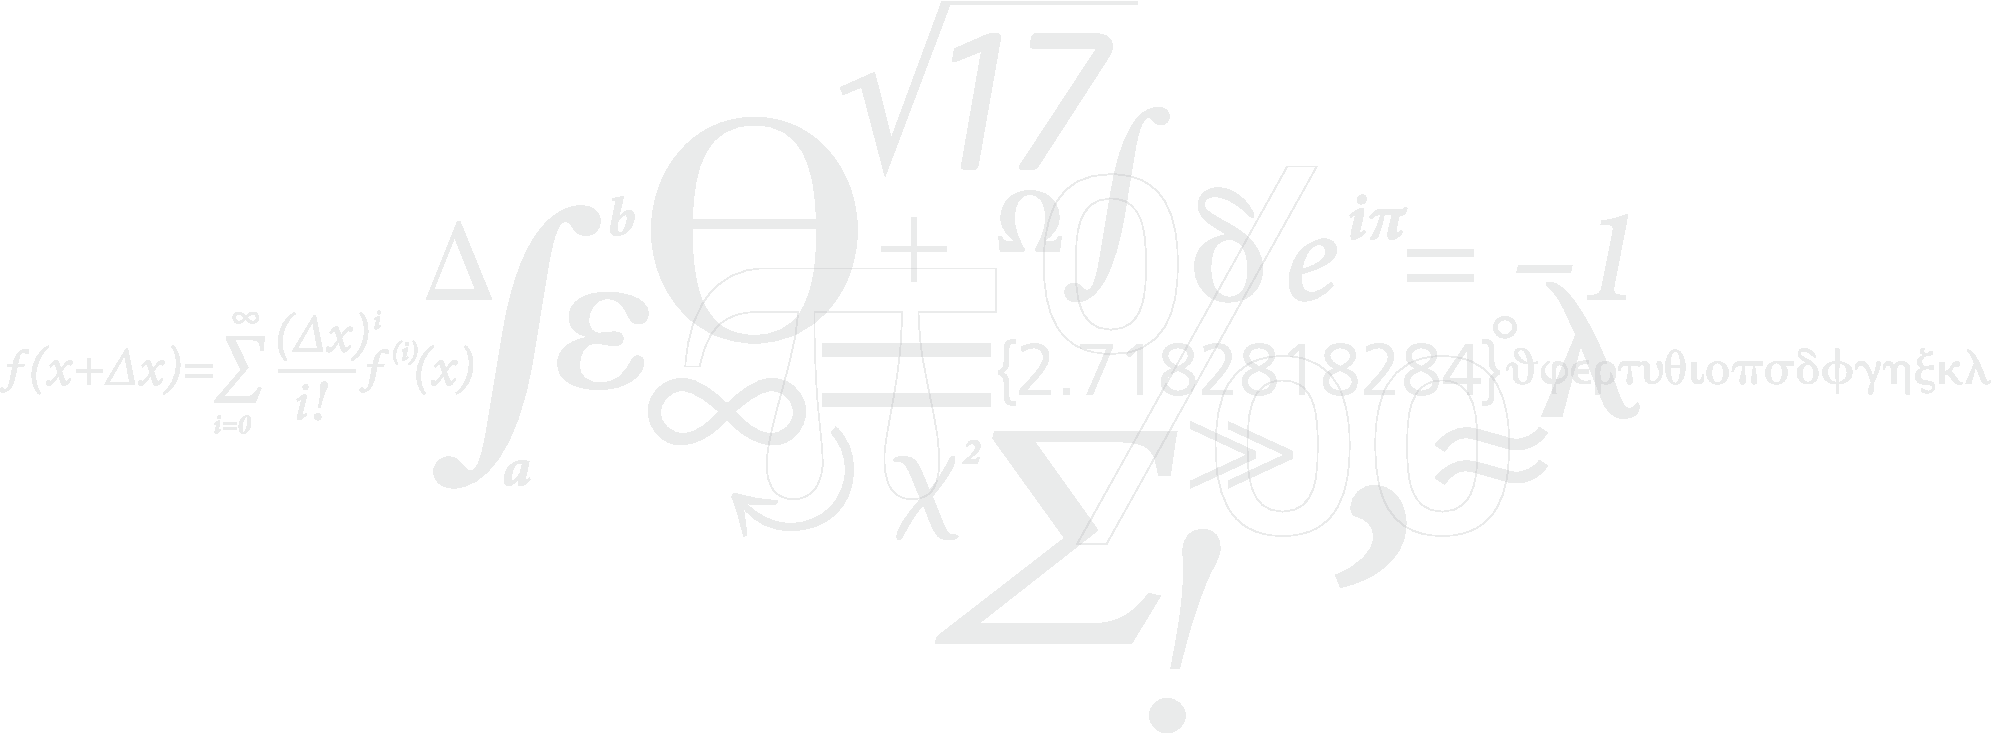
\includegraphics[trim=130mm 0 0 0,width=0.9\textwidth]{DTU-frise-SH-15}
                \vspace*{2.5cm}
            }
        }
    }
}

% This is a double sided book. If there is a last empty page lets use it for some fun e.g. the frieze.
% NB: For a fully functional hack the \clearpage used in \include does some odd things with the sequence numbering. Thefore use \input instead of \include at the end of the book. If bibliography is used at last everything should be ok.
\makeatletter
% Adjust so gatherings is allowd for single sheets too! (hacking functions in memoir.dtx)
\patchcmd{\leavespergathering}{\ifnum\@memcnta<\tw@}{\ifnum\@memcnta<\@ne}{
    \leavespergathering{1}
    % Insert the frieze
    \patchcmd{\@memensuresigpages}{\repeat}{\repeat\frieze{0}{0}}{}{}
}{}
\makeatother


% %% Sharelatex fix for microtype warnings
% \makeatletter
% \def\MT@is@composite#1#2\relax{%
%   \ifx\\#2\\\else
%     \expandafter\def\expandafter\MT@char\expandafter{\csname\expandafter
%                     \string\csname\MT@encoding\endcsname
%                     \MT@detokenize@n{#1}-\MT@detokenize@n{#2}\endcsname}%
%     % 3 lines added:
%     \ifx\UnicodeEncodingName\@undefined\else
%       \expandafter\expandafter\expandafter\MT@is@uni@comp\MT@char\iffontchar\else\fi\relax
%     \fi
%     \expandafter\expandafter\expandafter\MT@is@letter\MT@char\relax\relax
%     \ifnum\MT@char@ < \z@
%       \ifMT@xunicode
%         \edef\MT@char{\MT@exp@two@c\MT@strip@prefix\meaning\MT@char>\relax}%
%           \expandafter\MT@exp@two@c\expandafter\MT@is@charx\expandafter
%             \MT@char\MT@charxstring\relax\relax\relax\relax\relax
%       \fi
%     \fi
%   \fi
% }
% % new:
% \def\MT@is@uni@comp#1\iffontchar#2\else#3\fi\relax{%
%   \ifx\\#2\\\else\edef\MT@char{\iffontchar#2\fi}\fi
% }
% \makeatother\makeatother

%!TEX root = ../thesis.tex

% Text fonts (http://www.macfreek.nl/memory/Fonts_in_LaTeX)
% Install fonts from /usr/local/texlive/<version>/texmf-dist/fonts/opentype/public
\usepackage{fontspec}
\usepackage[T1]{fontenc}
\usepackage{lmodern}
\usepackage{slantsc}
% \RequirePackage{fix-cm}
\usepackage{bold-extra}
\usepackage{upgreek}

% \DeclareFontShape{T1}{texgyrepagella}{b}{sc}{<->ssub*cmr/bx/sc}{}
% \DeclareFontShape{T1}{texgyrepagella}{bx}{sc}{<->ssub*cmr/bx/sc}{}


% % Euler math fonts
% \usepackage[OT1,euler-digits,euler-hat-accent]{eulervm}
% \usepackage[bb=stixtwo]{mathalpha}
% \renewcommand{\mathbf}{\mathbold}  % euler requires \mathbold for bold math

% \usepackage{newtxmath}



% Serif font
% \usepackage{newpxtext}
% \setmainfont{TeX Gyre Pagella}
% \setmainfont{texgyrepagella}



\usepackage{mathpazo} % add possibly `sc` and `osf` options
\usepackage{eulervm}
\renewcommand{\mathbf}{\mathbold}  % euler requires \mathbold for bold math

% % Remove: "Font shape `T1/eulervm/m/n' undefined (Font) using `T1/cmr/m/n' instead."
% \usepackage{substitutefont}
% \substitutefont{TS1}{eulervm}{cmr}

%
% [
%   Extension=.otf,
%   UprightFont=*-regular,
%   ItalicFont=*-italic,
%   BoldFont=*-bold,
%   BoldItalicFont=*-bolditalic,
%   BoldSmallCapsFont=*-boldsmallcaps,
%   Numbers=OldStyle,
% ]

% \setmainfont{QTPalatine}

% \DeclareCharacterInheritance
%    { encoding = {TU,EU1,EU2},
%      family   = {QTPalatine} }
%    { A = {\`A,\'A,\^A,\~A,\"A,\r A},
%      a = {\`a,\'a,\^a,\~a,\"a,\r a},
%      C = {\c C},
%      c = {\c c},
%      D = {\DH},
%      d = {\dj},
%      E = {\`E,\'E,\^E,\"E},
%      e = {\`e,\'e,\^e,\"e},
%      I = {\`I,\'I,\^I,\"I},
%      i = {\`i,\'i,\^i,\"i,\i},
%      L = {\L},
%      l = {\l},
%      N = {\~N},
%      n = {\~n},
%      O = {\O,\`O,\'O,\^O,\~O,\"O},
%      o = {\o,\`o,\'o,\^o,\~o,\"o},
%      S = {\v S},
%      s = {\v s},
%      U = {\`U,\'U,\^U,\"U},
%      u = {\`u,\'u,\^u,\"u},
%      Y = {\'Y,\"Y},
%      y = {\'y,\"y},
%      Z = {\v Z},
%      z = {\v z}
%    }


% % Sans-serif font
% \setsansfont[
%     Ligatures=TeX,
%     Extension=.otf,
%     UprightFont=*-regular,
%     BoldFont=*-bold,
%     ItalicFont=*-italic,
%     BoldItalicFont=*-bolditalic,
%     % SlantedFont=,
%     % BoldSlantedFont=,
%     % SmallCapsFont=
%     Scale=0.8      % Adjustmens when using math in sections
% ]{texgyreadventor}


% Monospaced
% \setmonofont[Scale=MatchLowercase]{Linux Biolinum O}

%\setsansfont[Ligatures=TeX]{Neo Sans Intel}    % Neo Sans Intel – Like DTU font but more symbols
%\setsansfont[
%    Ligatures=TeX,
%    Scale=0.8
%]{NeoSans}           % NeoSans – DTU font (missing `+' symbols and other)
% \setsansfont[Ligatures=TeX]{CMU Sans Serif}    % Computer Modern Unicode font
%\setsansfont[Ligatures=TeX]{Latin Modern Sans} % Latin Modern Sans serif font

% Use this for more convienent sans serif font in math mode.
%\setmathsf{Latin Modern Sans}

%!TEX root = ../thesis.tex

% Content specific packages.

\usepackage{blindtext}
\usepackage{algorithm}
\usepackage{algpseudocode}
\usepackage{multicol}
\usepackage{multirow}
\usepackage{makecell}
\usepackage{booktabs}
\usepackage{enumerate}
\usepackage{enumitem}
% \usepackage{layouts}
\usepackage[showframe=\showframe,xetex]{geometry}
\usepackage{adjustbox}
\usepackage{siunitx}
\usepackage{nomencl}
\usepackage{amsmath}
\usepackage{amssymb}
\usepackage[acronym,toc]{glossaries}
%!TEX root = ../thesis.tex

% \makeglossaries
\makenoidxglossaries


% Glossary

\newglossaryentry{encoder}
{
    name=encoder,
    description={A general term for a function that maps an input to a different representation.}
}

\newglossaryentry{decoder}
{
    name=decoder,
    description={A general term for a function that maps a representation to an output.}
}


% Abbreviations
\newacronym{AI}{AI}{artificial intelligence}

\newacronym{MLP}{MLP}{multilayer perceptron}
\newacronym{FNN}{FNN}{feedforward neural network}
\newacronym{CNN}{CNN}{convolutional neural network}
\newacronym{RNN}{RNN}{recurrent neural network}
\newacronym{LSTM}{LSTM}{long short-term memory}
\newacronym{GRU}{GRU}{gated recurrent unit}
\newacronym{BNN}{BNN}{Bayesian neural network}

\newacronym{ReLU}{ReLU}{rectified linear unit}

\newacronym{SGD}{SGD}{stochastic gradient descent}

\newacronym{SGVB}{SGVB}{stochastic gradient variational Bayes}
\newacronym{VAE}{VAE}{variational autoencoder}
\newacronym{LVM}{LVM}{latent variable model}
\newacronym{KL}{KL}{Kullback-Leibler}

\newacronym{NLL}{NLL}{negative log-likelihood}
\newacronym{MSE}{MSE}{mean squared error}
\newacronym{CCE}{CCE}{categorical cross entropy}
\newacronym{MLE}{MLE}{maximum likelihood estimate}

\newacronym{PCA}{PCA}{principal components analysis}

\newacronym{PDF}{PDF}{probability density function}
\newacronym{PMF}{PMF}{probability mass function}

\newacronym{iid}{iid}{independent and identically distributed}

\newacronym{CPU}{CPU}{central processing unit}
\newacronym{GPU}{GPU}{graphics processing unit}
\newacronym{HPC}{HPC}{high performance computing}



%\usepackage{pgfplots}                 % Plot tools
%\pgfplotsset{compat=1.7}
\usetikzlibrary{
    arrows,
    matrix,
    positioning,
    shapes,
    shapes.multipart,
    topaths,
    bayesnet,
}
% tikzlibrary.code.tex
%
% Copyright 2010-2011 by Laura Dietz
% Copyright 2012 by Jaakko Luttinen
%
% This file may be distributed and/or modified
%
% 1. under the LaTeX Project Public License and/or
% 2. under the GNU General Public License.
%
% See the files LICENSE_LPPL and LICENSE_GPL for more details.

% Load other libraries
\usetikzlibrary{shapes}
\usetikzlibrary{fit}
\usetikzlibrary{chains}
\usetikzlibrary{arrows}

% Latent node
\tikzstyle{latent} = [circle,fill=white,draw=black,inner sep=1pt,
minimum size=20pt, font=\fontsize{10}{10}\selectfont, node distance=1]
% Observed node
\tikzstyle{obs} = [latent,fill=gray!25]
% Constant node
\tikzstyle{const} = [rectangle, inner sep=0pt, node distance=1]
% Factor node
\tikzstyle{factor} = [rectangle, fill=black,minimum size=5pt, inner
sep=0pt, node distance=0.4]
% Deterministic node
\tikzstyle{det} = [latent, diamond]

% Plate node
\tikzstyle{plate} = [draw, rectangle, rounded corners, fit=#1]
% Invisible wrapper node
\tikzstyle{wrap} = [inner sep=0pt, fit=#1]
% Gate
\tikzstyle{gate} = [draw, rectangle, dashed, fit=#1]

% Caption node
\tikzstyle{caption} = [font=\footnotesize, node distance=0] %
\tikzstyle{plate caption} = [caption, node distance=0, inner sep=0pt,
below left=5pt and 0pt of #1.south east] %
\tikzstyle{factor caption} = [caption] %
\tikzstyle{every label} += [caption] %

\tikzset{>={triangle 45}}

%\pgfdeclarelayer{b}
%\pgfdeclarelayer{f}
%\pgfsetlayers{b,main,f}

% \factoredge [options] {inputs} {factors} {outputs}
\renewcommand{\factoredge}[4][]{ %
  % Connect all nodes #2 to all nodes #4 via all factors #3.
  \foreach \f in {#3} { %
    \foreach \x in {#2} { %
      \path (\x) edge[-,#1] (\f) ; %
      %\draw[-,#1] (\x) edge[-] (\f) ; %
    } ;
    \foreach \y in {#4} { %
      \path (\f) edge[->,#1] (\y) ; %
      %\draw[->,#1] (\f) -- (\y) ; %
    } ;
  } ;
}

% \edge [options] {inputs} {outputs}
\renewcommand{\edge}[3][]{ %
  % Connect all nodes #2 to all nodes #3.
  \foreach \x in {#2} { %
    \foreach \y in {#3} { %
      \path (\x) edge [->,#1] (\y) ;%
      %\draw[->,#1] (\x) -- (\y) ;%
    } ;
  } ;
}

% \factor [options] {name} {caption} {inputs} {outputs}
\renewcommand{\factor}[5][]{ %
  % Draw the factor node. Use alias to allow empty names.
  \node[factor, label={[name=#2-caption]#3}, name=#2, #1,
  alias=#2-alias] {} ; %
  % Connect all inputs to outputs via this factor
  \factoredge {#4} {#2-alias} {#5} ; %
}

% \plate [options] {name} {fitlist} {caption}
\renewcommand{\plate}[4][]{ %
  \node[wrap=#3] (#2-wrap) {}; %
  \node[plate caption=#2-wrap] (#2-caption) {#4}; %
  \node[plate=(#2-wrap)(#2-caption), #1] (#2) {}; %
}

% \gate [options] {name} {fitlist} {inputs}
\renewcommand{\gate}[4][]{ %
  \node[gate=#3, name=#2, #1, alias=#2-alias] {}; %
  \foreach \x in {#4} { %
    \draw [-*,thick] (\x) -- (#2-alias); %
  } ;%
}

% \vgate {name} {fitlist-left} {caption-left} {fitlist-right}
% {caption-right} {inputs}
\renewcommand{\vgate}[6]{ %
  % Wrap the left and right parts
  \node[wrap=#2] (#1-left) {}; %
  \node[wrap=#4] (#1-right) {}; %
  % Draw the gate
  \node[gate=(#1-left)(#1-right)] (#1) {}; %
  % Add captions
  \node[caption, below left=of #1.north ] (#1-left-caption)
  {#3}; %
  \node[caption, below right=of #1.north ] (#1-right-caption)
  {#5}; %
  % Draw middle separation
  \draw [-, dashed] (#1.north) -- (#1.south); %
  % Draw inputs
  \foreach \x in {#6} { %
    \draw [-*,thick] (\x) -- (#1); %
  } ;%
}

% \hgate {name} {fitlist-top} {caption-top} {fitlist-bottom}
% {caption-bottom} {inputs}
\renewcommand{\hgate}[6]{ %
  % Wrap the left and right parts
  \node[wrap=#2] (#1-top) {}; %
  \node[wrap=#4] (#1-bottom) {}; %
  % Draw the gate
  \node[gate=(#1-top)(#1-bottom)] (#1) {}; %
  % Add captions
  \node[caption, above right=of #1.west ] (#1-top-caption)
  {#3}; %
  \node[caption, below right=of #1.west ] (#1-bottom-caption)
  {#5}; %
  % Draw middle separation
  \draw [-, dashed] (#1.west) -- (#1.east); %
  % Draw inputs
  \foreach \x in {#6} { %
    \draw [-*,thick] (\x) -- (#1); %
  } ;%
}



\definecolor{customgreen} {RGB}{217	234	212}
\definecolor{customblue}  {RGB}{205	226	242}
\definecolor{custommorered}{RGB}{218 46 42}
\definecolor{customred}{RGB}{255 182 173}%{255 149 150}

\colorlet{observed-color}{customgreen}
\colorlet{latent-color}{customblue}
\colorlet{deterministic-color}{gray!15}
\colorlet{deterministic-skip-color}{custommorered}
\colorlet{shared-function-color}{blue}


% Listings
\lstset{
    basicstyle=\footnotesize\ttfamily,% the size of the fonts that are used for the code
    breakatwhitespace=false,          % sets if automatic breaks should only happen at whitespace
    breaklines=true,                  % sets automatic line breaking
    captionpos=b,                     % sets the caption-position to bottom
    commentstyle=\color{s14a},        % comment style
    deletekeywords={},                % if you want to delete keywords from the given language
    escapeinside={\%*}{*)},           % if you want to add LaTeX within your code
    frame=single,                     % adds a frame around the code
    keywordstyle=\bfseries\ttfamily\color{s09}, % keyword style
    language=Python,                  % the language of the code
    morekeywords={*,...},             % if you want to add more keywords to the set
    numbers=left,                     % where to put the line-numbers; possible values are (none, left, right)
    numbersep=5pt,                    % how far the line-numbers are from the code
    numberstyle=\sffamily\tiny\color{dtugray}, % the style that is used for the line-numbers
    rulecolor=\color{dtugray},        % if not set, the frame-color may be changed on line-breaks within not-black text (e.g. comments (green here))
    showspaces=false,                 % show spaces everywhere adding particular underscores; it overrides 'showstringspaces'
    showstringspaces=false,           % underline spaces within strings only
    showtabs=false,                   % show tabs within strings adding particular underscores
    stepnumber=1,                     % the step between two line-numbers. If it's 1, each line will be numbered
    stringstyle=\color{s07},          % string literal style
    tabsize=2,                        % sets default tabsize to 2 spaces
    title=\lstname,                   % show the filename of files included with \lstinputlisting; also try caption instead of title
}


%!TEX root = ../thesis.tex

% \makeglossaries
\makenoidxglossaries


% Glossary

\newglossaryentry{encoder}
{
    name=encoder,
    description={A general term for a function that maps an input to a different representation.}
}

\newglossaryentry{decoder}
{
    name=decoder,
    description={A general term for a function that maps a representation to an output.}
}


% Abbreviations
\newacronym{AI}{AI}{artificial intelligence}

\newacronym{MLP}{MLP}{multilayer perceptron}
\newacronym{FNN}{FNN}{feedforward neural network}
\newacronym{CNN}{CNN}{convolutional neural network}
\newacronym{RNN}{RNN}{recurrent neural network}
\newacronym{LSTM}{LSTM}{long short-term memory}
\newacronym{GRU}{GRU}{gated recurrent unit}
\newacronym{BNN}{BNN}{Bayesian neural network}

\newacronym{ReLU}{ReLU}{rectified linear unit}

\newacronym{SGD}{SGD}{stochastic gradient descent}

\newacronym{SGVB}{SGVB}{stochastic gradient variational Bayes}
\newacronym{VAE}{VAE}{variational autoencoder}
\newacronym{LVM}{LVM}{latent variable model}
\newacronym{KL}{KL}{Kullback-Leibler}

\newacronym{NLL}{NLL}{negative log-likelihood}
\newacronym{MSE}{MSE}{mean squared error}
\newacronym{CCE}{CCE}{categorical cross entropy}
\newacronym{MLE}{MLE}{maximum likelihood estimate}

\newacronym{PCA}{PCA}{principal components analysis}

\newacronym{PDF}{PDF}{probability density function}
\newacronym{PMF}{PMF}{probability mass function}

\newacronym{iid}{iid}{independent and identically distributed}

\newacronym{CPU}{CPU}{central processing unit}
\newacronym{GPU}{GPU}{graphics processing unit}
\newacronym{HPC}{HPC}{high performance computing}

%!TEX root = ../thesis.tex

% Parenthesis
\providecommand{\pa}[1]{{\left(#1\right)}}
  \renewcommand{\pa}[1]{{\left(#1\right)}}
\providecommand{\bra}[1]{{\left[#1\right]}}
  \renewcommand{\bra}[1]{{\left[#1\right]}}
\providecommand{\cbra}[1]{{\left\{#1\right\}}}
  \renewcommand{\cbra}[1]{{\left\{#1\right\}}}
\providecommand{\vbra}[1]{{\left\langle#1\right\rangle}}
  \renewcommand{\vbra}[1]{{\left\langle#1\right\rangle}}

% Matrices for displayed expressions
\providecommand{\mat}[1]{{\begin{matrix}#1\end{matrix}}}
  \renewcommand{\mat}[1]{{\begin{matrix}#1\end{matrix}}}
\providecommand{\pmat}[1]{{\begin{pmatrix}#1\end{pmatrix}}}
  \renewcommand{\pmat}[1]{{\begin{pmatrix}#1\end{pmatrix}}}
\providecommand{\bmat}[1]{{\begin{bmatrix}#1\end{bmatrix}}}
  \renewcommand{\bmat}[1]{{\begin{bmatrix}#1\end{bmatrix}}}

% Variations of \frac and \sfrac
\providecommand{\pfrac}[2]{{\left(\frac{#1}{#2}\right)}}
  \renewcommand{\pfrac}[2]{{\left(\frac{#1}{#2}\right)}}
\providecommand{\bfrac}[2]{{\left[\frac{#1}{#2}\right]}}
  \renewcommand{\bfrac}[2]{{\left[\frac{#1}{#2}\right]}}
\providecommand{\psfrac}[2]{{\left(\sfrac{#1}{#2}\right)}}
  \renewcommand{\psfrac}[2]{{\left(\sfrac{#1}{#2}\right)}}
\providecommand{\bsfrac}[2]{{\left[\sfrac{#1}{#2}\right]}}
  \renewcommand{\bsfrac}[2]{{\left[\sfrac{#1}{#2}\right]}}

% for small matrices to be used in in-line expressions
\providecommand{\sm}[1]{{\left\{#1\right\}}}
  \renewcommand{\sm}[1]{{\left\{#1\right\}}}
\providecommand{\psm}[1]{{\pa{\sm{#1}}}}
  \renewcommand{\psm}[1]{{\pa{\sm{#1}}}}
\providecommand{\bsm}[1]{{\bra{\sm{#1}}}}
  \renewcommand{\bsm}[1]{{\bra{\sm{#1}}}}

% Norm
\providecommand{\norm}[1]{{\left\lVert#1\right\rVert}}
  \renewcommand{\norm}[1]{{\left\lVert#1\right\rVert}}
% Size
\providecommand{\size}[1]{{\left\lvert#1\right\rvert}}
  \renewcommand{\size}[1]{{\left\lvert#1\right\rvert}}
% Trace
\providecommand{\Tr}[1]{{\text{Tr}\left[#1\right]}}
  \renewcommand{\Tr}[1]{{\text{Tr}\left[#1\right]}}
% Tranpose
\providecommand{\transpose}{{^\mathrm{T}}}
  \renewcommand{\transpose}{{^\mathrm{T}}}

% Derivatives
\providecommand{\od}[3][]{{\frac{\text{d}^{#1}#2}{\text{d}^{#1}#3}}}
  \renewcommand{\od}[3][]{{\frac{\text{d}^{#1}#2}{\text{d}^{#1}#3}}}
\providecommand{\pd}[3][]{{\frac{\partial^{#1}#2}{\partial^{#1}#3}}}
  \renewcommand{\pd}[3][]{{\frac{\partial^{#1}#2}{\partial^{#1}#3}}}

% Bold upright letters
\providecommand{\ab}{{\mathbf{a}}}
  \renewcommand{\ab}{{\mathbf{a}}}
\providecommand{\bb}{{\mathbf{b}}}
  \renewcommand{\bb}{{\mathbf{b}}}
\providecommand{\cb}{{\mathbf{c}}}
  \renewcommand{\cb}{{\mathbf{c}}}
\providecommand{\db}{{\mathbf{d}}}
  \renewcommand{\db}{{\mathbf{d}}}
\providecommand{\eb}{{\mathbf{e}}}
  \renewcommand{\eb}{{\mathbf{e}}}
\providecommand{\fb}{{\mathbf{f}}}
  \renewcommand{\fb}{{\mathbf{f}}}
\providecommand{\gb}{{\mathbf{g}}}
  \renewcommand{\gb}{{\mathbf{g}}}
\providecommand{\hb}{{\mathbf{h}}}
  \renewcommand{\hb}{{\mathbf{h}}}
\providecommand{\ib}{{\mathbf{i}}}
  \renewcommand{\ib}{{\mathbf{i}}}
\providecommand{\jb}{{\mathbf{j}}}
  \renewcommand{\jb}{{\mathbf{j}}}
\providecommand{\kb}{{\mathbf{k}}}
  \renewcommand{\kb}{{\mathbf{k}}}
\providecommand{\lb}{{\mathbf{l}}}
  \renewcommand{\lb}{{\mathbf{l}}}
\providecommand{\mb}{{\mathbf{m}}}
  \renewcommand{\mb}{{\mathbf{m}}}
\providecommand{\nb}{{\mathbf{n}}}
  \renewcommand{\nb}{{\mathbf{n}}}
\providecommand{\ob}{{\mathbf{o}}}
  \renewcommand{\ob}{{\mathbf{o}}}
\providecommand{\pb}{{\mathbf{p}}}
  \renewcommand{\pb}{{\mathbf{p}}}
\providecommand{\qb}{{\mathbf{q}}}
  \renewcommand{\qb}{{\mathbf{q}}}
\providecommand{\rb}{{\mathbf{r}}}
  \renewcommand{\rb}{{\mathbf{r}}}
\providecommand{\vs}{{\mathbf{s}}}
  \renewcommand{\vs}{{\mathbf{s}}}
\providecommand{\tb}{{\mathbf{t}}}
  \renewcommand{\tb}{{\mathbf{t}}}
\providecommand{\ub}{{\mathbf{u}}}
  \renewcommand{\ub}{{\mathbf{u}}}
\providecommand{\vb}{{\mathbf{v}}}
  \renewcommand{\vb}{{\mathbf{v}}}
\providecommand{\wb}{{\mathbf{w}}}
  \renewcommand{\wb}{{\mathbf{w}}}
\providecommand{\xb}{{\mathbf{x}}}
  \renewcommand{\xb}{{\mathbf{x}}}
\providecommand{\yb}{{\mathbf{y}}}
  \renewcommand{\yb}{{\mathbf{y}}}
\providecommand{\zb}{{\mathbf{z}}}
  \renewcommand{\zb}{{\mathbf{z}}}
\providecommand{\Ab}{{\mathbf{A}}}
  \renewcommand{\Ab}{{\mathbf{A}}}
\providecommand{\Bb}{{\mathbf{B}}}
  \renewcommand{\Bb}{{\mathbf{B}}}
\providecommand{\Cb}{{\mathbf{C}}}
  \renewcommand{\Cb}{{\mathbf{C}}}
\providecommand{\Db}{{\mathbf{D}}}
  \renewcommand{\Db}{{\mathbf{D}}}
\providecommand{\Eb}{{\mathbf{E}}}
  \renewcommand{\Eb}{{\mathbf{E}}}
\providecommand{\Fb}{{\mathbf{F}}}
  \renewcommand{\Fb}{{\mathbf{F}}}
\providecommand{\Gb}{{\mathbf{G}}}
  \renewcommand{\Gb}{{\mathbf{G}}}
\providecommand{\Hb}{{\mathbf{H}}}
  \renewcommand{\Hb}{{\mathbf{H}}}
\providecommand{\Ib}{{\mathbf{I}}}
  \renewcommand{\Ib}{{\mathbf{I}}}
\providecommand{\Jb}{{\mathbf{J}}}
  \renewcommand{\Jb}{{\mathbf{J}}}
\providecommand{\Kb}{{\mathbf{K}}}
  \renewcommand{\Kb}{{\mathbf{K}}}
\providecommand{\Lb}{{\mathbf{L}}}
  \renewcommand{\Lb}{{\mathbf{L}}}
\providecommand{\Mb}{{\mathbf{M}}}
  \renewcommand{\Mb}{{\mathbf{M}}}
\providecommand{\Nb}{{\mathbf{N}}}
  \renewcommand{\Nb}{{\mathbf{N}}}
\providecommand{\Ob}{{\mathbf{O}}}
  \renewcommand{\Ob}{{\mathbf{O}}}
\providecommand{\Pb}{{\mathbf{P}}}
  \renewcommand{\Pb}{{\mathbf{P}}}
\providecommand{\Qb}{{\mathbf{Q}}}
  \renewcommand{\Qb}{{\mathbf{Q}}}
\providecommand{\Rb}{{\mathbf{R}}}
  \renewcommand{\Rb}{{\mathbf{R}}}
\providecommand{\Sb}{{\mathbf{S}}}
  \renewcommand{\Sb}{{\mathbf{S}}}
\providecommand{\Tb}{{\mathbf{T}}}
  \renewcommand{\Tb}{{\mathbf{T}}}
\providecommand{\Ub}{{\mathbf{U}}}
  \renewcommand{\Ub}{{\mathbf{U}}}
\providecommand{\Vb}{{\mathbf{V}}}
  \renewcommand{\Vb}{{\mathbf{V}}}
\providecommand{\Wb}{{\mathbf{W}}}
  \renewcommand{\Wb}{{\mathbf{W}}}
\providecommand{\Xb}{{\mathbf{X}}}
  \renewcommand{\Xb}{{\mathbf{X}}}
\providecommand{\Yb}{{\mathbf{Y}}}
  \renewcommand{\Yb}{{\mathbf{Y}}}
\providecommand{\Zb}{{\mathbf{Z}}}
  \renewcommand{\Zb}{{\mathbf{Z}}}
% Bold upright numbers
\providecommand{\0}{{\mathbf{0}}}
  \renewcommand{\0}{{\mathbf{0}}}
\providecommand{\1}{{\mathbf{1}}}
  \renewcommand{\1}{{\mathbf{1}}}
\providecommand{\2}{{\mathbf{2}}}
  \renewcommand{\2}{{\mathbf{2}}}
\providecommand{\3}{{\mathbf{3}}}
  \renewcommand{\3}{{\mathbf{3}}}
\providecommand{\4}{{\mathbf{4}}}
  \renewcommand{\4}{{\mathbf{4}}}
\providecommand{\5}{{\mathbf{5}}}
  \renewcommand{\5}{{\mathbf{5}}}
\providecommand{\6}{{\mathbf{6}}}
  \renewcommand{\6}{{\mathbf{6}}}
\providecommand{\7}{{\mathbf{7}}}
  \renewcommand{\7}{{\mathbf{7}}}
\providecommand{\8}{{\mathbf{8}}}
  \renewcommand{\8}{{\mathbf{8}}}
\providecommand{\9}{{\mathbf{9}}}
  \renewcommand{\9}{{\mathbf{9}}}
% Bold upright greek symbols
\providecommand{\alphab}{{\boldsymbol{\upalpha}}}
  \renewcommand{\alphab}{{\boldsymbol{\upalpha}}}
\providecommand{\thetab}{{\boldsymbol{\uptheta}}}
  \renewcommand{\thetab}{{\boldsymbol{\uptheta}}}
\providecommand{\taub}{{\boldsymbol{\uptau}}}
  \renewcommand{\taub}{{\boldsymbol{\uptau}}}
\providecommand{\betab}{{\boldsymbol{\upbeta}}}
  \renewcommand{\betab}{{\boldsymbol{\upbeta}}}
\providecommand{\varthetab}{{\boldsymbol{\upvartheta}}}
  \renewcommand{\varthetab}{{\boldsymbol{\upvartheta}}}
\providecommand{\pib}{{\boldsymbol{\uppi}}}
  \renewcommand{\pib}{{\boldsymbol{\uppi}}}
\providecommand{\upsilonb}{{\boldsymbol{\upupsilon}}}
  \renewcommand{\upsilonb}{{\boldsymbol{\upupsilon}}}
\providecommand{\gammab}{{\boldsymbol{\upgamma}}}
  \renewcommand{\gammab}{{\boldsymbol{\upgamma}}}
\providecommand{\gammab}{{\boldsymbol{\upgamma}}}
  \renewcommand{\gammab}{{\boldsymbol{\upgamma}}}
\providecommand{\varpib}{{\boldsymbol{\upvarpi}}}
  \renewcommand{\varpib}{{\boldsymbol{\upvarpi}}}
\providecommand{\phib}{{\boldsymbol{\upphi}}}
  \renewcommand{\phib}{{\boldsymbol{\upphi}}}
\providecommand{\deltab}{{\boldsymbol{\updelta}}}
  \renewcommand{\deltab}{{\boldsymbol{\updelta}}}
\providecommand{\kappab}{{\boldsymbol{\upkappa}}}
  \renewcommand{\kappab}{{\boldsymbol{\upkappa}}}
\providecommand{\rhob}{{\boldsymbol{\uprho}}}
  \renewcommand{\rhob}{{\boldsymbol{\uprho}}}
\providecommand{\varphib}{{\boldsymbol{\upvarphi}}}
  \renewcommand{\varphib}{{\boldsymbol{\upvarphi}}}
\providecommand{\epsilonb}{{\boldsymbol{\upepsilon}}}
  \renewcommand{\epsilonb}{{\boldsymbol{\upepsilon}}}
\providecommand{\lambdab}{{\boldsymbol{\uplambda}}}
  \renewcommand{\lambdab}{{\boldsymbol{\uplambda}}}
\providecommand{\varrhob}{{\boldsymbol{\upvarrho}}}
  \renewcommand{\varrhob}{{\boldsymbol{\upvarrho}}}
\providecommand{\chib}{{\boldsymbol{\upchi}}}
  \renewcommand{\chib}{{\boldsymbol{\upchi}}}
\providecommand{\varepsilonb}{{\boldsymbol{\upvarepsilon}}}
  \renewcommand{\varepsilonb}{{\boldsymbol{\upvarepsilon}}}
\providecommand{\mub}{{\boldsymbol{\upmu}}}
  \renewcommand{\mub}{{\boldsymbol{\upmu}}}
\providecommand{\sigmab}{{\boldsymbol{\upsigma}}}
  \renewcommand{\sigmab}{{\boldsymbol{\upsigma}}}
\providecommand{\psib}{{\boldsymbol{\uppsi}}}
  \renewcommand{\psib}{{\boldsymbol{\uppsi}}}
\providecommand{\zetab}{{\boldsymbol{\upzeta}}}
  \renewcommand{\zetab}{{\boldsymbol{\upzeta}}}
\providecommand{\nub}{{\boldsymbol{\upnu}}}
  \renewcommand{\nub}{{\boldsymbol{\upnu}}}
\providecommand{\varsigmab}{{\boldsymbol{\upvarsigma}}}
  \renewcommand{\varsigmab}{{\boldsymbol{\upvarsigma}}}
\providecommand{\omegab}{{\boldsymbol{\upomega}}}
  \renewcommand{\omegab}{{\boldsymbol{\upomega}}}
\providecommand{\etab}{{\boldsymbol{\upeta}}}
  \renewcommand{\etab}{{\boldsymbol{\upeta}}}
\providecommand{\xib}{{\boldsymbol{\upxi}}}
  \renewcommand{\xib}{{\boldsymbol{\upxi}}}
\providecommand{\Gammab}{{\boldsymbol{\Upgamma}}}
  \renewcommand{\Gammab}{{\boldsymbol{\Upgamma}}}
\providecommand{\Lambdab}{{\boldsymbol{\Uplambda}}}
  \renewcommand{\Lambdab}{{\boldsymbol{\Uplambda}}}
\providecommand{\Sigmab}{{\boldsymbol{\Upsigma}}}
  \renewcommand{\Sigmab}{{\boldsymbol{\Upsigma}}}
\providecommand{\Psib}{{\boldsymbol{\Uppsi}}}
  \renewcommand{\Psib}{{\boldsymbol{\Uppsi}}}
\providecommand{\Deltab}{{\boldsymbol{\Updelta}}}
  \renewcommand{\Deltab}{{\boldsymbol{\Updelta}}}
\providecommand{\Xib}{{\boldsymbol{\Upxi}}}
  \renewcommand{\Xib}{{\boldsymbol{\Upxi}}}
\providecommand{\Upsilonb}{{\boldsymbol{\Upupsilon}}}
  \renewcommand{\Upsilonb}{{\boldsymbol{\Upupsilon}}}
\providecommand{\Omegab}{{\boldsymbol{\Upomega}}}
  \renewcommand{\Omegab}{{\boldsymbol{\Upomega}}}
\providecommand{\Thetab}{{\boldsymbol{\Uptheta}}}
  \renewcommand{\Thetab}{{\boldsymbol{\Uptheta}}}
\providecommand{\Pib}{{\boldsymbol{\Uppi}}}
  \renewcommand{\Pib}{{\boldsymbol{\Uppi}}}
\providecommand{\Phib}{{\boldsymbol{\Upphi}}}
  \renewcommand{\Phib}{{\boldsymbol{\Upphi}}}

% Bold letters
\providecommand{\abs}{{{\boldsymbol{a}}}}
  \renewcommand{\abs}{{{\boldsymbol{a}}}}
\providecommand{\bbs}{{{\boldsymbol{b}}}}
  \renewcommand{\bbs}{{{\boldsymbol{b}}}}
\providecommand{\cbs}{{{\boldsymbol{c}}}}
  \renewcommand{\cbs}{{{\boldsymbol{c}}}}
\providecommand{\dbs}{{{\boldsymbol{d}}}}
  \renewcommand{\dbs}{{{\boldsymbol{d}}}}
\providecommand{\ebs}{{{\boldsymbol{e}}}}
  \renewcommand{\ebs}{{{\boldsymbol{e}}}}
\providecommand{\fbs}{{{\boldsymbol{f}}}}
  \renewcommand{\fbs}{{{\boldsymbol{f}}}}
\providecommand{\gbs}{{{\boldsymbol{g}}}}
  \renewcommand{\gbs}{{{\boldsymbol{g}}}}
\providecommand{\hbs}{{{\boldsymbol{h}}}}
  \renewcommand{\hbs}{{{\boldsymbol{h}}}}
\providecommand{\ibs}{{{\boldsymbol{i}}}}
  \renewcommand{\ibs}{{{\boldsymbol{i}}}}
\providecommand{\jbs}{{{\boldsymbol{j}}}}
  \renewcommand{\jbs}{{{\boldsymbol{j}}}}
\providecommand{\kbs}{{{\boldsymbol{k}}}}
  \renewcommand{\kbs}{{{\boldsymbol{k}}}}
\providecommand{\lbs}{{{\boldsymbol{l}}}}
  \renewcommand{\lbs}{{{\boldsymbol{l}}}}
\providecommand{\mbs}{{{\boldsymbol{m}}}}
  \renewcommand{\mbs}{{{\boldsymbol{m}}}}
\providecommand{\nbs}{{{\boldsymbol{n}}}}
  \renewcommand{\nbs}{{{\boldsymbol{n}}}}
\providecommand{\obs}{{{\boldsymbol{o}}}}
  \renewcommand{\obs}{{{\boldsymbol{o}}}}
\providecommand{\pbs}{{{\boldsymbol{p}}}}
  \renewcommand{\pbs}{{{\boldsymbol{p}}}}
\providecommand{\qbs}{{{\boldsymbol{q}}}}
  \renewcommand{\qbs}{{{\boldsymbol{q}}}}
\providecommand{\rbs}{{{\boldsymbol{r}}}}
  \renewcommand{\rbs}{{{\boldsymbol{r}}}}
\providecommand{\sbs}{{{\boldsymbol{s}}}}
  \renewcommand{\sbs}{{{\boldsymbol{s}}}}
\providecommand{\tbs}{{{\boldsymbol{t}}}}
  \renewcommand{\tbs}{{{\boldsymbol{t}}}}
\providecommand{\ubs}{{{\boldsymbol{u}}}}
  \renewcommand{\ubs}{{{\boldsymbol{u}}}}
\providecommand{\vbs}{{{\boldsymbol{v}}}}
  \renewcommand{\vbs}{{{\boldsymbol{v}}}}
\providecommand{\wbs}{{{\boldsymbol{w}}}}
  \renewcommand{\wbs}{{{\boldsymbol{w}}}}
\providecommand{\xbs}{{{\boldsymbol{x}}}}
  \renewcommand{\xbs}{{{\boldsymbol{x}}}}
\providecommand{\ybs}{{{\boldsymbol{y}}}}
  \renewcommand{\ybs}{{{\boldsymbol{y}}}}
\providecommand{\zbs}{{{\boldsymbol{z}}}}
  \renewcommand{\zbs}{{{\boldsymbol{z}}}}
\providecommand{\Abs}{{{\boldsymbol{A}}}}
  \renewcommand{\Abs}{{{\boldsymbol{A}}}}
\providecommand{\Bbs}{{{\boldsymbol{B}}}}
  \renewcommand{\Bbs}{{{\boldsymbol{B}}}}
\providecommand{\Cbs}{{{\boldsymbol{C}}}}
  \renewcommand{\Cbs}{{{\boldsymbol{C}}}}
\providecommand{\Dbs}{{{\boldsymbol{D}}}}
  \renewcommand{\Dbs}{{{\boldsymbol{D}}}}
\providecommand{\Ebs}{{{\boldsymbol{E}}}}
  \renewcommand{\Ebs}{{{\boldsymbol{E}}}}
\providecommand{\Fbs}{{{\boldsymbol{F}}}}
  \renewcommand{\Fbs}{{{\boldsymbol{F}}}}
\providecommand{\Gbs}{{{\boldsymbol{G}}}}
  \renewcommand{\Gbs}{{{\boldsymbol{G}}}}
\providecommand{\Hbs}{{{\boldsymbol{H}}}}
  \renewcommand{\Hbs}{{{\boldsymbol{H}}}}
\providecommand{\Ibs}{{{\boldsymbol{I}}}}
  \renewcommand{\Ibs}{{{\boldsymbol{I}}}}
\providecommand{\Jbs}{{{\boldsymbol{J}}}}
  \renewcommand{\Jbs}{{{\boldsymbol{J}}}}
\providecommand{\Kbs}{{{\boldsymbol{K}}}}
  \renewcommand{\Kbs}{{{\boldsymbol{K}}}}
\providecommand{\Lbs}{{{\boldsymbol{L}}}}
  \renewcommand{\Lbs}{{{\boldsymbol{L}}}}
\providecommand{\Mbs}{{{\boldsymbol{M}}}}
  \renewcommand{\Mbs}{{{\boldsymbol{M}}}}
\providecommand{\Nbs}{{{\boldsymbol{N}}}}
  \renewcommand{\Nbs}{{{\boldsymbol{N}}}}
\providecommand{\Obs}{{{\boldsymbol{O}}}}
  \renewcommand{\Obs}{{{\boldsymbol{O}}}}
\providecommand{\Pbs}{{{\boldsymbol{P}}}}
  \renewcommand{\Pbs}{{{\boldsymbol{P}}}}
\providecommand{\Qbs}{{{\boldsymbol{Q}}}}
  \renewcommand{\Qbs}{{{\boldsymbol{Q}}}}
\providecommand{\Rbs}{{{\boldsymbol{R}}}}
  \renewcommand{\Rbs}{{{\boldsymbol{R}}}}
\providecommand{\Sbs}{{{\boldsymbol{S}}}}
  \renewcommand{\Sbs}{{{\boldsymbol{S}}}}
\providecommand{\Tbs}{{{\boldsymbol{T}}}}
  \renewcommand{\Tbs}{{{\boldsymbol{T}}}}
\providecommand{\Ubs}{{{\boldsymbol{U}}}}
  \renewcommand{\Ubs}{{{\boldsymbol{U}}}}
\providecommand{\Vbs}{{{\boldsymbol{V}}}}
  \renewcommand{\Vbs}{{{\boldsymbol{V}}}}
\providecommand{\Wbs}{{{\boldsymbol{W}}}}
  \renewcommand{\Wbs}{{{\boldsymbol{W}}}}
\providecommand{\Xbs}{{{\boldsymbol{X}}}}
  \renewcommand{\Xbs}{{{\boldsymbol{X}}}}
\providecommand{\Ybs}{{{\boldsymbol{Y}}}}
  \renewcommand{\Ybs}{{{\boldsymbol{Y}}}}
\providecommand{\Zbs}{{{\boldsymbol{Z}}}}
  \renewcommand{\Zbs}{{{\boldsymbol{Z}}}}
% Bold greek symbols
\providecommand{\alphabs}{{{\boldsymbol{\alpha}}}}
  \renewcommand{\alphabs}{{{\boldsymbol{\alpha}}}}
\providecommand{\thetabs}{{{\boldsymbol{\theta}}}}
  \renewcommand{\thetabs}{{{\boldsymbol{\theta}}}}
\providecommand{\taubs}{{{\boldsymbol{\tau}}}}
  \renewcommand{\taubs}{{{\boldsymbol{\tau}}}}
\providecommand{\betabs}{{{\boldsymbol{\beta}}}}
  \renewcommand{\betabs}{{{\boldsymbol{\beta}}}}
\providecommand{\varthetabs}{{{\boldsymbol{\vartheta}}}}
  \renewcommand{\varthetabs}{{{\boldsymbol{\vartheta}}}}
\providecommand{\pibs}{{{\boldsymbol{\pi}}}}
  \renewcommand{\pibs}{{{\boldsymbol{\pi}}}}
\providecommand{\upsilonbs}{{{\boldsymbol{\upsilon}}}}
  \renewcommand{\upsilonbs}{{{\boldsymbol{\upsilon}}}}
\providecommand{\gammabs}{{{\boldsymbol{\gamma}}}}
  \renewcommand{\gammabs}{{{\boldsymbol{\gamma}}}}
\providecommand{\gammabs}{{{\boldsymbol{\gamma}}}}
  \renewcommand{\gammabs}{{{\boldsymbol{\gamma}}}}
\providecommand{\varpibs}{{{\boldsymbol{\varpi}}}}
  \renewcommand{\varpibs}{{{\boldsymbol{\varpi}}}}
\providecommand{\phibs}{{{\boldsymbol{\phi}}}}
  \renewcommand{\phibs}{{{\boldsymbol{\phi}}}}
\providecommand{\deltabs}{{{\boldsymbol{\delta}}}}
  \renewcommand{\deltabs}{{{\boldsymbol{\delta}}}}
\providecommand{\kappabs}{{{\boldsymbol{\kappa}}}}
  \renewcommand{\kappabs}{{{\boldsymbol{\kappa}}}}
\providecommand{\rhobs}{{{\boldsymbol{\rho}}}}
  \renewcommand{\rhobs}{{{\boldsymbol{\rho}}}}
\providecommand{\varphibs}{{{\boldsymbol{\varphi}}}}
  \renewcommand{\varphibs}{{{\boldsymbol{\varphi}}}}
\providecommand{\epsilonbs}{{{\boldsymbol{\epsilon}}}}
  \renewcommand{\epsilonbs}{{{\boldsymbol{\epsilon}}}}
\providecommand{\lambdabs}{{{\boldsymbol{\lambda}}}}
  \renewcommand{\lambdabs}{{{\boldsymbol{\lambda}}}}
\providecommand{\varrhobs}{{{\boldsymbol{\varrho}}}}
  \renewcommand{\varrhobs}{{{\boldsymbol{\varrho}}}}
\providecommand{\chibs}{{{\boldsymbol{\chi}}}}
  \renewcommand{\chibs}{{{\boldsymbol{\chi}}}}
\providecommand{\varepsilonbs}{{{\boldsymbol{\varepsilon}}}}
  \renewcommand{\varepsilonbs}{{{\boldsymbol{\varepsilon}}}}
\providecommand{\mubs}{{{\boldsymbol{\mu}}}}
  \renewcommand{\mubs}{{{\boldsymbol{\mu}}}}
\providecommand{\sigmabs}{{{\boldsymbol{\sigma}}}}
  \renewcommand{\sigmabs}{{{\boldsymbol{\sigma}}}}
\providecommand{\psibs}{{{\boldsymbol{\psi}}}}
  \renewcommand{\psibs}{{{\boldsymbol{\psi}}}}
\providecommand{\zetabs}{{{\boldsymbol{\zeta}}}}
  \renewcommand{\zetabs}{{{\boldsymbol{\zeta}}}}
\providecommand{\nubs}{{{\boldsymbol{\nu}}}}
  \renewcommand{\nubs}{{{\boldsymbol{\nu}}}}
\providecommand{\varsigmabs}{{{\boldsymbol{\varsigma}}}}
  \renewcommand{\varsigmabs}{{{\boldsymbol{\varsigma}}}}
\providecommand{\omegabs}{{{\boldsymbol{\omega}}}}
  \renewcommand{\omegabs}{{{\boldsymbol{\omega}}}}
\providecommand{\etabs}{{{\boldsymbol{\eta}}}}
  \renewcommand{\etabs}{{{\boldsymbol{\eta}}}}
\providecommand{\xibs}{{{\boldsymbol{\xi}}}}
  \renewcommand{\xibs}{{{\boldsymbol{\xi}}}}
\providecommand{\Gammabs}{{{\boldsymbol{\Gamma}}}}
  \renewcommand{\Gammabs}{{{\boldsymbol{\Gamma}}}}
\providecommand{\Lambdabs}{{{\boldsymbol{\Lambda}}}}
  \renewcommand{\Lambdabs}{{{\boldsymbol{\Lambda}}}}
\providecommand{\Sigmabs}{{{\boldsymbol{\Sigma}}}}
  \renewcommand{\Sigmabs}{{{\boldsymbol{\Sigma}}}}
\providecommand{\Psibs}{{{\boldsymbol{\Psi}}}}
  \renewcommand{\Psibs}{{{\boldsymbol{\Psi}}}}
\providecommand{\Deltabs}{{{\boldsymbol{\Delta}}}}
  \renewcommand{\Deltabs}{{{\boldsymbol{\Delta}}}}
\providecommand{\Xibs}{{{\boldsymbol{\Xi}}}}
  \renewcommand{\Xibs}{{{\boldsymbol{\Xi}}}}
\providecommand{\Upsilonbs}{{{\boldsymbol{\Upsilon}}}}
  \renewcommand{\Upsilonbs}{{{\boldsymbol{\Upsilon}}}}
\providecommand{\Omegabs}{{{\boldsymbol{\Omega}}}}
  \renewcommand{\Omegabs}{{{\boldsymbol{\Omega}}}}
\providecommand{\Thetabs}{{{\boldsymbol{\Theta}}}}
  \renewcommand{\Thetabs}{{{\boldsymbol{\Theta}}}}
\providecommand{\Pibs}{{{\boldsymbol{\Pi}}}}
  \renewcommand{\Pibs}{{{\boldsymbol{\Pi}}}}
\providecommand{\Phibs}{{{\boldsymbol{\Phi}}}}
  \renewcommand{\Phibs}{{{\boldsymbol{\Phi}}}}

% \mathbb{} shortcuts
\providecommand{\abb}{{\mathbb{a}}}
  \renewcommand{\abb}{{\mathbb{a}}}
\providecommand{\bbb}{{\mathbb{b}}}
  \renewcommand{\bbb}{{\mathbb{b}}}
\providecommand{\cbb}{{\mathbb{c}}}
  \renewcommand{\cbb}{{\mathbb{c}}}
\providecommand{\dbb}{{\mathbb{d}}}
  \renewcommand{\dbb}{{\mathbb{d}}}
\providecommand{\ebb}{{\mathbb{e}}}
  \renewcommand{\ebb}{{\mathbb{e}}}
\providecommand{\fbb}{{\mathbb{f}}}
  \renewcommand{\fbb}{{\mathbb{f}}}
\providecommand{\gbb}{{\mathbb{g}}}
  \renewcommand{\gbb}{{\mathbb{g}}}
\providecommand{\hbb}{{\mathbb{h}}}
  \renewcommand{\hbb}{{\mathbb{h}}}
\providecommand{\ibb}{{\mathbb{i}}}
  \renewcommand{\ibb}{{\mathbb{i}}}
\providecommand{\jbb}{{\mathbb{j}}}
  \renewcommand{\jbb}{{\mathbb{j}}}
\providecommand{\kbb}{{\mathbb{k}}}
  \renewcommand{\kbb}{{\mathbb{k}}}
\providecommand{\lbb}{{\mathbb{l}}}
  \renewcommand{\lbb}{{\mathbb{l}}}
\providecommand{\mbb}{{\mathbb{m}}}
  \renewcommand{\mbb}{{\mathbb{m}}}
\providecommand{\nbb}{{\mathbb{n}}}
  \renewcommand{\nbb}{{\mathbb{n}}}
\providecommand{\obb}{{\mathbb{o}}}
  \renewcommand{\obb}{{\mathbb{o}}}
\providecommand{\pbb}{{\mathbb{p}}}
  \renewcommand{\pbb}{{\mathbb{p}}}
\providecommand{\qbb}{{\mathbb{q}}}
  \renewcommand{\qbb}{{\mathbb{q}}}
\providecommand{\rbb}{{\mathbb{r}}}
  \renewcommand{\rbb}{{\mathbb{r}}}
\providecommand{\sbb}{{\mathbb{s}}}
  \renewcommand{\sbb}{{\mathbb{s}}}
\providecommand{\tbb}{{\mathbb{t}}}
  \renewcommand{\tbb}{{\mathbb{t}}}
\providecommand{\ubb}{{\mathbb{u}}}
  \renewcommand{\ubb}{{\mathbb{u}}}
\providecommand{\vbb}{{\mathbb{v}}}
  \renewcommand{\vbb}{{\mathbb{v}}}
\providecommand{\wbb}{{\mathbb{w}}}
  \renewcommand{\wbb}{{\mathbb{w}}}
\providecommand{\xbb}{{\mathbb{x}}}
  \renewcommand{\xbb}{{\mathbb{x}}}
\providecommand{\ybb}{{\mathbb{y}}}
  \renewcommand{\ybb}{{\mathbb{y}}}
\providecommand{\zbb}{{\mathbb{z}}}
  \renewcommand{\zbb}{{\mathbb{z}}}
\providecommand{\Abb}{{\mathbb{A}}}
  \renewcommand{\Abb}{{\mathbb{A}}}
\providecommand{\Bbb}{{\mathbb{B}}}
  \renewcommand{\Bbb}{{\mathbb{B}}}
\providecommand{\Cbb}{{\mathbb{C}}}
  \renewcommand{\Cbb}{{\mathbb{C}}}
\providecommand{\Dbb}{{\mathbb{D}}}
  \renewcommand{\Dbb}{{\mathbb{D}}}
\providecommand{\Ebb}{{\mathbb{E}}}
  \renewcommand{\Ebb}{{\mathbb{E}}}
\providecommand{\Fbb}{{\mathbb{F}}}
  \renewcommand{\Fbb}{{\mathbb{F}}}
\providecommand{\Gbb}{{\mathbb{G}}}
  \renewcommand{\Gbb}{{\mathbb{G}}}
\providecommand{\Hbb}{{\mathbb{H}}}
  \renewcommand{\Hbb}{{\mathbb{H}}}
\providecommand{\Ibb}{{\mathbb{I}}}
  \renewcommand{\Ibb}{{\mathbb{I}}}
\providecommand{\Jbb}{{\mathbb{J}}}
  \renewcommand{\Jbb}{{\mathbb{J}}}
\providecommand{\Kbb}{{\mathbb{K}}}
  \renewcommand{\Kbb}{{\mathbb{K}}}
\providecommand{\Lbb}{{\mathbb{L}}}
  \renewcommand{\Lbb}{{\mathbb{L}}}
\providecommand{\Mbb}{{\mathbb{M}}}
  \renewcommand{\Mbb}{{\mathbb{M}}}
\providecommand{\Nbb}{{\mathbb{N}}}
  \renewcommand{\Nbb}{{\mathbb{N}}}
\providecommand{\Obb}{{\mathbb{O}}}
  \renewcommand{\Obb}{{\mathbb{O}}}
\providecommand{\Pbb}{{\mathbb{P}}}
  \renewcommand{\Pbb}{{\mathbb{P}}}
\providecommand{\Qbb}{{\mathbb{Q}}}
  \renewcommand{\Qbb}{{\mathbb{Q}}}
\providecommand{\Rbb}{{\mathbb{R}}}
  \renewcommand{\Rbb}{{\mathbb{R}}}
\providecommand{\Sbb}{{\mathbb{S}}}
  \renewcommand{\Sbb}{{\mathbb{S}}}
\providecommand{\Tbb}{{\mathbb{T}}}
  \renewcommand{\Tbb}{{\mathbb{T}}}
\providecommand{\Ubb}{{\mathbb{U}}}
  \renewcommand{\Ubb}{{\mathbb{U}}}
\providecommand{\Vbb}{{\mathbb{V}}}
  \renewcommand{\Vbb}{{\mathbb{V}}}
\providecommand{\Wbb}{{\mathbb{W}}}
  \renewcommand{\Wbb}{{\mathbb{W}}}
\providecommand{\Xbb}{{\mathbb{X}}}
  \renewcommand{\Xbb}{{\mathbb{X}}}
\providecommand{\Ybb}{{\mathbb{Y}}}
  \renewcommand{\Ybb}{{\mathbb{Y}}}
\providecommand{\Zbb}{{\mathbb{Z}}}
  \renewcommand{\Zbb}{{\mathbb{Z}}}

% \mathcal{} shortcuts
\providecommand{\ac}{{\mathcal{a}}}
  \renewcommand{\ac}{{\mathcal{a}}}
\providecommand{\bc}{{\mathcal{b}}}
  \renewcommand{\bc}{{\mathcal{b}}}
\providecommand{\cc}{{\mathcal{c}}}
  \renewcommand{\cc}{{\mathcal{c}}}
\providecommand{\dc}{{\mathcal{d}}}
  \renewcommand{\dc}{{\mathcal{d}}}
\providecommand{\ec}{{\mathcal{e}}}
  \renewcommand{\ec}{{\mathcal{e}}}
\providecommand{\fc}{{\mathcal{f}}}
  \renewcommand{\fc}{{\mathcal{f}}}
\providecommand{\gc}{{\mathcal{g}}}
  \renewcommand{\gc}{{\mathcal{g}}}
\providecommand{\hc}{{\mathcal{h}}}
  \renewcommand{\hc}{{\mathcal{h}}}
\providecommand{\ic}{{\mathcal{i}}}
  \renewcommand{\ic}{{\mathcal{i}}}
\providecommand{\jc}{{\mathcal{j}}}
  \renewcommand{\jc}{{\mathcal{j}}}
\providecommand{\kc}{{\mathcal{k}}}
  \renewcommand{\kc}{{\mathcal{k}}}
\providecommand{\lc}{{\mathcal{l}}}
  \renewcommand{\lc}{{\mathcal{l}}}
\providecommand{\mc}{{\mathcal{m}}}
  \renewcommand{\mc}{{\mathcal{m}}}
\providecommand{\nc}{{\mathcal{n}}}
  \renewcommand{\nc}{{\mathcal{n}}}
\providecommand{\oc}{{\mathcal{o}}}
  \renewcommand{\oc}{{\mathcal{o}}}
\providecommand{\pc}{{\mathcal{p}}}
  \renewcommand{\pc}{{\mathcal{p}}}
\providecommand{\qc}{{\mathcal{q}}}
  \renewcommand{\qc}{{\mathcal{q}}}
\providecommand{\rc}{{\mathcal{r}}}
  \renewcommand{\rc}{{\mathcal{r}}}
\providecommand{\sc}{{\mathcal{s}}}
  \renewcommand{\sc}{{\mathcal{s}}}
\providecommand{\tc}{{\mathcal{t}}}
  \renewcommand{\tc}{{\mathcal{t}}}
\providecommand{\uc}{{\mathcal{u}}}
  \renewcommand{\uc}{{\mathcal{u}}}
\providecommand{\vc}{{\mathcal{v}}}
  \renewcommand{\vc}{{\mathcal{v}}}
\providecommand{\wc}{{\mathcal{w}}}
  \renewcommand{\wc}{{\mathcal{w}}}
\providecommand{\xc}{{\mathcal{x}}}
  \renewcommand{\xc}{{\mathcal{x}}}
\providecommand{\yc}{{\mathcal{y}}}
  \renewcommand{\yc}{{\mathcal{y}}}
\providecommand{\zc}{{\mathcal{z}}}
  \renewcommand{\zc}{{\mathcal{z}}}
\providecommand{\Ac}{{\mathcal{A}}}
  \renewcommand{\Ac}{{\mathcal{A}}}
\providecommand{\Bc}{{\mathcal{B}}}
  \renewcommand{\Bc}{{\mathcal{B}}}
\providecommand{\Cc}{{\mathcal{C}}}
  \renewcommand{\Cc}{{\mathcal{C}}}
\providecommand{\Dc}{{\mathcal{D}}}
  \renewcommand{\Dc}{{\mathcal{D}}}
\providecommand{\Ec}{{\mathcal{E}}}
  \renewcommand{\Ec}{{\mathcal{E}}}
\providecommand{\Fc}{{\mathcal{F}}}
  \renewcommand{\Fc}{{\mathcal{F}}}
\providecommand{\Gc}{{\mathcal{G}}}
  \renewcommand{\Gc}{{\mathcal{G}}}
\providecommand{\Hc}{{\mathcal{H}}}
  \renewcommand{\Hc}{{\mathcal{H}}}
\providecommand{\Ic}{{\mathcal{I}}}
  \renewcommand{\Ic}{{\mathcal{I}}}
\providecommand{\Jc}{{\mathcal{J}}}
  \renewcommand{\Jc}{{\mathcal{J}}}
\providecommand{\Kc}{{\mathcal{K}}}
  \renewcommand{\Kc}{{\mathcal{K}}}
\providecommand{\Lc}{{\mathcal{L}}}
  \renewcommand{\Lc}{{\mathcal{L}}}
\providecommand{\Mc}{{\mathcal{M}}}
  \renewcommand{\Mc}{{\mathcal{M}}}
\providecommand{\Nc}{{\mathcal{N}}}
  \renewcommand{\Nc}{{\mathcal{N}}}
\providecommand{\Oc}{{\mathcal{O}}}
  \renewcommand{\Oc}{{\mathcal{O}}}
\providecommand{\Pc}{{\mathcal{P}}}
  \renewcommand{\Pc}{{\mathcal{P}}}
\providecommand{\Qc}{{\mathcal{Q}}}
  \renewcommand{\Qc}{{\mathcal{Q}}}
\providecommand{\Rc}{{\mathcal{R}}}
  \renewcommand{\Rc}{{\mathcal{R}}}
\providecommand{\Sc}{{\mathcal{S}}}
  \renewcommand{\Sc}{{\mathcal{S}}}
\providecommand{\Tc}{{\mathcal{T}}}
  \renewcommand{\Tc}{{\mathcal{T}}}
\providecommand{\Uc}{{\mathcal{U}}}
  \renewcommand{\Uc}{{\mathcal{U}}}
\providecommand{\Vc}{{\mathcal{V}}}
  \renewcommand{\Vc}{{\mathcal{V}}}
\providecommand{\Wc}{{\mathcal{W}}}
  \renewcommand{\Wc}{{\mathcal{W}}}
\providecommand{\Xc}{{\mathcal{X}}}
  \renewcommand{\Xc}{{\mathcal{X}}}
\providecommand{\Yc}{{\mathcal{Y}}}
  \renewcommand{\Yc}{{\mathcal{Y}}}
\providecommand{\Zc}{{\mathcal{Z}}}
  \renewcommand{\Zc}{{\mathcal{Z}}}


\addbibresource{bibliography/zotero-references.bib}

\begin{document}


\prefrontmatter
%!TEX root = ../thesis.tex 

\thispagestyle{empty}             % No page numbers
\calccentering{\unitlength}
\begin{adjustwidth*}{\unitlength}{-\unitlength}
    \begin{adjustwidth}{-0.5cm}{-0.5cm}
        \scshape
        % \MakeUppercase
        \begin{flushright}
            \scriptsize  % \fontsize{10}{10}\selectfont
            \def\arraystretch{1.2}
            \begin{tabular}{rc}
            & \multirow{4}{*}{
\includegraphics[height=1.5cm]{DTU-logo-CMYK}}\\[-0.1cm]
            \thesistypeabbr{} Thesis & \\
            \thesistype{} & \\
            Technical University of Denmark &
            \end{tabular}        
        \end{flushright}
        % \begin{flushright}
        %     \small
        %     \thesistypeabbr{} Thesis\\*[0cm]
        %     \thesistype{}\\
        %     
\includegraphics[scale=0.7]{DTU-logo-CMYK}
        % \end{flushright}
        \vspace*{\fill}
        \begin{center}
        {\color{dtured}\noindent\large\thesistitle}\\*[0.2cm]
        \large{\thesissubtitle}\\*[1.2cm]
        % \parbox[b]{0.5\linewidth}{%
            \normalsize
            \thesisauthor\\*[1.2cm]
            % \thesislocation{}\\*[0.5cm]
            \thesismonth\ \thesisyear, \thesislocation
        % }
        \end{center}
        \vspace*{\fill}
        % 
\includegraphics[width=0.75\textwidth]{DTU-Compute-B-UK}\\*[0.5cm]
        % \normalsize
        % \vspace{1.2cm}
        % \begin{tabular}{d{1mm}l}
        % \thesisdepshort \\
        % {\color{dtugray!150}\thesisdep}
        % \end{tabular}
    \end{adjustwidth}
\end{adjustwidth*}
\normalfont
\normalsize

\cleartoevenpage
%!TEX root = ../thesis.tex

\thispagestyle{empty} % No page numbers
\frieze{0}{0.5\paperheight}

\vspace*{\fill}
% \vspace*{0.15\textheight}
\small%\sffamily
\noindent
\textsc{\textbf{Technical University of Denmark}}\\
\textsc{\textbf{Department of Applied Mathematics and Computer Science}}
\smallskip\\
\href{https://goo.gl/maps/Dx6rNjGT9Ad5xKgZ6}{%
Richard Petersens Plads, Building 324\\
2800 Kongens Lyngby, Denmark}\\
% Phone +45 4525 3031\\
\href{mailto:compute@compute.dtu.dk}{compute@compute.dtu.dk}\\
\href{www.compute.dtu.dk}{www.compute.dtu.dk}
\bigskip\\
\noindent
\textsc{\textbf{Corti}}\\
\textsc{\textbf{Department for Research and Development}}
\smallskip\\
\href{https://goo.gl/maps/X7en4p8vaHkfVuyJ7}{%
Store Strandstræde 21. 4.\\
1255 København K, Denmark}\\
\href{mailto:info@corti.ai}{info@corti.ai}\\
\href{www.corti.ai}{www.corti.ai}\\

\normalsize
\normalfont
\cleartooddpage
%!TEX root = ../thesis.tex
% \chapter*{Supervision}

\thispagestyle{empty} % No page numbers

\hfill\vfill

\noindent
\sffamily
\textsc{\textbf{Academic supervision}}
\medskip
\\Jes Frellsen\\
\textit{Supervisor, Technical University of Denmark}
\medskip
\\Søren Hauberg\\
\textit{Co-supervisor, Technical University of Denmark}
\medskip
\\Ole Winther\\
\textit{Co-supervisor, Technical University of Denmark}
\medskip

\bigskip
\noindent
\textsc{\textbf{Industrial supervision}}
\medskip
\\Lars Maaløe\\
\textit{Supervisor, Corti \& Technical University of Denmark}
\medskip
\\Željko Agi\'c\\
\textit{Co-supervisor, Unity Technologies}
\medskip

\bigskip
\noindent
\textsc{\textbf{Assessment committee}}
\medskip
\\Person 1\\
\textit{University of Copenhagen}
\medskip
\\Person 2\\
\textit{Toyota Technological Institute at Chicago}
\medskip
\\Person 3\\
\textit{Carnegie Mellon University}
\medskip

\bigskip
\noindent
\textsc{\textbf{Author}}
\medskip
\\\thesisauthor\\
\textit{Technical University of Denmark \& Corti}\\
\thesistypeabbr\ thesis\\
\textit{\thesistitle}\\
\textcopyright\ \thesismonth\ \thesisyear

\normalsize
\normalfont

% \clearforchapter
\cleartoevenpage

\frontmatter
%!TEX root = ../thesis.tex


% Ph.D. Bekendtgørelsen
% Bekendtgørelse om ph.d.-uddannelsen ved universiteterne og visse kunstneriske uddannelsesinstitutioner
% https://www.retsinformation.dk/eli/lta/2013/1039
%
% Universitetsloven
% Bekendtgørelse af lov nr. 778 af 7. august 2019 om universiteter
% https://www.retsinformation.dk/eli/lta/2019/778

\chapter*[declaration]{Declaration}
\thispagestyle{empty}
This \thesistypeabbr\ thesis was prepared at the \thesisdep\ at the Technical University of Denmark in fulfillment of the requirements for acquiring a \thesistypeabbr\ degree.
\bigskip
 
\noindent\textit{\thesislocation, \thesismonth\ \thesisday,\ \thesisyear}

\smallskip

\begin{flushright}
    \renewcommand{\arraystretch}{0.5}
    \begin{tabular}{c}
        
\includegraphics[width=0.3\textwidth]{graphics/signature.pdf} \\
        \rule{0.4\textwidth}{0.4pt} \\
        \\
        \thesisauthor \\
    \end{tabular}
    \hspace*{0.05\textwidth}
\end{flushright}



% \begin{flushright}
%     \begin{tabular}{m{0.4\textwidth}}
%         \\ 
\includegraphics[scale=0.1]{graphics/signature.pdf} \ \\ %
%         \\ \hline \\
%         \vspace{1pt}\centering\thesisauthor \\
%     \end{tabular}
%     \hspace*{0.05\textwidth}
% \end{flushright}

%!TEX root = ../thesis.tex

\chapter[abstract]{Abstract}

Natural language plays a pivotal role in patient interactions within healthcare systems worldwide. Despite significant advancements in medicine and medical technology, patient interviews and general medical communication have remained largely unchanged. Typically, a single healthcare professional, whether a medical helpline operator, paramedic, general practitioner, or medical coder, is tasked with understanding patient needs and taking appropriate action. With aging populations, expanding treatment options, administrative burdens, and strict documentation requirements, healthcare professionals face mounting pressure in an increasingly complex environment. These challenges pose risks to staff retention, quality of care, and the potential for medical errors.

Machine learning presents an opportunity to support healthcare professionals in different medical settings, including primary care clinics and emergency services. Previous machine learning applications in healthcare have often neglected natural language, focusing on tasks involving structured data like predicting medical imaging outcomes and analyzing electronic health records. However, the utilization of machine learning systems to interpret natural language can alleviate the administrative and documentation burdens on healthcare professionals and help ensure that critical information is not overlooked or forgotten.

Developing machine learning systems for medical conversations is challenging due to the high-stakes nature of healthcare decisions and the complexity of unstructured language data, including speech and text. While neural network-based machine learning systems have demonstrated impressive performance in other domains, their application in healthcare can be hindered by interpretability issues and their poor ability to quantify predictive uncertainty, particularly in dynamic environments and for rare cases commonly referred to as out-of-distribution data.

This thesis explores machine learning techniques for medical conversations, with a primary focus on uncertainty estimation and natural language processing. The first part investigates unsupervised methods for detecting out-of-distribution data and modeling speech using variational autoencoders, making the following contributions:
%
\begin{enumerate}[label=(\roman*)] 
    \item Empirical and theoretical evidence which demonstrates that low-level features dominate the likelihood estimate of hierarchical variational autoencoders and impedes detection of out-of-distribution data, as well as a novel likelihood-ratio score that requires data to be in-distribution across all feature levels.
    % \item A novel likelihood-ratio score for unsupervised out-of-distribution detection with hierarchical variational autoencoders that requires data to be in-distribution across all feature-levels. 
    \item A model-agnostic statistical test employing Fisher's method to combine Rao's score test and the recently introduced typicality test, applicable with likelihoods from any differentiable generative model.
    \item Demonstrated improvements in likelihoods on speech data and latent spaces that capture information relevant for speech by using hierarchical variational autoencoders compared to shallow variants.
\end{enumerate}
%
The second part of this thesis explores self-supervised methods for speech representation and comprehension and contributes with:
%
\begin{enumerate}[resume, label=(\roman*)] 
    \item A comprehensive review of self-supervised speech representation learning that categorizes methods into contrastive, autoregressive, and generative approaches, provides a comparison of training objectives, model architectures, and downstream task performance, and discusses promising future research directions.
\end{enumerate}
%
The final part centers on medical applications of machine learning and makes the following contributions:
%
\begin{enumerate}[resume, label=(\roman*)] 
    \item An analysis of state-of-the-art models for automated medical coding on MIMIC-III and IV datasets. This analysis identifies suboptimal training practices, evaluation methods, and non-stratified data splits as factors contributing to poor performance. It subsequently presents a revised comparison using improved data splits and identical experimental setups shedding light on the true comparative performance of the methods.
    \item A retrospective study demonstrating that an audio-based machine learning framework can significantly improve stroke recognition in calls made to the prehospital medical helpline, 1813, serving the Copenhagen area.
\end{enumerate}
%
In summary, this thesis advances the field of machine learning in healthcare by addressing challenges in natural language processing, uncertainty estimation, and medical applications which might ultimately contribute to improved patient care and clinical decision-making.

%!TEX root = ../thesis.tex
% LTeX: language=da-DK

\chapter[resumé (abstract in danish)]{Resumé (Abstract in Danish)}

Naturligt sprog spiller en nøglerolle i sundhedssystemer verden over. Alligevel har den medicinske interviewproces kun oplevet en lille udvikling sammenlignet fremskridtene inden for medicinsk teknologi.
Traditionelt udføres medicinske interviews af sundhedspersonale, der primært afhænger af deres individuelle erfaring for at forstå en situation.
Med aldrende befolkninger, strenge dokumentationskrav, og fremskridt inden for diagnostiske muligheder og behandlingsmuligheder, er denne tilgang dyr og risikerer at komme til kort, hvilket potentielt kompromitterer nøjagtigheden og kvaliteten af medicinsk behandling.

Nylige fremskridt inden for naturlig sprogbehandling gør det muligt for maskinlæringsmodeller at deltage aktivt i medicinske interviews for at lette administrative byrder, forbedre dokumentation, og assistere i realtid.
Sundhedsplejen adskiller sig dog fra andre domæner på grund af den høje risiko forbundet med selv små fejl. Da ingen model er fejlfri, tilskynder dette til at associere modelprædiktioner med robuste usikkerhedsestimater, især i scenarier, der involverer ude-af-fordeling (UAF) data, såsom sjældne sygdomme.

Denne afhandling tager udgangspunkt i hovedhypotesen, at usuperviseret repræsentationslæring er nyttig til usikkerhedsestimering i medicinske opgaver.
Den giver følgende bidrag:
%
\begin{enumerate}[topsep=3pt, partopsep=0pt, itemsep=3pt, parsep=0pt, leftmargin=2em, label=(\alph*)] %, label=(\roman*)]
    \item En likelihood-ratio score til UAF-detektion med variationelle autoenkodere, der afhjælper den bevist negative effekt af lav-niveau features.
    \item En statistisk test til UAF-detektion, der kombinerer score- og typikalitetstests og kan bruges med likelihoods fra enhver differentiabel generativ model.
    \item Et benchmark for probabilistiske talerepræsentationsmodeller og en ny metode til at lære hierarkiske repræsentationer.
    \item En oversigt over usuperviseret repræsentationslæring til neural talebehandling og en tilsvarende modeltaksonomi.
    \item En fejlanalyse og revideret evaluering af state-of-the-art modeller til automatiseret medicinsk kodning på MIMIC-III og IV datasættene.
    \item Et retrospektivt studie af talebaseret genkendelse af stroke i præhospitale akuttelefonopkald der viser betydelig forbedring i forhold til opkaldstagere.
\end{enumerate}
%

Sammenfattende adresserer denne afhandling udfordringer indenfor usikkerhedsestimering og repræsentationslæring til tale og udforsker medicinske anvendelser af maskinlæring. 
Dens bidrag er afgørende i udviklingen af et operationelt beslutningsstøttesystem til medicinske interviews, der søger at øge kvaliteten af patientbehandlingen ved at understøtte effektiv, informeret beslutningstagen.

%!TEX root = ../thesis.tex

\chapter[publications]{Publications}

This thesis consists of the following papers which are categorized as either \textsc{primary} and \textsc{secondary}. 
Each \textsc{primary} paper makes up a chapter of the thesis while \textsc{secondary} papers are included in the appendix. 
Published papers have been reformatted to fit the layout, but the content has not been changed. 

\vspace{5mm}

\raggedright\par\noindent\hspace{8mm}{\large\scshape primary}\\[-2mm]

\raggedleft\rule{\textwidth - 8mm}{0.4pt}

\begin{enumerate}[leftmargin=8mm,topsep=0mm,label={[\Alph*]}]

    \item \fullcite{havtorn_hierarchical_2021}
    \item \fullcite{havtorn_benchmarking_2022} 
    \item \fullcite{mohamed_selfsupervised_2022}
    % \item \fullcite{havtorn_uncertainty_for_asr_2023}
    % \item \fullcite{wenstrup_ml_for_stroke_2023}

\end{enumerate}

\vspace{5mm}

\raggedright\par\noindent\hspace{8mm}{\large\scshape secondary}\\[-2mm]

\raggedleft\rule{\textwidth - 8mm}{0.4pt}

\begin{enumerate}[leftmargin=8mm,topsep=0mm,label={[\Alph*]}]
    \setcounter{enumi}{2}

    \item \fullcite{borgholt_endtoend_2020}
    \item \fullcite{havtorn_multiqt_2020}
    \item \fullcite{borgholt_scaling_2021}
    \item \fullcite{borgholt_we_2021}
    \item \fullcite{borgholt_brief_2022}

\end{enumerate}

% \raggedright

\justifying

\vspace*{\fill}

%!TEX root = ../thesis.tex

\chapter[acknowledgements]{Acknowledgements}
First, I want to thank my supervisors. Jes, you have been an amazing support through this project. 
Your positivity and insightfulness were essential to me daring to take on this project, and to its success. 
Lars, you have been a completely indispensable source of purpose, energy, and direction throughout my time with Corti. I look forward to many more fruitful discussions in the future.

I also want to thank the brilliant researchers at the section for Cognitive Systems that I have had the privilege of working with. 
Søren, as my co-supervisor, you have been a fantastic discussion partner. Your wit and your ability to pose genuinely significant questions have been invaluable. 
I want to also convey appreciation for the researchers in my group, for the open, inclusive, and relaxed culture, and for many good discussions, often over coffee and pastries.

I want to thank Lars, Andreas, and Michael for letting me become part of the Corti project after graduating back in 2018. 
The foundational will to invest and believe in people, and to dare to have bold visions, has made Corti a fantastic place for me to develop, professionally and personally. 
I want to also thank the members of the machine learning team during the first years of my time at Corti. Lasse, Tycho, Marco, Jan, Janek, and Joakim, you all played a part in inspiring and enabling me to dive into this project. 
A special thanks should go to Joakim. Your honest curiosity and dedication has been a wonderful addition to the research team. 
I also want to thank Lasse. The numerous inspirational discussions with you and our combined efforts through the years have been instrumental in shaping this thesis. It has been a privilege to carry out this PhD project in the company of you both. 

I want to also thank my friends and my family who have provided much needed diversion and encouragement throughout the years. 
Last, but not least, I want to thank my wife, Rikke, who has been an unbelievably patient and absolutely essential supporter at every step of this undertaking. I am excited about what lies ahead for us and our daughter Vigga, and I cannot wait to build our future together. 

\vspace*{\fill}
\noindent \textit{The project was funded by Corti and Innovation Fund Denmark through industrial PhD grant no.\@ 0153-00167B.}

%     %!TEX root = ../thesis.tex

\makenomenclature
%\markboth{\MakeUppercase\nomname}{\MakeUppercase\nomname}

% Correct header on multiple page nomenclature
\patchcmd{\thenomenclature}
  {\chapter*{\nomname}}% usually only \chapter*{\nomname} is issued
  {\chapter*{\nomname}\markboth{\MakeUppercase\nomname}{\MakeUppercase\nomname}}
  {}{}

\renewcommand{\nomname}{Notation}  % Rename Nomenclature to Notation

\setlength{\nomlabelwidth}{3cm}  % Increase width of box for mathematical symbol on left
% \setlength{\nomitemsep}{-\parsep}

% Command for the group subtitles
\newcommand{\nommenclaturesubtitle}[1]{%
    \bigskip
    \item[\bfseries \hspace{3cm}\: #1
        % \vspace{1cm}\\
        % \hspace{2.4cm} #1 \hfill\\
        % \par\noindent\rule{\widthof{#1}}{1pt}
    ]
    %\par\noindent\rule{\widthof{#1}}{1pt}%
    %   \hspace*{-\leftmargin}%
    %   \rule[2pt]{0.45\linewidth}{1pt}%
    %   \hfill #1\hfill
    %   \rule[2pt]{0.45\linewidth}{1pt}%
}

% Introductory text to notation section
\renewcommand{\nompreamble}{%
    This section collects definitions of the notation used in the thesis. Much of this is defined in the thesis in the order that it is used but is collected here for reference and convenience. There are no major departures from convention.
}

% Definition of the groups
\renewcommand\nomgroup[1]{%
      \ifstrequal{#1}{A}{\nommenclaturesubtitle{Numbers and arrays}}{%
      \ifstrequal{#1}{B}{\nommenclaturesubtitle{Sets}}{%
      \ifstrequal{#1}{C}{\nommenclaturesubtitle{Indexing}}{%
      \ifstrequal{#1}{D}{\nommenclaturesubtitle{Linear algebra operations}}{%
      \ifstrequal{#1}{E}{\nommenclaturesubtitle{Calculus}}{%
      \ifstrequal{#1}{F}{\nommenclaturesubtitle{Probability theory}}{%
      \ifstrequal{#1}{G}{\nommenclaturesubtitle{Functions}}{%
      }}}}}}}
}

% Notation entries
\nomenclature[A, 01]{$a$}{A scalar; integer or real}
\nomenclature[A, 02]{$\ab$}{A column vector}
\nomenclature[A, 03]{$\Ab$}{A matrix}
\nomenclature[A, 04]{$\text{diag}(\ab)$}{A square diagonal matrix of the elements of $\ab$}
\nomenclature[A, 05]{$\e$}{A vector of ones, $\e=\bmat{1 & \cdots & 1}\transpose$}
\nomenclature[A, 06]{$\Ib$}{The identity matrix, $\Ib=\text{diag}\pa{\e}$}

\nomenclature[B, 01]{$\mathcal{A}, \mathbb{A}$}{A set}
\nomenclature[B, 02]{$\mathbb{R}$}{Set of real numbers}
\nomenclature[B, 03]{$\cbra{s_1, s_2, \dots, s_n}$}{Set of scalars $s_1, s_2, \dots, s_n$; also written as $\cbra{s_i}_{i=1}^n$}
%\nomenclature[B, 04]{$\bra{a, b}$}{Inclusive real interval between $a$ and $b$, $\bra{a, b}=\cbra{x\in\mathbb{R}\mid a\leq x \leq b}$}
%\nomenclature[B, 05]{$\pa{a, b}$}{Exclusive real interval between $a$ and $b$, $\pa{a, b}=\cbra{x\in\mathbb{R}\mid a<x<b}$}
\nomenclature[B, 06]{$\left(a, b\right]$}{Semi-inclusive real interval between $a$ and $b$, $\left(a, b\right]=\cbra{x\in\mathbb{R}\mid a<x\leq b}$}

\nomenclature[C, 01]{$a_i$}{Element $i$ of vector $\ab$ with first index $1$}
\nomenclature[C, 02]{$A_{i,j}$}{Element $i,j$ of matrix $\Ab$. Comma omitted when unambiguous.}
\nomenclature[C, 03]{$A_{i,:}$}{Row $i$ of matrix $\Ab$ (a row vector)}
\nomenclature[C, 04]{$A_{:,j}$}{Column $j$ of matrix $\Ab$ (a column vector)}
\nomenclature[C, 05]{$\ab^\bra{l}$}{Neural network layer indexing; a vector in layer $l$}
\nomenclature[C, 06]{$\ab^\vbra{t}$}{Recurrent neural network sequence indexing; vector at timestep $t$ in sequence $\cbra{\ab^\vbra{t}}_{t=1}^T$}

\nomenclature[D, 01]{$\ab\transpose$}{Transpose of column vector $\ab$ to give row vector}
\nomenclature[D, 02]{$\Ab\transpose$}{Transpose of matrix $\Ab$}
\nomenclature[D, 03]{$\ab\transpose\bb$}{Inner product of $\ab$ and $\bb$, $\ab\transpose\bb=\ab\cdot\bb$}
\nomenclature[D, 04]{$\ab\bb\transpose$}{Outer product of $\ab$ and $\bb$}
\nomenclature[D, 05]{$\Ab\Bb$}{Matrix product of $\Ab$ and $\Bb$}
\nomenclature[D, 06]{$\Ab*\Bb$}{Convolution (actually cross-correlation) of $\Ab$ and $\Bb$}
\nomenclature[D, 07]{$\Ab\odot\Bb$}{Elementwise, or Hadamard, product of $\Ab$ and $\Bb$}
\nomenclature[D, 08]{$\det{\Ab}$}{Determinant of matrix $\Ab$}
\nomenclature[D, 09]{$\norm{\ab}$}{$L^2$ norm of $\ab$}
\nomenclature[D, 10]{$\norm{\ab}_p$}{$L^p$ norm of $\ab$}
\nomenclature[D, 11]{$\Tr{\Ab}$}{Trace of matrix $\Ab$, $\Tr{\Ab}=\sum_i A_{i,i}$}

\nomenclature[E, 01]{$\frac{\text{d}y}{\text{d}x}$}{Derivative of $y$ with respect to $x$}
\nomenclature[E, 02]{$\pd{y}{x}$}{Partial derivative of $y$ with respect to $x$}
\nomenclature[E, 03]{$\nabla_\xb$}{Del, nabla or Laplacian operator, $\nabla_\xb = \bmat{\pd{}{x_1} & \cdots & \pd{}{x_n}}^\text{T}, \; \xb\in\mathbb{R}^{n}$}
\nomenclature[E, 04]{$\nabla_\xb y$}{Gradient of $y$ with respect to $\xb$, $\nabla_\xb y = \bmat{\pd{y}{x_1} & \cdots & \pd{y}{x_n}}^\text{T}, \; \xb\in\mathbb{R}^{n}$}
\nomenclature[E, 05]{$\Hb_\xb$}{Hessian operator, $\Hb_\xb = \nabla_\xb\nabla_\xb\transpose = \bmat{
	    \pd[2]{}{x_1} & \frac{\partial^2}{\partial x_1 \partial x_2} & \cdots & \frac{\partial^2}{\partial x_1 \partial x_n}\\
	    \frac{\partial^2}{\partial x_2 \partial x_1} & \pd[2]{}{x_2} & \cdots & \frac{\partial^2}{\partial x_2 \partial x_n}\\
	    \vdots & \vdots & \ddots & \vdots\\
	    \frac{\partial^2}{\partial x_n \partial x_1} & \frac{\partial^2}{\partial x_n \partial x_2} & \cdots & \pd[2]{}{x_n}
	    }$}
\nomenclature[E, 06]{$\Hb_\xb y$}{Hessian matrix of $y$ with respect to $\xb$; matrix of all second order partial derivatives}
\nomenclature[E, 07]{$\nabla^2_\xb$}{Laplacian operator, $\nabla^2_\xb=\nabla_\xb\transpose\nabla_\xb = \nabla_\xb\cdot\nabla_\xb=\sum_i \pd[2]{}{x_i}=\Tr{\Hbb_\xb}$}
\nomenclature[E, 08]{$\nabla^2_\xb y$}{Laplacian of $y$ with respect to $\xb$; sum of the unmixed second order partial derivatives}
\nomenclature[E, 09]{$\pd{\y}{\xb}$}{Jacobian matrix of $\y$ w.r.t. $\xb$, $\pd{\y}{\xb} = \bmat{
	    \nabla_\xb y_1 &
	    \cdots &
	    \nabla_x y_n}^\text{T}, \; \y\in\mathbb{R}^{n}$; matrix of all possible first order partial derivatives}
\nomenclature[E, 10]{$\int f(\xb)\,\text{d}\xb$}{Definite integral over the domain of $\xb$}
\nomenclature[E, 11]{$\int_\mathcal{D} f(\xb)\,\text{d}\xb$}{Definite integral over the domain $\mathcal{D}$}

\nomenclature[F, 01]{$a\sim p$}{$a$ is a random variable with distribution $p$}
\nomenclature[F, 02]{$\text{E}\bra{f(x)}$}{Expectation of $f(x)$ with respect to $p(x)$; sometimes also $\text{E}\bra{f(x)}_{x\sim p(x)}$}
\nomenclature[F, 03]{$\text{Var}\bra{f(x)}$}{Variance of $f(x)$ under $p(x)$}
\nomenclature[F, 04]{$\text{Cov}\bra{f(x), g(x)}$}{Covariance of $f(x)$ and $g(x)$ under $p(x)$}
\nomenclature[F, 05]{$D_\text{KL}\pa{p\mid\mid q}$}{Kullback-Leibler divergence of $p$ and $q$}
\nomenclature[F, 06]{$D_\text{KL}\pa{p,q}$}{Symmetrized Kullback-Leibler divergence of $p$ and $q$}
\nomenclature[F, 07]{$\mathcal{N}\pa{\xb\mid\mub,\Sigmab}$}{Gaussian distribution over $\xb$ with mean $\mub$ and covariance $\Sigmab$}

\nomenclature[G, 01]{$f:\mathcal{D}\rightarrow\mathcal{C}$}{Function $f$ with domain $\mathcal{D}$ and co-domain $\mathcal{C}$}
\nomenclature[G, 02]{$\log x$}{Natural logarithm of $x$}
\nomenclature[G, 03]{$\text{ReLU}\pa{x}$}{Linear rectifier function, $\text{ReLU}\pa{x}=\max\cbra{0,x}$ (Rectified Linear Unit)}



\glsaddall{}
\clearforchapter
\printnoidxglossary[title=Acronyms, toctitle=acronyms, type=\acronymtype]
\clearforchapter
\printnoidxglossary[title=Glossary, toctitle=glossary]

\clearforchapter
\printnomenclature
% \addcontentsline{toc}{chapter}{notation}

\clearforchapter
\listoffigures*
\addcontentsline{toc}{chapter}{list of figures}

\clearforchapter
\listoftables*
\addcontentsline{toc}{chapter}{list of tables}

\clearforchapter
\tableofcontents*

\clearforchapter
\mylistoftodos

\mainmatter

\part[background]{background}\label{part:background}
%!TEX root = ../thesis.tex

\chapter[introduction]{Introduction}\label{chp:introduction}

% ~9 pages

Uncertainty is a fundamental part of human experience. The ability to understand and quantify uncertainty is crucial in making informed decisions, drawing meaningful conclusions, and assessing the reliability of predictions made from observations. Yet, capturing this ability in a mathematical model is a difficult task. 

Uncertainty estimation has long been a central topic in the field of statistics. It has traditionally been addressed through methods like confidence intervals, hypothesis testing, and Bayesian inference. Confidence intervals provide a range of plausible values for a parameter, while hypothesis testing evaluates the significance of differences between groups or variables \cite{blitzstein_introduction_2019}. Bayesian inference, on the other hand, offers a powerful framework to incorporate prior knowledge and update beliefs based on observed data using probability theory. These approaches have been extensively studied and applied in various domains, from social sciences to natural sciences, to improve the robustness and generalizability of statistical analyses \cite{gelman_bayesian_2013}. However, the widespread adoption in diverse applications of machine learning, and in particular deep neural networks, has posed new challenges in dealing with uncertainty. 

Machine learning algorithms are designed to learn patterns from data and make predictions or decisions based on those patterns. Since many applications of machine learning are concerned with real-world phenomena, it is important to understand the uncertainty associated with the predictions made by such a model. For instance, in medical diagnosis, knowing the uncertainty in a model's prediction is crucial when the consequences of a false positive or false negative can be significant. In speech recognition, knowing that a certain word was hard to understand for the model can help avoid misinterpretation of the transcribed text.


% The performance of machine learning models is highly dependent on the quality and quantity of data used for training. In many cases, the data used to train machine learning models are collected from the real world, and therefore, may contain biases and errors which models may learn to mirror. In addition, the complexity of modern machine learning models makes it difficult to understand how they arrive at their predictions. This is especially true for deep neural networks, which are often referred to as black-box models. The lack of interpretability makes it difficult to assess the reliability of the model's predictions.

% Modern speech processing relies on high-performance parallel computing [40, 157], large volumes of data [136, 213], and years of innovation in model design [109, 266].

% 40: High performance convolutional neural networks for document processing \cite{chellapilla_high_2006}
% 157: Imagenet classification with deep convolutional neural networks \cite{krizhevsky_imagenet_2012}
% 136: Libri-light: A benchmark for asr with limited or no supervision \cite{kahn_libri-light_2020}
% 213: Librispeech: an ASR corpus based on public domain audio books \cite{panayotov_librispeech_2015}
% 109:  Long short-term memory \cite{hochreiter_long_1997}
% 266: Attention Is All You Need \cite{vaswani_attention_2017}


\section{Machine learning and societal risk}
\todo[inline]{Discuss the role of uncertainty aware models in the context of risk.}
\cite{europeancommission_briefing_2021}


\section{Motivation: Speech recognition}


\section{Motivation: Automated medical coding}


\section{Scope of the thesis}

The complete set of research published as part of this project covers a varied set of topics. One group of the produced studies is concerned with generative latent variable models and their applications to uncertainty estimation and speech modelling \cite{havtorn_hierarchical_2021,havtorn_benchmarking_2022,bergamin_modelagnostic_2022}. Another group of studies are concerned with self-supervised speech representation learning and automatic speech recognition \cite{borgholt_scaling_2021,borgholt_we_2021,mohamed_selfsupervised_2022,borgholt_brief_2022}. A final group deals with applications within the medical domain including recognition of stroke cases in calls to medical helplines \cite{wenstrup_retrospective_2023} and medical coding of clinical notes \cite{edin_automated_2023}. 

This first part of the thesis ties together these different studies by providing a high-level overview of the research topic and summarizing the main contributions of the thesis.



\iffalse

General challenges in uncertainty estimation:
\begin{enumerate}
    \item \textbf{Accuracy}: The uncertainty estimation method should be accurate.
    \item \textbf{Interpretability}: The uncertainty estimation method should be interpretable.
    \item \textbf{Robustness}: The uncertainty estimation method should be robust to adversarial attacks.
    \item \textbf{Applicability}: The uncertainty estimation method should be applicable to a wide range of models without requiring extensive modifications.
    \item \textbf{Efficiency}: The uncertainty estimation method should be computationally efficient at training and prediction time.
    \item \textbf{Scalability}: The uncertainty estimation method should scale to large datasets.
\end{enumerate}


\begin{enumerate}
    \item How can we learn representations that can form the basis of both prediction and uncertainty estimation?
    \item 
\end{enumerate}



\subsection{Scope of the thesis}








Uncertainty is a fundamental part of human experience. Yet, capturing it in a mathematical model is a difficult task. Historically, uncertainty estimation has been a central topic in the field of statistics. While classical statistical methods have provided valuable insights, they often assume well-defined probability distributions and may not fully capture the complexities of uncertainty in real-world scenarios. Moreover, they tend to rely heavily on parametric assumptions, which might not hold true for complex data with high-dimensional features and non-linear relationships. Therefore, in recent years, researchers have turned their attention towards more flexible and data-driven approaches to model uncertainty in various domains.

In the field of machine learning, uncertainty is often represented by a probability distribution. The most common approach is to use Bayesian methods, where uncertainty is captured by posterior distributions over model parameters and predictions. Bayesian neural networks, for instance, offer a powerful framework to model uncertainty in deep learning architectures. By incorporating prior beliefs and updating them based on observed data, these networks can produce probabilistic predictions that provide a measure of uncertainty. This is particularly useful in applications where high-confidence predictions are required, and the consequences of errors can be significant.

Recently, another promising approach to uncertainty estimation in machine learning is the use of Monte Carlo Dropout (MC Dropout). MC Dropout leverages the idea of dropout regularization, originally employed during training to prevent overfitting. During prediction, MC Dropout takes multiple forward passes through the network with dropout enabled, which leads to obtaining a distribution of outputs for each input sample. The variance among these sampled predictions serves as a measure of uncertainty. MC Dropout has shown remarkable success in various tasks such as image classification, object detection, and natural language processing. It is computationally efficient and can be easily incorporated into existing deep learning architectures, making it an attractive choice for uncertainty estimation.

Furthermore, there has been a surge of interest in ensemble methods for uncertainty estimation. Ensembles combine the predictions of multiple models to obtain a more robust and calibrated uncertainty measure. Bagging and boosting techniques, which have been widely used in the field of statistics, have found their way into the realm of machine learning for uncertainty estimation as well. By training multiple models with different initializations or using diverse learning algorithms, ensembles can capture different sources of uncertainty, thereby providing a comprehensive assessment of the overall uncertainty in the predictions.

Despite the progress made in uncertainty estimation for machine learning models, challenges still remain. One key concern is the interpretability of uncertainty measures. While probabilistic outputs are more informative than point estimates, effectively communicating uncertainty to end-users and decision-makers is not trivial. Developing visualization techniques and intuitive explanations for uncertainty is an ongoing area of research. Additionally, quantifying uncertainty in high-dimensional data or complex models with massive amounts of parameters requires careful consideration and efficient computational strategies.

In conclusion, uncertainty estimation is a crucial aspect of machine learning models, enabling them to make more informed and reliable predictions. Researchers continue to explore innovative techniques to better represent and quantify uncertainty, allowing for safer and more trustworthy deployment of machine learning systems in real-world scenarios.





Uncertainty is a fundamental part of human experience. Yet, capturing it in a mathematical model is a difficult task. Historically, uncertainty estimation has been a central topic in the field of statistics. Understanding and quantifying uncertainty is crucial in making informed decisions, drawing meaningful conclusions, and assessing the reliability of predictions and inferences derived from data.


In the field of statistics, uncertainty is traditionally addressed through methods like confidence intervals, hypothesis testing, and Bayesian inference. Confidence intervals provide a range of plausible values for a parameter, while hypothesis testing evaluates the significance of differences between groups or variables. Bayesian inference, on the other hand, offers a powerful framework to incorporate prior knowledge and update beliefs based on observed data using probability theory. These approaches have been extensively studied and applied in various domains, from social sciences to natural sciences, to improve the robustness and generalizability of statistical analyses.
However, the advent of machine learning and its widespread adoption in diverse applications has posed new challenges and opportunities in dealing with uncertainty. 

Machine learning algorithms are designed to learn patterns from data and make predictions or decisions based on that knowledge. In many cases, it is not enough to provide a single deterministic prediction; it is equally important to convey the level of uncertainty associated with the prediction. For instance, in medical diagnosis, knowing the uncertainty in a model's prediction is crucial when the consequences of a false positive or false negative can be significant. In autonomous driving systems, understanding uncertainty becomes essential to ensure the safety of passengers and pedestrians.

To address the uncertainty challenge in machine learning, researchers have developed various techniques to represent and quantify uncertainty. One of the common approaches is the use of probabilistic models, where uncertainty is captured in the form of probability distributions. Instead of providing a single point prediction, probabilistic models generate a range of possible outcomes along with their associated probabilities. Bayesian neural networks, Gaussian processes, and variational autoencoders are some examples of such models that have gained prominence in the quest for uncertainty-aware machine learning.

Another avenue for dealing with uncertainty in machine learning is through ensemble methods. Ensemble learning combines multiple models to improve predictive accuracy and can also provide uncertainty estimates. By aggregating the outputs of diverse models, ensemble methods can identify situations where predictions are consistent among the models, leading to higher confidence, and cases where the models disagree, indicating higher uncertainty.

As the intersection of statistics and machine learning grows increasingly important, the integration of these two domains has become an active area of research. The incorporation of probabilistic modeling and Bayesian approaches into machine learning methods opens up new possibilities for developing more robust, interpretable, and calibrated models. Moreover, the synergy of statistical techniques with deep learning, reinforcement learning, and other advanced machine learning paradigms has the potential to push the boundaries of uncertainty quantification and application even further.

In this thesis, we aim to explore and contribute to the field of uncertainty in statistics and machine learning. We will investigate state-of-the-art methods for uncertainty estimation, delve into their theoretical underpinnings, and evaluate their performance in various real-world scenarios. By gaining a deeper understanding of uncertainty and its implications, we aspire to pave the way for more reliable, trustworthy, and accountable AI systems in the future.

In the following chapters, we will begin by reviewing the relevant literature on uncertainty in both statistics and machine learning, providing a comprehensive overview of the current landscape. We will then present our proposed methodologies and empirical studies, illustrating how uncertainty quantification can enhance decision-making processes and mitigate risks in practical applications. Finally, we will conclude with a discussion of our findings, potential limitations, and future research directions in this exciting and rapidly evolving field.

\fi

%!TEX root = ../thesis.tex

% ~8 pages

\chapter[technical background]{Technical background}\label{chp:technical-background}

While the papers in this thesis were written to be self-contained, page limits and the need to maintain a specific focus forced us to limit the scope of the technical background that each paper provides. In this chapter, we present a more in-depth overview of the technical background relevant to the papers in this thesis. 
We start by quantifying the concept of uncertainty relating it to information and probability. We then introduce the task of out-of-distribution detection and review the existing litterature on the topic. 
Then, we describe variational autoencoders, how they can be used to learn representations of speech, and some of their challenges. Finally, we introduce the concept of self-supervised learning and highlight important differences to variational autoencoders. 


\section{Uncertainty and information} \label{sec:uncertainty-information-theory}

In society, the concept of uncertainty goes by many names, and its meaning can vary depending on the specific context. However, across most quantitative scientific fields, a consensus definition appears to align with the following \parencite{hubbard_how_2014}:
%
\begin{center}
    \textit{Uncertainty is the lack of certainty; a state of limited knowledge where it is impossible to exactly describe the existing state, a future outcome, or more than one possible outcome.}
\end{center}
%
Although such a purely lexical definition of uncertainty might prompt a philosophical inquiry, it highlights an important connection between uncertainty, information and probability. When information is limited, we can describe the state of the world only with uncertainty; we are simply not certain. In that sense, uncertainty is a word we use to refer to missing information, whether we know what is missing or not. 
A natural way to describe an uncertain world state is to use probabilities. To our luck, information theory provides exactly that; a mathematically rigorous method for quantifying information through the language of probability theory. In the following, we shall see that, in this context, uncertainty can be understood as the information entropy of a random variable \parencite{mackay_information_2003}. 


\subsection{Entropy for discrete random variables}

First characterized by Claude Shannon in 1948 \parencite{shannon_mathematical_1948}, information entropy, $H(X)$, is a measure of the average amount of information contained in a discrete random variable $X$. Shannon's definition follows from three fundamental axioms of information theory. Let $I_X(x)$ be the information carried by a specific outcome $x$ of sampling the discrete random variable $X$ with probability mass function $p_X(x)$. Then, these axioms are as follows:
\begin{enumerate}[label=(\Roman*)]
    \item The more likely an outcome is, the less information it carries; $I_X(x)$ is a monotonically decreasing function in $p_X(x)$.
    \item Outcomes that are certain to happen carry no information; if $p_X(x) = 1$ then $I_X(x) = 0$.
    \item The joint information carried by independent outcomes is the sum of the information carried by each outcome; if $x_i$ and $x_j$ are independent then $I(x_i, x_j) = I(x_i) + I(x_j)$. 
\end{enumerate}

From these axioms, Shannon found that the \emph{information content} $I_X(x)$ of an outcome $x$ with probability $p_X(x)$ can suitably be defined as the negative logarithm of the probability of the outcome,
%
\begin{equation} \label{eq:information-content}
    I_X(x) = -\log_b p_X(x) \enspace .
\end{equation}
%

The information entropy of a discrete random variable $X$ is defined as the \emph{expected information content} of an outcome of $X$,
%
\begin{equation} \label{eq:information-entropy}
    H(X) = \mathbb{E}_X\left[I_X(x)\right] = - \sum_{x\in X} p_X(x) \log p_X(x) \enspace .
\end{equation}
%
This means that $H(X)$ measures the amount of information we can expect to gain from observing an outcome of $X$, when we know only its distribution $p_X(x)$. If all possible outcomes are equally likely, then $H(X)$ is maximized, and if only one outcome is possible, then $H(X)$ is minimized.

\todo[inline]{Come up with a suitable example explaining the intuition behind information entropy.}


\subsection{Entropy for continuous random variables}

To generalize the concept of information entropy to continuous random variables, Shannon originally replaced the sum over the probability mass function in \eqref{eq:information-entropy} with an integral over the probability density function, as suggested by the definition $H(X) = \mathbb{E}_X\left[I_X(x)\right]$. This approach leads to the definition of the information entropy of a continuous random variable $X$ as, 
%
\begin{equation} \label{eq:differential-entropy}
    H(X) = - \int_{\mathcal{X}} p_X(x) \log p_X(x) \, dx \enspace ,
\end{equation}
%
which is called the \emph{differential entropy} \parencite{shannon_mathematical_1948}. Here, $\mathcal{X}$ is the support of $X$. 

However, the differential entropy does not have several of the desirable properties of the discrete version; it can be negative, it is not invariant under a change of variables, and it is not dimensionally correct%
\footnote{\label{fn:dimensional-analysis-of-differential-entropy}
    Information entropy has the same dimensionality as information content which is typically measured in units of bits, but depends on the base of the logarithm. 
    However, the bit is not a base unit of the International System of Units (SI), nor is it an official derived unit.
    A bit is quite simply a number, specifically 0 or 1. If something is said to have a size of 4 bits, it means that it can be described with 4 binary digits, i.e. 4 numbers, each either 0 or 1.

    As such, it might be useful to think of information as a dimensionless quantity rather than a quantity with units.
    Following this interpretation, the discrete information entropy in \cref{eq:information-entropy} is also dimensionless, because a probability mass function is dimensionless. 
    Since probability density functions have dimensionality of the inverse of some quantity, e.g. inverse length, the dimensionality of the continuous differential entropy in \cref{eq:differential-entropy} becomes,
    \begin{equation*}
        \text{dim} \left( H(X) \right) = \text{dim} \left( \int_{\mathcal{X}} p_X(x) \log p_X(x) \, dx \right) = \frac{1}{\text{length}} \log\left(\text{length}\right) \enspace ,
    \end{equation*}
    which is clearly not dimensionless and therefore cannot correspond directly to the discrete information entropy.
    % As a final twist on this story, note that the SI system does actually have a unit for an amount of substance: the mole \parencite{internationalbureauofweightsandmeasures_systeme_2019}. 
    % The mole is defined as the amount of substance that contains as many elementary entities as there are atoms in $\SI{12}{g}$ of carbon-12, that is $\SI{1}{mol} = 6.02214076\times10^{23}$.
    % Taking the position that a mole is quite simply a number (not a number of particles) \parencite{debievre_atomic_1992,baranski_atomic_2012}, and a bit is a number of elementary (information) entities, we could define a bit as a derived unit from the mole as $\SI{1}{bit} = \SI{1}{mol} / 6.02214076\times10^{23}$.
}. 
For these reasons, the differential entropy may not be a suitable measure of information, or uncertainty, for continuous random variables. 

Instead, \textcite{jaynes_information_1957,jaynes_prior_1968} argued that the information entropy of a continuous distribution should be defined as the limiting density of increasingly dense discrete distributions, $H_{N\rightarrow\infty}(X)$. This argument leads to,
%
\begin{equation} \label{eq:corrected-differential-entropy-jaynes}
    H_{N\rightarrow\infty}(X) \equiv \lim_{N\rightarrow\infty} [H_{N}(X) - \log N] = - \int_{\mathcal{X}} p(x) \log \left(\frac{p(x)}{q(x)}\right) \, dx \enspace ,
\end{equation}
%
where $H_N(X)$ is the limiting density for discrete points, $q(x)$ is a uniform density over the quantization of the continuous space, and we have subtracted a $\log N$ term that would go to infinity in the limit of infinite points.
By doing this, the information entropy becomes positive, dimensionally correct, and invariant under a change of variables%
\footnote{\label{fn:change-of-variables-invariance-of-corrected-differential-entropy}
    Under a change of independent variable from $x$ to $y(x)$, we have that
    \begin{align*}
        \widetilde{w}(y)\,dy = w(x)\,dx \enspace , \quad
        \widetilde{q}(y)\,dy = q(x)\,dx \enspace .
    \end{align*}
    Plugging this into the differential entropy \cref{eq:corrected-differential-entropy-jaynes} we arrive at the original expression but now with $y$ as the independent variable,
    \begin{equation*}
        H_{N\rightarrow\infty}(y(x)) =  = - \int_{\mathcal{Y}} \widetilde{w}(y)\,\frac{dy}{dx} \log \frac{\widetilde{w}(y)\frac{dy}{dx}}{\widetilde{q}(y)\frac{dy}{dx}} \, dx = - \int_{\mathcal{Y}} w(y) \log \frac{w(y)}{q(y)} \, dy \enspace .
    \end{equation*}
}.

The form on the right-hand side of \cref{eq:corrected-differential-entropy-jaynes} can be recognized as the negative Kullback-Leibler divergence of $p(x)$ to $q(x)$ \parencite{kullback_information_1959},
%
\begin{equation} \label{eq:kullback-leibler-divergence}
    D_{KL}(p(x)\parallel q(x)) = \int_{\mathcal{X}} p(x) \log \left(\frac{p(x)}{q(x)}\right) \enspace .
\end{equation}
%
The Kullback-Leibler divergence $D_{KL}(p(x)\parallel q(x))$, also known as the \emph{information gain}, is often interpreted as the amount of additional information required to represent events from a distribution with density $p(x)$ using a code optimized for a distribution with density $q(x)$. In other words, it measures how surprised one would be if they used distribution $q$ to represent events from distribution $p$, i.e. the \emph{relative entropy} of $p$ with respect to $q$.

Returning to Jaynes' argument and \cref{eq:corrected-differential-entropy-jaynes}, we can interpret this to say that the information entropy of a continuous random variable $X$ should be defined as the expected difference in information entropy between its density and a uniform density. 
Identifying the Kullback-Leibler divergence as a measure of this relative information entropy provides a natural point of convergence for this section since it is equivalently defined for both discrete and continuous random variables, contrary to the differential entropy. 
In this view, information entropy is a quantity that distills the distribution of a random variable into a single number that describes the diversity of the potential outcomes of the random variable.
% In the following, we will see that this interpretation of information entropy as a measure of diversity is useful for understanding the concept of uncertainty in machine learning.

% In fact, Kullback initially motivated the divergence as an expected likelihood ratio \cref{kullback_information_1959}.


\section{Out-of-distribution detection} \label{sec:out-of-distribution-detection}
% 
% OUTLINE: C.f. https://openaccess.thecvf.com/content/CVPR2023W/VAND/papers/Graham_Denoising_Diffusion_Models_for_Out-of-Distribution_Detection_CVPRW_2023_paper.pdf
% - Formalize the problem. https://arxiv.org/pdf/2302.10326.pdf
%   - Assume we have a dataset $\mathcal{D}_{\text{train}}$ of in-distribution data and we would like to build a model that can be used to assess whether a certain data point $\xb$ is sampled from $\mathcal{D}_{\text{train}}$ or not. Given a test point $\xb$, the model outputs a score $s(\xb)$ that indicates whether $\xb$ is in-distribution or out-of-distribution. 
%   - In the context of neural networks, this problem dates back to at least 1994 \parencite{bishop_novelty_1994}. 
%
% - Categorisation into supervised and unsupervised. 
%   - Supervised: Whether p(y|x) should be trusted for a given x. 
%   - Unsupervised: Whether x should be trusted and used at all. 
%
In this section we will introduce out-of-distribution (OOD) detection and relate it to the concept of uncertainty. 
To supplement the short related work sections of the papers in \cref{chp:paper-hierarchical,chp:paper-modelagnostic}, we will then provide a concise review of the literature on out-of-distribution detection. 

\subsection{An overview of the task}
%
OOD detection is the task of identifying test data that is unlikely to originate from the distribution of the training data and, in the context of neural networks, dates back several decades \parencite{bishop_novelty_1994, chang_figure_1993}.
In the general case, we assume that we have a domain of in-distribution data, $\mathcal{D}_{\text{in}}$, and we would like to build a model that can be used to assess whether a test data point $\xb$ originates from that domain or not. 
Since such OOD data is unknown to the model, it is, by definition, a source of epistemic uncertainty. This makes OOD detection closely related to uncertainty quantification. 
% Only in cases where strong prior knowledge of the data is incorporated into a model, can we expect it to be able to make reliable predictions on OOD data.

% In the literature, the task is also referred to as open set recognition \parencite{bendale_open_2016, cardoso_weightless_2017, panaredabusto_open_2017}, outlier detection \parencite{xu_deep_2014, mor_confidence_2018}, or selective prediction \parencite{geifman_selective_2017} . 
OOD detection bears many similarities with anomaly detection, novelty detection, open set recognition, and outlier detection \parencite{yang_generalized_2022}. 
Some of these differences are subtle, and the terminology is not always used consistently in the literature. To provide some clarity, we will briefly outline the taxonomy of \textcite{yang_generalized_2022}: 
Outlier detection most clearly differs from the other tasks by directly processesing all observations and aiming to select outliers from a single contaminated dataset. 
The remaining tasks differ in whether they detect both covariate and semantic shift and require the simultaneous classification of in-distribution classes. %, and whether the in-distribution data contains more than one class. 
Anomaly detection deals with multiclass data and detects both covariate and semantic shift without requiring simultaneous classification of in-distribution classes whereas novelty detection, open set recognition and OOD detection are usually concerned with semantic shifts. 
Although a vague difference, novelty detection usually defined in terms of a class of normal data, while OOD detection centers around the distribution of the training data. Different from novelty detection, OOD detection methods sometimes draw on examples of OOD data or require the simultaneous classification of in-distribution classes, although this is not always the case. 
OOD detection benchmarks almost always take OOD data to be from external datasets different from the training dataset which distinguishes it from open set recognition that usually uses a single dataset split into ID and OOD data. 
% Another closely related field is that of network-based uncertainty estimation \parencite{neal_bayesian_1995, hernandez-lobato_probabilistic_2015, gawlikowski_survey_2023}. %[14, 10, 36, 20]. 
Although we share the sentiment of \textcite{yang_generalized_2022}, who propose to unify the tasks as ``generalized out-of-distribution detection'', this thesis will follow the nomenclature used in the works most related to ours and refer to the task as out-of-distribution detection.

Recently, several approaches for deep neural networks have been developed that address the rejection of samples $\xb\notin\mathcal{D}_{\text{in}}$. 
One way to categorize the different approaches is based on whether the underlying model is a classifier that estimates a conditional probability distribution $p(y|\xb)$ over some target variable $y$, or a model that learns a probability density $p(\xb)$ over the input itself. We might refer to the former as \emph{supervised} OOD detection, and the latter as \emph{unsupervised} OOD detection \parencite{graham_denoising_2023,liu_unsupervised_2023a}. It is important to note that this distinction relates only to the availability of some target value, $y$ - not whether OOD data is available for supervision\footnote{
    In our overview, we distinguish between supervised and unsupervised out-of-distribution by letting methods be classified as supervised that use any kind of target value $y$, whether it relates to the original task, available OOD data, or both. This is the same distinction made by \textcite{graham_denoising_2023} and \textcite{liu_unsupervised_2023a}. 
    However, it is important to note that in other works, the distinction is made based on whether the model is trained on OOD data or not \parencite{hendrycks_baseline_2017,liu_energy-based_2020}. This difference in nomenclature is currently unresolved in the literature. 
}. 
Supervised OOD detection tries to assess whether the model's prediction $\hat{y}$ via $p(y|\xb)$ should be trusted for a given input $\xb$, whereas unsupervised OOD detection judges whether the input $\xb$ should be trusted and used at all. 

Central to any OOD detection method is the ability to assign a score $s(\xb) \in \mathbb{R}$ to a given input $\xb$ that indicates the degree to which the input is likely to be OOD. After defining a score, we typically use a validation set to tune a threshold $\tau$ such that $\xb$ is considered OOD if $s(\xb) > \tau$. The threshold is typically chosen such that performance on the validation set is above some level, for instance by imposing constraints on the recall and precision. Many works also evaluate the performance of OOD detection methods using the area under the receiver operating characteristic (AUROC) curve which does not require a threshold to be chosen.

The many different ways of defining a score $s(\xb)$ can be used to further categorize OOD detection methods.
Unsupervised methods often derive the score 
from the \emph{likelihood} assigned to the input \parencite{bishop_novelty_1994,choi_waic_2019,kirichenko_why_2020,ren_likelihood_2019,serra_input_2020,xiao_likelihood_2020,morningstar_density_2021,nalisnick_detecting_2019,bergamin_modelagnostic_2022,maaloe_biva_2019,havtorn_hierarchical_2021}, 
from a \emph{reconstruction} of the input \parencite{sakurada_anomaly_2014,xia_learning_2015,lyudchik_outlier_2016,zhou_anomaly_2017,chen_outlier_2017,schlegl_unsupervised_2017,zong_deep_2018,li_madgan_2019,graham_denoising_2023,liu_unsupervised_2023a}, or 
from a hidden \emph{representation} of the input \parencite{denouden_improving_2018,hendrycks_using_2019,ahmadian_likelihoodfree_2021,bergman_classificationbased_2020,tack_csi_2020,sehwag_ssd_2021,xiao_we_2021}.  % https://arxiv.org/pdf/2302.10326.pdf
Supervised methods often derive the score 
from the \emph{probabilities} given by the predictive distribution $p(y|\xb)$ \parencite{hendrycks_baseline_2017,hendrycks_scaling_2022}, 
from the \emph{logits} of $p(y|\xb)$ \parencite{hendrycks_scaling_2022,liu_energy-based_2020}, or 
use a latent \emph{representation} of the input \parencite{lee_simple_2018,li_anomaly_2019,ndiour_outofdistribution_2020,cook_outlier_2020,zaeemzadeh_outofdistribution_2021}, similar to unsupervised methods. 
In the following sections, we provide a more in-depth overview of the different approaches to OOD detection following the above categorization into supervised and unsupervised methods. For the supervised methods we further distinguish between whether methods use real OOD data, synthetic OOD data, or no OOD data at all. 

\subsection{Supervised out-of-distribution detection}
% OUTLINE:
% - Supervised OODD:
%   - Requires some examples of (synthetic) OODD data, which in some sense makes it inherently flawed. We can never really be sure that we have good enough coverage of OODD data.
%   - One limitation of model-dependent OoD techniques is that they may discard information about p(x) in learning the task-specific model p(y|x). That information may be useful for OoD detection.
%   - Likelihood Ratios for Out-of-Distribution Detection \parencite{ren_likelihood_2019} provides a number of baselines for supervised OODD:
%       - 1 Maximum class probability of the predictive distribution p(y|x) \parencite{hendrycks_baseline_2017}
%       - 2 Entropy of predictive distribution p(y|x) \parencite{ren_likelihood_2019}
%       - 3 ODIN \parencite{liang_enhancing_2018} (Uses synthetic OOD data by adding noise to in-distribution)
%       - 4 Mahalanobis distance to class conditional Gaussian distribution \parencite{lee_simple_2018}
%       - 5 DeepEnsemble \parencite{lakshminarayanan_simple_2017} The classifier-based ensemble method that uses the average of the predictions from multiple independently trained models with random initialization of network parameters and random shuffling of training inputs
%       - 6 The log-odds of a binary classifier trained to distinguish between in-distribution inputs from all classes as one class and randomly perturbed in-distribution inputs as the other. \parencite{ren_likelihood_2019}
%       - 7 The maximum class probability over K in-distribution classes of a (K + 1)-class classifier where the additional class is perturbed in-distribution. \parencite{ren_likelihood_2019}
%       - 8 The maximum class probability of a K-class classifier for in-distribution classes but the predicted class distribution is explicitly trained to output uniform distribution on perturbed in-distribution inputs. \parencite{ren_likelihood_2019}. This is similar to using simulated OOD inputs from generative adversarial networks \parencite{lee_training_2018} or using auxiliary datasets of outliers \parencite{hendrycks_deep_2019} for calibration purpose.
%   - X Deep semi-supervised anomaly detection \parencite{ruff_deep_2020}.
%   - Variational information bottleneck (VIB) (Alemi et al., 2018b) performs divergence estimation in latent space to detect OoD, but is technically a model-dependent technique because the latent code is trained jointly with the downstream classification task. \parencite{alemi_deep_2017}
%
% - ViM: Out-Of-Distribution with Virtual-logit Matchinghttps://arxiv.org/pdf/2203.10807.pdf in cludes a short overview of many modern methods
%
In the supervised setting the supervision can come from different sources depending on how much we know, or assume to know, about the OOD data. In the least informed setting, the supervision is from the target variable $y$ only. In the most informed setting we also assume access to representative OOD data. 

% Actual OOD data
\paragraph{Methods using real OOD data}
Methods that use representative OOD data have achieved high performance since they can directly learn to distinguish between in-distribution and OOD data. 
\textcite{hendrycks_deep_2019} augment the original training objective with a task-dependent outlier exposure loss that aims to make the output logits discriminative of outlier data. 
In a similar vein, \textcite{dhamija_reducing_2018} propose losses designed to maximize the entropy of $p(y|\xb)$ and decrease feature magnitudes for OOD data sampled from other datasets. 
\textcite{ruff_deep_2020} use semi-supervised learning and learn representations of in-distribution data that concentrate close to a centroid in latent space while labelled outliers are pushed away from the centroid. 
Other methods including MCD \parencite{yu_unsupervised_2019}, NGC \parencite{wu_ngc_2021}, and UDG \parencite{yang_semantically_2021} utilize external, unlabeled, noisy data to improve OOD detection performance without requiring cleanly labelled OOD examples. 
As we discussed earlier, for many modern applications of machine learning, input data is often high dimensional and complex which makes it difficult to obtain enough representative OOD data to ensure robust OOD detection capabilities. 

% Synthetic OOD data
\paragraph{Methods using synthetic OOD data}
A number of methods do not require access to actual OOD data but synthesize it instead. 
Several methods do so by adding noise to in-distribution data \parencite{liang_enhancing_2018, lee_simple_2018, ren_likelihood_2019}. 
For instance, \textcite{ren_likelihood_2019} propose a number of baselines including training a binary classifier to distinguish between original and perturbed in-distribution data. They also propose adding an OOD class to softmax classifiers and training it to predict perturbed in-distribution data, or alternatively, training the predicted class distribution to output uniform distribution for perturbed in-distribution inputs. 
While these methods are appealing, their weaknesses have been pointed out by later work which generally improve on their perforamnce. An example is ODIN \parencite{liang_enhancing_2018}, in which the authors propose to calibrate $p(y|\xb)$ with temperature scaling \parencite{guo_calibration_2017} and add gradient-based, input-dependent perturbations to the inputs and use the calibrated maximum class probability as the OOD score. 
\textcite{vyas_outofdistribution_2018} train an ensemble of classifiers on different subsets of the training data, with the left out data taken as OOD, and propose novel loss over $p(y|\xb)$ that seeks to maintain a predefined margin between its average entropy for the OOD and in-distribution examples. 
Another approach generates OOD inputs using a generative adversarial network \parencite{lee_training_2018}. 
Similar to actual OOD data, the usefulness of synthetic OOD data is also fundamentally limited by the intractability of sampling the complete space of OOD data.

% No OOD data, probs
\paragraph{Methods not using OOD data}
The least informed supervised OOD detection methods do not require instantiations of any kind of OOD data, real or synthetic. 
A baseline approach uses the maximum class probability of $p(y|\xb)$ directly by noting that it tends to be larger for correctly classified examples \parencite{hendrycks_baseline_2017}. Another baseline method proposes that a high entropy of $p(y|\xb)$ indicates an OOD input \parencite{ren_likelihood_2019} 
Other methods that derive the score from the classifier probabilities include \textcite{lakshminarayanan_simple_2017} who propose to use an ensemble of independently trained classifiers to discriminate between in-distribution and OOD data by evaluating the agreement between the classifiers, \textcite{devries_learning_2018} who augment the network with a confidence estimation branch that learns to estimate the confidence of the classifier separately from the probability, and \textcite{huang_importance_2021} who compute the gradient of the KL-divergence of the predictive distribution $p(y|\xb)$ to a uniform distribution noting that the magnitude of gradients is higher for in-distribution data than for OOD data. 
The Variational Information Bottleneck \parencite{alemi_deep_2017} jointly learns a probabilistic latent representation, $\zb$ and $p(y|\xb)$, using a generalized variational autoencoder \parencite{kingma_autoencoding_2014} that tries to maximize the mutual information between $\zb$ and $y$.

\textcite{hsu_generalized_2020} proposes a generalized version of ODIN that removes the need for simulating OOD data.
The authors note that most current methods make a closed world assumption and implicitly condition on the in-domain $\mathcal{D}_{\text{in}}$ in the form of the predictive distribution $p(y|\xb, \mathcal{D}_{\text{in}})$. With this observation, the authors decompose the $p(y|\xb, \mathcal{D}_{\text{in}})$ into a joint class-domain probability and a domain probability,
%
\begin{equation} \label{eq: joint class-domain and domain probability}
    p(y|\xb,\mathcal{D}_{\text{in}}) = \frac{p(y, \mathcal{D}_{\text{in}}|\xb)}{p(\mathcal{D}_{\text{in}}|\xb)} \enspace .
\end{equation}
%
Without data from the out-domain, it is not possible to directly learn either $p(y, \mathcal{D}_{\text{in}}|\xb)$ or $p(\mathcal{D}_{\text{in}}|\xb)$. Instead, the authors use this observation to impose the inductive bias of predicting logits as a fraction between two carefully designed network branches, imitating the form of \cref{eq: joint class-domain and domain probability}. 

% No OOD data, logits
Although some works use the maximum softmax probability as a score for OOD detection \parencite{hendrycks_deep_2019,ren_likelihood_2019}, several works have noted that it is not generally reliable \parencite{hendrycks_scaling_2022,liu_energy-based_2020}. 
\textcite{liu_energy-based_2020} make an interesting argument as to why based on the energy $E(\xb; f)$ of a softmax classifier $f(\xb)$ \parencite{lecun_tutorial_2006},
%
\begin{equation} \label{eq:softmax-classifier-energy}
    E(\xb; f) = - \log \sum_{i=1}^K \exp \left( f_i(\xb) \right) \enspace .
\end{equation}
%
Specifically, the authors write the maximum softmax probability as,
%
\begin{align} \label{eq:softmax-classifier-maximum-probability}
    \max_y p(y|\xb;f) 
    &= \max_y \frac{\exp f_y(\xb)}{\sum_{i=1}^K \exp f_i(\xb)} \nonumber \\
    &= \frac{\exp f^\text{max}(\xb)}{\sum_{i=1}^K \exp f_i(\xb)} \nonumber \\
    &= \frac{1}{\sum_{i=1}^K \exp \left(f_i(\xb) - f^\text{max}(\xb)\right)} \enspace ,
\end{align}
where $f^\text{max}(\xb) = \max_i f_i(\xb)$. 
The authors then relate the maximum softmax probability to the energy by noting that,
%
\begin{align}
    \log \max_y p(y|\xb;f) = E\left(\xb; f(\xb) - f^\text{max}(\xb)\right) = E(\xb; f) - f^\text{max}(\xb) \enspace .
\end{align}
%
This shows that log of the softmax confidence score is equivalent to the special case of the energy score, where all the logits are shifted by their maximum logit value. 
The authors then note that the energy $E(\xb; f)$ empirically tends to be larger for OOD data than for in-distribution data, while $f^\text{max}(\xb)$ tends to be smaller. 
They conclude that this shift results in the maximum softmax probability being a biased score for OOD detection and propose to instead use the energy directly. This energy-score was improved in ReAct by feature clipping \parencite{sun_react_2021}. 

% No OOD, feature
The final category of supervised methods derive the score from a latent representation of the input. 
Some methods define OOD classes. \textcite{huang_mos_2021} groups the classes of the target variable $y$ and defines an OOD class for each group. Each training example is then the correct target for one group and an OOD example for all other groups; a kind of hierarchical version of the OOD class of simpler baselines based on noise augmentation \parencite{ren_likelihood_2019}. 
Similarly, to represent a virtual OOD class, \textcite{wang_vim_2022} generates an additional logit by first computing the residual of the input's latent space representation against a principal feature space and then converting it to a valid logit by matching its mean over training samples to the average maximum logits. 

Other methods note that the difficulty of detecting OOD data might be attributed to the curse of dimensionality in the learned feature spaces and propose to use dimensionality reduction techniques. In \textcite{ndiour_outofdistribution_2020}, apply dimensionality reduction on learned, high-dimensional features to capture the true feature subspace and compute the norm of the difference between the original feature and the pre-image of its low-dimensional manifold embedding. 
\textcite{zaeemzadeh_outofdistribution_2021} forces the ID samples to embed into a union of 1-dimensional subspaces during training and computes the minimum angular distance from the feature to the class-wise subspaces. 
NuSA \parencite{cook_outlier_2020} uses projects features onto the column space of the classification weight matrix and computes the ratio of the norm the projected and original features.
\textcite{lee_simple_2018} fit a multivariate Gaussian distribution to the activations of the penultimate layer of a pre-trained classifier and use the Mahalanobis distance to this distribution to evaluate whether inputs are OOD. This method can also be seen as ameliorating the curse of dimensionality by clustering the high-dimensional feature space. 
Finally, Bayesian neural networks have also been proposed for OOD detection, but their performance is not yet competitive with other methods \parencite{henning_are_2021,dangelo_outofdistribution_2022,nguyen_out_2022}. 

% Summary and weaknesses of supervised OOD detection approaches
A general weakness of all supervised out-of-distribution detection is that in learning the task-specific model $p(y|\xb)$ a model may discard information about $p(\xb)$ which could be useful for out-of-distribution detection.
Methods that use real OOD data achieve high performance but are limited by the availability of OOD data and how well it covers the large variation in OOD data.

% This makes them inherently flawed since we can never really be sure that we have good enough coverage of OOD data.
% Furthermore, the methods that use synthetic OOD data are limited by the intractability of sampling the complete space of OOD data. 


%       - 2 Entropy of predictive distribution p(y|x) \parencite{ren_likelihood_2019}
%       - 6 The log-odds of a binary classifier trained to distinguish between in-distribution inputs from all classes as one class and randomly perturbed in-distribution inputs as the other. \parencite{ren_likelihood_2019}
%       - 7 The maximum class probability over K in-distribution classes of a (K + 1)-class classifier where the additional class is perturbed in-distribution. \parencite{ren_likelihood_2019}
%       - 8 The maximum class probability of a K-class classifier for in-distribution classes but the predicted class distribution is explicitly trained to output uniform distribution on perturbed in-distribution inputs. \parencite{ren_likelihood_2019}. This is similar to using simulated OOD inputs from generative adversarial networks \parencite{lee_training_2018} or using auxiliary datasets of outliers \parencite{hendrycks_deep_2019} for calibration purpose.

%       - 3 ODIN \parencite{liang_enhancing_2018} (Uses synthetic OOD data by adding noise to in-distribution)
%       - 4 Mahalanobis distance to class conditional Gaussian distribution \parencite{lee_training_2018}
%       - 5 DeepEnsemble \parencite{lakshminarayanan_simple_2017} The classifier-based ensemble method that uses the average of the predictions from multiple independently trained models with random initialization of network parameters and random shuffling of training inputs

%   - Variational information bottleneck (VIB) (Alemi et al., 2018b) performs divergence estimation in latent space to detect OoD, but is technically a model-dependent technique because the latent code is trained jointly with the downstream classification task. \parencite{alemi_deep_2017}

% either synthetic out-of-distribution data or from real out-of-distribution data. Synthetic out-of-distribution data is data that is generated by some process that is known to be out-of-distribution. For example, if we are training a model to classify images of cats and dogs, we could generate synthetic out-of-distribution data by adding noise to the images. Real out-of-distribution data is data that is known to be out-of-distribution, but is not generated synthetically. For example, if we are training a model to classify images of cats and dogs, we could use images of cars as real out-of-distribution data.


\subsection{Unsupervised out-of-distribution detection}
% OUTLINE:
% - Unsupervised ODDD
%   - No OODD data required. Isolates uncertainty related to the input data.
%   - Unsupervised can be categorised into generative and reconstructive.
%   - Generative
%       - 9 Compute WAIC (\parencite{watanabe_algebraic_2009, watanabe_asymptotic_2010}) using ensemble of generative models \parencite{choi_waic_2019}
%       - Likelihood Ratios for Out-of-Distribution Detection \parencite{ren_likelihood_2019}
%       - Input complexity and out-of-distribution detection with likelihood-based generative models \parencite{serra_input_2020}
%       - Likelihood regret for variational autoencoders \parencite{xiao_likelihood_2020}
%       - Typicality test for generative OODD (Detecting out-of-distribution inputs to deep generative models using typicality) \parencite{nalisnick_detecting_2019}
%       - Density of states estimation for out of distribution detection \parencite{morningstar_density_2021}
%   - Reconstructive
%       - A review of novelty detection \parencite{pimentel_review_2014}
%       - Outlier detection using autoencoders \parencite{lyudchik_outlier_2016} and ensembles of autoencoders \parencite{chen_outlier_2017}
%       - Improving reconstruction autoencoder out-of-distribution detection with mahalanobis distance \parencite{denouden_improving_2018}
%       - Denosing diffusion models for out-of-distribution detection \parencite{graham_denoising_2023}
%       - Diffusion inpainting \parencite{liu_unsupervised_2023a}

% , MC Dropout (Gal & Ghahramani, 2016) and  model a calibrated predictive distribution for a classification task.

For high-dimensional data, the most successful unsupervised models for OOD detection are deep autoencoders \parencite{hinton_reducing_2006}, self-supervised methods \parencite{mikolov_efficient_2013,devlin_bert_2018,schneider_wav2vec_2019,chen_simple_2020}, and deep generative models \parencite{kingma_autoencoding_2014,rezende_stochastic_2014,dinh_nice_2015,rezende_variational_2015,ho_denoising_2020,hinton_fast_2006,oord_conditional_2016,goodfellow_generative_2014}. 
Other important density estimation methods that have been applied to OOD detection include kernel density estimation \parencite{parzen_estimation_1962}, nearest neighbor methods \parencite{cover_nearest_1967}, support vector machines \parencite{cortes_supportvector_1995,scholkopf_estimating_2001}, and Gaussian mixture models \parencite{dempster_maximum_1977}. 
However, these methods are not well suited for high-dimensional data such as images, text or audio, and have had little direct impact on the recent work on OOD detection. 

% In the following we will review the literature on unsupervised OOD detection using deep generative models and categorize the different approaches based on whether they derive their OOD score from the likelihood, a reconstruction, or a latent representation of the input.

\paragraph{Likelihood-based}
% \parencite{
%     X bishop_novelty_1994,
%     X choi_waic_2019,
%     X kirichenko_why_2020,
%     X ren_likelihood_2019,
%     X serra_input_2020,
%     X xiao_likelihood_2020,
%     X morningstar_density_2021,
%     X nalisnick_detecting_2019,
%     X bergamin_modelagnostic_2022,
%     X maaloe_biva_2019,
%     X havtorn_hierarchical_2021
% },
%
% Among the deep generative models that compute exact likelihoods are flow-based models, autoregressive models, and diffusion models, whereas variational autoencoders compute a lower bound on the likelihood, energy-based models usually require approximate methods, and generative adversarial networks do not compute an explicit likelihood at all.
\textcite{bishop_novelty_1994} first proposed to use the likelihood assigned to data by a generative model as a measure for detecting anomalous data. Simply put, since the likelihood measures ``how probable the data is'', OOD data is expected to give lower likelihoods than in-distribution data. Although, this method originally gave encouraging results, the advent of deep generative models and their application to high-dimensional data has lead many to observe likelihoods for OOD data that are higher than for in-distribution data \parencite{choi_waic_2019,nalisnick_detecting_2019,kirichenko_why_2020}. Such results have sparked interest in trying to explain this phenomenon and many works have proposed new scores for OOD detection derived from the likelihood. 

In \textcite{ren_likelihood_2019}, the authors propose to use the likelihood ratio between a model trained on in-distribution data and a background model trained on perturbed in-distribution data as the OOD score. 
\textcite{serra_input_2020} argue that the failure of DGMs is due to the high-influence that the input complexity has on the likelihood. Therefore, they propose to use a general lossless image compression algorithm as a background model. 
\textcite{choi_waic_2019} propose to use the Watanabe information criterion (WAIC) computed from the likelihood \parencite{watanabe_algebraic_2009, watanabe_asymptotic_2010}. 
For variational autoencoders, other work proposes to refit the encoder on a test data example, hypothesizing that the likelihood of OOD data will improve more than for in-distribution data, and use this ``likelihood regret" as the OOD score \parencite{xiao_likelihood_2020}. 
\textcite{maaloe_biva_2019} provide initial results that a loosened variational bound on the likelihood, using only encoded representations from the top-most latent variables in a hierarchical variationa autoencoder, can improve OOD detection performance. In \textcite{havtorn_hierarchical_2021}, we show that variational autoencoders are surprisingly good at reconstructing OOD data and propose an improved score based on the likelihood ratio of such loosened bounds \textcite{maaloe_biva_2019}.

A different approach is to use the typicality set hypothesis \parencite{nalisnick_detecting_2019}. The typicality set is the subset of the model full support in data space, where the model samples from, that does not overlap with regions of maximal likelihood. \textcite{nalisnick_detecting_2019} propose to use the typicality set as a test statistic for OOD detection while \textcite{morningstar_density_2021} propose to use the related idea of density of states of the model. 
In \textcite{bergamin_modelagnostic_2022} we use Fisher's method \parencite{fisher_statistical_1925} to combine Rao's score test statistic \parencite{rao_large_1948} with the typicality set test statistic hence including information from both the gradient and the likelihood.


\paragraph{Reconstruction-based}
% \parencite{
%     X sakurada_anomaly_2014                 encode and decode data with autoencoders. Dimensionality reduction
%     X lyudchik_outlier_2016                 encode and decode data with autoencoders.
%     X xia_learning_2015                     encode and decode data with autoencoders. We observe that when data are reconstructed from low-dimensional representations, the inliers and the outliers can be well separated according to their reconstruction errors. Based on this basic observation, we gradually inject discriminative information in the learning process of an autoencoder to make the inliers and the outliers more separable.
%     X zhou_anomaly_2017                     encode and decode data with autoencoders. inspired by Robust Principal Component Analysis, and we split the input data X into two parts, , where  can be effectively reconstructed by a deep autoencoder and  contains the outliers and noise in the original data X
%     X zong_deep_2018                        encode and decode data with autoencoders. jointly learn a deep autoencoder and a Gaussian Mixture Model on the learned hidden representations and link their method to neural variational inference \parencite{mnih_neural_2014}.
%     X chen_outlier_2017                     encode and decode data with an ensemble of autoencoders.
%     X schlegl_unsupervised_2017             perform generative adversarial networks inversion for a data point, and evaluate its reconstruction error and discriminator confidence under the inverted latent variable.
%     X li_madgan_2019                        perform generative adversarial networks inversion for a data point, and evaluate its reconstruction error and discriminator confidence under the inverted latent variable.
%     X graham_denoising_2023                 leverages diffusion models to reconstruct images at varied diffusion steps, while we mask and inpaint an image repeatedly with fixed steps.
%     X liu_unsupervised_2023a                LMD lifts an image off its original manifold by corrupting it, and maps it towards the in-domain manifold with a diffusion model. For an out-of-domain image, the mapped image would have a large distance away from its original manifold, and LMD would identify it as OOD accordingly.
% }
%
A number of methods derive the OOD score from a reconstruction error. 
Among the first methods are \textcite{sakurada_anomaly_2014, lyudchik_outlier_2016} who note that dimensionality reduction helps separate inliers and outliers and propose to use deep autoencoders to reconstruct the input and evaluate the reconstruction error. \textcite{xia_learning_2015} take a similar approach but also propose to inject discriminative information in the learning process. 
Drawing inspiration from Robust Principal Component Analysis, \textcite{zhou_anomaly_2017} propose to first split the input data into a dense low-rank factor and a sparse factor, assuming that outliers are caught in the sparse factor, and then use a deep autoencoder to reconstruct the dense factor. 
\textcite{zong_deep_2018} jointly learn a deep autoencoder and a Gaussian Mixture Model on the learned hidden representations and draw parallels of their method to neural variational inference \parencite{mnih_neural_2014}. 
Similarly to the ensemble-based methods for supervised OOD detection, \textcite{chen_outlier_2017} propose to use an ensemble of autoencoders to reconstruct the input and use the median reconstruction error as the OOD score. 

Although generative adversarial networks do not have the ability to encode a given data point, methods have been proposed to invert the generator to find a latent representation that can be used to reconstruct the input and use the reconstruction error as well as a discriminator score for OOD detection \parencite{schlegl_unsupervised_2017,li_madgan_2019}. 

Diffusion models have also been used for OOD detection via a reconstruction-based score. \textcite{graham_denoising_2023} add varying amounts of diffusion noise to an input image and show that reconstructions of OOD inputs from appropriate noise levels fall back onto the in-domain manifold resulting in high reconstruction error. 
\textcite{liu_unsupervised_2023a} lift an image off its original manifold by sampling a number of masks, and then maps it towards the in-domain manifold with a diffusion model, using the median reconstruction error as the OOD score.


% In \textcite{zhou_anomaly_2017} 

\paragraph{Representation-based}
% https://arxiv.org/pdf/2302.10326.pdf
% \parencite{
%     X denouden_improving_2018,              leverages the latent variables of an autoencoder, and evaluates the Mahalanobis distance in the latent space along with the data reconstruction error
%     X ahmadian_likelihoodfree_2021,         extracts low-level features from the encoder of an invertible generative model.
%     X hendrycks_using_2019,                 learn a representation over the in-domain data through self-supervised training
%     X bergman_classificationbased_2020,     learn a representation over the in-domain data through self-supervised training
%     X tack_csi_2020,                        learn a representation over the in-domain data through self-supervised training
%     X sehwag_ssd_2021,                      learn a representation over the in-domain data through self-supervised training
%     X xiao_we_2021                          further shows that one can instead use a strong pretrained feature extractor (self-supervised)  while maintaining comparable performance.
% }
%
\textcite{denouden_improving_2018} suggest that reconstruction-based approaches fail to capture particular anomalies that lie far from known inlier samples in latent space but near the latent dimension manifold defined by the parameters of the model. They propose to measure the Mahalanobis distance between the global Gaussian distribution of training set in latent space and an encoded test input. 
\textcite{xiao_we_2021} instead propose to use an existing, strong foundation model, pre-trained with a self-supervised objective, to extract features from the input, and then fit a Gaussian Mixture Model to the features using the minimal Mahalanobis distance to the mixture components as the OOD score.

Several other works also use self-supervised representations of the in-domain data for OOD detection \parencite{hendrycks_using_2019,bergman_classificationbased_2020}. 
\textcite{tack_csi_2020} propose to use a contrastive objective to learn representations of the in-domain data contrasted with data augmented in-samples and use a softmax classifier trained on the representations to compute the OOD score. \textcite{sehwag_ssd_2021} present a similar approach but use the feature space Mahalanobis distance similar to \textcite{denouden_improving_2018}. 
\textcite{ahmadian_likelihoodfree_2021} propose to use the latent representation of an invertible generative model to compute the OOD score.


\section{Variational autoencoders}

% \paragraph{Deep generative models} 
VAEs belong to the class of deep generative models which are models that learn a probabilistic representation of the input data and can be used to generate new samples from the same distribution. 
There exist at least six main classes of deep generative models: variational autoencoders \parencite{kingma_autoencoding_2014,rezende_stochastic_2014,ranganath_hierarchical_2016,vahdat_nvae_2020,child_very_2021}, normalizing flow models \parencite{dinh_nice_2015,rezende_variational_2015,dinh_density_2017,kingma_glow_2018,grathwohl_ffjord_2018}, diffusion models \parencite{sohl-dickstein_deep_2015,song_generative_2019, ho_denoising_2020, vahdat_scorebased_2021}, energy-based models \parencite{lecun_tutorial_2006,hinton_fast_2006,salakhutdinov_efficient_2010,du_implicit_2019}, autoregressive models \parencite{oord_conditional_2016,oord_wavenet_2016,radford_improving_2018}, and generative adversarial networks \parencite{goodfellow_generative_2014,arjovsky_wasserstein_2017,brock_large_2019,karras_stylebased_2019}. 
% Besides data generation, common properties of deep generative models include the ability to compute an exact or approximate likelihood of input $p(\xb)$, reconstruct an input $\xb$ from its latent representation $\zb$, and represent an input $\xb$ in a latent space. These properties enable various methods for their use in OOD detection. 

% A variational autoencoder (VAE) \parencite{kingma_autoencoding_2014,rezende_stochastic_2014} is a type of deep generative model and an instance of a latent variable model. 
In the following, we will introduce VAEs starting from the definition of the group of latent variable models to which they belong. We then derive the marginal likelihood objective used to train VAEs, discuss its different components, and highlight some central challenges facing VAEs.


\subsection{Latent variable models}
The fundamental assumption underlying the definition of latent variable models is that a data point $\xb$ is created via a generative process that involves one or more unobserved, stochastic latent variables  $\zb$. 
Latent variable model design centers around capturing this generative process and learning to generate new data points $\xb$. The generative process is usually defined by a joint distribution $p(\xb, \zb)$ over the data and latent variables. 
We can write the marginal distribution of the data as,
%
\begin{equation} \label{eq:latent-variable-model-marginal-distribution}
    p(\xb) = \int p(\xb,\zb) \, d\zb \enspace .
\end{equation}
%
The ability to infer the latent variables $\zb$ from a given data point $\xb$ is of interest in applications that focus on representation learning. Inference is performed by computing the posterior distribution $p(\zb|\xb)$ via Bayes' theorem,
%
\begin{equation} \label{eq:latent-variable-model-posterior-distribution}
    p(\zb|\xb) = \frac{p(\xb,\zb)}{p(\xb)} \enspace .
\end{equation}
%
In many latent variable models, the joint distribution is factorized as $p(\xb,\zb) = p(\xb|\zb)p(\zb)$ including Gaussian mixture models \parencite{dempster_maximum_1977}, hidden Markov models \parencite{rabiner_tutorial_1989}, and probabilistic principal component analysis \parencite{tipping_probabilistic_1999}. 

The marginal distribution $p(\xb)$ involves an integral over all possible values of the latent variable $\zb$ that is often analytically intractable. This is the case when the latent variable space is high-dimensional or the conditional distribution $p(\xb|\zb)$ is complex, as with non-conjugate models or neural networks. 
In these cases, approximate methods such as variational inference \parencite{jordan_introduction_1999} and Markov Chain Monte Carlo (MCMC) \parencite{mohamed_monte_2019} are used to approximately compute the marginal and posterior distributions. 


\subsection{Variational autoencoders} \label{sec:variational-autoencoders}
To model high-dimensional data, \textcite{kingma_autoencoding_2014,rezende_stochastic_2014} propose to parameterize the generative model $p_\thetab(\xb,\zb)$ with a neural network with parameters $\thetab$. Specifically, they use a neural network to parameterize the conditional distribution $p_\thetab(\xb|\zb)$ and a simple distribution for the prior $p(\zb)$. 
Since this makes the marginal and posterior distributions intractable, both training and inference require approximate methods. 
While MCMC methods are computationally expensive for large neural networks, variational inference provides a more scalable alternative by estimating the posterior distribution $p(\zb|\xb)$ with a variational approximation. 


\paragraph{Evidence lower bound}
VAEs amortize the cost of variational inference by parameterizing $q_\phib(\zb|\xb)$ as a single neural network which makes it possible to efficiently compute approximate posterior distributions for any input $\xb$. The approximate posterior can also be used to compute the so-called evidence lower bound (ELBO) on the marginal distribution $p(\xb)$, 
%
 \begin{align} \label{eq:variational-autoencoder-elbo}
    \log p(\xb)
    &= \log \int p_\thetab(\xb|\zb)p(\zb),\textrm{d}\zb \nonumber \\
    &= \log \int q_\phib(\zb|\xb) \frac{p_\thetab(\xb|\zb)p(\zb)}{q_\phib(\zb|\xb)}\,\textrm{d}\zb \nonumber \\
    &\geq \int q_\phib(\zb|\xb) \log \left( \frac{p_\thetab(\xb|\zb)p(\zb)}{q_\phib(\zb|\xb)} \right) \,\textrm{d}\zb \nonumber \\
    &\geq \mathbb{E}_{q_\phib(\zb|\xb)} \left[ \log \frac{p_\thetab(\xb|\zb)p(\zb)}{q_\phib(\zb|\xb)} \right] \triangleq \mathcal{L}_{\thetab,\phib}(\xb) \enspace .
\end{align}
%
Although analytically evaluating the expectation is intractable, it can be approximated by sampling from the variational approximation $q_\phib(\zb|\xb)$. 
Since both the generative model $p_\thetab(\xb|\zb)$ and the variational approximation $q_\phib(\zb|\xb)$ are parameterized by neural networks that can be efficiently evaluated, and the prior $p(\zb)$ is simple, this makes it possible to compute the ELBO for any input $\xb$.

Since the joint factorizes in VAEs, we can also write the ELBO in \cref{eq:variational-autoencoder-elbo} as,
%
\begin{align} \label{eq:variational-autoencoder-elbo-factorized}
    \mathcal{L}_{\thetab,\phib}(\xb)
    % &\triangleq \mathbb{E}_{q_\phib(\zb|\xb)} \left[ \log \frac{p_\thetab(\xb|\zb)p(\zb)}{q_\phib(\zb|\xb)}\right] \nonumber \\
    &= \mathbb{E}_{q_\phib(\zb|\xb)}\left[\log p_\thetab(\xb|\zb)\right] + \mathbb{E}_{q_\phib(\zb|\xb)} \left[ \log \frac{p(\zb)}{q_\phib(\zb|\xb)}\right] \nonumber \\
    &= \underset{\text{reconstruction loss}}{\underbrace{\mathbb{E}_{q_\phib(\zb|\xb)}\left[\log p_\thetab(\xb|\zb)\right]}} - \underset{\text{KL-divergence to prior}}{\underbrace{D_\text{KL}\left( q_\phib(\zb|\xb) \,||\, p(\zb) \right)}} \enspace .
\end{align}
%
This reveals a commonly used interpretation of the ELBO: 
The expected log-likelihood of the data under the generative model $p_\thetab(\xb|\zb)$ acts as a reconstruction loss encouraging the model to make $q_\phib(\zb|\xb)$ as peaky as possible to make reconstruction easy. 
The negative KL-divergence between $q_\phib(\zb|\xb)$ and the prior $p(\zb)$ acts as a regularizer that forces the approximate posterior to be within the support of the prior (reverse KL-divergence). 
A well-fitted VAE will have a large expected log-likelihood of the data under the generative model enabled by an informative latent variable. However, an optimal KL-divergence of zero entails that $q_\phib(\zb|\xb) = p(\zb)$ which means that $\zb$ is independent of $\xb$. This local optimum is referred to as posterior collapse and is particularly prone to happen for strong generative models, e.g. with autoregressive dependencies $p(\xb_{t}|\xb_{1:t},\zb)$. Some works have proposed to mitigate posterior collapse by tempering the KL-divergence term \parencite{alemi_fixing_2018,higgins_vvae_2017} or by adding additional terms to the ELBO \parencite{zhao_infovae_2018}. 


\paragraph{Sampling}
For some choices of prior and approximate posterior, the KL-divergence term can be computed analytically, but we generally must estimate the reconstruction loss by sampling from the approximate posterior. 
This Monte Carlo estimator can be written as,
%
\begin{equation} \label{eq:variational-autoencoder-elbo-sampling}
    \mathcal{L}_{\thetab,\phib}(\xb)
    = \frac{1}{K} \sum_{k=1}^K \log p_\thetab(\xb|\zb_k) - D_\text{KL}\left( q_\phib(\zb|\xb) \,||\, p(\zb) \right) \enspace ,
\end{equation}
%
where $\zb_k \sim q_\phib(\zb|\xb)$ are samples from the approximate posterior. To reduce the variance of the estimate, \textcite{burda_importance_2016} propose to use importance sampling to reweight the samples.


\paragraph{Reparameterization} 
Via the ELBO, we want to use maximum likelihood estimation to jointly optimize the generative model $p_\thetab(\xb|\zb)$ and the variational approximation $q_\phib(\zb|\xb)$ with respect to $\thetab$ and $\phib$. 
Gradient-based optimization works well for neural networks but the large amounts of data force the use of mini-batch, or stochastic, gradient descent. 
Computing the gradient of the ELBO with respect to $\thetab$ is straightforward,
%
\begin{equation}
    % \nabla_\thetab \mathbb{E}_{q_\phib(\zb|\xb)} \left[ \log \frac{p_\thetab(\xb|\zb)p(\zb)}{q_\phib(\zb|\xb)} \right] 
    \nabla_\thetab \mathcal{L}_{\thetab,\phib}(\xb)
    = \mathbb{E}_{q_\phib(\zb|\xb)} \left[ \nabla_\thetab \log p_\thetab(\xb|\zb) \right] \enspace .
\end{equation}
%
The gradient with respect to the $\phib$ is more challenging since $\phib$ occurs in the expectation itself making it impossible to move the gradient inside the expectation. 
However, by reparameterizing the latent variable $\zb$ as a deterministic function of the input $\xb$ and a random variable $\epsilonb\sim p(\epsilonb)$, $\zb = g_\phib(\xb,\epsilonb)$, we can write the gradient as a path-wise derivative,
%
\begin{equation}
    % \nabla_\phib \mathbb{E}_{q_\phib(\zb|\xb)} \left[ \log \frac{p_\thetab(\xb|\zb)p(\zb)}{q_\phib(\zb|\xb)} \right] 
    \nabla_\phib \mathcal{L}_{\thetab,\phib}(\xb)
    = \mathbb{E}_{p(\epsilonb)} \left[ \nabla_\phib \log \frac{p_\thetab\left(\xb|g_\phib(\xb,\epsilonb)\right)p\left(g_\phib(\xb,\epsilonb)\right)}{q_\phib\left(g_\phib(\xb,\epsilonb)|\xb\right)} \right] \enspace . \\
\end{equation}
%
The most important instantiation of this reparameterization is the diagonal Gaussian case, where $\zb = \mu_\phib(\xb) + \sigma_\phib(\xb) \odot \epsilonb$ with $\epsilonb\sim\mathcal{N}(0,\mathbf{I})$. 
By assuming the covariance matrix is diagonal, this is a mean-field approximation which imposes independence between the latent variables in $\zb$. 

Although the path-wise derivative has lower variance than most alternatives, such as score function estimators, a number of works have attempted to reduce its variance.
\textcite{roeder_sticking_2017} note that the path-wise derivative can be factored into a path-wise estimator and a score function estimator and propose to ignore the score function factor to reduce gradient variance. 
\textcite{rainforth_tighter_2019} show that this problem is even larger for the importance weighted ELBO \parencite{burda_importance_2016} and leads to diminishing returns when increasing the number of samples. 
Rather than removing the score function factor in the estimate, \textcite{tucker_doubly_2019} propose to reparameterize it and derive low variance gradient estimators, also for importance weighted ELBO.

\paragraph{Hierarchical models}\label{sec:hierarchical-vae-background}
The usual mean-field assumption imposed by letting $\zb \sim\mathcal{N}(\mub,\mathbf{I}\sigmab^2)$ can often be more restrictive for model expressiveness than we would like. 
While learning a full covariance is a simple solution, it is not always sufficiently computationally efficient and, in any case, enables learning only linear covariance between elements of $\zb$. 
Along with the usual motivations of hierarchical models such as efficient representation, feature disentanglement, and data efficiency, this has led to research into using a hierarchy of several conditionally dependent latent variables. 
This idea is commonly formalized by introducing a set of $L$ latent variables  $\zb=\zb_1, \dots, \zb_L$ and letting the generative model be defined as,
%
\begin{equation}
    p_\thetab(\xb|\zb)=p(\xb|\zb_1) p_\thetab(\zb_1|\zb_2) \cdots p_\thetab(\zb_{L-1}|\zb_L) p(\zb_L) \enspace .
\end{equation}
%
This top-down generative model can be efficiently sampled via ancestral sampling; first $\zb_L$ is drawn from the prior $p(\zb_L)$, and then each $\zb_l$ is drawn from the corresponding $p(\zb_l|\zb_{l+1})$ until we can draw $p(\xb|\zb_1)$. 

The inference model can then be defined in two ways respectively referred to as \emph{bottom-up} \parencite{burda_importance_2016}
\begin{equation}
    %q_\phib(\zb|\xb)=q_\phib(\zb_1|\xb)q_\phib(\zb_2|\zb_1)\cdots q_\phib(\zb_L|\zb_{L-1})
    q_\phib(\zb|\xb) = q_\phib(\zb_1|\xb)\textstyle\prod_{i=2}^{L} q_\phib(\zb_i|\zb_{i-1})
\end{equation}
and \emph{top-down} \parencite{sonderby_ladder_2016}
\begin{equation}
    % q_\phib(\zb|\xb)=q_\phib(\zb_{L}|\xb)q_\phib(\zb_{L-1}|\zb_L)\cdots q_\phib(\zb_2|\zb_1),
    q_\phib(\zb|\xb) = q_\phib(\zb_L|\xb)\textstyle\prod_{i=L-1}^{1} q_\phib(\zb_{i}|\zb_{i+1}) \ .
\end{equation}
A variant of the variational autoencoder that employs a bidirectional inference network has also been proposed \parencite{maaloe_biva_2019}.
Regardless of the choice of inference model, the resulting hierarchical VAE is trained using the ELBO \cref{eq:variational-autoencoder-elbo} and the reparameterization trick.
Recent architectural advances have alleviated the posterior collapse problem and made it possible to train VAEs with many latent variables.\parencite{maaloe_biva_2019,vahdat_nvae_2020,child_very_2021}. 

% Until recently, hierarchical VAEs gave inferior likelihoods compared to state-of-the-art autoregressive \parencite{ho_flow_2019} and flow-based models \parencite{salimans_pixelcnn_2017}.
% This was changed by \textcite{maaloe_biva_2019}, \textcite{vahdat_nvae_2020}, and \textcite{child_very_2021}, which introduced complementary methods to extend the number of latent variables to a very deep hierarchy resulting in state-of-the-art likelihood performance.



\paragraph{Mutual information interpretation}
Training by stochastic gradient descent training involves sampling mini-batches of data points $\xb$ from the empirical training data distribution $\hat{p}(\xb)$ and evaluating the gradient of the ELBO with respect to the parameters $\thetab$ and $\phib$ for each mini-batch. 
To gain some additional insight into the objective that we are optimizing, we will exploit this expectation over the data distribution $\hat{p}(\xb)$ to form a factorization similar to \cref{eq:variational-autoencoder-elbo-factorized} but with the aggregated posterior $q_\phib(\zb) = \int q_\phib(\zb|\xb)\hat{p}(\xb)\,\mathrm{d}\xb$ in the KL-divergence \parencite{tomczak_trouble_2022}. 
The marginal likelihood under this expectation is lower bounded by the same expectation over the ELBO,
%
\begin{align} \label{eq:variational-autoencoder-elbo-expected}
    \mathbb{E}_{\hat{p}(\xb)}\left[ \log p(\xb) \right] 
    &\geq \mathbb{E}_{q_{}(\xb,\zb)}\left[ \log \frac{p_{}(\xb|\zb)p(\zb)}{q_{}(\zb|\xb)} \right] \enspace .
\end{align}
%
where we have defined $q(\xb) = \hat{p}(\xb)$ and $q_{}(\xb,\zb) = q_{}(\zb|\xb)\hat{p}(\xb)$ and dropped the parameter subscripts for ease of notation. 
This allows us to focus on the KL-divergence in \cref{eq:variational-autoencoder-elbo-factorized} which we can rewrite as follows,
%
\begin{align} \label{eq:variational-autoencoder-kl-factor-expected}
    \mathbb{E}_{\hat{p}(\xb)} \left[ D_\text{KL}\left( q_{}(\zb|\xb) \,||\, p(\zb) \right) \right]
    &= \mathbb{E}_{q_{}(\zb,\xb)} \left[ \log \frac{q_{}(\zb|\xb)}{p(\zb)}\right] \nonumber \\
    % &= - \mathbb{E}_{q_{}(\zb)}\left[ \log p(\zb) \right] + \mathbb{E}_{q_{}(\xb,\zb)}\left[ \log q_{}(\zb | \xb) \right] \nonumber \\
    &= \mathbb{E}_{q_{}(\zb)}\left[ \log \frac{1}{p(\zb)} \right] + \mathbb{E}_{q_{}(\xb,\zb)}\left[ \log \frac{q_{}(\xb,\zb)}{q(\xb)} \right] \nonumber \\
    % &= - \mathbb{E}_{q_{}(\zb)}\left[ \log p(\zb) \right] + \mathbb{E}_{q_{}(\xb,\zb)}\left[ \log \frac{q_{}(\xb,\zb)}{q(\xb)} \right] \nonumber \\ 
    % &\qquad + \mathbb{E}_{q_{}(\zb)}\left[ \log q_{}(\zb) \right] - \mathbb{E}_{q_{}(\zb)}\left[ \log q_{}(\zb) \right] \nonumber \\
    &= \mathbb{E}_{q_{}(\zb)}\left[ \log \frac{q_{}(\zb)}{p(\zb)} \right] - \mathbb{E}_{q_{}(\xb,\zb)}\left[ \log \frac{q_{}(\xb,\zb)}{q(\xb)q_{}(\zb)} \right] \nonumber \\
    &= D_\mathrm{KL}\left( q_{}(\zb) \parallel p(\zb) \right) - I_{q_{}(\xb,\zb)}[\xb;\zb] \enspace .
\end{align}
%
Inserting this back into the ELBO in \cref{eq:variational-autoencoder-elbo-factorized}, we get,
%
\begin{equation} \label{eq:variational-autoencoder-elbo-factorized-expected}
    \mathbb{E}_{q_{}(\xb,\zb)} \left[ \mathcal{L}_{\thetab,\phib}(\xb) \right] = 
    \underset{\text{average reconstruction}}{\underbrace{
        \mathbb{E}_{q_{}(\xb,\zb)}\left[ \log p_{}(\xb | \zb) \right]
    }}
    - 
    \underset{\text{marginal KL to prior}}{\underbrace{
    \vphantom{\mathbb{E}_{q_{}(\xb,\zb)}\left[ \log p_{}(\xb | \zb) \right]}{
        D_{\mathrm{KL}}\left[ q_{}(\zb) \parallel p(\zb) \right]
    }
    }} 
    -
    \underset{\text{mutual information}}{\underbrace{
    I_{q_{}(\xb,\zb)}\left[\xb ; \zb \right]
    }} \enspace . \nonumber
\end{equation}
%
In this form, the KL-divergence term of \cref{eq:variational-autoencoder-elbo-factorized} has been factored into the marginal KL-divergence of the aggregated posterior to the prior and the mutual information between the data and the latent variables. 
The marginal KL-divergence is minimized by making the aggregated posterior $q_{}(\zb)$ match the prior $p(\zb)$. Contrary to the KL-divergence term of \cref{eq:variational-autoencoder-elbo-factorized}, driving the marginal KL-divergence to zero does not enforce independence between $\xb$ and $\zb$. 
However, this alternative form reveals that the ELBO is maximized by minimizing the mutual information between $\xb$ and $\zb$, $I_{q_{}(\xb,\zb)}\left[\xb ; \zb \right]$. 
This result indicates that the usual interpretation of $\zb$ as a representation of $\xb$ is not a fundamental property arising from the ELBO and challenges the usefulness of variational autoencoders as representation learners.
% %


\paragraph{Applications of VAEs}
Despite the challenges facing the training of VAEs, they have been successfully applied to a number of tasks including image generation \parencite{kingma_autoencoding_2014,rezende_stochastic_2014}, image inpainting \parencite{pathak_context_2016}, image super-resolution \parencite{sonderby_amortised_2017,chira_image_2022}, and speech synthesis \parencite{hsu_unsupervised_2017,hsu_hierarchical_2019}. 
VAEs have also proven themselves useful for semi-supervised learning \parencite{kingma_semi-supervised_2014,kingma_improved_2016,maaloe_biva_2019}.


\paragraph{Self-supervised learning}
An alternative approach to representation learning is provided by self-supervised learning \parencite{mikolov_efficient_2013,devlin_bert_2018,chen_simple_2020,schneider_wav2vec_2019} which is a form of unsupervised learning where the training objective is derived from the data itself. 
While it is fair to say that not all self-supervised training objectives are as well-motivated as the ELBO is for VAEs, they have shown impressive results within the fields of natural language processing \parencite{devlin_bert_2018,chen_simple_2020}, speech processing \parencite{schneider_wav2vec_2019}, and computer vision \parencite{chen_simple_2020}. 
For a deeper comparison of VAEs and self-supervised methods for speech processing, we refer the reader to our paper \textcite{borgholt_brief_2022} included in \cref{app:paper-brief}. 
\Cref{chp:paper-review} provides a comprehensive introduction to and review of self-supervised learning in speech recognition. 


%!TEX root = ../thesis.tex

\chapter[main contribution]{Main contributions}\label{chp:main-contributions}




\part[unsupervised learning]{unsupervised learning}\label{part:unsupervised-learning}
\chapter[hierarchical vaes know what they don't know]{Hierarchical VAEs Know What They Don't Know}
\label{chp:paper-hierarchical}
% \ifthenelse{\equal{\skippaperbody}{true}}{}{

\section*{Abstract}
Deep generative models have been demonstrated as state-of-the-art density estimators.
Yet, recent work has found that they often assign a higher likelihood to data from outside the training distribution.
This seemingly paradoxical behavior has caused concerns over the quality of the attained density estimates.
In the context of hierarchical variational autoencoders, we provide evidence to explain this behavior by out-of-distribution data having in-distribution low-level features.
We argue that this is both expected and desirable behavior.
With this insight in hand, we develop a fast, scalable and fully unsupervised likelihood-ratio score for OOD detection that requires data to be in-distribution across all feature-levels.
We benchmark the method on a vast set of data and model combinations and achieve state-of-the-art results on out-of-distribution detection.


\section{Introduction}
\begin{figure}[t]
    \centering
    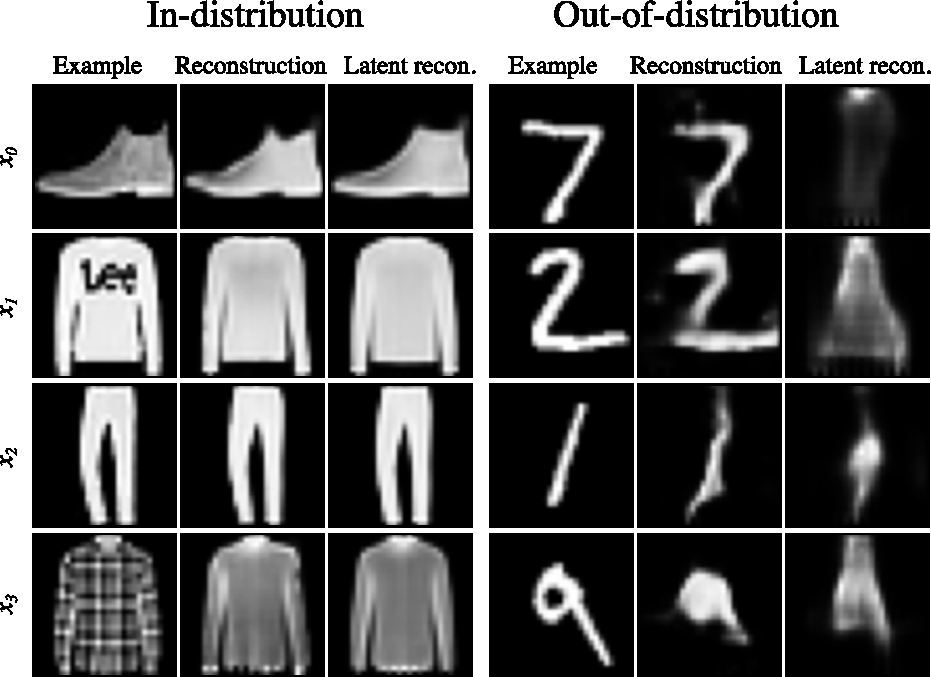
\includegraphics[width=0.7\columnwidth]{paper_hierarchical/reconstructions-front-page-4-samples-2-recons2.pdf}
    \caption[Reconstructions of a hierarchical VAE trained on FashionMNIST.]{%
        Reconstructions using a hierarchical VAE trained on FashionMNIST.
        Reconstruction quality of OOD data is comparable to in-distribution data, resulting in high likelihoods and poor OOD discrimination.
        By sampling the $k$ bottom-most latent variables from the conditional prior distribution $p(\zb_{\geq l}|\zb_{>l})$ (latent reconstructions) instead of the approximate posterior $q(\zb_{>l}|\zb_{<l})$, the model reconstructs from the training distribution resulting in lower $p(\xb|\zb)$ for OOD data.
    }
    \label{fig_hierarchical:reconstructions-fashionmnist}
\end{figure}
% First paragraph: Explains why OOD detection is important in a broad perspective
The reliability and safety of machine learning systems applied in the real-world is contingent on the ability to detect when an input is different from the training distribution. %, an anomaly.
Supervised classifiers built as deep neural networks are well-known to misclassify such \textit{out-of-distribution} (OOD) inputs to known classes with high confidence \cite{goodfellow_explaining_2015, nguyen_deep_2015}.
Several approaches have been suggested to equip deep classifiers with OOD detection capabilities \cite{hendrycks_baseline_2017, lakshminarayanan_simple_2017, hendrycks_deep_2019, devries_learning_2018}.
% However, such methods are inherently supervised and require in-distribution labels or examples of OOD data from an a priori known distribution which limit their applicability.
But, such methods are inherently supervised and require in-distribution labels or examples of OOD data limiting their applicability and generality.

% Second paragraph: Outline deep generative modeling approach and their failure
Unsupervised generative models that estimate an explicit likelihood should understand what it means to be in- and out-of-distribution without requiring labels or examples of OOD data.
By directly modeling the training distribution, such models are expected to assign low likelihoods to OOD data as it originates from regions of little or no support under the learned density \cite{bishop_novelty_1994}.
Recent advances in deep generative models \cite{kingma_autoencoding_2014, rezende_stochastic_2014, oord_pixel_2016, salimans_pixelcnn_2017, kingma_glow_2018} have enabled learning high quality generative models on complex data such as natural images, sequences including audio \cite{oord_wavenet_2016} and graphs \cite{kipf_variational_2016}.
However, recent observations have brought into question the quality of the learned density estimates by showing that they often assign higher likelihoods to OOD data than to in-distribution data \cite{nalisnick_deep_2019, choi_waic_2019}.
Many complex data distributions can be explained to a large degree by low-level features, e.g. edges in images.
However, such features do not explain high-level semantics of the data and may inhibit OOD detection \cite{ren_likelihood_2019, nalisnick_deep_2019}

\textbf{In this paper}, we examine the failure cases of deep generative models on OOD detection tasks within the context of hierarchical VAEs, and make the following contributions:
\begin{itemize}
    \item[(i)] We provide evidence that the root cause of OOD failures is that learned low-level features generalize well across datasets and dominate the estimated likelihoods.
    \item[(ii)] We then propose a fast, scalable, and fully unsupervised likelihood-ratio score for OOD detection that is explicitly developed to ensure that data should be in-distribution across all feature levels, which prevents the low-level features from dominating.
    \item[(iii)] With the likelihood-ratio score, we demonstrate state-of-the-art performance across a wide range of known OOD failure cases.
\end{itemize}


\section{Why does OOD detection fail?}\label{sec_paper_hierarchical:why-does-ood-fail}
\begin{figure}[t]
    \centering
    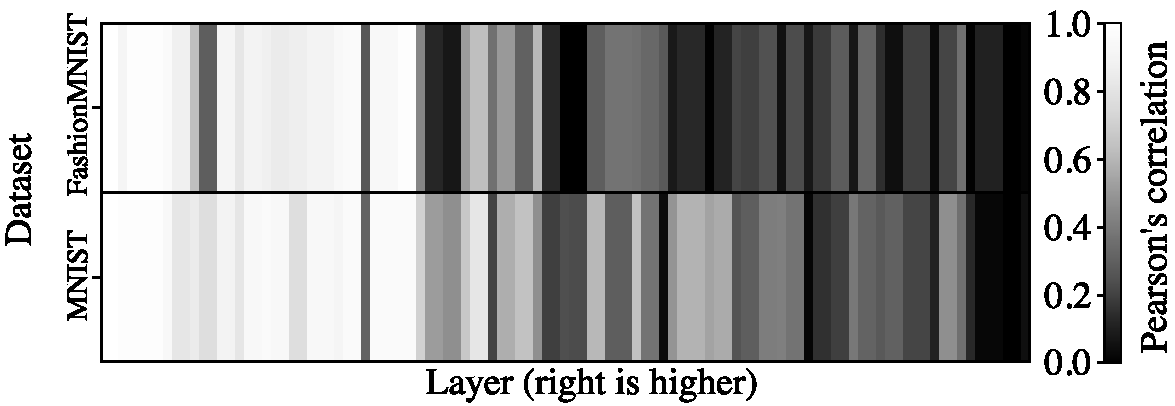
\includegraphics[width=1\columnwidth]{paper_hierarchical/feature-correlation-heatmap2.pdf}
    \vspace{0mm}
    \caption[Absolute correlations between data representations in all layers of the inference network of a hierarchical VAE trained on FashionMNIST and of another trained on MNIST.]{
    Absolute correlations between data representations in all layers of the inference network of a hierarchical VAE trained on FashionMNIST and of another trained on MNIST.
    We compute the correlation between the representations of the two different models given the same data, FashionMNIST (top) and MNIST (bottom).
    %We reduce the representations to a single number by summing over all dimensions and compute the correlation between these numbers for 256 examples.
    %To reduce de-correlation due to the stochastic latent variables, we encode using the mode of the approximate posterior distributions.
    }
    \vspace{0mm}
    \label{fig_hierarchical:correlations-heatmap}
\end{figure}

The inability to detect out-of-distribution data with deep generative models is surprising.
Before the advent of deep generative models, this was not considered a major issue for probabilistic models \cite{bishop_novelty_1994}.
Is the failure due to model pathologies or something different?

Deep learning models are generally believed to form hierarchies of representations that range from low-level features to more conceptual ones related to semantics \cite{bengio_representation_2013}.
This has also been observed within deep generative models \cite{maaloe_biva_2019, child_very_2021}.
%Recent research \cite{maaloe_biva_2019, child_very_2021, vahdat_nvae_2020}, has shown that deep latent variable models are able to learn rich hierarchical representations with increasing levels of abstraction and global structure towards the top of the hierarchy.
For image data there is a trend that the low-level features are quite similar across models (edge detectors, etc.). This raises the question to what extend such features are relevant when detecting OOD data, also suggested  by \cite{nalisnick_deep_2019} and examined for Glow and PixelCNN in \cite{schirrmeister_understanding_2020}.
To investigate, we train two hierarchical VAEs (\cref{sec_paper_hierarchical:background-hie-VAE}) on FashionMNIST and MNIST, respectively, and compute the between-models correlation of the extracted features of in-distribution data and OOD data.
The result appears in \cref{fig_hierarchical:correlations-heatmap}.
We observe that features extracted in the early layers (low-level features) correlate strongly between the two models, and that this correlation drops as we get into later layers.
This suggests that low-level features do not carry much information for OOD detection.

To shed further light on the impact of semantic versus low-level features, we look at model reconstructions of images with a hierarchical VAE (\cref{fig_hierarchical:biva-reconstructions-celeba}).
To study the feature hierarchy, we replace the inference distribution with the corresponding conditional prior in the first layers of the model to see what information is lost.
We observe that as more layers rely on the prior, more details are lost.
Sunglasses, which are uncommon, are first replaced by more common glasses, and then finally disappear.
%Likewise, a long-haired man eventually becomes woman.
This suggests that as we fall back to the conditional priors of each layer, we are pushed closer to local modes of the modeled distribution.

\begin{figure}[t]
    \centering
    %\vspace{0.17cm}
    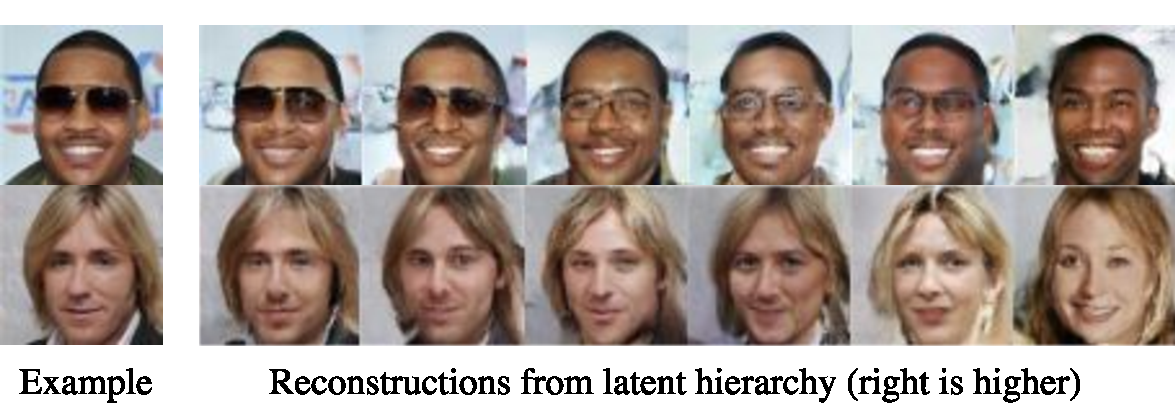
\includegraphics[width=1\columnwidth]{paper_hierarchical/biva_reconstructions.pdf}
    % https://docs.google.com/drawings/d/1UXdA3c18Oek9_env1vEB9mqOAHZ-tu0ijWmvqmapWCk/edit?usp=sharing
    \vspace{0mm}
    \caption[Reconstructions of in-distribution data (CelebA) of the BIVA model using higher latent variables.]{Reconstructions of in-distribution data (CelebA) of the BIVA model using higher latent variables  \cite{maaloe_biva_2019}.
    The higher the latent variable, the more the reconstructions fall into the mode of the learned distribution.
    It is more common to wear regular glasses than sunglasses but most common not to wear glasses at all.
    A man with long hair collapses into the mode of the more common long-haired woman.}
    \vspace{0mm}
    \label{fig_hierarchical:biva-reconstructions-celeba}
\end{figure}
Finally, we look at reconstructions of out-of-distribution data.
\cref{fig_hierarchical:reconstructions-fashionmnist} illustrates that MNIST data is surprisingly well reconstructed by a hierarchical VAE trained on FashionMNIST.
Similar results have been found elsewhere \cite{xiao_likelihood_2020}.
We repeat the previous experiment and replace inference distributions by their corresponding conditional prior, and now observe that reconstructions from higher latent layers become increasingly similar to the data on which the model was trained.
The reliance on conditional priors seems to prevent accurate reconstruction of out-of-distribution data.
Some details are lost on in-distribution data too, but the distinction between that and out-of-distribution data becomes more clear.

\textbf{These observations lead to our main hypothesis.}
The lowest latent variables in a hierarchical VAE learn generic features that can describe a wide range of data.
This enables the model to achieve high rates of compression and high likelihoods, even on out-of-distribution data as long as the learned low-level features are appropriate.
We further suggest that OOD data are in-distribution with respect to these low-level features, but not with respect to semantic ones.

\vspace{0cm}
\section{Background and related work}

\subsection{Variational autoencoders}
The variational autoencoder (VAE) \cite{kingma_autoencoding_2014, rezende_stochastic_2014} is a framework for constructing deep generative models defined by an observed variable $\mathbf{x}$ and a stochastic latent variable $\mathbf{z}$.
Typically, a neural network with parameters $\thetab$ is chosen to parameterize the generative distribution $p_\thetab(\xb,\zb)=p_\thetab(\xb|\zb)p(\zb)$, where the prior $p(\zb)$ is commonly a standard Gaussian $\mathcal{N}(\0, \Ib)$.
The true posterior $p(\zb|\xb)$ is generally not analytically tractable and is approximated by a variational distribution $q_\phib(\zb|\xb)$ parameterized via another neural network with parameters $\phib$. The approximate posterior $q_\phib(\zb|\xb)$ is most often  a diagonal covariance Gaussian.
The model parameters $\thetab$ and variational parameters $\phib$ are jointly optimized by maximizing the \textit{evidence lower bound} (ELBO),
\begin{equation}\label{eq_hierarchical:elbo}
    \log p_\thetab(\xb) \geq \mathbb{E}_{q_\phib(\zb|\xb)} \left[ \log \frac{p_\thetab(\xb,\zb)}{q_\phib(\zb|\xb)} \right] \equiv \mathcal{L}(\xb; \thetab, \phib)\ .
\end{equation}
For brevity, we will denote $\mathcal{L}(\xb; \thetab, \phib)$ as $\mathcal{L}(\xb)$ or $\mathcal{L}$. The reparameterization trick is used to backpropagate gradients through the stochastic latent variables with low variance.

The VAE is defined with a single latent variable which limits the ability to learn a high likelihood representation of complex input distributions, e.g.\ natural images.
There exists a few complementary approaches to make the VAE more flexible: (i) model a more expressive variational distribution $q_\phib(\zb|\xb)$ or prior distribution $p_\thetab(\zb)$ \cite{rezende_variational_2015, kingma_improved_2016}, (ii) model a more expressive posterior distribution $p_\thetab(\xb|\zb)$ e.g. with a autoregressive decoder \cite{oord_conditional_2016} and (iii) learn a deeper hierarchy of latent variables \cite{burda_importance_2016, sonderby_ladder_2016}.
Here, we focus on the latter.


\subsection{Hierarchical variational autoencoders}\label{sec_paper_hierarchical:background-hie-VAE}
Hierarchical VAEs are a family of probabilistic latent variable models which extends the basic VAE by introducing a hierarchy of $L$ latent variables $\zb=\zb_1, \dots, \zb_L$.
The most common generative model is defined from the top down as $p_\thetab(\xb|\zb)=p(\xb|\zb_1)p_\thetab(\zb_1|\zb_2)\cdots p_\thetab(\zb_{L-1}|\zb_L)$.
The inference model can then be defined in two ways respectively referred to as \textit{bottom-up} \cite{burda_importance_2016}
\begin{equation}
    %q_\phib(\zb|\xb)=q_\phib(\zb_1|\xb)q_\phib(\zb_2|\zb_1)\cdots q_\phib(\zb_L|\zb_{L-1})
    q_\phib(\zb|\xb) = q_\phib(\zb_1|\xb)\textstyle\prod_{i=2}^{L} q_\phib(\zb_i|\zb_{i-1})
\end{equation}
and \textit{top-down} \cite{sonderby_ladder_2016}
\begin{equation}
    % q_\phib(\zb|\xb)=q_\phib(\zb_{L}|\xb)q_\phib(\zb_{L-1}|\zb_L)\cdots q_\phib(\zb_2|\zb_1),
    q_\phib(\zb|\xb) = q_\phib(\zb_L|\xb)\textstyle\prod_{i=L-1}^{1} q_\phib(\zb_{i}|\zb_{i+1}) \ .
\end{equation}
Regardless of the choice of inference model, a hierarchical VAE is still trained using the ELBO \cref{eq_hierarchical:elbo}.

Until recently, hierarchical VAEs gave inferior likelihoods compared to state-of-the-art autoregressive \cite{ho_flow_2019} and flow-based models \cite{salimans_pixelcnn_2017}.
This was changed by \textcite{maaloe_biva_2019}, \textcite{vahdat_nvae_2020}, and \textcite{child_very_2021}, which introduced complementary methods to extend the number of latent variables to a very deep hierarchy resulting in state-of-the-art likelihood performance.

In this paper we employ a simple hierarchical VAE with bottom-up inference paths and the more powerful BIVA variant with a bidirectional (top-down and bottom-up) inference model \cite{maaloe_biva_2019}. We employ skip connections between latent variables but omit them for brevity.


\subsection{Out-of-distribution detection}\label{sec_paper_hierarchical:background-ood-detection}
% Intro to alternative scores
So far, no reliable direct likelihood-based method has been found for fully unsupervised deep generative model OOD detection.
A major line of work considers developing new scores that are more reliable than the likelihood.
This includes the \textit{typicality} test presented by \textcite{nalisnick_detecting_2019} which is an OOD detection test based on the typicality of a batch of potentially OOD examples.
This approach however requires a batch of examples from the same class (OOD or not) which limits its practical applicability.
In \textcite{ren_likelihood_2019}, the \textit{likelihood ratio} between a primary model and a background model was shown to be an effective score for OOD detection.
However, to train the background model, the in-distribution data is perturbed via a data augmentation technique that is designed with knowledge about the confounding factors between the in-distribution data and the OOD data. Furthermore, it is tuned towards high performance on a known OOD dataset.
\textcite{serra_input_2020} take a similar approach and attribute the failure to detect OOD data to the high influence of the input complexity on the likelihood and choose a generic lossless compression algorithm as the background model.
Although this method gives good results, no single best choice of compression algorithm exists for all types of OOD data, and any particular choice encodes prior knowledge about the data into the detection method.
Both these methods can be seen as correcting for low-level features of the OOD data being assigned high model likelihood by using a second model focused exclusively on these features.

Similar to these methods, the majority of the approaches to OOD detection make assumptions about the nature of the OOD data.
The assumptions encompass using labels on the in-distribution data \cite{hendrycks_baseline_2017, liang_enhancing_2018, alemi_uncertainty_2018, lee_simple_2018, lakshminarayanan_simple_2017}, examples of OOD data \cite{hendrycks_deep_2019}, augmenting in-distribution data to mimic it \cite{ren_likelihood_2019}, or assuming a certain data type \cite{serra_input_2020}.
Any of these assumptions encode implicit biases into the model about the attributes of OOD data which, in turn, might impair performance on truly unknown data examples (unknown unknowns).

% Introduce the contrast to results with VAEs
While some of these methods achieve very good results on OOD detection with autoregressive models \cite{oord_pixel_2016, salimans_pixelcnn_2017} and invertible flow-based models \cite{kingma_glow_2018}, it was recently shown that they can be much less effective for VAEs \cite{xiao_likelihood_2020} highlighting the need for a more reliable OOD score for VAEs.
Although VAEs have the same failure cases as autoregressive and flow-based models, the caveat is that the difference in the likelihood is generally not as big and reconstructions of OOD can be surprisingly good \cite{xiao_likelihood_2020}.
\textcite{xiao_likelihood_2020} alleviate this by refitting the inference network, as previously proposed by \textcite{cremer_inference_2018, mattei_refit_2018}, to a potentially OOD example and measuring the so-called \textit{likelihood regret}.
However, refitting the inference network can be computationally expensive, especially for the large hierarchical VAEs that are used to model complex data \cite{maaloe_biva_2019, vahdat_nvae_2020, child_very_2021}. Furthermore, this scales poorly to large amounts of potentially OOD examples as the optimization is done per example.

A few methods have approached OOD detection in a completely unsupervised fashion \cite{maaloe_biva_2019, choi_waic_2019, xiao_likelihood_2020}.
The work of \textcite{maaloe_biva_2019} is the most related to ours. They introduce BIVA, a deep hierarchy of stochastic latent variables with a top-down and bottom-up inference model and achieve state-of-the-art likelihood scores. 
They also provide early results indicative that a looser likelihood bound may have value in OOD detection.
In this paper, we provide an explanation of those results, and significantly improve upon them.


\section{OOD detection with hierarchical VAEs}
\subsection{A bound for semantic OOD detection}
If the lowest latent variable in the VAE hierarchy codes for a large part of the low-level features required to reconstruct the input with high accuracy, as exemplified in \cref{fig_hierarchical:reconstructions-fashionmnist}-\ref{fig_hierarchical:biva-reconstructions-celeba}, then $p_\thetab(\xb|\zb_1)$ will be high for both in- and out-of-distribution data.
Hence, any OOD detection capabilities based on the ELBO $\mathcal{L} = \mathbb{E}_{q_\phib(\zb|\xb)}[\log p_\thetab(\xb|\zb_1)] - D_{\mathrm{KL}}( q_\phib(\zb|\xb) || p(\zb))$ from \cref{eq_hierarchical:elbo} relies on the KL-term for OOD detection. For a bottom-up hierarchical VAE, the KL-term $D_{\mathrm{KL}}( q_\phib(\zb|\xb) || p(\zb))$ can be expressed by a hierarchical sum% over the hierarchy
% \begin{multline}
%     \mathcal{L}(\xb) =  \mathbb{E}_{q_\phib(\zb|\xb)} \Big[ \log p_\thetab(\xb|\zb_1) \\
%                      + \textstyle\sum_{i=1}^{L-1} \log \frac{p_\thetab(\zb_i|\zb_{i+1})}{q_\phib(\zb_i|\zb_{i-1})} 
%                      + \log \frac{p_\thetab(\zb_L)}{q_\phib(\zb_L|\zb_{L-1})} \Big] .
% \end{multline}
% \begin{multline}
%     D_{\mathrm{KL}}( q(\zb|\xb) || p(\zb)) = \\
%     \mathbb{E}_{q_\phib(\zb|\xb)} \Big[ \textstyle\sum_{i=1}^{L-1} \log \frac{p_\thetab(\zb_i|\zb_{i+1})}{q_\phib(\zb_i|\zb_{i-1})} + \log \frac{p_\thetab(\zb_L)}{q_\phib(\zb_L|\zb_{L-1})} \Big] .
% \end{multline}
\begin{equation}
    \mathbb{E}_{q_\phib(\zb|\xb)} \Big[ \textstyle\sum_{i=1}^{L-1} \log \frac{p_\thetab(\zb_i|\zb_{i+1})}{q_\phib(\zb_i|\zb_{i-1})} + \log \frac{p_\thetab(\zb_L)}{q_\phib(\zb_L|\zb_{L-1})} \Big] \ .
\end{equation}
In general, the absolute log-ratios grow with $\mathrm{dim}(\zb_i)$ as the individual log probability terms are computed by summing over the dimensionality of $\zb_i$.
This means that the value of the KL-term is dominated by terms where $\zb_i$ is high-dimensional. We refer to Appendix C for a more detailed argument.
Since hierarchical VAEs are generally constructed with a bottleneck type structure, the terms corresponding to latent variables towards the top of the hierarchy will have a vanishing influence on the value of the KL-term.
However, as the semantic information most relevant for OOD detection has a tendency to be represented in the top-most latent variables, this makes OOD detection using the regular ELBO difficult, even for state-of-the-art models.
This behavior has also been reported by \textcite{xiao_likelihood_2020}.

To shift the ELBO from primarily being based on the approximate posterior of the lowest latent variables to instead focus on the conditional prior, \textcite{maaloe_biva_2019} introduced slightly different likelihood lower bound defined as
\begin{equation}\label{eq_hierarchical:biva->k}
    \mathcal{L}^{>k} = \mathbb{E}_{p_\thetab(\zb_{\leq k}|\zb_{>k}) q_\phib(\zb_{>k}|\xb)} \left[ \log \frac{p_\thetab(\xb|\zb)p_\thetab(\zb_{>k})}{q_\phib(\zb_{>k}|\xb)} \right]
\end{equation}
where $k\in\{0,1,\dots,L\}$ (see Appendix for the derivation).
We note that $\mathcal{L}^{>0}$ is the regular ELBO (\cref{eq_hierarchical:elbo}) and that empirically we always observe that $\mathcal{L}\geq\mathcal{L}^{>k} \, \forall \, k$ although this need not hold in general.
The core idea behind this variation on the ELBO is to sample the $k$ lowest latent variables from the conditional prior $\zb_1,\dots,\zb_l \sim p_\thetab(\zb_{\leq k}|\zb_{>k})$ and only the $L-k$ highest from the approximate posterior $\zb_{k+1},\dots,\zb_L \sim q_\phib(\zb_{>k}|\xb)$.
Importantly, this has the effect that the data likelihood $p(\xb|\zb)$ is dependent on the approximate posterior through a latent variable $\zb_{k+1}$ different from $\zb_1$ for all $k \geq 1$.
Thereby, the likelihood can be evaluated with a reconstruction from each of the latent variables $\zb_k$ of the hierarchical VAE.
Hence, we can now test how well the input $\xb$ is reconstructed from each latent variable.
The notation $\mathcal{L}^{>k}$ highlights that for latent variables $\zb_{>k}$, the bound is the regular ELBO while for the latent variables $\zb_{\leq k}$, the bound is evaluated using the (conditional) prior rather than the approximate posterior as the proposal distribution.


\subsection{A likelihood-ratio score for all feature levels}
While the $\mathcal{L}^{>k}$ bound provides a score for performing semantic OOD detection, it still relies on the data space likelihood function (see equation \cref{eq_hierarchical:likelihoods-as-exact} below), which is known to be problematic for OOD detection (\cref{sec_paper_hierarchical:background-ood-detection}). To alleviate this, we phrase OOD detection as a likelihood ratio test of being \emph{semantically} in-distribution.
A standard likelihood ratio test \cite{buse_likelihood_1982} suggests to consider the ratio between the associated likelihoods, which we can approximate on a log-scale by the corresponding lower bounds $\mathcal{L}$ and $\mathcal{L}^{>k}$,
\begin{equation}\label{eq_hierarchical:llr-as-difference-in-likelihoods}
    % LLR = - 2 log(L0 / L1)
    % where L0 < L1 so log(L0 / L1) < 0 and LLR > 0
    % LLR = 2 log(L1 / L0)
    %     = 2 (log(L1) - log(L0))
    %     = 2 (ELBO - L^{>k})  % LLR^{>a,>b} where a=0
    % L1 = ELBO
    % L0 = L^{>k}
    LLR^{>k}(\xb) = \mathcal{L}(\xb) - \mathcal{L}^{>k}(\xb) \ .
\end{equation}
%This likelihood ratio contrasts the ELBO with $\mathcal{L}^{>k}$ for a variable choice of $k$.
Since, empirically, $\mathcal{L}\geq\mathcal{L}^{>k}$, the ratio is always positive as is standard for likelihood ratio tests.
A low value of $LLR^{>k}(\xb)$ means that the ELBO and $\mathcal{L}^{>k}$ are almost equally tight for the data.
On the contrary, a high value indicates that $\mathcal{L}^{>k}$ is looser on the data than the ELBO; hence, the data may be OOD.


We can gather further insights about this score if we write the regular ELBO and the $\mathcal{L}^{>k}$ bounds in the exact form that includes the intractable KL-divergence between the approximate and true posteriors,
\begin{align}
    \mathcal{L}      &= \log p_\thetab(\xb) - D_{\mathrm{KL}}\left( q_\phib(\zb|\xb) || p_\thetab(\zb|\xb)\right), \label{eq_hierarchical:likelihoods-as-exact} \\ 
    \mathcal{L}^{>k} &= \log p_\thetab(\xb) - D_{\mathrm{KL}}\left( p_\thetab(\zb_{\leq k }|\zb_{>k}) q_\phib(\zb_{>k}|\xb) || p_\thetab(\zb|\xb)\right) \nonumber \ .
\end{align}
Subtracting these cancel out the two data likelihood terms $\log p_\thetab(\xb)$ and only the KL-divergences from the approximate to the true posterior remain,
\begin{align}
    LLR^{>k}(\xb) &= - D_{\mathrm{KL}}\left( q_\phib(\zb|\xb) || p_\thetab(\zb|\xb)\right) \\
                 &\quad + D_{\mathrm{KL}}\left( p_\thetab(\zb_{\leq k}|\zb_{>k}) q_\phib(\zb_{>k}|\xb) || p_\thetab(\zb|\xb)\right) \ . \notag
\end{align}\label{eq_hierarchical:llr-as-kls}

Hence, it is clear that compared to the likelihood bound $\mathcal{L}^{>k}$, this likelihood-ratio measures divergence exclusively in the latent space whereas $\mathcal{L}^{>k}$ includes the $\log p_\thetab(\xb)$ term similar to the ELBO.
Therefore, the $LLR^{>k}$ score should be an improved method for semantic OOD detection compared to $\mathcal{L}^{>k}$.
Now, it can be noted that if we replace the regular ELBO, $\mathcal{L}$, in \cref{eq_hierarchical:likelihoods-as-exact} with the strictly tighter importance weighted bound \cite{burda_importance_2016},
\begin{equation}
    \mathcal{L}_{S} = \mathbb{E}_{q(\zb|\xb)}\left[ \log \frac{1}{N} \sum_{s=1}^{S} \frac{p(\xb, \zb^{(s)})}{q(\zb^{(s)}|\xb)} \right] \ , \label{eq_hierarchical:iw-bound}
\end{equation}
then, in the limit $S\rightarrow\infty$, we have $\mathcal{L}_{S} \rightarrow \log p_\thetab(\xb)$ and the likelihood ratio reduces to
\begin{equation}
    LLR^{>k}_{S}(\xb) \rightarrow D_{\mathrm{KL}}( p(\zb_{\leq k}|\zb_{>k}) q(\zb_{>k}|\xb) || p(\zb|\xb))
\end{equation}\label{eq_hierarchical:llr-as-kls-iwae-reduced}
which, in practice, is well-approximated for a finite $S$. We expect this importance weighted likelihood ratio to monotonically improve upon the one in \cref{eq_hierarchical:llr-as-kls} as $S$ increases and the KL-divergence in the regular ELBO that contains terms for which $\zb_i$ is high-dimensional goes to zero.


Since the scores in \cref{eq_hierarchical:llr-as-kls,eq_hierarchical:llr-as-kls-iwae-reduced} are estimated by sampling their estimators are stochastic objects with nonzero variance.
We note that $\text{Var}(\widehat{LLR}^{>k}) = \text{Var}(\hat{\mathcal{L}}) + \text{Var}(\hat{\mathcal{L}}^{>k}) - 2\, \text{Cov}(\hat{\mathcal{L}}, \hat{\mathcal{L}}^{>k})$.
Since $\log p_\thetab(\xb)$ and part of the KL divergence are identical in the expressions of $\mathcal{L}$ and $\mathcal{L}^{>k}$ we expect $\text{Cov}(\hat{\mathcal{L}}, \hat{\mathcal{L}}^{>k})$ to be positive which reduces the total variance. 
Empirical results indeed show that $\text{Var}(\widehat{LLR}^{>k})$ is larger than $\text{Var}(\hat{\mathcal{L}})$ but smaller than $\text{Var}(\hat{\mathcal{L}}^{>k})$.
%Whether this decreases the variance to below the variance of any of the two bounds, we do not know, and we believe it to be difficult to verify mathematically.
Nevertheless, the variance of the estimators is guaranteed to go to zero as the number of samples is increased.

The OOD scores considered in this research all assume that what discriminates an out-of-distribution from an in-distribution data point are semantic, high-level features. Clearly, if this is not the case and the difference instead lies in low-level statistics, the scores would likely fail. We hypothesize that a complementary bound to \cref{eq_hierarchical:biva->k}, $\mathcal{L}^{<l}$ described in Appendix E, might be useful in these cases, but leave further examination to future work.


\section{Experimental setup}

\paragraph{Tasks} We follow existing literature \cite{nalisnick_deep_2019, hendrycks_deep_2019} and evaluate our method by setting up OOD detection tasks from FashionMNIST \cite{xiao_fashionmnist_2017} to MNIST \cite{lecun_gradientbased_1998} and from CIFAR10 \cite{krizhevsky_learning_2009} to SVHN \cite{netzer_reading_2011}.
For each experiment we train our model on the train split of the former dataset and test its ability to recognize the test split of the latter dataset as OOD from the test split of the former dataset.
We use the standard train/test splits for the datasets.
More details on the datasets can be found in the Appendix.


% Our model
%\begin{wrapfigure}{R}{0.5\columnwidth}
% \begin{SCfigure}[50][t!]
\begin{figure}[t]
    %\begin{figure}
    \centering
    \resizebox{0.25\textwidth}{!}{
    \tikz{
        % inference
        % nodes
        \node[obs] (x_inf) {$\xb$};%
        \node[latent,above=.75cm of x_inf](z1_inf){$\zb_1$}; %
        \node[latent,above=.75cm of z1_inf](z2_inf){$\zb_2$}; %
        % \node[latent,above=.75cm of z2_inf](z3_inf){$\zb_3$}; %
        \node[above=of z2_inf, yshift=-1.cm] (phi) {$q_\phib(\zb|\xb)$}; 
        
        % edges
        \edge[]{x_inf}{z1_inf};
        \edge[]{z1_inf}{z2_inf};
        % \edge[]{z2_inf}{z3_inf};
        \edge[dashed, bend left]{x_inf}{z2_inf};
        % \edge[dashed, bend left]{x_inf}{z3_inf};
        
        % generative
        % nodes$
        \node[obs,right=0.75cm of x_inf] (x_gen) {$\xb$};%
        \node[latent,above=.75cm of x_gen](z1_gen){$\zb_1$}; %
        \node[latent,above=.75cm of z1_gen](z2_gen){$\zb_2$}; %
        % \node[latent,above=.75cm of z2_gen](z3_gen){$\zb_3$}; %
        \node[above=of z2_gen, yshift=-1.cm] (theta) {$p_\thetab(\xb,\zb)$}; 
        
        % edges
        % \edge[]{z3_gen}{z2_gen};
        \edge[]{z2_gen}{z1_gen};
        \edge[]{z1_gen}{x_gen};
        \edge[dashed, bend left]{z2_gen}{x_gen};
        % \edge[dashed, bend left]{z3_gen}{x_gen};
    }
    }
    \caption[Inference and generative models for a bottom-up hierarchical VAEs.]{The inference and generative models, $q_\phib$ and $p_\thetab$, for an $L=2$ layered bottom-up hierarchical VAE as the one used in our experiments.
    Dashed lines indicate deterministic skip connections which are employed in both networks. Skip connections are found to be useful for optimizing latent variable models \cite{dieng_avoiding_2019, maaloe_biva_2019}.}
    \label{fig_hierarchical:hvae-graphical-model}
    % \end{figure}
%\end{wrapfigure}
% \end{SCfigure}
\end{figure}


\paragraph{Models} For each OOD task, we train a simple bottom-up hierarchical VAE with $L$ stochastic layers which we will refer to as ``HVAE''.
To alleviate posterior collapse we include skip-connections that connect $\zb_i$ to $\zb_{i+2}$ for $i\in\{0, L-2\}$ and $\zb_0\equiv\xb$ in both the inference and generative models \cite{dieng_avoiding_2019} and employ the \textit{free bits} scheme with $\lambda=2$ \cite{kingma_improved_2016}.
We use weight-normalization \cite{salimans_weight_2016} on all weights and residual networks in the deterministic paths. 
A graphical representation of this model can be seen in \cref{fig_hierarchical:hvae-graphical-model}.
We use a Bernoulli output distribution for FashionMNIST/MNIST and a discretized mixture of logistics output distribution \cite{salimans_pixelcnn_2017} for CIFAR10/SVHN.
We use $L=3$ for grey-scale images and $L=4$ for natural images.
% For CIFAR/SVHN, we also train a BIVA model \cite{maaloe_biva_2019} with $L=10$ and similar configuration as used by the original paper\footnote{Code available at \url{github.com/larsmaaloee/BIVA} and \url{github.com/vlievin/biva-pytorch}}.
Full model details are in the Appendix.


% Baselines
\paragraph{Baselines} We group baselines into those that use prior knowledge about OOD data, ones that use labels associated with the in-distribution data and purely unsupervised approaches that do not make such assumptions.
Our method falls into the latter category.
For more information on each baseline, we refer to the original literature.


% Metrics and Evaluation
\paragraph{Evaluation} Following previous work \cite{hendrycks_baseline_2017, hendrycks_deep_2019, alemi_uncertainty_2018, ren_likelihood_2019, choi_waic_2019} we use the threshold-independent evaluation metrics of Area Under the Receiver Operator Characteristic (AUROC$\uparrow$), Area Under the Precision Recall Curve (AUPRC$\uparrow$) and False Positive Rate at 80\% true positive rate (FPR80$\downarrow$) where the arrow indicates the direction of improvement.
Note that these metrics are only computable given examples of OOD data but faced with truly OOD data (unknown unknowns), there are many ways to select thresholds to use in practice e.g.\ as the one that yields a specific tolerable false positive rate on the in-distribution test data.
To compute the metrics, we use an equal number of samples from the in-distribution and OOD datasets by including all examples in the smallest of the two sets and randomly sampling equally many from the larger. We compute the $LLR^{>k}$ score with one and $S$ importance samples denoted by $LLR^{>k}_S$.

% The value of k
\paragraph{Selection of $k$} To determine whether an example is OOD in practice, the value of $LLR^{>k}$ is computed on the in-distribution test set for all $k$ and the resulting empirical distribution is used as reference.
If for any value of $k$, the $LLR^{>k}$ score of a new input differs significantly from the empirical distribution, it is regarded OOD.
If it differs for multiple values of $k$, the value for which it differs the most is selected.
In our experiments, we consider an entire dataset at a time and report the results of $LLR^{>k}$ with the value of $k$ that yielded the highest AUROC$\uparrow$ for that dataset in a threshold-free manner.
In practice, slightly better performance may be achieved by choosing $k$ per example.
This would not exclude the use of batching in our method, since $LLR^{>k}$ is computed after the forward pass.


\section{Results}

The likelihoods for our trained models are in \cref{tab_hierarchical:bits-per-dim-ood} alongside baseline results for in-distribution and OOD data.
The main results of the paper on the OOD tasks can be seen along with comparisons to the baseline methods in \cref{tab_hierarchical:rocauc-ood}.
We note that for all our results, the value of the score ($\mathcal{L}^{>k}$ and $LLR^{>k}$) for the training and test splits of the in-distribution data was observed to have the same empirical distribution to within sampling error hence yielding an AUROC score of $\approx0.5$ as expected.
Results on additional commonly used datasets are found in Appendix G.


\begin{table}[t!]
    \centering
    \resizebox{0.8\columnwidth}{!}{%
    \begin{tabular}{lrrrrr}
        \toprule
         Method & Dataset & \multicolumn{4}{c}{Avg. bits/dim}\\
        %   & & $\log p(x)$ & $\mathcal{L}^{>k_1}$ & $\mathcal{L}^{>k_2}$ & $\mathcal{L}^{>k_3}$\\
          & & $\log p(x)$ & $\mathcal{L}^{>1}$ & $\mathcal{L}^{>2}$ & $\mathcal{L}^{>3}$\\
         \midrule
         \multicolumn{6}{c}{\textbf{Trained on FashionMNIST}} \\
         \midrule
         \multirow{2}{*}{Glow}
            & FashionMNIST & 2.96 & - & - & \\
            & MNIST & 1.83 & - & - & \\
         \multirow{2}{*}{HVAE (Ours)}
            & FashionMNIST & 0.420 & 0.476 & 0.579 & - \\
            & MNIST & 0.317 & 0.601 & 0.881 & - \\
         \midrule
         \multicolumn{6}{c}{\textbf{Trained on CIFAR10}} \\
         \midrule
         \multirow{2}{*}{Glow}
          & CIFAR10 & 3.46 & - & - & \\
          & SVHN & 2.39 & - & - & \\
         \multirow{2}{*}{HVAE (Ours)}
            & CIFAR10 & 3.74 & 17.8 & 54.3 & 75.7 \\  % log p(x) = 8010.03
            & SVHN & 2.62 & 10.2 & 64.0 & 93.9 \\
         \multirow{2}{*}{BIVA (Ours)}
          & CIFAR10 & 3.46 & 8.74 & 19.7 & 37.3 \\
          & SVHN & 2.35 & 6.62 & 25.1 & 59.0 \\
         \bottomrule
    \end{tabular}
    }
    \caption[Average bits per dimension of different datasets for generative models trained on FashionMNIST and CIFAR10.]{%
    Average bits per dimension of different datasets for models trained on FashionMNIST and CIFAR10.
    For the hierarchical models we include the $\mathcal{L}^{>k}$ bounds.
    The likelihoods of training and test splits of the in-distribution data are all cases close.
    Since we train on dynamically binarized FashionMNIST, our bits/dim are smaller than for Glow.
    As $k$ is increased for the $L^{>k}$ bound, the bound gets looser but the model eventually assigns higher likelihood to the in distribution data than to the OOD data.
    Glow refers to \textcite{kingma_glow_2018, nalisnick_deep_2019}.
    BIVA refers to our implementation of \textcite{maaloe_biva_2019}.}
    \label{tab_hierarchical:bits-per-dim-ood}
    \vspace{0mm}
\end{table}

\footnotetext{%
    \textcite{serra_input_2020} performs the best when high likelihoods are assigned to OOD data such that the overlap with in-distribution data is low.
    Performance is worse when the overlap is high, cf. \textcite[Table 1]{serra_input_2020}, as seen with complex images.}
\begin{table}[t!]
    \centering
    \resizebox*{!}{0.9\textheight}{%
    \begin{tabular}{lrrr}
        \toprule
         Method & AUROC$\uparrow$ & AUPRC$\uparrow$ & FPR80$\downarrow$ \\
         \midrule
         \multicolumn{4}{c}{\textbf{FashionMNIST (in) / MNIST (out)}} \\
         \midrule
         \multicolumn{4}{l}{\textbf{Use prior knowledge of OOD}} \\
Backgr. contrast. LR (PixelCNN) {\cite{ren_likelihood_2019}}               & $0.994$ & $0.993$ & $0.001$ \\
Backgr. contrast. LR (VAE) {\cite{choi_waic_2019}}                    & $0.924$ & - & - \\
Binary classifier {\cite{ren_likelihood_2019}}                              & $0.455$ & $0.505$ & $0.886$ \\ % 6
$p(\hat{y} | \xb)$ with OOD as noise class {\cite{ren_likelihood_2019}}     & $0.877$ & $0.871$ & $0.195$ \\ % 7
$p(\hat{y} | \xb)$ with calibration on OOD {\cite{ren_likelihood_2019}}     & $0.904$ & $0.895$ & $0.139$ \\ % 8
Input complexity ($S$, Glow) \cite{hendrycks_deep_2019}                    & $0.998$ & - & - \\
Input complexity ($S$, PixelCNN++) \cite{hendrycks_deep_2019}              & $0.967$ & - & - \\
         \multicolumn{4}{l}{\textbf{Use in-distribution data labels $y$}} \\
$p(\hat{y} | \xb)$ {\cite{ren_likelihood_2019, hendrycks_baseline_2017}}                        & $0.734$ & $0.702$ & $0.506$ \\
Entropy of $p(y | \xb)$ {\cite{ren_likelihood_2019}}                        & $0.746$ & $0.726$ & $0.448$ \\
ODIN {\cite{ren_likelihood_2019, liang_enhancing_2018}}                                       & $0.752$ & $0.763$ & $0.432$ \\
VIB \cite{alemi_uncertainty_2018, choi_waic_2019}                                          & $0.941$ & - & - \\
Mahalanobis distance, CNN {\cite{ren_likelihood_2019}}                     & $0.942$ & $0.928$ & $0.088$ \\
Mahalanobis distance, DenseNet {\cite{lee_simple_2018}}                & $0.986$ & - & - \\
Ensemble, 20 classifiers {\cite{ren_likelihood_2019, lakshminarayanan_simple_2017}}                  & $0.857$ & $0.849$ & $0.240$ \\
         \multicolumn{4}{l}{\textbf{No OOD-specific assumptions}} \\
         \multicolumn{4}{l}{\textit{- Ensembles}} \\
WAIC, 5 models, VAE {\cite{choi_waic_2019}}                          & $0.766$ & - & - \\
WAIC, 5 models, PixelCNN {\cite{ren_likelihood_2019}}                      & $0.221$ & $0.401$ & $0.911$ \\
        \multicolumn{4}{l}{\textit{- Not ensembles}} \\
Likelihood regret \cite{xiao_likelihood_2020}                               & $\mathbf{0.988}$ & - & - \\
$\mathcal{L}^{>0}$ + HVAE (ours)                    & $0.268$ & $0.363$ & $0.882$ \\
$\mathcal{L}^{>1}$ + HVAE (ours)                    & $0.593$ & $0.591$ & $0.658$ \\
$\mathcal{L}^{>2}$ + HVAE (ours)                    & $0.712$ & $0.750$ & $0.548$ \\
$LLR^{>1}$ + HVAE (ours)                            & $0.964$ & $0.961$ & $0.036$ \\
$LLR^{>1}_{250}$ + HVAE (ours)                      & $0.984$ & $\mathbf{0.984}$ & $\mathbf{0.013}$ \\
         \midrule
         \multicolumn{4}{c}{\textbf{CIFAR10 (in) / SVHN (out)}} \\
         \midrule
         \multicolumn{4}{l}{\textbf{Use prior knowledge of OOD}} \\
Backgr. contrast. LR (PixelCNN) {\cite{ren_likelihood_2019}}               & $0.930$ & $0.881$ & $0.066$ \\
Backgr. contrast. LR (VAE) {\cite{xiao_likelihood_2020}}                    & $0.265$ & - & - \\
Outlier exposure {\cite{hendrycks_deep_2019}}                              & $0.984$ & - & - \\
Input complexity ($S$, Glow) \cite{serra_input_2020}                   & $0.950$ & - & - \\
Input complexity ($S$, PixelCNN++) \cite{serra_input_2020}             & $0.929$ & - & - \\
Input complexity ($S$, HVAE) (Ours) \cite{serra_input_2020}\footnotemark & $0.833$ & $0.855$ & $0.344$ \\
         \multicolumn{4}{l}{\textbf{Use in-distribution data labels $y$}} \\
Mahalanobis distance {\cite{lee_simple_2018}}                          & $0.991$ & - & -  \\
         \multicolumn{4}{l}{\textbf{No OOD-specific assumptions}} \\
         \multicolumn{4}{l}{\textit{- Ensembles}} \\
WAIC, 5 models, Glow {\cite{choi_waic_2019}}                          & $1.000$ & - & - \\
WAIC, 5 models, PixelCNN {\cite{ren_likelihood_2019}}                      & $0.628$ & $0.616$ & $0.657$ \\
         \multicolumn{4}{l}{\textit{- Not ensembles}} \\
Likelihood regret \cite{xiao_likelihood_2020}                               & $0.875$ & - & - \\
$LLR^{>2}$ + HVAE (ours)                            & $0.811$ & $0.837$ & $0.394$ \\
$LLR^{>2}$ + BIVA (ours)                            & $\mathbf{0.891}$ & $\mathbf{0.875}$ & $\mathbf{0.172}$ \\
         \bottomrule
    \end{tabular}%
    }
    \caption[AUROC, AUPRC, and FPR80 of generative models for OOD detection (MNIST/FashionMNIST and SVHN/CIFAR10).]{%
        AUROC$\uparrow$, AUPRC$\uparrow$ and FPR80$\downarrow$ for OOD detection for a FashionMNIST model using scores on the FashionMNIST test set as reference. We bold the best results within the "No OOD-specific assumptions" group since we only compare directly to those.
        HVAE (ours) refers to our hierarchical bottom-up VAE.
        BIVA (ours) refers to our implementation of the hierarchical BIVA model \cite{maaloe_biva_2019}.
    }
    \label{tab_hierarchical:rocauc-ood}
\end{table}


\subsection{Likelihood-based OOD detection}
% \begin{sidewaysfigure}
\begin{figure}
    %\captionstyle{centerlast}
    \centering
    \begin{subfigure}[l]{0.48\columnwidth}
        \centering
        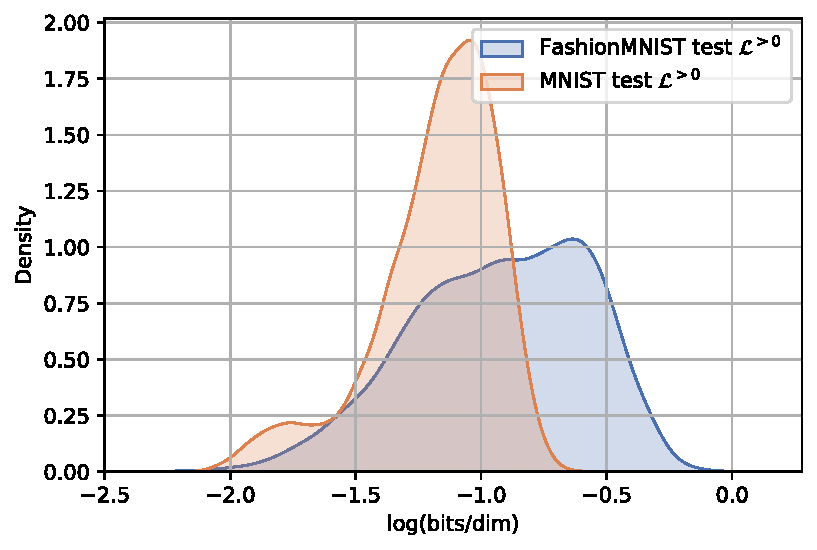
\includegraphics[width=1\columnwidth]{paper_hierarchical/densities-FashionMNIST-test-MNIST-test-bpp-k-0_sohau.pdf}
        \caption{}
        \label{fig_hierarchical:FMNIST-elbo-k0}
    \end{subfigure}
    % \hfill
    \begin{subfigure}[c]{0.48\columnwidth}
        \centering
        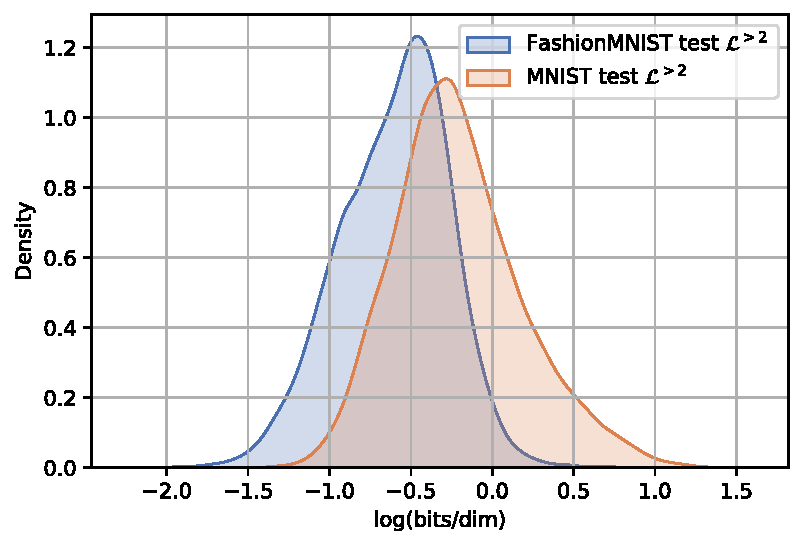
\includegraphics[width=1\columnwidth]{paper_hierarchical/densities-FashionMNIST-test-MNIST-test-bpp-k-2_sohau.pdf}
        \caption{}
        \label{fig_hierarchical:FMNIST-elbo-k2}
    \end{subfigure}
    % \hfill
    \begin{subfigure}[r]{0.48\columnwidth}
        \centering
        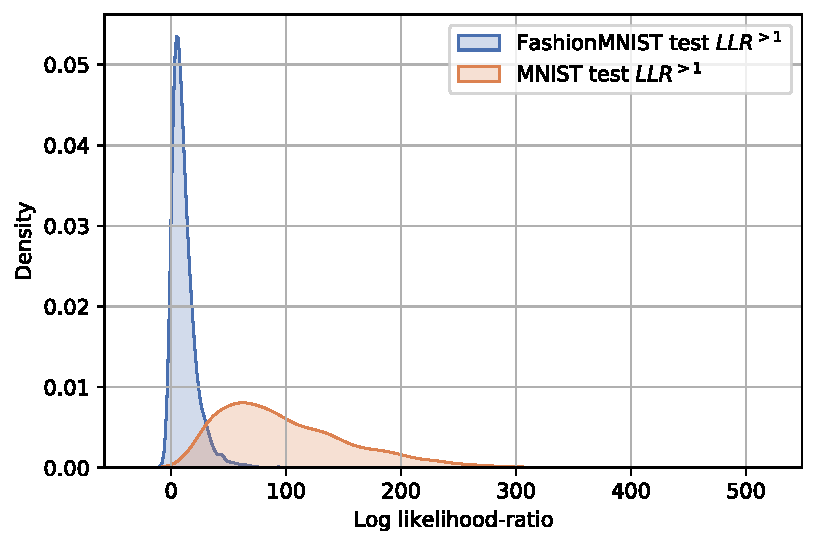
\includegraphics[width=1\columnwidth]{paper_hierarchical/densities-FashionMNIST-test-MNIST-test-LLR-0-1_sohau.pdf}
        \caption{}
        \label{fig_hierarchical:FMNIST-llr}
    \end{subfigure}
    \caption[Empirical densities of FashionMNIST (in-distribution) and MNIST (OOD) using the raw likelihood and $\mathcal{L}^{>2}$ bound.]{%
    Empirical densities of FashionMNIST (in-distribution) and MNIST (OOD) using the raw likelihood \subref{fig_hierarchical:FMNIST-elbo-k0}, the $\mathcal{L}^{>2}$ bound \subref{fig_hierarchical:FMNIST-elbo-k2} and the $LLR^{>1}$ score \subref{fig_hierarchical:FMNIST-llr}. All densities are computed using the HVAE model.
    For the regular likelihood MNIST is very clearly more likely on average than the FashionMNIST test data while with the $\mathcal{L}^{>2}$ bound separation is better but significant overlap remains.
    The $LLR^{>1}$ provides a high degree of separation. Likelihoods are reported in units of the natural log of the number of bits per dimension.
    }
    \label{fig_hierarchical:FMNIST-ood-densities}
\end{figure}
% \end{sidewaysfigure}

We first report the results of the different variations of the $\mathcal{L}^{>k}$ bound for OOD detection. 
We reconfirm the results of \textcite{nalisnick_deep_2019} by observing that our hierarchical latent variable models also assign higher $\mathcal{L}^{>0}$ to the OOD dataset in the FashionMNIST/MNIST and CIFAR10/SVHN cases resulting in an AUROC$\uparrow$ inferior to random (\cref{tab_hierarchical:rocauc-ood}).
Switching the in-distribution data for the OOD data in both cases result in correctly detecting the OOD data; an asymmetry also reported by \textcite{nalisnick_deep_2019}.
\cref{fig_hierarchical:FMNIST-elbo-k0} shows the density of $\mathcal{L}^{>0}$ in bits per dimension \cite{theis_note_2016} by the model trained on FashionMNIST when evaluated on the FashionMNIST and MNIST test sets.
We observe a high degree of overlap, with less separation of the OOD data compared to similar results of autoregressive and flow-based models, like \textcite{xiao_likelihood_2020}.


We then evaluate the looser $\mathcal{L}^{>k}$ \cref{eq_hierarchical:biva->k} for $k\in\{1,L\}$.
\cref{fig_hierarchical:FMNIST-elbo-k2} shows the result for $\mathcal{L}^{>2}$, which yielded the highest AUCROC$\uparrow$, only slightly better than random.
Like \textcite{maaloe_biva_2019}, we see that increasing the value of $k$ generally leads to improved OOD detection.
However, we also observe that the two empirical distributions never cease to overlap.
Importantly, depending on the OOD dataset, the amount of remaining overlap can be high which limits the discriminatory power of the likelihood-based $\mathcal{L}^{>k}$ bound.
This is in-line with the pathological behavior of the raw likelihood of latent variable models when used for OOD detection \cite{xiao_likelihood_2020}.
Since a high degree of overlap also seems present in \textcite{maaloe_biva_2019}, and we see the same problem for our BIVA model trained on CIFAR10, we do not expect this to be due to the less expressive HVAE.


\subsection{Likelihood-ratio-based OOD detection}
\begin{figure}
    \centering
    \begin{subfigure}[l]{0.495\columnwidth}
        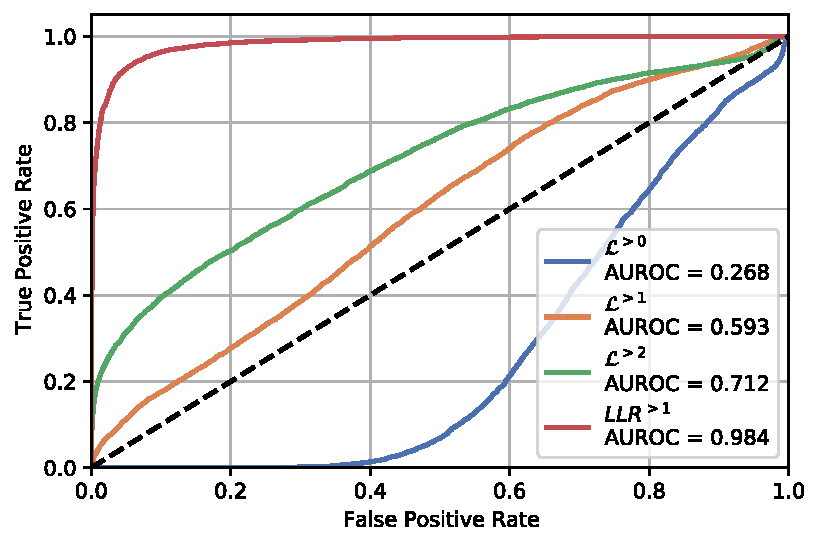
\includegraphics[width=1\columnwidth]{paper_hierarchical/roc-FashionMNIST-test-MNIST-test-ll-and-llr-IW250_sohau.pdf}
        \caption{}
        % \caption{ROC curves with AUROC score for detecting MNIST as OOD with the HVAE model trained on FashionMNIST.
        % A ROC curve is plotted for each of the $\mathcal{L}^{>k}$ bounds including the ELBO along with one for the best-performing log likelihood-ratio $LLR^{>1}$.}
        \label{fig_hierarchical:FMNIST-roc-llr}
    \end{subfigure}
    \hfill
    \begin{subfigure}[r]{0.495\columnwidth}
        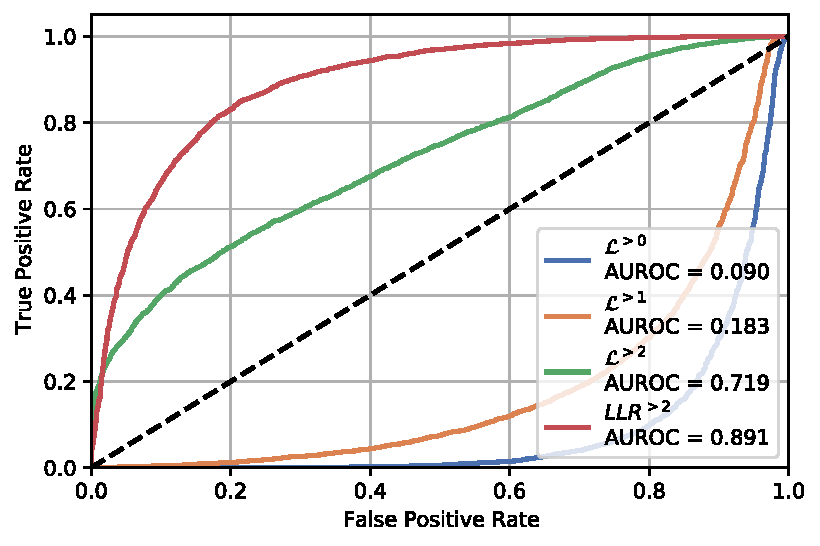
\includegraphics[width=1\columnwidth]{paper_hierarchical/roc-biva-CIFAR10-SVHN-ll-and-llr_sohau.pdf}
        \caption{}
        % \caption{ROC curves with AUROC score for detecting SVHN as OOD with the BIVA model trained on CIFAR10.
        % A ROC curve is plotted for each of the $\mathcal{L}^{>k}$ bounds including the ELBO along with one for the best-performing log likelihood-ratio $LLR^{>2}$.}
        \label{fig_hierarchical:CIFAR10-roc-llr}
    \end{subfigure}
    \caption[ROC curves for out of distribution detection (MNIST/FashionMNIST and SVHN/CIFAR10).]{%
        ROC curves with AUROC score for detecting \subref{fig_hierarchical:FMNIST-roc-llr} MNIST as OOD with the HVAE model trained on FashionMNIST and \subref{fig_hierarchical:CIFAR10-roc-llr} SVHN as OOD with the BIVA model trained on CIFAR10. 
        A ROC curve is plotted for each of the $\mathcal{L}^{>k}$ bounds including the ELBO along with one for the best-performing log likelihood-ratio $LLR^{>1}$.
    }
\end{figure}
We now move to the likelihood ratio-based score.
We find that $LLR^{>k}$ separates the OOD MNIST data from in-distribution FashionMNIST to a higher degree than the likelihood estimates as can be seen by the empirical densities of the score in \cref{fig_hierarchical:FMNIST-llr}.
We note that the likelihood ratio between the ELBO and the $\mathcal{L}^{>k}$ bound provides the highest degree of separation of MNIST and FashionMNIST as measured by the AUROC$\uparrow$ for $k=1$ smaller than $L$.
This is not surprising since the value of $k$ that provides the maximal separation to the reference in-distribution dataset need not be the one for which $\mathcal{LLR}^{>k}$ is overall maximal for the OOD dataset.
We also visualize the ROC curves resulting from using the $LLR^{>k}$ score for OOD detection on both FashionMNIST/MNIST and CIFAR10/SVHN and compare it to the ROC curves resulting from the different $\mathcal{L}^{>k}$ bounds in Figures \ref{fig_hierarchical:FMNIST-roc-llr} and \ref{fig_hierarchical:CIFAR10-roc-llr}, respectively.
On both datasets we see significantly better discriminatory performance when using the $LLR^{>k}$ score.

\cref{tab_hierarchical:rocauc-ood} shows that BIVA improves upon the HVAE model for OOD detection on CIFAR while \cref{tab_hierarchical:bits-per-dim-ood} shows that the BIVA model also improves upon the HVAE in terms of likelihood.
We hypothesize that models larger than our implementation of BIVA, with better likelihood scores may perform even better \cite{maaloe_biva_2019, vahdat_nvae_2020, child_very_2021}.


\subsection{Comparison to baselines}
\paragraph{Performance} \cref{tab_hierarchical:rocauc-ood} summarize our results compared to baselines based on the commonly used AUROC$\uparrow$, AUPRC$\uparrow$ and FPR80$\downarrow$ metrics.
Our method outperforms other generative model-based methods such as WAIC \cite{choi_waic_2019} with Glow model and performs similarly to the likelihood regret method of \cite{xiao_likelihood_2020}.
Furthermore, our method performs similarly to the background constrative likelihood ratio method of \textcite{ren_likelihood_2019} on FashionMNIST/MNIST but contrary to the failure of that method on CIFAR10/SVHN reported by \cite{xiao_likelihood_2020}, our method performs very well on this task too.
Our approach outperforms all supervised approaches that use in-distribution labels or synthetic examples of OOD data derived from the in-distribution data including ODIN \cite{liang_enhancing_2018} and the predictive distribution of a classifier $p(\hat{y}|\xb)$ trained and evaluated in various ways (see \textcite{ren_likelihood_2019}).

\paragraph{Runtime} For a full evaluation of a single example across all feature levels of a model with $L$ stochastic layers, our method requires $L-1$ forward passes through the inference and generative networks as well as computing the likelihood ratio, of which the forward passes are dominant.
For a typical forward pass that is linear in the input dimensionality, $D$, and the number of stochastic layers, $L$, this amounts to computation of $\mathcal{O}(DL)$.
Compared to some related work that either requires an $M>1$ sized batch of inputs of which either all or none are OOD \cite{nalisnick_detecting_2019} or cannot be applied to batches due to the required per-example optimization \cite{xiao_likelihood_2020}, our method additionally is applicable to batches of any size that may consist of both OOD and in-distribution examples which provides drastic speed-ups via vectorization and parallelization.
Furthermore, the method of \textcite{xiao_fashionmnist_2017} requires refitting the inference network of a VAE which can be computationally demanding.
Compared to the likelihood ratio proposed in \textcite{ren_likelihood_2019}, our method requires training only a single model on a single dataset.


\section{Discussion}
Deep generative models are state-of-the-art density estimators, but the OOD failures reported in recent years have raised concerns about the limitations of such density estimates. Recent work on improving OOD detection has largely sidestepped this concern by relying on additional assumptions that strictly should not be needed for models with explicit likelihoods.
While the engineering challenge of building reliable OOD detection schemes is important, it is of more fundamental importance to understand \emph{why} the naive likelihood test fails.
We have provided evidence that low-level features of the neural nets dominate the likelihood, which gives a \emph{cause} to the \emph{why}.
The fact that a simple score for measuring the importance of semantic features yield state-of-the-art results on OOD detection without access to additional information gives validity to our hypothesis.

The findings from, amongst others, \textcite{nalisnick_deep_2019, serra_input_2020} have a clear relation to information theory and compression. 
Semantically complex in-distribution data yields models with diverse low-level feature sets that enable generalization across datasets.
Simpler datasets can only yield models with less diverse low-level feature sets compared to complex training data.
Hence, there can be an asymmetry where the likelihoods of simple OOD data can be high for a model trained on complex data, but not the other way around.
Loosely put, the minimal number of bits required to losslessly compress data sampled from some distribution is the entropy of the generating process \cite{shannon_mathematical_1948, mackay_information_2003}.
\textcite{townsend_practical_2019} recently showed that VAEs can be used for lossless compression at rates superior to more generic algorithms.

We also note that since the hierarchical VAE is a probabilistic graphical latent variable model, it lends itself very naturally to manipulation at the feature level \cite{kingma_semi-supervised_2014, maaloe_auxiliary_2016, maaloe_semi-supervised_2017}.
This property sets it apart from other generative models that do not explicitly define such a hierarchy of features.
This in turn enables reliable OOD detection with our methodology while making no explicit assumptions about the nature of OOD data and only using a single model. This has not been achieved with autoregressive or flow-based models.

\section{Conclusion}
In this paper we study unsupervised out-of-distribution detection using hierarchical variational autoencoders.
We provide evidence that highly generalizeable low-level features contribute greatly to estimated likelihoods resulting in poor OOD detection performance.
We proceed to develop a likelihood-ratio based score for OOD detection and define it to explicitly ensure that data must be in-distribution across all feature levels to be regarded in-distribution.
This ratio is mathematically shown to perform OOD detection in the latent space of the model, removing the reliance on the troublesome input-space likelihood.
We point out that contrary to much recent literature on OOD detection, our approach is fully unsupervised and does not make assumptions about the nature of OOD data.
Finally, we demonstrate state-of-the-art performance on a wide range of OOD failure cases.


\section*{Acknowledgements}
This research was partially funded by the Innovation Fund Denmark via the Industrial PhD Programme (grant no.\@ 0153-00167B). JF and SH were funded in part by the Novo Nordisk Foundation (grant no.\@ NNF20OC0062606) via the Center for Basic Machine Learning Research in Life Science (MLLS, \hyperlink{https://www.mlls.dk}{https://www.mlls.dk}). JF was further funded by the Novo Nordisk Foundation (grant no.\@ NNF20OC0065611) and the Independent Research Fund Denmark (grant no.\@ 9131-00082B). SH was further funded by VILLUM FONDEN (15334) and the European Research Council (ERC) under the European Union’s Horizon 2020 research and innovation programme (grant agreement no. 757360).

% }
%!TEX root = ../thesis.tex

\chapter[model-agnostic out-of-distribution detection using combined statistical tests]{Model-Agnostic Out-of-Distribution Detection Using Combined Statistical Tests}
\label{chp:paper-modelagnostic}
\ifthenelse{\equal{\skippapers}{true}}{}{

\section*{Abstract}
We present simple methods for out-of-distribution detection using a trained generative model. These techniques, based on classical statistical tests, are model-agnostic in the sense that they can be applied to any differentiable generative model. The idea is to combine a classical parametric test (Rao's score test) with the recently introduced typicality test. These two test statistics are both theoretically well-founded and exploit different sources of information based on the likelihood for the typicality test and its gradient for the score test. We show that combining them using Fisher's method overall leads to a more accurate out-of-distribution test. We also discuss the benefits of casting out-of-distribution detection as a statistical testing problem, noting in particular that false positive rate control can be valuable for practical out-of-distribution detection. Despite their simplicity and generality, these methods can be competitive with model-specific out-of-distribution detection algorithms without any assumptions on the out-distribution. %out-of-distribution data.\looseness=-1

\section{Introduction}

The ability to recognize when data are anomalous, i.e. if they originate from a distribution different from that of the training data, is a necessary property for machine learning models for safe and reliable applications in the real world. Historically, \textcite{bishop_novelty_1994} proposed to use a one-sided threshold on the log-likelihoods of a learned model as a decision rule to identify outliers in a dataset. However, recently, \textcite{nalisnick_deep_2019,hendrycks_deep_2019} showed that state-of-the-art deep generative models (DGMs) failed in this task, assigning higher a likelihood to out-of-distribution (OOD) data than in"-distribution data. Most of the recent works focused on proposing new test statistics to alleviate the problem of using the plain likelihood, see \cref{sec_modelagnostic:related_works} for details.

We believe that OOD detection should be formulated as statistical hypothesis testing \parencite{nalisnick_detecting_2019, ahmadian_likelihoodfree_2021, haroush_statistical_2021}. Since the power of a single test depends on the out-distribution \parencite{zhang_understanding_2021}, we propose to approach this problem by using a combination of multiple statistical tests. %While this does not solve completely the problem, because the power of the combined tests will also depend on the out-distribution, we think that we can get better performance than using a single-statistics especially in situations where one statistic fails. 
While the power of the combined test also depends on the out-distribution, we hypothesize that the combined test empirically will perform better, especially in situations where one of the statistics fails.
%
%Furthermore, the use of the statistical testing framework, allows us to correct for the multiple comparisons problem when identifying outliers in a dataset by controlling the number of type I errors through the false discovery rate (FDR).
Furthermore, the use of the statistical testing framework has several advantages. Since we obtain a $p$-value, it is more natural deciding on a threshold as this corresponds to the significance level. In addition to that, it also allows us to correct for the multiple comparisons problem when identifying outliers in a dataset by controlling the number of Type I errors through the false discovery rate (FDR).

In summary, our contributions are the following:
\begin{itemize}
    \item We illustrate the benefits of combining multiple statistical tests to perform OOD detection with DGMs using well-established methods. This allows for a proper decision procedure to control the FDR in a real outlier detection setting.
    \item We revisit some proposed detection scores and highlight their alternative formulation as classical significance tests.
    \item Empirically we show the complementarity of the typicality and the score statistics and that their combination leads to a robust score for anomaly detection. %We evaluate our proposed method with two PixelCNN++ \textcite{salimans_pixelcnn_2017}, two Glow models \textcite{kingma_glow_2018} and one Hierarchical-VAE (HVAE)\textcite{kingma_autoencoding_2014}.
\end{itemize}
%

%% %%%%%%%%%%%%%%%%%%%%%%%%%%%%%%%%%%  SECTION 2   %%%%%%%%%%%%%%%%%%%%%%%%%%%%%%%%%%
\section{Using statistical tests for out-of-distribution detection}

We consider some data of interest that live in a space $\mathcal{X}$. Assume that we have a curated dataset $x_1,\ldots,x_m$, i.e.\@ there are no outliers, and we are interested in understanding if some new data $\tilde{x}_1,\ldots,\tilde{x}_n$ are collectively anomalies. In other words, we wonder whether or not $\tilde{x}_1,\ldots,\tilde{x}_n$ are likely to come from the same distribution that generated our curated dataset. We present in this section two different approaches for doing out-of-distribution detection using statistical tests: one based on classical parametric tests and one based on maximum mean discrepancy. A convenient property of the tests we consider is that they are all one-sided, which means we can expect them to be larger when the data are more likely to be OOD. This allows us to compute $p$-values by simply using the empirical CDF, which is hyperparameter-free.

Note that in this problem formulation, the case $n=1$ corresponds to the situation where we need to decide if a \emph{single} data point is out-of-distribution. This hardest setting will be of particular interest, and this is also the main focus of recent work, see \cref{sec_modelagnostic:related_works}.

\subsection{Parametric tests for out-of-distribution detection}\label{sec_modelagnostic:parametric}
The typical approach is to consider a parametric family $(p_\theta)_{\theta \in  \Theta}$ of probability densities over $\mathcal{X}$ and learn a suitable $\theta_0 \in  \Theta$ using any inference technique, for example maximum likelihood, and the clean data $x_1,\ldots,x_m$. Depending on the input domain, $(p_\theta)_{\theta \in  \Theta}$ could be composed of DGMs (in that case, $\theta$ would be neural network weights) or Gaussian mixture models (in that case, $\theta$ would be composed of means, covariances, and proportions). The question we wish to answer may then be phrased: \emph{is $p_{\theta_0}$ an appropriate model for $\tilde{x}_1,\ldots,\tilde{x}_n$?}
%We consider some data of interest that live in a space $\mathcal{X}$. We are given a parametric family $(p_\theta)_{\theta \in  \Theta}$ of probability densities over $\mathcal{X}$. For instance $(p_\theta)_{\theta \in  \Theta}$ could be composed of DGMs (in that case, $\theta$ would be neural network weights) or Gaussian mixture models (in that case, $\theta$ would be composed of means, covariances, and proportions).
%
%Upon analysis of an initial, in-distribution training dataset, we learn a suitable $\theta_0 \in  \Theta $ using any inference technique, for example maximum likelihood. We are now given additional data points $\tilde{x}_1,\ldots,\tilde{x}_n$ and wonder whether or not they are likely to come from the same distribution that generated our training dataset. The case $n=1$ corresponds to the case where we need to decide if a \emph{single} data point is out-of-distribution; this hardest setting will be of particular interest.
%The question we wish to answer may then be phrased: \emph{is $p_{\theta_0}$ an appropriate model for $\tilde{x}_1,\ldots,\tilde{x}_n$?}

We choose to formalize this problem as a \emph{parametric test} whose alternative hypothesis is that $\tilde{x}$ is \emph{out-of-distribution}. More specifically, if we assume that $\tilde{x}_1,\ldots,\tilde{x}_n \sim_{\textup{i.i.d.}} p_{\tilde{\theta}}$ for some unknown $\tilde{\theta} \in \Theta$, we wish to test $\mathcal{H}_0 : \tilde{\theta} = \theta_0$ against $\mathcal{H} : \tilde{\theta} \neq \theta_0$, where the alternative hypothesis $\mathcal{H}$ is that the test points are OOD.
%we wish to test $\mathcal{H}_\textup{id} : \tilde{\theta} = \theta_0$ against $\mathcal{H}_\textup{ood} : \tilde{\theta} \neq \theta_0$.

Many tests have been proposed for this purpose. The three most famous are the \emph{likelihood ratio test} of \textcite{neyman_use_1928}, Rao's \citeyearpar{rao_large_1948} \emph{score test},
%(also called \emph{Lagrange multiplier test}, mostly by econometricians),
and \emph{the Wald test} \parencite{wald_tests_1943}. These three classics are nicely reviewed by \textcite{buse_likelihood_1982} or by \textcite{rao_score_2005}, who called them the ``Holy Trinity''. A recent and interesting one is the \emph{gradient test} of \textcite{terrell_gradient_2002}, which is reviewed in great detail in Lemonte's \citeyearpar{lemonte_gradient_2016} monograph.

Let us review the statistics of these four tests:
\begin{itemize}
    \item likelihood ratio statistic is $S_{LR} = 2 ( \ell ( \hat{\theta}) -\ell ( \theta_0))$,
    \item Wald statistic is $S_{W} = (\hat{\theta} - \theta_0)^T I(\hat{\theta}) (\hat{\theta} - \theta_0)$,
    \item score statistic is $S_{S} = \nabla \ell ( \theta_0)^T I(\theta_0)^{-1}  \nabla \ell ( \theta_0)$,
    \item gradient statistic is $S_{G} = \nabla \ell ( \theta_0)^T (\hat{\theta} - \theta_0)$,
\end{itemize}
where $ \ell ( \theta) = \log p_\theta (\tilde{x}_1,\ldots,\tilde{x}_n)$ is the likelihood function, 
$I({\theta}) = \mathbb{E}_{p_\theta}[\nabla \ell ( \theta)\nabla \ell ( \theta)^T]$ is the Fisher information matrix (FIM), and $ \hat{\theta} \in \arg\max_{\theta \in \Theta} \ell ( \theta)$.

The likelihood ratio statistic, the Wald statistic and the gradient statistic all require to fit a model on the additional data points $\tilde{x}_1,\ldots,\tilde{x}_n$ in order to compute either $\ell(\hat{\theta})$ or $\hat{\theta}$. 
%
%In our setting, if we want to use one of those statistics as an OOD score for a single example, we should fit a DGM on that single data point. \textcite{xiao_likelihood_2020} try to do that in the context of VAEs by re-fitting only the inference network, or encoder, of a VAE to every single additional example. This is the typical thing to do when dealing with out-of-sample data in VAEs, as argued by \textcite{mattei2018refit, cremer2018inference}. 
In our setting, if we want to use one of those statistics as an OOD score for a single example, we should fit a DGM on that single data point. \textcite{xiao_likelihood_2020} did this for a variational autoencoder (VAE, \citealp{kingma_autoencoding_2014,rezende_stochastic_2014}) by only re-fitting inference network (or encoder) to the additional example, which is a typical approach to dealing with out-of-sample data in VAEs, as argued by \textcite{cremer_inference_2018} and \textcite{mattei_refit_2018}.
However, much of the recent works in the literature \parencite{ren_likelihood_2019, schirrmeister_understanding_2020, serra_input_2020} mainly focus on deriving different versions of what they call a likelihood ratio statistic.

%In our setting, if we want to use one of those statistics as an OOD score for a single example, we should fit a DGM on that single data point, which barely sounds serious. Most of the recent works in the literature mainly focus on deriving different versions of what they call a likelihood ratio statistic. Among those that trained a likelihood-based model on $\tilde{x}_1,\ldots,\tilde{x}_n$, we note that the work by \textcite{xiao_likelihood_2020} is the one that is closer to the real definition of the likelihood ratio statistic given by \textcite{neyman_use_1928}. Indeed, they propose to compute $\ell(\hat{\theta})$ by refitting the inference network of a VAE to every single additional example as proposed in \textcite{mattei2018refit, cremer2018inference}. 
%While a similar approach could potentially be used to compute also the gradient statistic and the Wald statistic, this will be possible only for a VAE model. 
%
We tried to derive a general way to compute both the Wald statistic and the gradient statistic, by computing $ \hat{\theta}$ with a few steps of a gradient-based optimization algorithm initialized at $ \theta_0$, but this resulted in a very unstable update leading to computational issues (results not shown). Therefore, in this work we focus on studying the relevance of the score statistic for performing out-of-distribution detection since it is the only statistic that does not require fitting an additional model to the OOD data.


\subsection{Maximum mean discrepancy for out-of-distribution detection}\label{sec_modelagnostic:MMD}
Another way of approaching out-of-distribution detection from a testing perspective is through a \emph{two-sample test}. Denoting $p_\textup{data}$ the true training data distribution, the goal is to test $\mathcal{H}_0: \tilde{x}_1,\ldots,\tilde{x}_n \sim p_\textup{data}$ against $\mathcal{H}: \tilde{x}_1,\ldots,\tilde{x}_n \not\sim p_\textup{data}$, where the alternative hypothesis $\mathcal{H}$ again is that the test points are OOD.

A popular way of building statistics for two-sample tests is to use a measure of distance between $p_\textup{data}$ and the distribution of $\tilde{x}_1,\ldots,\tilde{x}_n$. The key idea here will be to use the trained generative model to build this measure of distance. To this end, we will use the \emph{maximum mean discrepancy (MMD)} of \textcite{gretton_kernel_2012}, which is a kernel-based measure of distance. Then, $p_\theta$ will be used to specify an appropriate kernel.

More specifically, given a kernel whose feature map is $\Phi : \mathcal{X} \to \mathcal{H}$, the MMD between two distributions $P$ and $Q$ over $\mathcal{X}$ is defined as
\begin{equation}
    \textup{MMD}_\Phi(P,Q) = \| E_{X\sim P}[\Phi(X)] - E_{Y\sim Q}[\Phi(Y)] \|_\mathcal{H}. \hspace{-.1em}
\end{equation}
In our context, the test statistics will be of the form
\begin{equation}
    \label{eq_modelagnostic:mmd}
    \textup{MMD}_\Phi\left(\frac{1}{m}\sum_{i=1}^{m} x_i,\frac{1}{n}\sum_{i=1}^n \tilde{x}_i\right) = \left\|\frac{1}{m}\sum_{i=1}^{m} \Phi(x_i) -  \frac{1}{n}\sum_{i=1}^{n} \Phi(\tilde{x}_i)\right\|_\mathcal{H},
\end{equation}
where $\Phi$ is a kernel feature map built using the generative model and $x_1,\ldots,x_m$ is the training data, i.e.\@ samples from  $p_\textup{data}$. When $\mathcal{H}$ is a simple finite-dimensional Hilbert space and $\Phi$ can be computed easily, then \cref{eq_modelagnostic:mmd} can be computed by going through the data and computing the means in an online fashion.% While the definition seems to imply that we can only perform group-sample OOD detection, it is straightforward to notice that any test statistic of the form of \cref{eq_modelagnostic:mmd} can be used also for single-test OOD detection when $n=1$.%by just substituting  $\frac{1}{n}\sum_{i=1}^{n} \Phi(\tilde{x}_i)$ with simply $\Phi(\tilde{x})$.

%\subsection{How to choose $\Phi$?}
As always with kernel methods, a key question is how to choose the kernel, or its feature map $\Phi$.
Here, we want to use the trained generative model $p_\theta$ to build our kernel feature map $\Phi$.

\paragraph{The Fisher kernel} An important example of kernel based on a generative model is the \emph{Fisher kernel} of \textcite{jaakkola_exploiting_1999}. The embedding of this kernel is the Fisher score 
\begin{equation}
    \label{eq_modelagnostic:Fisher_score}
    \Phi_\textup{Fisher} (x) = I(\theta)^{-\frac{1}{2}} \nabla \log p_\theta (x),
\end{equation}

and the corresponding reproducing kernel Hilbert space norm is just the $\ell_2$ norm: $|| \cdot || _\mathcal{H} = || \cdot ||_2$. In the case of the Fisher kernel, this means that \cref{eq_modelagnostic:mmd} becomes:
\begin{multline}
    \label{eq_modelagnostic:mmd_fisher}
    \textup{MMD}_{\Phi_\textup{Fisher}}\left(\frac{1}{m} \sum_{i=1}^{m} x_i,\frac{1}{n}\sum_{i=1}^n \tilde{x}_i\right) = \\ \left\|\frac{I(\theta)^{-\frac{1}{2}}}{m} \sum_{i=1}^{m}  \nabla \log p_\theta (x_i) - \frac{I(\theta)^{-\frac{1}{2}}}{n}  \sum_{i=1}^{n}  \nabla \log p_\theta (\tilde{x}_i)\right\|_2.
\end{multline}
We will see later that MMD with a Fisher kernel is closely related to the score statistic. In \cref{appendix_modelagnostic:mahalanobis}, we additionally show that another popular OOD metric known as the \emph{Mahalanobis score} \parencite{lee_simple_2018} can be interpreted as a MMD statistic with a certain Fisher kernel.




\paragraph{The typicality kernel} A very simple approach of embedding the data using $p_\theta$ is to choose $\Phi_\textup{Typical}(x) = \log p_\theta (x)$. Then, MMD is exactly equivalent to the \emph{typicality test statistic} of \textcite{nalisnick_detecting_2019}, although this connection was not explicitly stated  by \textcite{nalisnick_detecting_2019}. Because of this, we call the kernel $k(x,y) = \log p_\theta (x) \cdot \log p_\theta (y)$ the \emph{typicality kernel}.  %We could also call this "new" kernel the "likelihood kernel".
%While $\Phi_\textup{Typical}$ is not as well motivated as the Fisher kernel, we found that it generally gives good results. 
While $\Phi_\textup{Typical}$ is not as well motivated as a kernel as $\Phi_\textup{Fisher}$, the concepts of typicality and typical set can be used to explain unintuitive behaviours of probability distributions in high-dimensional space as highlighted by \textcite{nalisnick_deep_2019}. We also found that using this kernel generally gives good results for OOD tasks. An interesting analysis that we'd not consider in this paper would be to study the properties of this kernel.



In general, neither of these two kernels are characteristic, meaning that our MMD can be zero even if the distributions are not identical. This could be solved by combining them with a characteristic kernel, as in \textcite{liu_learning_2020}, at the price of including a new hyperparameter.


%By looking at the definition of the two considered test statistics we can see that these are both one-sided. We can expect them to be larger when the data are more likely to be OOD. This allows us to compute $p$-values by simply using the empirical CDF, which is hyperparameter-free. 

%% %%%%%%%%%%%%%%%%%%%%%%%%%%%%%%%%%%  SECTION 3   %%%%%%%%%%%%%%%%%%%%%%%%%%%%%%%%%%
\section{Combining different test statistics}
\label{sec_modelagnostic:combination_p_values}
For single-sample OOD detection, \textcite{zhang_understanding_2021} proved that there is not a single statistic that is constantly better compared to all the possible alternatives of interest. For this reason, we believe that using a combination of different test statistics should lead to an overall better OOD detection in settings where a single statistic might fail. Assume we compute $k$ different test statistics $T_1,\dots, T_k$, each testing $\mathcal{H}_0$ against $\mathcal{H}$ as defined in \cref{sec_modelagnostic:parametric,sec_modelagnostic:MMD}. The goal is to combine these different tests into a single statistical test that ideally will perform better than the initial single tests. However, different tests can have different magnitudes, and they can differ also in the direction of out-of-distribution detection, i.e.\@ for some statistics having a higher value is associated with being OOD, while for other smaller values are OOD. This makes a combination non-trivial.

\textcite{morningstar_density_2021} proposed the density of states estimator (DoSE) to overcome this problem. They only focused on the single-sample detection task, i.e.\@ $n=1$ following our problem formulation. Their idea is to fit different nonparametric density estimators, such as a kernel-density estimator (KDE) or a one-class support vector machines (SVM), for each different statistic $T_1,\dots, T_k$ by using the values computed on the training set examples. For a single test example, $\tilde{x}_1$, they first compute $T_1,\dots, T_k$ and then combine those statistics by summing the different KDEs log-density. %This approach can be used when combining both one-sided and two-sided test statistic. 
While this approach can be used for any type of statistic, and thus is more general, it uses less prior information. Indeed, if we use only statistics that are truly one-sided, then we assume that a method that leverages the true nature of the statistics should work better. In addition to that, fitting a KDE introduces an additional hyperparameter.

In our work, instead, we propose a different approach and leverage the fact that we use only one-sided test statistics. This setting is a well-studied problem in the literature both for independent \parencite{fisher_statistical_1925, folks_asymptotic_1971} and dependent one-sided test statistics \parencite{brown_400_1975, wilson_harmonic_2019}. All these approaches rely on the computation of $p$-values of each statistic for the test set $\tilde{x}_1,\ldots,\tilde{x}_n$. This corresponds to computing
$p_j = \textup{Pr}(T_j > t_j \mid \mathcal{H}_0)$, i.e.\@ the probability that the $j$'th test is bigger than the observed value under the null hypothesis $\mathcal{H}_0$, where we assume that each $T_j$ has a continuous distribution. Using $p$-values also solves the problem of the statistics having different scales. Indeed, $p$-values transform the different test statistics into the unit interval.

\paragraph{Computation of $p$-values} 
We want to approximate the distribution of the $p$-values $p_1, \ldots, p_k$ of $\tilde{x}_1,\ldots,\tilde{x}_n$ under the null hypothesis $\mathcal{H}_0$. When $\mathcal{H}_0$ is true, then $p_j$ is uniformly distributed on the interval $[0,1]$. To succeed in this, we should be able to compute $p_j = \textup{Pr}(T_j > t_j \mid \mathcal{H}_0)$, therefore we need to estimate the distribution of each statistic $T_j$ under $\mathcal{H}_0$. %As done by \textcite{nalisnick_detecting_2019}, we assume the existence of a validation set $\mathbf{X}'$ that was not used to train our generative model. Instead of bootstrapping $K$ new datasets $\{X^{'}_k\}_{k=1}^{K}$ of size $M$, as they did in their work, we directly evaluate each test statistic $T_j$ on every single validation example. Asymptotically, this is equivalent to creating $K$ new datasets of size $M=1$ when $K \rightarrow \infty$. 
As done by \textcite{nalisnick_detecting_2019}, we assume the existence of a validation set $\mathbf{X}'$ that was not used to train our generative model. From $\mathbf{X}'$ we bootstrap $S$ new datasets $\{\mathbf{X}^{'}_s\}_{s=1}^{S}$ of size $M'$ by using bootstrap resampling. When $n$ is small, for example $n=1$ or $n=2$, where $n=1$ corresponds to single-sample OOD detection, and the validation set is big, a convenient alternative to bootstrapping is to directly evaluate each test statistic $T_j$ on every single validation example. Asymptotically, this is equivalent to creating $S$ new datasets of size $M'=1$ when $S \rightarrow \infty$. In case of $n=2$, i.e.\@ two-samples OOD detection, and a big validation set we can simply bootstrap without resampling.
We then use these values to estimate the empirical distribution function (eCDF) of the considered statistic $T_j$ under $\mathcal{H}_0$. To obtain the $p$-values of test examples $\tilde{x}_1,\ldots, \tilde{x}_n$ for the test statistic $T_j = t_j$, we simply compute $p_j = 1 - \textup{Pr}(T_j < t_j \mid \mathcal{H}_0)$ using the eCDF.

\paragraph{Combining test statistics by combining $p$-values}
Fisher's \citeyearpar{fisher_statistical_1925} method is a procedure to combine different $p$-values $p_1,\dots, p_k$. This method assumes that all the considered test statistics are independent, and \textcite{folks_asymptotic_1971} proved that it is asymptotically optimal among all methods of combining independent tests.
%
Given $T_1,\dots, T_k$ and corresponding $p$-values $p_1,\dots, p_k$, Fisher's method combines the $p$-values into a test statistic $X^2$ defined as
\begin{equation}
    \label{eq_modelagnostic:Fisher_method}
    X^2 \sim -2 \sum_{j=1}^{k} \ln (p_j).
\end{equation}
In case all null-hypotheses are accepted, the resulting test statistic $X^2$ follows a chi-squared distribution with $2k$ degrees of freedom. 
%
In the \cref{appendix_modelagnostic:harmonic}, we also consider the Harmonic mean $p$-value \parencite{wilson_harmonic_2019} as a way to combine $p$-values from different statistics. This method usually works best when the statistics are not independent.

%% %%%%%%%%%%%%%%%%%%%%%%%%%%%%%%%%%%  SECTION 4   %%%%%%%%%%%%%%%%%%%%%%%%%%%%%%%%%%
\section{From test statistics to practical out-of-distribution scores}
\label{sec_modelagnostic:section4}

Several of the test statistics that we consider make use of the inverse of the Fisher information matrix $I(\theta)$. The true Fisher information matrix requires an identifiable model to be invertible \parencite{watanabe_algebraic_2009} and computing its inverse is $\mathcal{O}(m^3)$, where $m$ is the number of model parameters. For DGMs, the Fisher information matrix might not be invertible due to the fact that DGMs typically do not satisfy the identifiability condition. Also, the inversion may be computationally impractical, since state-of-the-art DGMs involve very high-dimensional parameter spaces $\Theta$. For the same reason, storing $I(\theta)$ can also be challenging.

We replace it by using a proxy matrix that has to be easy to compute and invert. A first idea is to simply replace $I(\theta)$ by the identity matrix. A more refined way is to look for a diagonal approximation. In \cref{appendix_modelagnostic:cheap}, we describe cheap ways of computing such approximations. In particular, we will study two cases: the case where $I(\theta)$ is replaced by the identity matrix and the case where $I(\theta)$ is replaced by a diagonal matrix estimated using the training data.

A possible third option would be to estimate the diagonal of $I(\theta)$ using samples from the model. However, for autoregressive models as the PixelCNN, sampling is a sequential procedure, and therefore it is computationally expensive to generate many samples when the input-space is high-dimensional. For this reason, we do not consider it in this work. More complex and precise approximations of the FIM exists, such as the Kronecker-factored Approximate Curvature (K-FAC, \citealp{martens_optimizing_2015}), but these are not defined for all types of layers used by state-of-the-art models.

\paragraph{On the difficulty of computing per-example gradients} Both the diagonal approximation of the FIM and the computation of the MMD with Fisher kernel of \cref{eq_modelagnostic:mmd_fisher} require the gradient computation for all training and test examples. This is known as a costly procedure. For example, if we have to compute the gradient for $N$ examples using a simple fully connected network with $l$ layers of size $p$, the naive procedure of using a batch-size of dimension 1 is $\mathcal{O}(Nlp^2)$ \parencite{goodfellow_efficient_2015}. While more efficient per-example gradient computations were proposed \parencite{goodfellow_efficient_2015, rochette_efficient_2019}, these techniques can only be applied on simple fully connected or convolutional networks. While for this paper we relied on the naive solution of looping through every example one at the time, a more efficient solution is provided by the BackPACK library \parencite{dangel_backpack_2020} which allows to compute the gradient with respect each sample in a mini-batch. 

\subsection{Relationship between MMD with Fisher kernel and the score statistic and gradient norm} 
Depending on the choice of the Fisher information approximation, we can notice that there is a strong connection between the MMD using a Fisher kernel, the score statistic and the gradient norm in terms of expected OOD performance. Let us start by looking at the case where we approximate $I(\theta)$ with a diagonal matrix estimated using the training data. At the maximum likelihood estimate, we have that $\mathbb{E}[ \nabla \log p_\theta (x)] = 0$, i.e.\@ the first term inside the norm is $0$. Therefore, we expect that the differences between the OOD scores computed by using \cref{eq_modelagnostic:mmd_fisher} will be preserved if we only consider $\left\|I(\theta)^{-1/2} \nabla \log p_\theta (\tilde{x}_1,\dots,\tilde{x}_n)\right\|_2$,
%\begin{equation}
%\left\|I(\theta)^{-1/2} \nabla \log p_\theta (\tilde{x}_1,\dots,\tilde{x}_n)\right\|_2 =  \sqrt{\nabla \log p_\theta (\tilde{x}_1,\dots,\tilde{x}_n)^T I(\theta)^{-1}  \nabla \log p_\theta (\tilde{x}_1,\dots,\tilde{x}_n)},
%\end{equation}
which corresponds to the square root of the score statistic. Since taking the square root still preserves the difference between values, we can expect that the MMD using a Fisher kernel will perform closely to the score statistic. The same reasoning also holds in case we replace the FIM with an identity matrix. In this specific case, instead, we will get that $\left\|{I}(\theta)^{-1/2} \nabla \log p_\theta (\tilde{x}_1,\dots,\tilde{x}_n)\right\|_2 = \left\|\nabla \log p_\theta (\tilde{x}_1,\dots,\tilde{x}_n)\right\|_2 $, which corresponds to considering the gradient norm. 

Computationally speaking, considering the score statistic instead of the MMD Fisher lets us avoid going through the entire training set to compute the average gradient (first term in \cref{eq_modelagnostic:mmd_fisher}) while carrying the same information. Therefore, in this paper, we will mainly focus on the combination of the typicality test and the score statistic.

\subsection{Why does it make sense to combine the score statistic and the typicality test?}

Let us discuss our choice of combining the score statistic and the typicality test. We will try to look in which situations one of the test fails and the other works and vice versa. Both examples assume that the in-distribution data follows an $\mathcal{N}(0,I_D)$ distribution, and that the correct model has been learned by fitting $(\mathcal{N}(\theta,I_D))_{\theta \in \mathbb{R}^D}$ via maximum-likelihood. Even in this simple setting with no model misspecification, we will see that the two statistics that we consider may have very different strengths.

In this simple Gaussian case, the score statistic can be computed exactly and will be $||\tilde{x}_1 + \ldots + \tilde{x}_n ||_2^2 $. On the other hand, the typicality statistic will be $| (||\tilde{x}_1||_2^2 + \ldots + ||\tilde{x}_n||_2^2)/(2\cdot n) -  D/ 2| $. One interesting regime is the very high-dimensional one ($D \to \infty$). Indeed, by the law of large numbers, these random statistics become deterministic quantities.


\paragraph{Typicality fails, the score succeeds}

Assume that we have two independent OOD data samples that follow a product of truncated normal distributions, with density proportional to $$\mathcal{N}(x | 0,I_D) \cdot  \mathbf{1}\{x_1>0,\ldots,x_D>0\}.$$

We denote by $T_\text{score}^\text{ood},T_\text{score}^\text{id}$ and $T_\text{typicality}^\text{ood},T_\text{typicality}^\text{id}$ the statistics obtained when confronted with either OOD data from the truncated normal, or the in-distribution data. While these statistics are random in general, they will become deterministic when $D \to \infty$, by virtue of the law of large numbers.

For the typicality statistic, these two OOD samples will be indistinguishable from Gaussian ones. Indeed, when $D \to \infty$, both $T_\text{typicality}^\text{ood}$ and $T_\text{typicality}^\text{id}$ will be $\mathcal{O}(D)$.
%
On the other hand, for the score, one can show that
\begin{equation}
T_\text{score}^\text{ood} - T_\text{score}^\text{id} \sim 2 D \mu_\text{TN}^2,
\end{equation}
where $\mu_\text{TN}>0$ is the mean of the truncated normal distribution.


\paragraph{Typicality succeeds, the score fails}

Let us now consider as the OOD distribution a Dirac distribution with mean $0$. Suppose that we see a single sample from this distribution. In this case, the score statistic will be $0$, and will therefore not detect that the point is actually OOD. However, when $D$ is large, the typicality test will be able to declare that this point is anomalous, as shown by \textcite{nalisnick_detecting_2019}.

Therefore, we have that the typicality test and the score statistic are complementary and measure a different type of information. In \cref{appendix_modelagnostic:correlation}, we empirically show that they are not correlated, by plotting the two measures against each other and by computing the correlation matrix.



%% %%%%%%%%%%%%%%%%%%%%%%%%%%%%%%%%%%  SECTION 5: RELATED WORKS   %%%%%%%%%%%%%%%%%%%%%%%%%%%%%%%%%%
\section{Related works}
\label{sec_modelagnostic:related_works}

Since \textcite{nalisnick_deep_2019} and \textcite{hendrycks_deep_2019}, different test statistics or methodologies for OOD detection using DGMs were proposed. Most of the recent solutions were highly influenced by three major lines of work: \emph{typicality set}, \emph{likelihood ratio} test statistics, and \emph{model misestimation}. 

The typicality set hypothesis was introduced by \textcite{nalisnick_detecting_2019} as a possible explanation for the DGMs assigning higher likelihood to OOD data. The typicality set is the subset of the model full support where the model samples from and this does not intersect with the region of higher likelihood. While the typicality test was introduced for batch OOD detection, \textcite{morningstar_density_2021} shows that it also works well in the single-sample case. This is also confirmed by our own experiments. 

The likelihood ratio test statistic method by \textcite{ren_likelihood_2019} assumes that every input is composed by a background component and a semantic component. For OOD detection, only the semantic component matters. In addition to a model trained on the in-distribution data, they proposed to train a background model on perturbed inputs data and then for each test example consider as OOD score the likelihood ratio between the two models. \textcite{schirrmeister_understanding_2020}, instead, trained the background model on a more general distribution of images by considering 80 million general tiny images. Similarly to these approaches, \textcite{serra_input_2020} argued that the failure of DGMs is due to the high-influence that the input complexity has on the likelihood. Therefore, they proposed to use a general lossless image compression algorithm as a background model.
All these methods, however, require additional knowledge of the OOD data for either choosing an image augmentation procedure to perturb the input data or for choosing a specific compressor. 

Another line of works blame the models themselves and not the test statistics. \textcite{zhang_understanding_2021} argued that model misestimation is the main cause of higher likelihood assigned to OOD data. This can be due to both the model architecture and the maximum likelihood objective. \textcite{kirichenko_why_2020} and \textcite{schirrmeister_understanding_2020} showed that normalizing flows can achieve better OOD performance despite achieving a worse likelihood if one changes some model design choices.
%
Other works in the literature focused on deriving specific test statistics that work only for a specific model, for example for VAEs \parencite{xiao_likelihood_2020, maaloe_biva_2019, havtorn_hierarchical_2021}, or for normalizing flows \parencite{kirichenko_why_2020, ahmadian_likelihoodfree_2021}.

%All the solutions we presented can be described in terms of the following two categories: \emph{model-agnostic} vs \emph{model-specific} test statistics and statistics \emph{with OOD assumptions} vs statistics \emph{with no OOD assumptions}. In this work, we are mostly interested in model-agnostic scores with no OOD assumptions, i.e.\@ scores that can be directly computed with any models and that do not need any explicit assumption on the OOD data. 

As mentioned in the introduction, we frame the OOD detection problem in terms of a statistical test problem. Recently, \textcite{haroush_statistical_2021} showed that adopting hypothesis testing at the layer and channel level of a neural network can be used for OOD detection in the discriminative setting. They used both Fisher's method and Simes' method to combine class-conditional $p$-values computed for each convolutional and dense layer of a deep neural network. We focus on the unsupervised setting using DGMs and use hypothesis testing on statistics that can be computed on all differentiable DGM. As already explained in section \cref{sec_modelagnostic:combination_p_values}, \textcite{morningstar_density_2021} considered the combination of different statistics for OOD detection. The main difference with their approach is that we propose statistics that can be applied to any differentiable generative model and combine them by using Fisher's method, which takes advantage of using only one-sided independent statistics. Concurrently, \textcite{choi_robust_2021} derived the score statistic by starting from the likelihood ratio statistic and applying a Laplace approximation. They computed the score statistic only for certain layers of the model and for a specific example, the OOD score is given by the infinity norm of these different layer scores after a ReLU operation. Our procedure differs both in the derivation of the score statistic and its usage since we compute the score statistic for the entire model.

\begin{sidewaysfigure}[tbp]
    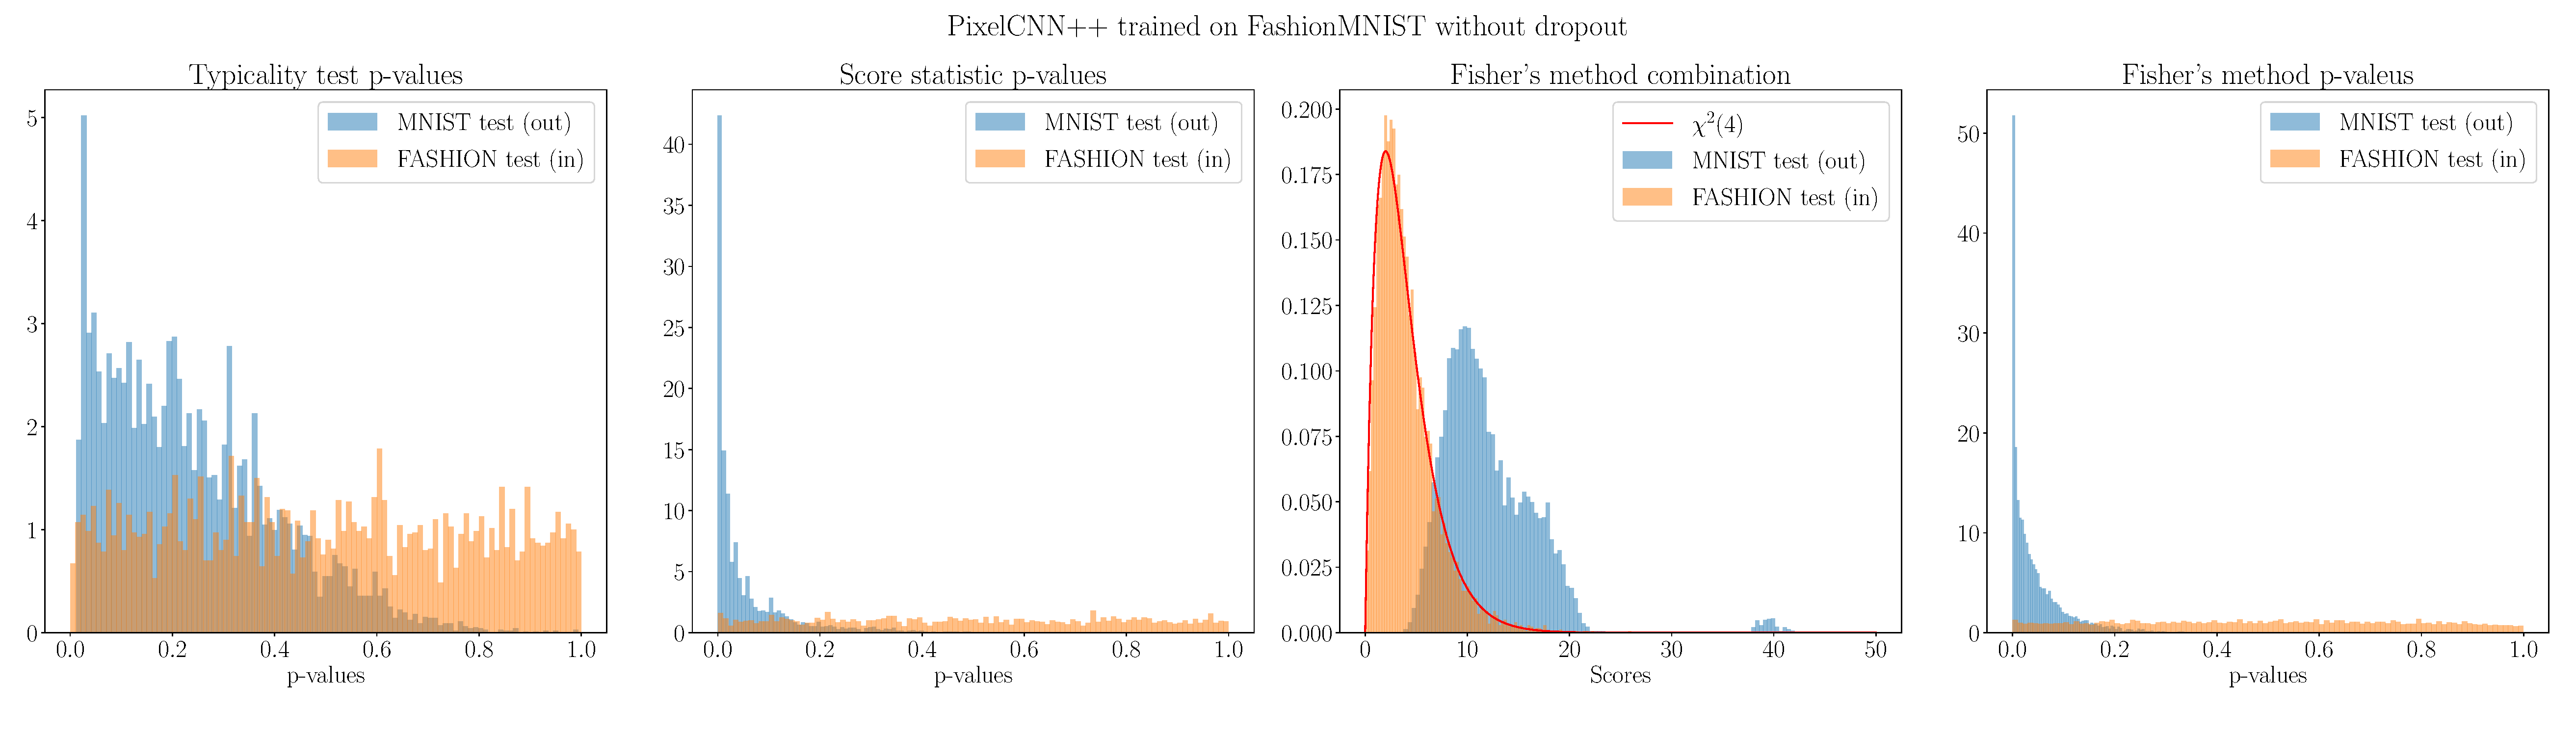
\includegraphics[width=\textwidth]{graphics/paper_modelagnostic/pvalues_comb_no_drop_correct_font.pdf}
    \caption[Distribution of the p-values of the typicality test, score statistic, Fisher's method and a combination of all.]{ \emph{First plot}: $p$-values of the typicality test on the two test sets. We can see that under $\mathcal{H}_0$, they should be uniformly distributed. \emph{Second plot}: $p$-values of the score statistic. \emph{Third plot}: values obtained by the Fisher's method. In red, we plot the density function of a $\chi^2$-distribution with 4 degrees. This shows that the statistics are independent. \emph{Fourth plot}: $p$-values obtained of the combination. These plots refer to a PixelCNN++ trained on FashionMNIST without dropout.}
    \label{fig_modelagnostic:comb_p_values}
\end{sidewaysfigure} 

\begin{table*}[tb]
    %\renewcommand{\thetable}{4}
    \caption{AUROC$\uparrow$ for single-sample OOD detection. For Fisher's method we mean the combination of the typicality test and the test statistic. These are also combined using DoSE.}
    \resizebox{\textwidth}{!}{
        \scriptsize
        \begin{tabular}{ccccccc}
            \toprule
            &\multicolumn{6}{c}{\textsc{FashionMNIST (in) / MNIST (out)}}\\
            \cmidrule{2-7}
            & \multicolumn{4}{c}{\textcolor{blue}{\textsc{single statistics}}} & \multicolumn{2}{c}{\textcolor{red}{\textsc{combination}}}\\
            \cmidrule(r){2-5}\cmidrule(l){6-7}
            \textsc{models}  & \textcolor{blue}{\textsc{$\log p(x)$}} & \textcolor{blue}{\textsc{$\|\nabla \log p(x)\|_2$}} & \textcolor{blue}{\textsc{Typicality}} & \textcolor{blue}{\textsc{Score Stat}} & \textcolor{red}{\textsc{Fisher's method}} & \textcolor{red}{\textsc{DoSE$_{\textup{KDE}}$}} \\
            \midrule
            \textsc{PixelCNN++} (dropout)  &  0.0762 & 0.8709 & 0.8314 & \textbf{0.8822} & \textbf{0.9369}  & 0.8822 \\
            \textsc{PixelCNN++} (no dropout)  & 0.1048 &  \textbf{0.9532} &  0.7575 &  0.9381 & \textbf{0.9536} &  0.9382 \\
            \textsc{Glow} (RMSProp) &  0.1970 & 0.8904  & 0.4807 &  \textbf{0.9114} & 0.8598  &  \textbf{0.8901}\\
            \textsc{Glow} (Adam)  & 0.1223 & 0.7705 & 0.6987 &  \textbf{0.8745} & \textbf{0.8839}  & 0.8752 \\
            \textsc{HVAE}  & 0.2620 & 0.8714 &0.4884 & \textbf{0.9578} & 0.9383 & \textbf{0.9498} \\
            \bottomrule
            & & & & & & \\
            \toprule
            &\multicolumn{6}{c}{\textsc{CIFAR10 (in) / SVHN (out)}}\\
            \cmidrule{2-7}
            & \multicolumn{4}{c}{\textcolor{blue}{\textsc{single statistics}}} & \multicolumn{2}{c}{\textcolor{red}{\textsc{combination}}}\\
            \cmidrule(r){2-5}\cmidrule(l){6-7}
            \textsc{models}  & \textcolor{blue}{\textsc{$\log p(x)$}} & \textcolor{blue}{\textsc{$\|\nabla \log p(x)\|_2$}} & \textcolor{blue}{\textsc{Typicality}} & \textcolor{blue}{\textsc{Score Stat}} & \textcolor{red}{\textsc{Fisher's method}} & \textcolor{red}{\textsc{DoSE$_{\textup{KDE}}$}} \\
            \midrule
            \textsc{PixelCNN++} (model1)  & 0.1553 & \textbf{0.8006} &  0.6457 & 0.6407 & \textbf{0.6826} & 0.6571 \\
            \textsc{PixelCNN++} (model2) & 0.1567 & \textbf{0.7923} & 0.6498 &  0.7067 & \textbf{0.7300} & 0.7243 \\
            \textsc{Glow} (RMSProp)  &  0.0630 & 0.8585 & \textbf{0.8651} &  0.7940 &  \textbf{0.8683} & 0.8510 \\
            \textsc{Glow} (Adam)   &  0.0627 & 0.7844 &  \textbf{0.8624} &  0.7655 &  \textbf{0.8613} &  0.8588 \\
            \textsc{HVAE}  & 0.0636 & 0.8067  & \textbf{0.8679} & 0.7335 & \textbf{0.8603} & 0.8179 \\
            \bottomrule
            & & & & & & \\
            \toprule
            &\multicolumn{6}{c}{\textsc{CIFAR10 (in) / CIFAR100 (out)}}\\
            \cmidrule{2-7}
            & \multicolumn{4}{c}{\textcolor{blue}{\textsc{single statistics}}} & \multicolumn{2}{c}{\textcolor{red}{\textsc{combination}}}\\
            \cmidrule(r){2-5}\cmidrule(l){6-7}
            \textsc{models}  & \textcolor{blue}{\textsc{$\log p(x)$}} & \textcolor{blue}{\textsc{$\|\nabla \log p(x)\|_2$}} & \textcolor{blue}{\textsc{Typicality}} & \textcolor{blue}{\textsc{Score Stat}} & \textcolor{red}{\textsc{Fisher's method}} & \textcolor{red}{\textsc{DoSE$_{\textup{KDE}}$}} \\
            \midrule
            \textsc{PixelCNN++} (model1)  & 0.5153 & 0.5306 & \textbf{0.5458} & 0.5362 & \textbf{0.5563}  & 0.5477\\
            \textsc{PixelCNN++} (model2) & 0.5150 &  0.5230 & \textbf{0.5455} & 0.5325  & \textbf{0.5543} & 0.5453 \\
            \textsc{Glow} (RMSProp)  &  0.5206 & 0.5547 & 0.5507 & 0.\textbf{5801} & \textbf{0.5844} &  \textbf{0.5842} \\
            \textsc{Glow} (Adam)   & 0.5206 & 0.5593 & 0.5508  & \textbf{0.5692} & \textbf{0.5775} &  \textbf{0.5767} \\
            \textsc{HVAE}  & 0.5340 & 0.5280 &  0.5493 &  \textbf{0.5798} &  0.5879 &  \textbf{0.5941}\\
            \bottomrule 
        \end{tabular}
        \label{tab_modelagnostic:single_sample_results}
    }
    \vspace*{-\baselineskip}
\end{table*}





%% %%%%%%%%%%%%%%%%%%%%%%%%%%%%%%%%%%  SECTION 5: EXP SETUP   %%%%%%%%%%%%%%%%%%%%%%%%%%%%%%%%%%
\section{Experimental Setup}

To evaluate the performance of the combination of the typicality test and the score statistic in detecting OOD data, we follow the experiments of \textcite{nalisnick_deep_2019, hendrycks_deep_2019} and considered the OOD detection task on three image dataset pairs that have been proven challenging for DGMs, i.e.\@ FashionMNIST \parencite{xiao_fashionmnist_2017} vs MNIST \parencite{lecun_mnist_1998}, CIFAR10 \parencite{krizhevsky_learning_2009} vs SVHN \parencite{netzer_reading_2011}, and CIFAR10 vs CIFAR100. \textcite{winkens_contrastive_2020} divide these tasks into \textit{far}-OOD tasks, where the in-distribution and out-distribution are different such as in the case of CIFAR10 against SVHN, and \textit{near}-OOD where the two distributions are pretty similar, such as CIFAR10 and CIFAR100. \textit{Near}-OOD tasks are usually most challenging.

For each task, we trained three different state-of-the-art DGMs, a PixelCNN++ \parencite{salimans_pixelcnn_2017}, a Glow model \parencite{kingma_glow_2018}, and a hierarchical variational autoencoder \parencite{kingma_autoencoding_2014,rezende_stochastic_2014} with bottom-up inference (HVAE, \citealp{burda_importance_2016}). These are DGMs parametrized by neural networks that make different assumptions in the modelling choice of the target distribution. In addition to that, for PixelCNN++ and Glow we have a tractable likelihood while for HVAE we can only estimate a lower bound. A more in-depth description of these methods and additional results testing MNIST against FashionMNIST and SVHN against CIFAR10 can be found in \cref{appendix_modelagnostic:mnist_svhn}. We also extensively analyzed, focusing mostly in the influence of the preprocessing, the results on CIFAR10 vs CelebA \parencite{liu_deep_2015} in \cref{appendix_modelagnostic:celeba}. In \cref{appendix_modelagnostic:gmm_ppca}, we also considered a Gaussian Mixture Model and a Probabilistic PCA as simple generative models.

\paragraph{Models} To analyze the effect of model architecture choices and optimization choice, we also consider different versions of the same model that reaches a similar log-likelihood. We consider 5 different models for each dataset pair. On FashionMNIST, we consider two Glow models, one trained using Adam and one using RMSProp and two PixelCNN++, trained with and without dropout. For CIFAR10, we consider two different PixelCNN++, one trained by us (model1) and one using a checkpoint given by the repository we used\footnote{ \href{https://github.com/pclucas14/pixel-cnn-pp}{\texttt{https://github.com/pclucas14/pixel-cnn-pp}}} (model2), and two Glow models (Adam and RMSProp). For both datasets, instead, we consider only one HVAE. 


\paragraph{Baselines} We are mostly interested in testing our methods with other model-agnostic test statistics in the literature. Apart from using the plain likelihood as an OOD score, the only test statistic we are aware of that can be applied to any generative model without requiring any background model or OOD assumptions is the typicality test statistic of \textcite{nalisnick_detecting_2019}. We also considered the gradient norm, which in general seem to work well but fails in the case of SVHN vs CIFAR10 (see \cref{appendix_modelagnostic:mnist_svhn}). In addition to that, we compare our methods to a model-agnostic version of DoSE by \textcite{morningstar_density_2021}, where we used KDEs to combine the score statistic and the typicality test statistic. 


\paragraph{Evaluation} We compare our methods with the baselines by computing the area under the receiver operating characteristic curve (AUROC) as done in previous works \parencite{hendrycks_deep_2019, ren_likelihood_2019, morningstar_density_2021}. We also evaluate our methods in terms of False Discovery Rate (FDR) control \textcite{benjamini_controlling_1995}, i.e.\@ the proportion of false positive among the rejected hypothesis. Note that both quantities need to know the true label (OOD or in-distribution) to be computed.


%% %%%%%%%%%%%%%%%%%%%%%%%%%%%%%%%%%%  SECTION 5: RESULTS   %%%%%%%%%%%%%%%%%%%%%%%%%%%%%%%%%%
\section{Results}

\paragraph{One-sample OOD}
We first evaluate our proposed method in the single-sample OOD detection task. Results are summarized in \cref{tab_modelagnostic:single_sample_results}. We start by considering the OOD task on FashionMNIST against MNIST. Looking at the single statistics, we notice that the score statistic is the one that works the best and the combination of the typicality test and the score statistic usually improve the AUROC than the two standalone statistics. In addition to that, it is better than the combination of the two statistics by using a KDE. DoSE seems to perform better on Glow trained with RMSProp, where the typicality is failing. 

On natural images, instead, we have a different trend. The typicality test is better than the score statistic overall. The gradient norm surprisingly performs well in the two dataset pairs, but it fails badly when the model is trained on SVHN (see \cref{appendix_modelagnostic:mnist_svhn}). Regarding the combination of the two statistics, the Fisher's method is always better than DoSE, but in this setting, it improves over the best of the single statistics three out of five times.
%
In the \textit{near}-OOD task, we have that both our method and DoSE using our suggested statistics perform closely. We want to highlight that for this challenging task we get results that are comparable with those reported in \textcite{morningstar_density_2021}, but by using two model-agnostic statistics instead of three model-specific ones.
%
It can be noticed that the way we train our models has a strong influence on both the typicality test and the score statistic, although the models get the same test log-likelihood. In \cref{appendix_modelagnostic:checkpoints}, we also show that this can happen between different checkpoints of the same model.

In \cref{fig_modelagnostic:comb_p_values}, we show that the $p$-values distributions for both the typicality and the score statistic are uniformly distributed under the null-hypothesis and that the combination under the null follows a $\chi^2$ distribution with 4 degrees of freedom. This also supports the fact that the typicality test and the score statistic are independent.

\paragraph{Two-sample OOD}
As \textcite{nalisnick_detecting_2019}, we consider how these test statistics change when performing two-sample OOD detection. Results are summarized in \cref{tab_modelagnostic:two_sample_results}. As shown by \textcite{nalisnick_detecting_2019}, the typicality improves, but also the score statistic gets better if we consider more samples. Combining those leads to an improvement of performance in terms of AUROC with almost all the models. When training on FashionMNIST, the model can almost perfectly distinguish between the in-distribution test set and the OOD test set. While the performance improves for the two \textit{far}-OOD task, we have that the improvement is slightly less evident in the \textit{near}-OOD task of CIFAR10 vs CIFAR100.

\begin{table}[t]
\scriptsize
\centering
\caption{AUROC$\uparrow$ for two-sample OOD detection using the usual considered model.}\normalsize
    %\renewcommand{\thetable}{4}
    \resizebox{0.90\textwidth}{!}{
        \scriptsize
        \begin{tabular}{ccccc}
            \toprule
            &\multicolumn{4}{c}{\textsc{FashionMNIST (in) / MNIST (out)}}\\
            \cmidrule{2-5}
            \textsc{models}  & \textcolor{blue}{\textsc{Typicality}} & \textcolor{blue}{\textsc{Score Stat}} & \textcolor{red}{\textsc{Fisher's method}} & \textcolor{red}{\textsc{DoSE$_{\textup{KDE}}$}} \\
            \midrule
            \textsc{PCNN++} (drop.) &  0.9514 & 0.9828 & \textbf{0.9934} & \textbf{0.9912} \\
            \textsc{PCNN++} (no drop)  & 0.9081 &   0.9853 & \textbf{0.9916} &  \textbf{0.9921} \\
            \textsc{Glow} (RMSProp) & 0.6190 &  \textbf{0.9588} &  0.9187 & 0.7201  \\
            \textsc{Glow} (Adam)  & 0.8525 &  \textbf{0.9716} & \textbf{0.9708} & \textbf{0.9736} \\
            \textsc{HVAE}  & 0.6634 & \textbf{0.9881} & \textbf{0.9837} &  \textbf{0.9889}\\
            \bottomrule
            & & & &\\
            \toprule
            &\multicolumn{4}{c}{\textsc{CIFAR10 (in) / SVHN (out)}}\\
            \cmidrule{2-5}
            \textsc{models}  & \textcolor{blue}{\textsc{Typicality}} & \textcolor{blue}{\textsc{Score Stat}} & \textcolor{red}{\textsc{Fisher's method}} & \textcolor{red}{\textsc{DoSE$_{\textup{KDE}}$}} \\
            \midrule
            \textsc{PCNN++} (m1) & 0.7675 & 0.6555 & \textbf{0.7800} &  0.7046\\
            \textsc{PCNN++} (m2) & 0.7720 &   0.7235 & \textbf{0.8227} & 0.7850\\
            \textsc{Glow} (RMSProp)  & 0.9497 &  0.8624 & \textbf{0.9536} & 0.9379\\
            \textsc{Glow} (Adam) & 0.9480 &  0.8370 & \textbf{0.9519} & 0.9329\\
            \textsc{HVAE} &  \textbf{0.9623} &  0.7754 &  0.9560 & 0.9133\\
            \bottomrule
            & & & &\\
            \toprule
            &\multicolumn{4}{c}{\textsc{CIFAR10 (in) / CIFAR100 (out)}}\\
            \cmidrule{2-5}
            \textsc{models}  & \textcolor{blue}{\textsc{Typicality}} & \textcolor{blue}{\textsc{Score Stat}} & \textcolor{red}{\textsc{Fisher's method}} & \textcolor{red}{\textsc{DoSE$_{\textup{KDE}}$}} \\
            \midrule
            \textsc{PCNN++} (m1) &  0.5433 & 0.5450 &  \textbf{0.5540} &  \textbf{0.5508}\\
            \textsc{PCNN++} (m2) &  0.5435 &  0.5370 &  \textbf{0.5533} & 0.5470 \\
            \textsc{Glow} (RMSProp)  & 0.5550 &  \textbf{0.6211}  & 0.6165 &  \textbf{0.6233}\\
            \textsc{Glow} (Adam) & 0.5558  &   0.6073 & 0.6083 &   \textbf{0.6117}\\
            \textsc{HVAE} & 0.5594  & 0.6188  &  \textbf{0.6218} & \textbf{0.6273} \\
            \bottomrule
        \end{tabular}
        \label{tab_modelagnostic:two_sample_results}
    }
    \vspace*{-\baselineskip}
\end{table}


\subsection{Practical OOD detection with FDR control}
One of the advantages of framing the problem as multiple testing is that we have a well-defined procedure to decide on which hypotheses to reject while controlling the False Discovery Rate (FDR, \citealp{benjamini_controlling_1995}). Imagine we are interested in finding the outliers from the dataset given by the combination of the two test-sets, but we do not want to discard too many inliers, then we can use the Benjamini-Hochberg (BH) procedure \parencite{benjamini_controlling_1995} to decide a threshold and reject all hypothesis below that threshold. For a specific significance level $\alpha$, the procedure guarantees that the FDR stays below that level. Therefore, we can guarantee that the rate of inliers that are classified as outliers is less than the chosen $\alpha$.

%As we have mentioned before, when combining $p$-values of $k$ different statistics using the Fisher's method if the null hypothesis is true, then these new scores are $\chi^2_{2k}$. This allows us to easily compute the $p$-values associate to those new values and then apply the Benjamini-Hochberg procedure. Alternatively, one can directly apply the procedure to the $p$-values of a single test-statistic.

We leverage the fact that when the null hypothesis is true and the $p$-values are independent, then the scores obtained by combining $k$ different statistics are $\chi^2_{2k}$ distributed to compute the $p$-values. Alternatively, the procedure can be also applied to the $p$-values of a single test-statistic.
%
Usually, it is better to use an FDR control when it is actually possible to make few false discoveries, i.e.\@ when we have a strong statistic. Therefore, we expect the procedure to work well when the AUROC is good, for examples on models trained on FashionMNIST.

As can be seen in \cref{fig_modelagnostic:type1}, we have that the Type I ratio line stays below the identity line, meaning that the BH correction is working. When deciding for a specific threshold $\alpha$, we usually have to trade off between Type I and Type II error and in most cases the threshold to choose depends on the application domain. Ideally, we would like to have a low Type I and a low Type II error rate, meaning that we are not considering a lot of in-distribution examples as OOD and at the same time considering a lot of outliers as in-distribution. \cref{fig_modelagnostic:type1} shows that we can achieve this for low values of $\alpha$. When training on CIFAR, instead, we are able to control the FDR only from a certain significance level (see \cref{appendix_modelagnostic:BH_cifar}). This is expected given that the AUROC is not as good as when testing on MNIST.


%%%%%%%%%%%%%%%%%%%%%%% FIGURE
\begin{figure}[tb]
    \centering
    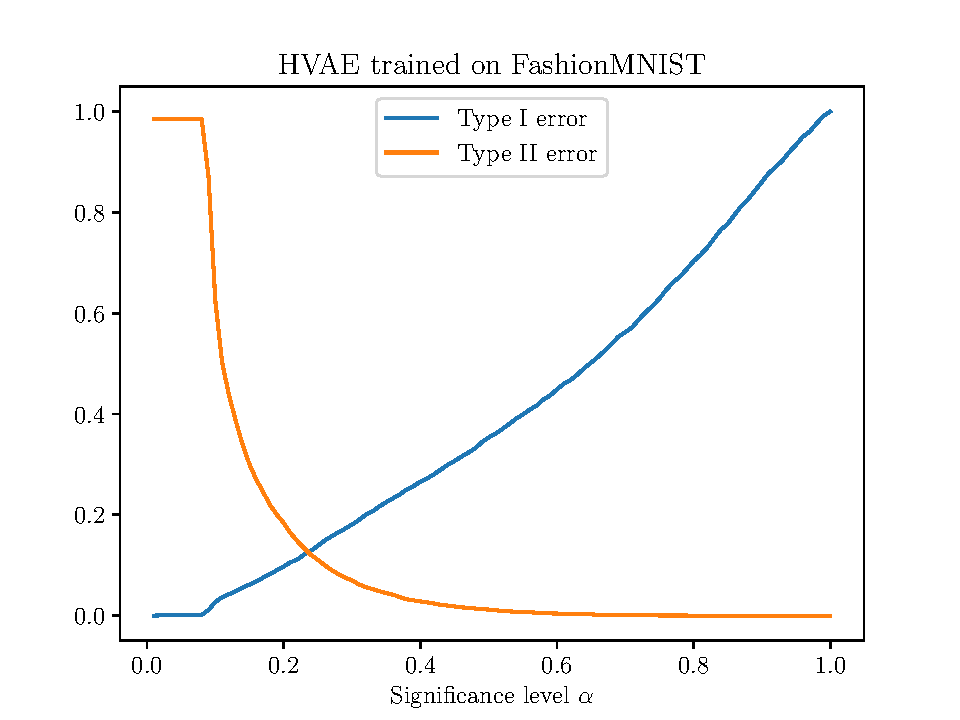
\includegraphics[scale=0.6]{graphics/paper_modelagnostic/fashion_hvae_type1_correct_font.pdf}
    \caption[Type I and Type II errors versus the significance level $\alpha$ on the combination values.]{ Type I (probability of an inlier to be classified as outlier) and Type II (probability of an outlier to be considered as inlier) errors versus the significance level $\alpha$ on the combination values. By using Benjamini-Hochberg correction, we get that the Type I error stays below identity line.}
    \label{fig_modelagnostic:type1}
\end{figure}


%% %%%%%%%%%%%%%%%%%%%%%%%%%%%%%%%%%%  SECTION 5: CONCLUSION   %%%%%%%%%%%%%%%%%%%%%%%%%%%%%%%%%%
\section{Discussion and Conclusions}
In this paper we studied the task of out-of-distribution detection using deep generative models and a combination of multiple statistical tests. We tested our method using different state-of-the art DGMs on classic image benchmark for OOD detection. We found that combining the two statistic leads to a more robust score that in some cases is close to state-of-the-art model-specific scores that require more assumptions. We also noticed that both the model design choice and the optimization choices have an influence on the score we are computing. 

When considering only one-sided independent statistics, we showed that the Fisher's method tends to work better than combine them by summing the log-density of a KDE. We also noticed that the score statistic tends to perform a bit worse when the number of parameters of the models increases, i.e.\@ in the context of natural images. One possible reason can be that in this setting the diagonal approximation is not good, and therefore one could consider different approximations, such as K-FAC. 

DGMs have recently been used for handling missing data (see e.g.\@ \citealp{mattei_miwae_2019, ma_eddi_2019, nazabal_handling_2020, ipsen_not-miwae_2021}). An interesting future direction would be to extend these OOD detection methods to handle missing values.

The methods  presented in this paper can also easily be applied when using model-specific one-sided statistics. In addition to obtain a more accurate score if one want to combine the test statistics, this also allows one to use well-defined procedure to control the FDR when choosing a which example to mark as outliers. Having this control, is necessary when we want to apply these methods in real settings. 


\section*{Acknowledgements}
Federico Bergamin and Pierre-Alexandre Mattei contributed equally to this paper, which is indicated by the asterisk (*) in the author list. The work was supported by the Innovation Fund Denmark (0175-00014B and 0153-00167B), the Independent Research Fund Denmark (9131-00082B) and the Novo Nordisk Foundation (NNF20OC0062606 and NNF20OC0065611). Furthermore, it was supported by the French government, through the 3IA Côte d'Azur Investments in the Future project managed by the National Research Agency (ANR) with the reference number ANR-19-P3IA-0002.


}
%!TEX root = ../thesis.tex

\chapter[benchmarking generative latent variable models for speech]{Benchmarking Generative Latent Variable Models for Speech}
\label{chp:paper-benchmarking}

\textit{This chapter is a piece of original research published as part of the project:} \newline
\begin{center}
    \begin{enumerate}[leftmargin=8mm,rightmargin=8mm,topsep=0mm,label={[\Alph*]}]
        \setcounter{enumi}{3}
        \item \fullcite{havtorn_benchmarking_2022} \main \. \parencite{havtorn_benchmarking_2022}
        \end{enumerate}
\end{center}

\ifthenelse{\equal{\skippapers}{true}}{}{


\section{Abstract}
Stochastic latent variable models (LVMs) achieve state-of-the-art performance on natural image generation but are still inferior to deterministic models on speech. In this paper, we develop a speech benchmark of popular temporal LVMs and compare them against state-of-the-art deterministic models. We report the likelihood, which is a much used metric in the image domain, but rarely, or incomparably, reported for speech models. To assess the quality of the learned representations, we also compare their usefulness for phoneme recognition. Finally, we adapt the Clockwork VAE, a state-of-the-art temporal LVM for video generation, to the speech domain. Despite being autoregressive only in latent space, we find that the Clockwork VAE can outperform previous LVMs and reduce the gap to deterministic models by using a hierarchy of latent variables.


\section{Introduction}
After the introduction of the variational autoencoder (VAE,  \textcite{kingma_autoencoding_2014, rezende_stochastic_2014}) quickly came two temporal extensions for modeling speech data \parencite{chung_recurrent_2015, fraccaro_sequential_2016}. Since then, temporal LVMs have undergone little development compared to their counterparts in the image domain, where LVMs recently showed superior performance to autoregressive models such as PixelCNN \parencite{oord_pixel_2016, oord_conditional_2016, salimans_pixelcnn_2017}. The improvements in the image domain have been driven mainly by top-down inference models and deeper latent hierarchies \parencite{sonderby_ladder_2016, maaloe_biva_2019, vahdat_nvae_2020, child_very_2021,sinha_consistency_2021,kingma_variational_2021}. In speech modeling however, autoregressive models such as the WaveNet remain state-of-the-art \parencite{oord_wavenet_2016}.

To compare and develop LVMs for speech, we need good benchmarks similar to those in the image domain. Image benchmarks commonly compare likelihood scores, but research in the speech domain often omits reporting a likelihood \parencite{oord_wavenet_2016, hsu_unsupervised_2017, oord_neural_2018} or report likelihoods that are incomparable due to subtle differences in the assumed data distribution \parencite{chung_recurrent_2015, fraccaro_sequential_2016, hsu_unsupervised_2017, aksan_stcn_2019}. Without a proper standard, it is difficult to compare explicit likelihood models for speech and develop them in an informed manner.

To advance the state of LVMs for speech, this paper (i) develops a benchmark for LVMs based on model likelihood, (ii) introduces a hierarchical LVM architecture without autoregressive decoder, (iii) compares LVMs to deterministic counterparts including WaveNet, and (iv) qualitatively and quantitatively evaluates the latent variables learned by different LVMs based on their usefulness for phoneme recognition. We find that:
\begin{itemize}[leftmargin=8mm]
    \setlength\itemsep{-0em}
    \item [(I)] State-of-the-art LVMs achieve likelihoods that are inferior to WaveNet at high temporal resolution but are superior at lower resolutions. Interestingly, we find that a standard LSTM \parencite{hochreiter_long_1997} almost matches the likelihood of WaveNet.
    \item [(II)] LVMs with powerful autoregressive decoders achieve better likelihoods than the non"=autoregressive LVM.
    \item[(III)] The expressiveness of LVMs for speech increases with a deeper hierarchy of stochastic latent variables, similar to conclusions within image modeling. % \parencite{maaloe_biva_2019, vahdat_nvae_2020, child_very_2021}.
    \item[(IV)] LVMs learn rich representations that are as good or better than Mel spectrograms for phoneme recognition also when using only 10 minutes of labeled data.
\end{itemize}
At a high level, this benchmark brings order to LVM model comparisons for speech and also provides useful reference implementations of the models\footnote{\href{https://github.com/JakobHavtorn/benchmarking-lvms}{\url{github.com/JakobHavtorn/benchmarking-lvms}}}.
% \footnote{\fontsize{8.5}{0}\selectfont\texttt{ \url{github.com/anonymous/available-later}}}.
Before presenting the results, we provide a brief survey of existing LVMs for speech in a coherent notation. 


\section{Latent variable models for speech}
\begin{figure*}[t]
    \centering
    \begin{multicols}{5}
        \resizebox{!}{0.18\paperheight}{
            \begin{tikzpicture}
                \node[obs] (x_t) {$\xb_t$};
                
                % \node[above=0.75cm of x_t, xshift=0cm] (cap1) {$p(\xb_t|\xb_{<t})$};
                \node[above=0.4cm of x_t] (caption) {LSTM};
                
                \node[det,below=2.55cm of x_t] (d_t) {$\db_{t}$};
                \node[det,left=0.75cm of d_t] (d_tm1) {$\db_{t-1}$};
                \node[obs,below=0.75cm of d_t] (x_tm1) {$\xb_{t-1}$};
                
                \edge[deterministic-skip-color]{x_tm1}{d_t};
                \edge[deterministic-skip-color]{d_t}{x_t};
                \edge[deterministic-skip-color]{d_tm1}{d_t};
                \edge[draw=white,bend right]{d_t}{x_t};  % for identical width to others
            \end{tikzpicture}
        }
        \\
        \resizebox{!}{0.18\paperheight}{
            \begin{tikzpicture}
                \node[obs] (x_t) {$\xb_t$};
                
                % \node[above=0.75cm of x_t, xshift=0cm] (cap1) {$p(\xb_t|\zb_{\leq t},\xb_{<t}) p(\zb_t|\xb_{<t},\zb_{<t})$};
                \node[above=0.4cm of x_t] (caption) {VRNN};
                
                \node[latent,below=0.75cm of x_t] (z_t) {$\zb_t$};
                \node[latent,left=0.75cm of z_t] (z_tm1) {$\zb_{t-1}$};
                
                \node[det,below=0.75cm of z_t] (d_t) {$ b_{t}$};
                \node[det,below=0.75cm of z_tm1] (d_tm1) {$\db_{t-1}$};
                \node[obs,below=0.75cm of d_t] (x_tm1) {$\xb_{t-1}$};
                
                \edge[deterministic-skip-color]{x_tm1}{d_t};
                \edge[]{d_t}{z_t};
                \edge[]{z_tm1}{d_t};
                \edge[deterministic-skip-color]{d_tm1}{d_t};
                \edge[]{z_t}{x_t};
                \edge[deterministic-skip-color,bend right]{d_t}{x_t};
            \end{tikzpicture}
        }
        \\
        \resizebox{!}{0.18\paperheight}{
            \begin{tikzpicture}
                \node[obs] (x_t) {$\xb_t$};
                
                % \node[above=0.75cm of x_t, xshift=0cm] (cap1) {$p(\xb_t|\zb_{\leq t},\xb_{<t}) p(\zb_t|\xb_{<t},\zb_{<t})$};
                \node[above=0.4cm of x_t] (caption) {SRNN};
                
                \node[latent,below=0.75cm of x_t] (z_t) {$\zb_t$};
                \node[latent,left=0.75cm of z_t] (z_tm1) {$\zb_{t-1}$};

                \node[det,below=0.75cm of z_t] (d_t) {$\db_{t}$};
                \node[det,below=0.75cm of z_tm1] (d_tm1) {$\db_{t-1}$};
                \node[obs,below=0.75cm of d_t] (x_tm1) {$\xb_{t-1}$};
                
                \edge[deterministic-skip-color]{x_tm1}{d_t};
                \edge[]{d_t}{z_t};
                \edge[]{z_tm1}{z_t};
                \edge[deterministic-skip-color]{d_tm1}{d_t};
                \edge[]{z_t}{x_t};
                \edge[deterministic-skip-color,bend right]{d_t}{x_t};
            \end{tikzpicture}
        }
        \\
        \resizebox{!}{0.18\paperheight}{
            \begin{tikzpicture}
                \node[obs] (x_t) {$\xb_t$};
                % \node[above=0.75cm of x_t, xshift=0cm] (cap1) {$p(\xb_t|\zb_t,\xb_{t-r:t-1})$};
                \node[above=0.4cm of x_t] (caption) {STCN};
                
                \node[latent,below=0.75cm of x_t] (z_t) {$\zb_t$};
                \node[left=0.025cm of z_t] (dots) {$\cdots$};
                \node[latent,left=0.75cm of z_t] (z_tmr) {$\zb_{t-r'}$};
                
                \node[det,below=0.75cm of z_t] (d_t) {$\db_{t}$};
                \node[obs,below=0.75cm of d_t] (x_tm1) {$\xb_{t-1}$};
                \node[left=0.025cm of x_tm1] (dots) {$\cdots$};
                \node[obs,left=0.75cm of x_tm1] (x_tmr) {$\xb_{t-r}$};
                
                \edge[]{x_tm1}{d_t};
                \edge[]{x_tmr}{d_t};
                \edge[]{d_t}{z_t};
                \edge[]{z_t}{x_t};
                \edge[]{z_tmr}{x_t};
                \edge[draw=white,bend right]{d_t}{x_t};  % for identical width to others 
            \end{tikzpicture}
        }
        \\
        \resizebox{!}{0.18\paperheight}{
            \begin{tikzpicture}
                \node[obs] (x_t) {$\xb_t$};%
                
                % \node[above=0.75cm of x_t, xshift=0cm] (cap1) {$p(\xb_t|\zb_{\leq t}) p(\zb_t|\zb_{<t})$};
                \node[above=0.4cm of x_t] (caption) {CW-VAE};
                
                \node[latent,below=0.75cm of x_t] (z_t) {$\zb_t$};
                \node[latent,left=0.75cm of z_t] (z_tm1) {$\zb_{t-1}$};
                
                \node[det,below=0.75cm of z_t] (d_t) {$\db_{t}$};
                \node[det,below=0.75cm of z_tm1] (d_tm1) {$\db_{t-1}$};
                \node[obs,below=0.75cm of d_t,draw=white,fill=white] (x_tm1) {};
                
                \edge[]{d_t}{z_t};
                \edge[bend right]{d_t}{x_t};
                \edge[]{z_tm1}{d_t};
                \edge[]{d_tm1}{d_t};
                \edge[]{z_t}{x_t};
            \end{tikzpicture}
        }
        \end{multicols}
    \caption[Generative models for an LSTM, the VRNN, SRNN, STCN, and CW-VAE models.]{
        Generative models for a single timestep of a deterministic autoregressive LSTM, the VRNN and SRNN as well as the STCN and CW-VAE both with a single layer of latent variables. 
        Red arrows indicate purely deterministic paths from the output $\xb_t$ to previous input $\xb_{<t}$ without passing a stochastic node. 
        The models differ in their use of latent variables and dependencies especially autoregressive dependencies and skip connections. 
        % In an LSTM, information flows deterministically from previous observed variables to the next. 
        % The VRNN and SRNN use stochastic latent variables but also include deterministic skip connections from previous observed variables. 
        % The STCN is also autoregressive in $\xb$ but does not use deterministic skip connections from $\xb_{t-1}$ to $\xb_t$. 
        % The CW-VAE is not autoregressive on the observed variable which forces information to flow through the latent variables. 
        We provide more elaborate graphical illustrations including inference models in \cref{fig: clockwork vae inference generative models 2 layered} and appendix~\cref{app: additional graphical models}.
        }
    \label{fig: autoregressive vrnn srnn cwvae 1L graphs}
\end{figure*}


% \linepenalty=1000
% \subsection{Related work}
LVMs formulated as VAEs continue to be of interest since they are able to learn an approximation to the posterior distribution of assumed latent variables. The posterior is usually of a reduced dimensionality compared to the input and lies close to a known prior distribution. Approximate posteriors have various applications e.g. semi"=supervised learning \parencite{kingma_semi-supervised_2014} and anomaly detection \parencite{havtorn_hierarchical_2021}.

In recent years, several complementary methods have been proposed to improve the expressiveness of VAEs. These include building more expressive priors via methods such as normalizing flows \parencite{rezende_variational_2015} and building a deeper hierarchy of stochastic latent variables such as the Ladder VAE \parencite{sonderby_ladder_2016}. In this research, we focus on the latter due to the recent breakthroughs in image modeling using VAEs without costly autoregressive dependencies on the observed variable \parencite{maaloe_biva_2019,vahdat_nvae_2020,child_very_2021}.

Several works have applied LVMs to speech. Among the first contributions were the VRNN \parencite{chung_recurrent_2015} and SRNN \parencite{fraccaro_sequential_2016} which can be seen as conditional VAEs per timestep. Other recent LVMs include the FH-VAE \parencite{hsu_unsupervised_2017}, which leverages an additional latent variable to capture global features, and Z-forcing \parencite{goyal_zforcing_2017}, which resembles the SRNN but includes an auxiliary task in the latent space to increase its utilization. The VQ-VAE \parencite{oord_neural_2018} is a hybrid between an LVM and an autoregressive model which uses a quantized latent space to improve the quality of generated samples. The Stochastic WaveNet \parencite{lai_stochastic_2018} and STCN \parencite{aksan_stcn_2019} use WaveNet encoder and decoders and temporally independent latent variables.

In this paper, we focus on the VRNN, SRNN and STCN. We exclude the Stochastic WaveNet as it is similar to STCN and achieves inferior likelihoods \parencite{aksan_stcn_2019}. The FH-VAE, with disjoint latent variables and discriminative objective, Z-forcing, with an auxiliary task, and the VQ-VAE, with a quantized latent space and autoregressive prior fitted after training, all introduce significant changes to the original VAE framework and are also not included here.

All selected models have autoregressive generative models which let future observed variables be generated by conditioning on previously generated values. Inspired by recent progress in the image domain, we therefore formulate and benchmark a novel temporal LVM which does not rely on an autoregressive decoder. We do so by adapting the hierarchical Clockwork Variational Autoencoder \parencite{saxena_clockwork_2021}, originally proposed for video generation, to speech.


\subsection{Sequential deep latent variable models}
The selected models are all sequential deep latent variable models trained with variational inference and the reparameterization trick \parencite{kingma_autoencoding_2014}.
% The VRNN, SRNN, STCN and CW-VAE are all autoencoders trained with variational inference and the reparameterization trick \parencite{kingma_autoencoding_2014}. 
They take as input a variable-length sequence $\xb_{1:T} = \left(\xb_1, \xb_2, \dots, \xb_{T}\right)$ with $\xb_t \in \mathbb{R}^{D_x}$. 
% The VRNN, SRNN, STCN and CW-VAE are all VAEs \parencite{kingma_autoencoding_2014} that take as input a variable-length sequence $\xb_{1:T} = \left(\xb_1, \xb_2, \dots, \xb_{T}\right)$ with $\xb_t \in \mathbb{R}^{D_x}$. 
We let $\xb_{1:T}$ refer to the observed variable or a downsampled version of it. We will sometimes use $\xb$ to refer to the sequence $\xb_{1:T}$ when it is not ambiguous.
% In general, $\xb_{1:T}$ may refer to the original observed variable or a deterministically downsampled representation of the observed variable. We will sometimes use $\xb$ to refer to the full sequence $\xb_{1:T}$ when it is not ambiguous.

First, $\xb_{1:T}$ is encoded to a temporal stochastic latent representation $\zb_{1:T} = \left( \zb_1, \zb_2, \dots, \zb_{T} \right)$ with $\zb_t\in \mathbb{R}^{D_z}$. This representation is then used to reconstruct the original input $\xb_{1:T}$.
The latent variable is assumed to follow some prior distribution $p(\zb_t|\cdot)$ where the dot indicates that it may depend on latent and observed variables at previous timesteps, $\zb_{<t}$ and $\xb_{<t}$ where $\zb_{<t} := \left( \zb_1, \zb_2, \dots, \zb_{t-1} \right)$. 

The models are trained to maximize a likelihood objective. The exact marginal likelihood $\log p_\thetab(\xb)$, where $\thetab$ are parameters of the generative model, is intractable to optimize due to the integration over the latent space. Instead, we introduce the variational approximation $q_\phib(\zb|\xb)$ to the true posterior. Via Jensen's inequality this yields the well-known evidence lower bound (ELBO) on the exact likelihood $\mathcal{L}(\thetab,\phib;\xb)$
which can be jointly optimized with respect to  $\{\thetab, \phib\}$ using stochastic gradient descent methods. We omit the $\thetab$ and $\phib$ subscripts for the remainder of the paper.
\begin{equation}
    \log p_\thetab(\xb) = \log \int p_\thetab(\xb,\zb) \, \mathrm{d}\zb  \geq \mathbb{E}_{q_\phib(\zb|\xb)} \left[ \log \frac{p_\thetab(\xb,\zb)}{q_\phib(\zb|\xb)} \right] =: \mathcal{L}(\thetab,\phib;\xb) \label{eq: elbo} \enspace,
\end{equation}
Graphical illustrations of the models can be seen in \cref{fig: autoregressive vrnn srnn cwvae 1L graphs} with more illustrations in appendix~\cref{app: additional graphical models}.


\subsection{Variational recurrent neural network ({\small VRNN})}
The VRNN \parencite{chung_recurrent_2015} is essentially a VAE per timestep. At timestep $t$, the VAE is conditioned on the hidden state of a recurrent neural network (RNN), $\db_{t}\in\mathbb{R}^{D_d}$, with state transition $\db_{t} = f([\xb_{t-1}, \zb_{t-1}], \db_{t-1})$ where $[\cdot, \cdot]$ denotes concatenation. 
The VRNN uses a Gated Recurrent Unit (GRU, \textcite{cho_properties_2014}) for $f$.
The joint distribution factorizes over time and the latent variables are autoregressive in both the observed and latent space,
\begin{equation}
    p(\xb_{1:T},\zb_{1:T}) = \prod_{t=1}^{T} p(\xb_t|\xb_{<t},\zb_{\leq t}) p(\zb_t|\xb_{<t},\zb_{<t}) \enspace . \label{eq: vrnn joint factorization}
\end{equation}
The approximate posterior similarly factorizes over time,
\begin{equation}
    q(\zb_{1:T}|\xb_{1:T}) = \prod_{t=1}^{T} q(\zb_t|\xb_{\leq t},\zb_{<t}) \enspace . \label{eq: vrnn inference factorization}
\end{equation}
From this, the ELBO for the VRNN is
\begin{equation}
    \mathcal{L}(\xb) = ~ \mathbb{E}_{q(\zb_{1:T}|\xb_{1:T})} \bigg[ \sum_{t} \log p(\xb_t|\xb_{<t},\zb_{\leq t}) - D_\text{KL}\left( q(\zb_t|\xb_{\leq t},\zb_{<t}) \parallel p(\zb_t|\xb_{<t},\zb_{<t}) \right)  \bigg] \label{eq: vrnn elbo} \enspace .
\end{equation}
% \begin{equation}
% \begin{split}
%     \mathcal{L}(\xb) =&~ \mathbb{E}_{q(\zb_{1:T}|\xb_{1:T})} \bigg[ \sum_{t} \log p(\xb_t|\xb_{<t},\zb_{\leq t}) \\ & - \text{KL}\left( q(\zb_t|\xb_{\leq t},\zb_{<t}) \parallel p(\zb_t|\xb_{<t},\zb_{<t}) \right)  \bigg] \enspace .
%     \label{eq: vrnn elbo}
% \end{split}
% \end{equation}
The VRNN uses diagonal covariance Gaussian distributions $\mathcal{N}$ for the prior and posterior distributions. We denote the output distribution of choice by $\mathcal{D}$. 
% \begin{align}
%     q(\zb_t|\xb_{\leq t},\zb_{<t}) &= \mathcal{N}\left(\alphab_{q}(\xb_{t},\db_{t})\right) \label{eq: vrnn parameterization inference} \\
%     p(\zb_t|\xb_{<t},\zb_{<t}) &= \mathcal{N}\left(\alphab_{p}(\db_t)\right) \label{eq: vrnn parameterization prior} \\
%     p(\xb_t|\xb_{<t},\zb_{\leq t}) &= \mathcal{D}\left(\betab(\zb_{t},\db_{t})\right) \enspace . \label{eq: vrnn parameterization observation}
% \end{align}
\begin{gather}
    p(\zb_t|\xb_{<t},\zb_{<t}) = \mathcal{N}\left(\alphab_{p}(\db_t)\right) \enspace , \nonumber \\
    p(\xb_t|\xb_{<t},\zb_{\leq t}) = \mathcal{D}\left(\betab(\zb_{t},\db_{t})\right) \enspace , \label{eq: vrnn parameterization generative} \\
    q(\zb_t|\xb_{\leq t},\zb_{<t}) = \mathcal{N}\left(\alphab_{q}(\xb_{t},\db_{t})\right) \enspace . \nonumber 
    \label{eq: vrnn parameterization inference}
\end{gather}
All sets of distributional parameters, $\alphab_q,\alphab_p$ and $\betab$, are the outputs of densely connected neural networks which we notationally overload as functions in equations~\cref{eq: vrnn parameterization generative} and \cref{eq: vrnn parameterization inference}. It is common to refer to $\alphab_q$ as the inference model or encoder and $\betab$ as the decoder. Together with $\betab$, the structural model $\alphab_p$ forms the generative model.

Since the decoder is dependent on $\db_t$, the transition function $f$ allows the VRNN to learn to ignore parts of or the entire latent variable and establish a purely deterministic transition from $\xb_{t-1}$ to $\db_t$ (\cref{fig: autoregressive vrnn srnn cwvae 1L graphs}). This failure mode is commonly referred to as posterior collapse and is a well-known weakness of VAEs with powerful decoders \parencite{bowman_generating_2016, sonderby_ladder_2016}.


\subsection{Stochastic recurrent neural network ({\small SRNN})}
The SRNN \parencite{fraccaro_sequential_2016} is similar to the VRNN but differs by separating the stochastic latent variables from the deterministic representations (\cref{fig: autoregressive vrnn srnn cwvae 1L graphs}). That is, the GRU state transition is independent of $\zb_{1:T}$ such that $\db_{t} = f(\xb_{t-1}, \db_{t-1})$. With this, the joint $p(\xb_{1:T},\zb_{1:T})$ can be written as for the VRNN in \cref{eq: vrnn joint factorization}. The approximate posterior of $\zb_t$ is conditioned on the full observed sequence,
\begin{align}
    \label{eq: srnn inference factorization}
    q(\zb_{1:T}|\xb_{1:T}) = \prod_{t=1}^{T} q(\zb_t|\xb_{1:T},\zb_{t-1}) \enspace .
\end{align}
This is achieved by introducing a second GRU that runs backwards in time with transition $\ab_t = g([\xb_t,\db_t], \ab_{t+1})$. While $p(\xb_t|\xb_{<t},\zb_{\leq t})$ remains as in \cref{eq: vrnn parameterization generative}, we have
\begin{gather}
        p(\zb_t|\xb_{<t},\zb_{<t}) = \mathcal{N}\left(\alphab_{p}(\zb_{t-1},\db_t)\right) \enspace , \nonumber \\
        q(\zb_t|\xb_{1:T},\zb_{<t}) = \mathcal{N}\left(\alphab_{q}(\zb_{t-1},\ab_{t})\right) \enspace . \label{eq: srnn parameterization}
    % p(\xb_t|\xb_{<t},\zb_{\leq t}) &= \mathcal{D}\left(\vrho(\zb_{t},\db_{t})\right) \enspace . \label{eq: srnn parameterization observation}
\end{gather}
By inferring $\zb_t$ conditioned on the full sequence $\xb_{1:T}$, the SRNN performs smoothing. This has been noted to better approximate the true posterior of $\zb_t$ which can be shown to depend on the full observed sequence \parencite{bayer_mind_2021}. Comparatively, the VRNN performs filtering.


\begin{figure*}
    \centering
    % \h3ill
    \resizebox{!}{0.155\paperheight}{
        \begin{tikzpicture}
            % nodes
            \node[obs] (x_1) {$\xb_{t-3}$};
            \node[obs,right=.75cm of x_1] (x_2) {$\xb_{t-2}$};
            \node[obs,right=.75cm of x_2] (x_3) {$\xb_{t-1}$};
            \node[obs,right=.75cm of x_3] (x_4) {$\xb_{t}$};
            \node[obs,right=.75cm of x_4,fill=white,draw=white] (x_5) {$\dots$};

            \node[latent,above=.75cm of x_1](s_1_1){$\zb^{(1)}_{t-3}$};
            \node[latent,above=.75cm of x_2](s_1_2){$\zb^{(1)}_{t-2}$};
            \node[latent,above=.75cm of x_3](s_1_3){$\zb^{(1)}_{t-1}$};
            \node[latent,above=.75cm of x_4](s_1_4){$\zb^{(1)}_{t}$};
            \node[latent,above=.75cm of x_5,fill=white,draw=white](s_1_5){$\dots$};

            \node[latent,above=.75cm of s_1_1](s_2_1){$\zb^{(2)}_{t-3}$};
            \node[latent,above=.75cm of s_1_3](s_2_3){$\zb^{(2)}_{t-1}$};
            \node[latent,above=.75cm of s_1_5,fill=white,draw=white](s_2_5){$\dots$};

            % x to s first layer
            \edge[]{x_1}{s_1_1};
            \edge[]{x_2}{s_1_2};
            \edge[]{x_3}{s_1_3};
            \edge[]{x_4}{s_1_4};

            % x to s above layer
            \edge[bend left=40]{x_1}{s_2_1};
            \edge[]{x_2}{s_2_1};
            \edge[bend left=40]{x_3}{s_2_3};
            \edge[]{x_4}{s_2_3};

            % s per layer forward in time
            \edge[shared-function-color]{s_1_1}{s_1_2};
            \edge[shared-function-color]{s_1_2}{s_1_3};
            \edge[shared-function-color]{s_1_3}{s_1_4};
            \edge[shared-function-color]{s_1_4}{s_1_5};
            
            \edge[shared-function-color]{s_2_1}{s_2_3};
            \edge[shared-function-color]{s_2_3}{s_2_5};
            
            % s across layers on time
            \edge[shared-function-color]{s_2_1}{s_1_1};
            \edge[shared-function-color]{s_2_3}{s_1_3};

            % s across layers forward in time
            \edge[shared-function-color]{s_2_1}{s_1_2};
            \edge[shared-function-color]{s_2_3}{s_1_4};
            
            % \node[above=of s_2_1, yshift=-1.cm, xshift=2cm] (phi) {$q\pa{\zb_{1:T}^{(1:L)}|\xb_{1:T}}$};
            \node[above=of s_2_1, yshift=-0.5cm, xshift=2.5cm] (phi) {CW-VAE inference};
        \end{tikzpicture}
    }
    \hfill
    \resizebox{!}{0.155\paperheight}{
        \begin{tikzpicture}
            % nodes
            \node[obs] (x_1) {$\xb_{t-3}$};
            \node[obs,right=.75cm of x_1] (x_2) {$\xb_{t-2}$};
            \node[obs,right=.75cm of x_2] (x_3) {$\xb_{t-1}$};
            \node[obs,right=.75cm of x_3] (x_4) {$\xb_{t}$};
            \node[obs,right=.75cm of x_4,fill=white,draw=white] (x_5) {$\dots$};

            \node[latent,above=.75cm of x_1](s_1_1){$\zb^{(1)}_{t-3}$};
            \node[latent,above=.75cm of x_2](s_1_2){$\zb^{(1)}_{t-2}$};
            \node[latent,above=.75cm of x_3](s_1_3){$\zb^{(1)}_{t-1}$};
            \node[latent,above=.75cm of x_4](s_1_4){$\zb^{(1)}_{t}$};
            \node[latent,above=.75cm of x_5,fill=white,draw=white](s_1_5){$\dots$};

            \node[latent,above=.75cm of s_1_1](s_2_1){$\zb^{(2)}_{t-3}$};
            \node[latent,above=.75cm of s_1_3](s_2_3){$\zb^{(2)}_{t-1}$};
            \node[latent,above=.75cm of s_1_5,fill=white,draw=white](s_2_5){$\dots$};

            % x to s first layer
            \edge[]{s_1_1}{x_1};
            \edge[]{s_1_2}{x_2};
            \edge[]{s_1_3}{x_3};
            \edge[]{s_1_4}{x_4};

            % s per layer forward in time
            \edge[shared-function-color]{s_1_1}{s_1_2};
            \edge[shared-function-color]{s_1_2}{s_1_3};
            \edge[shared-function-color]{s_1_3}{s_1_4};
            \edge[shared-function-color]{s_1_4}{s_1_5};
            
            \edge[shared-function-color]{s_2_1}{s_2_3};
            \edge[shared-function-color]{s_2_3}{s_2_5};
            
            % s across layers on time
            \edge[shared-function-color]{s_2_1}{s_1_1};
            \edge[shared-function-color]{s_2_3}{s_1_3};
            
            % s across layers forward in time
            \edge[shared-function-color]{s_2_1}{s_1_2};
            \edge[shared-function-color]{s_2_3}{s_1_4};

            % \node[above=of s_2_1, yshift=-1.cm, xshift=2cm] (phi) {$p\pa{\xb_{1:T},\zb_{1:T}^{(1:L)}}$};
            \node[above=of s_2_1, yshift=-0.5cm, xshift=2.5cm] (phi) {CW-VAE generative};
        \end{tikzpicture}
    % \hfill
    }
\caption[Generative and inference models for a two-layered CW-VAE.]{
Inference (left) and generative (right) models for the CW-VAE with a hierarchy of $L=2$ latent variables, $s_1=1$ and $s_2=2$. 
The models are unrolled over four consecutive timesteps but note that the graph continues towards $t=0$ and $t=T$. 
Blue arrows indicate parameter sharing between inference and generative models. 
We omit the deterministic variable of \cref{fig: autoregressive vrnn srnn cwvae 1L graphs} for clarity.
}
\label{fig: clockwork vae inference generative models 2 layered}
\end{figure*}


\subsection{Stochastic temporal convolutional network ({\small STCN})}
The STCN \parencite{aksan_stcn_2019} is a hierarchical latent variable model with an autoregressive generative model based on WaveNet \parencite{oord_wavenet_2016}. Contrary to VRNN and SRNN, the latent variables have no transition functions connecting them over time.
Instead, a latent $\zb_t^{(l)}$ at layer $l$ is conditioned on a window of observed variables $\xb_{\scriptscriptstyle\mathcal{R}_t^{(l)}}$ via a WaveNet encoder where $\mathcal{R}_t^{(l)} = \cbra{t-r_l+1,\dots,t}$ and $r_l$ is the receptive field of the encoder at layer $l$. The window size grows exponentially with $l$.
\begin{equation}
    p(\xb_{1:T},\zb_{1:T}^{(1:L)}) = \prod_{t=1}^{T} p(\xb_t|\zb^{(1:L)}_{{\scriptscriptstyle \mathcal{R}}_{t}^{(1)}}) \prod_{l=1}^{L} p(\zb^{(l)}_{t}|\xb_{\scriptscriptstyle\mathcal{R}_{t-1}^{(l)}},\zb^{(l+1)}_{t}) \enspace , \nonumber
    \label{eq: stcn joint factorization}
\end{equation}
where $\zb_t^{(L+1)}:=\emptyset$ for notational convenience. 
The deterministic encoding is $\db_t^{(l)} = h(\xb_{\scriptscriptstyle\mathcal{R}_{t}^{(l)}})$ where $h$ is the encoder and $\db_t^{(l)}$ is extracted from the $l$'th layer similar to a Ladder VAE \parencite{sonderby_ladder_2016}. 
The approximate posterior is
\begin{equation}
    q\pa{\zb_{1:T}^{(1:L)}|\xb_{1:T}} = \prod_{t=1}^{T}\prod_{l=1}^{L} q\pa{\zb_{t}^{(l)}|\xb_{\scriptscriptstyle\mathcal{R}_{t}^{(l)}},\zb_t^{(l+1)}} \enspace .
\end{equation}
The factorized distributions are given as
% \begin{align}
%     q\left(\zb_t^{(l)}|\xb_{\scriptscriptstyle\mathcal{R}_{t}^{(l)}},\zb_t^{(l+1)}\right) &= \mathcal{N}\pa{\alphab_{q}^{(l)}\pa{\zb_t^{(l+1)},\db_t^{(l)}}} \enspace , \\
%     p\left(\zb_t^{(l)}|\xb_{\scriptscriptstyle\mathcal{R}_{t-1}^{(l)}},\zb_{t}^{(l+1)}\right) &= \mathcal{N}\pa{\alphab_{p}^{(l)}\pa{\zb_t^{(l+1)},\db_{t-1}^{(l)}}} \enspace \nonumber , \\
%     p\left(\xb_t|\zb^{(1:L)}_{\scriptscriptstyle\mathcal{R}_{t}^{(1)}}\right) &= \mathcal{D}\pa{\betab\pa{\zb^{(1:L)}_{\scriptscriptstyle\mathcal{R}_{t}^{(1)}}}} \enspace . \nonumber \label{eq: stcn parameterization} \\
% \end{align}
\begin{gather}
    p\left(\zb_t^{(l)}|\xb_{\scriptscriptstyle\mathcal{R}_{t-1}^{(l)}},\zb_{t}^{(l+1)}\right) = \mathcal{N}\pa{\alphab_{p}^{(l)}\pa{\zb_t^{(l+1)},\db_{t-1}^{(l)}}} \, \enspace , \nonumber \\
    p\left(\xb_t|\zb^{(1:L)}_{\scriptscriptstyle\mathcal{R}_{t}^{(1)}}\right) = \mathcal{D}\pa{\betab\pa{\zb^{(1:L)}_{\scriptscriptstyle\mathcal{R}_{t}^{(1)}}}} \enspace , \label{eq: stcn parameterization} \\
    q\left(\zb_t^{(l)}|\xb_{\scriptscriptstyle\mathcal{R}_{t}^{(l)}},\zb_t^{(l+1)}\right) = \mathcal{N}\pa{\alphab_{q}^{(l)}\pa{\zb_t^{(l+1)},\db_t^{(l)}}} \enspace . \nonumber
\end{gather}
The decoder $\betab\left(\zb^{(1:L)}_{\scriptscriptstyle\mathcal{R}_{t}^{(1)}}\right)$ is also a WaveNet. 


\subsection{Clockwork variational autoencoder ({\small CW-VAE})}
The CW-VAE \parencite{saxena_clockwork_2021} is a hierarchical latent variable model recently introduced for video generation. As illustrated in figures~\cref{fig: autoregressive vrnn srnn cwvae 1L graphs} and \cref{fig: clockwork vae inference generative models 2 layered}, it is autoregressive in the latent space but not in the observed space, contrary to the VRNN, SRNN and STCN. Additionally, each latent variable is updated only every $s_l$ timesteps, where $s_l$ is a layer-dependent integer, or stride, and $s_1<s_2<\dots<s_L$.
This imposes the inductive bias that latent variables exist at different temporal resolutions with $\zb^{(l)}$ changing at lower frequency than $\zb^{(l-1)}$. 
In speech, phonetic variation between $\SI{10}{}-\SI{400}{ms}$, morphological and semantic features at the word level and speaker-related variation at the global scale make this a reasonable assumption.

To simplify temporal notation, we define the timesteps at which a layer updates its latent state as $\mathcal{T}_l := \{t \in \bra{1,T} \,|\, (t-1)\,\text{mod}\, s_l = 0\}$. We then define the set of layers that update at a given timestep as $\mathcal{J}_t := \{ l \,|\, t\in\mathcal{T}_l \}$. The joint distribution can then be written as,
% The timesteps at which a layer updates its latent state are given by $\mathcal{T}_l := \{t \in \cbra{1,\dots,T} ~|~ t\mod s_l = 1\}$.
% To simplify temporal notation, we equivalently define this by copying references to the unique states over time, $\zb^{(l)}_t := \zb^{(l)}_{u}$ with $u=\max_\tau \cbra{\tau \in \mathcal{T}_l ~|~ \tau \leq t}$.
% The joint distribution factorizes over time and the hierarchy.
\begin{equation}
    % p\pa{\xb_{1:T},\zb_{1:T}} = \prod_{t} p\pa{\xb_t | \zb_t^{(1)}} \prod_{l=1}^L\prod_{t\in\mathcal{T}_l} p\pa{\zb_t^{(l)} | \zb_{t-1}^{(l)}, \zb_t^{(l+1)}} \enspace .
    p(\xb_{1:T},\zb_{1:T}^{(1:L)}) = 
    \prod_{t=1}^{T} p(\xb_t | \zb_t^{(1)})
    \prod\limits_{l\in\mathcal{J}_t} p(\zb_t^{(l)} | \zb_{t-1}^{(l)}, \zb_t^{(l+1)}) \enspace . \nonumber
    \label{eq: cwvae joint}
\end{equation}
The inference model is conditioned on a window of the observed variable $\xb_{t:t+s_l}$ depending on the layer's stride $s_l$.
\begin{equation}
    q\pa{\zb_{1:T} | \xb_{1:T}} = \prod_{t=1}^T \prod\limits_{l\in\mathcal{J}_t} q\pa{\zb_t^{(l)} | \zb_{t-1}^{(l)}, \zb_t^{(l+1)}, \xb_{t:t+s_l}} \enspace . \nonumber
    \label{eq: cwvae inference}
\end{equation}
The dependency on $\xb_{t:t+s_l}$ is encoded via a convolutional ladder network similar to the STCN with $\db_t^{(l)} = e(\xb_{t:t+s_l})$. We define $\xb_{\scriptscriptstyle\mathcal{S}_t^l}:=\xb_{t:t+s_l}$ for compactness. The latent state transitions are densely connected, and the decoder is also a convolutional network. 
% \begin{align}
%     q\left(\zb_t^{(l)}|\xb_{\scriptscriptstyle\mathcal{S}_t^l},\zb_{t-1}^{(l)},\zb_t^{(l+1)}\right) &= \mathcal{N}\pa{\alphab_{q}^{l}\pa{\zb_{t-1}^{(l)},\zb_{t}^{(l+1)},\db_t^{(l)}}} \nonumber \\ % \label{eq: cwvae parameterization inference} \\
%     p\left(\zb_t^{(l)}|\zb_{t-1}^{(l)},\zb_{t}^{(l+1)}\right) &= \mathcal{N}\pa{\alphab_{p}^{l}\pa{\zb_{t-1}^{(l)},\zb_t^{(l+1)}}} \nonumber \\% \label{eq: cwvae parameterization prior} \\
%     p\left(\xb_t|\zb^{(1)}_{t-s_l/2:t+s_l/2}\right) &= \mathcal{D}\pa{\betab\pa{\zb^{(1)}_{t-s_l/2:t+s_l/2}}} \nonumber % \enspace . \label{eq: cwvae parameterization observation}
% \end{align}
\begin{gather}
    p\left(\zb_t^{(l)}|\zb_{t-1}^{(l)},\zb_{t}^{(l+1)}\right) = \mathcal{N}\pa{\alphab_{p}^{l}\pa{\zb_{t-1}^{(l)},\zb_t^{(l+1)}}} \, , \\ \nonumber
    p\left(\xb_t|\zb^{(1)}_{t-s_l/2:t+s_l/2}\right) = \mathcal{D}\pa{\betab\pa{\zb^{(1)}_{t-s_l/2:t+s_l/2}}} \, , \\
    q\left(\zb_t^{(l)}|\xb_{\scriptscriptstyle\mathcal{S}_t^l},\zb_{t-1}^{(l)},\zb_t^{(l+1)}\right) = \mathcal{N}\pa{\alphab_{q}^{l}\pa{\zb_{t-1}^{(l)},\zb_{t}^{(l+1)},\db_t^{(l)}}} \nonumber
\end{gather}


\subsection{Speech modeling with Clockwork VAEs} \label{sec: cwvae on speech}
The video and speech modalities differ in the sampling rates normally used to digitize the natural signals. Sampling rates of common video codecs typically range from $\SI{24}{Hz}$ up to $\SI{60}{}$ or $\SI{120}{Hz}$. In the speech domain, sampling rates range from $\SI{8000}{Hz}$ up to e.g.\@ $\SI{44100}{Hz}$ commonly used for music recordings. In the original work, $s_l$ is defined as $s_l:= k^{l-1}$ for some constant $k$ which makes it exponentially dependent on the layer index $l$ and forces $s_1 = 1$. While this is reasonable for the sample rates of video, training a model at this resolution is infeasible for audio waveform modeling. For this reason, we chose $s_1 \gg 1$ to achieve an initial temporal downsampling and let $s_l:= c^{l-1}s_1$ for $l>1$ and some constant $c$.

The encoder and decoder of the original CW-VAE are not applicable to speech. Hence, we parameterize them using 1D convolutions operating on the raw waveform. We use a ladder-network, similar to \textcite{sonderby_ladder_2016, aksan_stcn_2019}, for the encoder. A ladder-network leverages parameter sharing across the latent hierarchy and importantly processes the full observed sequence only once, sharing the resulting representations between latent variables. This yields a computationally efficient encoder and more activity in latent variables towards the top of the hierarchy.


\subsection{Output distribution}
Audio, as well as image data, are naturally continuous signals that are represented in discrete form in computers. The signals are sampled with some bit depth $b$ which defines the range of attainable values, $\xb\in\{0,1,\dots,2^b-1\}$. The bit depth typically used in audio and image samplers is between $\SI{8}{}$ and $\SI{32}{bit}$ with $\SI{8}{bit}$ and $\SI{16}{bit}$ being the most common in the literature (MNIST \parencite{lecun_gradientbased_1998}, CelebA \parencite{liu_deep_2015}, CIFAR10 \parencite{krizhevsky_learning_2009}, TIMIT \parencite{garofolo_timit_1993}, LibriSpeech \parencite{panayotov_librispeech_2015}).

In the image domain, the discrete nature of the data is usually modeled in one of two ways; either by using discrete distributions \parencite{salimans_pixelcnn_2017, maaloe_biva_2019, child_very_2021} or by dequantizing the data and using a continuous distribution \parencite{dinh_nice_2015, sonderby_ladder_2016, ho_flow_2019}, which yields a lower bound on the discrete distribution likelihood \parencite{theis_note_2016}. 
In the speech domain, however, the output distribution is often taken to be a continuous Gaussian \parencite{hsu_unsupervised_2017,lai_stochastic_2018,zhu_s3vae_2020} which was also originally done in VRNN, SRNN and STCN. 
This choice generally results in an ill-posed problem with a likelihood that is unbounded from above unless the variance is lower bounded \parencite{mattei_leveraging_2018}. As a result, \emph{reported likelihoods can be sensitive to hyperparameter settings and be hard to compare}. We discuss this phenomenon further in appendix~\cref{app: gaussian likelihood unboundedness discussion}.

Most work normalizes the audio or standardizes it to values in a bounded interval $\xb\in[-1,1]$. Since $\xb$ becomes approximately continuous as the bit depth $b$ becomes large and the range of possible values becomes small, this alleviates the issue. However, commonly used datasets with bit-depths of $\SI{16}{}$ still result in a discretization gap between values that remains much larger than the gap between the almost continuous 32 bit floating point numbers which reinforces the problem \parencite{bishop_pattern_2006}.

In this work, we therefore benchmark models using a discretized mixture of logistics (DMoL) as output distribution. The DMoL was introduced for image modeling with autoregressive models \parencite{salimans_pixelcnn_2017} but has become standard in other generative models \parencite{maaloe_biva_2019, vahdat_nvae_2020, child_very_2021}. 
It was recently applied to autoregressive speech modeling of raw waveforms \parencite{oord_parallel_2018}. 
As opposed to e.g.\@ a categorical distribution, the DMoL induces ordinality on the observed space such that values that are numerically close are also close in a probabilistic sense. This is a sensible inductive bias for images as well as audio where individual samples represent the amplitude of light or pressure, respectively. We discuss the DMoL for audio further in appendix~\cref{app: additional discussion on output distribution}.


\section{Speech modeling benchmark}\label{sec:glvm_benchmark}
\paragraph{Data}
We train models on TIMIT \parencite{garofolo_timit_1993}, LibriSpeech \parencite{panayotov_librispeech_2015} and LibriLight \parencite{kahn_libri-light_2020}. For TIMIT, we randomly sample 5\% of the training split for validation. 
We represent the audio as $\mu$-law encoded PCM standardized to values in $\bra{-1, 1}$ with discretization gap of ${2^{-b+1}}$. We use the original bit depth of $\SI{16}{bits}$ and sample rate of $\SI{16000}{Hz}$. We use this representation both as the input and the reconstruction target. We provide more details on the datasets in appendix~\cref{app: dataset details} and additional results on linear PCM in appendix~\cref{app: additional likelihood results appendix}.
%
\paragraph{Likelihood}
We report likelihoods in units of bits per frame (bpf) as this yields a more interpretable and comparable likelihood than total likelihood in nats. It also has direct connections with information theory and compression \parencite{shannon_mathematical_1948, townsend_practical_2019}. In units of bits per frame, lower is better. For LVMs, we report the one-sample ELBO. The likelihoods can be seen in \cref{tab: likelihoods timit,tab: likelihoods librispeech}. We describe how to convert likelihood to bpf in appendix~\cref{app: likelihood in bits per frame}.
%
\paragraph{Models}
Architecture and training details are sketched below, while the full details are in appendices~\cref{app: model architectures} and \cref{app: training details} along with additional results for some alternative model configurations in appendix~\cref{app: additional likelihood results appendix}.
We select model configurations that can be trained on GPUs with a maximum of \SI{12}{GB} of RAM and train all models until convergence on the validation set.
We use a DMoL with 10 components for the output distribution of all models and model all datasets at their full bit depth of $\SI{16}{bits}$. We train and evaluate models on stacked waveforms similar to previous work \parencite{chung_recurrent_2015, fraccaro_sequential_2016, aksan_stcn_2019} with stack sizes of $s=1$, $s=64$ and $s=256$. Hence, every model input $\xb_t$ is composed of $\tilde{x}_{t:t+s}$ where $\tilde{x}$ are waveform frames. We provide additional results with a Gaussian output distribution in appendix~\cref{app: additional likelihood results appendix}. 

We configure WaveNet as in the original paper using ten layers per block and five blocks. We use $D_c=96$ channels. 
We also train an LSTM model \parencite{hochreiter_long_1997} which has fully connected encoders and decoders, as the VRNN and SRNN, but a deterministic recurrent cell and much fewer parameters than WaveNet. We report on LSTM models with $D_d=256$ hidden units. 
%Results with differently configured WaveNet and LSTM models that did not improve results can be found in appendix~\cref{app: additional likelihood results appendix}.

The configuration of the VRNN and SRNN models is similar to the LSTM. For both models we set the latent variable equal in size to the hidden units, $D_z=256$. At stack size $s=1$, the models are computationally demanding and hence we train them on randomly sampled segments from each training example and only on TIMIT.

The STCN is used in the ``dense" configuration of the original work \parencite{aksan_stcn_2019}. It uses 256 convolutional channels and $L=5$ latent variables of dimensions 16, 32, 64, 128, 256 from the top down. We also run a one-layered ablation with the same architecture but only one latent variable of dimension $256$ at the top. 
The CW-VAE is configured similar to the VRNN and SRNN models and with $c=8$. 
We run the CW-VAE with $L=1$ and $2$ layers of latent variables. 
The number of convolutional channels and is set equal to $D_z$ which is set to 96.
%
\paragraph{Baselines} We supply three elementary baselines that form approximate upper and lower bounds on the likelihood for arbitrary $s$. Specifically, we evaluate an uninformed per-frame discrete uniform distribution and a two-component DMoL fitted to the training set to benchmark worst case performance. 
We also report the likelihood achieved by the lossless compression algorithm, FLAC \parencite{coalson_free_2019} which establishes a notion of good performance, although not a strict best case. We report FLAC on linear PCM since it was designed for this encoding.

\subsection{Likelihood results}
%
\begin{table}
    \caption[Model likelihoods and phoneme error rate for TIMIT.]{ We report model likelihoods $\mathcal{L}$ for TIMIT represented as a $\SI{16}{bit}$ $\mu$-law encoded PCM for different stochastic latent variable models and deterministic autoregressive baselines (left) and phoneme error rate (PER) of different representations for phoneme recognition on TIMIT (right).}
    \hfill
    \begin{subtable}[t]{.485\textwidth}
    \centering
    \begin{adjustbox}{center, totalheight=0.37\paperheight}
    \begin{tabular}[t]{lll|r}
        \toprule
        $s$ & \bfseries Model         & \bfseries Configuration           & \bfseries $\mathcal{L}$ [bpf] \\
        \midrule
        1 & Uniform             & Uninformed                  & 16.00 \\
        1 & DMoL                & Optimal                     & 15.60 \\   % $\vmu=[-0.426, 0.426], \zb=[0.11, 0.11]$
        %- & FLAC                & Linear PCM                  & \textbf{8.582} \\ % Maybe replace this with FLAC compression of mu-law encoded audio 13.33
        \midrule
        1 & WaveNet             & $D_c=96$                    & \textbf{10.88} \\  % s2ibtri3
        1 & LSTM                & $D_d=256$                   & 10.97 \\  % k8i28qxf
        1 & VRNN                & $D_z=256$                   & $\leq$11.09 \\  % 2j6lyktk
        1 & SRNN                & $D_z=256$                   & $\leq$11.19 \\  % 34twkofx
        1 & STCN                & $D_z=256,L=5$               & $\leq$11.77 \\  % 39u25hyi
        \midrule
        64 & WaveNet            & $D_c=96$                    & 13.30 \\  % pbethudv
        64 & LSTM               & $D_d=256$                   & 13.34 \\  % qteylgf1
        64 & VRNN               & $D_z=256$                   & $\leq$12.54 \\  % 3b6u5nf1
        64 & SRNN               & $D_z=256$                   & $\leq$12.42 \\  % 5uws1w5e
        64 & CW-VAE             & $D_z=96,L=1$                & $\leq$12.44 \\
        64 & CW-VAE             & $D_z=96,L=2$                & $\leq$12.17 \\
        % 64 & CW-VAE             & $D_z=96,L=3$                & $\leq$12.18 \\
        64 & STCN               & $D_z=256,L=1$               & $\leq$12.32 \\  % 2ss9fvxd
        64 & STCN               & $D_z=256,L=5$               & $\leq$\textbf{11.78} \\
        \midrule
        256 & WaveNet           & $D_c=96$                    & 14.11 \\  % 1gqazojy
        256 & LSTM              & $D_d=256$                   & 14.20 \\  % wce8d70i
        256 & VRNN              & $D_z=256$                   & $\leq$13.27 \\  % 3t9fbn9d
        256 & SRNN              & $D_z=256$                   & $\leq$13.14 \\  % 2axu3hso
        256 & CW-VAE            & $D_z=96,L=1$                & $\leq$13.11 \\
        256 & CW-VAE            & $D_z=96,L=2$                & $\leq$12.97 \\
        % 256 & CW-VAE            & $D_z=96,L=3$                & $\leq$12.87 \\
        256 & STCN              & $D_z=256,L=1$               & $\leq$13.07 \\  % 2h5ns3zw
        256 & STCN              & $D_z=256,L=5$               & $\leq$\textbf{12.52} \\
        \bottomrule
    \end{tabular}
    \end{adjustbox}
    % \vspace{1mm}
    % \caption{}
    % \vspace{-1mm}
    \label{tab: likelihoods timit}
    \end{subtable}%
    \hfill
    \begin{subtable}[t]{.485\textwidth}
    \centering
    \begin{adjustbox}{center, totalheight=0.37\paperheight}
    \begin{tabular}[t]{cll|c}
        \toprule
        \multicolumn{3}{c}{\bfseries ASR configuration} & \multicolumn{1}{c}{\textbf{Result}} \\
        \midrule
        Data   &  Model           & Input         &  PER [\%]  \\
                \midrule
        % 3.7h   &  Waveform        & stacked       &   84,1   \\  %           0,8405363165254586
        \SI{3.7}{h}   &  Spectrogram     & Mel           &   24.1   \\  % 2wjqhwf7  0.24149049930081432
        \SI{3.7}{h}   &  WaveNet         & $\hb^{(15)}$  &   27.7   \\  % 36ccyxf4  0.27743686764826847
        \SI{3.7}{h}   &  LSTM            & $\hb$         &   23.0   \\  % 3bh4vgrx  0.2301719174138357
        \SI{3.7}{h}   &  VRNN            & $\zb$         &   23.2   \\  % 3stwdgas  0.23229415151764415
        \SI{3.7}{h}   &  SRNN            & $\zb$         &   26.0   \\  % 2bkvv5i0  0.2596528748868964
        \SI{3.7}{h}   &  CW-VAE          & $\zb^{(1)}$   &   36.4   \\  % 3m4f3f7z
        \SI{3.7}{h}   &  STCN            & $\zb^{(2)}$   &   \textbf{21.9}   \\  % rkukk5bn  0.2189849469441474
        \midrule
        % 1h     &  Waveform        & stacked       &   59.3   \\  %           0.5926626634860575
        \SI{1.0}{h}   &  Spectrogram     & Mel           &   30.8   \\  % 3kmfpljj  0.3083655507115242
        \SI{1.0}{h}   &  WaveNet         & $\hb^{(15)}$  &   34.7   \\  % 36ccyxf4  0.34743769021962656
        \SI{1.0}{h}   &  LSTM            & $\hb$         &   30.1   \\  % 3bh4vgrx  0.30137369416796905
        \SI{1.0}{h}   &  VRNN            & $\zb$         &   30.4   \\  % 3stwdgas  0.31284033889939955
        \SI{1.0}{h}   &  SRNN            & $\zb$         &   31.7   \\  % 2bkvv5i0  0.3167064242823065
        \SI{1.0}{h}   &  CW-VAE          & $\zb^{(1)}$   &   40.0   \\  % 3m4f3f7z
        \SI{1.0}{h}   &  STCN            & $\zb^{(2)}$   &   \textbf{26.7}   \\  % rkukk5bn  0.2671547256724521
        \midrule
        \SI{10}{m}    &  Waveform        & stacked       &   85.6   \\  %           0.8564448465904417
        \SI{10}{m}    &  Spectrogram     & Mel           &   47.1   \\  % 1sep2uq8  0.4706753310849716
        \SI{10}{m}    &  WaveNet         & $\hb^{(15)}$  &   52.8   \\  % 36ccyxf4  0.5276137204902526
        \SI{10}{m}    &  LSTM            & $\hb$         &   46.1   \\  % 3bh4vgrx  0.46073866907954264
        \SI{10}{m}    &  VRNN            & $\zb$         &   44.6   \\  % 3stwdgas  0.4601299662745743
        \SI{10}{m}    &  SRNN            & $\zb$         &   47.3   \\  % 2bkvv5i0  0.47317594801349017
        \SI{10}{m}    &  CW-VAE          & $\zb^{(1)}$   &   54.9   \\  % 3m4f3f7z
        \SI{10}{m}    &  STCN            & $\zb^{(2)}$   &   \textbf{42.7}   \\  % rkukk5bn  0,4270625976803488
\bottomrule
    \end{tabular}
    \end{adjustbox}
    % \vspace{1mm}
    % \caption{}
    % \vspace{-1mm}
    \label{tab: phoneme recognition (PER)}
\end{subtable}%
\hfill
\end{table}
%
\begin{table*}[t]
    \caption[Model likelihoods on LibriSpeech test sets.]{
    Model likelihoods $\mathcal{L}$ on LibriSpeech test sets represented as $\SI{16}{bit}$ $\mu$-law encoded PCM.
    For the CW-VAE, $s$ refers to $s_1$ and the two-layered models have $s_2=8s_1$.
    The models are trained on either the $\SI{10}{h}$ LibriLight subset or the $\SI{100}{h}$ LibriSpeech \textrm{train-clean-100} subset as indicated.
    Likelihoods are given in units of bits per frame (bpf).
    }
    \centering
    \begin{adjustbox}{center, totalheight=0.182\paperheight}
    \begin{tabular}{lll|rrrr}  % https://wandb.ai/vseq/icml_asr
        \toprule
        $s$ & \bfseries Model                   & \bfseries Configuration       & \multicolumn{4}{c}{\bfseries Likelihood $\mathcal{L}$ [bpf]} \\
            & & & dev-clean & dev-other & test-clean & test-other\\
            & & & 10h/100h & 10h/100h & 10h/100h & 10h/100h\\
        \midrule
        1 & Uniform             & Uninformed     & \multicolumn{1}{c}{16.00} & \multicolumn{1}{c}{16.00} & \multicolumn{1}{c}{16.00} & \multicolumn{1}{c}{16.00} \\
        1 & DMoL                & Optimal        & \multicolumn{1}{c}{15.66} & \multicolumn{1}{c}{15.70} & \multicolumn{1}{c}{15.62} & \multicolumn{1}{c}{15.71}\\   % $\vmu=[-0.551, 0.551], \zb=[0.11, 0.11]$
        % - & FLAC                & Linear PCM     & \multicolumn{1}{c}{\bfseries 9.390} & \multicolumn{1}{c}{\bfseries 9.292} & \multicolumn{1}{c}{\bfseries 9.700} & \multicolumn{1}{c}{\bfseries 9.272} \\
        \midrule
        1 & WaveNet             & $D_c=96$       & \bfseries 10.96/10.89 & \bfseries 10.85/10.76 & \bfseries 11.12/11.01 & \bfseries 11.05/10.85 \\
        1 & LSTM                & $D_d=256$      & 11.21/11.17 & 11.10/11.06 & 11.35/11.29 & 11.28/11.23 \\  % 15ua3hau/(lmssrk5k,248n2ylu)
        \midrule
        64 & WaveNet            & $D_c=96$       & 13.61/13.24 & 13.58/13.21 & 13.61/13.22 & 13.60/13.21 \\  % 2ghkybtd/3iieasdt
        64 & LSTM               & $D_d=256$      & 13.56/13.25 & 13.52/13.24 & 13.55/13.23 & 13.56/13.25 \\  % 10fpovu3/2bu1izin
        64 & CW-VAE             & $D_z=96,L=1$   & $\leq$12.32/12.24 & 12.32/12.23 & 12.43/12.33 & 12.43/12.33 \\
        64 & CW-VAE             & $D_z=96,L=2$   & $\leq$12.30/12.22 & 12.30/12.21 & 12.40/12.31 & 12.39/12.32 \\
        64 & STCN-dense         & $D_z=256,L=5$  & $\leq$\bfseries 11.98/11.47 & \bfseries 11.98/11.46 & \bfseries 12.08/11.58 & \bfseries 12.09/11.60 \\  % 3vivjzrn/3t0xg7pb
        \bottomrule
    \end{tabular}
    \end{adjustbox}
    \label{tab: likelihoods librispeech}
\end{table*}
%
\begin{figure*}[t]
    \centering
    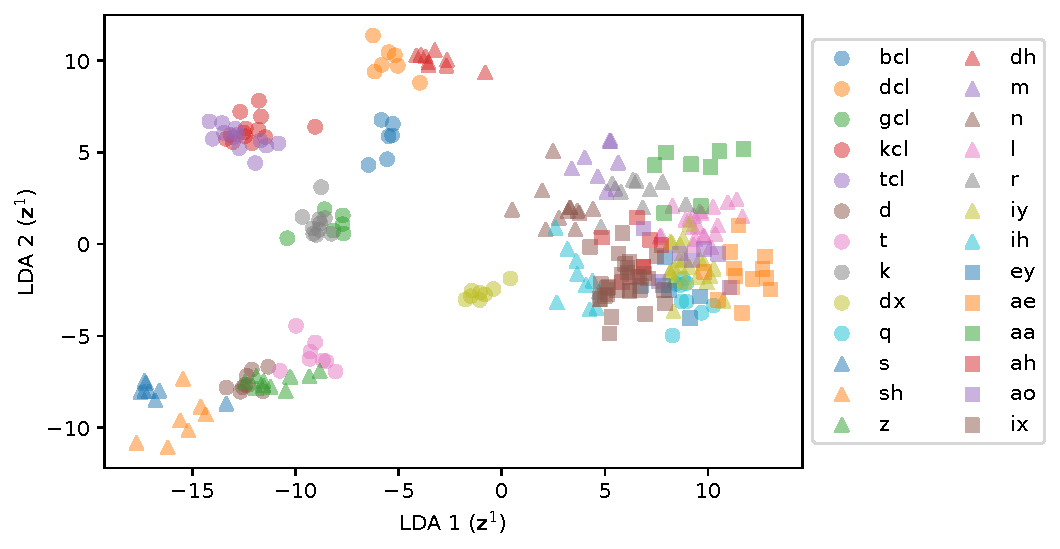
\includegraphics[width=0.555\textwidth]{paper_benchmarking/1xrnjn5y_speaker_phonemes_drw0_latent_0_samples_100_lda_linear_subspace.pdf}
    \hfill
    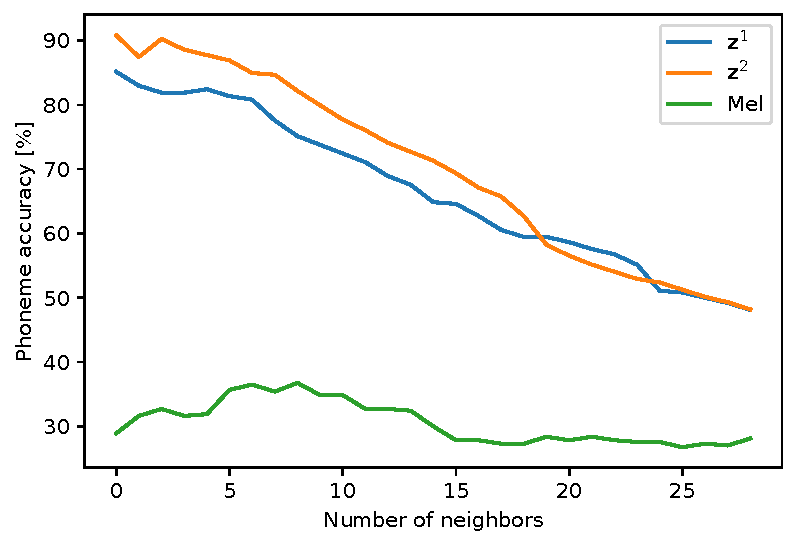
\includegraphics[width=0.425\textwidth]{paper_benchmarking/1xrnjn5y_speaker_phonemes_drw0_samples_100_knn_correct_fraction_model_vs_mel_30_neighbors_lda_subspace_5d.pdf}
    \caption[Clustering of phonemes in 2D subspace of CW-VAE latent space and KNN classification accuracy.]{
    (left) Clustering of phonemes in a 2D Linear Discriminant Analysis (LDA) subspace of a CW-VAE latent space ($\zb^{(1)}$).
    (right) Leave-one-out phoneme classification accuracy for a KNN classifier at different $K$ in a 5D LDA subspace of a CW-VAE latent space.
    }
    \label{fig: latent space phoneme and knn}
\end{figure*}
%

\paragraph{TIMIT}
For temporal resolutions of $s=1$, the deterministic autoregressive models yield the best likelihoods with WaveNet achieving $\SI{10.88}{bpf}$ on TIMIT as seen in \cref{tab: likelihoods timit} (left). 
Somewhat surprisingly, the LSTM baseline almost matches WaveNet with a likelihood of $\SI{11.11}{bpf}$ at $s=1$. However, due to being autoregressive in training, the LSTM trains considerably slower than the parallel convolutional WaveNet; something not conveyed by \cref{tab: likelihoods timit} (left). 
Notably, the VRNN and SRNN models achieve likelihoods close to that of WaveNet and the LSTM at around $\SI{11.09}{bpf}$. The STCN exhibited instability when trained at $s=1$ and tended to diverge.

At $s=64$, WaveNet and the LSTM yield significantly worse likelihoods than all LVMs separated by $\sim\SI{1}{bit}$.
The CW-VAE outperforms the VRNN and SRNN when configured with a hierarchy of latent variables. 
With a single layer of latent variables, the CW-VAE is inferior to both SRNN and VRNN but notably still better than the LSTM. 
These observations carry to $s=256$, where a multilayered CW-VAE outperforms the LSTM, VRNN and SRNN. 
The STCN yields the best results at both $s=64$ and $s=256$. 
For strides $s>1$, previous work has attributed the inferior performance of autoregressive models without latent variables, such as WaveNet and the LSTM, to the ability of LVMs to model intrastep correlations \parencite{lai_re-examination_2019}. 

Decreasing the resolution $s$ improves the likelihood for all LVMs. However, the best performing models, STCN and CW-VAE are not yet scalable to this regime for reasons related to numerical instability and computational infeasibility. This seems to indicate that LVMs may be able to outperform autoregressive models at $s=1$ in the future.
\paragraph{LibriSpeech}
On LibriSpeech (\cref{tab: likelihoods librispeech}), results are similar to TIMIT. The STCN achieves the best likelihood at $s=64$ and the CW-VAE surpasses WaveNet and the LSTM. 
\paragraph{Compression}
A connection can be made between the model likelihoods and the compression rates of audio compression algorithms. 
Lossy compression algorithms, such as MP3, exploit the dynamic range of human hearing to achieve 70-95\% reduction in bit rate \parencite{brandenburg_mpeg-2_1998} while lossless compression algorithms, such as FLAC, achieve 50-70\% reduction \parencite{coalson_free_2019} independent of audio content. 
% On LibriSpeech, FLAC achieves an overall compression to about 58\% of the original bit rate.
Although both the autoregressive models and the LVMs are lossy, their objective minimizes the amount of incurred loss. 
The best likelihoods reported in \cref{tab: likelihoods timit} (left) and \cref{tab: likelihoods librispeech} correspond to about a 30\% reduction in bit rate which indicates that there are significant gains in likelihood to be made in speech modeling.

\section{Phoneme recognition}\label{sec: phoneme recognition}
Although the likelihood is a practical metric for model comparison and selection, a high likelihood does not guarantee that a model has learned useful representations \parencite{huszar_is_2017}. 
For speech data, we would expect models to learn features related to phonetics which would make them useful for tasks such as automatic speech recognition (ASR). 
The Mel spectrogram is a well-established representation of audio designed for speech recognition and is predefined rather than learned. % \parencite{??}. Basic Correlates of the Auditory Stimulus, https://psycnet.apa.org/record/1951-07758-017, modern Mel scale https://ieeexplore.ieee.org/stamp/stamp.jsp?arnumber=1170013&casa_token=UIyQaj3tBRAAAAAA:GtttZedngBkaxVumjnXctc5zS50fptexPMiWhr-7gDrmIVq3JqJPnGCWYedoymb0X5JTGElmHf8&tag=1,
To assess the usefulness of the representations learned by the benchmarked models, we compare them to the highly useful Mel spectrogram on the task of phoneme recognition. 
Phonemes are fundamental units of speech that relate to how parts of words are pronounced (see also appendix~\cref{app: timit phoneme distributions}).
% rather than characters or words themselves (see also appendix~\cref{apsp: timit phoneme distributions}).

\paragraph{Quantitative}
We train an ASR model to recognize phonemes and compare its performance when using input representations obtained from different unsupervised models. 
For WaveNet and the LSTM, we use the hidden state as the representation. For all LVMs, we use the latent variable. For the hierarchical LVMs and WaveNet, we run the experiment using each possible representation and report only the best one here. 
We compare the learned representations to a log Mel spectrogram with 80 filter banks, hop length 64 and window size 128. 
We also compared to using raw PCM in vectors of 64 elements standardized to $[-1,1]$ but found that the ASR did not reliably converge at all which highlights the importance of input representation. 
The ASR model is a three-layered bidirectional LSTM with 256 hidden units. It is trained with the connectionist temporal classification (CTC) loss \parencite{graves_connectionist_2006} which lets it jointly learn to align and classify without using label alignments. 
We pre"=train all unsupervised models at $s=64$ on the full TIMIT training dataset excluding the validation data (3.7h) as in \cref{tab: likelihoods timit} (left). 
We then train the ASR model on all \SI{3.7}{h} as well as \SI{1}{h} and \SI{10}{m} subsets. We report results on the test set in terms of phoneme error rates (PER) in \cref{tab: phoneme recognition (PER)} (right).

As expected, Mel spectrogram performs well achieving 24.1\% PER using 3.7 hours of labeled data. However, the ASR trained on STCN representations outperforms the Mel spectrogram with a PER of 21.9\%. 
This indicates that unsupervised STCN representations are phonetically rich and potentially better suited for speech modeling than the engineered Mel spectrogram. 
When the amount of labeled data is reduced, LVM representations suffer slightly less than deterministic ones. WaveNet representations are interestingly outperformed by both the LSTM and all LVMs. 

% FH-VAE uses 3 layer bidirectional LSTM on 80 mel features. LSTM hidden state dim is 512 or 1024(?)
% FH-VAE https://arxiv.org/pdf/1709.07902.pdf
% [37] https://static.googleusercontent.com/media/research.google.com/da//pubs/archive/43905.pdf
% [13] https://www.cs.toronto.edu/~graves/asru_2013.pdf

\paragraph{Qualitative}
We qualitatively assess the learned latent representations for the CW-VAE. 
We infer the latent variables of all utterances by a single speaker from the TIMIT test set. We sample the latent sequence $100$ times to estimate the mean representation per timestep. We then compute the average latent representation over the duration of each phoneme using aligned phoneme labels. This approximately marginalizes variation during the phoneme. We use linear discriminant analysis (LDA) \parencite{fisher_use_1936} to obtain a low-dimensional linear subspace of the latent space. 
We visualize the resulting representations colored according to test set phoneme classes in \cref{fig: latent space phoneme and knn}. We note that many phonemes are separable in the linear subspace and that related phonemes such as ``s" and ``sh" are close.

We also show the average accuracy of a leave-one-out $k$-nearest-neighbor (KNN) classifier on the single left-out latent representation reduced with a 5-dimensional LDA as a function of the number of neighbors. 
We compare accuracy to a Mel-spectrogram averaged over each phoneme duration and LDA reduced. The spectrogram is computed with hop length set to 64, equal to $s_1$ for the CW-VAE, window size 256 and 80 Mel bins.
We see that both latent spaces yield significantly better KNN accuracies than the Mel features.


\section{Conclusion}
In this paper, we developed a benchmark for speech modeling with stochastic latent variable models (LVMs). 
We compared LVMs and deterministic autoregressive models on equal footing and found that LVMs achieve inferior likelihood compared to deterministic WaveNet and LSTM baselines. Surprisingly, the LSTM almost matched the popular WaveNet model. 
We saw that hierarchical LVMs, such as STCN and CW-VAE, outperformed non-hierarchical versions of themselves in ablation experiments as well as non-hierarchical LVMs such as VRNN and SRNN. This matches recent observations in the image domain. 
We noted that the STCN with an autoregressive decoder outperforms the non"=autoregressive CW-VAE, which we adapted to speech. 
Finally, we found that LVMs can learn latent representations that are useful for phoneme recognition and better than Mel spectrograms, which are tailored for the task, when identical models are trained on top of the representations.
While the best performing models are not yet scalable to the highest temporal resolution, these results indicate that they might improve upon deterministic models in the future. 


%%%%%%%%%%%%%%%%%%%%%%%%%%%%%%%%%%%%%%%%%%%%%%%%%%%%%%%%%%%%%%%%%%%%%%%%%%%%%%%

\section*{Acknowledgements}
This research was partially funded by the Innovation Fund Denmark via the Industrial PhD Programme (grant no.\@ 0153-00167B). JF and SH were funded in part by the Novo Nordisk Foundation (grant no.\@ NNF20OC0062606) via the Center for Basic Machine Learning Research in Life Science (MLLS, \hyperlink{https://www.mlls.dk}{https://www.mlls.dk}). JF was further funded by the Novo Nordisk Foundation (grant no.\@ NNF20OC0065611) and the Independent Research Fund Denmark (grant no.\@ 9131-00082B). SH was further funded by VILLUM FONDEN (15334) and the European Research Council (ERC) under the European Union's Horizon 2020 research and innovation programme (grant agreement no. 757360).

}
  % %!TEX root = ../thesis.tex

\chapter[benchmarking generative latent variable models for speech]{Benchmarking Generative Latent Variable Models for Speech}
\label{chp:paper-benchmarking-workshop}
\ifthenelse{\equal{\skippapers}{true}}{}{

\section{Abstract}
Stochastic latent variable models (LVMs) achieve state-of-the-art performance on natural image generation but are still inferior to deterministic models on speech. In this paper, we develop a speech benchmark of popular temporal LVMs and compare them against state-of-the-art deterministic models. We report the likelihood, which is a much used metric in the image domain, but rarely, or incomparably, reported for speech models. To assess the quality of the learned representations, we also compare their usefulness for phoneme recognition. Finally, we adapt the Clockwork VAE, a state-of-the-art temporal LVM for video generation, to the speech domain. Despite being autoregressive only in latent space, we find that the Clockwork VAE can outperform previous LVMs and reduce the gap to deterministic models by using a hierarchy of latent variables.


%%%%%%%%%%%%%%%%%%%%%%%%%%%%%%%%%%%%%%%%%%%%%%%%%%%%%%%%%%%%%%%%%%%%%%%%


\section{Introduction}
Since their introduction, temporal latent variable models (LVMs) for speech \parencite{chung_recurrent_2015, fraccaro_sequential_2016} based on the variational autoencoder (VAE,  \textcite{kingma_autoencoding_2014, rezende_stochastic_2014}) have seen little development compared to their image domain counterparts. While LVMs now achieve superior likelihoods on images compared to deterministic models \parencite{child_very_2021,sinha_consistency_2021,kingma_variational_2021}, they are still inferior to deterministic models such as WaveNet on speech \parencite{oord_wavenet_2016}.
Development in the image domain has been driven by established likelihood benchmarks, but in the speech domain, likelihoods are often not reported \parencite{oord_wavenet_2016, hsu_unsupervised_2017, oord_neural_2018} or are incomparable due to subtle differences in the chosen data distributions \parencite{chung_recurrent_2015, fraccaro_sequential_2016, hsu_unsupervised_2017, aksan_stcn_2019}. 
This makes it hard to develop explicit likelihood models for speech.

In this paper, we develop a likelihood benchmark for recent temporal LVMs and compare to deterministic counterparts including WaveNet. We introduce a hierarchical LVM without autoregressive decoder and finally evaluate the learned representations for phoneme recognition. We find that 
(i) LVMs achieve likelihoods superior to WaveNet at low temporal resolution, 
(ii) LVMs with autoregressive decoders achieve better likelihoods than a non"=autoregressive LVM, 
(iii) LVM likelihoods improve when using hierarchies of latent variables as also seen for images and, 
(iv) LVM representations are as good or better than Mel spectrograms for phoneme recognition.


\begin{figure*}[t!]
    \centering
    \begin{multicols}{5}
    \setlength\columnsep{0mm}
    \resizebox{!}{4.5cm}{
    \begin{tikzpicture}
        \node[obs] (x_t) {$\vx_t$};
        
        % \node[above=0.75cm of x_t, xshift=0cm] (cap1) {$p(\vx_t|\vx_{<t})$};
        \node[above=0.3cm of x_t] (caption) {LSTM};
        
        \node[det,below=2.55cm of x_t] (d_t) {$\vd_{t}$};
        \node[det,left=0.75cm of d_t] (d_tm1) {$\vd_{t-1}$};
        \node[obs,below=0.75cm of d_t] (x_tm1) {$\vx_{t-1}$};
        
        \edge[deterministic-skip-color]{x_tm1}{d_t};
        \edge[deterministic-skip-color]{d_t}{x_t};
        \edge[deterministic-skip-color]{d_tm1}{d_t};
        \edge[draw=white,bend right]{d_t}{x_t};  % for identical width to others
    \end{tikzpicture}
    }
    \\
    \resizebox{!}{4.5cm}{
    \begin{tikzpicture}
        \node[obs] (x_t) {$\vx_t$};
        
        % \node[above=0.75cm of x_t, xshift=0cm] (cap1) {$p(\vx_t|\vz_{\leq t},\vx_{<t}) p(\vz_t|\vx_{<t},\vz_{<t})$};
        \node[above=0.3cm of x_t] (caption) {VRNN};
        
        \node[latent,below=0.75cm of x_t] (z_t) {$\vz_t$};
        \node[latent,left=0.75cm of z_t] (z_tm1) {$\vz_{t-1}$};
        
        \node[det,below=0.75cm of z_t] (d_t) {$\vd_{t}$};
        \node[det,below=0.75cm of z_tm1] (d_tm1) {$\vd_{t-1}$};
        \node[obs,below=0.75cm of d_t] (x_tm1) {$\vx_{t-1}$};
        
        \edge[deterministic-skip-color]{x_tm1}{d_t};
        \edge[]{d_t}{z_t};
        \edge[]{z_tm1}{d_t};
        \edge[deterministic-skip-color]{d_tm1}{d_t};
        \edge[]{z_t}{x_t};
        \edge[deterministic-skip-color,bend right]{d_t}{x_t};
    \end{tikzpicture}
    }
    \\
    \resizebox{!}{4.5cm}{
    \begin{tikzpicture}
        \node[obs] (x_t) {$\vx_t$};
        
        % \node[above=0.75cm of x_t, xshift=0cm] (cap1) {$p(\vx_t|\vz_{\leq t},\vx_{<t}) p(\vz_t|\vx_{<t},\vz_{<t})$};
        \node[above=0.3cm of x_t] (caption) {SRNN};
        
        \node[latent,below=0.75cm of x_t] (z_t) {$\vz_t$};
        \node[latent,left=0.75cm of z_t] (z_tm1) {$\vz_{t-1}$};
        
        \node[det,below=0.75cm of z_t] (d_t) {$\vd_{t}$};
        \node[det,below=0.75cm of z_tm1] (d_tm1) {$\vd_{t-1}$};
        \node[obs,below=0.75cm of d_t] (x_tm1) {$\vx_{t-1}$};
        
        \edge[deterministic-skip-color]{x_tm1}{d_t};
        \edge[]{d_t}{z_t};
        \edge[]{z_tm1}{z_t};
        \edge[deterministic-skip-color]{d_tm1}{d_t};
        \edge[]{z_t}{x_t};
        \edge[deterministic-skip-color,bend right]{d_t}{x_t};
    \end{tikzpicture}
    }
    \\
    \resizebox{!}{4.5cm}{
    \begin{tikzpicture}
        \node[obs] (x_t) {$\vx_t$};
        % \node[above=0.75cm of x_t, xshift=0cm] (cap1) {$p(\vx_t|\vz_t,\vx_{t-r:t-1})$};
        \node[above=0.3cm of x_t] (caption) {STCN};
        
        \node[latent,below=0.75cm of x_t] (z_t) {$\vz_t$};
        \node[left=0.025cm of z_t] (dots) {$\cdots$};
        \node[latent,left=0.75cm of z_t] (z_tmr) {$\vz_{t-r'}$};
        
        \node[det,below=0.75cm of z_t] (d_t) {$\vd_{t}$};
        \node[obs,below=0.75cm of d_t] (x_tm1) {$\vx_{t-1}$};
        \node[left=0.025cm of x_tm1] (dots) {$\cdots$};
        \node[obs,left=0.75cm of x_tm1] (x_tmr) {$\vx_{t-r}$};
        
        \edge[]{x_tm1}{d_t};
        \edge[]{x_tmr}{d_t};
        \edge[]{d_t}{z_t};
        \edge[]{z_t}{x_t};
        \edge[]{z_tmr}{x_t};
        \edge[draw=white,bend right]{d_t}{x_t};  % for identical width to others 
    \end{tikzpicture}
    }
    \\
    \resizebox{!}{4.5cm}{
    \begin{tikzpicture}
        \node[obs] (x_t) {$\vx_t$};%

        % \node[above=0.75cm of x_t, xshift=0cm] (cap1) {$p(\vx_t|\vz_{\leq t}) p(\vz_t|\vz_{<t})$};
        \node[above=0.3cm of x_t] (caption) {CW-VAE};
        
        \node[latent,below=0.75cm of x_t] (z_t) {$\vz_t$};
        \node[latent,left=0.75cm of z_t] (z_tm1) {$\vz_{t-1}$};
        
        \node[det,below=0.75cm of z_t] (d_t) {$\vd_{t}$};
        \node[det,below=0.75cm of z_tm1] (d_tm1) {$\vd_{t-1}$};
        \node[obs,below=0.75cm of d_t,draw=white,fill=white] (x_tm1) {};
        
        \edge[]{d_t}{z_t};
        \edge[bend right]{d_t}{x_t};
        \edge[]{z_tm1}{d_t};
        \edge[]{d_tm1}{d_t};
        \edge[]{z_t}{x_t};
    \end{tikzpicture}
    }
    \end{multicols}
\caption{
Generative models of an LSTM, VRNN, SRNN, STCN and CW-VAE for a single time step. The STCN and CW-VAE are illustrated with a single latent variable. 
Red arrows indicate purely deterministic paths from the output $\vx_t$ to previous input $\vx_{<t}$ without passing a stochastic node. 
We provide additional graphical illustrations including inference models in \cref{app: additional graphical models}.
}
\label{fig: autoregressive vrnn srnn cwvae 1L graphs}
\end{figure*}

\paragraph{Scope and related work} 
At a high level, this benchmark brings order to LVM model comparisons for speech and also provides useful reference implementations of the models\footnote{\texttt{ \href{https://github.com/JakobHavtorn/benchmarking-lvms}{github.com/JakobHavtorn/benchmarking-lvms}}}. 
An extended version of this paper is available at \href{https://arxiv.org/abs/2202.12707}{arXiv:2202.12707}.
LVMs based on the VAE are of interest due to their ability to learn an approximate posterior distribution over latent variables. This makes them useful beyond generation for e.g. semi"=supervised learning \parencite{kingma_semi-supervised_2014} and anomaly detection \parencite{havtorn_hierarchical_2021}. 
In this paper, we focus on the VRNN \parencite{chung_recurrent_2015}, SRNN \parencite{fraccaro_sequential_2016} and STCN \parencite{aksan_stcn_2019} since they are similar to the original VAE framework. 
We exclude some related work from the benchmark. Specifically, the FH-VAE \parencite{hsu_unsupervised_2017} adds a global latent variable but we exclude it due to it's segmentation of the training data. We also exclude Z-forcing \parencite{goyal_zforcing_2017} which resembles the SRNN, but deviates from maximum likelihood training by using an auxiliary loss. We exclude the VQ-VAE \parencite{oord_neural_2018} which is a hybrid LVM and autoregressive model, since it uses a quantized latent space. Finally, we exclude the Stochastic WaveNet \parencite{lai_stochastic_2018} which is similar, but inferior, to the STCN \parencite{aksan_stcn_2019}.

All selected models have autoregressive generative models. We therefore formulate and benchmark a novel temporal LVM which does not use an autoregressive decoder. We do so by adapting the hierarchical Clockwork Variational Autoencoder \parencite{saxena_clockwork_2021}, originally proposed for video generation, to speech.
Before presenting the results, we provide a brief survey of existing LVMs for speech in a coherent notation. 

\section{Models}
\paragraph{Sequential deep latent variable models}
The models we consider are all sequential deep latent variable models trained with variational inference and the reparameterization trick \parencite{kingma_autoencoding_2014}.
The input is a variable-length sequence $\vx = \vx_{1:T} = \left(\vx_1, \vx_2, \dots, \vx_{T}\right)$ with $\vx_t\in\mathbb{R}^{D_x}$. 
The models first encode $\vx_{1:T}$ to a temporal posterior distribution $q(\vz|\vx)$ and sample a latent representation $\vz_{1:T}$ where $\vz_t\in\mathbb{R}^{D_z}$. This is then used to reconstruct the input while the posterior distribution is regularized to be close to a prior distribution $p(\vz_t|\cdot)$ where the dot indicates that it may depend on latent and observed variables at previous time steps, $\vz_{<t}$ and $\vx_{<t}$ where $\vz_{<t} := \left( \vz_1, \vz_2, \dots, \vz_{t-1} \right)$. 
The models are trained to maximize a lower bound $\mathcal{L}(\thetab,\phib;\vx)$ on the marginal likelihood $\log p_\thetab(\vx)$,
\begin{equation}
    \log p_\thetab(\vx) = \log \int p_\thetab(\vx,\vz) \, \mathrm{d}\vz  \geq \int q_\phib(\vz|\vx) \log \frac{p_\thetab(\vx|\vz)p(\vz)}{q_\phib(\vz|\vx)}  \, \mathrm{d}\vz \equiv \mathcal{L}(\thetab,\phib;\vx)  \enspace , \label{eq: elbo}
\end{equation}
where $\thetab$ are parameters of the generative model and $q_\phib(\vz|\vx)$ is the variational approximation to the true posterior.
Graphical illustrations of the models can be seen in \cref{fig: autoregressive vrnn srnn cwvae 1L graphs} and appendix~\cref{app: additional graphical models}.

\paragraph{Variational recurrent neural network (VRNN)}
The VRNN \parencite{chung_recurrent_2015} is essentially a VAE per timestep. As seen in \cref{fig: autoregressive vrnn srnn cwvae 1L graphs}, it is conditioned on the hidden state of a Gated Recurrent Unit (GRU, \textcite{cho_properties_2014}) with state transition $\vd_{t} = f([\vx_{t-1}, \vz_{t-1}], \vd_{t-1})\in\mathbb{R}^{D_d}$ where $[\cdot, \cdot]$ denotes concatenation. 
The joint and variational posterior distributions are given by
\begin{equation}
    p(\vx,\vz) = \prod_{t=1}^{T} p(\vx_t|\vx_{<t},\vz_{\leq t}) p(\vz_t|\vx_{<t},\vz_{<t}) \, ,\quad 
    q(\vz|\vx) = \prod_{t=1}^{T} q(\vz_t|\vx_{\leq t},\vz_{<t}) \enspace . \label{eq: vrnn joint and inference}
\end{equation}
%
\paragraph{Stochastic recurrent neural network (SRNN)}
The SRNN \parencite{fraccaro_sequential_2016} is similar to the VRNN and its joint can be written as in \eqref{eq: vrnn joint and inference}. Contrary to the VRNN, the SRNN has GRU state transitions that are independent of $\vz_{1:T}$ such that $\vd_{t} = f(\vx_{t-1}, \vd_{t-1})$. Furthermore, the SRNN conditions on the full observed sequence for inference, $q(\vz_t|\vx_{1:T},\vz_{t-1})$ via a second GRU with transition $\va_t = g([\vx_t,\vd_t], \va_{t+1})$. Then $\vz_t$ is inferred from $\va_t$ and $\vz_{t-1}$. This better approximates the true posterior which can be shown to depend on the full observed sequence \parencite{bayer_mind_2021}. 

\paragraph{Stochastic temporal convolutional network (STCN)}
Contrary to VRNN and SRNN, the latent variables of the STCN are conditionally independent given $\vx_{1:T}$ since there are no transition functions connecting them over time.
Instead, a latent $\vz_t^{(l)}$ at layer $l$ is conditioned on the latent variable above it $\vz^{(l+1)}_t$ and a window of $\vx_{1:T}$ defined by $\mathcal{R}_t^{(l)} = \cbra{t-r_l+1,\dots,t}$ via a WaveNet encoder with receptive field $r_l$ at layer $l$ \parencite{oord_wavenet_2016}. The joint and variational posterior are, 
\begin{equation}
\resizebox{.99\textwidth}{!}{%
$
p(\vx,\vz) = \prod\limits_{t=1}^{T} p(\vx_t|\vz_{{\scriptscriptstyle \mathcal{R}}_{t}}) \prod\limits_{l=1}^{L} p(\vz^{(l)}_{t}|\vx_{\scriptscriptstyle\mathcal{R}_{t-1}^{(l)}},\vz^{(l+1)}_{t}) \, , \,\, q(\vz|\vx) = \prod\limits_{t=1}^{T}\prod\limits_{l=1}^{L} q(\vz_{t}^{(l)}|\vx_{\scriptscriptstyle\mathcal{R}_{t}^{(l)}},\vz_t^{(l+1)}) \, , \nonumber
$
}
\label{eq: stcn joint and inference}
\end{equation}
where $\vz_t^{(L+1)}:=\emptyset$ and $\vz=\vz_{1:T}^{(1:L)}$ for notational convenience and inference is done top-down \parencite{sonderby_ladder_2016}. The observation model $p(\vx_t|\vz^{(1:L)}_{{\scriptscriptstyle \mathcal{R}}_{t}^{(1)}})$ is also parameterized by a WaveNet. 

\paragraph{Clockwork variational autoencoder (CW-VAE)}
The CW-VAE \parencite{saxena_clockwork_2021} is a hierarchical LVM originally introduced for video generation. As seen in figure~\cref{fig: autoregressive vrnn srnn cwvae 1L graphs}, it is autoregressive in the latent space but not in the observed space, contrary to the VRNN, SRNN and STCN. Additionally, each latent variable is updated only every $s_l$ timesteps, where $s_l$ is a layer-dependent stride and $s_1<s_2<\dots<s_L$. 
We define $\mathcal{J}_t := \{ l \,|\, t\in\mathcal{T}_l \}$ and $\mathcal{T}_l := \{t \in \bra{1,T} \,|\, (t-1)\,\text{mod}\, s_l = 0\}$. Then,
\begin{equation}
\resizebox{0.99\textwidth}{!}{%
$
    p(\vx,\vz) = 
    \prod\limits_{t=1}^{T} p(\vx_t | \vz_t^{(1)})
    \prod\limits_{l\in\mathcal{J}_t} p(\vz_t^{(l)} | \vz_{t-s_l}^{(l)}, \vz_t^{(l+1)}) \, , \,\,
    q(\vz | \vx) = \prod\limits_{t=1}^T \prod\limits_{l\in\mathcal{J}_t} q(\vz_t^{(l)} | \vz_{t-s_l}^{(l)}, \vz_t^{(l+1)}, \vx_{t:t+s_l}) \, .
    \nonumber
$
}
\label{eq: cwvae joint and inference}
\end{equation}
The original encoder and decoder are not directly applicable to speech, since the sampling rates of speech are much higher than those of video (e.g. $\SI{16000}{Hz}$ compared to  $\SI{30}{Hz}$). Hence, we use a convolutional ladder network similar to the STCN for inference and downsample the waveform.

\paragraph{Output distribution} Recent work on LVMs for speech modeling, including those considered here, often uses a Gaussian output distribution \parencite{chung_recurrent_2015, fraccaro_sequential_2016,hsu_unsupervised_2017,lai_stochastic_2018,aksan_stcn_2019,zhu_s3vae_2020}. 
Since audio is a naturally continuous signal, this may seem like an appropriate modeling choice. However, common audio datasets are sampled at bit-depths of $\SI{16}{bit}$ (TIMIT, \citealt{garofolo_timit_1993}; LibriSpeech, \citealt{panayotov_librispeech_2015}). This results in a quantization gap between unique values of $1\times10^{-5}$ which increases the risk of an ill-posed problem by a likelihood that is unbounded from above unless the variance is lower bounded \parencite{mattei_leveraging_2018}. As a result, \emph{reported likelihoods can be sensitive to hyperparameter settings and be hard to compare}. We discuss this phenomenon further in appendix~\cref{app: gaussian likelihood unboundedness discussion}.

In this work, we therefore benchmark models using a discretized mixture of logistics (DMoL) as output distribution. The DMoL was introduced for image modeling with autoregressive models \parencite{salimans_pixelcnn_2017} but has become standard in other generative models \parencite{maaloe_biva_2019, vahdat_nvae_2020, child_very_2021}. Although continuous distributions can be used if the data is dequantized \parencite{dinh_nice_2015,theis_note_2016,ho_flow_2019}, we do not consider this option here.


\section{Speech modeling benchmark}

\input{tables/results}

\paragraph{Data}
We train models on TIMIT \parencite{garofolo_timit_1993} and randomly sample 5\% of the training split for validation. 
Both input and target are $\mu$-law PCM standardized to $\bra{-1, 1}$. 
We report on LibriSpeech \parencite{panayotov_librispeech_2015} and linear PCM in appendix~\cref{app: additional likelihood results appendix}. We further describe datasets in appendix~\cref{app: dataset details}.

\paragraph{Likelihood}
We report likelihoods in units of bits per frame (bpf; lower is better) as this yields a more interpretable likelihood that has connections to information theory and compression \parencite{shannon_mathematical_1948, townsend_practical_2019} compared to total likelihood in nats. For LVMs, we report the one-sample ELBO. The likelihoods can be seen in \cref{tab: likelihoods timit}. We describe how to convert to bpf in appendix~\cref{app: likelihood in bits per frame}.

\paragraph{Models}
We configure WaveNet, VRNN, SRNN, STCN and CW-VAE as in the original papers  with the choices described here. Specifically, WaveNet uses ten layers, five blocks and $D_c=96$ channels. VRNN and SRNN use latent dimension $D_z=256$ and an equal number of hidden units. The STCN is in the dense configuration and uses 256 convolution channels, $L=5$ layers and latent variables of dimensions $16, 32, 64, 128, 256$ from the top down. We also run a one-layered ablation with the same architecture but only one latent variable of dimension $256$ at the top. The CW-VAE has $L=1$ or $2$ latent variables of dimension 96 equal to the number of convolution channels and we let $s$ refer to $s_1$ and set $s_2=8s_1$. We also train an LSTM baseline \parencite{hochreiter_long_1997} configured similar to the VRNN.
%
All models use a 10 component DMoL output distribution. All LVMs use diagonal covariance Gaussian priors and posteriors. We train and evaluate models with waveforms stacked similar to previous work \parencite{chung_recurrent_2015, fraccaro_sequential_2016, aksan_stcn_2019} with stack sizes of $s=1$, $s=64$ and $s=256$. 
Finally, we evaluate a per-frame discrete uniform distribution and a two-component DMoL fitted to the training set to estimate worst case performance. 
We further describe models and training in appendix~\cref{app: model architectures} and \cref{app: training details} and provide results with a Gaussian output distribution in appendix~\cref{app: additional likelihood results appendix}. 

\paragraph{Results}
We present the model likelihoods for $s=1$ and $64$ in \cref{tab: likelihoods timit} and for $s=256$ in appendix~\cref{app: additional likelihood results appendix}. It is clear that deterministic autoregressive models are superior to LVMs at $s=1$, but inferior to them at $s=64$ and $256$. For strides $s>1$, previous work has attributed the inferior performance of autoregressive models without latent variables to the ability of LVMs to model intra-step correlations \parencite{lai_re-examination_2019}. It should be noted that at $s=1$, the STCN was numerically unstable and that the CW-VAE was computationally infeasible to train.
%
Surprisingly, the simple LSTM performs almost on par with WaveNet. The autoregressive STCN is the best-performing LVM. For both CW-VAE and STCN, increasing the number of latent variables in the hierarchy improves performance, similar to results in the image domain. 
%The best likelihoods correspond to about a 30\% reduction in bit rate which is inferior to FLAC indicating that significant gains in likelihood might be possible. 
The best performing LVMs, STCN and CW-VAE, are not yet scalable to $s=1$ resolution where the highest likelihoods are achieved. Hence, LVMs may be able to outperform autoregressive models at $s=1$ in the future.

\paragraph{Phoneme recognition}
Although the likelihood is a practical metric for model comparison, a high likelihood does not guarantee that a model has learned useful representations \parencite{huszar_is_2017}. To assess the usefulness of the representations, we train a model to recognize phonemes on the TIMIT data. We compare the phoneme error rate (PER) of the model when using input representations obtained from different unsupervised models, trained on the full TIMIT dataset (3.7h) at $s=64$, as in \cref{tab: likelihoods timit}, and when using a Mel spectrogram (80 filterbanks, hop length 64, window size 128). The recognition model is a three-layered bidirectional LSTM with 256 hidden units. It is trained with the connectionist temporal classification (CTC) loss \parencite{graves_connectionist_2006}. We report the PER in \cref{tab: phoneme recognition (PER)}.

As expected, Mel spectrograms perform well achieving 24.1\% PER using 3.7 hours of labeled data. However, the ASR trained on STCN representations outperforms the Mel spectrogram with a PER of 21.9\%. 
This indicates that unsupervised STCN representations are phonetically rich and potentially better suited for speech modeling than the engineered Mel spectrogram. 
When the amount of labeled data is reduced, LVM representations suffer slightly less than deterministic ones. Interestingly, representations from WaveNet are outperformed by all LVMs and the LSTM. 


\section*{Acknowledegments}
This research was partially funded by the Innovation Fund Denmark via the Industrial PhD Programme (grant no.\@ 0153-00167B). JF and SH were funded in part by the Novo Nordisk Foundation (grant no.\@ NNF20OC0062606) via the Center for Basic Machine Learning Research in Life Science (MLLS, \hyperlink{https://www.mlls.dk}{https://www.mlls.dk}). JF was further funded by the Novo Nordisk Foundation (grant no.\@ NNF20OC0065611) and the Independent Research Fund Denmark (grant no.\@ 9131-00082B). SH was further funded by VILLUM FONDEN (15334) and the European Research Council (ERC) under the European Union’s Horizon 2020 research and innovation programme (grant agreement no. 757360).

}

%!TEX root = ../thesis.tex

\chapter[self-supervised speech representation learning: a review]{Self-Supervised Speech Representation Learning: A Review}
\label{chp:review}

% no-op commands
\newcommand{\edit}[1]{#1}
\newcommand{\ci}[1]{#1}
\newcommand{\red}[1]{#1}
\newcommand{\TNS}[1]{#1}
\newcommand{\kl}[1]{#1}
\newcommand{\abdo}[1]{#1}


\section*{Abstract}
Although supervised deep learning has revolutionized speech and audio processing, it has necessitated the building of specialist models for individual tasks and application scenarios. It is likewise difficult to apply this to dialects and languages for which only limited labeled data is available. 
Self-supervised representation learning methods promise a single universal model that would benefit a wide variety of tasks and domains. 
Such methods have shown success in natural language processing and computer vision domains, achieving new levels of performance while reducing the number of labels required for many downstream scenarios. Speech representation learning is experiencing similar progress in three main categories: generative, contrastive, and predictive methods. 
Other approaches rely on multi-modal data for pre-training, mixing text or visual data streams with speech. 
Although self-supervised speech representation is still a nascent research area, it is closely related to acoustic word embedding and learning with zero lexical resources, both of which have seen active research for many years. 
This review presents approaches for self-supervised speech representation learning and their connection to other research areas. 
Since many current methods focus solely on automatic speech recognition as a downstream task, we review recent efforts on benchmarking learned representations to extend the application beyond speech recognition. 

% TODO (JDH): Revise all references in this chapter
%!TEX root = ../thesis.tex


\section{Introduction}

\begin{figure}
    \centering
    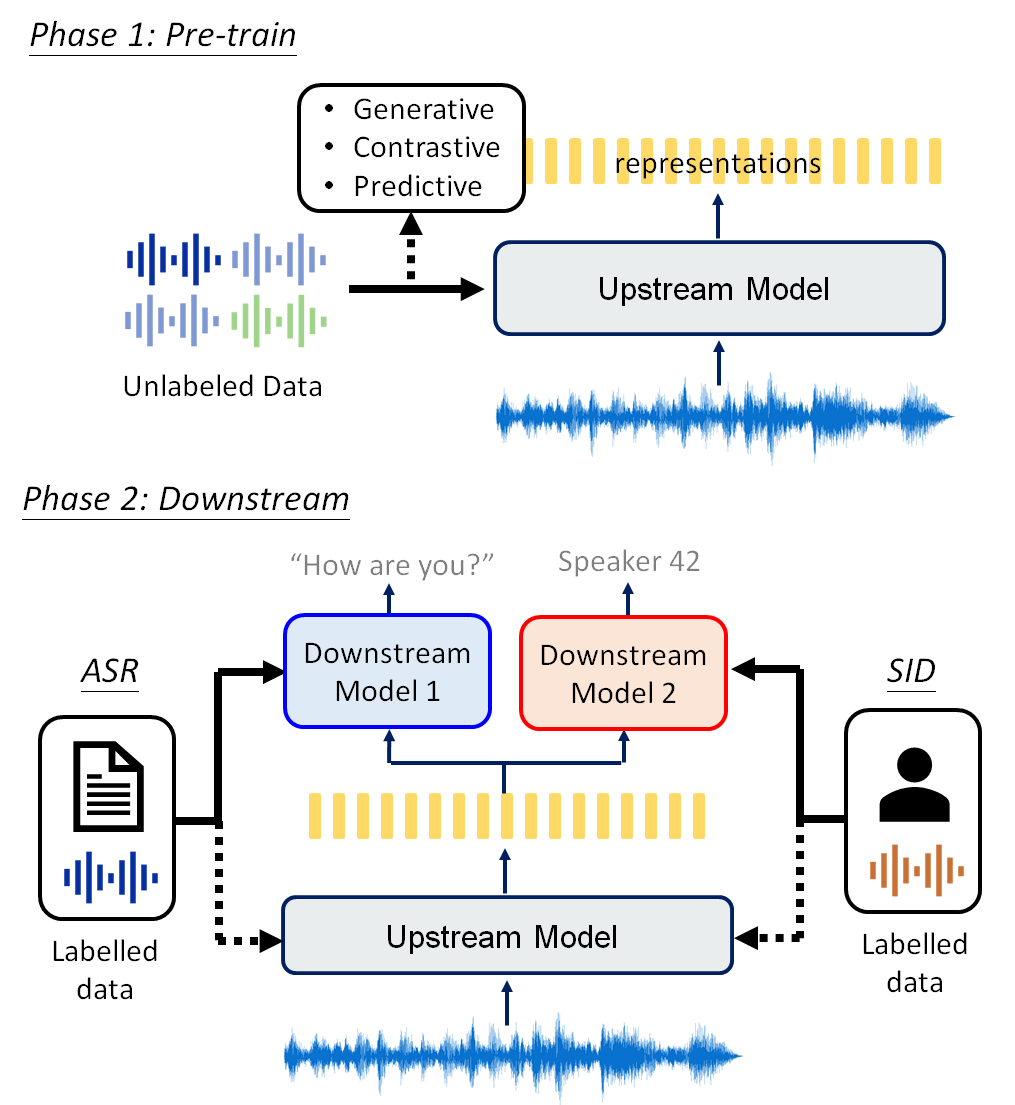
\includegraphics[width=0.80\textwidth]{paper_review/SSL_framework.png}
	 \caption{Framework for using self-supervised representation learning in
	 downstream applications.}
    \label{fig:SSL_framework}
\end{figure}


Over the past decade, deep learning approaches have revolutionized speech processing
through a giant leap in performance, enabling various real-world applications.
Supervised learning of deep neural networks has been the cornerstone of this
transformation, offering impressive gains for scenarios rich in labeled
% data~\cite{lecun_deep_2015}. 
% data~\cite{lecun_deep_2015, hinton_deep_2012}. 
% data~\cite{bourlard_connectionist_1994}. 
% data~\cite{lecun_deep_2015,bourlard_connectionist_1994}. 
data~\cite{lecun_deep_2015,hinton_deep_2012,bourlard_connectionist_1994}. 
Paradoxically, this heavy reliance on supervised learning has restricted progress in
languages and domains that do not attract the same level of labeling
investment. 

To overcome the need for labeled data, researchers have explored approaches that use
unpaired audio-only data to open up new industrial speech use-cases and
low-resource languages~\cite{kemp_unsupervised_1999, lamel_lightly_2002, ma_unsupervised_2006}. Inspired by how
children learn their first language through listening and interacting with
family and surroundings, scientists seek to use raw waveforms and
spectral signals to learn speech representations that capture low-level
acoustic events, lexical knowledge, all the way to syntactic and semantic
information. These learned representations are then used for target downstream
applications requiring a minimal number of labeled data~\cite{hinton_learning_2007,
lecun_tutorial_2006, bengio_representation_2013}. 
Formally, representation learning refers to algorithms for extracting latent
features that capture the underlying explanatory factors for the observed
input~\cite{bengio_representation_2013}. 

Representation learning approaches are generally considered examples of \textit{unsupervised
learning}, which refers to the family of machine learning methods that discover
naturally occurring patterns in training samples for which there are no pre-assigned
labels or scores~\cite{jordan_machine_2015}. 
The term ``unsupervised'' is used to distinguish this family of methods from
``supervised'' approaches, which assign a label to each training sample, and
``semi-supervised'' approaches, which utilize a small number of training samples
with labels to guide learning using a larger volume of unlabeled samples.
Examples of unsupervised learning techniques include $k$-means clustering~\cite{gray_vector_1984}, mixture models~\cite{jordan_hierarchical_1994}, autoencoders~\cite{hinton_autoencoders_1994},
and non-negative matrix factorization~\cite{lee_learning_1999}. 
\textit{Self-supervised learning} (SSL) is a fast-growing subcategory of
unsupervised learning approaches, which are techniques that utilize
information extracted from the input data itself as the label to learn
representations useful for 
downstream tasks. {\color{black} For example, unsupervised $k$-means clustering doesn't adhere to this definition of self-supervision since it iteratively minimizes the within-cluster variance during learning.}
In this review, we
focus on self-supervised learning approaches.

\Cref{fig:SSL_framework} outlines self-supervised representation learning in
relation to downstream applications. 
There are two stages in this framework.
In the first stage, we use SSL to pre-train a \textit{representation model},
also called an \textit{upstream model} or a \textit{foundation model}.
In the second stage, downstream tasks use either the learned
representation from the frozen model, or fine-tune the entire pre-trained model
in a supervised phase~\cite{hinton_reducing_2006}. 
Automatic speech recognition (ASR) and speaker identification (SID) are 
examples of downstream applications in \cref{fig:SSL_framework}.

It is considered desirable for learned speech representations to be
disentangled, invariant, and hierarchical.
Since spoken utterances contain much richer information than the corresponding text
transcriptions---e.g., speaker identity, style, emotion, surrounding noise, and
communication channel noise---it is important to learn representations that
disentangle these factors of variation. Furthermore, invariance of the learned
features to changes in background noise and in the communication channel ensures
stability with respect to downstream application scenarios. Learning feature
hierarchies at the acoustic, lexical, and semantic levels supports applications
with different requirements. For instance, whereas a speaker identification task
benefits from a low-level acoustic representation, a speech
translation task requires a more semantic representation of the input
utterance. 

Due to the popularity of SSL, reviews have been published about the
technology in general~\cite{bommasani_opportunities_2021,ericsson_selfsupervised_2022,liu_selfsupervised_2021} as well as its application to natural language processing (NLP)~\cite{rogers_primer_2020,liu_pretrain_2021,xia_which_2020,qiu_pretrained_2020} and computer vision (CV)~\cite{jing_selfsupervised_2021}. Recently, a brief overview with a general focus on speech representation learning was published \cite{borgholt_brief_2022}. 
However, none of these overviews focus exclusively on SSL for speech processing. Since the speech signal differs greatly from image and text inputs, many  theories  and technologies have been developed to address the unique challenges of speech. 
One review addresses speech representation learning based on deep learning models~\cite{latif_deep_2021}, but does not address recent developments in self-supervised learning. This motivates this overview of speech SSL.


The structure of this paper is arranged as follows. \Cref{sec:thirdwave}
briefly reviews the history of speech representation learning, and
\cref{sec:approach} reviews current speech SSL models.
\Cref{section:benchmark} surveys SSL datasets and benchmarks, 
and discusses and compares results from different works. \Cref{analysis}
analyzes successful SSL approaches and offers insights into the
importance of technological innovations. \Cref{sec:zero} reviews 
zero-resource downstream tasks that utilize SSL. 
Finally, \cref{sec:conclusion} summarizes the paper and suggests 
future research directions.



%!TEX root = ../thesis.tex

\section{Historical Context of Representation Learning}

\label{sec:thirdwave}

In this section we present the historical background of the current surge in
self-supervised representation learning methods in the context of two previous
waves of research work in the 1990s and 2000s. The discussed approaches go
beyond speech to describe the overall landscape of machine learning development during the
past few decades.

\subsection{Clustering and mixture models}

Initial research in learning latent speech and audio representations involved
simple models in which the training data likelihood was optimized directly
or via the expectation--maximization (EM) algorithm.

Early work used simple clustering methods. For example, in work such
as \cite{rabiner_considerations_1979,wilpon_modified_1985}, word patterns were clustered
semi-automatically using techniques such as k-means, after which isolated words
were recognized by finding the training cluster closest to 
  the test data.

Through time, modeling techniques improved such that subword units were
represented by Gaussian mixture models (GMMs) \cite{gauvain_maximum_1994}, which facilitated
the modeling of more variability in the input data. GMMs were first built for
context-independent phonemes; state-clustering 
algorithms~\cite{young_state_1994} then resulted in GMMs for context-dependent phonemes. 
Each latent component of these mixture models acted as a template of a
prototypical speech frame, 
making it difficult to handle 
large volumes of data with diverse characteristics. 
Furthermore, dynamical models like hidden Markov models (HMMs)~\cite{bell_adaptation_2021}
allowed for the processing of continuous speech rather than just isolated word
recognition. These generative GMM and HMM models were trained by maximizing the
likelihood of data given the model, which could be accomplished in either an
unsupervised or a supervised manner.

Another line of research focused on extracting speech features from generative
models. The main objective here was to render the knowledge learned by generative
models accessible to discriminative downstream classifiers, or to map
variable-length sequences to fixed-length representations. Feature vectors
were derived from the parameters of trained GMM models. In the case of {\em
Fisher vectors}, the features were the normalized gradients of the
log-likelihood with respect to the model parameters (mixture weights, means, and
variances) of the Gaussian mixtures. An extension of this approach (likelihood
ratio score space) used the derivative of the log-likelihood ratio of two
models, e.g., a background model and a foreground model. Examples of their use
in speech processing include speech recognition~\cite{smith_speech_2001,venkataramani_support_2003} and
speaker recognition~\cite{wan_svmsvm_2003}. Subsequent techniques in speaker and language
verification~\cite{dehak_frontend_2011,dehak_language_2011} similarly extracted parameters
(concatenated means) from trained background GMMs as representations that were
then combined with low-rank projections of speaker/session- or language-specific
vectors.



\subsection{Stacked neural models}
\label{subsec:stack}

More recently, representation learning has seen a shift of focus towards neural models,
which, compared to GMMs and HMMs, offer distributed representations with more
capacity to model diverse input signals into efficient latent binary codes. 
Examples of early techniques include restricted Boltzmann machines
(RBM)~\cite{hinton_reducing_2006}, denoising autoencoders~\cite{vincent_stacked_2010}, noise contrastive
estimation (NCE)~\cite{gutmann_noisecontrastive_2012}, sparse coding~\cite{olshausen_emergence_1996,
lee_efficient_2006, sivaram_sparse_2010}, and energy-based methods~\cite{ranzato_unified_2007}.
Many of these techniques have also been applied to CV and NLP problems, which
provided inspiration for their application to speech.

Higher-capacity neural models were achieved by stacking several neural network
layers to build progressively higher-level concept representations.
However, these deeper networks also increased the training complexities. For
example, approximate training methods such as contrastive divergence
\cite{hinton_training_2002} were a practical technique to streamline RBM training. 
Furthermore, deep networks had non-convex objective functions, which
often resulted in long training times compared to GMMs, which are trained
using full batches instead of mini-batch learning.

\subsection{Learning through pretext task optimization}

A more recent trend is learning networks that map the input to desired
representations by solving a \textit{pretext} task. Such studies have several
characteristics:
(1)~All layers are trained end-to-end to optimize a single pretext task instead
of relying on layer-wise pre-training
(2)~Past stacked networks typically had only a few layers, but 
very deep networks with more than ten layers are now common.
(3)~It is common to evaluate a representation model on a wide range of tasks.
For example, in NLP, a representation model is usually assessed on GLUE,
which comprises nine tasks~\cite{wang_glue_2018}, whereas in speech, a representation model can be
evaluated on SUPERB, which comprises ten tasks~\cite{yang_superb_2021}, 
as described in detail in \cref{sec:benchmark}.

The cornerstone of this third wave is the design of a pretext task, which
allows the model to efficiently leverage knowledge from unlabeled data.
The pretext task should be challenging enough for the model to learn high-level
abstract representations and 
% not be too amiable to exploit low-level shortcuts.
  not be so easy as to encourage the exploitation of low-level shortcuts.  % AMH: check
Early breakthroughs included end-to-end learning of deep neural architectures
via pretext tasks for restoring the true color of black-and-white
images~\cite{zhang_colorful_2016}, joint learning of latent representations and their
cluster assignments~\cite{caron_deep_2018}, and the prediction of the relative positions of
image patches~\cite{doersch_unsupervised_2016}. Other popular approaches include variational
autoencoders (VAEs)~\cite{kingma_autoencoding_2014, rezende_stochastic_2014}. While typical autoencoders learn data
representations using unsupervised objectives by reconstructing the input
after passing it through an information bottleneck, VAEs estimate a neural model of a probability density function (pdf) that approximates the unknown “true” distribution of the observed data, for which we only have access to independently identically distributed (iid) samples. It is also important to mention dynamical VAEs \cite{girin_dynamical_2021}, which is an extension of VAE for sequential data such as speech.

In the SSL context, a pretext task related to autoencoding is to generate
an object from its partial information. Such tasks are widely used in NLP, for
example, using 
the previous tokens 
in a sentence to predict the next token such as in
ELMo~\cite{peters_deep_2018}, the GPT
series~\cite{radford_language_2019}, and 
Megatron~\cite{shoeybi_megatronlm_2020}, or predicting the masked tokens in a
sentence such as with the bidirectional encoder representations from Transformers
(BERT) series~\cite{devlin_bert:_2018,liu_roberta_2019}. 
Another common pretext task in the third wave is contrastive
learning~\cite{oord_representation_2018}, in which a model learns to identify a
target instance from a set of negative samples. 
This approach has become especially popular in the
CV context~\cite{chen_simple_2020,he_momentum_2020,chen_improved_2020,caron_unsupervised_2020}.
In this survey, we will mainly focus on techniques for pretext task
optimization for speech processing, and discuss these techniques in detail
in \cref{sec:approach}.


\subsection{Other related work}
A closely related area of research that is not covered in this review is
semi-supervised pre-training methods such as pseudo-labeling (that is,
self-training). Pseudo-labeling (PL) relies on a supervised teacher model to
label a large volume of speech-only data, which is then used to augment the
initial labeled data to train a student model~\cite{kemp_unsupervised_1999, lamel_lightly_2002,
ma_unsupervised_2006, parthasarathi_lessons_2019}. PL has been successful and widely adopted in the
speech community since the 1990s. Other proposed variations of PL include
augmenting speech-only data with noise to improve robustness, iterating
over the PL process to improve teacher labeling quality, and training student
models with more parameters than their original teachers to capture the
complexities in vastly larger speech-only data~\cite{park_improved_2020,
xu_iterative_2020, xiao_scaling_2021}. 
Both SSL and PL leverage unlabeled speech-only data.
One distinguishing factor in PL is the utilization of supervised data for a
specific task during model pre-training, which limits the model's focus to
a single (or at best a few) downstream tasks. 
SSL, in turn, is an attempt to learn task-agnostic representations to benefit
a wide range of tasks. 

Transfer learning (TL) is another closely related area of research for
pre-training speech models. TL transfers knowledge captured by models
trained on one task to different but related tasks~\cite{caruana_multitask_1997}. 
The past few decades have seen active research on TL and its
extension to multitask learning for more general representations. 
Multilingual and cross-lingual supervised models have proven superior in
low-resource speech recognition tasks~\cite{cui_multilingual_2015}.
SSL can be regarded as a type of TL because knowledge learned from pre-training
is used for different downstream tasks.
This survey paper focuses on SSL, and not all TL technologies for speech. 
One survey indeed addresses TL for speech processing~\cite{bell_adaptation_2021}
but does not include current SSL technologies for speech.  

%!TEX root = ../thesis.tex

\section{Speech representation learning paradigms} \label{sec:approach}
Due to the characteristics of speech, SSL pretext tasks developed for CV
and NLP may not directly apply to speech.
Below we summarize the characteristics of speech as compared to CV and NLP.
\begin{itemize}
\item \textit{Speech is a sequence.} 
Unlike CV, in which an image usually has a fixed size representation, it is
natural to represent a speech utterance as a variable-length sequence. 
Therefore, pretext tasks developed for CV cannot generally be directly
applied to speech.

\item \textit{Speech is a long sequence without segment boundaries.} 
Both text and speech can be represented as sequences. From this viewpoint, it
is natural to apply learning approaches developed for text directly to
speech. 
In NLP, morpheme-like tokens are widely used as sequence units in
pre-training. The standard BERT takes 512 morpheme-like tokens as
input, usually covering a paragraph including several sentences. 
However, speech signals consist of sound pressure measurements with thousands
of samples per second, resulting in sequences much longer than those for text. Even
spectral representations which reduce the sequence length can have hundreds of
frames per second.
Processing such sequences with typical neural network architectures like
Transformers can result in problems with running time and memory requirements. 
One could gather consecutive frames to form shorter segments,
but unlike text, there is no obvious segmentation for unlabeled
speech.
\item \textit{Speech is continuous.} 
In NLP, it is common to use a pretext task that models a categorical
distribution of masked or future inputs. Since text is easily broken down into
individual tokens such as words, subwords, or characters, it is
straightforward to define a finite vocabulary for such tasks.
However, this idea does not apply to speech modeling because speech
signals are continuous; 
in this sense there is no such thing as a speech vocabulary. 
\item \textit{Speech processing tasks are diverse.}
Building generalizable self-supervised representation models for diverse speech
processing tasks is challenging.
Speech contains rich, hierarchical information, and different speech tasks
may require mutually orthogonal information.
For example, speech recognition requires a model that extracts content information
but ignores speaker information; in contrast, speaker recognition 
requires a model that extracts speaker information but removes content information.
Therefore, it is challenging to define a self-supervised model whose
representations are suitable for both speech recognition and speaker
recognition. Analogous considerations apply within CV and NLP.
\end{itemize}

In the sections below, we group modern SSL pretext tasks designed for speech
into three main categories: \textit{generative} approaches,
\textit{contrastive} approaches and \textit{predictive} approaches. 
\Cref{fig:timeline} shows a timeline of the models covered in these sections
with each model colored according to our categorization. 
\Cref{table:pretext} summarizes model pretext tasks along within the categories.


\subsection{Notation}
\label{sec:notation}

To efficiently describe the different approaches, we use a simple
notation. Models are assumed to consist of functions $f(\cdot)$ and $g(\cdot)$, where $f(\cdot)$  denotes the representation model to be used after pre-training and $g(\cdot)$ is an auxiliary module needed only to support the pretext task. For instance, in a classic autoencoder, $f(\cdot)$ would denote the encoder and $g(\cdot)$ the decoder. For more complex models, these functions might consist of several components indicated by sub-indices $f_1(\cdot) \dots f_N(\cdot)$. As we will see, many self-supervised models use masking, which replaces some parts of the input or a hidden representation  by zeros or a learned vector. We use $m(\cdot)$ to denote a function that applies such masking to its input. Similar to $g(\cdot)$, this function is only used during pre-training. 

Given an acoustic input $X =\{x_1,x_2, ..., x_T\}$, $f(\cdot)$ outputs a representation $H =\{h_1,h_2,...,h_T\}$. The input~$X$ may be either the raw waveform samples or a sequence of spectral feature vectors. Both are viable options in practice. For simplicity, we do not distinguish between the two in our notation.  

While $f(\cdot)$ always takes an acoustic input, the input to $g(\cdot)$ can be either the acoustic signal or another learned representation. Most importantly, $g(\cdot)$ produces an output that is used for the pretext task but is not  used by $f(\cdot)$ to produce the representation $H$. Hence, $g(\cdot)$ can be discarded after pre-training. Finally, $f(\cdot)$ commonly downsamples the temporal dimension, but again, this is not crucial to understand the models, so consider only a single temporal scale $t\in\{1,\dots, T\}$ for notational convenience.

We use $Q = \{q_1,q_2, ..., q_T\}$ to denote representations that are quantized via codebook learning. Alternatively, discrete representations may take the form of one-hot vectors, or the equivalent integer IDs, which we denote by $C = \{c_1,c_2, ..., c_T\}$. We use a circumflex to denote that, for instance, $\hat{x}_t$ is an approximation of $x_t$. Finally, we often use a subscript when defining a loss, $\mathcal{L}_i$, to imply that the total loss is computed as a sum over $i$, unless otherwise stated.

For some models, we will refer to $H$ as a \emph{contextualized} representation which means that each $h_t$ is a function of some, linguistically speaking, long sub-sequence of $X$ spanning at least several phonemes. Usually, $h_t$ depends on the entire input $X$ or all previous timesteps $X_{[1,t]}$. In contrast, a \emph{localized} representation is one that only depends on a short part of the input $X_{[t - u,t + u]}$, where $u \geq 0$. The distinction between contextualized and localized may become fuzzy if $u$ is large, however, this is rarely the case.

\edit{After pre-training,} the representation model $f(\cdot)$ can be fine-tuned for a downstream task directly or used to extract features which are fed to another model, as visualized in \cref{fig:SSL_framework}. It is not uncommon to use the output representation~$H$, but often representations from hidden layers of $f(\cdot)$ are better suited \parencite{pasad_layerwise_2021}.


\begin{figure*}[t]
    \centering
    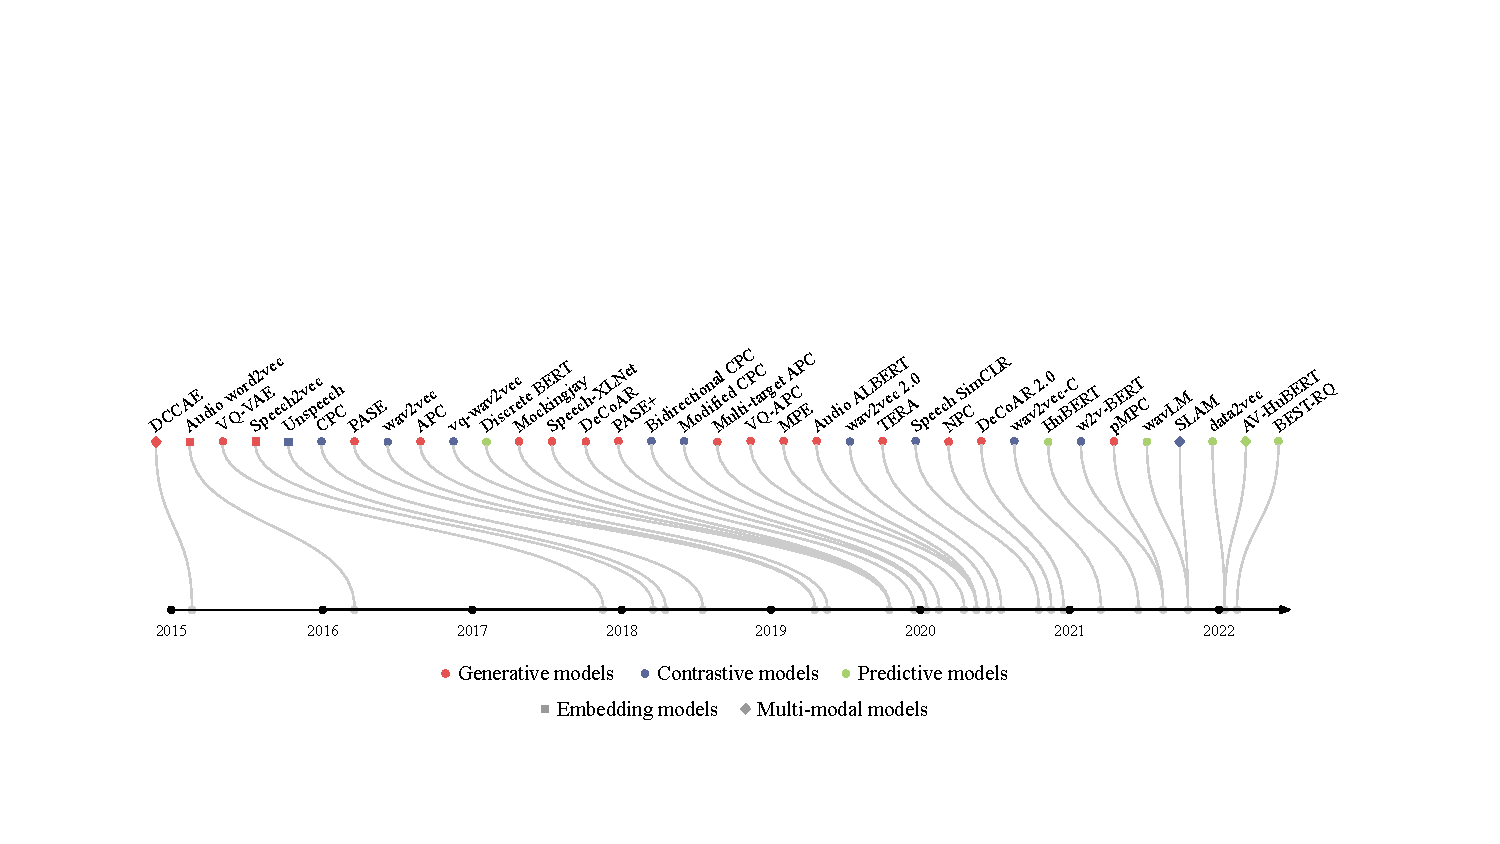
\includegraphics[width=0.98\textwidth]{paper_review/model_timeline.pdf}
   % \includegraphics[width=0.98\textwidth]{paper_review/model_timeline_wo_dccae.pdf}
	 \caption[Selection of self-supervised models for speech.]{A selection of models listed according to first publication date
	 on arXiv or conference submission date when this clearly precedes the
	 former. The models are categorized as generative, contrastive, or predictive.
	 In addition, some models are characterized as embedding models or
	 multi-modal models, although most learn frame-level
	 representations from speech only. Some models use a mixture of generative
	 and contrastive tasks. For instance, PASE and PASE+ use a multi-task setup,
	 but find that generative tasks are the most important for downstream
	 task performance~\parencite{pascual_learning_2019}.}
    \label{fig:timeline}
\end{figure*}


 

\subsection{Generative approaches}
\label{sec:generative}

\subsubsection{Motivation}

In this category, the pretext task is to generate, or reconstruct, the input data based on some limited view. This includes predicting future inputs from past inputs, masked from unmasked, or the original from some other corrupted view.  ``Generative'' as used in this paper hence refers to models that target the original input in their pretext task. Note that this differs from generative models, which learn \ci{distributions that allow} to sample new data.

\subsubsection{Approaches}

\paragraph{Autoencoding} 
Since their introduction in the mid-1990s~\parencite{hinton_autoencoders_1994}, autoencoders (AEs)
have played an essential role in learning distributed latent representations of
sensory data. 
As described above, AEs consist of an encoder and decoder; the pretext task
is to reconstruct the given input. The most common type of AE places an
information bottleneck on the latent representation by simply having fewer
hidden units available than input features. This forces the model to discard
low-level details and disccourages the learning of trivial solutions. Other models add
regularization to the latent space to further improve the quality of the
learned representations.
For instance, denoising autoencoders (DAEs) learn latent representations by
reconstructing from input corrupted by noise~\parencite{vincent_stacked_2010}. 
\edit{The Variational Autoencoder (VAE) is a probabilistic version of the AE which defines the latent representation via a posterior distribution over stochastic latent variables \parencite{kingma_autoencoding_2014,rezende_stochastic_2014}. VAEs have been applied to speech in numerous works \parencite{chung_recurrent_2015, fraccaro_sequential_2016, hsu_learning_2017, hsu_unsupervised_2017, aksan_stcn_2019}}.
The vector-quantized variational autoencoder (VQ-VAE) is another model in this
category~\parencite{oord_neural_2018};
it extends the original VAE~\parencite{kingma_autoencoding_2014} with a novel
parameterization of the posterior distribution for discrete latent
representations. 
\edit{The VQ-VAE has been instrumental in generative speech modelling and recent work on generative spoken language modeling has successfully combined the idea of a discrete latent space with self-supervised learning \parencite{polyak_speech_2021, kharitonov_textfree_2021, nguyen_generative_2022}.}



Specifically, in the VQ-VAE, the continuous representation vector $h_t$ at the output of the encoder is quantized by mapping it to a codebook vector, which is then used as the input to the decoder. This operation is non-differentiable and the \edit{gradients of the loss with respect to the encoder parameters} must be obtained by approximation. In the VQ-VAE this is done using the straight-through estimator~\parencite{bengio_estimating_2013}, i.e., the gradients \edit{with respect to the} encoder output are taken to be equal to those \edit{with respect to the} decoder input \ci{(i.e., the quatization step is ignored)}. Given a learned codebook $A\in\mathbb{R}^{K \times D}$, where $K$ is the codebook size and $D$ is the dimensionality of each codebook vector $a_k$, the quantized representation $q_t$ of $h_t$ is obtained as
\begin{align}
    q_t = a_k, \text{ where } k=\arg\min_j \norm{h_t - a_j}_2 \enspace .
\end{align}
\edit{The decoder $g(\cdot)$ is an autoregressive model that takes $q_{[1,t]}$ as input to generate $x_t$ \parencite{oord_wavenet_2016}}. 
Codebook learning is facilitated by a two-term auxiliary loss similar to
classical vector quantization dictionary 
learning~\parencite{burton_generalization_1983, soong_vector_1985}. 
Gradients for the codebook vectors are given solely by a term that moves
codebook vectors $a_k$ closer to the non-quantized vectors $h_t$. A so-called
\emph{commitment term} is added to ensure that non-quantized vectors do not grow
unboundedly by enforcing the encoder to keep them close to a codebook vector.
This commitment term is optimized only by the encoder. The
total VQ-VAE loss for a single timestep is

\begin{align}
    \mathcal{L}_t = \underset{\text{encoder+decoder}}{\underbrace{\log p(x_t | q_{[1,t]})}}
     + \underset{\text{codebook}}{\underbrace{\text{MSE}\left(\mathrm{sg}\left[h_t\right], A\right)}}
     + \underset{\text{encoder}}{\underbrace{\alpha~\text{MSE}\left(h_t, \mathrm{sg}\left[A\right]\right)}} \enspace ,
    \label{eq: vector quantization losses}
\end{align}%
\noindent where \edit{$\log p(x_t|q_{[1,t]})$ is a reconstruction likelihood term usually using a categorical distribution,} $\mathrm{sg}[x] = x$ is the so-called stop-gradient operator \edit{which acts as the identity function during the forward pass but \ci{is assumed to have}
partial derivatives all equal to zero during the backward pass}, $\alpha$ is a scalar hyperparameter, 
\edit{and we define $\text{MSE}(h_t,A) = \frac{1}{KD} \sum_{k=1}^{K}\sum_{i=1}^{D}\left(h_{t,i} - a_{k,i}\right)^2$. 
The loss for a full sequence is the sum or mean over all $\mathcal{L}_t$.} 

These learned discrete representations have been shown to capture high-level
speech information closely related to phonemes, and are useful for
applications such as speaker conversion~\parencite{chorowski_unsupervised_2019}.
Vector quantization is \edit{not} exclusive to VQ-VAE but has seen
widespread application within SSL for regularization purposes and to define
targets for the pretext task. We will cover these applications below.

\edit{The Gumbel softmax \parencite{jang_categorical_2016} is another frequently used approach for obtaining a discrete representation space, and has also been used for AEs \parencite{eloff_unsupervised_2019}. In addition to the approaches discussed above, several other works on speech representation learning take inspiration from the AE framework \parencite{zeiler_rectified_2013, badino_autoencoder_2014, badino_discovering_2015, kamper_unsupervised_2015, renshaw_comparison_2015, settle_acoustically_2019}.}


\begin{comment}
\paragraph{Regularization}
In the generative-based approaches, some regularization in the encoder $f(\cdot)$ or decoder $g(\cdot)$ is required to encourage the model to utilize global speech information and prevent naive copying input when reconstruction. 
The models below have been enhanced by regularization methods. 
\begin{itemize}
%\item VAE, VQ-VAE
    \item DeCoAR 2.0~\parencite{ling_decoar_2020} presents a deep contextualized acoustic representation learning approach with the addition of a vector quantization (VQ) layer.
    \item In VQ-APC~\parencite{chung_vectorquantized_2020}, a VQ layer is used with the APC objective, which imposes a bottleneck and forces the model to learn better representations.
    \item Two dropout regularization methods, attention dropout and layer dropout, are introduced to TERA~\parencite{luo_dropout_2021}. 
\end{itemize}
\end{comment}

\paragraph{Autoregressive prediction}
\label{par:apc}

Autoregressive predictive coding (APC)~\parencite{chung_unsupervised_2019,
chung_generative_2020} \edit{takes inspiration from the classic Linear Predictive Coding (LPC) approach for speech feature extraction~\parencite{oshaughnessy_linear_1988} and autoregressive language models (LM) for text, where the model learns to predict future information from past}.
\edit{A function} $f(\cdot)$ reads the input sequence $X_{[1,t]}$ and \edit{outputs a representation sequence} $H_{[1,t]}$.
The \edit{auxiliary module} $g(\cdot)$ is a linear projection layer which takes the last vector of $H_{[1,t]}$ as input to \edit{approximate} $x_{t+c}$, where $c \geq 1$. Thus, $c$ indicates how many timesteps the model predicts ahead. The \edit{modules} $f(\cdot)$
and $g(\cdot)$ are jointly learned to minimize {the \ensuremath{L_1} loss between $x_{t+c}$ and its approximation $\hat{x}_{t+c}$}. APC is formulated as 
\begin{align}
    H_{[1,t]} &= f(X_{[1,t]}) , \\
    \hat{x}_{t+c} &= g(h_{t}) \label{eq:c} , \\
    \mathcal{L}_t &= \lVert \hat{x}_{t+c} - x_{t+c} \rVert_1 \enspace .
\end{align}
In text-based autoregressive LMs, $c$ is set to $1$ \edit{to enable autoregressive generation}. However, due to the smoothness of the speech signal, neighboring acoustic features are usually similar. Depending on the downstream task, we are often interested in learning so-called \emph{slow features} that typically span multiple input frames~\parencite{wiskott_slow_2002}. Even the smallest linguistic units of speech---phonemes---span $0.07$~seconds on average in the English TIMIT dataset~\parencite{garofolo_timit_1993},   whereas spectrogram frames $\mathbf{x}_t$ are typically computed at $0.01$ second intervals. Thus, simply predicting the next frame constitutes a trivial pretext task for APC; the original work finds that $c=3$ performs well. 
In \parencite{chung_improved_2020}, the APC objective is extended to multi-target
training. The new objective generates both past and future frames conditioned
on previous context. 
In VQ-APC~\parencite{chung_vectorquantized_2020}, quantization is used with the APC
objective, which imposes an information bottleneck serving as a regularizer.

A drawback of APC is that it encodes information only from previous timesteps
and not the entire input.
DeCoAR~\parencite{ling_deep_2020} combines the bidirectionality of the popular NLP model
ELMo~\parencite{peters_deep_2018} and the reconstruction objective of APC to alleviate
this issue and allow encoding information from the entire input. 
It uses a forward LSTM $f_1(\cdot)$ to encode $X_{[1,t]}$ and a backward LSTM
$f_2(\cdot)$ to encode $X_{[t+k,T]}$, where $k>1$: 
\begin{gather}
    H_{[1,t]} = f_1(X_{[1,t]}), \\
    H^\prime_{[t+k,T]} = f_2(X_{[t+k,T]}), \\
    \hat{X}_{[t+1,t+k-1]} = g(h_t, h^\prime_{t+k}) \enspace .
\end{gather}
The input feature vector used in the downstream tasks is the concatenation of
$h_{t}$ and $h^\prime_{t}$. 


\paragraph{Masked reconstruction}

Masked reconstruction is largely inspired by the masked language model (MLM) task from BERT~\parencite{devlin_bert_2018}. During BERT pre-training, some tokens in the input sentences are masked by randomly replacing them by a learned masking token or another input token. The model learns to reconstruct the masked tokens from the non-masked tokens. Recent work has explored similar pretext tasks \edit{for speech representation learning}. Similar to the DeCoAR model described above, this allows a model to learn contextualized representations that encode information from the entire input. While we here focus on the models that reconstruct the masked input, it is important to note that masking has also been used extensively for contrastive (\cref{contrastive_approaches}) and predictive (\cref{predictive_approaches}) models. 

From a high-level perspective, the training phase of models using masked
reconstruction can be formulated as
\begin{align}
    H &= f(m(X)), \\
    \hat{x}_t &= g(h_{t}), \\
    \mathcal{L}_t &= \lVert \hat{x}_{t} - x_{t} \rVert_1 .
\end{align}
\edit{The exact masking policy defined by $m(\cdot)$ differs from model to model and will be discussed further below.}
The function $f(\cdot)$ is typically a Transformer encoder~\parencite{liu_mockingjay_2020,jiang_improving_2019,liu_masked_2020}, but recurrent neural networks have also been used~\parencite{wang_unsupervised_2020}. \edit{In general, the Transformer encoder architecture has been adopted widely by self-supervised models for speech within all three surveyed categories.} \edit{The function $g(\cdot)$ is usually a linear projection or a multilayer perceptron (MLP)}. Finally, the loss $\mathcal{L}_t$ is commonly computed only for masked timesteps in order to discourage the model from learning an identity mapping.

The masking policies used in NLP can be adapted to speech by considering a speech \edit{segment} equivalent to a token in a sentence; indeed, the masking strategy of BERT has also been used for speech pre-training~\parencite{liu_mockingjay_2020}.
In the standard BERT masking policy, each token is masked independently at random. However, for speech, masking a single \edit{sample or spectrogram frame results in a largely} trivial reconstruction task \edit{since, as discussed in \cref{par:apc}, the smoothness of audio signals may encourage the model to learn to simply interpolate neighboring frames.} Therefore it is common to mask chunks of consecutive frames~\parencite{liu_mockingjay_2020,jiang_further_2021}. 

We can bring the pretext task closer to the NLP equivalent by using a masking policy where the masked regions of the input correspond to linguistic units. Instead of just masking a fixed number of consecutive frames, pMPC~\parencite{yue_phonetically_2021} selects masked speech frames according to the phonetic segmentation in an utterance. \edit{However, in order to obtain this segmentation, some labeled data is of course needed.}

Whereas most studies use masking along the temporal dimension of the input, speech can also be masked along the frequency dimension when spectral input features are used~\parencite{wang_unsupervised_2020,liu_tera_2021}. Frequency masking has been shown to improve representations used for speaker classification~\parencite{liu_tera_2021}. 

Some studies explore alternatives to masking the input directly. In non-autoregressive predictive coding (NPC)~\parencite{liu_nonautoregressive_2020}, time masking is introduced through masked convolution blocks. Taking inspiration from XLNet~\parencite{yang_xlnet_2019}, it has also been suggested that the input be reconstructed from a shuffled version~\parencite{song_speechxlnet_2020} to address the discrepancy between pre-training and fine-tuning of masking-based approaches.

Regularization methods can further improve on masked reconstruction approaches. \edit{DeCoAR 2.0~\parencite{ling_decoar_2020} uses vector quantization}, which is shown to improve the learned representations. Furthermore, two dropout regularization methods---attention dropout and layer dropout---are introduced with the TERA model~\parencite{liu_tera_2021, luo_dropout_2021}. \edit{Both methods are variations on the original dropout method \parencite{srivastava_dropout_2014}.}

\paragraph{More generative approaches}
Other than the autoregressive and masked reconstruction tasks discussed above, various studies have explored the reconstruction of other targets derived from the input. PASE and PASE+~\parencite{pascual_learning_2019,ravanelli_multitask_2020} use multiple targets, including the waveform, log power spectrum, \edit{mel cepstral coefficients (MFCCs)}, and prosody features. Models that learn acoustic embeddings of small speech segments have targeted future and past spectrogram segments~\parencite{chung_speech2vec_2018, tagliasacchi_selfsupervised_2019, tagliasacchi_pretraining_2020}, phase information~\parencite{quitry_learning_2019}, and the temporal gap between two segments~\parencite{tagliasacchi_selfsupervised_2019, tagliasacchi_pretraining_2020}.


\subsubsection{Challenges} 

Although successful NLP models like BERT and GPT are based on generative pretext tasks, the progress have not been translated directly to the speech domain. A speech signal encodes more information than text, such as speaker identity and prosodic features, which makes it harder to generate. However, in order to generate all details of the input, the model must encode all information in the speech signal. Hence, a model that learns to perfectly reconstruct its input may not necessarily have learned to isolate the features of interest \edit{\ci{and will encode} redundant information for a given downstream task.} 

There are many choices involved in designing a generative pretext task. For instance, \edit{masking strategy and the choice of input and target representation (e.g., waveform samples or spectral
features)}. These choices influence what the model learns through the pretext task. However, there is little research on the relationship between task design and the information encoded in the learned representations.

%!TEX root = ../thesis.tex

\begin{table*}[!htb]
    \centering
    \caption{
    A summary of the approaches in the three categories of
    self-supervised learning. 
    Column~(a) lists the names of the models and related references, 
    column~(b) defines the model input, 
    column~(c) defines any corruption of the input or hidden representation, and
    column~(d) defines the target of the pretext task; the pretext task itself
    is described by the overall model category and the main text.
    $X=\{x_1,x_2,...,x_T\}$ is the input sequence in which $x_t$ can be an
    acoustic feature vector (e.g., MFCC, filterbank, or spectrogram features)
    or a waveform sample. 
    $X_{[t_1:t_2]}$ represents $\{x_{t_1},x_{t_1+1},...,x_{t_2}\}$.
    $X_{-[t_1:t_2]}$ represents $X$ in which the segment
    $X_{[t_1:t_2]}=\{x_{t_1},x_{t_1+1},...,x_{t_2}\}$ is masked.
    $x_{t}^{i}$ represents the $i$-th dimension of $x_t$.
    If $x_t$ is a frame in a spectrogram, then the $i$-th dimension corresponds
    to a specific frequency bin.
    $X^{-[f,f+j]}$ refers to a spectrogram $X$ which is masked along the frequency
    axis from the $f$-th to $(f+j)$-th bin. 
    % $X_{-[t:t+k]}^{-[f,f+j]}$ refers to a spectrogram $X$ but masked along both time and frequency dimensions. 
    % $X^*$ is a temporally permuted version of $X$, that is, the $x_t$ are randomly shuffled to form $X^*$. 
    We indicate random temporal permutation of a sequence by indexing it with
    the set $\mathcal{P}_t\triangleq\textsc{permute}([0,t])$, where
    $\textsc{permute}(\cdot)$ returns a permutation of the given list. 
    We indicate data augmentation (e.g., reverberation) by the function
    $\textsc{augment}(\cdot)$. Subscripts indicate different augmentations. 
    % $X^\prime$ is an augmented version of $X$ (e.g., $X$ with reverberation), while $X^{\prime\prime}$ is $X$ adding distortion different from  $X^\prime$.
    $Z$ represents a localized latent representation sequence of $X$. %, and $Z^\prime$ and $Z^{\prime\prime}$ are the latent representation sequences of  $X^\prime$ and $X^{\prime\prime}$, respectively. 
    % $Z$ represents a localized latent representation sequence and $Z^\prime$ is the latent representation sequence of $X^\prime$. 
    $Z^{(l)}$ is $Z$ at the $l$-th layer of the model used to compute it.
    $\bar{H}$ is the contextualized sequence $H$ obtained from an exponential
    moving average (EMA) of the model undergoing training with no masking
    applied.
    $Q$ represents a sequence of quantized learned representations, and $C$ is
    a sequence of discrete cluster IDs.
    For contrastive models, we specify only positive targets.
    }
    % \begin{minipage}{\textwidth}  
\centering
\renewcommand*\arraystretch{1.2}{
\begin{tabular}{l|c|c|c}
    \toprule
    \textbf{Model} (a) & \textbf{Input} (b) & \textbf{Corruption} (c) & \textbf{Target} (d) \\
    \midrule
    \midrule
    \multicolumn{4}{c}{\textsc{Generative models}} \\
    \midrule
    \midrule
    Audio Word2vec~\cite{chung_audio_2016}, VQ-VAE~\cite{oord_neural_2018}     & $X$ &   \textsc{-}    &  $X$  \\ %It has VQ as extra constraint.
    \midrule  
    Speech2Vec~\cite{chung_speech2vec_2018}, Audio2Vec~\cite{tagliasacchi_pre_2020} - skip-gram    & $X_{[t_1,t_2]}$  &     \textsc{-}   &    $X_{[t_0,t_1]}$,$X_{[t_2,t_3]}$     \\
    \midrule 
    Speech2Vec~\cite{chung_speech2vec_2018}, Audio2Vec~\cite{tagliasacchi_pre_2020} - cbow    & $X_{[t_0,t_1]}$,$X_{[t_2,t_3]}$   &     \textsc{-}   &    $X_{[t_1,t_2]}$   \\
    \midrule 
    PASE~\cite{pascual_learning_2019}, PASE+~\cite{ravanelli_multi_2020}\footnote{PASE uses multiple pretext tasks, but the authors find that reconstruction is most important.}       & $X$ &  \textsc{-}   &  Different modalities of $X$  \\
    \midrule 
    APC~\cite{chung_unsupervised_2019,chung_vector-quantized_2020}         & $X_{[1,t]}$   & \textsc{-}              & $x_{t+c},\, c\geq1$    \\ %VQ-APC is the same as APC
    \midrule
    Speech-XLNet \cite{song20d_interspeech}     & \multicolumn{2}{c|}{$X_{\mathcal{P}_{t}}$}   &     $x_{i\sim\mathcal{P}^c_{t}}$  \\ %Lee: Use * to represent the permutation, hope it is not strange.
    \midrule  
    DeCoAR~\cite{ling2020deep}     & $X_{[1,t-1]}, X_{[t+k+1,T]}$ & \textsc{-} & $X_{[t,t+k]}$   \\
    \midrule
    Mockingjay~\cite{liu_mockingjay_2020}, Audio ALBERT~\cite{chi2020audio}, DeCoAR 2.0~\cite{ling2020decoar}   & \multicolumn{2}{c|}{$X_{-[t,t+k]}$}   & $X_{[t,t+k]}$    \\
    \midrule 
    TERA~\cite{liu_tera_2021}, BMR~\cite{wang_unsupervised_2020}  & \multicolumn{2}{c|}{$X_{-[t,t+k]}^{-[f,f+j]}$}       & $X$       \\
    \midrule
    pMPC~\cite{yue_pmpc_2021}      &  \multicolumn{2}{c|}{$X_{-[t,t+k^\prime]}$ ($X_{[t,t+k^\prime]}$ is a phoneme)}       & $X_{[t,t+k^\prime]}$    \\
    \midrule 
    MPE~\cite{liu2020masked} & $X$ &  $Z_{-[t,t+k]}$  & $Z$    \\ %Lee: What is the difference between MPE and NPC??? And I believe it reconstruct the convolutional blocks output (learned target?)
    \midrule
    NPC~\cite{liu21l_interspeech}      & $X$  &   $Z_{-[t,t+k]}$  &    $X$   \\ %Lee: I am not 100% sure it is correct. Please check.
    \midrule
    \midrule
    \multicolumn{4}{c}{\textsc{Contrastive models}} \\
    \midrule
    \midrule
    Unspeech \cite{milde2018unspeech}       &   $X_{[t_1,t_2]}$ &   \textsc{-}   &  $X_{[t_0,t_1]}$,$X_{[t_2,t_3]}$ \\
    \midrule 
    CPC~\cite{oord_representation_2018}, wav2vec \cite{schneider_wav2vec:_2019}, Modified CPC \cite{riviere2020unsupervised}         & $X_{[1,t]}$   &    \textsc{-}           & $z_{t+c},\, c\geq1$   \\ %Modified CPC is the same as CPC
    \midrule 
    Bidirectional CPC \cite{kawakami2020learning}      & $X_{[1,t]}$ or $X_{[t,T]}$ &  \textsc{-}    &    $z_{t+c}$ or $z_{t-c},\, c\geq1$   \\
    \midrule 
    vq-wav2vec \cite{baevski_vq-wav2vec_2020}     &   $X_{[1,t]}$ &   \textsc{-}    &   $q_{t+c},\, c\geq1$   \\ 
    \midrule 
    wav2vec 2.0 \cite{baevski2020wav2vec}, wav2vec-C \cite{sadhu_wav2vec-c_2021}\footnote{wav2vec-C adds reconstruction loss to wav2vec 2.0.}    & $X$             & $Z_{-[t,t+k]}$          & $Q_{[t,t+k]}$ \\
    \midrule 
    w2v-BERT \cite{chung_w2vbert_2021}     &$X$ &    $Z_{-[t,t+k]}$   &     $Q_{[t,t+k]}$ and $C_{[t,t+k]}$     \\
    \midrule
    Speech SimCLR \cite{SpeechSimCLR}\footnote{Speech SimCLR targets the latent representation of an augmented version of $X$ using a differently augmented $X$, and vice-versa.}    & \multicolumn{2}{c|}{$\textsc{augment}_1(X)$ and $\textsc{augment}_2(X)$}     &    $\textsc{augment}_2(Z)$ and $\textsc{augment}_1(Z)$   \\ 
    \midrule
    \midrule 
    \multicolumn{4}{c}{\textsc{Predictive models}} \\
    \midrule
    \midrule
    Discrete BERT~\cite{baevski_vq-wav2vec_2020,baevski_effectiveness_2020} \footnote{Discrete BERT obtains codes $C$ from vq-wav2vec.}      &   \multicolumn{2}{c|}{$C_{-[t,t+k]}$}   & $C_{[t,t+k]}$  \\
    \midrule 
    HuBERT \cite{hsu_hubert_2021}\footnote{HuBERT is trained first using cluster IDs of the MFCCs as target and subsequently clusters IDs of the model representations from the last iteration.}, WavLM \cite{chen_wavlm_2021}\footnote{WavLM simulates noisy/overlapped speech as inputs.}  & $X$             & $Z_{-[t,t+k]}$          & $C_{[t,t+k]}$  \\ 
    \midrule
    data2vec \cite{baevski_data2vec_2022}    & $X$             & $Z_{-[t,t+k]}$          & $\sum_{l}\bar{H}^{(l)}_{[t,t+k]}$  \\ 
    \midrule 
    BEST-RQ \cite{BEST-RQ}\footnote{BEST-RQ obtains codes $C$ by quantizing acoustic features using a random projection quantizer.}     &  \multicolumn{2}{c|}{$X_{-[t,t+k]}$}      &  $C_{[t,t+k]}$   \\ 
    \midrule 
    \bottomrule
\end{tabular}
}
    
% \end{minipage}
\label{table:pretext}
\end{table*}


\begin{comment}
\begin{table*}[ht!]
    \centering
    \caption{
    This table summarizes the approaches of the three categories of self-supervised learning. 
    Column (a) lists the names of the models and related references. 
    Column (b) defines the input to the models. 
    Column (c) defines any corruption of the input or some hidden representation. 
    Column (d) defines the target of the pretext task; the pretext task itself is described by the overall model category and the main text.
    $X=\{x_1,x_2,...,x_T\}$ is the input sequence in which $x_t$ can be an acoustic feature vector (e.g., MFCC, filterbank, or spectrogram features) or a waveform sample. 
    $X_{[t_1:t_2]}$ represents $\{x_{t_1},x_{t_1+1},...,x_{t_2}\}$.
    $X_{-[t_1:t_2]}$ represents $X$ with the segment $X_{[t_1:t_2]}=\{x_{t_1},x_{t_1+1},...,x_{t_2}\}$ masked.
    $x_{t}^{i}$ represents the $i$-th dimension of $x_t$.
    If $x_t$ is a frame in a spectrogram, then the $i$-th dimension corresponds to a specific frequency bin.
    $X^{-[f,f+j]}$ refers to a spectrogram $X$ but masked along the frequency axis from the $f$-th to $f+j$-th bin. 
    % $X_{-[t:t+k]}^{-[f,f+j]}$ refers to a spectrogram $X$ but masked along both time and frequency dimensions. 
    % $X^*$ is a temporally permuted version of $X$, that is, the $x_t$ are randomly shuffled to form $X^*$. 
    We indicate random temporal permutation of a sequence by indexing it with the set $\mathcal{P}_t\triangleq\textsc{permute}([0,t])$ where $\textsc{permute}(\cdot)$ returns a permutation of the given list. 
    We indicate data augmentation (e.g. reverberation) by the function $\textsc{augment}(\cdot)$. Subscripts indicate different augmentations. 
    % $X^\prime$ is an augmented version of $X$ (e.g., $X$ with reverberation), while $X^{\prime\prime}$ is $X$ adding distortion different from  $X^\prime$.
    $Z$ represents a localized latent representation sequence of $X$. %, and $Z^\prime$ and $Z^{\prime\prime}$ are the latent representation sequences of  $X^\prime$ and $X^{\prime\prime}$, respectively. 
    % $Z$ represents a localized latent representation sequence and $Z^\prime$ is the latent representation sequence of $X^\prime$. 
    $Z^{(l)}$ is $Z$ at the $l$-th layer of the model used to compute it.
    $\bar{H}$ is the contextualized sequence $H$ obtained from an exponential moving average (EMA) of the model undergoing training with no masking applied.
    $Q$ represents a sequence of quantized learned representations, and $C$ is a sequence of discrete cluster IDs.
    For contrastive models, we specify only positive targets.
    }
    \begin{minipage}{\textwidth}  
    \centering
    \renewcommand*\arraystretch{1.1}{
    \begin{tabular}{l|c|c|c}
    \toprule
    \textbf{Model} (a) & \textbf{Input} (b) & \textbf{Corruption} (c) & \textbf{Target} (d) \\
    \midrule
    \midrule
    \multicolumn{4}{c}{\textsc{Generative models}} \\
    \midrule
    \midrule
    Audio Word2vec~\cite{chung_audio_2016}, VQ-VAE \cite{oord_neural_2018}     & $X$ &   \textsc{-}    &  $X$  \\ %It has VQ as extra constraint.
    \midrule  
    Speech2Vec~\cite{chung_speech2vec_2018}, Audio2Vec~\cite{tagliasacchi_pre_2020} - skip-gram    & $X_{[t_1,t_2]}$  &     \textsc{-}   &    $X_{[t_0,t_1]}$,$X_{[t_2,t_3]}$     \\
    \midrule 
   Speech2Vec~\cite{chung_speech2vec_2018}, Audio2Vec~\cite{tagliasacchi_pre_2020} - cbow    & $X_{[t_0,t_1]}$,$X_{[t_2,t_3]}$   &     \textsc{-}   &    $X_{[t_1,t_2]}$   \\
    \midrule 
     PASE~\cite{pascual_learning_2019}, PASE+~\cite{ravanelli_multi_2020}\footnote{PASE uses multiple pretext tasks, but the authors find that reconstruction is most important.}       & $X$ &  \textsc{-}   &  Different modalities of $X$  \\
    \midrule 
    APC~\cite{chung_unsupervised_2019,chung_vector-quantized_2020}         & $X_{[1,t]}$   & \textsc{-}              & $x_{t+c},\, c\geq1$    \\ %VQ-APC is the same as APC
    \midrule
    Speech-XLNet \cite{song20d_interspeech}     & \multicolumn{2}{c|}{$X_{\mathcal{P}_{t}}$}   &     $x_{i\sim\mathcal{P}^c_{t}}$  \\ %Lee: Use * to represent the permutation, hope it is not strange.
    \midrule  
    DeCoAR~\cite{ling2020deep}     & $X_{[1,t-1]}, X_{[t+k+1,T]}$ & \textsc{-} & $X_{[t,t+k]}$   \\
    \midrule
    Mockingjay~\cite{liu_mockingjay_2020}, Audio ALBERT~\cite{chi2020audio}, DeCoAR 2.0~\cite{ling2020decoar}   & \multicolumn{2}{c|}{$X_{-[t,t+k]}$}   & $X_{[t,t+k]}$    \\
    \midrule 
    TERA~\cite{liu_tera_2021}, BMR~\cite{wang_unsupervised_2020}  & \multicolumn{2}{c|}{$X_{-[t,t+k]}^{-[f,f+j]}$}       & $X$       \\
    \midrule
    pMPC~\cite{yue_pmpc_2021}      &  \multicolumn{2}{c|}{$X_{-[t,t+k^\prime]}$ ($X_{[t,t+k^\prime]}$ is a phoneme)}       & $X_{[t,t+k^\prime]}$    \\
    \midrule 
    MPE~\cite{liu2020masked} & $X$ &  $Z_{-[t,t+k]}$  & $Z$    \\ %Lee: What is the difference between MPE and NPC??? And I believe it reconstruct the convolutional blocks output (learned target?)
    \midrule
    NPC~\cite{liu21l_interspeech}      & $X$  &   $Z_{-[t,t+k]}$  &    $X$   \\ %Lee: I am not 100% sure it is correct. Please check.
    \midrule
    \midrule
    \multicolumn{4}{c}{\textsc{Contrastive models}} \\
    \midrule
    \midrule
    Unspeech \cite{milde2018unspeech}       &   $X_{[t_1,t_2]}$ &   \textsc{-}   &  $X_{[t_0,t_1]}$,$X_{[t_2,t_3]}$ \\
    \midrule 
    CPC~\cite{oord_representation_2018}, wav2vec \cite{schneider_wav2vec:_2019}, Modified CPC \cite{riviere2020unsupervised}         & $X_{[1,t]}$   &    \textsc{-}           & $z_{t+c},\, c\geq1$   \\ %Modified CPC is the same as CPC
        \midrule 
    Bidirectional CPC \cite{kawakami2020learning}      & $X_{[1,t]}$ or $X_{[t,T]}$ &  \textsc{-}    &    $z_{t+c}$ or $z_{t-c},\, c\geq1$   \\
    \midrule 
    vq-wav2vec \cite{baevski_vq-wav2vec_2020}     &   $X_{[1,t]}$ &   \textsc{-}    &   $q_{t+c},\, c\geq1$   \\ 
    \midrule 
    wav2vec 2.0 \cite{baevski2020wav2vec}, wav2vec-C \cite{sadhu_wav2vec-c_2021}\footnote{wav2vec-C adds the reconstruction loss to wav2vec 2.0.}    & $X$             & $Z_{-[t,t+k]}$          & $Q_{[t,t+k]}$ \\
    \midrule 
    w2v-BERT \cite{chung_w2vbert_2021}     &$X$ &    $Z_{-[t,t+k]}$   &     $Q_{[t,t+k]}$ and $C_{[t,t+k]}$     \\
    \midrule
    Speech SimCLR \cite{SpeechSimCLR}\footnote{Speech SimCLR targets the latent representation of an augmented version of $X$ using a differently augmented $X$, and vice-versa.}    & \multicolumn{2}{c|}{$\textsc{augment}_1(X)$ and $\textsc{augment}_2(X)$}     &    $\textsc{augment}_2(Z)$ and $\textsc{augment}_1(Z)$   \\ 
   \midrule
   \midrule 
    \multicolumn{4}{c}{\textsc{Predictive models}} \\
    \midrule
    \midrule
    Discrete BERT~\cite{baevski_vq-wav2vec_2020,baevski_effectiveness_2020} \footnote{Discrete BERT obtains codes $C$ from vq-wav2vec.}      &   \multicolumn{2}{c|}{$C_{-[t,t+k]}$}   & $C_{[t,t+k]}$  \\
    \midrule 
    HuBERT \cite{hsu_hubert_2021}\footnote{HuBERT is trained first using cluster IDs of MFCCs as target and subsequently cluster IDs of model representations from the last iteration.}, WavLM \cite{chen_wavlm_2021}\footnote{WavLM simulates noisy/overlapped speech as inputs.}  & $X$             & $Z_{-[t,t+k]}$          & $C_{[t,t+k]}$  \\ 
    \midrule
    data2vec \cite{baevski_data2vec_2022}    & $X$             & $Z_{-[t,t+k]}$          & $\sum_{l}\bar{H}^{(l)}_{[t,t+k]}$  \\ 
        \midrule 
BEST-RQ \cite{BEST-RQ}\footnote{BEST-RQ obtains codes $C$ by quantizing acoustic features using a random projection quantizer.}     &  \multicolumn{2}{c|}{$X_{-[t,t+k]}$}      &  $C_{[t,t+k]}$   \\ 
        \midrule 
    \bottomrule
    \end{tabular}
    }
    
    \end{minipage}
    \label{table:pretext}
\end{table*}
\end{comment}

\begin{comment}
\begin{table*}[h!]
\centering

\setlength{\tabcolsep}{3pt}
\caption{
This table summarizes the generative approaches. 
Column (a) is the name of the models (if any) and their reference.
Column (b) is the corrupted speech signals for encoder input.
Column (c) is the target output of decoder.
Column (d) is regularization methods used if any.
Column (e) are the models using the same pretext in NLP or CV.
$S$ is a sequence of waveform samples, and $s_t$ is a single waveform sample.
$S^*$ is the degradation of $S$ with reverberation or additive noises. 
$S$ can be represented by a sequence of acoustic feature, $X=\{x_1,x_2,...,x_T\}$, in which $x_t$ is an acoustic feature vector like MFCC, fbank, spectrogram, etc. 
$X^*$ is the permuted version of $X$. That is, the frames in $X$ are randomly shuffled to form $X^*$. 
$X_{[t_1:t_2]}$ represents $\{x_{t_1},x_{t_1+1},...,x_{t_2}\}$.
$X_{-[t_1:t_2]}$ represents the segment $\{x_{t_1},x_{t_1+1},...,x_{t_2}\}$ in $X$ is masked, that is, the frames in the region is replaced by zero vectors or random sampled vectors.
$x_{t}^{i}$ represents the $i$-th dimension of frame $x_t$.
If $x_t$ is a frame in a spectrogram, then the $i$-th dimension corresponds to a specific frequency bin.
$X^{-[f_1,f_2]}$ means that for all the frames $x$ in $X$, their $f_1$-th to $f_2$-th dimensions are all masked. 
$X_{-[t_1:t_2]}^{-[f_1,f_2]}$ means $X$ are masked in two directions. 
}
\label{table:generative}
  {\renewcommand*\arraystretch{1.2}
\begin{tabular}{|l|l|l|l|l|}
\hline
(a) Model & (b) Corrupted Input & (c) Target Output & (d) Regularization &   (e) Counterparts \\ 
\hline \hline 

APC~\cite{chung_unsupervised_2019, chung_generative_2020,chung2020improved} & $X_{[1,t-1]}$  & $x_{t+c},c\geq0$ & VQ~\cite{chung_vector-quantized_2020} &  GPT~\cite{alex2018GPT,radford_language_2019,brown2020gpt3} \\ \hline

%$X_{[1,t-1]}$  & $x_{t+c},c\geq0$ & VQ & VQ-APC~\cite{chung_vector-quantized_2020} & -  \\

DeCoAR~\cite{ling2020deep} & $X_{[1,t-1]}$, $X_{[t+k+1,T]}$ &  $X_{[t,t+k]}$ & VQ~\cite{ling2020deep} &  ELMo~\cite{Matthew2018ELMO} \\
\hline

\tabincell{l}{ Mockingjay~\cite{liu_mockingjay_2020} \\ MPC~\cite{jiang2019improving,jiang_further_2021} \\ AALBERT~\cite{chi2021aalbert} \\
DeCoAR 2.0~\cite{ling2020decoar} } &
$X_{-[t,t+k]}$ & $X_{[t,t+k]}$ & VQ~\cite{ling2020decoar} &  \tabincell{l}{BERT ~\cite{devlin_bert:_2018}\\RoBERTa~\cite{liu_roberta_2019}} \\ \hline

pMPC~\cite{yue_pmpc_2021}   &
\tabincell{l}{$X_{-[t,t+k^\prime]}$\\($X_{[t,t+k^\prime]}$: phoneme-level segment)} & $X_{[t,t+k^\prime]}$ & - &  SpanBert~\cite{joshi-etal-2020-spanbert} \\ \hline

speech-XLNet~\cite{song20d_interspeech} &
$X^*_{[1:t-1]}$ & $x^*_t$ & - &  XLNet~\cite{Yang2019LNet}   \\ \hline

\tabincell{l}{NPC~\cite{liu21l_interspeech}\\MPE~\cite{liu2020masked}} &
\tabincell{l}{$X_{-[t,t+k]}$\\(mask on hidden layer)} & $X_{[t,t+k]}$ & - &   - \\ \hline

\tabincell{l}{BMR~\cite{wang_unsupervised_2020}\\TERA~\cite{liu_tera_2021}} &
$X_{-[t_1:t_2]}^{-[f_1,f_2]}$ & $X$ & dropout~\cite{luo_drop_2021} &  -  \\ \hline

\cite{chorowski_unsupervised_2019} &
$S$ & $S$ & \tabincell{l}{VQ-VAE~\cite{chorowski_unsupervised_2019}\\time-jitter regularizer~\cite{chorowski_unsupervised_2019}} & 
\tabincell{l}{\cite{van2017neural,razavi_generating_2019} \\ (just name a few)} \\ \hline

\cite{tagliasacchi_self_2019, tagliasacchi_pre_2020} & 
$X_{[t-k,t-1]},X_{[t+k+1,t+2k]}$ & $X_{[t,t+k]}$  & - & CBoW~\cite{mikolov2013efficient}  \\ \hline

\cite{tagliasacchi_self_2019, tagliasacchi_pre_2020} &
$X_{[t,t+k]}$ & $X_{[t-k,t-1]},X_{[t+k+1,t+2k]}$ & - &  Skipgram~\cite{mikolov2013efficient} \\ \hline

\cite{quitry2019learning}  &
Magnitude of $X$ & Phase of $X$ & - &  - \\ \hline

TemporalGap~\cite{tagliasacchi_self_2019, tagliasacchi_pre_2020} &
$X_{[t_1,t_1+k]}$, $X_{[t_2,t_2+k]}$ & $|t_1 - t_2|$ & - &  -  \\ \hline

\cite{Carr2021Ranking} &
$X^*$ & correct order & - &  Jigsaw~\cite{noroozi2016unsupervised} \\ 
\hline 

PASE~\cite{pascual_learning_2019} &
$S$ & $X$: LPS, MFCC, Prosody & - &  -  \\ \hline

PASE+~\cite{ravanelli_multi_2020} & 
$S^*$ & \tabincell{l}{$X$: LPS, MFCC, Prosody, \\ fbank, gammatone} & -  &  -  \\ \hline
\end{tabular}
}
\end{table*}
\end{comment}





\subsection{Contrastive approaches}
\label{contrastive_approaches}
\subsubsection{Motivation}
As discussed above, speech contains many entangled features. Thus, \edit{learning to reconstruct the raw speech signal} might not be the best way to discover contextualized latent factors of variations. 
Contrastive models learn representations by distinguishing a target sample (positive) from distractor samples (negatives) given an \emph{anchor representation}. \edit{The pretext task is to maximize latent space similarity between the anchor and positive samples while minimizing the similarity between the anchor and negative samples}. This approach has been used extensively in the general \edit{ML} community \parencite{schultz_learning_2003}.

\subsubsection{Approaches}
\paragraph{CPC}
\label{par:cpc}
Contrastive Predictive Coding (CPC)~\parencite{oord_representation_2018} is a prominent example of a contrastive model. 
\edit{CPC uses a convolutional module $f_1(\cdot)$ to produce localized representations $z_t$ with a recurrent module $f_2(\cdot)$ on top that outputs a contextualized representation $h_t$. An anchor representation $\hat{z}_{t,k}$ is obtained via a linear projection $g_k(\cdot)$ of $h_t$. The positives and negatives are sampled from the localized representation $Z$.
Hence, at a single timestep $t$, CPC forms multiple anchor representations $\hat{z}_{t,k}$ for $k\in\{1,\dots,K\}$ and associates with each one a single positive sample at the corresponding timestep, $z_{t+k}$, $k$ steps in the future:
\begin{align}
    z_t &= f_{1}(X_{[t-u,t+u]}) \label{eq: cpc local representation} \enspace ,\\
    H_{[1,t]} &= f_{2}(Z_{[1,t]}) \enspace , \\
    \hat{z}_{t,k} &= g_k(h_{t}) \enspace.
\end{align}
%
\noindent Each $z_{t}$ only encodes information from a limited receptive field, while $f_2(\cdot)$ is limited to condition each $h_t$ on previous timesteps $Z_{[1,t]}$. \ci{Without these restrictions}, the model could collapse to a trivial solution. $g_k$ is a unique transformation per \ci{offset} $k$ (e.g., a linear projection).
The loss function measures the similarity between the anchor representation $\hat{z}_{t,k}$ and the positive $z_{t+k}$ normalized by the total similarity to the positive and negatives.}
The approach is similar to previous work on Noise-Contrastive Estimation (NCE)~\parencite{gutmann_noisecontrastive_2010}. \edit{Minimizing} the loss corresponds to maximizing a lower bound on the mutual information between $h_t$ and $z_{t+k}$ (and in turn $x_{t+k-u:t+k+u}$) and is hence called InfoNCE:
\begin{align}
    \mathcal{L}_{t,k} &= - \log \left(\frac{\exp(\hat{z}_{t,k}^{\text{\tiny T}}z_{t+k})}{\sum_{\ci{i \in \mathcal{I}}} \exp(\hat{z}_{t,k}^{\text{\tiny T}}z_{i})} \right)\enspace .
    \label{eq: cpc loss}
\end{align}
\noindent \edit{Here, $\mathcal{I}$ \ci{is a random subset of $N$} indices  which includes the target index $t+k$ and $N-1$ negative samples drawn from a proposal distribution, e.g., a uniform distribution over $\{1,\dots,T\}$. Including the target index in $\mathcal{I}$ ensures that the loss is a proper categorical cross-entropy and that minimizing it has the previously stated relation to mutual information maximization}. This corresponds to sampling negatives from the same sequence and has been \edit{shown} to give good performance for phoneme classification~\parencite{oord_representation_2018}. The loss is indexed by $k$ to show that CPC targets multiple offsets using different projection layers $g_k(\cdot)$. The authors find \edit{$K=12$} to work well for phoneme classification.

The wav2vec model \parencite{schneider_wav2vec_2019} extends the CPC approach \edit{and uses fully convolutional parameterizations for the modules $f_1(\cdot)$ and $f_2(\cdot)$ with receptive fields of \SI{30}{ms} and \SI{210}{ms}, respectively. While the CPC loss solves a 1-of-$N$ classification task per $(t,k)$, either assigning the anchor to the positive class or (wrongly) to one of the $N-1$ negative classes, the wav2vec loss considers a sequence of $N$ independent binary classifications. That is, the anchor is compared independently to the positive and each negative, and the loss is computed as a sum of the associated log-probabilities,
\begin{align}
    \mathcal{L}_{t,k} &= - \log(\sigma(\hat{z}_{t,k}^{\text{\tiny T}}z_{t+k})) + \sum_{i \in \mathcal{I}} \log(1 - \sigma(\hat{z}_{t,k}^{\text{\tiny T}}z_{i})) \enspace .
    \label{eq: wav2vec loss}
\end{align}
\noindent Here, $\sigma(x)=1/(1+\exp(-x))$ is the sigmoid function, $\sigma(\hat{z}_{t,k}^{\text{\tiny T}}z_{t+k})$ is the probability of the anchor being the positive sample and $\sigma(\hat{z}_{t,k}^{\text{\tiny T}}z_{i})$ is the probability of the anchor being the negative sample. Evidently and contrary to CPC, $\mathcal{I}$ must not include the target index $t+k$ as this would cancel out the positive term.}

\paragraph{wav2vec 2.0} 
\edit{The wav2vec 2.0 model combines contrastive learning with masking}. As the CPC model, it uses the InfoNCE loss \parencite{oord_representation_2018} to maximize the similarity between a contextualized representation and a localized representation. \edit{However, instead of using the $z_t$ directly as positive and negatives, it uses a quantization module $g(\cdot)$ to obtain a discrete representation. This has the practical implication that one can avoid sampling negatives from the same category as the positive}. \edit{The model} takes as input a waveform and uses a convolutional module \edit{$f_1(\cdot)$} followed by a \edit{Transformer encoder} \edit{$f_2(\cdot)$}. Masking is applied to the output of the convolutional module: 
\begin{align}
    z_t &= f_1(X_{[t-u,t+u]}) \label{w2v2 f_v} \enspace , \\
    H &= f_2(m(Z)) \label{w2v2 f_c} \enspace , \\
    q_t &= g(z_t) \enspace . \label{w2v2 qtz}
\end{align}
\noindent
The quantization module $g(\cdot)$ uses a Gumbel softmax~\parencite{jang_categorical_2016} with a straight-through estimator. Since the quality of the learned representations is contingent on the quality of the quantization, wav2vec 2.0 combines two techniques to learn high-quality codebooks. First, wav2vec 2.0 concatenates quantized representations from multiple codebooks at each timestep, so-called Product Quantization (PQ)~\parencite{jegou_product_2011}. Also, the \edit{primary} training loss \edit{described below} is augmented with an auxiliary term designed to encourage equal use of all codebook entries. 

In wav2vec 2.0, anchors are taken to be $h_t$ at masked timesteps only, the positive sample is chosen as the quantized vector, $q_t$, at the same timestep, and negatives are sampled from other masked timesteps. The loss is
%
\begin{align}
    \mathcal{L}_t &= - \log \left(\frac{\exp(S_{\text{c}}(h_{t}, q_{t}))}{\sum_{i \in \mathcal{I}} \exp(S_{\text{c}}(h_{t}, q_{i}))} \right) \enspace , \label{w2v2 loss}
\end{align}
%
\noindent where $S_{\text{c}}(\cdot)$ is the cosine similarity and $\mathcal{I}$ contains the target index $t$ and negative indices sampled from other masked timesteps.

The wav2vec 2.0 approach was the first to reach single-digit \edit{word error rate (WER) on LibriSpeech using only the low-resource Libri-light subsets for fine-tuning a pre-trained model (see \cref{sec:datasets}). It has subsequently} inspired many follow-up studies. The wav2vec-C~\parencite{sadhu_wav2vecc_2021} approach extends wav2vec 2.0 with a consistency term in the loss that aims to reconstruct the input features from the learned quantized representations, similar to VQ-VAE~\parencite{razavi_generating_2019}.

\subsubsection{Challenges}
Although representations learned using contrastive approaches have proved effective across a wide range of downstream applications, they face many challenges when applied to speech data. 
One challenging aspect is that the strategy used to define positive and negative samples can also indirectly impose invariances on the learned representations. For example, sampling negatives exclusively from the same utterance as the positive biases the features towards speaker invariance, which may or may not be desired for downstream applications. 
Another standing challenge is that since speech input does not have explicit segmentation of acoustic units, the negative and positive samples do not represent a whole unit of language but rather partial or multiple units, depending on the span covered by each sample. 
Finally, since speech input is smooth and lacks natural segmentation, it can be difficult to define a contrastive sampling strategy that is guaranteed to provide samples that always relate to the anchor as truly positives and negatives in a sound way.

\subsection{Predictive approaches}
\label{predictive_approaches}
\subsubsection{Motivation}
\edit{Similar to the contrastive approaches discussed above, predictive approaches are defined by using a learned target for the pretext task. However, unlike the contrastive approaches, they do not employ a contrastive loss and instead use a loss function such as squared error and cross-entropy. 
Whereas a contrastive loss discourages the model from learning a trivial solution by the use of negative samples, this must be circumvented differently for predictive methods.
For this reason, predictive methods compute the targets outside the model's computational graph; usually with a completely separate model. Thus, the predictive setup is somewhat akin to teacher-student training. The first predictive approaches were motivated by the success of BERT-like methods in NLP \parencite{devlin_bert_2018} as well as the DeepCluster method in CV \parencite{caron_deep_2018}.}

\subsubsection{Approaches}

\paragraph{Discrete BERT} \edit{Applying BERT-type training directly to speech input is not possible due to its continuous nature}. The Discrete BERT approach~\parencite{baevski_effectiveness_2020} uses a pre-trained vq-wav2vec model to derive a discrete vocabulary \parencite{baevski_vqwav2vec_2020}. The vq-wav2vec model is similar to wav2vec mentioned in \cref{par:cpc} but uses quantization to learn discrete representations. 
\edit{Specifically, discrete units $c_t$ are first extracted with the vq-wav2vec model $f_1(\cdot)$ and then used as inputs \emph{and} targets in a standard BERT model $f_2(\cdot)$ with a softmax normalized output layer $g(\cdot)$, 
\begin{align}
    c_t &= f_1(X_{[t-u,t+u]}) \enspace , \\
    H &= f_2(m(C)) \enspace , \\
    \hat{c}_t &= g(h_t) \enspace .
\end{align}
Similar to BERT, the model can then be trained with a categorical cross-entropy loss,
\begin{align}
    \mathcal{L} &= \sum_{t\in \mathcal{M}} - \log p(c_t \mid X) \enspace ,
\end{align}
\noindent where $\mathcal{M}$ is the set of all masked timesteps. During training, only the BERT model's parameters are updated, while the vq-wav2vec model parameters are frozen.} 
Discrete BERT was the first model to demonstrate the effectiveness of self-supervised speech representation learning by achieving a WER of 25\% on the standard test-other subset using a 10-minute fine-tuning set, \edit{setting the direction for many approaches to follow}.

\paragraph{HuBERT} Rather than relying on an advanced representation learning model for discretizing continuous inputs, as Discrete BERT, the Hidden Unit BERT (HuBERT) approach \parencite{hsu_hubert_2021} \edit{uses quantized MFCC features as targets learned with classic $k$-means. Thus, to compute the targets, the $k$-means model $g_1(\cdot)$ assigns a cluster center to each timestep.  
Different from Discrete BERT, HuBERT takes the raw waveform as input, rather than discrete units. This helps to prevent loss of any relevant information due to input quantization.
HuBERT uses an architecture similar to that of wav2vec 2.0, with a convolutional module $f_1(\cdot)$ and a Transformer encoder $f_2(\cdot)$, as well as a softmax normalized output layer $g_2(\cdot)$:
\begin{align}
    c_t &= g_1(X_{[t-w,t+w]}) \enspace , \\
    z_t &= f_1(X_{[t-u,t+u]}) \enspace , \\
    H &= f_2(m(Z)) \enspace , \\
    \hat{c}_t &= g_2(h_t) \enspace ,
\end{align}
\noindent where $w$ defines the window size used to compute the MFCCs. 
The categorical cross-entropy loss is} computed on both masked, $\mathcal{L}_m$, and unmasked, $\mathcal{L}_u$, timesteps:  
\begin{align}
    \mathcal{L}_m &= \sum_{t\in \mathcal{M}} - \log p(c_t \mid X) \enspace , \\
    \mathcal{L} &= \beta
    \mathcal{L}_m + (1 - \beta) \mathcal{L}_u \enspace .
\end{align}
%
\noindent Again, $\mathcal{M}$ is the set of all masked timesteps, $\beta$ is a scalar hyperparameter and $\mathcal{L}_u$ is computed as $\mathcal{L}_m$ but summing over $t\notin \mathcal{M}$.

Intuitively, the HuBERT model is forced to learn both \edit{an acoustic and a language model. 
First, the model needs to learn a meaningful continuous latent representation for unmasked timesteps which are mapped to discrete units, similar to a classical frame-based acoustic modeling problem. Second, similar to other masked pre-training approaches, the model needs to capture long-range temporal dependencies to make correct predictions for masked timesteps}.

One crucial insight motivating this work is the importance of consistency of the targets which enables the model to focus on modeling the sequential structure of the input. \edit{Importantly though, for HuBERT, pre-training is a two-step procedure. The first iteration is described above.
Once completed, a second iteration of pre-training follows. Here, representations from a hidden layer of the model from the first iteration are clustered with $k$-means to obtain new targets $c_t$.}

\edit{For HuBERT, only two iterations are needed to match or outperform the previous state-of-the-art results for low-resource speech recognition. And combining the HuBERT approach with the wav2vec 2.0 approach, the w2v-BERT model has managed to improve results even further~\parencite{chung_w2vbert_2021}.}


\paragraph{WavLM}

\edit{WavLM emphasizes spoken content modeling and speaker identity preservation~\parencite{chen_wavlm_2021}. It is largely identical to HuBERT, but introduces two useful extensions.}

\edit{First, it extends the Transformer self-attention mechanism with a so-called \emph{gated relative position bias}. The bias is added prior to the softmax normalization of the attention weights. For the attention weight at $i,j$, the bias is computed based on the input to the Transformer layer at the current time step $i$ and also incorporates a relative positional embedding for $i-j$. The authors find that this extension improves performance on phoneme and speech recognition tasks.}

\edit{Second, it uses an utterance mixing strategy where signals from different speakers are combined to augment the training data.} \edit{Specifically, random subsequences from other examples in the same batch are scaled and added to each input example.
Only the targets corresponding to the original example are predicted during pre-training. Thus, the model learns to filter out the added overlapping speech.}

Most SSL methods are trained on data \edit{where each example only contains speech from a single person}; therefore, they can perform subpar on multispeaker tasks like speaker separation and diarization. 

The WavLM model achieved substantial improvements on the speech separation, speaker verification and speaker diarization tasks in the SUPERB benchmark, while also performing well on many other tasks compared to HuBERT and wav2vec 2.0.

\paragraph{data2vec} \edit{Motivated by the success of using an exponential moving average (EMA) teacher for self-supervised visual representations~\parencite{grill_bootstrap_2020, caron_emerging_2021}, the data2vec model~\parencite{baevski_data2vec_2022} computes targets $Y$ using an EMA of its own parameters. The targets are constructed by averaging hidden representations of the top $k$ layers of the EMA teacher network applied to unmasked inputs. Here, we denote this jointly as $\bar{f}_2(\cdot)$.

The data2vec model was proposed for different data modalities, but for audio it uses an architecture similar to wav2vec 2.0 and HuBERT with a convolutional module $f_1(\cdot)$, a Transformer $f_2(\cdot)$ and masking applied to the Transformer input.
\begin{align}
    z_t &= f_1(X_{[t-u,t+u]}) \enspace , \\
    H &= f_2(m(Z)) \enspace , \\
    Y &= \bar{f}_2(Z) \enspace .
\end{align}
The teacher network $\bar{f}_2(\cdot)$ is a copy of the Transformer of the student network but with the parameters at training step $i$, $\theta_{\text{teacher},i}$, given by an EMA of the student parameters over all previous training steps.
\begin{equation}
    \theta_{\text{teacher},i} = \begin{cases}
        \theta_{\text{student},0} & i = 0 \\
        \gamma\theta_{\text{student},i} + (1-\gamma)\theta_{\text{teacher},i-1} & i > 0 
    \end{cases} \enspace ,
\end{equation}
\noindent where $\theta_{\text{student},i}$ are the parameters of the student network at training step $i$, updated via gradient descent, and $\gamma$ is the EMA decay rate. 

The data2vec model uses a regression loss between target and prediction. Specifically, to reduce sensitivity to outliers and prevent exploding gradients, it uses the smoothed \ensuremath{L_1} loss \parencite{girshick_fast_2015},
\begin{equation}
\mathcal{L}_t =
    \begin{cases}
      \frac{1}{2}(y_t - h_t)^2 / \eta\text{,} & |y_t - h_t| \leq \eta\\
      |y_t - h_t| - \frac{1}{2}\eta\text{,} & \text{otherwise}
    \end{cases} \enspace ,
\end{equation}
\noindent where the hyperparameter $\eta$ controls the transition from a squared loss to an \ensuremath{L_1} loss.}

\edit{The data2vec approach was shown to work well for representation learning with either speech, images or text data.} It is the first approach to achieve competitive results when trained on \edit{any} one of the three modalities. 

\subsubsection{Challenges}
The iterative nature of pre-training for the HuBERT and wavLM could present a practical inconvenience when working with large volumes of data. Another challenge for these models centers around the quality of the initial vocabulary generated from MFCC features. 
The data2vec approach improves over other predictive models \edit{by allowing the targets to improve continuously via the EMA teacher network}; however, \edit{student-teacher approaches inflate the existing computational challenges of very large models and may necessitate the use of methods that decrease instantaneous memory utilization such as mixed precision training, model parallelism and model sharding \parencite{paszke_automatic_2017}.}

\subsection{Learning from multi-modal data}
\subsubsection{Motivation}
Multiple modalities are useful in many settings, where each modality provides information that is complementary to other modalities.  Multi-modal work includes supervised settings, such as audio-visual ASR~\parencite{petajan_automatic_1984,potamianos_recent_2003} and person identification~\parencite{aleksic_audiovisual_2006} which have been studied for decades.  In this section, we focus only on unsupervised representation learning from multi-modal data.

One of the motivations for learning from multiple modalities is that it can reduce the effect of noise, since noise in different modalities is likely to be largely independent or uncorrelated.  In addition, learning from speech data with accompanying signals such as images or video can help learn representations that encode more semantic information. Such ``grounding" signals can contain supplementary information that can be used by models to infer the content of the speech. Human language learning provides a proof of concept for this, as it is believed that infants benefit from the visual modality when learning language~\parencite{legerstee_infants_1990}. Early computational models of multi-modal language learning were motivated by (and tried to emulate) human learning of language in the context of the visual surroundings~\parencite{roy_learning_1999}.

\subsubsection{Approaches}
We define two broad classes of approaches in this area. Specifically, depending on what type of multi-modal data is involved we refer to ``intrinsic" or ``extrinsic" modalities.

\edit{\textit{Intrinsic modalities} are} 
modalities produced directly by the speech source.  Examples of intrinsic modalities (besides the speech audio) include images or video of the speaker's face~\parencite{lee_avicar_2004,chung_lip_2016}, lip-movement~\parencite{shi_learning_2022}, articulatory flesh point measurements~\parencite{westbury_xray_1990,wrench_new_2001}, or simultaneous \edit{magnetic resonance imaging (MRI)} scans~\parencite{narayanan_multimodal_2011}.  Typically, learning from multiple intrinsic modalities is done so as to improve robustness to noise, since acoustic noise is likely to be uncorrelated with the other \edit{modality(ies)}.  This type of representation learning is often referred to as ``multi-view learning" because the multiple intrinsic modalities can be seen as multiple views of the same content. Some typical approaches in this category include
\begin{itemize}
    \item Multi-view autoencoders and variations~\parencite{ngiam_multimodal_2011,badino_integrating_2016},
    \item Multi-modal deep Boltzmann machines~\parencite{srivastava_multimodal_2012},
    \item Canonical correlation analysis (CCA)~\parencite{hotelling_relations_1936} and its nonlinear extensions~\parencite{andrew_deep_2013,wang_deep_2015,wang_deep_2016,michaeli_nonparametric_2016,melzer_nonlinear_2001,lai_kernel_2000,lai_neural_1999,bach_probabilistic_2005,wang_unsupervised_2015},
    \item Multi-view contrastive losses~\parencite{hermann_multilingual_2013,huang_learning_2013},
    \item More recently, audio-visual extensions of masked prediction methods~\parencite{shi_learning_2022,shi_robust_2022}, specifically Audio-Visual HuBERT (AV-HuBERT)~\parencite{shi_learning_2022}.
\end{itemize}

\textit{Extrinsic modalities} are modalities that are not produced by the same source but still provide context for each other. A typical example is an image and its spoken caption: The image tells us what the speech is likely describing, so a representation model that takes both modalities into account will hopefully encode more of the meaning of the speech than a single-modality model. 
There has recently been \edit{a} surge of datasets collected for this purpose, usually consisting of images and spoken captions, the audio and image frames in a video, or video clips with their spoken descriptions. A recent review of datasets, as well as methods, in this category is provided by Chrupa\l{}a~\parencite{chrupala_visually_2021}. 

Typical approaches involve learning a neural representation model for each modality, with a multi-modal contrastive loss that encourages paired examples in the two modalities to have similar representations while unpaired examples remain different~\parencite{synnaeve_learning_2014,harwath_unsupervised_2016,harwath_deep_2015,merkx_language_2019,rouditchenko_avlnet_2021,peng_fastslow_2022}

Other choices include training with a masked margin softmax loss~\parencite{ilharco_largescale_2019,sanabria_talk_2021} or a masked prediction loss~\parencite{chan_multimodal_2022}.  Such models are typically evaluated on cross-modal retrieval, although some work has also used the models for other downstream tasks such as the ZeroSpeech and SUPERB benchmark tasks~\parencite{peng_selfsupervised_2022}. 
Analyses of such models have found that, despite the very high-level learning objective of matching speech with a corresponding image (or other contextual modality), such models often learn multiple levels of linguistic representations from the shallowest to the deepest model layers~\parencite{harwath_learning_2019,chrupala_representations_2017,scharenborg_linguistic_2018}.  They are also able to learn word-like units~\parencite{harwath_jointly_2018,peng_word_2022,wang_dnnhmmdnn_2020} and can be used for cross-lingual retrieval, by considering the visual signal as an ``interlingua"~\parencite{harwath_vision_2018,havard_models_2019,kamper_visually_2018}. 
In some settings, even in the presence of some amount of textual supervision (i.e., the speech is transcribed), visual grounding still helps learn a better representation for retrieval~\parencite{pasad_contributions_2019}. 

There has also been growing interest in learning joint speech and text representations using paired and unpaired data. The SLAM approach~\parencite{bapna_slam_2021} is an example where speech and text are first represented using two separate pre-trained encoders followed by a multi-modal encoder to build the joint representations. The entire model is trained using a multi-task loss including two supervised and two self-supervised tasks. 

\subsubsection{Challenges}
One of the challenges of using multi-modal approaches is that the multi-modal data they rely on is often in shorter supply than single-modality data. In addition, multi-modal data is typically drawn from specific domains, for example domains involving descriptions of visual scenes. It is not clear how well the learned speech representations apply to other speech domains that are not necessarily describing or situated in a visual scene, and this question requires further study.

\subsection{Acoustic word embeddings}

Most of the representation learning techniques discussed in the preceding sections are aimed at learning frame-level representations. For some purposes, however, it may be useful to explicitly represent longer spans of speech audio of arbitrary duration, such as phone, word, or phrase-level segments.  For example, searching within a corpus of recorded speech for segments that match a given (written or spoken) query can be seen as finding segments whose representations are most similar to that of the query~\parencite{levin_segmental_2015,chen_querybyexample_2015,chung_audio_2016,settle_querybyexample_2017}; word embeddings can be defined by pooling representations of instances of a given word~\parencite{chung_speech2vec_2018}; unsupervised segmentation and spoken term discovery can be seen as a problem of detecting and clustering segments~\parencite{kamper_embedded_2017,kamper_segmental_2017}; and even ASR can be viewed as the problem of matching written word representations to representations of audio spans~\parencite{maas_wordlevel_2012,bengio_word_2014,settle_acoustically_2019}.  

Several lines of work have begun to address the problem of learning representations of spans of speech, especially word segments, typically referred to as \textit{acoustic word embeddings}.  Early work on unsupervised acoustic word embeddings defined them as vectors of distances from the target segment to a number of pre-defined ``template" segments~\parencite{levin_fixeddimensional_2013}. Later work used variants of neural autoencoders~\parencite{chung_audio_2016,holzenberger_learning_2018,kamper_truly_2019,peng_correspondence_2020}. These are often evaluated on word discrimination, that is the task of determining whether two word segments correspond to the same word or not~\parencite{carlin_rapid_2011}. This task can be thought of as a proxy for query-by-example search, since the basic operation in search is to determine whether a segment in the search database matches a query segment, and has been used for evaluation of both frame-level (e.g.,~\parencite{kamper_unsupervised_2015}) and word-level~\parencite{levin_fixeddimensional_2013,kamper_deep_2016} representations.

Since most work on acoustic word embeddings preceded the very recent wave of new self-supervised frame-level representations, one question is whether word (or more generally segment) embeddings could be derived more simply by pooling self-supervised frame-level representations, as has been done for text span embeddings by pooling over word embeddings~\parencite{toshniwal_crosstask_2020,wang_phrasebert_2021}. Some initial results suggest that at least very simple pooling approaches like downsampling and mean or max pooling are not successful~\parencite{vanstaden_comparison_2021,peng_correspondence_2020}, but more work is needed to reach conclusive results.

%!TEX root = ../thesis.tex

\section{Benchmarks for Self-supervised Learning}
\label{section:benchmark}
% {\color{blue} Daniel}\\

% {\color{blue} Reviewer: SW, Hung-yi Lee, Abdo }\\


%\subsection{Benchmarks for self-supervised learning approaches} 

%This paper is about the size of self-supervised model. I think it can also be considered as benchmark.
%https://www.amazon.science/publications/scaling-effect-of-self-supervised-speech-models

%We have shown in the previous sections various methodologies to learn speech representations from unlabeled corpora. This section surveys the available datasets to learn the representations and evaluate the learned ones. We also summarize several works and their results to demonstrate how effective the learned representations are via providing robust model initialization for various downstream tasks.
The previous sections presented various methodologies by which to learn speech
representations from unlabeled corpora. This section surveys the datasets
available to learn and evaluate these representations. We also summarize
several studies and their results to demonstrate the usefulness of the learned
representations for various downstream tasks. 

\subsection{Datasets only for pre-training} 
\Cref{table:datasets} summarizes datasets used for pre-training SSL techniques
in the literature. These datasets are usually large but with limited or no
labels. Libri-light (LL)~\cite{kahn2020libri}, one of these datasets, is
derived from audiobooks that are part of the
LibriVox\footnote{https://librivox.org/ \label{librivox}} project. LL contains
60k hours of spoken English audio tagged with SNR, speaker ID, and genre
descriptions. The speech examples in Audioset~\cite{gemmeke2017audio}, which
consists of over 2M 10-second YouTube video clips human-annotated with 632
audio events, have also been used for pre-training. Audioset has 2.5k hours
of audio of varying quality, different languages, and sometimes multiple sound
sources. AVSpeech~\cite{ephrat2018looking} is another large-scale audio-visual
dataset used in SSL research, comprising 4.7k hours of clips from a wide
variety of languages. 
%from 150k distinct speakers
Each clip contains a visible face and audible sound originating from a single
speaker without interfering background signals. The 3100-hour audio part of
AVSpeech has been used to learn audio-only 
representations~\cite{kawakami2020learning}. The Fisher corpus~\cite{cieri2004fisher} collects
over 2k hours of conversational telephone speech, 1k hours of which is utilized
for pre-training~\cite{jiang2021further}. Industrial researchers have also
begun to build large-scale datasets for learning speech representations.
For instance, 10k hours of real-world far-field English voice commands for
self-supervised pre-training have been collected at 
Amazon~\cite{sadhu21_interspeech}. 

In addition to these English and multilingual efforts, researchers have also
collected corpora for pre-training Chinese speech representations. Didi Dictation
and Didi Callcenter~\cite{jiang2019improving, jiang2021further} are two
internal datasets containing respectively 10k hours of read speech collected
from mobile dictation application and 10k hours of spontaneous phone calls
between users and customer service staff.

\subsection{Datasets for both pre-training and evaluation}\label{sec:datasets}
Several datasets that provide both speech and associated transcripts and
speaker labels have also been used to develop SSL techniques by enabling
in-domain pre-training and evaluation. Such datasets are also listed in
\cref{table:datasets}. One of the most commonly used datasets in this category
is LibriSpeech (LS)~\cite{panayotov2015librispeech}, a labeled corpus
containing 960 hours of
%16 kHz sampled 
read English speech, which is also derived from an open-source audiobooks
project.\textsuperscript{\ref{librivox}} The corpus consists of subsets
\textit{train-clean-100}, \textit{train-clean-360}, \textit{train-other-500},
\textit{dev-clean}, \textit{dev-other}, \textit{test-clean}, and
\textit{test-other} used for training, development, and testing, respectively.
Subsets tagged with \textit{other} are more challenging utterances from
speakers that yield higher WER as measured with previously built models. LS is
used for unsupervised representation pre-training by ignoring its labels, and
can also be utilized to evaluate the performance of representation on ASR, phoneme recognition (PR),
phoneme classification (PC), and speaker identification (SID) tasks. Wall Street Journal (WSJ)~\cite{paul1992design} is another
widely adopted, labeled corpus for pre-training. Its labels can evaluate
performance for ASR, PR, PC, and SID. The original WSJ corpus contains 400 hours
of English read speech data, and today its \textit{si284} (81 hours),
\textit{dev93}, \textit{eval92} subsets are the most-used partitions for
unsupervised training, development, and test, respectively.  The \textit{si84}
(15 hours) partition is also used for training.

The speech community also utilizes multilingual corpora. These are often
large-scale, which facilitates pre-training, but are also partially labeled for ASR
evaluation (PC and PR can be enabled via phone-level forced alignment). These
corpora include Common Voice (CV)~\cite{ardila2020common}, Multilingual
LibriSpeech (MLS)~\cite{pratap20_interspeech}, VoxPopuli 
(VP)~\cite{wang-etal-2021-voxpopuli}, and BABEL (BBL)~\cite{gales2014speech}. CV is
an open-source, multi-language, growing dataset of voices containing 11k hours
of audio from 76 languages as of the date this review was written (Common Voice
corpus~7.0). Researchers usually use part of this for pre-training (e.g., 7k
hours/60 languages in \cite{babu2021xlsr} and 430 hours/29 languages in
\cite{kawakami2020learning}) or evaluation. 
%Demographic metadata like age, sex, and accent is also provided.
MLS derives content from read audiobooks of LibriVox and contains data in eight
European languages for a total of 50k hours of audio. VP comprises a total of 400k
hours of parliamentary speech from the European parliament in 23 European
languages.
The entire dataset~\cite{babu2021xlsr} or a 24k-hour 
portion~\cite{chen2021unispeechsat, chen2021wavlm} thereof has been used for pre-training. BBL
consists of 1k hours of conversational telephone speech in 17 African and Asian
languages.

Several datasets, including GigaSpeech~\cite{chen21o_interspeech}, TED-LIUM~3
(TED3)~\cite{hernandez2018ted}, TED-LIUM~2 (TED2)~\cite{rousseau2012ted},
Switchboard (SWB)~\cite{godfrey1992switchboard}, 
TIMIT~\cite{garofolo_timit_1993}, and VoxLingua107~\cite{valk2021voxlingua107}, are
labeled and conventionally used for evaluation, while their audio streams are
also aggregated to build diversified and large-scale corpora for unsupervised
pre-training~\cite{kawakami2020learning, song20d_interspeech, babu2021xlsr}.
GigaSpeech is a multi-domain English ASR corpus with 33k hours of audio
collected from audiobooks, podcasts, and YouTube. A subset of 10k audio is
transcribed. TED2 comes with 118 hours of English speech extracted from
TED conference talks and its transcription for evaluating ASR. Its recordings
are clear but with some reverberation. TED3 is an extension of TED2 and
comprises 450 hours of talks. SWB is a 260-hour conversational speech
recognition dataset containing two-sided telephone conversations.
%The dataset was recorded in 1990 with a lower (8k) sampling rate than the other corpora, and thus presents a challenging recognition problem.
The TIMIT corpus was designed to provide read speech data and its word and
phone-level transcriptions for acoustic-phonetic studies. It contains recordings
%from 630 speakers with 8 dialects 
in American English. Compared to the previous corpora labeled for ASR
evaluation, VoxLingua107 consists of 6.6k hours of audio in 107 languages and
is annotated for language identification. Beyond the original purpose of
evaluation, these corpora are also used in pre-training to improve the
generalizability of learned representations.

%, and each person read 10 phonetically-rich sentences.

For the purpose of pre-training and evaluating Mandarin speech representations,
the authors of \cite{jiang2019improving, jiang2021further} also compiled Open Mandarin, 
an open-source Mandarin dataset of 1.5k hours of speech from
the Linguistic Data Consortium (LDC) and
OpenSLR.\footnote{\url{https://openslr.org}} Open Mandarin consists of the HKUST
Mandarin Telephone Speech Corpus (HKUST, 200 hours of spontaneous 
speech, of which   % AMH: check
%from over 2100 speakers in mainland China. 
168 hours of audio is used for pre-training; the development and test sets are
excluded.)~\cite{liu2006hkust}, AISHELL-1~\cite{bu2017aishell} (178 hours of
read speech),
%recorded in a quiet indoor environment from 400 speakers with different accents
aidatatang 200zh (200 hours, read speech)~\cite{aidatatang}, MAGICDATA
Mandarin Chinese Read Speech Corpus (755 hours, read speech)~\cite{magic_data},
Free ST Chinese Mandarin Corpus (ST-CMDS, 100 hours, read speech)~\cite{st_cmds},
and Primewords Chinese Corpus Set 1 (100 hours, read speech)~\cite{primewords_201801}. 
Both HKUST and AISHELL-1 are labeled and are suitable for ASR evaluation.


\subsection{Datasets for evaluation}

Besides the aforementioned datasets, conventional speech processing benchmarks
are also used to evaluate self-supervised representations. Studies leverage
% Hub5'00, 
  Hub5,     % AMH: check
DIRHA, and CHiME-5 to measure the efficacy of representations in ASR.
The Hub5 evaluation (LDC2002T43 and LDC2002S09, also referred to as the NIST 2000
Hub5 English evaluation set) contains 40 transcribed English telephone
conversations only for testing, where 20 are from conversations collected in
SWB studies but not released with the SWB dataset, and the rest are from CallHome
American English Speech (LDC97S42). DIRHA~\cite{ravanelli2015dirha}, short for
Distant-speech Interaction for Robust Home Applications, is a database composed
of utterances sampled from WSJ, speech of keywords and commands, and
phonetically-rich sentences. These utterances are read by UK and US English
speakers and recorded with microphone arrays. CHiME-5~\cite{barker2018fifth} is
a challenge that aims to advance robust ASR and presents a dataset of natural
conversational speech collected under a dinner party scenario with microphone
arrays. A team at Amazon Alexa also recorded and transcribed a corpus of 1k
hours of audio for model training and evaluation~\cite{sadhu21_interspeech}.

Researchers also evaluate representations for sentiment analysis with the
INTERFACE~\cite{hozjan2002interface} and MOSEI (CMU Multimodal Opinion
Sentiment and Emotion Intensity)~\cite{zadeh2018multimodal} datasets. INTERFACE
is an emotional speech database for Slovenian, English, Spanish, and French,
and contains six emotions: anger, sadness, joy, fear, disgust, and
surprise, plus neutral. MOSEI is comprised of sentence-level sentiment
annotations of 65 hours of YouTube videos
%from 1000 speakers having 
using emotion categories similar to INTERFACE, but replacing joy with
happiness.

In addition, datasets employed to demonstrate the benefit of SSL
representations on various tasks include VCTK \cite{veaux2016superseded} and VoxCeleb1 \cite{nagrani17_interspeech} for SID/ASV (automatic speaker verification) tasks, FSC (Fluent Speech Commands) \cite{lugosch19_interspeech} for IC (intent classification), QUESST
(QUESST 2014) \cite{anguera2015quesst2014} for QbE (query by example), LS En-Fr \cite{kocabiyikoglu2018augmenting} and CoVoST-2 \cite{wang2020covost} for ST (speech translation), and ALFFA and OpenSLR-multi for multilingual ASR. The VCTK corpus includes speech
data with 109 English speakers of various accents, each reading out about 400
sentences sampled from newspapers. VoxCeleb1 is an audio-visual dataset
comprised of short YouTube clips containing human speech. It consists of 1251
unique speakers and 352 hours of audio. FSC contains utterances of spoken
English commands that one might use for a smart home or virtual assistant, and
is used to evaluate the performance of a spoken language understanding system.
The QUESST search dataset comprises spoken documents and queries in 6~languages
to measure the capability of models in spotting spoken keywords from documents.
LS En-Fr is a dataset augmenting existing LS monolingual utterances with
corresponding French translations to train and evaluate English-French machine
translators. CoVoST-2 is a multilingual speech translation benchmark based on
CV. It provides data for translating from English into 15 languages and from 21
languages into English, and has a total of 2.9k hours of speech. The ALFFA
project\footnote{\url{http://alffa.imag.fr}} collects speech of African
languages to 
% drive 
  promote    % AMH: check
the development of speech technologies in Africa, and
\cite{kawakami2020learning} leverages four African languages collected in the
project for evaluation: Amharic~\cite{tachbelie2014using}, Fongbe~\cite{laleye2016first},
Swahili~\cite{gelas2012developments}, and Wolof~\cite{gauthier2016collecting}.
In the same work~\cite{kawakami2020learning}, the authors
further select 21 phonetically diverse languages from OpenSLR to evaluate the
generalizability of SSL representations across languages. We denote the
collection as OpenSLR-multi below.

Last, \cite{tagliasacchi2020pre} puts together five datasets 
(MUSAN~\cite{snyder2015musan}, Bird Audio Detection~\cite{stowell2019automatic},
Speech Commands~\cite{warden2018speech}, Spoken Language 
Identification~\cite{oponowiczspoken}, and TUT Urban Acoustic Scenes 2018~\cite{dcase2018}) plus
an SID task built with the LS \textit{train-clean-100} subset to evaluate the
capability of representations on audio event detection.
\cite{quitry2019learning} employs the NSynth dataset~\cite{engel2017neural} on top
of the six for benchmarking. As many of the datasets are built for research in
audio processing, we here provide only a list of these datasets for reference.



\begin{table*}[ht]
  \centering
  \scriptsize %footnotesize %small, scriptsize, tiny
  \caption{Summary of datasets used in pre-training (denoted as PT) or
  evaluating (denoted as EV) SSL techniques in the literature. The languages and
  sizes of the datasets are provided in columns 3 and 4. Column 5 lists the tasks each
  dataset is used to evaluate. We use the following abbreviations:
  \textbf{EN}: English; 
% \textbf{Multi}: multilinguality; 
  \textbf{Multi}: multilingual;     % AMH: check
  \textbf{ZH}: Chinese;
  \textbf{Fr}: French; \textbf{ASR}: automatic speech recognition; \textbf{PR}:
  phoneme recognition; \textbf{PC}: phoneme classification; \textbf{SID}:
  speaker identification; \textbf{ASV}: automatic speaker verification;
  \textbf{Sentiment}: sentiment analysis; \textbf{ST}: speech translation;
  \textbf{QbE}: query by example or spoken term detection; \textbf{IC}: intent
  classification; \textbf{AED}: audio event detection; and \textbf{LID}: language
  identification. We distinguish \textbf{PR} from \textbf{PC} based on whether
  the inference is made at the phone level sequentially or the frame level separately.
  \textbf{SID} and \textbf{ASV} both evaluate model capability in encoding
  speaker information; \textbf{SID} classifies one utterance into a pre-defined
  set of speaker labels, whereas \textbf{ASV} infers whether a given pair of
  utterances was uttered by the same speaker.}
  \label{table:datasets}
  {\renewcommand*\arraystretch{1.2}
  \begin{tabular}{llllll}
    \toprule
    Dataset & Purpose & Lang. & Size [hours] & Task & License \\
    \midrule
    % \multirow{2}{*}[0em]{wav2vec 2.0}
    LibriLight (LL) & PT & EN & 60k & - & MIT License \\ \hline
    AudioSet & PT & Multi & 2.5k & - & CC BY 4.0 \\ \hline %Bidir-CPC, Audio2Vec
    AVSpeech & PT & Multi & 3.1k & - & CC BY 4.0 \\ \hline %Bidir-CPC
    Fisher & PT & EN & 2k/1k \cite{jiang2021further}  & - & Linguistic Data Consortium (LDC) \\ \hline % MPC

    Alexa-10k & PT & EN & 10k & - & Not released \\ \hline % wav2vec-c
    Didi Callcenter & PT & ZH & 10k & - & Not released \\ \hline % MPC
    Didi Dictation & PT & ZH & 10k & - & Not released \\ \hline % MPC

    LibriSpeech (LS) & PT/EV & EN & 960 & ASR/PR/PC/SID & CC BY 4.0 \\ \hline
    Wall Street Journal (WSJ) & PT/EV & EN & 81 & ASR/PR/PC/SID & Linguistic Data Consortium (LDC)  \\ \hline

    Common Voice (CV-dataset) & PT/EV & Multi & 11k/7k \cite{babu2021xlsr}/430 \cite{kawakami2020learning} & ASR/PR/PC & CC0 \\ \hline % mention the split, CPC-modified, Bidir-CPC
    Multilingual LS (MLS) & PT/EV & Multi & 50k & ASR & CC BY 4.0 \\ \hline
    VoxPopuli (VP) & PT/EV & Multi & 400k \cite{babu2021xlsr}/24k \cite{chen2021unispeechsat, chen2021wavlm} & ASR & CC0 \\ \hline
    BABEL (BBL) & PT/EV & Multi & 1k & ASR & IARPA Babel Agreement  \\ \hline

    GigaSpeech & PT/EV & EN & 40k/10k \cite{chen2021unispeechsat, chen2021wavlm} & ASR & Apache-2.0 License \\ \hline
    TED-LIUM 3 (TED3) & PT/EV & EN & 450 & ASR & CC BY-NC-ND 3.0 \\ \hline %Bidir-CPC
    TED-LIUM 2 (TED2) & PT/EV & EN & 118 & ASR & CC BY-NC-ND 3.0  \\ \hline % speech-XLNet
    Switchboard (SWB) & PT/EV & EN & 260 & ASR & Linguistic Data Consortium (LDC) \\ \hline % MPC, Bidir-CPC
    TIMIT & PT/EV & EN & 4 & ASR/PR/PC & Linguistic Data Consortium (LDC) \\ \hline
    VoxLingua107 & PT/EV & Multi & 6.6k & LID & CC BY 4.0 \\ \hline

    Open Mandarin & PT/EV & ZH & 1.5k & ASR & \makecell[l]{CC BY-NC-ND 4.0, Apache License v.2.0,\\ Linguistic Data Consortium (LDC)} \\ \hline % MPC
    HKUST & PT/EV & ZH & 168/200 & ASR & Linguistic Data Consortium (LDC) \\ \hline % MPC
    AISHELL-1 & PT/EV & ZH & 178 & ASR & Apache License v.2.0 \\ \hline % MPC
    Hub5'00 & EV & EN & 13 & ASR & Linguistic Data Consortium (LDC) \\ \hline % MPC - https://arxiv.org/pdf/1801.00059.pdf
    DIRHA & EV & EN & 11 & ASR & See link for details\textsuperscript{\ref{footnote:DIRHA_license}} \\ \hline % PASE
    % from the paper Learning Problem-agnostic Speech Representations from Multiple Self-supervised Tasks - "in Section 4.3 we use the DIRHA dataset [36]. Training and validation sets are based on the original WSJ-5k corpus (consisting of 7138 sentences uttered by 83 speakers) that is contaminated with a set of impulse re- sponses measured in a real apartment. The test set is composed of 409 WSJ sentences uttered by six American speakers and is based on real recordings in a domestic environment with a reverberation time of 0.7 s and an average signal-to-noise ratio of about 10 dB"
    CHiME-5 & EV & EN & 50 & ASR & See link for details\textsuperscript{\ref{footnote:CHiME_license}}\\ \hline % PASE+
    Alexa-eval & EV & EN & 1k & ASR & Not released \\ \hline % wav2vec-c
    INTERFACE & EV & Multi & 16 & Sentiment & No information \\ \hline % PASE
    MOSEI & EV & EN & 65 & Sentiment & See link for details\textsuperscript{\ref{footnote:MOSEI_license}}\\ \hline % MockingJay
    VCTK & EV & EN & 44 & SID/ASV & CC BY 4.0 \\ \hline % PASE
    VoxCeleb1 & EV & Multi & 352 & SID/ASV & CC BY 4.0 \\ \hline
    Fluent Speech Commands (FSC) & EV & EN & 14.7 & IC & CC BY-NC-ND 4.0 \\ \hline
    QUESST 2014 (QUESST) & EV & Multi & 23 & QbE & No information \\ \hline
    LS En-Fr & EV & En-Fr & 236 & ST & CC BY 4.0 \\ \hline % APC (tera-9), https://github.com/alicank/Translation-Augmented-LibriSpeech-Corpus
    CoVoST-2 & EV & Multi & 2.9k & ST & CC0 \\ \hline

    ALFFA & EV & Multi & 5.2--18.3 & ASR-multi & MIT License \\ \hline %Bidir-CPC
    OpenSLR-multi & EV & Multi & 4.4--265.9 & ASR-multi & \makecell[l]{CC BY-SA 3.0 US, CC BY-SA 4.0, CC BY 4.0, \\ CC BY-NC-ND 4.0, Apache License v.2.0}\\ \hline %Bidir-CPC
    AED datasets & EV & - & - & AED & \makecell[l]{CC BY 4.0 (MUSAN, Speech Commands, NSynth, Bird Audio\\ Detection),  CC0 (Spoken Language Identification),\\ Non-Commercial (TUT)} \\
    \bottomrule
  \end{tabular}}
\end{table*}


\addtocounter{footnote}{1}
\footnotetext{\label{footnote:DIRHA_license}\url{https://dirha.fbk.eu/node/107}}
\addtocounter{footnote}{1}
\footnotetext{\label{footnote:CHiME_license}\url{https://chimechallenge.github.io/chime6/download.html}}
\addtocounter{footnote}{1}
\footnotetext{\label{footnote:MOSEI_license}\url{https://github.com/A2Zadeh/CMU-MultimodalSDK/blob/master/LICENSE.txt}}

\begin{table*}[ht]
  \centering
  \scriptsize
  \caption{A summary of common experiment settings for various SSL
  evaluations (Part 1). Networks are usually pre-trained with SSL
  techniques, augmented with prediction heads, and fine-tuned (or trained) with
  labeled data in downstream tasks for benchmarking. The 
  \textbf{Pre-training corpus}, \textbf{Training (fine-tuning)}, and
  \textbf{Test} columns list the datasets used in each work, and the \textbf{Task}
  column lists the tasks performed in the corresponding papers. We follow
  the abbreviation introduced in \cref{table:datasets}. The \textbf{Transfer}
  column indicates whether the SSL technique is evaluated by its capability for
  transfer learning, i.e., different datasets are utilized for pre-training and
  fine-tuning. The \textbf{Fine-tuning labels used} column summarizes the
  amount of labeled examples used in downstream fine-tuning.}
  \label{table:method_data_setting}
  {%\tabulinesep=1mm
  \renewcommand*\arraystretch{1.4}
  \begin{tabular}{p{0.12\textwidth}p{0.12\textwidth}p{0.06\textwidth}p{0.13\textwidth}p{0.13\textwidth}p{0.06\textwidth}p{0.20\textwidth}}
    \toprule
    \multirow{2}{*}{Work} & \multirow{2}{*}{\makecell[l]{Pre-training\\ corpus}} & \multirow{2}{*}{Task} & \multicolumn{2}{c}{Dataset} & \multirow{2}{*}{Transfer} & \multirow{2}{*}{Fine-tuning labels used} \\ \cline{4-5}
     &  &  & Training (fine-tuning) & Test & & \\
    \midrule

    % CPC
    \multirow{2}{*}[0mm]{CPC \cite{oord2018representation}} & \multirow{2}{*}[0mm]{LS 100 hrs} & PC & LS 100 hrs\textsuperscript{\ref{footnote:CPC-split}} & LS 100 hrs\textsuperscript{\ref{footnote:CPC-split}} & - & 80\textsuperscript{\ref{footnote:low-resource}} hrs \\ \cline{3-7}
    & & SID & LS 100 hrs\textsuperscript{\ref{footnote:CPC-split}} & LS 100 hrs\textsuperscript{\ref{footnote:CPC-split}} & - & 80\textsuperscript{\ref{footnote:low-resource}} hrs \\ \hline
    
    % PASE
    \multirow{2}{*}[-5mm]{PASE\cite{pascual2019learning}} & \multirow{2}{*}[-5mm]{LS 50 hrs \cite{ravanelli2018learning}} & SID & VCTK\textsuperscript{\ref{footnote:official-split}} & VCTK\textsuperscript{\ref{footnote:official-split}} & \checkmark & 44 hrs \\ \cline{3-7}
    & & Sentiment & INTERFACE\textsuperscript{\ref{footnote:interface-split}} & INTERFACE\textsuperscript{\ref{footnote:interface-split}} & \checkmark & 3 hrs \\ \cline{3-7}
    & & PR & TIMIT\textsuperscript{\ref{footnote:official-split}} & TIMIT\textsuperscript{\ref{footnote:official-split}} & \checkmark & 4 hrs \\ \cline{3-7}
    & & ASR & DIRHA\textsuperscript{\ref{footnote:official-split}} & DIRHA\textsuperscript{\ref{footnote:official-split}} & \checkmark & 11 hrs \\ \hline
    % Audio2Vec
    Audio2Vec \cite{tagliasacchi2020pre} & AudioSet & AED & 6 AED datasets\textsuperscript{\ref{footnote:AED-datasets}} & 6 AED datasets\textsuperscript{\ref{footnote:AED-datasets}} & \checkmark & See \cite{tagliasacchi2020pre} for details \\ \hline
    % APC
    \multirow{3}{*}[0mm]{APC \cite{chung2019unsupervised, chung2020generative}} & \multirow{3}{*}[0mm]{LS 360 hrs} & ASR & WSJ si284\textsuperscript{\ref{footnote:91-split-dev}} & WSJ dev93 & \checkmark & 72 hrs \\ \cline{3-7}
    & & ST & LS En-Fr\textsuperscript{\ref{footnote:official-split}} & LS En-Fr\textsuperscript{\ref{footnote:official-split}} & - & 236 hrs \\ \cline{3-7}
    & & SID & WSJ si284\textsuperscript{\ref{footnote:APC-split}} & WSJ si284\textsuperscript{\ref{footnote:APC-split}} & \checkmark & 65\textsuperscript{\ref{footnote:low-resource}} hrs \\ \hline
    % wav2vec
    \multirow{2}{*}[0mm]{wav2vec \cite{schneider2019wav2vec}} & \multirow{2}{*}[-0.5mm]{\makecell[l]{LS 80/960 hrs,\\ LS 960 hrs \\ \:+ WSJ si284}} & ASR & WSJ si284 & WSJ eval92 & \checkmark & 81 hrs\vspace{1mm} \\ \cline{3-7}
    & & PR & TIMIT\textsuperscript{\ref{footnote:official-split}} & TIMIT\textsuperscript{\ref{footnote:official-split}} & \checkmark & 4 hr\vspace{1mm} \\ \hline
    % Phase predict
    PhasePredict \cite{quitry2019learning} & AudioSet & AED & 7 AED datasets\textsuperscript{\ref{footnote:AED-datasets}} & 7 AED datasets\textsuperscript{\ref{footnote:AED-datasets}} & \checkmark & See \cite{quitry2019learning} for details \\ \hline
    % Bidir-CPC
    \multirow{3}{*}{Bidir-CPC\cite{kawakami2020learning}} & \multirow{3}{*}{\makecell[l]{LS 960 hrs,\\ CPC-8k\textsuperscript{\ref{footnote:CPC-8k}}}} & ASR & \makecell[l]{WSJ si284,\\LS 960 hrs,\\TED3\textsuperscript{\ref{footnote:official-split}}} & \makecell[l]{WSJ eval92,\\LS test-clean,\\LS test-other,\\TED3\textsuperscript{\ref{footnote:official-split}}, SWB\textsuperscript{\ref{footnote:official-split}}}  & \makecell[l]{Different\\ datasets for\\ training\\ and test} & 81/960/450 hrs \\ \cline{3-7} % cross domain transferring, SWB eval2000, TED3 training set size = 450 hrs
    & & \makecell[l]{ASR-multi} & ALFFA\textsuperscript{\ref{footnote:official-split}} & ALFFA\textsuperscript{\ref{footnote:official-split}} & \checkmark & 4 languages, 5.2--18.3 hrs\\ \cline{3-7}
    & & \makecell[l]{ASR-multi} & OpenSLR-multi\textsuperscript{\ref{footnote:official-split}} & OpenSLR-multi\textsuperscript{\ref{footnote:official-split}} & \checkmark & 21 languages, 4.4--265.9 hrs \\ \hline
    % vq-VAE

    % MockingJay
    \multirow{3}{*}{MockingJay \cite{liu2020mockingjay}} & \multirow{3}{*}{\makecell[l]{LS 360 hrs}} & PC & LS 360 hrs & LS test-clean & - & 0.36\textsuperscript{\ref{footnote:low-resource}}/1.8\textsuperscript{\ref{footnote:low-resource}}/3.6\textsuperscript{\ref{footnote:low-resource}}/18\textsuperscript{\ref{footnote:low-resource}}/45\textsuperscript{\ref{footnote:low-resource}}/360  hrs \\ \cline{3-7}
    & & SID & LS 100 hrs\textsuperscript{\ref{footnote:91-split-test}} & LS 100 hrs\textsuperscript{\ref{footnote:91-split-test}} & - & 90\textsuperscript{\ref{footnote:low-resource}} hrs \\ \cline{3-7}
    & & Sentiment & MOSEI\textsuperscript{\ref{footnote:official-split}} & MOSEI\textsuperscript{\ref{footnote:official-split}} & \checkmark & 65 hrs \\ \hline

    % CPC modified
    \multirow{2}{*}{CPC modified \cite{riviere2020unsupervised}} & LS 100 hrs & PC & LS 100 hrs\textsuperscript{\ref{footnote:CPC-split}} & \makecell[l]{LS 100 hrs\textsuperscript{\ref{footnote:CPC-split}}} & - & \makecell[l]{80\textsuperscript{\ref{footnote:low-resource}} hrs} \\ \cline{2-7}
    & \makecell[l]{LS 100 hrs,\\LS 960 hrs,\\LL 60k hrs} & PC & CV-dataset\textsuperscript{\ref{footnote:official-split}} & CV-dataset\textsuperscript{\ref{footnote:official-split}} & \checkmark & 1 hrs \\ \hline
    % vq-wav2vec
    \multirow{2}{*}[0mm]{vq-wav2vec \cite{Baevski2020vq-wav2vec}} & \multirow{2}{*}[0mm]{LS 960 hrs} & ASR & WSJ si284 & \makecell[l]{WSJ eval92} & \checkmark & \makecell[l]{81 hrs} \\ \cline{3-7}
    & & PR & TIMIT\textsuperscript{\ref{footnote:official-split}} & TIMIT\textsuperscript{\ref{footnote:official-split}} & \checkmark & 4 hrs \\ \hline
    % DeCoAR
    \multirow{2}{*}[0mm]{DeCoAR \cite{ling2020deep}} & \multirow{2}{*}[0mm]{\makecell[l]{LS 100/360/460/\\\:\:\:960 hrs,\\ WSJ si284}} & ASR & WSJ si284 & WSJ eval92 & - & \makecell[l]{25\textsuperscript{\ref{footnote:low-resource}}/40\textsuperscript{\ref{footnote:low-resource}}/81 hrs} \\ \cline{3-7}
    & & ASR & \makecell[l]{LS 100/360/\\\:\:\:460/960 hrs} & \makecell[l]{LS test-clean,\\ LS test-other} & - & 100/360/460/960 hrs \\ \hline
    % MT-APC
    \multirow{2}{*}[0mm]{MT-APC\cite{chung2020improved}} & \multirow{2}{*}[0mm]{LS 360 hrs} & ASR & WSJ si284\textsuperscript{\ref{footnote:91-split-dev}} & WSJ dev93 & \checkmark & 72 hrs \\ \cline{3-7}
    & & ST & LS En-Fr\textsuperscript{\ref{footnote:official-split}} & LS En-Fr\textsuperscript{\ref{footnote:official-split}} & - & 236 hrs \\ \hline
    % PASE+
    \multirow{3}{*}[0mm]{PASE+\cite{ravanelli2020multi}} & \multirow{3}{*}[0mm]{LS 50 hrs \cite{ravanelli2018learning}} & PR & TIMIT\textsuperscript{\ref{footnote:official-split}} & TIMIT\textsuperscript{\ref{footnote:official-split}} & \checkmark & 4 hrs \\ \cline{3-7}
    & & ASR & DIRHA\textsuperscript{\ref{footnote:official-split}} & DIRHA\textsuperscript{\ref{footnote:official-split}} & \checkmark & 11 hrs \\ \cline{3-7}
    & & ASR & CHiME-5\textsuperscript{\ref{footnote:official-split}} & CHiME-5\textsuperscript{\ref{footnote:official-split}} & \checkmark & 50 hrs \\ \hline

    % AALBERT
    \multirow{2}{*}[0mm]{AALBERT \cite{chi2020audio}} & \multirow{2}{*}[0mm]{\makecell[l]{LS 360 hrs}} & PC & LS 100 hrs\textsuperscript{\ref{footnote:APC-split}} & LS 100 hrs\textsuperscript{\ref{footnote:APC-split}} & - & 80\textsuperscript{\ref{footnote:low-resource}} hrs \\ \cline{3-7}
    & & SID & LS 360 hrs\textsuperscript{\ref{footnote:APC-split}} & LS 360 hrs\textsuperscript{\ref{footnote:APC-split}} & - & 288\textsuperscript{\ref{footnote:low-resource}} hrs \\
    \bottomrule
  \end{tabular}}
\end{table*}


\begin{table*}[ht]
  \centering
  \scriptsize
  \caption{A summary of common experiment settings for various SSL
  evaluations (Part 2). See the caption of \cref{table:method_data_setting} for a
  detailed description of all the abbreviations used in this table.}
  \label{table:method_data_setting_2}
  {%\tabulinesep=1mm
  \renewcommand*\arraystretch{1.4}
  \begin{tabular}{p{0.12\textwidth}p{0.12\textwidth}p{0.05\textwidth}p{0.18\textwidth}p{0.18\textwidth}p{0.05\textwidth}p{0.15\textwidth}}
    \toprule
    \multirow{2}{*}{Work} & \multirow{2}{*}{\makecell[l]{Pre-training\\ corpus}} & \multirow{2}{*}{Task} & \multicolumn{2}{c}{Dataset} & \multirow{2}{*}{Transfer} & \multirow{2}{*}{Fine-tuning labels used} \\ \cline{4-5}
     &  &  & Training (fine-tuning) & Test & & \\
    \midrule

    % BMR
    \multirow{2}{*}[0mm]{BMR \cite{wang2020unsupervised}} & \multirow{2}{*}[0mm]{\makecell[l]{WSJ si284,\\LS 960 hrs}} & ASR & WSJ si284 & WSJ eval92 & - & 81 hrs \\ \cline{3-7}
    & & PR & WSJ si84/si284 & WSJ dev93 & - & 15/81 hrs \\ \hline

    % vq-APC
    \multirow{2}{*}[0mm]{vq-APC \cite{chung20e_interspeech}} & \multirow{2}{*}[0mm]{LS 360 hrs} & PC & WSJ si284\textsuperscript{\ref{footnote:91-split-dev}} & \makecell[l]{WSJ dev93} & \checkmark & \makecell[l]{81 hrs} \\ \cline{3-7}
    & & SID & WSJ si284\textsuperscript{\ref{footnote:APC-split}} & WSJ si284\textsuperscript{\ref{footnote:APC-split}} & \checkmark & 65\textsuperscript{\ref{footnote:low-resource}} hrs \\ \hline

    % vq-wav2vec + Discrete BERT
    \makecell[l]{vq-wav2vec + \\\:DiscreteBERT \cite{baevski2019effectiveness}} & LS 960 hrs & ASR & LS 100 hrs & \makecell[l]{LS test-clean,\\ LS test-other} & - & \makecell[l]{10 mins\textsuperscript{\ref{footnote:low-resource}},\\ 1\textsuperscript{\ref{footnote:low-resource}}/10\textsuperscript{\ref{footnote:low-resource}}/100 hrs} \\ \hline

    % speech-XLNet
    \multirow{2}{*}[-1mm]{speech-XLNet \cite{song20d_interspeech}} & \multirow{2}{*}[-1mm]{\makecell[l]{LS 960 hrs\\\;\;\;+ WSJ si284\\\;\;\;+ TED2}} & PR & TIMIT\textsuperscript{\ref{footnote:official-split}} & TIMIT\textsuperscript{\ref{footnote:official-split}} & \checkmark & 4 hrs\vspace{1mm} \\ \cline{3-7}
    & & ASR & WSJ si284 & WSJ eval92 & - & \makecell[l]{7\textsuperscript{\ref{footnote:low-resource}}/14\textsuperscript{\ref{footnote:low-resource}}/30\textsuperscript{\ref{footnote:low-resource}}/81 hrs}\vspace{1mm} \\ \hline
    
    % MPC
    \multirow{3}{*}[0mm]{MPC \cite{jiang2019improving, jiang2021further}} & \multirow{2}{*}[0mm]{\makecell[l]{Didi Callcenter,\\Didi Dictation,\\Open Mandarin}} & ASR-zh & HKUST\textsuperscript{\ref{footnote:official-split}} & HKUST\textsuperscript{\ref{footnote:official-split}} & \checkmark & 168 hrs \\ \cline{3-7}
    & & ASR-zh & AISHELL-1\textsuperscript{\ref{footnote:official-split}} & AISHELL-1\textsuperscript{\ref{footnote:official-split}} & \checkmark & 178 hrs\vspace{1mm} \\ \cline{2-7}
    & \multirow{1}{*}[-0.5mm]{\makecell[l]{SWB, Fisher 1k,\\LS 960 hrs}} & ASR & SWB & Hub5'00 & - & 260 hrs \vspace{2.5mm} \\ \hline

    % MPE
    \multirow{2}{*}[0mm]{MPE \cite{liu2020masked}} & \multirow{2}{*}[0mm]{\makecell[l]{WSJ si284,\\LS 960 hrs}} & ASR & WSJ si284 & WSJ eval92 & - & \makecell[l]{25\textsuperscript{\ref{footnote:low-resource}}/40\textsuperscript{\ref{footnote:low-resource}}/81 hrs} \\ \cline{3-7}
    & & ASR & LS 100/360/960 hrs & LS test-clean & - & 100/360/960 hrs \\ \hline

    % ConvDMM
    ConvDMM \cite{khurana20_interspeech} & \makecell[l]{LS 50\cite{ravanelli2018learning}/360/\\\:\:\:960 hrs} & PC/PR & WSJ si284 & WSJ eval92 & \checkmark & \makecell[l]{5\textsuperscript{\ref{footnote:low-resource}}/50\textsuperscript{\ref{footnote:low-resource}}/100\textsuperscript{\ref{footnote:low-resource}} mins,\\ 4\textsuperscript{\ref{footnote:low-resource}}/8\textsuperscript{\ref{footnote:low-resource}}/40\textsuperscript{\ref{footnote:low-resource}} hrs} \\ \hline
    % wav2vec 2.0
    \multirow{2}{*}{wav2vec 2.0 \cite{baevski2020wav2vec}} & \multirow{2}{*}{\makecell[l]{LS 960 hrs,\\ LL 60k hrs}} & ASR & LS 960 hrs & \makecell[l]{LS test-clean,\\ LS test-other} & - & \makecell[l]{10 mins\textsuperscript{\ref{footnote:low-resource}},\\ 1\textsuperscript{\ref{footnote:low-resource}}/10\textsuperscript{\ref{footnote:low-resource}}/100/960 hrs} \\ \cline{3-7}
    & & PR & TIMIT\textsuperscript{\ref{footnote:official-split}} & TIMIT\textsuperscript{\ref{footnote:official-split}} & \checkmark & 4 hrs \\ \hline
    % NPC
    \multirow{2}{*}[0mm]{NPC \cite{liu21l_interspeech}} & \multirow{2}{*}[0mm]{LS 360 hrs} & PC & WSJ si284\textsuperscript{\ref{footnote:91-split-dev}} & \makecell[l]{WSJ dev93} & \checkmark & \makecell[l]{81 hrs} \\ \cline{3-7}
    & & SID & WSJ si284\textsuperscript{\ref{footnote:APC-split}} & WSJ si284\textsuperscript{\ref{footnote:APC-split}} & \checkmark & 65\textsuperscript{\ref{footnote:low-resource}} hrs \\ \hline
    % DeCoAR 2.0
    DeCoAR 2.0 \cite{ling2020decoar} & LS 960 hrs & ASR & \makecell[l]{LS 100 hrs} & \makecell[l]{LS test-clean,\\ LS test-other} & - & \makecell[l]{1\textsuperscript{\ref{footnote:low-resource}}/10\textsuperscript{\ref{footnote:low-resource}}/100 hrs} \\ \hline

    % TERA
    \multirow{4}{*}[0mm]{TERA \cite{liu2021tera}} & \multirow{4}{*}[0mm]{\makecell[l]{LS 100/360/\\\:\:\:960 hrs}} & PC & LS 100 hrs\textsuperscript{\ref{footnote:CPC-split}} & LS 100 hrs\textsuperscript{\ref{footnote:CPC-split}} & - & 80\textsuperscript{\ref{footnote:low-resource}} hrs \\ \cline{3-7}
    & & SID & LS 100 hrs\textsuperscript{\ref{footnote:CPC-split}} & LS 100 hrs\textsuperscript{\ref{footnote:CPC-split}} & - & 80\textsuperscript{\ref{footnote:low-resource}} hrs \\ \cline{3-7}
    & & PR & TIMIT\textsuperscript{\ref{footnote:official-split}} & TIMIT\textsuperscript{\ref{footnote:official-split}} & \checkmark & 4 hrs \\ \cline{3-7}
    & & ASR & LS 100 hrs & LS test-clean & - & 100 hrs \\ \hline
    % HuBERT
    HuBERT \cite{hsu2021hubert} & \makecell[l]{LS 960 hrs,\\ LL 60k hrs} & ASR & LS 960 hrs & \makecell[l]{LS test-clean\\ LS test-other} & - & \makecell[l]{10 mins\textsuperscript{\ref{footnote:low-resource}},\\ 1\textsuperscript{\ref{footnote:low-resource}}/10\textsuperscript{\ref{footnote:low-resource}}/100/960 hrs} \\ \hline
    %wav2vec-c
    wav2vec-c \cite{sadhu21_interspeech} & Alexa-10k & ASR & \makecell[l]{Alexa-eval} & \makecell[l]{Alexa-eval} & \checkmark & 1k hrs \\ \hline
    UniSpeech-SAT \cite{chen2021unispeechsat} & \makecell[l]{LL 60k hrs\\\;\;\;+ GigaSpeech-10k\\\;\;\;+ VP-24k} & Multi & SUPERB & SUPERB & \checkmark & See SUPERB \cite{yang21c_interspeech} paper for details \\ \hline
    WavLM \cite{chen2021wavlm} & \makecell[l]{LL 60k hrs\\\;\;\;+ GigaSpeech-10k\\\;\;\;+ VP-24k} & Multi & SUPERB & SUPERB & \checkmark & See \cite{yang21c_interspeech} for details \\ \hline
    \multirow{4}{*}[0mm]{XLS-R \cite{babu2021xlsr}} & \multirow{4}{*}[0mm]{\makecell[l]{VP-400k + MLS\\\;\;\;+ CV-dataset-7k + VL\\\;\;\;+ BBL}} & ASR & VP, MLS, CV-dataset, BBL, LS & VP, MLS, CV-dataset, BBL, LS & - & \multirow{4}{*}[0mm]{See \cite{babu2021xlsr} for details} \\ \cline{3-6}
    & & SID & VoxCeleb1 & VoxCeleb1 & \checkmark & \\ \cline{3-6}
    & & ST & CoVoST-2 & CoVoST-2 & \checkmark & \\ \cline{3-6}
    & & LID & VL & VL & - & \\

    % more & & & & & & \\ \hline
    % https://tex.stackexchange.com/questions/66596/vertical-alignment-in-multirow-using-cells-with-1-lines
    % https://texblog.org/2019/06/03/control-the-width-of-table-columns-tabular-in-latex/
    %\multirow{2}{*}{wav2vec 2.0} & \multirow{2}{*}{wav2vec 2.0} & Population Population Population Population & 2 & 3 & 4 \\\cline{3-6}
    %http://www.emerson.emory.edu/services/latex/latex_119.html
    %& &2016&2017& 5 & 6 \\ \hline
    \bottomrule
  \end{tabular}}
\end{table*}

\addtocounter{footnote}{1}
\footnotetext{\label{footnote:CPC-split}
Train/test split made available
by \cite{oord2018representation} on Google drive
https://drive.google.com/drive/folders/1BhJ2umKH3whguxMwifaKtSra0TgAbtfb.}
\addtocounter{footnote}{1}
\footnotetext{\label{footnote:official-split}
Utilizes official training or test split.}

\addtocounter{footnote}{1}
\footnotetext{\label{footnote:interface-split}
English utterances used in experiments. The utterances correspond to
approximately 3~hours for training, 40~minutes for development, and 30~minutes
for testing.}

\addtocounter{footnote}{1}
\footnotetext{\label{footnote:AED-datasets}
The 6 AED datasets used in
\cite{tagliasacchi2020pre} are MUSAN~\cite{snyder2015musan}, Bird Audio
Detection~\cite{stowell2019automatic}, Speech Commands~\cite{warden2018speech},
Spoken Language Identification~\cite{oponowiczspoken}, TUT Urban Acoustic
Scenes 2018~\cite{dcase2018} plus an SID task built with LS
\textit{train-clean-100}. In addition to the 6 datasets,
\cite{quitry2019learning} use the NSynth dataset~\cite{engel2017neural} for
evaluation.}
\addtocounter{footnote}{1}
\footnotetext{\label{footnote:CPC-8k}
A collection of AudioSet, AVSpeech,
CV-dataset, LS, WSJ, TIMIT, Speech Accent Archive 
(SSA)~\cite{weinberger2009towards}, TED3, and SWB. SSA is a growing annotated corpus of
English speech with various accents. Among the papers studied in this review, SSA
is used in \cite{kawakami2020learning} only for pre-training, and only 1 hour
of audio is utilized. Thus, we exclude it from our discussion in
\cref{section:benchmark}.}
\addtocounter{footnote}{1}
\footnotetext{\label{footnote:low-resource}
A subset of the official training
split is sampled, usually to mimic low-resource learning conditions or to
quickly evaluate for training and testing on the same split but disjoint
subsets.}
\addtocounter{footnote}{1}
\footnotetext{\label{footnote:APC-split}
Dataset split into training,
validation, and test subsets at a ratio of 8:1:1.}
\addtocounter{footnote}{1}
\footnotetext{\label{footnote:91-split-dev}
Dataset split into training
and validation subsets at a ratio of 9:1.}
\addtocounter{footnote}{1}
\footnotetext{\label{footnote:91-split-test}
The dataset split into training
and test subsets at a ratio of 9:1.}

\subsection{Experiment settings for evaluating SSL techniques}
A common way to benchmark SSL techniques and show their efficacy is to
fine-tune a pre-trained SSL model for a supervised downstream task.
% taking a network pre-trained with SSL as initialization, and then fine-tuning and evaluating the network with labeled data in downstream tasks.
Depending on the corpora used in pre-training and fine-tuning, techniques can
be benchmarked in terms of their capability to transfer knowledge across datasets
(i.e., using pre-training corpora that differ from the fine-tuning ones), their
benefit when training with limited labeled examples (i.e., sampling a subset of
labeled examples for fine-tuning), or their improvement over a fully supervised
baseline (i.e., using the entire training split of downstream datasets for
fine-tuning). \cref{table:method_data_setting,table:method_data_setting_2} summarize experiment settings used in the
SSL literature, including the pre-training corpora, downstream tasks and datasets,
and the amount of fine-tuning labels used, which indicates the targeted
benchmarking scenario as discussed above. Note that there are a variety of ways
to fine-tune pre-trained networks (e.g., fine-tune the entire network,
freeze certain layers during fine-tuning, and add various architectures of
prediction layers to pre-trained networks). We here omit
descriptions of these choices; readers can consult the
original publications for details.

As observed in \cref{table:method_data_setting,table:method_data_setting_2}, LS and WSJ are the most commonly used
pre-training corpora. At the same time, we observe a
growing industry investment in pre-training with larger datasets, e.g.,
CPC-8k (8k hours) for Bidir-CPC~\cite{kawakami2020learning}, LL (60k hours) for
CPC modified~\cite{riviere2020unsupervised}, 
wav2vec 2.0~\cite{baevski2020wav2vec}, and HuBERT~\cite{hsu2021hubert}, Alexa internal
datasets (10k hours) for wav2vec-c~\cite{sadhu21_interspeech}, Didi internal
datasets (10k hours) for MPC~\cite{jiang2019improving, jiang2021further}, the
combination of Gigaspeech, VP-24k, and LL (94k hours in total) for
UniSpeech-SAT~\cite{chen2021unispeechsat} and WavLM~\cite{chen2021wavlm}, and
the combination of VP-400K, MLS, CV-dataset, VL and BBL (436k hours in total)
for XLS-R~\cite{babu2021xlsr}. We expect this trend to continue with the growth
in available computing power. Most studies focuses on learning representations
for English, whereas Chinese~\cite{jiang2019improving, jiang2021further} and
multilinguality~\cite{kawakami2020learning, babu2021xlsr} are also gaining
attention. Compared to pre-training, datasets used for fine-tuning are more
diverse and cover downstream tasks as varied as ASR, PR, PC, SID, AED,
Sentiment, ST, and LID. For benchmarking training scenarios covering full
supervision as well as limited resources, the amount of labeled examples used for
fine-tuning also varies from several minutes up to 1k hours. Recent
benchmarks such as SUPERB~\cite{yang21c_interspeech} that consolidate multiple 
downstream tasks have gained attention for evaluating SSL
methodologies~\cite{chen2021unispeechsat, chen2021wavlm}. The goal of such benchmarks is
to provide a holistic evaluation of the performance of learned representations; 
we discuss these in detail in \cref{sec:benchmark}. With the increasing
popularity of SSL research, we expect future experiment settings to proliferate
and cover more languages, downstream tasks, and pre-training/fine-tuning
datasets.

\begin{figure*}
\centering
%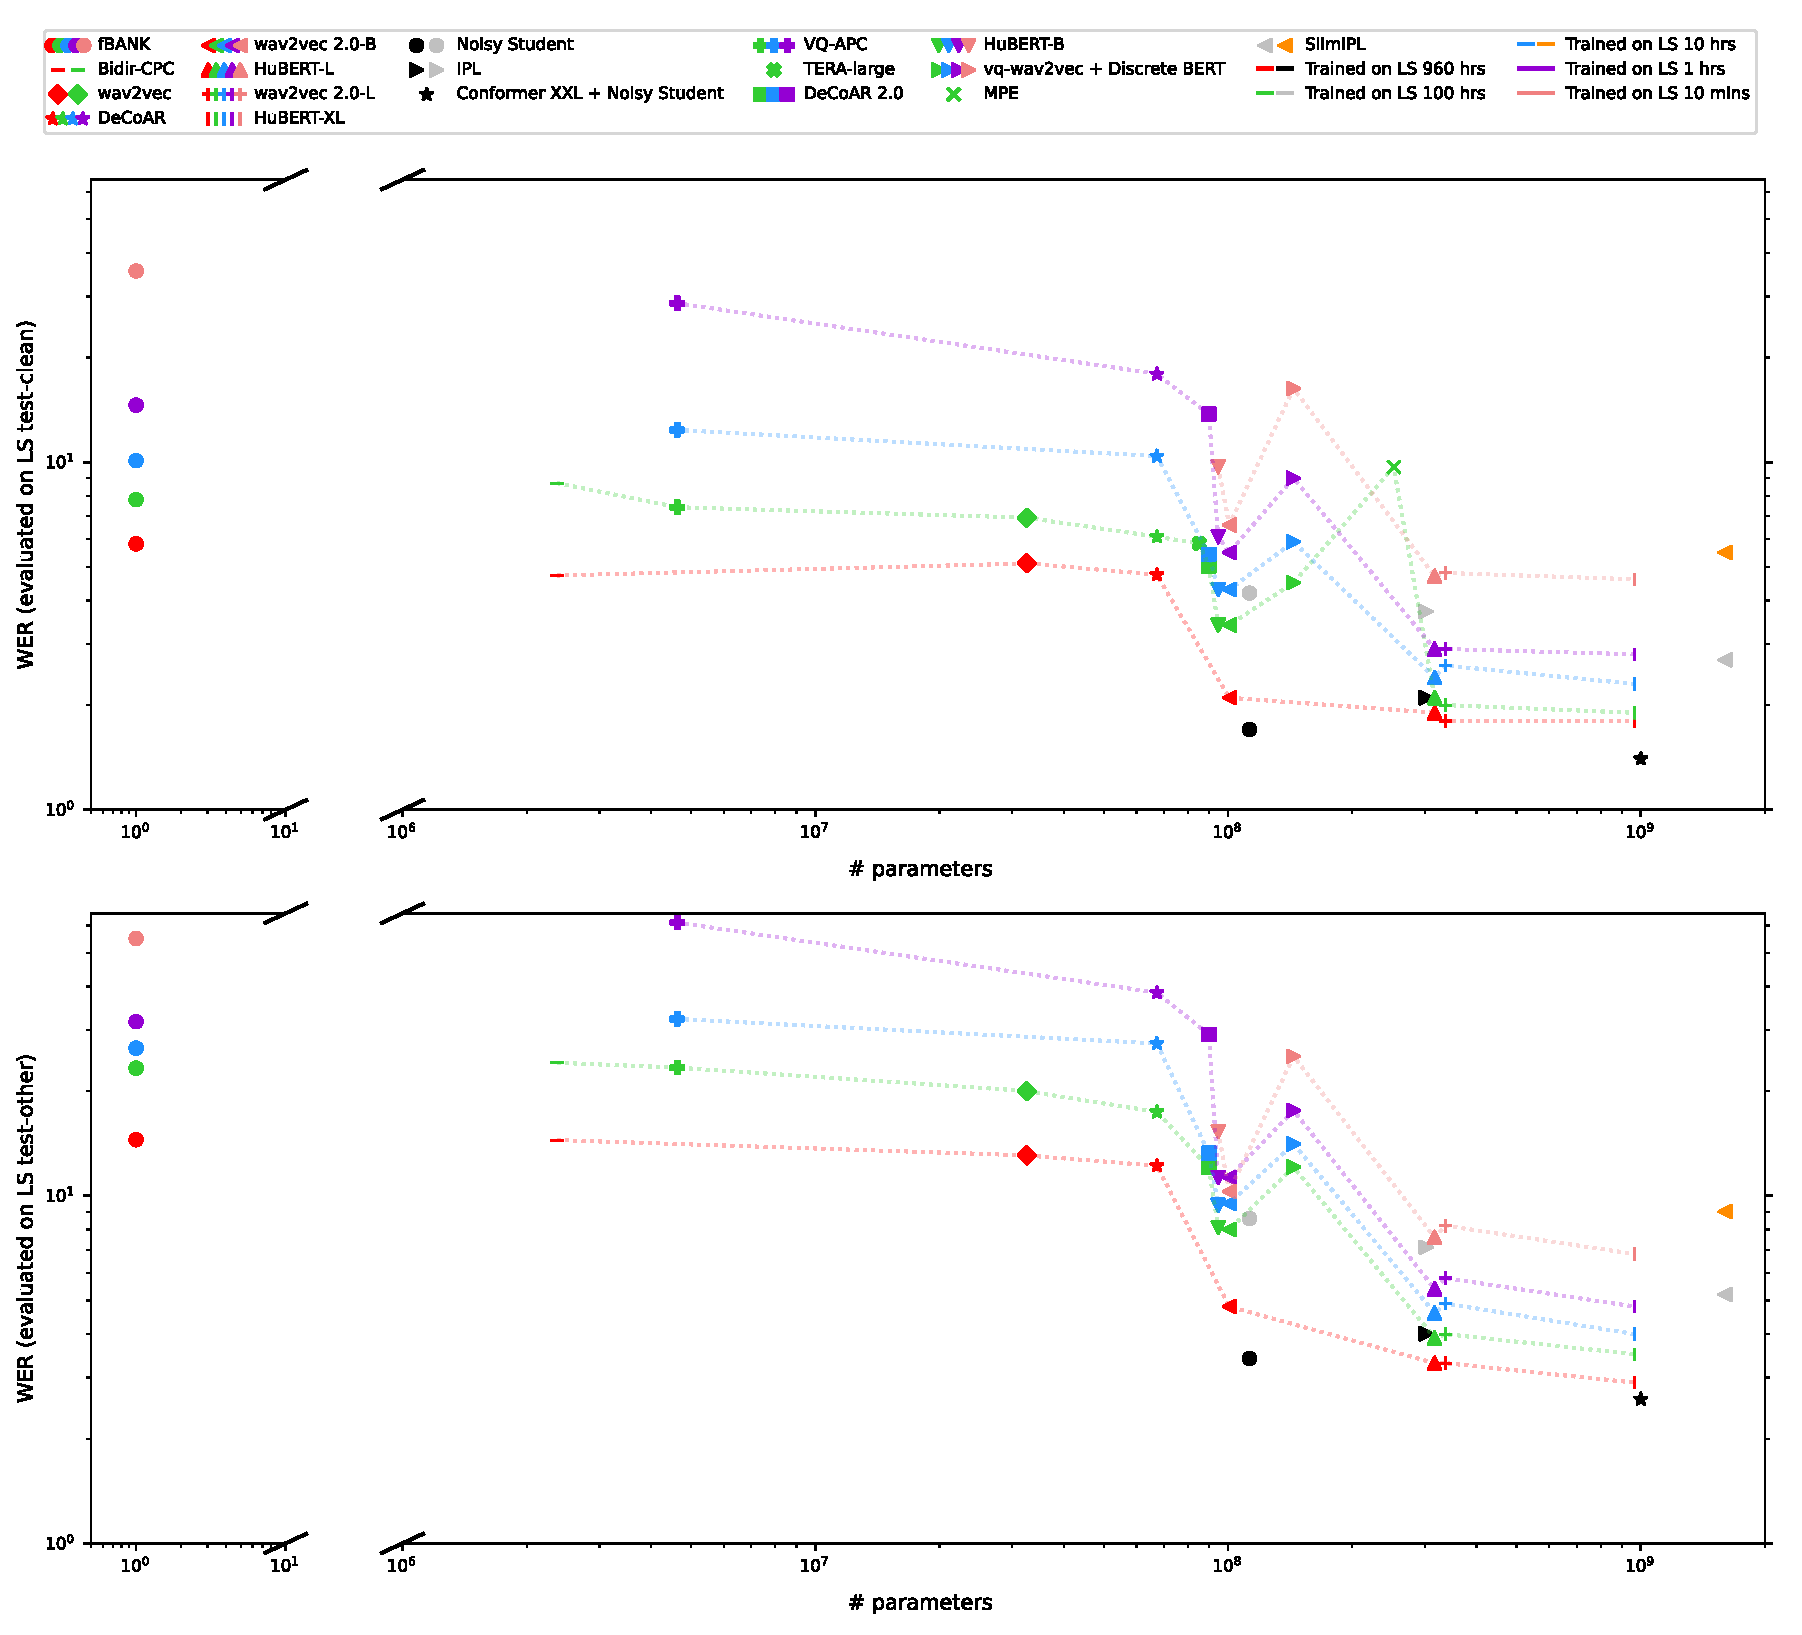
\includegraphics[width=1.0\textwidth]{paper_review/ls-test-clean-other.pdf}
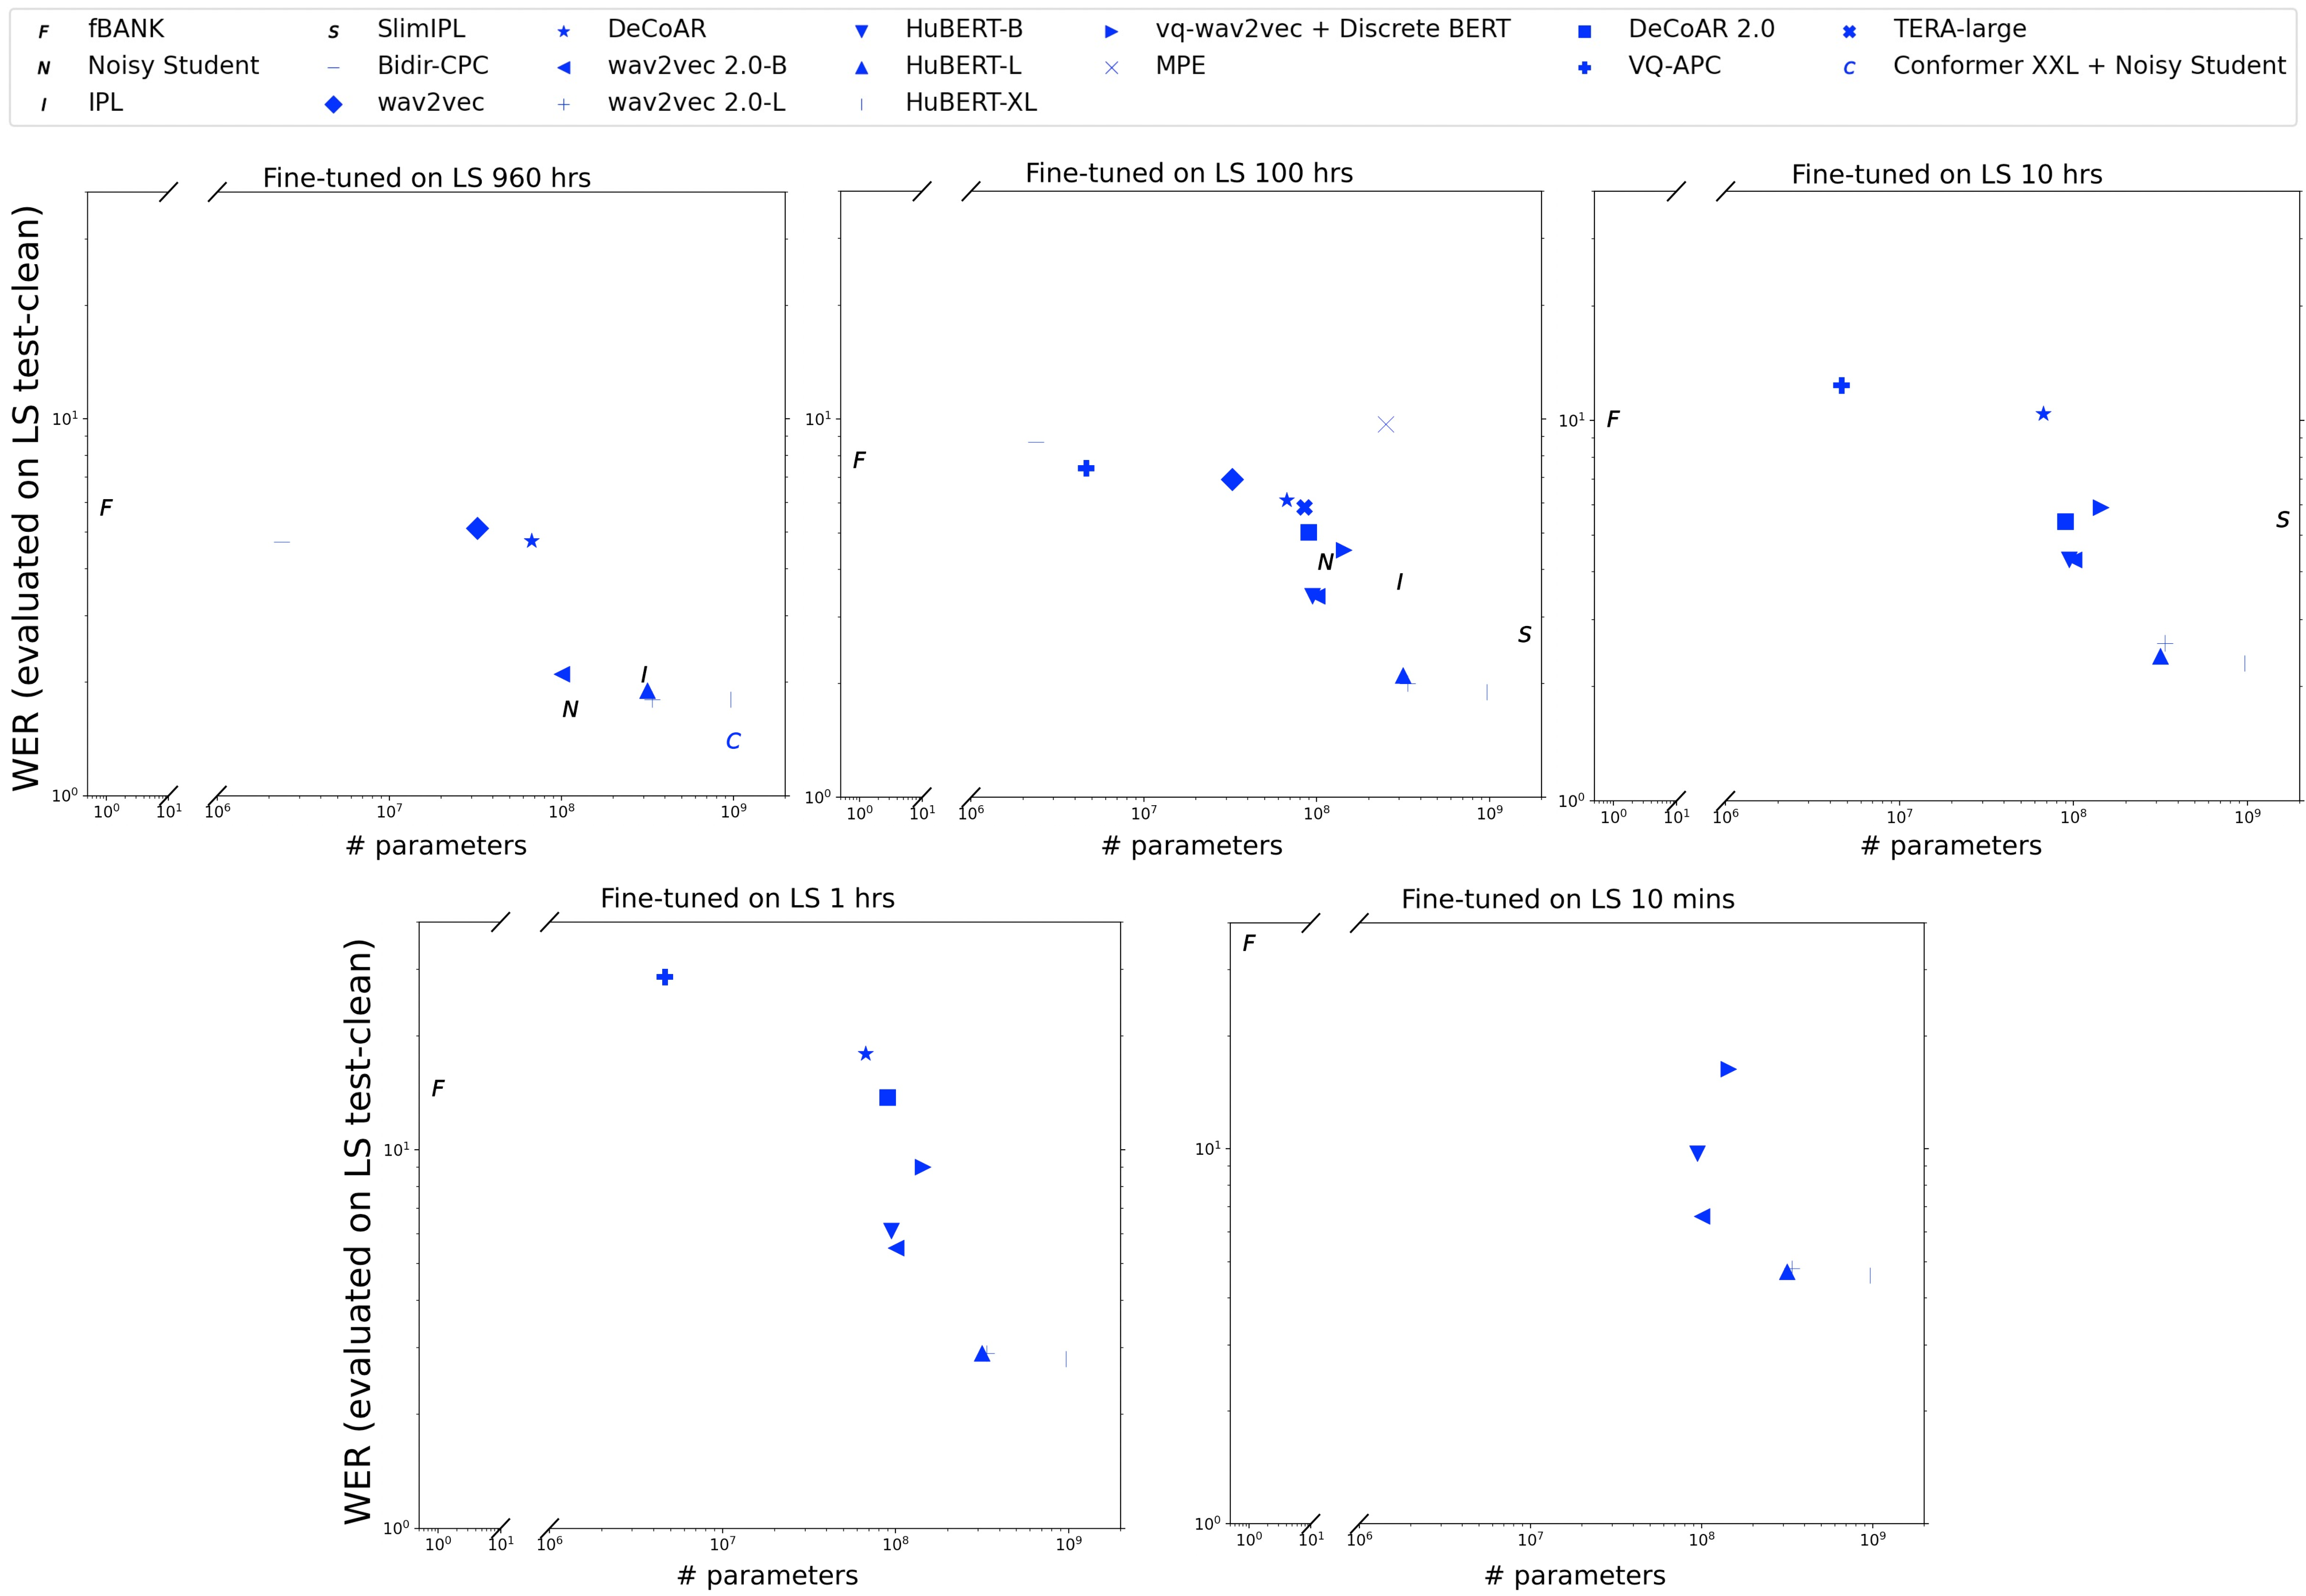
\includegraphics[width=0.9\textwidth]{paper_review/ls-test-clean-v2.pdf}
\caption{SSL performance on ASR WER (vertical axis) evaluated with
LS \textit{test-clean} split. Techniques are sorted based on the number of
model parameters along the horizontal axis. Markers in blue correspond to models initialized with various SSL
techniques and then fine-tuned using 960, 100, 10, 1 hour(s), and 10 minutes
respectively. The 960-hour training set is the aggregation of
\textit{train-clean-100}, \textit{train-clean-360}, and
\textit{train-other-500} splits. The 100-, 10-, 1-hour, and 10-minute sets
leverage \textit{train-clean-100} or its sampling, except for Bidir-CPC, which
samples 10\% of the training examples from the entire 960-hour corpus. For simplicity,
several SSL techniques are appended with suffixes \textit{B}, \textit{L},
\textit{XL}, or \textit{XXL} indicating the \textit{Base}, \textit{Large},
\textit{X-Large}, or \textit{XX-Large} variants specified in the original
publication. We also compare with baselines including the log mel filterbank (fBANK) and semi-supervised, self-training
approaches (iterative pseudo labeling (IPL)~\cite{xu2020iterative}, 
slimIPL~\cite{likhomanenko2020slimipl}, noisy student~\cite{park2020improved}). These approaches are visualized in black. Also, note that the current state of the art---conformer XXL + noisy student~\cite{zhang2020pushing}---is a combination of self-training and SSL techniques. Given the
diversity of the listed methods in experiment settings (e.g., pre-training corpora
and objectives, whether a language model is used in decoding, whether model
parameters are frozen in fine-tuning), readers should be careful that the superiority
of methods cannot be decided only based on lower WER numbers.}
\label{fig:asr_result_no_limit}
\end{figure*}


\subsection{Benchmark results and discussion} \label{sec:benchmark} 
Given the diversity of datasets and downstream tasks used to evaluate SSL
techniques in the literature, it is infeasible to discuss all 
experiment settings in this survey. Hence, due to their wide adoption for
experiments conducted by studies in both SSL and the speech community in
general, we focus first on ASR on the LS dataset to understand the
efficacy of SSL. We examine SSL techniques which report ASR results on the LS
\textit{test-clean} split, and summarize the published WER in
\cref{fig:asr_result_no_limit}. The ASR models were obtained first by using
unlabeled speech to pre-train a model with each SSL technique. The model was
then fine-tuned on labeled data by utilizing a supervised training objective.
Respectively, 960, 100, 10, 1 hour(s), and 10 minutes of labeled LS training data
were used for fine-tuning, as indicated in different panels of
\cref{fig:asr_result_no_limit} (see
the caption of \cref{fig:asr_result_no_limit} for more details).
Semi-supervised methods such as self-training, where a model is first trained
on labeled data to annotate unlabeled speech, and then subsequently trained on
combined golden and self-annotated label-speech pairs, are gaining popularity
in the speech community and have yielded competitive results. For comparison, we also
show performance from such methods (iterative pseudo labeling 
(IPL)~\cite{xu2020iterative}, slimIPL~\cite{likhomanenko2020slimipl}, noisy 
student~\cite{park2020improved}), as well as the current state of the art---conformer XXL + noisy
student~\cite{zhang2020pushing}---which augments SSL with various advanced
techniques including self-training. Furthermore, we illustrate in the figure
the performance of a baseline system \cite{yang21c_interspeech} based on log mel filterbank (fBANK), which is one of the most commonly used features designed by domain experts.
As observed in the figure, most SSL techniques outperform fBANK
features, and with the growing investment in model size, better performance is
achieved. The largest ones, such as wav2vec 2.0-L and HuBERT-L/XL, yield
% results competitive to the state of the art 
  competitive results                         % AMH: check
when the entire 960-hour of labeled data is used in
training/fine-tuning. The benefit of SSL, especially models with more parameters
like wav2vec 2.0 and HuBERT, becomes more evident when the labeling resources
become scarce. Compared to popular semi-supervised methods such as IPL,
slimIPL, and noisy student using 100 hours of labels, wav2vec~2.0 and HuBERT
achieve lower or competitive WERs with 1 hour or even 10 minutes of labeled
examples. The results are highly favorable for low-resource use cases, for instance when
expanding systems to new domains or languages for which large amounts of unlabeled
audio are available, since collecting labels for new conditions is often prohibitively
slow or costly.
% discuss the trend
%[Pick representative tasks and datasets and show the benefit of SSL, e.g., fewer fine-tuning/labeled data is required to achieve better/comparable performance] [talk about trend as well]  The plot suggests that ASR results have been increased significantly with the progress in SSL. Near SOTA performance can be achieved with much fewer training examples.  

In addition to the ASR task, where the current state of the art is achieved by a method
combining SSL pre-training and self-training 
techniques~\cite{zhang2020pushing}, SSL models 
% approach the state of the art 
  are competitive                % AMH: check
in other tasks, including IC,
SID, ASV, and QbE. We summarize the performance of these models and previous
non-SSL methods in \cref{table:sota_performance}. The results suggest that the
benefit of SSL is generalizable among tasks that require encoding 
information such as content, speaker, and semantics. As SSL research
gains more attention, we expect that SSL pre-trained models will 
achieve state-of-the-art results on an increasing number of tasks.

\begin{table}[ht]
  \centering
  \footnotesize
  \caption{Tasks where the state of the art is models with SSL pre-training.}
  \label{table:sota_performance}
  \renewcommand*\arraystretch{1.2}
  \begin{tabular}{llllll}  
    \toprule
    Tasks & Dataset & non-SSL & SSL \\
    \midrule
    ASR (WER $\downarrow$) & LS test-clean/other & 2.1/4.0 \cite{xu2020iterative} & 1.4/2.6 \cite{zhang2020pushing} \\ \hline
    IC (Acc $\uparrow$) & FSC & 98.8 \cite{lugosch19_interspeech} & 99.3\cite{chen2021unispeechsat} \\ \hline
    SID (Acc $\uparrow$) & VoxCeleb1 & 94.8 \cite{hajibabaei2018unified} & 95.5 \cite{chen2021wavlm} \\ \hline
    ASV (EER $\downarrow$) & VoxCeleb1 & 3.1 \cite{hajavi2021siamese} & 2.4 \cite{wang2021fine} \\ \hline
    QbE (MTWV $\uparrow$) & QUESST (EN) & 10.6 \cite{rodriguez2014gtts} & 11.2\cite{chen2021unispeechsat} \\

    %wav2vec-c
    %wav2vec-c \cite{sadhu21_interspeech} & Alexa-10k & ASR & \makecell[l]{Alexa-eval} & \makecell[l]{Alexa-eval} & \checkmark & 1k hrs \\ \hline
    %UniSpeech-SAT \cite{chen2021unispeechsat} & \makecell[l]{LL 60k hrs\\\;\;\;+ GigaSpeech-10k\\\;\;\;+ VP-24k} & Multi & SUPERB & SUPERB & \checkmark & Check SUPERB \cite{yang21c_interspeech} paper for details \\ \hline
    %WavLM \cite{chen2021wavlm} & \makecell[l]{LL 60k hrs\\\;\;\;+ GigaSpeech-10k\\\;\;\;+ VP-24k} & Multi & SUPERB & SUPERB & \checkmark & Check \cite{yang21c_interspeech} for details \\ \hline
    %\multirow{4}{*}[0mm]{XLS-R \cite{babu2021xlsr}} & \multirow{4}{*}[0mm]{\makecell[l]{VP-400k + MLS\\\;\;\;+ CV-dataset-7k + VL\\\;\;\;+ BBL}} & ASR & VP, MLS, CV-dataset, BBL, LS & VP, MLS, CV-dataset, BBL, LS & - & \multirow{4}{*}[0mm]{Check \cite{babu2021xlsr} for details} \\ \cline{3-6}
    %& & SID & VoxCeleb1 & VoxCeleb1 & \checkmark & \\ \cline{3-6}
    %& & ST & CoVoST-2 & CoVoST-2 & \checkmark & \\ \cline{3-6}
    %& & LID & VL & VL & - & \\ \hline

    \bottomrule
  \end{tabular}
\end{table}

Despite the obvious trend of increasing performance as more parameters and SSL
pre-training data are being used, numbers in \cref{fig:asr_result_no_limit} 
and \cref{table:sota_performance} are less comparable than might be expected.
The task performance is obtained from the original papers and is often
achieved with different downstream fine-tuning recipes, including various
language models (used in the ASR system), prediction heads (networks added to
SSL for downstream inference), or choices between fine-tuning the whole
networks or freezing the SSL encoders. For example, in the ASR task, HuBERT-L
and wav2vec~2.0-L leverage Transformer as their language model, while a 4-gram
language model trained on LS is used in DeCoAR~2.0. The lack of common and
established mechanisms to evaluate SSL techniques in downstream applications
makes it difficult to compare techniques fairly and understand their
capabilities. To address this challenge, there are increasing efforts to establish
benchmarks with shared downstream tasks, datasets, and downstream recipes. Such
efforts include SUPERB~\cite{yang21c_interspeech}, 
LeBenchmark~\cite{evain21_interspeech}, ZeroSpeech~\cite{dunbar2020zero},
HEAR \cite{pmlr-v176-turian22a},
NOSS~\cite{shor20_interspeech}, and HARES~\cite{wang2021towards}. 

SUPERB~\cite{yang21c_interspeech} is a benchmarking platform that allows the
SSL community to train, evaluate, and compare speech representations on
diverse downstream speech processing tasks, from acoustic and speaker identity
to paralinguistic and semantics. SUPERB consolidates downstream recipes to
focus on common and straightforward settings (e.g., prediction head
architectures, language models, hyperparameter spaces) to facilitate generalizable
and reproducible benchmarking of SSL techniques. SUPERB also encourages
researchers to innovate for efficient use of model parameters and computation
resources 
to democratize SSL beyond race among Big Tech.   % AMH: what does this mean?
LeBenchmark~\cite{evain21_interspeech} shares a vision similar to SUPERB and provides a
reproducible framework for assessing SSL in French with ASR, spoken language
understanding, speech translation, and emotion recognition. 
ZeroSpeech~\cite{dunbar2020zero} (described in more detail in \cref{zero_speech})
challenges the scientific community to build speech and language understanding
systems using zero expert resources 
%with the ultimate goal of bringing the systems to the services 
for millions of users of ``low-resource" languages.
%or in abnormal condition (dyslexia, autism, etc). ZeroSpeech offers evaluation for independent units in the system as well aggregation of multiple components. 
SSL techniques are also benchmarked with the ZeroSpeech 
challenge~\cite{tjandra20_interspeech, niekerk20b_interspeech}. Apart from the speech
community, researchers have also established HEAR (holistic evaluation of audio
representations) \cite{pmlr-v176-turian22a}, NOSS (non-semantic
speech benchmark)~\cite{shor20_interspeech}, and HARES (holistic audio
representation evaluation suite)~\cite{wang2021towards} to benchmark audio
representations. These efforts promote the creation of an audio embedding
that is as holistic as the human ear in interpreting speech, environmental
sound, and music. Given the significant need to understand and compare SSL techniques
fairly and comprehensively, we expect SSL benchmarking to remain an
active research area.

%SUPERB motivation: consolidating evaluation recipes to understand the capability of various SSL in a fair way. SUPERB designates the architectures of prediction heads for each downstream tasks [common architectures] [frozen] [generalizable, comparable, reproducible results]. [Results on tasks with such constraint conditions (mainly SUPERB but also from literatures imposing similar constraint).] [discussion on the results - competitive performance with simple downstream recipes] [More challenges, ZeroSpeech, HEAR ...]



%Librispeech 100h-960h \\
%Libri-light 10m, 1h, 10h - 60k \\
%SUPERB \\
%Add more
%Hear 2021 Challenge? (focus on audio, not only speech)




                                               
% %!TEX root = ../thesis.tex

\section{Analysis of Self-Supervised Representations}
\label{analysis}

% {\color{blue} Katrin}\\
The previous sections have shown how self-supervised learning can result in
powerful representations that provide a robust starting point for several
downstream tasks. It is natural to ask if we can gain an even deeper
understanding of the nature of these representations, in order to further
optimize them or apply them to different problems.
What is the information encoded in these representations? How robust are they
to distributional shifts, and how dependent are they on the size of the
training data? Do they generalize across languages? What are the key
ingredients for training powerful representations: input data, network
architecture, training criterion, or all three? Can we predict their
performance on downstream tasks from their training behavior? This section
tries to answer these questions by summarizing several studies that analyze
self-supervised representations.

\subsection{Information content}

In \cite{pasad_layerwise_2021} wav2vec~2.0 representations were analyzed with
respect to their acoustic-linguistic information content at different
network layers. Three different mechanisms were used for this
purpose. The first of these is canonical correlation analysis (CCA),
which computes similarity scores between two continuous vectors
based on the maximum correlation of their linear projections.  These
can be used to judge the similarity of embeddings at different layers
with each other, with standard acoustic representations such as mel
filterbank features, or word embeddings derived from text. The second
method clusters continuous representation vectors and computes the
discrete mutual information between cluster IDs and phone or word
labels. The third method involves probing tasks: representation
vectors extracted from the network are used to perform simple
downstream tasks, in particular determining whether two acoustic segments
correspond to the same word, and a standard benchmark of 11 word
similarity tasks~\cite{faruqi14}. These are mostly used to gauge the
amount of lexical information present in the embeddings.  Using this
battery of tests the authors compared pre-trained models of varying
sizes as well as models fine-tuned for ASR. They found that pre-trained
models show an autoencoder-style behavior, with early layers showing
strong similarity with input features, intermediate layers diverging
more, and final layers reverting back to higher similarity with input
features and early layers. Generally, the earlier layers in wav2vec~2.0 
models encode acoustic information. The next set of layers encodes
phonetic class information, followed by word meaning information,
before reverting back to encoding phonetic/acoustic information. Thus,
extracting representations from the last layers for tasks that require
phonetic or word-related information may not be the best
strategy. Indeed, the authors of \cite{baevski2021unsupervised} show that a
phone classifier trained on each of the 24 frozen layers of a wav2vec~2.0 model
showed the lowest phone error rates
for layers 10--21 and higher error rates for the other layers. 
\cite{pasad_layerwise_2021} further show that fine-tuning the pre-trained model with a
character-level CTC training criterion changes the behavior of the
last layers (especially the final two layers), breaking the
autoencoder-style behavior and focusing the information encoded in the
last layers on orthographic-phonetic and word information. 

The peaking of class-relevant information in intermediate layers seems to be
common across different self-supervised learners and different modalities. In
an analysis of text-based Transformers trained with a masked language model
criterion~\cite{voita2019} observed a similar compression plus reconstruction
pattern. Interestingly, similar network behavior was also recently described
for self-supervised learners in computer vision: using a contrastive
self-supervised learner (SimCLR) that optimizes for augmentation invariance,
\cite{grigg2021self} show that it is the intermediate representations that most
closely approximate information learned in a supervised way, i.e., they
provide more class information than the representations from final layers. This
is similar to the findings described above for wav2vec~2.0 without fine-tuning,
where intermediate layers provide more information about phone and word
classes.

Self-supervised representations may encode other information besides phonetic
classes or words, for example, channel, language, speaker, and sentiment
information. 
\edit{It is shown that the per-utterance mean of CPC features captures speaker information to a large extent\cite{van2021analyzing}.}
Location of information pertaining to speakers vs.\ language classes was
analyzed in \cite{ling20odyssey} for a 12-layer BERTphone model. This model
combines a self-supervised masked reconstruction loss with a phone-based CTC
loss to produce representations	for speaker recognition and language
identification. By	analyzing the weights	of a linear combination	of layer
representations for these two downstream tasks, it was	shown that language
recognition draws on representation	from higher layers (peaking at layer~10)
whereas speaker recognition benefited from layers at positions 6, 9, and 12.
This may indicate that language recognition relies more on higher-level
phonetic information whereas speaker recognition uses a combination of
acoustic and phonetic information. In a recent study~\cite{chen_wavlm_2021} the
same technique was used to identify layer contributions for the downstream
SUPERB benchmark tasks in the WavLM model. For a smaller model (95M parameters)
it was again confirmed that lower layers encode speaker-related information
necessary for speaker diarization and verification whereas higher layers encode
phonetic and semantic information. Another study~\cite{wang2021layersup} used
explicit self-supervised loss at the intermediate layers rather than just the
output layer of a HuBERT model in order to enforce better learning of phonetic
information. The resulting model was indeed better at downstream tasks
requiring information about phonetic content, such as phone recognition, ASR,
and keyword spotting, but worse at speaker-related tasks like speaker
diarization and verification. 

%Hung-yi Lee: My group also has a paper analyzing the attention of self-supervised speech model (https://arxiv.org/abs/2006.03265). I will include some findings in this subsection later.
Most self-supervised learning approaches rely on a Transformer architecture for
the representation model. In \cite{AnalyzeAttention} the attention patterns in
generatively trained Transformer representation models were analyzed.
Self-attention heads were grouped into three categories: diagonal, vertical,
and global. It was found that the diagonal head focuses on neighbors and is
highly correlated with phoneme boundaries, whereas the vertical head focuses on
specific phonemes in the utterance. Global heads were found to be redundant as
removing them resulted in faster inference time and higher performance.

\subsection{Training criterion}
In \cite{chung2021}, representations based on different training criteria
(masked predictive coding, contrastive predictive coding, and autoregressive
predictive coding) were compared  and analyzed with respect to the correlation
between their training loss and performance on both phone discrimination and
speaker classification probing tasks. It was observed that the autoregressive
predictive coding loss showed the strongest correlation with downstream
performance on both tasks; however, models were not further analyzed
internally. An evaluation of the similarity of representations trained
according to the three criteria above (but with different architectures and
directionality of contextual information) also showed that it is the training
criterion that most influences the information encoded in the representations,
not the architecture of the learner or the directionality of the input. 

A similar insight was obtained in \cite{zhou2020}, which compared vq-vae and
vq-wav2vec with respect to their ability to discover phonetic units.
The vq-vae model extracts continuous features from the audio signal; a
quantizer then  maps them into a discrete space, and a decoder is trained to
reconstruct the original audio conditioned on the latent discrete
representation and the past acoustic observations. By contrast, vq-wav2vec
predicts future latent discrete representations based on contextualized
embeddings of past discrete representations, in a CPC-style way. The models
were evaluated according to their ability to discover phonetic units (as
measured by phone recognition error rate on TIMIT, and the ZeroSpeech ABX task
(see \cref{sec:zero} for more details)), and it was found that the predictive vq-wav2vec
model fared better than the autoencoder-like vq-vae model, most likely due to
its superior ability to model temporal dynamics.

\subsection{Effects of data and model size}
\label{subsec:modelsize}

How does the performance of self-supervised models change in relation to the
amount of training data, and in relation to the size (number of parameters) of
the model?
Several studies have demonstrated better downstream performance when using
larger datasets~\cite{rivi20, kawakami2020learning, chen_wavlm_2021}. For
example,
\cite{kawakami2020learning} compared representations learned by a bidirectional
CPC model from the standard 960 hour LS corpus and a corpus of 8,000 hours of
diverse speech from multiple sources.\textsuperscript{\ref{footnote:CPC-8k}}
Not surprisingly, an ASR model trained on top of these representations
performed better when representations were learned from the larger dataset. 
Although the precise relationship between data size and performance has not
been quantified, we can assume that it follows a law of diminishing returns (or
power law), 
similar to observations for most data-intensive machine learning tasks.
In addition to the size of the dataset, the diversity of the data also seems
to play a role, although this was not quantified in this study. However, recent
experiments with larger and more diverse data collections~\cite{chen_wavlm_2021}
confirm this assumption, as do 
explicit investigations of domain shift robustness (see
\cref{subsec:robustness} below). 

\edit{The relation between model sizes and downstream performances have also been investigated \cite{pue2021scaling,versteegh2015zero}.}
Using the Mockingjay 
model~\cite{liu_mockingjay_2020}, the authors in \cite{pue2021scaling} attempt to establish a relationship between
model size and self-supervised \ensuremath{L_1} loss and demonstrate that it approximately
follows a power law. Model size and accuracy on downstream phone
classification and speaker recognition tasks are positively correlated but do not
exactly follow a power law; rather, the accuracy saturates as models increase in
size, possibly due to the lack of a corresponding expansion in training data
size.

\subsection{Robustness and transferability}
\label{subsec:robustness}

It is well known that traditional speech features like MFCCs lack
robustness against environmental effects such as additive noise,
reverberation, accents, etc., that cause differences in the distributions of
speech features.
Do pre-trained representations offer greater robustness against distributional
shifts? 
One study~\cite{kawakami2020learning} compared pre-trained
representations from a CPC model against MFCCs and 
found pre-trained representations to be more robust to mismatches between
training and test data. The 
training data consisted of clean, read speech (LS)
whereas test data consisted of the Switchboard corpus and TED talks. The
distributional shifts here may stem from both the acoustics (microphone, room
reverberation) as well as
lexical effects related to topic and style, as well as differences in speaker
characteristics such as accent. 
Similar problems were also investigated using HuBERT and wav2vec~2.0 models in
\cite{chang2021exploration}.
In \cite{robustw2v2} domain effects were studied in greater detail using 
datasets from six different domains. In particular, the authors focused on the
usefulness of adding out-of-domain data to pre-training. The general
conclusions are that pre-training on more and diverse domains is preferable:
models pre-trained on more domains performed better than those pre-trained on
fewer when tested on held-out domains, regardless of which additional
labeled data was used for fine-tuning. Adding in-domain unlabeled data---if
available---to pre-training improves performance robustly; however, even
out-of-domain unlabeled data is helpful and closes  66--73\% of the performance
gap between the ideal setting of in-domain labeled data and a competitive
supervised out-of-domain model. 
 
In \cite{rivi20} the effectiveness of CPC-trained representations for
phone discrimination tasks was compared across several languages. It
was found that representations pre-trained only on English successfully
enabled phone discrimination in 10 other languages, rivaling
supervised methods in accuracy in low-data regimes (1h of labeled data
per language). Thus, self-supervised pre-training enables the model to
learn contextualized speech features that generalize across different
languages. In \cite{conneau20xling}, a wav2vec~2.0 model was trained on data
from multiple different languages and different corpora (Babel, Common Voice,
and multilingual LS)
jointly, followed by fine-tuning for each individual language. The largest
model covers 53 languages in total
and consists of 56,000 hours of speech. Compared to monolingual pre-training,
even smaller models trained on only ten languages improve performance
substantially on a downstream character-based ASR task. Low-resource languages
with little labeled data improve the most under this training regime.
Multilingual representations also resulted in competitive performance (lower
character error rate than monolingual representations) for languages not
present in the training dataset, again showing that unsupervised pre-trained
representations can learn generic features of the speech signal that generalize
across different languages. The study also found that sharing data from closely
related languages is more beneficial than combining distant languages. An
analysis of language clusters in the shared discrete latent representation
space revealed that similar languages do indeed show a higher degree of sharing
of discrete tokens. 
Finally, one might ask whether the interpretation of representations extracted
from different layers of a self-supervised models also generalizes to the
multilingual setting. Experiments in \cite{baevski2021unsupervised} on phone
recognition in eight languages based on the different layers of the
multilingual wav2vec~2.0 XLSR-53 model indicate that this is indeed the case:
phone error rates showed the same pattern as in the monolingual (English)
scenario, with lower phone error rates for middle layers as opposed to
earlier/later layers. 





   % TODO (JDH): Compilation errors completed until here
                                               % TODO (JDH): Currently changing citation keys here

% %!TEX root = ../thesis.tex

\section{From representation learning to zero resources}
\label{sec:zero}

% {\color{black} Reviewer: TNS, Abdo, Hung-yi Lee }\\
% \kl{We discussed in our last meeting that I would add a pointer in this section to the acoustic word embedding section.  However, I'm not quite sure what the right spot for it is, so waiting for this section to stabilize a bit more first.}


In the SSL framework, speech representations can be
learned and used in various downstream tasks to achieve competitive, robust,
and transferable performance, as shown in
\crefrange{section:benchmark}{analysis}. 
However, labeled data is still required. 
For example, in ASR, utterances and their manual transcriptions are needed to learn downstream models or fine-tune representation models. 
Can a model learn without any labeled data? 
In \cref{secsec:unpaired}, we show how to learn ASR models without any paired audio and text and how SSL improves the framework.
In addition, many languages have no writing system. 
In \cref{subsec:zero}, the SSL representation is further used in scenarios where text data is unavailable.

\subsection{Unpaired text and audio} \label{secsec:unpaired}
% What are we going to do % how to match
%In the self-supervised learning framework, speech representations can be learned and used in the downstream tasks, but some labeled data for finetuning is needed.

\begin{sidewaystable}
\centering
\caption[Performance of models within unsupervised ASR.]{
	Unsupervised ASR.
	TIMIT numbers are phoneme error rates (PER), while the numbers for
	LibriSpeech are word error rates (WER).
	SWC $=$ spoken word classifier, ST $=$ speech translation.
	All speech and text are in English if not specified. 
	\textcolor{black}{The references in the table are sorted according to the date of publication.}}
	\label{fig:unsupervisedASR}
	\resizebox*{\textwidth}{!}{%
	{\renewcommand*\arraystretch{1.4}}
	\begin{tabular}{cllllll}
	\toprule
	Reference & Speech representation & Speech segmentation  & Token & Mapping approach & Refinement  & Results  \\ 
	\midrule
	\parencite{liu_completely_2018}& Audio word2vec~\parencite{wang_segmental_2018} & Oracle & Phoneme & \edit{Adversarial Training~\parencite{gulrajani_improved_2017}} & - & TIMIT (PER): 63.6\%  \\ %Submitted on 1 Apr 2018
	\midrule
	\parencite{chung_unsupervised_2018} & Speech2vec~\parencite{chung_speech2vec_2018} & BES-GMM~\parencite{kamper_segmental_2017} &  Word2Vec & \edit{Adversarial Training~\parencite{conneau_word_2018}} & Self-training & SWC (Acc): 10.9\%  \\ %Submitted on 18 May 2018
	%https://arxiv.org/pdf/1805.07467.pdf %The text embeddings were obtained by training Word2Vec on the transcriptions using the fastText implementation without subword information [3].
	\midrule
	
	\parencite{chung_unsupervised_2019a} & \tabincell{l}{Speech2vec\\(English)} & Oracle & \tabincell{c}{Word2Vec\\(French)} & VecMap~\parencite{artetxe_robust_2018} & \tabincell{l}{LM rescore,\\sequence DAE} & ST (BLEU): 10.8\%   \\ %[Submitted on 4 Nov 2018]
	\midrule
	
	\parencite{yeh_unsupervised_2019} & MFCC & GAS~\parencite{wang_gate_2017} & Phoneme & Empirical-ODM~\parencite{liu_unsupervised_2017} & Self-training &  TIMIT (PER):  41.6\%  \\ %Submitted on 23 Dec 2018
	\midrule

	\parencite{chen_completely_2019} & MFCC & GAS  & Phoneme & \edit{Adversarial Training~\parencite{gulrajani_improved_2017}} & Self-training &  TIMIT (PER):  33.1\%   \\
	\midrule

	\parencite{baevski_unsupervised_2021} & Wav2vec 2.0~\parencite{baevski_wav2vec_2020} & $k$-means & Phoneme &\edit{Adversarial Training~\parencite{gulrajani_improved_2017}} & Self-training & \tabincell{l}{TIMIT (PER):  18.6\%, \\ LibriSpeech (WER): 5.9\%}   \\
	\midrule
	
	\textcolor{black}{\parencite{klejch_deciphering_2022}} & \textcolor{black}{\tabincell{l}{Universal Phone \\ Recogniser}} & - & \textcolor{black}{Grapheme} & \textcolor{black}{Decipherment~\parencite{ravi_deciphering_2011}} & \textcolor{black}{Self-training} & \textcolor{black}{\tabincell{l}{GlobalPhone: 32.5\% to just 1.9\% \\ worse than supervised models} }  \\ %ubmitted on 12 Nov 2021 %m 32.5% to just 1.9% absolute worse than the equivalent fully supervised models trained on the same data
	\midrule
	\textcolor{black}{\parencite{liu_endtoend_2023}} & \textcolor{black}{Wav2vec 2.0~\parencite{baevski_wav2vec_2020} }& - & \textcolor{black}{Phoneme} & \textcolor{black}{Adversarial Training~\parencite{gulrajani_improved_2017}} & \textcolor{black}{Self-training} & \textcolor{black}{LibriSpeech (WER): 6.3\%}   \\
	\midrule

	\textcolor{black}{\parencite{liu_endtoend_2023}} & \textcolor{black}{Wav2vec 2.0~\parencite{baevski_wav2vec_2020}} & - & \textcolor{black}{Grapheme} & \textcolor{black}{Adversarial Training~\parencite{gulrajani_improved_2017}} & \textcolor{black}{Self-training} & \textcolor{black}{LJSpeech (WER): 64.0\%}  \\


	%e MUSE [7] and VecMap [8], n
	%The numbers in the section of unsupervised methods denoted as BLEU score (%) of VecMap /
	%BLEU score (%) of MUSE 10.8 / 6.2
	%11.3 / 7.3
	%https://arxiv.org/pdf/1811.01307.pdf
	\bottomrule
	\end{tabular}}
\end{sidewaystable}



\paragraph{Unsupervised ASR}
% {\color{black} Hung-yi}\\

If only unpaired speech and text are available, that is, the text is not a
manual transcription of speech, can the machine learn how to transcribe speech
into text?
This scenario is called \textit{unsupervised ASR}, and the framework is as
below. 
Given a set of unlabeled utterances $\mathcal{S}=\{S_1, S_2, ..., S_N\}$  and a
set of sentences $\mathcal{Y}=\{Y_1, Y_2, ..., Y_M\}$,\footnote{Note that
the speech and text are not paired, that is, $Y_i$ is not the transcription of
$S_i$.} a mapping function~$F$, which can take an utterance~$S$ as input and
generate its transcription, is learned from data. 
\Cref{fig:unsupervisedASR} summarizes recent work on unsupervised ASR,
including the speech representation used, the algorithm used to learn the
mapping without supervision, and the results. Below, we will discuss these
methods in more detail.


Adversarial training~\parencite{goodfellow_generative_2014,arjovsky_wasserstein_2017, gulrajani_improved_2017} is one common way to learn such a 
mapping function. 
The framework includes a discriminator and a generator.
The mapping function~$F$ plays the role of the generator, which takes speech utterances as input and outputs text.
The discriminator learns to distinguish real text from the generated
output; the generator learns to ``fool'' the discriminator.
The generator and the discriminator are trained in an iterative, 
interleaved way. 
After the training, the generator serves as the speech recognition model.
\edit{
There is a large amount of work using gradient penalty in the objective of training discriminators~\parencite{liu_completely_2018,chen_completely_2019,baevski_unsupervised_2021,liu_endtoend_2023}, which is inspired by Improved Wasserstein Generative Adversarial Network (WGAN)~\parencite{gulrajani_improved_2017}.
}
\textcolor{black}{
Other ways to map speech and text include via segmental empirical output distribution matching (segmental empirical-ODM)~\parencite{yeh_unsupervised_2019} and decipherment algorithm~\parencite{klejch_deciphering_2022}.}

% Difficulty of unsupervised ASR (v.s. unsupervised MT)
Success in unsupervised neural machine translation
(MT)~\parencite{artetxe_unsupervised_2018, conneau_word_2018, lample_unsupervised_2018}
has inspired innovative exploration of various unsupervised ASR algorithms.
If learning a translation model from unaligned sentences in two languages is
possible, considering speech and text as two different languages, learning the
mapping relationship from speech space to text space without an alignment 
% is not impossible.
  should likewise be possible.   % AMH: check
However, there are differences between unsupervised MT and unsupervised
ASR.
In unsupervised MT, most discrete source tokens can be mapped to specific
target tokens representing the same meaning. 
However, because speech has segmental structures, in unsupervised ASR, each text
token maps to a segment of consecutive acoustic features of variable length in
an utterance.
The generator is supposed to learn the segmental structure of an utterance
because information like token boundaries is not directly available.
This makes unsupervised ASR more challenging than unsupervised MT.

% how to represent audio
For unsupervised ASR to be feasible, the common idea is to make the speech and text units close to each other.
For the text side, word sequences can be transformed into phoneme sequences if a lexicon is available. 
On the other hand, we must first convert the speech signal into something close to phonemes. 
To achieve that, most studies on unsupervised ASR use a phoneme
segmentation module before the generator to segment utterances into
phoneme-level
segments~\parencite{liu_completely_2018,chen_completely_2019,yeh_unsupervised_2019}. 
A representation vector or a token then represents each phoneme-level segment. 
It is easier for the generator to map each segment-level representation 
or token to the correct phoneme when the representation or token is highly correlated to the phonemes.
Wav2vec-U~\parencite{baevski_unsupervised_2021} selects the input feature from different layers of wave2vec~2.0~\parencite{baevski_wav2vec_2020}.
The selection criterion is based on analysis of the phonetic information in each layer.
\textcolor{black}{
If a universal phone recognizer trained from a diverse set of languages is available, it is another way to transcribe speech into phone-level tokens~\parencite{klejch_deciphering_2022}.}
Another series of work is to transform a word into a word embedding. 
\parencite{chung_unsupervised_2018,chung_unsupervised_2019a} use adversarial training to map the word-level
speech embedding space~\parencite{chung_speech2vec_2018} to the word embedding space
and achieve promising performance on spoken word classification, speech
translation, and spoken word retrieval.
\Cref{fig:unsupervisedASR} summarizes the various ways to segment speech and represent speech and text in each reference.  

%Hung-yi Lee: I comment this paragraph first.
\begin{comment}
%Hung-yi Lee: This paragraph is not finished yet.
\TNS{if we are limited on space,we can consider removing some of the detail of the various algorithms}
\TNS{split into 2 sentences, also have a connection to the previous para}
\parencite{liu_completely_2018} is the first work to successfully achieve unsupervised
phoneme recognition by first clustering phoneme-level
embeddings~\parencite{chung_audio_2016,wang_segmental_2018} into a set of
tokens and then using GAN to learn the mapping relationship between tokens and
phonemes. 
However, in \parencite{liu_completely_2018}, oracle phoneme segmentation is still
required to get reasonable performance. 
\parencite{chen_completely_2019,yeh_unsupervised_2019} uses gate activation signals
(GAS)~\parencite{wang_gate_2017} to get the phoneme-level segmentation, which is
unsupervised. 
%However, the loss term in~\parencite{yeh_unsupervised_2019} includes an empirical average over all segments inside a logarithmic function, which can be biased if we sample this empirical average by a mini-batch average. \parencite{liu2017unsupervised} therefore use an extremely large batch size during training to reduce the biasing problem.
%These problems are handled by another work~\parencite{chen_completely_2019}.
%\parencite{chen_completely_2019} removes the quantization step.
%Compared to~\parencite{yeh_unsupervised_2019}, the discriminator in~\parencite{chen_completely_2019} considers all possible information from the text dataset, not limited to the n-gram local statistics.
%Besides, \parencite{chen_completely_2019} works well with a reasonable batch size, which makes it feasible when the computational resource is limited.
Wav2vec-U~\parencite{baevski_unsupervised_2021} selects the input feature from
different layers of wave2vec 2.0~\parencite{baevski_wav2vec_2020}, a self-supervised
model.
The selecting criterion is the PER by training a linear model in a supervised manner. 
%Should we mention this?
Wav2vec-U uses $k$-means to cluster the selected features, and the boundaries
are drawn whenever the clustered index changes.
%Wave2vec-U tends to generate more segments compared to the oracle phoneme-level segments. For example, their segmentation gives 0.93 precision, the ratio of the oracle phoneme-level boundaries being hit, and 0.38 recall, the ratio of the generated boundaries hit the oracle phoneme-level boundaries.
While Wav2vec-U merges the neighboring segments containing the same predicted
labels in each step of GAN training, this design can be viewed as refining the
segmentation implicitly.  
%Should we mention this?
%At generator output, the wav2vec-U will combine the neighboring predicted posterior containing the same predicted label into a predicted posterior.
\end{comment}

%In \parencite{chung_unsupervised_2018, chung_unsupervised_2019a}, the word boundaries are also generated automatically with speech only. 
%However, \parencite{chung_unsupervised_2018, chung_unsupervised_2019a} need oracle boundaries, therefore not completely unsupervised as the framework proposed in this paper.

% more improvement: iterative training, development 
As shown in \cref{fig:unsupervisedASR}, most studies use
\textit{self-training} to refine the models.
% to achieve better performance.  % AMH: redundant
In self-training, the generator serves as the first-version phoneme recognition model.
Inputting unpaired speech to the generator generates the corresponding
``pseudo transcription''. 
We then view the speech utterances and their pseudo transcriptions as paired
data which we use to train a model in a supervised manner.
Although the pseudo transcriptions have more errors than oracle
transcriptions, experiments show that training models on pseudo
transcriptions still significantly boosts performance compared to the
first-version model.
%With the new model, we can further obtain new transcriptions.
%The iteration will continue until the performance converges. 

%Using performance to end this section.
Wav2vec-U~\parencite{baevski_unsupervised_2021} achieved state-of-the-art results at the time, which suggests that representation learning is
essential for the success of unsupervised ASR.
It achieved an 11.3\% phoneme error rate on the TIMIT benchmark. 
On the LS benchmark, wav2vec-U achieved a 5.9\% \edit{WER} on
\emph{test-other}, rivaling some of the best published systems trained on 960 hours of labeled data from only two years earlier. 
\textcolor{black}{
And wav2vec-U 2.0~\parencite{liu_endtoend_2023} further removes the requirement of the segmentation stage, so the unsupervised ASR model can be learned in an end-to-end style.}
The robustness of wav2vec-U was further analyzed with respect to 
domain-mismatch scenarios in which the domains of unpaired
speech and text were different~\parencite{lin_analyzing_2022}.
Experimental results showed that domain mismatch leads to inferior performance, but a representation model pre-trained on the targeted speech domain extracts better representations and reduces this drop in performance.

%Hung-yi: The technique below is very important. But I think it is fine to ignore this part in a reviewe paper due to space limitation. 
\begin{comment}
In unsupervised learning, how to determine the hyperparameters is an issue. 
In a typical supervised framework, hyperparameter tuning is done by a
development set, which includes labeled data.
In an unsupervised setting, the existence of this kind of development is tricky. %Is tricky a correct term?
The existence of such kind of development set means the presence of the labeled
data.
Therefore, wav2vec-U~\parencite{baevski_unsupervised_2021} develops a new approach to
determine the hyperparameters without a labeled development set. 
%should I provide more details? 
\end{comment}

%Hung-yi: A series of work (most from MS) focuses on meager resources but not wholly unsupervised. Perhaps we have to mention the papers.


\paragraph{ASR-TTS}
%{\color{black} Shinji}\\
%{\color{black} Hung-yi: In the last meeting, we discussed the connection between this section and self-supervised learning. In addition to looking for papers using self-supervision to improve the ASR-TTS framework here, I think there may be another direction. Can we regard this ASR-TTS framework as a kind of self-supervised learning? ASR-TTS is similar to an autoencoder, and the output of ASR is "latent representation". In other words, this section describes a special self-supervised learning method, whose representation is expressed as "text."}\\
%{\color{black} Hung-yi: However, the above idea sounds tricky. In addition, the ``ASR-TTS'' autoencoder is learned by semi-supervised, not self-supervised.}
% AMH: to make the paper more consistent, I recommend changing all $f^{\mathrm{asr}}$ to $f_{\mathrm{asr}}$
Here we describe an alternative approach by which to train an ASR and \edit{text-to-speech (TTS)} system
based on unpaired text and audio. The ASR-TTS framework, which \edit{combines the ASR} and
TTS systems in a cascaded manner,
can be regarded as an autoencoder, where the encoder~$f$
corresponds to the ASR module and the decoder~$g$ corresponds to the TTS module.
In this framework, we consider the intermediate ASR output as a latent
representation; the framework as a whole can be regarded as a variant of
self-supervised learning.\footnote{However, to make this complicated
system work, we often require that data is paired. Therefore, in practice,
ASR-TTS and other methods described in this section are categorized as
semi-supervised learning.}

The ASR-TTS framework can jointly optimize both ASR and TTS \edit{without using paired data}~\parencite{tjandra_listening_2017,hori_cycleconsistency_2019,wang_improving_2020}.
A speech chain~\parencite{tjandra_listening_2017,tjandra_machine_2018} is one 
successful way to utilize audio-only and text-only data to train both
end-to-end ASR/TTS models.
This approach first prepares pre-trained ASR model \edit{
$f_{\mathrm{asr}}(X)$ with acoustic input $X$ and pre-trained TTS model $g_{\mathrm{tts}}(Y)$ with text input $Y$.
By following the TTS system with an ASR system, we generate new 
acoustic feature sequence~$\hat{X}$, which must be close to the original input~$X$.
Thus, we design a loss function $\mathcal{L}_{\mathrm{asr} \rightarrow \mathrm{tts}}(X, \hat{X})$, where $\hat{X}$ is generated by
%and~$\hat{X}$:
%\begin{equation}
%    \mathcal{L}_{\mathrm{asr} \rightarrow \mathrm{tts}} (X, \hat{X}),
%\end{equation}    
%where
\begin{equation}
    \hat{X} = g_{\mathrm{tts}}(f_{\mathrm{asr}}(X)) \enspace .
    \label{eq:asr-tts}
\end{equation}
Thus, we train the ASR model (or both ASR and TTS models) using only
the acoustic input by minimizing $\mathcal{L}_{\mathrm{asr} \rightarrow \mathrm{tts}}$.  
%\begin{equation}
%\hat{\theta}_{\mathrm{asr}} = \arg \min _{\theta_{\mathrm{asr}}} \mathcal{L}(Y, \hat{Y}; \theta_{\mathrm{asr}}, \theta_{\mathrm{tts}}).
%\end{equation}
Note that this approach does not require the supervised text data~$Y$}.
As an analogy to the generative approach in \cref{sec:generative}, the
intermediate ASR output~$\hat{Y}$ can be regarded as the latent representation~$Z$.

The other cycle with the text-only data~$Y$ is also accomplished by the
concatenated TTS-ASR systems:\edit{
\begin{equation}
    \hat{Y} = f_{\mathrm{asr}}(g_{\mathrm{tts}}(Y)) \enspace .
    \label{eq:tts-asr}
\end{equation}
Similarly, this approach does not require the supervised audio data~$X$, and the
intermediate TTS output~$\hat{X}$ can be regarded as the latent representation~$Z$}.
Although this approach initially freezes either the ASR or TTS model, 
extensions of this study~\parencite{hori_cycleconsistency_2019,tjandra_endtoend_2019,baskar_semisupervised_2019}
implement the joint training of both ASR and TTS parameters using 
REINFORCE~\parencite{williams_simple_1992} and straight-through estimators.

An emerging technique uses a well-trained TTS system to generate
speech and text data from text-only data.
This technique is a sub-problem of the TTS-ASR approach formulated in
\eqref{eq:tts-asr} in which we fix the TTS system part and estimate only the ASR
parameters. 
For example, a huge amount of text resources can be obtained from the web
and document archives without corresponding audio data.
%Self-supervised learning in this paper mostly focuses on representation learning perspectives of such unpaired data.
The typical use case scenario of such a text resource for ASR is through \edit{the
language model}. 
We combine the ASR and language model via a noisy channel 
model~\parencite{jelinek_statistical_1997}, a weighted finite state 
transducer~\parencite{mohri_weighted_2002}, or shallow 
fusion~\parencite{gulcehre_using_2015,chorowski_better_2017}.
However, the progress of TTS systems boosted by deep 
learning~\parencite{oord_wavenet_2016,shen_natural_2018} has inspired another interesting and
straightforward research direction: \edit{artificially creating paired text and audio
data $\{\hat{X}, Y\}$ with only text data~$Y$ by generating the corresponding
audio data~$\hat{X}$ with TTS.} %\begin{equation}
%    \{\hat{X}, Y\} \text{ where } \hat{X} = g_{\mathrm{tts}} (Y).
%\end{equation}
The most straightforward approach is to simply use multi-speaker TTS to
generate the waveform with various acoustic 
variations~\parencite{li_training_2018,ueno_multispeaker_2019,rosenberg_speech_2019,laptev_you_2020,huang_using_2020}.
The other approaches are based on the generation of high-level (more
linguistic) features instead of generating the waveform, e.g., encoder
features~\parencite{hayashi_backtranslationstyle_2018} and phoneme 
features~\parencite{renduchintala_multimodal_2018,masumura_phonemetographeme_2020}.
This approach is similar to the back-translation technique developed in \edit{neural machine translation}~\parencite{sennrich_improving_2016}.
One benefit of the above data generation approaches is that it can be used to feed
unseen word or context phrases to end-to-end ASR.

% {\color{black} Shinji: puts some notions to encourage the community to contributions to work on this direction and has more connections to the current SSL.}

\subsection{No text or lexicon} \label{subsec:zero}

% \kl{moved the acoustic word embedding subsection from here to the rep learning methods section.}\\

\paragraph{Zero-resource speech technologies and challenges}
% {\color{black} Shinji}\\
\label{zero_speech}
Zero-resource speech technologies, which seek to discover linguistic concepts
from audio only (no text nor lexicon), are one of the most active applications
of unsupervised/self-supervised speech processing.
Zero-resource speech technologies were initially studied for acoustic and
linguistic unit discovery from speech data without linguistic resources,
e.g., transcriptions and other annotations~\parencite{jansen_summary_2013}.
This study was motivated by unsupervised query-by-example, applications of
non-parametric Bayesian machine learning to speech processing, and low-resource
speech recognition, and was also inspired by the learning process of infants.
The goal of this type of work is to build spoken dialog systems in a zero-resource
setup for any language.
% To facilitate the zero-resource problem in the community, 
  To encourage      zero-resource research,                  % AMH: check
zero-resource speech challenges have been organized since 2015.

In this section, we describe the research directions of zero-resource speech
technologies by following the series of zero-resource speech challenges.
\begin{itemize}
	 \item \edit{Zero Resource Speech Challenge 2015~\parencite{versteegh_zero_2015} mainly focused on building an acoustic model without using any
	 linguistic annotations based on subword unit modeling and spoken term
	 discovery tracks}.
	 \edit{For the subword unit modeling track, the ABX score for the within- and across-speaker
	 tasks was used as an evaluation metric.}
	 The spoken term discovery track used the normalized edit distance and coverage
	 scores in addition to the precision, recall, and F1 scores for types,
	 tokens, and boundaries.
    Both tracks were based on the English and Xitsonga languages.
	 \item The Zero Resource Speech Challenge 2017~\parencite{dunbar_zero_2017} focused on 
	 unseen language and speaker aspects from the previous challenge. For
	 example, to demonstrate the robustness against unseen languages, the systems
	 were developed with English, French, and Mandarin and tested on
	 two ``surprise'' languages: German and Wolof.
	 Similarly, robustness against unseen speakers was demonstrated by varying
	 the amount of speech available for each speaker.
	 \item The Zero Resource Speech Challenge 2019~\parencite{dunbar_zero_2019} extended a goal of
	 previous challenges by synthesizing speech without
	 text or phonetic labels but with acoustic units obtained using
	 zero-resource techniques.
	 The evaluation metrics were also extended to subjectively evaluate the
	 quality of synthesized speech, including its intelligibility, naturalness,
	 and speaker similarity.
	 \item The Zero Resource Speech Challenge 2020~\parencite{dunbar_zero_2020} was based on two
	 tracks, revisiting previous challenges with different evaluation metrics. 
	 The first task revisited the 2019 challenge with low bit-rate subword
	 representations that optimize the quality of speech synthesis. The second
	 task revisited the 2017 challenge by focusing on the discovery of word-like
	 units from unsegmented raw speech.
	 \item The Zero Resource Speech Challenge 2021~\parencite{nguyen_zero_2020}, the latest
	 \edit{challenge}, expanded the scope to include language modeling tasks.
	 In addition to phoneme-level ABX, the challenge includes lexical,
	 semantic, and syntactic evaluation metrics computed via a language model of
	 pseudo-acoustic labels.
\end{itemize}
These challenges have facilitated the tracking of technical trends in
zero-resource speech technologies.
For example, research directions thereof 
have expanded to various speech processing components to cover the entire
spoken dialogue systems.
To keep up with this expansion, the challenge has continued to develop
appropriate evaluation metrics for zero-resource scenarios.
Following the success of representation learning, baseline and challenge
techniques have shifted from purely generative 
models~\parencite{ondel_variational_2016,heck_feature_2017}, deep 
autoencoders~\parencite{tjandra_vqvae_2019,chorowski_unsupervised_2019}, and incorporation of
neural-network-based TTS/VC techniques~\parencite{vanniekerk_vectorquantized_2020} to
self-supervised learning~\parencite{maekaku_speech_2021}.
The latest challenge included the visual modality, continuing the
expansion to include more aspects of human interaction.

\paragraph{Textless NLP}
% {\color{black} Abdo}\\

Textless NLP is a new research direction that leverages the progress mentioned
above in self-supervised speech representation learning to model language
directly from audio, bypassing the need for text or 
labels~\parencite{nguyen_generative_2022,polyak_speech_2021,kharitonov_textfree_2021,kreuk_textless_2022}. 
Not only does this open the gate for language and dialect modeling without
orthographic rules, but it also offers the opportunity to model other
non-lexical information about how speech is delivered, e.g., speaker identity,
emotion, hesitation, interruptions. 
The generative spoken language model (GSLM) \parencite{nguyen_generative_2022} utilizes discrete
representations from wav2vec~2.0, HuBERT, and CPC algorithms as inputs to an
autoregressive language model trained by \edit{using the cross-entropy function} to maximize the
probability of predicting the next discrete speech token. A \edit{synthesis} module
follows the language model to produce speech waveforms given the generated
discrete speech units. The generated spoken continuations compete with
supervised generations and synthesis using a character language model in
subjective human evaluations. The model completes incomplete words
(pow[..] $\rightarrow$ POWER) and continues using words in the same general mood (dark $\rightarrow$
BLACKNESS)\footnote{https://speechbot.github.io/gslm/} and has been extended to
model and generate
dialogues~\parencite{nguyen_generative_2022}.\footnote{https://speechbot.github.io/dgslm/}
%\parencite{}. 
Given its flexibility in modeling spoken content, the GSLM has been further extended
to jointly model content and prosody~\parencite{kharitonov_textfree_2021}. This prosodic-GSLM model
introduced a multistream causal Transformer, where the input and output layers
use multiple heads to model three channels:  discrete speech units, duration,
and quantized pitch. The prosodic-GSLM model jointly generates novel content
and prosody congruently in the expressive 
style of the prompt.\footnote{https://speechbot.github.io/pgslm/}
%\parencite{}. 
Going one step further, \parencite{kreuk_textless_2022} used a speech emotion
conversion framework to modify the perceived emotion of a speech utterance
while preserving its lexical content and speaker identity. Other studies have
extended the idea of textless language processing or audio discrete representation to applications such as 
spoken question answering~\parencite{lin_dual_2022}, speech separation~\parencite{shi_discretization_2022}, TTS~\parencite{hayashi_discretalk_2020}, and speech-to-speech
translation~\parencite{lee_textless_2022}.






% %!TEX root = ../thesis.tex

\section{Discussion and conclusion}
\label{sec:conclusion}
% {\color{blue} Reviewer: Daniel, SW }\\
% {\color{blue} Abdo}\\

In this overview, we have presented the historical context of self"=supervised learning and provided a thorough methodological review of important  self"=supervised speech representation models. Specifically, we have categorized the approaches into three categories, generative, contrastive and predictive, differing in terms of how the pretext task is defined.
We have presented an overview of existing benchmarks and reviewed the efforts towards efficient zero-resource learning.
\edit{Although the field is progressing rapidly, with new approaches reaching higher levels of performance, a couple of patterns have emerged: (1) The solid performance of Wav2vec 2.0 for speech recognition and many downstream tasks, as well as the public availability of its pre-trained multilingual variants, enabled wide adoption in the community making it a ``standard'' go-to model. (2) The simplicity and stability of the HuBERT approach, as well as the resemblance of its training procedure to classic frame-level ASR systems, made it an easy choice for research extensions on improving representation quality, speech translation, and textless NLP.}

Below we \edit{highlight} various \edit{shortcomings of existing work and } \edit{future} research directions:
\begin{itemize}

\item \textbf{Using the representation model.} So far, there are two main ways to use representation models: Freeze the representation models and use them as feature extractors, or fine-tune the representation models \edit{on} downstream tasks. 
\edit{Some efficient methods for leveraging SSL models exist in the NLP community. 
Adapters~\parencite{houlsby_parameterefficient_2019,zaken_bitfit_2022,guo_parameterefficient_2021} are lightweight modules inserted into SSL models, and in downstream tasks, the parameters of SSL models are frozen, and only the adapters are trained. 
The prompt/instruction learning methods~\parencite{liu_pretrain_2021} also freeze the SSL parameters and control the output of SSL by adding additional information, which is called \textit{prompt}, in the input.
Both adapter-based methods and prompt/instruction learning yield competitive performance compared with fine-tuning in NLP applications, but there is only little related work for speech~\parencite{thomas_efficient_2022,chang_speechprompt_2022}.
In addition, prompt for speech SSL does not achieve comparable performance on sequence generation tasks like phoneme recognition and slot filling, so how to use prompt is still an open question.}

\item \textbf{Increasing the efficiency of the representation model.} As discussed in \cref{subsec:modelsize}, larger representation models lead to better downstream performance. Despite the success of these \edit{large} models, they \edit{incur high costs in terms of memory and time for pre"=training, fine-tuning, and even when used only to extract representations without gradient calculation. This} makes them unsuitable for edge devices \edit{but also limits the ability to scale these models to very large datasets} \ci{ -- and leads to a large energy consumption}. 
Preliminary studies have been conducted on compressing speech representation models through network pruning~\parencite{lai_parp_2021} or knowledge distillation~\parencite{chang_distilhubert_2021}. 
\edit{There has been quite some effort towards more efficient general neural network models via conditional computing \parencite{bengio_conditional_2016} and neural network quantization \parencite{gholami_survey_2021} as well as extensive work on improving the specific efficiency of Transformer models, especially with the focus on self-attention \parencite{tay_efficient_2022}, but these technology has not been widely used in speech SSL.}
\edit{Because speech is intrinsically represented as sequence, one way to reduce computation is to reduce the length of speech representation sequence but still keep the vital information in speech. But we have not been aware of any publication in this direction when writing this paper.}
On the other hand, non-streaming architectures in models such as the bidirectional Transformer have hindered the representation model used in streaming scenarios, leading to studies that address these problems~\parencite{cao_improving_2021}. 
We anticipate research in these directions to continue in the future.


\edit{\item \textbf{Data-efficient approaches.} SOTA representation learning methods require large volumes of unlabeled speech during pre"=training, going way beyond what babies need to understand language. 
Different learning approaches have different data needs, e.g., generative approaches could be more data efficient than contrastive or predictive approaches since they are constrained by more bits of information to reconstruct their inputs. Comprehensive research is needed to study the data efficiency of different approaches. }

\item \textbf{Feature Disentanglement.} 
Speech SSL models show strengths on a surprisingly wide range of tasks~\parencite{yang_superb_2021}, suggesting that representations contain different information.
One way to further improve downstream tasks is to disentangle different information from the representation.
For example, we can decompose the representation into content embedding and speaker embedding and use content embedding for ASR and speaker embedding for SID.
Some work has been in this direction~\parencite{qian_contentvec_2022,choi_neural_2021,chan_contentcontext_2022}.

\item \textbf{Creating robust models.} \edit{As discussed in \cref{subsec:robustness}, studies have been conducted on the robustness of representation models \parencite{wu_characterizing_2022}. However, the failure modes of SSL models are still poorly understood, and it remains unclear whether they provide more or less robustness to adversarial attacks than fully supervised models. Due to the importance of this research direction, while writing this paper, there is already some related research about enhancing the robustness of SSL models~\parencite{hsu_robust_2021,huang_improving_2022,wang_improving_2022,zhu_noiserobust_2022} and identifying their vulnerability to adversarial attack~\parencite{wu_characterizing_2022}. }

\item \textbf{Capturing higher-level semantic information.} Although many representation learning approaches can go beyond low-level phonetic modeling to capture some lexical information~\parencite{nguyen_are_2022}, they still struggle in higher-level semantic tasks easily captured by word-level counterparts like BERT. One workaround is two-stage training~\parencite{kharitonov_textfree_2021, nguyen_generative_2022}; however, this prevents propagating rich lexical and semantic knowledge modeled in the second stage to benefit the phonetically focused first stage.

\item \textbf{Using text representation models to improve speech representation.} The amount of content information in speech corpora used to train speech representation models is far less than that of text representation models. Noting that the BERT training corpus exceeds 3 billion words~\parencite{devlin_bert_2018}, and assuming a typical speaking rate of 120 words per minute, a speech corpus containing the same content as the BERT training data would include 400,000 hours of audio, which exceeds the \edit{accumulated} training data of all current speech representation models. Therefore, to enable speech representation models to better learn human language, for instance by extracting semantic information from acoustic signals, the use of text models such as BERT and GPT  \edit{seems} key: nevertheless, how to use these to improve speech representation model pre"=training remains an open question. 
%\edit{ There is already some study using both speech and text data to pre"=training, but some paired data is still required to achieve good performance~\parencite{bapna_slam_2021}.  } 

\end{itemize}

We believe SSL representation models have considerable room to grow. The relationship between representation models and downstream tasks can be compared to the relationship between operating systems and applications. Today, even individuals can build applications with desired functions on a smartphone because the smartphone's operating system handles the complex communication with the hardware and provides a convenient developer interface. Likewise, as SSL representation models learn general knowledge from human speech, it is easy to develop new speech processing applications on this basis. From this viewpoint, \edit{speech representation} models will play the role of operating systems in speech processing and further facilitate the continued development of speech technology. 
%Suppose, for instance, a speaker of an indigenous language seeks to purchase an intelligent assistant, but discovers that it does not yet support the indigenous language. Because the smart assistant has a built-in representation model, though, it can quickly learn a new language with little supervision. We believe SSL representation models will bring the benefits of speech technology to more people.




    

\part[semi-supervised learning]{semi-supervised learning}\label{part:semi-supervised-learning}


\part[medical applications]{medical applications}\label{part:medical-applications}
%!TEX root = ../thesis.tex

\chapter[a retrospective study on machine learning-assisted stroke recognition for medical helpline calls]{A Retrospective Study on Machine Learning-Assisted Stroke Recognition for Medical Helpline Calls}
\label{chp:paper-retrospective}

\textit{This chapter is a piece of original research published as part of the project:} \newline
\begin{center}
    \begin{enumerate}[leftmargin=8mm,rightmargin=8mm,topsep=0mm,label={[\Alph*]}]
        \setcounter{enumi}{5}
        \item \fullcite{wenstrup_retrospective_2023} \shared \hspace{0.1em} \parencite{wenstrup_retrospective_2023}
    \end{enumerate}
\end{center}

\ifthenelse{\equal{\skippapers}{true}}{}{


% cite21 = borgholt_endtoend_2020
% cite23 = hochreiter_long_1997
% cite24 = graves_connectionist_2006
% cite25 = hansen_neural_1990
% cite26 = rosenblatt_perceptron_1958
% cite27 = dwass_modified_1957
% cite28 = eden_validity_1933


\section*{Abstract}
Advanced stroke treatment is time dependent and, therefore, relies on recognition by call-takers at prehospital telehealth services to ensure fast hospitalization. This study aims to develop and assess the potential of machine learning in improving prehospital stroke recognition during medical helpline calls. We use calls from 1 January 2015 to 31 December 2020 in Copenhagen to develop a machine learning-based classification pipeline. Calls from 2021 are used for testing. Calls are first transcribed using an automatic speech recognition model and then categorized as stroke or non-stroke using a text classification model. Call-takers achieve a sensitivity of 52.7\% (95\% confidence interval 49.2-56.4\%) with a positive predictive value (PPV) of 17.1\% (15.5-18.6\%). The machine learning framework performs significantly better (p < 0.0001) with a sensitivity of 63.0\% (62.0-64.1\%) and a PPV of 24.9\% (24.3-25.5\%). Thus, a machine learning framework for recognizing stroke in prehospital medical helpline calls may become a supportive tool for call-takers, aiding in early and accurate stroke recognition.


\section{Introduction}
Stroke is a leading cause of disability and death worldwide \parencite{cite1,cite2,cite3}. Effective treatment is time-sensitive, and an optimal outcome is more likely when treatment is administered within the first four and a half hours from stroke onset \parencite{cite4,cite5}. The gateway to ambulance transport and hospital admittance is through prehospital telehealth services, including emergency medical call centers, nurse advice call lines, and out-of-hours health services. In the pre-hospital setting, the use of mobile stroke units has made it possible to deliver advanced treatment faster \parencite{cite6,cite7}. As the mobile stroke unit is only dispatched to patients with a suspected stroke, the impact of mobile stroke unit is directly influenced by accurate call-taker recognition of stroke \parencite{cite6,cite7}. Call-takers who can rapidly and accurately recognize stroke are therefore crucial in facilitating prompt care in both pre-hospital and in-hospital settings.

Despite initiatives to improve stroke recognition \parencite{cite8,cite9}, approximately half of all patients with stroke do not receive the correct triage for their condition from call-takers \parencite{cite10,cite11,cite12}. Most initiatives aim to improve stroke recognition by call-takers via introducing more specific assessment tools \parencite{cite8,cite9} or providing specialized training \parencite{cite13}. Recent advances in machine learning technology might be applied to improve stroke recognition without requiring changes to the triaging approach, and machine learning aided identification of stroke has been suggested as a means of improving mobile stroke unit effectiveness \parencite{cite7}. Real-time feedback from a machine learning model can improve the recognition of out-of-hospital cardiac arrest \parencite{cite14,cite15}. Therefore, this study aimed to develop and assess the potential of machine learning in improving prehospital stroke recognition during medical helpline calls. 

In this study, we use call recordings and registry data from the Copenhagen Emergency Medical Services (CEMS) and the Danish Stroke Registry (DanStroke) \parencite{cite16} from 2015 to 2020. We obtain call recordings from two call lines: the 1-1-2 emergency line and the medical helpline 1813 (MH-1813). We then fit a machine learning framework to classify medical helpline calls as stroke or non-stroke. Calls are first transcribed using an automatic speech recognition model and then categorized by a text classification model trained as an ensemble of five individual models. We compare the performance of the model with that of call-takers using MH-1813 data from 2021.


\section{Results}

\subsection{Population characteristics}
%
Calls to the MH-1813 were divided into training, validation, and test subsets and calls to the emergency line 1-1-2 were only used as supplementary training data (\cref{tab_retrospective:table1-population-characteristics}). Calls from the test year (2021) that were not associated with a diagnostic category code, which we used to evaluate call-taker performance, were separated from our primary test set, but still included to assess potential bias in this group of calls (2021 w/o category, \cref{tab_retrospective:table1-population-characteristics}). The 1-1-2 training data differed from the MH-1813 data regarding age, male/female ratio, and stroke prevalence (\cref{tab_retrospective:table1-population-characteristics}). We therefore performed an ablation study where 1-1-2 data were not used for training to assess whether this difference negatively impacted model performance. The training, validation, and test subsets of the MH-1813 data had similar characteristics, whereas the 2021 data without diagnostic categories differed in age and sex.

\begin{table}[t]
    \centering
    \caption[Population characteristics for each data subset.]{Population characteristics for each data subset.}
    \label{tab_retrospective:table1-population-characteristics}
    \resizebox*{0.98\textwidth}{!}{%
    \begin{tabular}{l|ccccc}
        \toprule
                              & Training (112) & Training (MH-1813) & Validation & Test & 2021 w/o category \\

        \midrule
        \multicolumn{6}{c}{\emph{All calls}} \\
        \midrule
        Num. calls            & 155,696 & 1,391,301 & 155,825 & 344,030 & 231,009 \\
        Female                & 74,640 (47.94\%) & 792,783 (56.98\%) & 86,959 (55.81\%) & 190,974 (55.51\%) & 134,324 (58.14\%) \\
        Male                  & 79,564 (51.10\%) & 596,760 (42.89\%) & 68,866 (44.19\%) & 153,050 (44.49\%) & 96,258 (41.67\%) \\
        65+ years             & 72,930 (46.84\%) & 335,146 (24.09\%) & 30,313 (19.45\%) & 65,652 (19.08\%) & 81,488 (35.27\%) \\
        Age (mean $\pm$ std.) & 59.47 ± 21.24 & 47.12 ± 21.38 & 44.63 ± 20.08 & 44.31 ± 20.10 & 50.36 ± 22.77 \\

        \midrule
        \multicolumn{6}{c}{\emph{Stroke calls}} \\
        \midrule
        Num. calls            & 3,899 & 3,471 & 360 & 757 & 679 \\
        Female                & 1,784 (45.76\%) & 1,654 (47.65\%) & 161 (44.72\%) & 349 (46.10\%) & 366 (53.90\%) \\
        Male                  & 2,115 (54.24\%) & 1,815 (52.29\%) & 199 (55.28\%) & 408 (53.90\%) & 313 (46.10\%) \\
        65+ years             & 2,968 (76.12\%) & 2,421 (69.75\%) & 250 (69.44\%) & 555 (73.32\%) & 567 (83.51\%) \\
        Age (mean $\pm$ std.) & 72.91 ± 12.77 & 70.68 ± 13.85 & 70.93 ± 13.83 & 71.51 ± 13.41 & 73.41 ± 14.11 \\

        \midrule
        \multicolumn{6}{c}{\emph{Non-stroke calls}} \\
        \midrule
        Num. calls            & 151,797 & 1,387,830 & 155,465 & 343,273 & 230,330 \\
        Female                & 72,856 (48.00\%) & 791,129 (57.00\%) & 86,798 (55.83\%) & 190,625 (55.53\%) & 133,958 (58.16\%) \\
        Male                  & 77,449 (51.02\%) & 594,945 (42.87\%) & 68,667 (44.17\%) & 152,642 (44.47\%) & 95,945 (41.66\%) \\
        65+ years             & 69,962 (46.09\%) & 332,725 (23.97\%) & 30,063 (19.34\%) & 65,097 (18.96\%) & 80,921 (35.13\%) \\
        Age (mean $\pm$ std.) & 59.12 ± 21.30 & 47.06 ± 21.36 & 44.57 ± 20.05 & 44.25 ± 20.08 & 50.29 ± 22.76 \\

        \bottomrule
    \end{tabular}%
    }
\end{table}

\subsection{Main results}

The classification model outperformed the call-takers (\cref{tab_retrospective:table2-main-results}), with significant differences in all metrics (p < 0.0001, paired approximate permutation test). Excluding the 1-1-2 call line training data significantly degraded the model's performance (p < 0.0001, paired approximate permutation test), despite the domain mismatch with the MH-1813 call line test data. The performance on the 2021 calls without a diagnostic category was significantly worse than that of the test set regarding F1-score, sensitivity, false positive rate (FPR), and false omission rate (FOR) (p < 0.0001, independent approximate permutation test). The difference in positive predictive value (PPV) was not significant (p = 0.298, independent approximate permutation test).

The receiver operating characteristic (ROC) curve (\cref{fig_retrospective:figure1-roc-curve}, left) illustrates the potential to increase the sensitivity while maintaining a FPR lower than or equal to that of the call-takers. Similarly, the PPV-sensitivity curve (\cref{fig_retrospective:figure1-roc-curve}, right) demonstrates that sensitivity can be improved while retaining a PPV higher than that of the call-takers. The framework can thus be tuned to a sensitivity of around 73\%, while still having a higher positive predictive value than the human call-taker (\cref{fig_retrospective:figure1-roc-curve}, right). The ensemble model outperformed the individual models regardless of the threshold, except for one that exhibited a slightly better sensitivity at a high FPR exceeding 1.5\%. The confusion matrices (\cref{fig_retrospective:figure2-prediction-confusion-matrices}) illustrate the performance differences in absolute numbers, with the model exhibiting more true positives and fewer false positives than the call-takers.

\begin{table}[t]
    \centering
    \caption[Overall stroke recognition performance of model compared to call-takers.]{Overall performance on MH-1813 test data, performance without 1-1-2 training data, and performance on data from 2021 without diagnostic categories as well as performance on MH-1813 based on demographic subgroups (age/sex) [mean (95\% CI)]. NPV: negative predictive value, PPV: positive predictive value, FOR: false omission rate, CI: confidence interval.}
    \label{tab_retrospective:table2-main-results}
    \resizebox*{0.98\textwidth}{!}{%
    \begin{tabular}{l|ccccc}
        \toprule
                    & F1-score [\%] $\uparrow$ & Sensitivity [\%] $\uparrow$ & PPV [\%] $\uparrow$ & \makecell{FOR [\%] $\downarrow$ \\ (1 - specificity)} & \makecell{FPR [\%] $\downarrow$ \\ (1 - NPV)} \\

        \midrule
        \multicolumn{6}{c}{\emph{Overall}} \\
        \midrule
        Call-takers                                 & 25.8 (23.7-27.9) & 52.7 (49.2-56.4) & 17.1 (15.5-18.6) & 0.105 (0.094-0.116) & 0.565 (0.539-0.590) \\
        Model                                       & 35.7 (35.0-36.4) & 63.0 (62.0-64.1) & 24.9 (24.3-25.5) & 0.082 (0.079-0.085) & 0.419 (0.413-0.426) \\
        % \makecell[l]{Model \\ w/o 1-1-2 training data} & 32.4 (31.8-33.1) & 60.4 (59.3-61.4) & 22.2 (21.6-22.7) & 0.088 (0.085-0.091) & 0.467 (0.460-0.474) \\
        % \midrule

        \midrule
        \multicolumn{6}{c}{\emph{Without 112 training data}} \\
        \midrule
        Model       & 32.4 (31.8-33.1) & 60.4 (59.3-61.4) & 22.2 (21.6-22.7) & 0.088 (0.085-0.091) & 0.467 (0.460-0.474) \\

        \midrule
        \multicolumn{6}{c}{\emph{On MH-1813 data without diagnostic category}} \\
        \midrule
        Model                                       & 32.6 (31.9-33.4) & 48.3 (47.2-49.4) & 24.7 (23.9-25.3) & 0.153 (0.148-0.158) & 0.435 (0.427-0.443) \\

        \midrule
        \multicolumn{6}{c}{\emph{18-64 years}} \\
        \midrule
        Call-takers                                 & 15.9 (13.1-18.5) & 50.5 (43.6-57.2) & 9.40 (7.61-11.18) & 0.036 (0.028-0.043) & 0.353 (0.331-0.375) \\
        Model                                       & 22.9 (21.8-24.0) & 54.1 (52.1-56.3) & 14.5 (13.8-15.3) & 0.033 (0.031-0.035) & 0.231 (0.226-0.236) \\ 

        \midrule
        \multicolumn{6}{c}{\emph{65+ years}} \\
        \midrule
        Call-takers                                 & 32.9 (30.1-35.7) & 53.5 (49.4-57.6) & 23.7 (21.4-26.0) & 0.401 (0.352-0.449) & 1.467 (1.373-1.560) \\
        Model                                       & 42.8 (41.9-43.7) & 66.3 (65.1-67.5) & 31.6 (30.8-32.4) & 0.290 (0.278-0.303) & 1.224 (1.198-1.249) \\

        \midrule
        \multicolumn{6}{c}{\emph{Male}} \\
        \midrule
        Call-takers                                 & 30.2 (27.2-33.3) & 53.9 (49.1-58.9) & 21.0 (18.5-23.5) & 0.124 (0.105-0.141) & 0.542 (0.506-0.580) \\
        Model                                       & 39.0 (38.0-40.1) & 63.7 (62.3-65.2) & 28.1 (27.3-29.0) & 0.097 (0.093-0.102) & 0.435 (0.425-0.445) \\

        \midrule
        \multicolumn{6}{c}{\emph{Female}} \\
        \midrule
        Call-takers                                 & 21.9 (19.1-24.6) & 51.3 (46.0-56.6) & 13.9 (12.0-15.8) & 0.090 (0.076-0.103) & 0.582 (0.547-0.616) \\
        Model                                       & 32.4 (31.4-33.4) & 62.3 (60.7-63.8) & 21.9 (21.1-22.7) & 0.069 (0.066-0.073) & 0.407 (0.399-0.416) \\
        
        \bottomrule
    \end{tabular}%
    }
\end{table}


\subsection{Sex and age}

The model and call-takers exhibited significantly higher PPV and F1-score in men than in women (p < 0.0001, independent approximate permutation test) (\cref{tab_retrospective:table2-main-results}). The model significantly outperformed the call-takers on all metrics for each sex (p < 0.0001, paired approximate permutation test).
The model performed significantly better in the 65+ group than in the 18-64 year group regarding sensitivity, PPV, and F1-score (p < 0.0001, independent approximate permutation test). Similarly, the call-takers performed significantly better in the 65+ group than in the 18-64 group regarding PPV and F1-score (p < 0.0001, independent approximate permutation test). Finally, the model significantly outperformed the call-takers on all metrics in both age groups (p < 0.0001, paired approximate permutation test).

\begin{figure}[t]
    \centering
    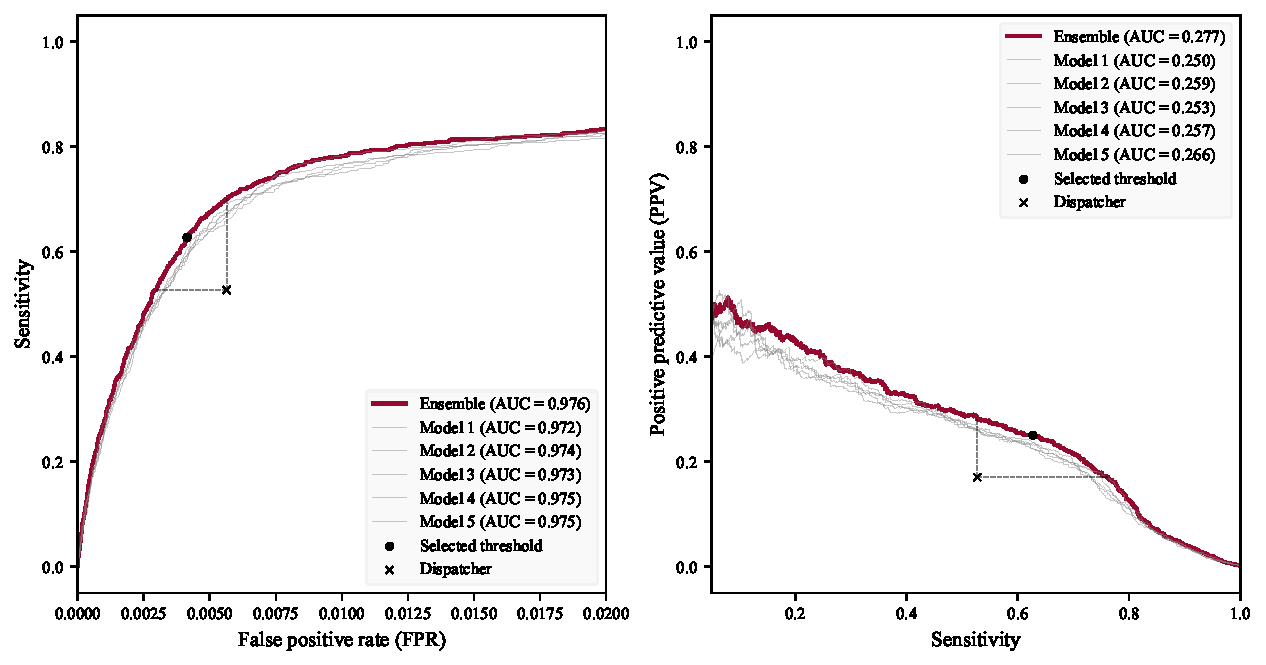
\includegraphics[width=0.95\textwidth]{paper_retrospective/figure1.pdf}
    \caption[ROC- and PPV-sensitivity curves for stroke recognition model.]{Receiver operator characteristic (ROC) curve and PPV-sensitivity curve. Left, the ROC curve and, right, PPV-sensitivity curve (precision-recall curve). Models 1-5 are the individual models that make up the ensemble model.}
    \label{fig_retrospective:figure1-roc-curve}
\end{figure}

\begin{figure}[t]
    \centering
    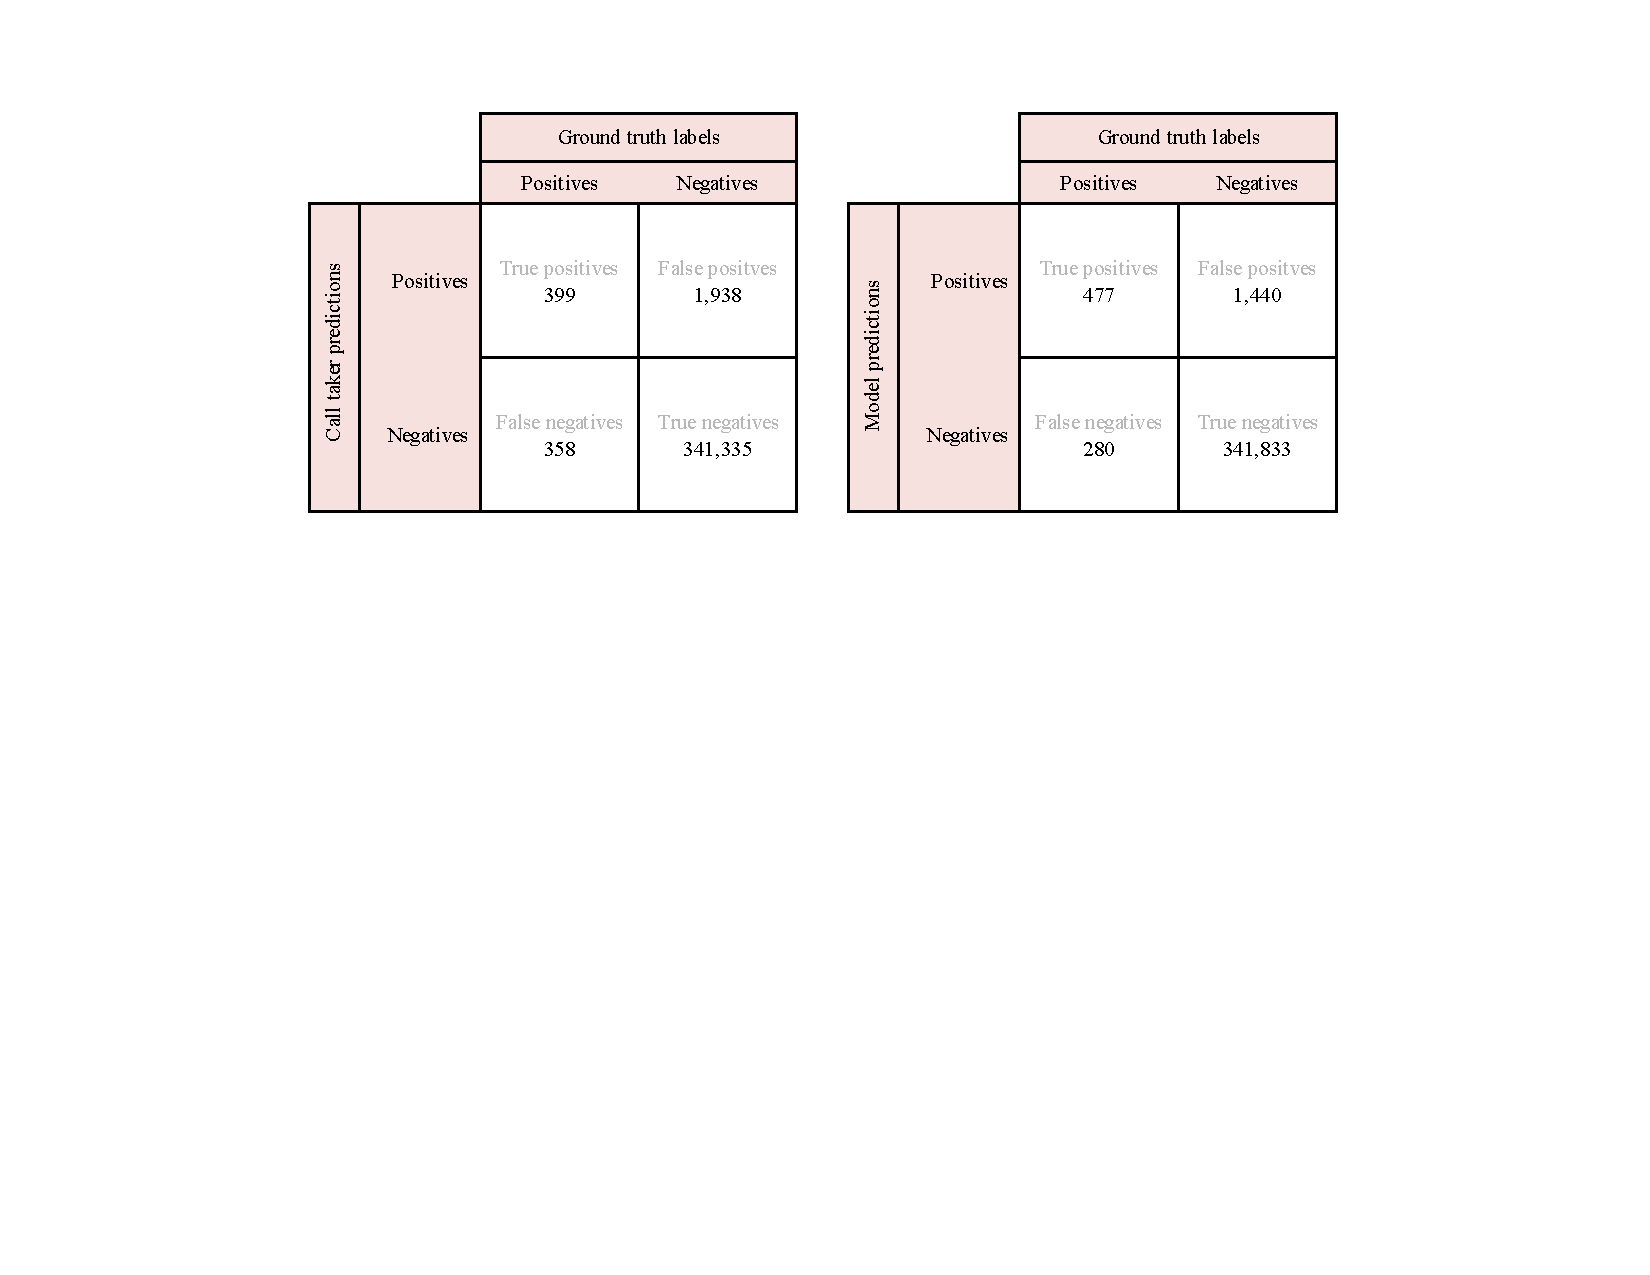
\includegraphics[width=0.98\textwidth]{paper_retrospective/figure2.pdf}
    \caption[Prediction confusion matrices for stroke recognition.]{Prediction confusion matrices. Confusion matrices of predictions for call takers and the model on the test set. Numbers for the model are given as the rounded mean over eleven runs.}
    \label{fig_retrospective:figure2-prediction-confusion-matrices}
\end{figure}


\subsection{Model explainability}

We performed an occlusion analysis to evaluate the importance of individual words for both positive and negative classifier predictions \cref{tab_retrospective:table3-occlusion-analysis}. 
Among the words with a positive rank score, several words are synonymous with stroke, such as ``blood clot", ``hemorrhagic stroke", and ``stroke". Ambulances are rarely dispatched because the MH-1813 is not intended for emergencies. Therefore, a word like ``ambulance" may also be a strong indicator of call-taker recognition, which the model has learned to mimic. Additionally, most of the remaining words can be linked to stroke-related symptoms such as ``double vision", ``difficulties speaking", and ``hangs". Particularly, words describing the side of the body where symptoms occur ranked high (such as ``left", ``right", and ``side"). Finally, some words were also related to the sudden onset of symptoms (including ``suddenly" and ``minutes").

Among the words with a negative rank score, most were strong indicators for specific conditions, symptoms, or body parts that are unrelated to stroke (such as ``tetanus", ``pregnant", ``swollen", ``fever", and ``the knee"). Another group of words used to describe aspects of treatment that are unlikely to be addressed in a stroke call included ``prescription", ``bandage", and ``OTC". Finally, a small group of words described institutions that are not commonly involved in stroke treatment (such as ``psychiatric", ``the emergency room", and ``the police").

\begin{table}[t]
    \centering
    \caption[Words with the largest positive and negative ranking score in calls predicted as stroke and non-stroke, respectively.]{English translation of words with the largest positive and negative ranking score in calls predicted as stroke and non-stroke, respectively. For this analysis, we used the model with the median F1-score out of 11 randomly seeded runs.}
    \label{tab_retrospective:table3-occlusion-analysis}
    \resizebox*{0.98\textwidth}{!}{%
    \begin{tabular}{l|lr|lr}
        \toprule
                    & \multicolumn{2}{c|}{Positive ranking score} & \multicolumn{2}{c}{Negative ranking score} \\
        \midrule
                    & \multicolumn{2}{c|}{Stroke predictions, $D=1,897$} & \multicolumn{2}{c}{Non-stroke predictions, $D=342,133$} \\
        \midrule
                    & Word, $w$ \textit{(translated)} & Occurrences, $D^{(w)}$ & Word, $w$ \textit{(translated)} & Occurrences, $D^{(w)}$ \\
        \midrule
        1.  & Ambulance & 1,680 & Tetanus & 4,378 \\        
        2.  & Blood clot & 895 & Pregnant & 8,749 \\        
        3.  & Left & 1,108 & Cut & 7,592 \\        
        4.  & Right & 1,050 & Bandage & 4,561 \\        
        5.  & Double vision & 84 & Amager (a location) & 23,776 \\        
        6.  & The words & 344 & O'clock & 94,436 \\        
        7.  & Suddenly & 783 & The emergency room & 42,809 \\        
        8.  & Arm & 709 & The police & 2,903 \\        
        9.  & Side & 1,139 & Swollen & 60,559 \\        
        10. & Stroke & 117 & Over the counter (OTC) & 4,641 \\        
        11. & Double & 113 & The neck & 30,151 \\        
        12. & Control & 134 & Fever & 112,586 \\        
        13. & Call & 39 & Prescription & 5,450 \\        
        14. & Numb & 94 & Centimeter & 12,026 \\        
        15. & Minutes & 763 & The knee & 8,875 \\        
        16. & Difficulties speaking & 44 & The pharmacy & 10,085 \\        
        17. & Hemorrhagic stroke & 133 & The stomach & 42,105 \\        
        18. & Hand & 297 & Psychiatric & 3,688 \\        
        19. & The ambulance & 521 & Pneumonia & 7,597 \\        
        20. & Slurred speech & 58 & Stomach pain & 10,551 \\        
        21. & Blood clots & 224 & Stool & 19,155 \\        
        22. & Fast & 663 & The ribs & 3,928 \\        
        23. & Express & 44 & Bleed & 10,501 \\        
        24. & Blood thinner & 259 & Bleeding & 24,313 \\        
        25. & Incoherent & 15 & Ribs & 2,941 \\        
        26. & Lopsided & 211 & Broken & 19,415 \\        
        27. & Reduced & 528 & Inflammation & 10,050 \\        
        28. & Hangs & 628 & Common cold & 8,127 \\        
        29. & Transient & 48 & Morning or morrow & 78,558 \\        
        30. & Not making sense & 14 & Swelling & 17,762 \\        
        \bottomrule
    \end{tabular}%
    }
\end{table}


\section{Discussion}

Our results showed that a machine learning framework can substantially improve stroke recognition in medical helpline calls compared to solely relying on human call-takers. This improvement was observed across all performance metrics and for basic patient demographics (age and sex). Our occlusion analysis revealed that the model relied on the relevant predictive features associated with call-taker triaging, patient symptoms, and treatment.

This study does not imply that a machine learning model can replace medical call-takers. The effectiveness of the model is fully reliant on the conversation between the call-taker and caller and the call-taker's ability to skillfully triage the patient. Instead, the model should be used as a supportive tool for call-takers in the decision-making process, contributing to a higher recognition of patients with stroke and potentially boosting the confidence of call-takers in their decisions. A similar machine learning model designed to predict cardiac arrest was tested in a randomized controlled trial (RCT) at CEMS \parencite{cite15}. The results highlighted the necessity of incorporating input from call-takers. The machine learning model for cardiac arrest has subsequently been implemented in daily practice at CEMS, in a setup similar to the one presented in our study. However, implementation of our framework requires further investigation. The relative performance gap between call-takers and the model was larger in our study than in the cardiac arrest study \parencite{cite15}, which may affect the results of a potential RCT. 

To support future work and discussions beyond the scope of this study, the supplementary material includes the results of a simulation of a live implementation where call-takers are assumed to follow a set of fixed rules based on the output of the machine learning framework \cref{app:supplementary-retrospective}. For instance, in one simulation call-takers are assumed to change any stroke negative to a positive, if the model predicts a positive. While the results of the simulation are encouraging, it is important to stress that it is not practically feasible to use a fixed rule set to overrule the call-taker. These results should only be seen as a preliminary indicator of a potential RCT. In practice, a nuanced set of guidelines should be developed over several iterations of implementation and testing.

The performance gap between the model and call-takers could be explained by the rarity of stroke calls to MH-1813 (0.250\% of all calls in 2021), which might affect call-taker awareness of stroke as a possible cause of certain symptoms. Additionally, certain stroke symptoms are so rare that some call-takers may never encounter them, increasing the risk of false negatives. The model was trained on more calls than any single call-taker would handle in a lifetime, enabling it to recognize even rare descriptors of stroke. The model is specifically trained to recognize strokes and exclusively learns from actual stroke descriptions, unlike call-takers, who are trained with generalized teaching materials to triage many different conditions. Therefore, call-takers may not have received specific training for patients with stroke and may never have encountered them. 

The model performed significantly better on men than on women. This could be attributed to several factors. First, the model may have learned to mimic call-takers with the same bias. Second, women may experience different and more challenging-to-identify symptoms than men \parencite{cite29,cite30}. Third, a higher prevalence of male patients with stroke was observed in the training data. Despite these potential sources of bias, the model exhibited less bias than call-takers did. That is, the relative performance improvements were higher for women than for men. This bias could be further reduced using advanced data augmentation and balanced data when training a machine learning model. However, such measures may degrade overall performance.

The improved sensitivity and PPV on the 65+ years group may be explained a higher prior probability of stroke for older patients and stronger evidence from the patient's medical history. The relatively high FOR and FPR for the 65+ group is likely to be a result of the much higher prevalence of stroke cases compared to the 18-64 year olds (0.85\% vs. 0.07\%). We did not have data to estimate potential bias related to race, ethnicity, language, accent, or dialects. Previous studies on speech recognition for call centers have indeed found that non-native speakers had a higher rate of transcription errors \parencite{han_deep_2017}. Since our model was trained on a representative - and therefore unbalanced - sample, we expect it to behave similarly. Future research should look to address these shortcomings, for example by utilizing self"-supervised learning on massive amounts of diverse, unlabeled data covering multiple languages, accents, and dialects.

Due to European data regulations (GDPR), it was not possible to manually transcribe MH-1813 calls to train a new speech recognition model, so we had to rely on an existing solution. This also meant that we could not evaluate the word error rate (WER) of the model. Instead, we used the downstream performance of the text classification model when trained in combination with different speech recognition models to choose the best option. Since the focus of this study is the ability to correctly recognize stroke, and not the performance of the speech recognition model alone, this approach is better suited. Indeed, the WER might be misleading when choosing a speech recognition model for a specific task. For instance, one model might fail to predict redundant minimal response words (e.g. “uh” and “uhm”) and make small inflection errors (e.g. “clot” instead of “clots”), which results in a relatively high WER, while another model only fails to predict rare, specialized words that are highly indicative of stroke (e.g. “hemorrhage” and “thrombolysis”), which results in a relatively low WER.

Although we believe that the proposed machine learning framework can be further improved, several alternatives have already been explored in the preliminary experimental phase. The speech recognition model we used was trained on 1-1-2 calls for a previous project \parencite{cite14}, and so, was specialized to a domain very similar to that of MH-1813. We also tested an open-source, multilingual model from OpenAI called Whisper \parencite{radford_robust_2023}, but found that performance degraded slightly compared to the model trained on 1-1-2. We hypothesize that this is due to Whisper's inability to handle the specific noise conditions and recognize words from a specialized medical vocabulary.

For text classification, we used an ensemble of multi-layer perceptrons (MLPs). We also tested convolutional, recurrent, and self-attention (i.e. Transformer) architectures. However, this did not improve performance. In addition, we tested a pre"=trained self"=supervised model. Although many of these models are freely available to the public, they are primarily trained on English data. Only relatively few options exist for the Danish language, none of which are specialized in the medical domain. We used a monolingual Danish BERT model, which has previously been shown to outperform a multilingual alternative from Google for Danish named entity recognition \parencite{hvingelby_dane_2020}. However, this also did not result in a significant performance improvement. We hypothesize that the number of ground truth stroke positives was too small for these advanced models to learn more complex patterns than the MLP ensemble. In addition, a self"=supervised model would likely benefit from being pre"=trained on speech or text data from the target domain. Although training such large-scale foundation models have the potential to improve the classification model further, it is beyond the scope of this study. Thus, we chose the simpler MLP ensemble. We have included references to reviews of self"=supervised learning for speech and text in the references \parencite{gururangan_don_2020,mohamed_selfsupervised_2022}. Notably, it is not uncommon for small, simple models to match or outperform large, pre"=trained models for text-classification tasks \parencite{galke_bagofwords_2022}.

This study has some limitations. First, the mapping of call recordings to electronic records was incomplete due to technical limitations in the computer-aided dispatch (CAD) registry, which limited the number of calls available to us. Of note, there was no obvious pattern of bias related to the unmapped calls, and we included all calls with matching audio files, regardless of dispatcher performance. The results could potentially be improved if more calls were available for analysis. Second, calls without a call-taker indicated diagnostic category were not included in the validation and test data because the call-taker's performance could not be evaluated. Moreover, in exploratory analyses, the model performed worse on these calls, which might be attributed to differences in population characteristics (\cref{tab_retrospective:table1-population-characteristics,tab_retrospective:table2-main-results}). Finally, the ground truth stroke labelling relied on the patient-reported time of onset being exact; however, estimating the accuracy of the timestamps in DanStroke was impossible.

In conclusion, using the largest collection of audio calls from patients with stroke to date, we developed a machine learning framework that significantly outperformed human call-takers in stroke recognition in medical helpline calls. The framework can assist human call-takers during medical helpline calls. Ideally, this would enable a higher recognition of patients with stroke in the prehospital setting, benefiting both patient outcomes and health service resource allocation.


\section{Methods}

\subsection{Data sources}

\paragraph{Copenhagen Emergency Medical Services (CEMS)}

The CEMS is responsible for providing prehospital telehealth services in the Capital Region of Denmark, with a catchment area of 1.9 million \parencite{cite17}. CEMS operates two call lines: the 1-1-2 emergency line, similar to 9-1-1 in the United States, intended for acute conditions. The other is the medical helpline 1813 (MH-1813, pronounced ``'eighteen-thirteen") intended for non- life-threatening conditions that cannot wait until a general practitioner is available \parencite{cite18}.

Call-takers for both lines, who are nurses, paramedics, or physicians, can dispatch ambulances. The condition suspected by the call-taker is categorized based on a predefined diagnostic index and stored in an electronic record using a CAD system. The CAD records are associated with the Danish civil registration number (CPR number) \parencite{cite19} of the patient. The CPR number is a unique identification assigned to all Danish residents. It is used for interactions with health services and registries, enabling cross-referencing of the data sources used in this study. The call audio is recorded and stored separately from the CAD recordings using a telephone system.

\paragraph{Danish Stroke Registry (DanStroke)}

All patients with a final diagnosis of stroke or transient ischemic attack admitted to a Danish hospital within 5 days of symptom onset are recorded in the Danish Stroke Registry \parencite{cite16}, also known as DanStroke. This record includes the patient-reported time of onset, stroke type (hemorrhagic, ischemic, or transient ischemic attack), and CPR number of the patient.
The diagnosis is obtained according to the national guidelines \parencite{baluenfeldt_national_2021}, which includes cerebral imaging and full diagnostic workup by neurologists. The validity of the Danish stroke registry has been shown to be high \parencite{wildenschild_registration_2013}, and the number of stroke mimics is therefore minimized in our dataset.


\paragraph{Inclusion and ethics}

The Danish Data Protection Agency (P-2021-475) approved this study. Danish law did not require approval from the Scientific Ethics Committee because the data were registry-based. CEMS approved the transcription of all calls made to 1-1-2 and MH-1813. All electronic records were anonymized before analysis, and the researchers did not inspect the calls manually.


\subsection{Study scope}

Stroke prevalence in calls made to the MH-1813 is lower than that in calls made to 1-1-2. Patients with stroke may exhibit different symptoms and symptom severity because MH-1813 is meant for low-acuity incidents, leading to reduced recognition. In addition, MH-1813 call-takers dispatch high-priority transport less frequently, which may affect optimal treatment timing. Therefore, we focused on MH-1813 in this study.

\subsection{Stroke dataset}

\paragraph{Cross-referencing data sources}

From the CAD medical records, we included all calls that could be matched to a corresponding audio file for 1-1-2 and MH-1813 from 2015 to 2021 for patients older than 18. The CAD records were matched with the telephone call recordings based on the call start, call duration, and call-taker identity. Due to data incompleteness, and the way the audio data is stored, at CEMS, 2,730,199 contacts could not be matched to their corresponding audio file, however, 2,361,178 contacts were successfully matched. We found no obvious pattern in the matched and unmatched calls, and we included all calls with at matching audio file. Next, a call was regarded as a case of ground truth stroke positive when the CPR number in the CAD record matched that of a DanStroke record, and the patient-reported time of onset was close to the call start time. We allowed a window of 72 hours before and 24 hours after the call starts to account for uncertainty in recording stroke onset time. We excluded calls involving subarachnoid hemorrhage cases. Finally, we considered a call to be a call-taker stroke positive when the call-taker selected the stroke diagnostic category during the call and dispatched an ambulance with the appropriate level of response \parencite{cite20}. To ensure that the effect of the machine learning framework was not overestimated, we excluded calls where diagnostic category had not been registered from the test set. We still reported the population characteristics and model performance of this group of calls to assess potential bias introduced by excluding them. A data-flow diagram is included in \cref{app:supplementary-retrospective}. The resulting dataset is the largest dataset of audio files from stroke calls collected to date. 

\paragraph{Dataset splitting}

We reserved all the MH-1813 calls from 2021 for testing. We used stratified sampling to divide the MH-1813 calls from 2015 to 2020 into validation and training subsets. The training subset was further split into five folds which were used for ensemble training. The calls were stratified based on the ground truth stroke label and the presence of a diagnostic category. Calls without diagnostic categories were only included in the training set. The 1-1-2 calls were used only for training; however, calls from 2021 were discarded to avoid temporal overlap with the test period.


\subsection{Machine learning pipeline}

We employed a two-step machine learning pipeline. First, a call was transcribed using the speech recognition model. Second, the transcript was used as input for the text classification model. The final output score was used to classify whether the call concerned a stroke. The pipeline is illustrated in \cref{app:supplementary-retrospective}.


\paragraph{Speech recognition}

The call recordings from the CEMS were stored as 8-bit linear pulse-code modulated audio, sampled at 8 kHz. A call was converted into a log-Mel spectrogram before being input into the speech recognition model. This conversion is a commonly used input representation for speech-processing tasks, which facilitates the identification of linguistic content in audio signals. We used a speech recognition model with a neural network architecture \parencite{borgholt_endtoend_2020}, consisting of two-dimensional convolutional layers \parencite{cite22} and blocks of bidirectional long short-term memory layers \parencite{hochreiter_long_1997} The output is a sequence of probability distributions over characters of the Danish alphabet, which were then converted into a human-readable transcript using a greedy decoder \parencite{graves_connectionist_2006}.


\paragraph{Text classification}

As input for the classification model, each transcript was transformed into a fixed-size bag-of-words vector, which encoded the occurrence of word and character ($n$-grams) in a fixed vocabulary. The feature selection procedure is detailed in \cref{app:supplementary-retrospective}. The model was constructed as an ensemble \parencite{hansen_neural_1990} of five identical, independently trained models. Each consists of a stack of neural network layers commonly referred to as a multi-layer perceptron \parencite{rosenblatt_perceptron_1958}. The final layer has a single scalar output and applies a sigmoid nonlinearity to produce an output score between zero and one.


\paragraph{Threshold calibration and ensembling}

For each model in the ensemble, we selected the prediction threshold as the harmonic mean of the two thresholds that respectively ensure sensitivity and PPV equal to that of the call-takers. This simplifies the comparison by ensuring a trade-off between sensitivity and PPV, similar to that of call-takers.

As the threshold differed for each model in the ensemble, computing the ensemble output score as the average output score of the individual models would not be meaningful. Instead, we first subtracted the threshold from the output score in the logit space (before sigmoid nonlinearity) for each model to obtain the same threshold (0.5). Subsequently, we defined the ensemble output score as the average of the centered output scores. The exact equations are provided in \cref{eq_retrospective:output_score,eq_retrospective:ensemble_prediction}.


\paragraph{Model training}

The speech recognition model was trained on 3,811 manually transcribed random calls (173 h) from the CEMS as part of a previous project \parencite{cite14}. These calls exclusively originated from 1- 1-2 between 2015 and 2018, ensuring no overlap with the test data used for the text classification model. The model was trained using a connectionist temporal classification objective \parencite{graves_connectionist_2006}.

We trained five models for the text classification ensemble using binary cross-entropy after transcribing all calls in the dataset using the speech recognition model. One training fold was used for early stopping using the F1-score, whereas the remaining four folds and 1-1-2 data were used for training. Thus, each model in the ensemble was trained and validated using different datasets. We ran a grid search with 96 different hyperparameter configurations and selected the ensemble model with the best F1-score for the validation set. 


\subsection{Model explainability}\label{sec_retrospective:model_explainability}

We performed an \emph{occlusion analysis} to better understand the predictions of the text classification model. This involved removing all instances of a given word from the input transcript to evaluate its impact on the model output. The word was removed before vectorization, such that all word and character $n$-grams associated with the word were discarded. Specifically, let $z^{(n, d, w)}$ be the logit output of model $n$ in the ensemble for transcript $d$ when the word $w$ is occluded. For transcript $d$, we computed the word impact score $i^{(d, w)}$ as the mean difference between the logit before and after occlusion.
%
\begin{equation}
    i^{(d,w)} = \frac{1}{N_d} \sum_{n=1}^{N_d} \left( z^{(n, d)} - z^{(n, d, w)} \right) \enspace .
\end{equation}
%
We used the logit output to compute the impact score because the difference in sigmoid-normalised output is biased towards zero for values close to 0 or 1. To select words for inspection, we computed a ranking score, $r^{(w)}$, as the sum of the signed squares of the impact:
%
\begin{equation}
    r^{(w)} = \sum_{d=1}^{N} \text{sign}\left( i^{(d, w)} \right) \left( i^{(d,w)}\right) ^2 \enspace .
\end{equation}
%
where $\text{sign}$ represents the sign function. Squaring $i^{(d,w)}$ favors rare features with a high impact over common features with a low impact.


\subsection{Statistical analysis}

We report the F1-score, sensitivity, PPV, FOR (equal to 1- negative predictive value), and FPR (equal to 1 - specificity). Due to the imbalanced nature of the dataset, the negative predictive value and specificity were greater than 99\% for all cases. We reported FOR and FPR instead because such large numerical values exhibit low relative variance, thereby obfuscating comparisons. Finally, we report the prediction confusion matrices, ROC curve, and PPV-sensitivity curve, commonly known as the precision-recall curve. All results are reported with up to three significant digits.

We present the results with and without 1-1-2 training data, subgroup analyses based on age (18–64/65+) and sex (male/female), and call-takers performance. We also report the model performance on calls without a diagnostic category from the test year 2021 to assess potential data bias. We tested our results for statistical significance using approximate permutation tests. We used one-sided paired approximate permutation tests for model-to-model and model-to-call-taker comparisons when done on the same subset. For comparisons across different subsets (e.g. male vs. female) we used one-sided independent approximate permutation tests. We computed 95\% confidence intervals (CIs) using bootstrapping \parencite{dwass_modified_1957,eden_validity_1933}. In our assessment, we accounted for random variation associated with model training by basing the means, tests, and CIs on the predictions of 11 randomly initialized training runs. Statistical significance was defined as a p-value of less than 0.05.

We used the model with the median F1-score out of the 11 runs for the occlusion analysis. We listed the 30 words with the highest positive ranking scores for calls classified as stroke and the 30 words with the highest negative ranking scores for calls classified as non-stroke.


\section*{Data availability}

The datasets used to evaluate call-taker performance and to train and evaluate the machine learning framework are legally restricted by Danish patient privacy and secrecy laws and are therefore, not publicly available. The data can be made available from the publication date but requires a Data Access Agreement, which is examined and approved by the ethics committees that approved this research.\footnote{Danish Data Protection Agency, \url{https://www.datatilsynet.dk/english}} For the same reason, the machine learning framework trained in this study is not publicly available; however, instructions on how to train it are included in the main manuscript and the supplementary material. 


\section*{Code availability}

The source code can be shared using a Creative Commons NC-ND 4.0, an international license, upon reasonable written request to the corresponding author, and requires a data use agreement. 


\section*{Acknowledgements}

We thank the staff of the CEMS for their role in generating the data used in this study. We thank Emilie Grunddal Pedersen, Mette Bjerg Lindhøj, and Jens Morten Haugård for their help and cooperation in accessing the data sources. We also thank the Centre for IT and Medical Technology (CIMT) and Corti employees Akihiro Inui and Nathaniel Joselson for their assistance in setting up and using the cloud-computing environment for training and evaluating the machine learning framework of this study. Funding for the work was received from Innovation Fund Denmark, Trygfonden, Copenhagen University Hospital - Herlev, Gentofte and University of Copenhagen. The grant providers had no role in the study design, data collection, analysis, interpretation, manuscript writing, or publication decision. Corti provided additional funds and technical expertise to develop the models. Corti was not financially compensated for this, and the project was part of its research initiatives, which were conducted in cooperation with several universities and the Innovation Fund Denmark. Corti owns the rights to the models and source code.


\section*{Author contributions}

JW, JDH and LB share lead authorship and contributed equally to the original drafting of the paper, review and editing, data curation, formal analysis, methodology, validation, and conceptualization. JDH and LB contributed to software development and funding acquisition. SNFB contributed to the conceptualization, data curation, funding acquisition, supervision, and writing - review and editing. LM contributed to conceptualization, funding acquisition, project administration, supervision, and writing - review and editing. MS contributed to supervision and writing - review and editing. HC contributed to the methodology, supervision, and writing - review and editing. CK contributed to the conceptualization, funding acquisition, methodology, project administration, supervision, and writing - review and editing. HCC contributed to the conceptualization, data curation, funding acquisition, methodology, project administration, supervision, and writing - review and editing. HCC and CK share last authorship. The three lead authors directly accessed and verified the underlying data reported in this manuscript. JW's affiliations are exclusively academic.


\section*{Competing interests}
JDH and LB received funding from the Innovation Fund Denmark. JDH and LB used Corti and hold stock warrants. LM is a co-founder, stockholder, and the Chief Technology Officer of Corti. JW received funding from Trygfonden. SNFB has no conflicts of interest to declare. HC has received funding from the Velux Foundation, Tværsfonden, Helsefonden, Hartmann Fonden, Lundbeck Foundation, and Novo Nordisk Foundation; royalties from Gyldendal; honoraria from Bayer and Bristol Meyers Squibb, and is chair of Action Plan for stroke in Europe Implementation, Co-chair of the Scientific Stroke Panel EAN and Senior Guest Editor of AHA Stroke. MS has no conflicts of interest to declare. HCC has no conflicts of interest to declare. CK received funding from the Novo Nordisk Foundation and is the chair of the Danish Resuscitation Council and vice chair of the Danish Stroke Society. Both positions are unpaid. 


}

%!TEX root = ../thesis.tex

\chapter[automated medical coding on mimic-iii and mimic-iv: a critical review and replicability study]{Automated Medical Coding on MIMIC-III and MIMIC-IV: A Critical Review and Replicability Study}
\label{chp:paper-automated}

\textit{This chapter is a piece of original research published as part of the project:} \newline
\begin{center}
    \begin{enumerate}[leftmargin=8mm,rightmargin=8mm,topsep=0mm,label={[\Alph*]}]
        \setcounter{enumi}{4}
        \item \fullcite{edin_automated_2023} \co
        \end{enumerate}
\end{center}

\ifthenelse{\equal{\skippapers}{true}}{}{


\newcommand{\lacaml}{LA$_{\textsc{caml}}$}
\newcommand{\lalaat}{LA$_{\textsc{laat}}$}


\section*{Abstract}
Medical coding is the task of assigning medical codes to clinical free-text documentation.
Healthcare professionals manually assign such codes to track patient diagnoses and treatments. Automated medical coding can considerably alleviate this administrative burden. In this paper, we reproduce, compare, and analyze state-of-the-art automated medical coding machine learning models. We show that several models underperform due to weak configurations, poorly sampled train-test splits, and insufficient evaluation. In previous work, the macro F1-score has been calculated suboptimally, and our correction doubles it. We contribute a revised model comparison using stratified sampling and identical experimental setups, including hyperparameters and decision boundary tuning. We analyze prediction errors to validate and falsify assumptions of previous works. The analysis confirms that all models struggle with rare codes, while long documents only have a negligible impact. Finally, we present the first comprehensive results on the newly released MIMIC-IV dataset using the reproduced models. We release our code, model parameters, and new MIMIC-III and MIMIC-IV training and evaluation pipelines to accommodate fair future comparisons.\footnote{\label{footnote:source_code}\url{https://github.com/JoakimEdin/medical-coding-reproducibility}}


\section{Introduction}

Medical coding is the task of assigning diagnosis and procedure codes to free-text medical documentation \parencite{dongAutomatedClinicalCoding2022,tengReviewDeepNeural2022}.
These codes ensure that patients receive the correct level of care and that healthcare providers are accurately compensated for their services. However, this is a costly manual process prone to error \parencite{tsengAdministrativeCostsAssociated2018, omalleyMeasuringDiagnosesICD2005, burnsSystematicReviewDischarge2012}.

The goal of automated medical coding (AMC) is to predict a set of codes or provide a list of codes ranked by relevance for a medical document. Numerous machine learning models have been developed for AMC \parencite{jiUnifiedReviewDeep2022, tengReviewDeepNeural2022, stanfillSystematicLiteratureReview2010}. These models are trained on datasets of medical documents, typically discharge summaries, each labeled with a set of medical codes.
While some models treat AMC as an ad-hoc information retrieval problem \parencite{rizzoICDCodeRetrieval2015,parkInformationRetrievalApproach2019}, it is more commonly posed as a multi-label classification problem \parencite{tengReviewDeepNeural2022, jiUnifiedReviewDeep2022}.

While most research in AMC has been conducted on the third version of the Medical Information Mart for Intensive Care dataset (MIMIC-III) \parencite{tengReviewDeepNeural2022, venkateshAutomatingOverburdenedClinical2023}, it remains challenging to compare the results of different models. Performance improvements are commonly attributed to model design, but differences in experimental setups make these claims hard to validate.
In addition, long documents, rare codes, and lack of training data are often cited as core research challenges \parencite{baoMedicalCodePrediction2021,dongAutomatedClinicalCoding2022,dongExplainableAutomatedCoding2021,feuchtDescriptionbasedLabelAttention2021,gaoLimitationsTransformersClinical2021,huangPLMICDAutomaticICD2022,jiDoesMagicBERT2021,jiUnifiedReviewDeep2022,kavuluruEmpiricalEvaluationSupervised2015,kimReadAttendCode2021,liICDCodingClinical2020,liuEffectiveConvolutionalAttention2021,michalopoulosICDBigBirdContextualEmbedding2022,moonsComparisonDeepLearning2020,pascualBERTbasedAutomaticICD2021,tengReviewDeepNeural2022,tengExplainablePredictionMedical2020,xieEHRCodingMultiscale2019,yangKnowledgeInjectedPrompt2022,zhangBERTXMLLargeScale2020,zhouAutomaticICDCoding2021, vuLabelAttentionModel2020, venkateshAutomatingOverburdenedClinical2023}. However, except for a few studies demonstrating performance drops on rare codes, the number of studies containing in-depth error analyses is limited \parencite{baoMedicalCodePrediction2021,dongExplainableAutomatedCoding2021,jiDoesMagicBERT2021}.

We address the above challenges. Our major contributions are:
\begin{enumerate}
    \item We reproduce the performance of state-of-the-art models on MIMIC-III. We find that evaluation methods are flawed and propose corrections that double the macro F1-scores.
    \item We find the original split of MIMIC-III to introduce strong biases in results due to missing classes in the test set. We create a new split with full class representation using stratified sampling.
    \item We perform a revised model comparison on MIMIC-III \textit{clean} using the same training, evaluation, and experimental setup for all models. We find that models previously reported as low-performing improve considerably, demonstrating the importance of hyperparameters and decision boundary tuning.
    \item We report the first results of current state-of-the-art models on the newly released MIMIC-IV dataset \parencite{johnsonMIMICIVFreelyAccessible2023, goldbergerPhysioBankPhysioToolkitPhysioNet2000}. We find that previous conclusions generalize to the new dataset.
    \item Through error analysis, we provide empirical evidence for multiple model weaknesses. Most importantly, we find that rare codes harm performance, while, in contrast to previous claims, long documents only have a negligible performance impact.
\end{enumerate}
We release our source code and new splits for MIMIC-III and IV$^\text{1}$
and hope these contributions will aid future research in AMC.


\section{Previous work}

In the following, we review datasets, model architectures, training, and evaluation of the models we compare in this study. Our criteria for selecting these models are presented in \cref{sec: inclusion and exclusion criteria}.

\subsection{Datasets}
\label{sec:dataset}
The International Classification of Diseases (ICD) is the most popular medical coding system worldwide \parencite{tengReviewDeepNeural2022}. It follows a tree-like hierarchical structure, also known as a medical ontology, to ensure the functional and structural integrity of the classification. Chapters are the highest level in the hierarchy, followed by categories, sub-categories, and codes. The World Health Organization (WHO) revises ICD periodically. Each revision introduces new codes. For instance, ICD-9 contains 18,000 codes, while ICD-10 contains 142,000.\footnote{\url{https://www.cdc.gov/nchs/icd/icd10cm_pcs_background.htm}} MIMIC-II and MIMIC-III are the most widely used open-access datasets for research on ICD coding and are provided by the Beth Israel Deaconess Medical Center \parencite{tengReviewDeepNeural2022, johnsonMIMICIIIFreelyAccessible2016, leeOpenaccessMIMICIIDatabase2011}. 
 
MIMIC-III contains medical documents annotated with ICD-9 codes collected between 2001 and 2012 \parencite{johnsonMIMICIIIFreelyAccessible2016}. Usually, discharge summaries---free-text notes on patient and hospitalization history---are the only documents used for AMC \parencite{tengReviewDeepNeural2022}. MIMIC-III \textit{full} and \textit{50} are commonly used splits. MIMIC-III \textit{full} contains all ICD-9 codes, while \textit{50} only contains the top 50 most frequent codes \parencite{mullenbachExplainablePredictionMedical2018, shiAutomatedICDCoding2018}. 

MIMIC-IV was released on January 6th, 2023, and has not previously been used for AMC. It contains data for patients admitted to the Beth Israel Deaconess Medical Center emergency department or ICU between 2008-2019  annotated with either ICD-9 or ICD-10 codes \parencite{johnsonMIMICIVFreelyAccessible2023}. The empirical frequencies of codes of each ICD version in MIMIC-IV are shown in \cref{fig:mimiciv_code_dist}.  
Statistics for the MIMIC-III \textit{50}, \textit{full}, and MIMIC-IV datasets are listed in \cref{tab:subsets}.


\begin{figure}
    \centering
    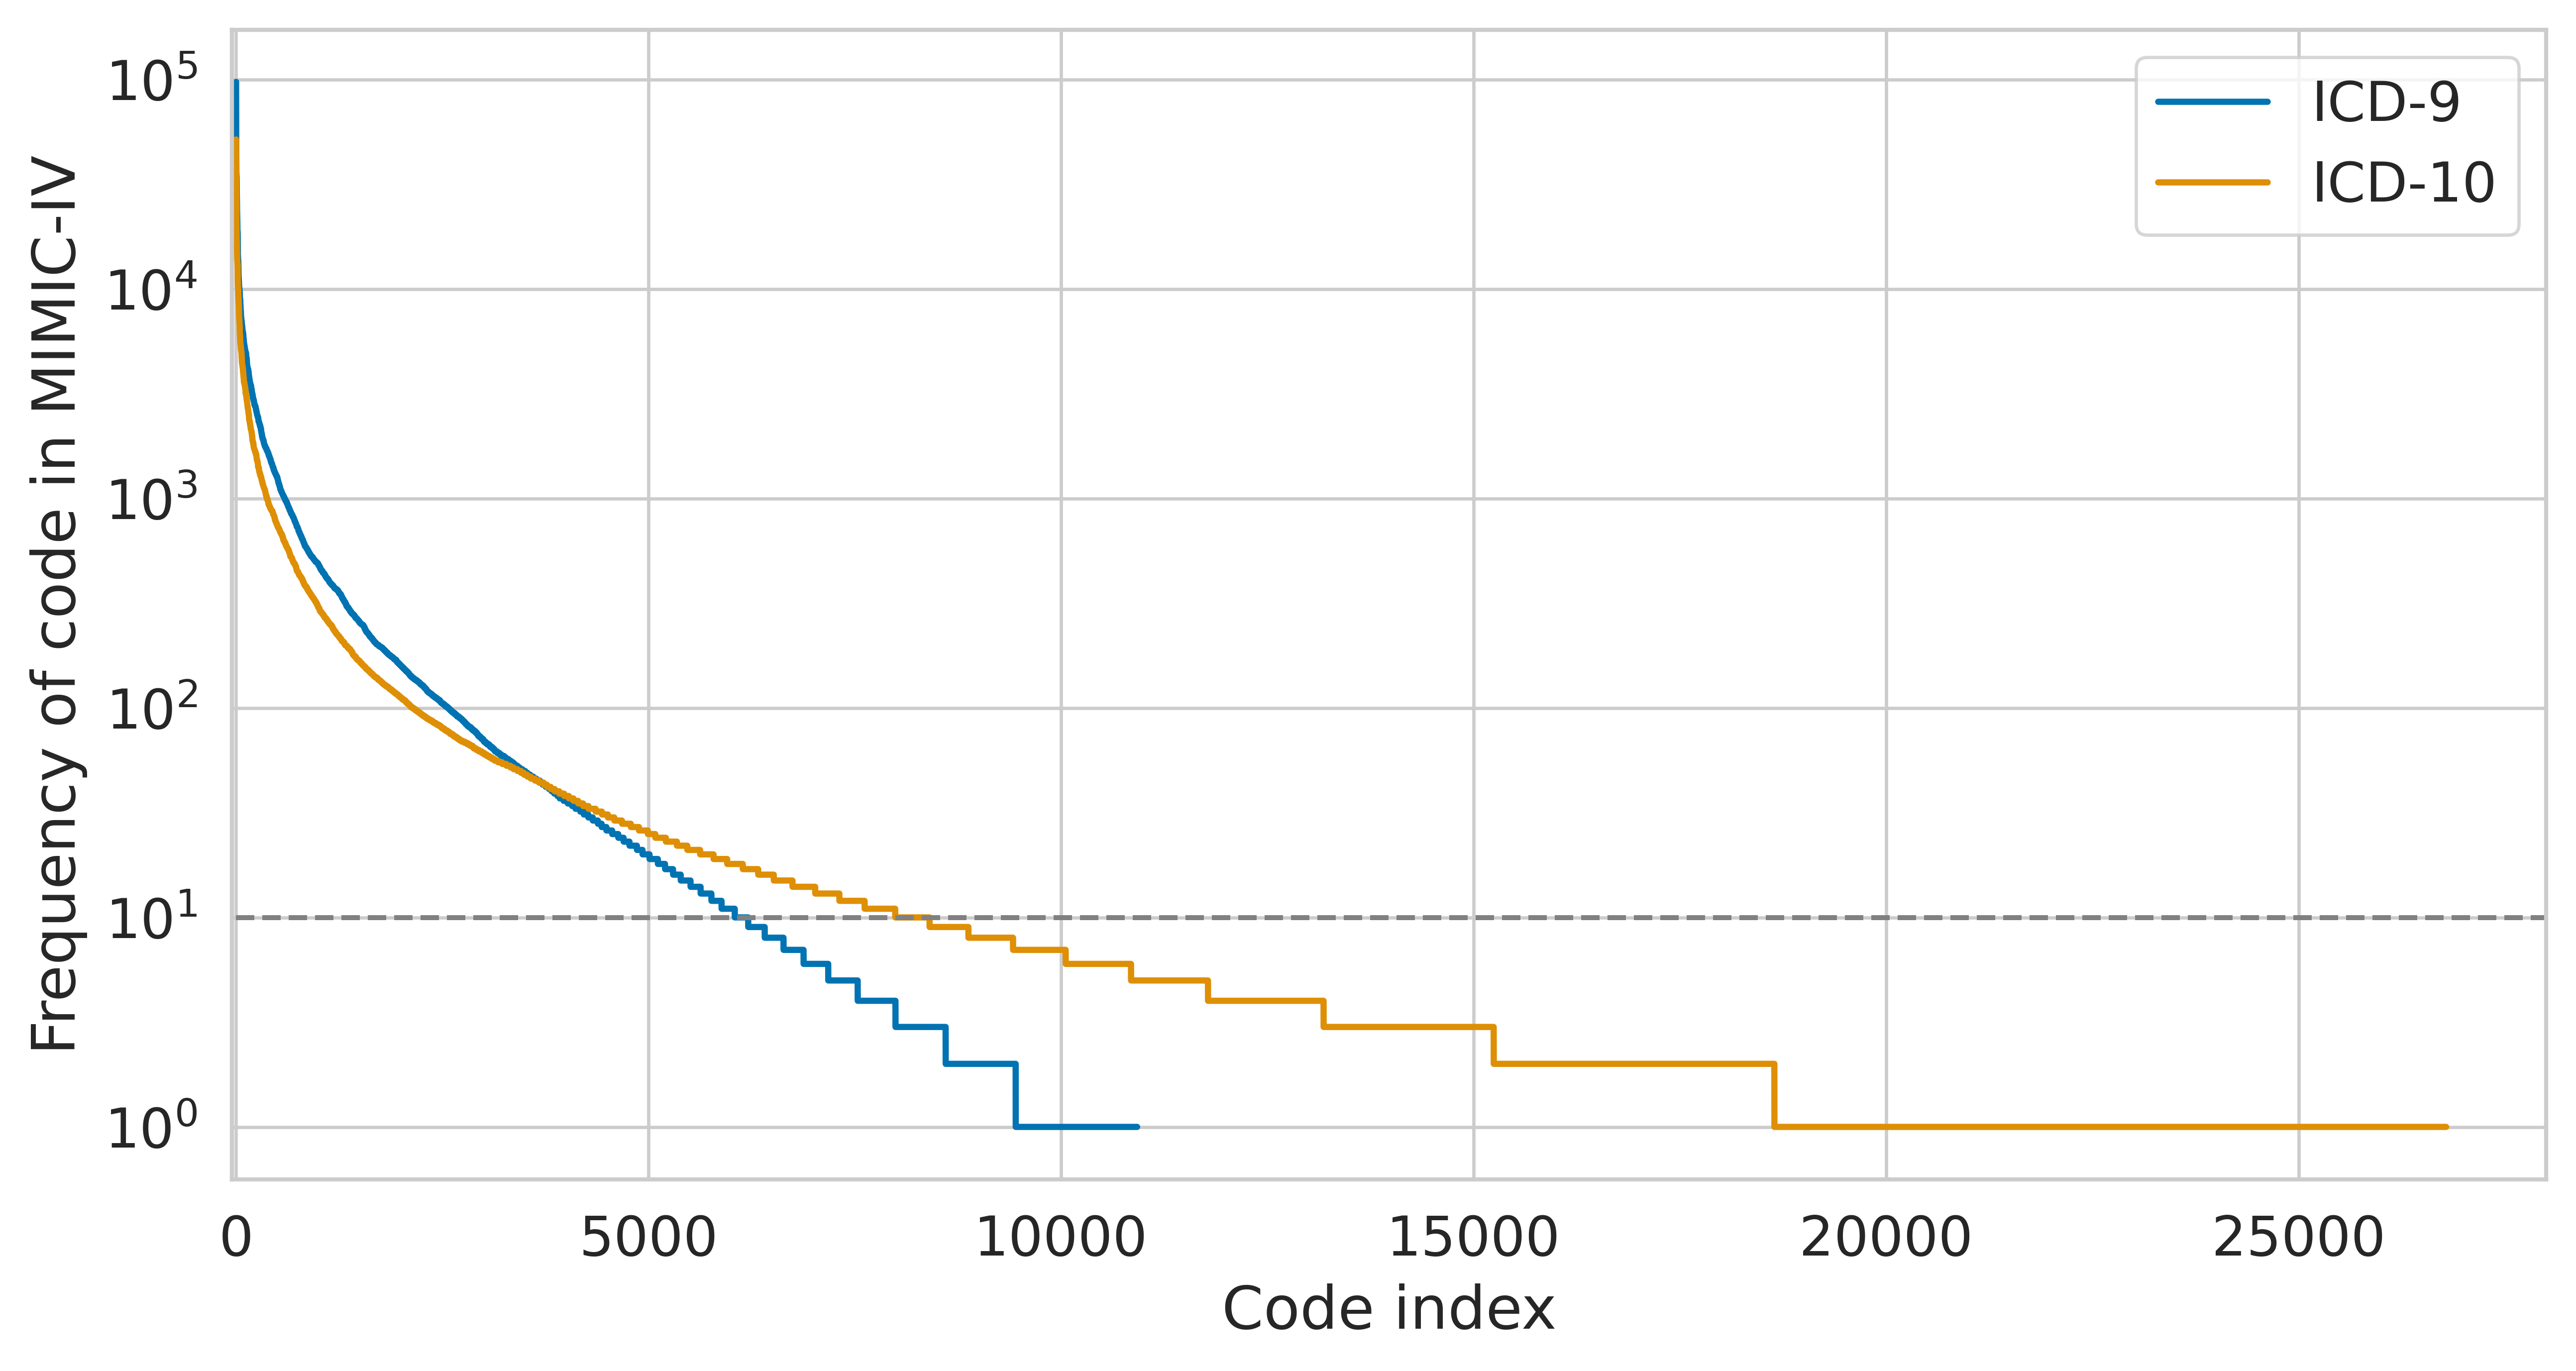
\includegraphics[width=0.9\textwidth]{paper_automated/mimiciv_code_freq.png}
    \caption[The frequency of ICD-9 and ICD-10 codes in MIMIC-IV before pre-processing.]{ The frequency of ICD-9 and ICD-10 codes in MIMIC-IV before pre-processing. As discussed in \cref{sec: splits}, we removed codes with fewer than ten instances (dashed line).}
    \label{fig:mimiciv_code_dist}
\end{figure}


\begin{sidewaystable}
    \centering
    \caption{Comparison of the previously defined MIMIC-III splits \textit{full} and \textit{50} \parencite{mullenbachExplainablePredictionMedical2018} and our proposed MIMIC-III \textit{clean} split along with similarly defined splits for MIMIC-IV \textit{ICD-9} and \textit{ICD-10} after pre-processing.}
    \label{tab:subsets}
    \resizebox*{\textwidth}{!}{%
    \begin{tabular}{lccccc}
        \toprule
        & \multicolumn{2}{c}{\textit{Previous work}} & \multicolumn{3}{c}{\textit{Our work}} \\
        \cmidrule(lr){2-3}\cmidrule(lr){4-6}
        & {MIMIC-III \textit{full}} & {MIMIC-III 50}  & {MIMIC-III \textit{clean}}  & {MIMIC-IV \textit{ICD-9}}  & {MIMIC-IV \textit{ICD-10}}\\
        \midrule
        Number of documents  & 52,723 & 11,368 &  52,712 & 209,326 & 122,279 \\
        Number of patients & 41,126 & 10,356 & 41,118 & 97,709 & 65,659 \\
        Number of unique codes  & 8,929 & 50  & 3,681 & 6,150 & 7,942\\
        Codes pr. instance: Median (IQR)    & 14 (10-20) & 5 (3-8) & 14 (10-20) & 12 (8-17) & 14 (9-20)\\
        Words pr. document: Median (IQR) & 1,375 (965-1,900) & 1,478 (1,065-1,992) & 1,311 (917-1,822) & 1,320 (997-1,715) & 1,492 (1,147-1,931)\\
        Documents: Train/val/test [\%] & 90.5/3.1/6.4 & 71.0/13.8/15.2 & 72.9/10.6/16.6  & 73.8/10.5/15.7& 72.9/10.9/16.2  \\
        Missing codes: Train/val/test [\%] & 2.7/66.4/54.3 & 0.0/0.0/0.0 & 0.0/0.1/0.0 & 0.0/0.5/0.2 & 0.0/0.5/0.1\\
        \bottomrule
    \end{tabular}%
    }
\end{sidewaystable}


\subsection{Model architectures}

Most recent state-of-the-art AMC models use an encoder-decoder architecture. The encoder takes a sequence of tokens $T \in \mathbb{Z}^{n}$ as input and outputs a sequence of hidden representations $H \in \mathbb{R}^{d_h \times n}$, where $n$ is the number of tokens in a sequence, and $d_h$ is the hidden dimension. The decoder takes $H$ as input and outputs the code probability distributions. For the task of ranking, codes are sorted by decreasing probability. For classification, code probabilities larger than a set decision boundary are predicted. 

\paragraph{Encoders:}
The encoder usually consists of pre"=trained non-contextualized word embeddings (e.g., Word2Vec) and a neural network for encoding context. More recently, pre"=trained masked language models (e.g., BERT) have gained popularity~\parencite{tengReviewDeepNeural2022}. The MIMIC-III training set or PubMed articles are commonly used for pre"=training.

\paragraph{Decoders:}
The most common decoder architectures can be grouped into three primary types. 
The simplest decoder is a pooling layer (e.g., max pooling) followed by a feed-forward neural network. More recently, label-wise attention (LA) \parencite{mullenbachExplainablePredictionMedical2018} has replaced pooling \parencite{vuLabelAttentionModel2020, liuEffectiveConvolutionalAttention2021, huangPLMICDAutomaticICD2022, liICDCodingClinical2020}. LA transforms a sequence of hidden representations $H$ into label-specific representations $V \in \mathbb{R}^{d_h \times L}$, where $L$ is the number of unique medical codes in the dataset.
It is computed as
\begin{equation}
    A = \text{softmax}(WH) \, , \quad
    V = HA^{\top} \enspace ,
\end{equation}
where the softmax normalizes each column of $WH$, $W \in \mathbb{R}^{L \times d_h}$ is an embedding matrix that learns label-specific queries, and $A \in \mathbb{R}^{L \times n}$ is the attention matrix. 
Then, $V$ is used to compute class-wise probabilities via a feedforward neural network. 
As LA was first used in the \textit{convolutional attention for multi-label classification} (CAML) model~\parencite{mullenbachExplainablePredictionMedical2018}, we refer to this method as \lacaml.

An updated label-wise attention module was introduced in the \textit{label attention model} (LAAT) \parencite{vuLabelAttentionModel2020}. We refer to this attention module as \lalaat. In \lalaat, the label-specific attention is computed similarly to  \lacaml~ as $A = \text{softmax}(UZ)$, where $U \in \mathbb{R}^{L \times d_p}$ is a learnable embedding matrix, but with 
$Z = \text{tanh}(PH)$ 
where $P \in \mathbb{R}^{d_p \times d_h}$ is a learnable matrix, $Z \in \mathbb{R}^{d_p \times n}$ and $d_p$ is a hyperparameter.


\subsection{Training and evaluation methods}\label{sec: training and evaluation methods}

\textcite{mullenbachExplainablePredictionMedical2018} released code for pre-processing the discharge summaries, generating the train-test split, and evaluating model performance on MIMIC-III which many subsequent papers have used \parencite{vuLabelAttentionModel2020, huangPLMICDAutomaticICD2022, liICDCodingClinical2020, baoMedicalCodePrediction2021, yuanCodeSynonymsMatter2022, kimReadAttendCode2021}.
Pre-processing consisted of lower-casing all text and removing words that only contain out-of-alphabet characters. Predicting procedures and diagnosis codes were treated as a single task.
The dataset was split into training, validation, and test sets using random sampling, ensuring that no patient occurred in both the training and test set. The (non-stratified) random sampling lead to 54\% of the ICD codes in MIMIC-III \textit{full} not being sampled in the test set. This complicates the interpretation of results since these codes only contribute true negatives or false positives. 
Models are evaluated using the micro and macro average of the area under the curve of the receiver operating characteristics (AUC-ROC), F1-score, and precision@k. 

While most papers use the pre-processing, train-test split, and evaluation metrics described above, they differ in several aspects of training. This may lead to performance differences unrelated to modeling choices which are undesirable when seeking to compare models. 
For instance, due to varying memory constraints of different models, documents are usually truncated to some maximum length. In the literature, this maximum varies from 2,500 to 4,000 words \parencite{mullenbachExplainablePredictionMedical2018, vuLabelAttentionModel2020, huangPLMICDAutomaticICD2022}.
Furthermore, not all papers tune the prediction decision boundary but simply set it to 0.5,
 hyperparameter search ranges and sampling methods  vary between works, and learning rate schedulers are only used in LAAT and PLM-ICD\parencite{mullenbachExplainablePredictionMedical2018, liICDCodingClinical2020}. In LAAT, the learning rate was decreased by 90\% when the F1-score had not increased for five epochs. PLM-ICD used a schedule with linear warm up followed by linear decay. 

All models except for PLM-ICD use Word2Vec embeddings pre"=trained on the MIMIC-III training set. PLM-ICD uses a BERT encoder pre"=trained on PubMed to encode the text in chunks of 128 tokens, and these contextualized embeddings are fed to a \lalaat~ layer. 

Finally, all models compute independent code probabilities using sigmoid activation functions and optimize the binary cross entropy loss function during training.
\cref{tab:model_facts} presents the selected models.


\section{Methods}

\begin{table}
    \centering
    \caption{An overview of the compared models.}
    \label{tab:model_facts}
    \begin{tabular}{llllr}
        \toprule
        Model   & Encoder & Decoder  & Param \\
        \midrule
        Bi-GRU \parencite{mullenbachExplainablePredictionMedical2018}   &  Word2Vec, Bi-GRU & Max-pool  &  9.9M\\
        CNN \parencite{mullenbachExplainablePredictionMedical2018}   & Word2Vec, CNN & Max-pool &  10.3M\\
        CAML \parencite{mullenbachExplainablePredictionMedical2018}   & Word2Vec, CNN  & \lacaml &  6.1M\\
        MultiResCNN \parencite{liICDCodingClinical2020} &  Word2Vec, ResNet & \lacaml &  11.9M\\
        LAAT \parencite{vuLabelAttentionModel2020} & Word2Vec, Bi-LSTM  & \lalaat  &  21.9M\\
        PLM-ICD \parencite{huangPLMICDAutomaticICD2022} &  BERT & \lalaat &  138.8M\\
        \bottomrule
    \end{tabular}
\end{table}

\subsection{Selection criteria}\label{sec: inclusion and exclusion criteria}

In this study, we included both models trained from scratch and models with components pre"=trained on external corpora. 
We excluded models that use multi-modal inputs, such as medical code descriptions \parencite{kimReadAttendCode2021, mullenbachExplainablePredictionMedical2018, vuLabelAttentionModel2020, caoHyperCoreHyperbolicCograph2020, baoMedicalCodePrediction2021}, code synonyms \parencite{yuanCodeSynonymsMatter2022}, code hierarchies \parencite{caoHyperCoreHyperbolicCograph2020, xieEHRCodingMultiscale2019}, or associated Wikipedia articles \parencite{baiImprovingMedicalCode2019}, because they introduced additional complexity without providing evidence for significant performance improvements \parencite{mullenbachExplainablePredictionMedical2018, vuLabelAttentionModel2020, tengReviewDeepNeural2022}. We excluded works without publically available source code as the experiment descriptions often lacked important implementation details.

\subsection{Evaluation metrics}
\label{sec:metrics}
Similar to previous work, we evaluated models using AUC-ROC, F1-score, and precision@$k$. Additionally, we introduced exact match ratio (EMR), R-precision, and mean average precision (MAP). The EMR is the percentage of instances where all codes were predicted correctly. This allowed us to measure how many documents were predicted perfectly, which is important for \textit{fully automated} medical coding.
Where precision@$k$ is computed based on the top-$k$ codes (i.e., $k$ is fixed), R-precision considers a number of codes equal to the true number of relevant codes. Thus, R-precision is useful when the number of relevant codes varies considerably between documents, which is the case for the MIMIC datasets. Finally, in contrast to all other metrics, MAP considers the exact rank of all relevant codes in a document.


\begin{sidewaystable}
    \centering
    \caption[Hyperparameters, maximum document lengths, and decision boundary tuning strategies used in the original works compared to improved settings.]{ Hyperparameters, maximum document lengths, and decision boundary tuning strategies used in the original works compared to the optimal settings found in this paper (marked with *). LR is the learning rate scheduler. ``Length" is the maximum number of words a document can contain before being truncated. $\dagger$ applies to models using word-piece tokenization. These models were filtered on the number of sub-words instead of full words. ``DB tune" is whether the optimal decision boundary was found using the validation set. If a paper did not tune the decision boundary, it was set to 0.5.}
    \label{tab:hyperparameters}
    \resizebox*{\textwidth}{!}{%
    \begin{tabular}{lccccccccc}
        \toprule
        & \multicolumn{7}{c}{Hyperparameters} & & \\
        \cmidrule(lr){2-8}
        Model & Batch Size & Weight Decay & Learning Rate & Dropout & LR Scheduler & Optimizer & Epochs & Length & DB tune \\
        \midrule
        Bi-GRU  & 16 &  0.0 & 0.003 &  0.2   & no  & Adam &  100 & 2500 & no\\
        Bi-GRU$^*$  & 8 &  0.0001 & 0.001 &  0   & yes  & AdamW &  20 & 4000 & yes\\
        \hline
        CNN  & 16 &  0.0 & 0.003  &  0.2 & no  & Adam &  100 & 2500 & no\\
        CNN$^*$    & 8 &  0.00001 & 0.001  &  0 & yes  & AdamW &  20 & 4000 & yes \\
        \hline
        CAML  & 16 &  0.0 & 0.0001  &  0.2  & no  & Adam  &  200 & 2500 & no\\
        CAML$^*$    & 8 &  0.001 & 0.005  &  0.2  & yes  & AdamW  &  20 & 4000 & yes\\
        \hline
        MultiResCNN & 16 &  0.0 & 0.0001  &  0.2  & no  & Adam &  200 & 2500 & no\\
        MultiResCNN$^*$  & 16 &  0.0001 & 0.0005  &  0.2  & yes  & AdamW &  20 & 4000 & yes\\
        \hline
        LAAT   & 8 &  0.0 & 0.0001  &  0.3  & yes  & AdamW &  50 & 4000 & no\\
        LAAT$^*$    & 8 &  0.001 & 0.001  &  0.2  & yes  & AdamW &  20 & 4000 & yes\\
        \hline
        PLM-ICD  & 8 &  0.0 & 0.00005  &  0.2  & yes  & AdamW &  20 & 3072$^\dagger$ & yes \\
        PLM-ICD$^*$   & 16 &  0.0 & 0.00005  &  0.2  & yes  & AdamW &  20 & 4000 & yes \\
        \bottomrule
    \end{tabular}%
    }
\end{sidewaystable}


Previous works calculated the macro F1-score as the harmonic mean of the macro precision and macro recall \parencite{mullenbachExplainablePredictionMedical2018, liICDCodingClinical2020, vuLabelAttentionModel2020, huangPLMICDAutomaticICD2022}. \textcite{opitzMacroF1Macro2021} analyze macro F1 formulas common in multi-class and multi-label classification. They demonstrate that the above formulation is suboptimal, as it rewards heavily biased classifiers in unbalanced datasets. Therefore, as recommended by the authors, we calculated the macro F1-score as the arithmetic mean of the F1-score for each class.
As seen in \cref{tab:subsets}, 54\% of codes in MIMIC-III \textit{full} are missing in the test set. Previous works set the F1-score of all the missing codes in the test set to 0, resulting in a misleadingly low macro F1-score. Because 54\% of the codes are missing, the maximum possible macro F1-score is 46\%. 
We ignored all codes not in the test set for our reproduction, essentially trading bias for variance. 
For our revised comparison, we resolved the issue by instead sampling new splits that reduce missing codes to a negligible fraction (see \cref{sec: splits}) and ignoring the few that were still missing.


\subsection{Definition of splits}
\label{sec: splits}

% \cref{tab:subsets}

We define three new splits: MIMIC-III \textit{clean}, MIMIC-IV \textit{ICD-9}, and \textit{ICD-10}.
As described in \cref{sec:metrics}, 54\% of the codes in MIMIC-III \textit{full} are absent from the test set, which introduces significant bias in the model evaluation metrics. Therefore, we created a new MIMIC-III split to ensure that most codes are present in both the training and test set. 
Specifically, we removed codes with fewer than ten occurrences, doubled the test set size, and sampled the documents using multi-label stratified sampling \parencite{sechidisStratificationMultilabelData2011}. 
We ensured that no patient occurred in both the training and test set, preprocessed the text, and considered procedures and diagnosis codes as a single task as done by \textcite{mullenbachExplainablePredictionMedical2018}.
We based our new split on the v1.4 version of the dataset and refer to it as MIMIC-III \textit{clean}.
Using the same method, we created two splits for MIMIC-IV v2.2: one containing all documents labeled with ICD-9 codes and one with ICD-10 codes.


\subsection{Reproducibility experiments}

We ran reproducibility experiments with all models to evaluate whether the results in the original works could be reproduced and to validate our reimplementations. We ran these experiments on MIMIC-III \textit{full}, and \textit{50} as in the original works \parencite{mullenbachExplainablePredictionMedical2018,liICDCodingClinical2020,vuLabelAttentionModel2020,huangPLMICDAutomaticICD2022}. We used the hyperparameters reported in each paper (see \cref{tab:hyperparameters}) and report both the original and the revised macro F1-scores discussed in \cref{sec:metrics}.

\subsection{Revised comparison}
To address the issues associated with comparing results reported by previous works described in \cref{sec: training and evaluation methods,sec:metrics}, we perform a revised model comparison. We run experiments on the new MIMIC-III \textit{clean}, MIMIC-IV \textit{ICD-9}, and \textit{ICD-10}.
All models were trained for 20 epochs using a learning rate schedule with linear warm up for the first 2K updates followed by linear decay \parencite{huangPLMICDAutomaticICD2022}. We found this schedule to speed up the training convergence of all the models.
Whereas original works use Adam or AdamW, we used AdamW for all experiments as it corrects the weight decay implementation of Adam \parencite{kingmaAdamMethodStochastic2017, loshchilovDecoupledWeightDecay2022}. For each model, we tuned the decision boundary to maximize the micro F1-score on the validation set. We used randomized sampling to find optimal settings for dropout, weight decay, learning rate, and batch size. The hyperparameter search was performed on MIMIC-III \textit{clean}, and the MIMIC-IV splits. We found that the best setting for each model generalized across datasets. Using this setting, we ran each model ten times with different seeds on each dataset. All documents were truncated to a maximum of 4000 words. The hyperparameters, maximum document lengths, and decision boundary tuning strategy are summarized in \cref{tab:hyperparameters}. 

We performed an ablation study to analyze which changes had the largest impact on performance. 
Specifically, we evaluated the effect of truncation, hyperparameter search, and decision boundary tuning. We modified one of these at a time: We ran one experiment where documents were truncated to a maximum length of 2,500 words, a second experiment where the models were trained with the hyperparameters, number of epochs, and learning rate schedule used in the original works, and a third experiment where the decision boundary was set to 0.5 instead of tuned.

\subsection{Error analysis}
To validate and falsify the commonly cited challenges of AMC, which include a lack of training data, long documents, and rare codes, we performed an error analysis. In addition to analyzing rare codes, we contribute an in-depth code analysis aiming to identify the attributes that make certain codes challenging to predict.


\paragraph{Amount of training data:}
Multiple studies attribute poor performance to data sparsity of MIMIC-III, which contains only fifty thousand examples \parencite{kavuluruEmpiricalEvaluationSupervised2015,tengExplainablePredictionMedical2020,yanMedicalCodingClassification2010,yangKnowledgeInjectedPrompt2022}. MIMIC-IV \textit{ICD-9} contains four times as many examples, which allows analyzing the effect of training set size. We train each model on 25k, 50k, 75k, 100k, and 125k examples and report micro and macro F1 on the fixed test set. The training subsets were sampled from the training set using multi-label stratified sampling to ensure the same code distributions \parencite{sechidisStratificationMultilabelData2011}.

\paragraph{Document length:}
We analyzed whether model performance correlates with document length on MIMIC-IV \textit{ICD-9}. Specifically, we calculated the Pearson and Spearman correlation between the number of words in the documents and the micro F1-score for all models. For each model, we used the best seed from the revised comparison.

\paragraph{Code analysis:}
To analyze the performance impact of rare codes, we first calculated the Pearson and Spearman correlation between model performance on each code and the corresponding code frequency in the training data. We calculated these correlations for all splits. To identify attributes of challenging codes, we analyzed model performance on the chapter level of the ICD-10 classification system. Using high-level chapters instead of codes allows us to group examples into categories, which we use as a starting point for further analysis. We limit the scope of the analysis to diagnosis codes. We focused on ICD-10 because it is the classification system currently in use at most hospitals. 


\begin{sidewaystable}
    \centering
    \caption[Reproduced test set results compared with those from the original works.]{ Reproduced test set results compared with those from the original works. Our reproduced results are indicated with *. The results were reproduced on MIMIC-III v1.4 with the preprocessing pipeline and splits of \textcite{mullenbachExplainablePredictionMedical2018}. Each model was reproduced using the hyperparameters presented in the respective paper. We use both macro F1 formulas: Macro$^\dagger$ refers to the method used in the original work, while Macro refers to the corrected version used in this paper.}
    \label{tab:reproduced_results}
    \resizebox*{\textwidth}{!}{%
    \begin{tabular}{l  cc  ccc  cc  cc  ccc  c}
        \toprule
        & \multicolumn{7}{c}{MIMIC-III \textit{full}} & \multicolumn{6}{c}{MIMIC-III \textit{50}} \\
        \cmidrule(lr){2-8}\cmidrule(lr){9-14}
        & \multicolumn{2}{c}{AUC-ROC} & \multicolumn{3}{c}{F1} & \multicolumn{2}{c}{Precision@$k$}  & \multicolumn{2}{c}{AUC-ROC} & \multicolumn{3}{c}{F1} & Precision@$k$  \\
        & Micro & Macro & Micro & Macro$^\dagger$ & Macro & 8 & 15 & Micro & Macro & Micro & Macro$^\dagger$ & Macro & 5 \\
        \midrule
        CNN &  96.9 & 80.6 &  41.9& 4.2 & -& 58.1 &  48.8  & 90.7 & 87.6 & 62.5 & 57.6 & - & 62.0  \\
        CNN$^*$ & 97.3 & 83.1 & 41.5 & 3.4 & 6.7 & 61.9 & 47.2 & 91.9 & 89.2 & 64.9 & 58.8 & 58.0 &  62.6 \\
        \hline
        Bi-GRU & 97.1 & 82.2 & 41.7 & 3.8 & - & 58.5 & 44.5  &  89.2 & 82.8 & 54.9 &  48.4 & - &  59.1  \\
        Bi-GRU$^*$  & 98.0 & 87.1 & 42.6 & 3.6 & 7.0 & 65.0 & 49.8 & 89.3 & 85.2 & 56.1 & 46.2 & 43.1 & 57.9  \\
        \hline
        CAML  &  98.6 &  89.5 &  53.9 & 8.8 & - &  70.9 &  56.1  & 90.9 & 87.5 &  61.4 &  53.2 & - &   60.9  \\
        CAML$^*$ & 98.4 & 88.4 & 49.5 & 5.6 & 11.3 & 69.9 & 54.9 & 91.1 & 87.5 & 60.6 & 52.4 & 51.0 & 61.1  \\
        \hline
        MultiResCNN  &  98.6 &  91.0 & 55.2 & 8.6 & - & 73.4 & 58.4  &  93.8 &  89.9 &  67.0 &  60.6 & - &  64.1 \\
        MultiResCNN$^*$  & 98.6 & 90.8 & 56.5 & 9.2 & 18.5 & 73.4 & 58.4 & 92.4 & 89.7 & 67.3 & 62.2 & 61.1 & 63.4  \\
        \hline
        LAAT  &  98.8 &  91.9 &  57.5 & 9.9 & - &  74.5 &  59.1  &  94.6 &  92.5 &  71.5 &  66.6 & - &  67.5 \\
        LAAT$^*$ & 98.6 & 89.5 & 56.1 & 8.2 & 16.2 & 73.9 & 58.7 & 92.8 & 90.5 & 66.8 & 60.8 & 59.2 & 64.0  \\
        \hline
        PLM-ICD  &  98.9 & 92.6 &  59.8 & 10.4 & - &  77.1 &  61.3  & - & - & - & - & - & -  \\
        PLM-ICD$^*$ & 98.8 & 92.3 & 58.9 & 11.1 & 22.8 & 75.7 & 60.5 & 93.8 & 91.7 & 70.5 & 66.3 & 65.4 & 65.7 \\
        \bottomrule
    \end{tabular}%
    }
\end{sidewaystable}

\section{Results}
\subsection{Reproduced results}


In \cref{tab:reproduced_results}, we report the reproduced results on MIMIC-III \textit{full} and \textit{50} using hyperparameters as reported in the original papers. We list the original and corrected macro F1-score described in \cref{sec:metrics}. In most cases, our corrections doubled the macro F1-scores on MIMIC-III \textit{full}. The differences were smaller on MIMIC-III \textit{50} because all included codes are in the test set.


\subsection{Revised comparison}

\begin{sidewaystable}
    \centering
    \caption[Results on the MIMIC-III \textit{clean}, MIMIC-IV \textit{ICD-9} and MIMIC-IV  \textit{ICD-10} test sets presented as percentages.]{ Results on the MIMIC-III \textit{clean}, MIMIC-IV \textit{ICD-9} and MIMIC-IV  \textit{ICD-10} test sets presented as percentages. Micro F1-scores rank the table in ascending order. Each model was trained ten times with different seeds. We performed a McNemar's test with Bonferroni correction and found that all the models are significantly different ($p < 0.001$).}
    \label{tab:fair_results}
    \resizebox*{\textwidth}{!}{%
    \begin{tabular}{llccccccccc}
        \toprule
        & & \multicolumn{5}{c}{Classification} & \multicolumn{4}{c}{Ranking} \\ 
        \cmidrule(lr){3-7}\cmidrule(lr){8-11}
         & & \multicolumn{2}{c}{AUC-ROC} & \multicolumn{2}{c}{F1} & EMR & \multicolumn{2}{c}{Precision@k} & R-precision & MAP \\
         & & Micro & Macro & Micro & Macro &  & 8 & 15 &  &  \\
        \midrule
        \multirow{6}{*}{\shortstack[c]{MIMIC-III \\ clean}} & CNN & 97.1$\pm$0.0 & 88.1$\pm$0.2 & 48.0$\pm$0.3 & 9.9$\pm$0.4 & 0.1$\pm$0.0 & 61.6$\pm$0.2 & 46.6$\pm$0.1 & 49.1$\pm$0.2 & 50.6$\pm$0.2 \\
        & Bi-GRU  & 97.8$\pm$0.1 & 91.1$\pm$0.2 & 49.7$\pm$0.4 & 12.2$\pm$0.2 & 0.1$\pm$0.0 & 62.8$\pm$0.4 & 47.6$\pm$0.4 & 50.1$\pm$0.4 & 52.1$\pm$0.4 \\
        & CAML & 98.2$\pm$0.0 & 91.4$\pm$0.2 & 55.4$\pm$0.1 & 20.4$\pm$0.3 & 0.1$\pm$0.0 & 67.7$\pm$0.2 & 52.8$\pm$0.1 & 55.8$\pm$0.1 & 58.9$\pm$0.2 \\
        & MultiResCNN & 98.5$\pm$0.0 & 93.1$\pm$0.3 & 56.4$\pm$0.2 & 22.9$\pm$0.6 & 0.1$\pm$0.0 & 68.5$\pm$0.2 & 53.5$\pm$0.1 & 56.7$\pm$0.2 & 59.9$\pm$0.3 \\
        & LAAT & 98.6$\pm$0.1 & 94.0$\pm$0.3 & 57.8$\pm$0.2 & 22.6$\pm$0.6 & 0.2$\pm$0.1 & 70.1$\pm$0.2 & 54.8$\pm$0.2 & 58.0$\pm$0.2 & 61.7$\pm$0.3 \\
        & PLM-ICD & \bfseries 98.9$\pm$0.0 & \bfseries 95.9$\pm$0.1 & \bfseries 59.6$\pm$0.2 & \bfseries 26.6$\pm$0.8 & \bfseries 0.4$\pm$0.0 & \bfseries 72.1$\pm$0.2 & \bfseries 56.5$\pm$0.1 & \bfseries 60.1$\pm$0.1 & \bfseries 64.6$\pm$0.2 \\
        \hline
        \multirow{6}{*}{\shortstack[c]{MIMIC-IV \\ ICD-9}} & CNN  & 98.1$\pm$0.1 & 89.4$\pm$0.5 & 52.4$\pm$0.1 & 12.6$\pm$0.4 & 0.6$\pm$0.0 & 61.3$\pm$0.1 & 45.6$\pm$0.0 & 52.9$\pm$0.1 & 55.2$\pm$0.1 \\
        & Bi-GRU  & 98.8$\pm$0.0 & 93.8$\pm$0.1 & 55.5$\pm$0.1 & 16.6$\pm$0.2 & 0.7$\pm$0.0 & 64.1$\pm$0.1 & 47.8$\pm$0.1 & 55.8$\pm$0.1 & 58.9$\pm$0.1 \\
        & CAML & 98.8$\pm$0.0 & 90.7$\pm$0.3 & 58.6$\pm$0.1 & 19.3$\pm$0.1 & 0.6$\pm$0.0 & 66.3$\pm$0.1 & 50.3$\pm$0.0 & 58.5$\pm$0.1 & 62.4$\pm$0.1 \\
        & MultiResCNN  & 99.2$\pm$0.0 & 95.1$\pm$0.1 & 60.4$\pm$0.0 & 27.7$\pm$0.3 & 0.8$\pm$0.0 & 67.6$\pm$0.0 & 51.8$\pm$0.0 & 60.4$\pm$0.0 & 64.7$\pm$0.1 \\
        & LAAT  & 99.3$\pm$0.0 & 96.0$\pm$0.3 & 61.7$\pm$0.1 & 26.4$\pm$0.9 & 0.9$\pm$0.0 & 68.9$\pm$0.1 & 52.7$\pm$0.1 & 61.7$\pm$0.2 & 66.3$\pm$0.2 \\
        & PLM-ICD  & \bfseries 99.4$\pm$0.0 & \bfseries 97.2$\pm$0.2 & \bfseries 62.6$\pm$0.3 & \bfseries 29.8$\pm$1.0 & \bfseries 1.0$\pm$0.1 & \bfseries 70.0$\pm$0.2 & \bfseries 53.5$\pm$0.2 & \bfseries 62.7$\pm$0.3 & \bfseries 68.0$\pm$0.3 \\
        \hline
        \multirow{6}{*}{\shortstack[c]{MIMIC-IV \\ ICD-10}} & CNN & 97.5$\pm$0.1 & 87.9$\pm$0.4 & 47.2$\pm$0.6 & 8.0$\pm$0.4 & 0.3$\pm$0.0 & 60.3$\pm$0.1 & 45.7$\pm$0.1 & 47.3$\pm$0.2 & 48.2$\pm$0.2 \\
        & Bi-GRU  & 98.3$\pm$0.0 & 92.4$\pm$0.2 & 50.1$\pm$0.2 & 10.6$\pm$0.4 & 0.3$\pm$0.0 & 62.6$\pm$0.2 & 47.7$\pm$0.2 & 49.6$\pm$0.1 & 51.1$\pm$0.2 \\
        & CAML  & 98.5$\pm$0.0 & 91.1$\pm$0.1 & 55.4$\pm$0.2 & 16.0$\pm$0.3 & 0.3$\pm$0.0 & 66.8$\pm$0.2 & 52.2$\pm$0.1 & 54.5$\pm$0.2 & 57.4$\pm$0.2 \\
        & MultiResCNN  & 99.0$\pm$0.0 & 94.5$\pm$0.2 & 56.9$\pm$0.1 & \bfseries 21.1$\pm$0.2 & \bfseries 0.4$\pm$0.0 & 67.8$\pm$0.1 & 53.5$\pm$0.1 & 56.1$\pm$0.1 & 59.3$\pm$0.2 \\
        & LAAT  & 99.0$\pm$0.1 & 95.4$\pm$0.3 & 57.9$\pm$0.1 & 20.3$\pm$0.4 & \bfseries 0.4$\pm$0.0 & 68.9$\pm$0.1 & 54.3$\pm$0.1 & 57.2$\pm$0.1 & 60.6$\pm$0.2 \\
        & PLM-ICD   & \bfseries 99.2$\pm$0.0 & \bfseries 96.6$\pm$0.2 & \bfseries 58.5$\pm$0.7 & \bfseries 21.1$\pm$2.3 & \bfseries 0.4$\pm$0.0 & \bfseries 69.9$\pm$0.6 & \bfseries 55.0$\pm$0.6 & \bfseries 57.9$\pm$0.8 & \bfseries 61.9$\pm$0.9 \\
        
        \bottomrule
    \end{tabular}%
    }
\end{sidewaystable}

The results of our revised comparison on MIMIC-III \textit{clean}, MIMIC-IV \textit{ICD-9}, and \textit{ICD-10} are shown in \cref{tab:fair_results}. Contrary to the originally reported results, Bi-GRU performs better than CNN in all metrics. Otherwise, the model performance ranking is unchanged from the original works. PLM-ICD outperformed the other models on all metrics and all datasets. The models previously reported as least performant improved the most. 

The ablation study results are shown in \cref{tab:ablation_study} for MIMIC-III \textit{clean}. Truncating the documents to 2,500 words instead of 4,000 had little impact on the performance. Using the hyperparameters from the original works degraded the performance substantially for CAML, Bi-GRU, and CNN but had a smaller effect on the other models. Not tuning the decision boundary had the largest negative effect on all models except MultiResCNN. In \cref{fig:threshold_tuning}, we plot the relationship between the decision boundary and F1-scores. LAAT and MultiResCNN perform similarly when using a decision boundary of 0.5. However, when tuning the decision boundary, LAAT outperforms MultiResCNN considerably.
Similar results were obtained on the other datasets. 

\begin{sidewaystable}
    \centering
    \caption[Ablation study on MIMIC-III \textit{clean}.]{ Ablation study on MIMIC-III \textit{clean}. The numbers are the micro/macro F1-scores on the test set.}
    \label{tab:ablation_study}
    \resizebox*{\textwidth}{!}{%
    \begin{tabular}{lcccccc}
        \toprule
         & PLM-ICD & LAAT & MultiResCNN & CAML & Bi-GRU & CNN \\
        \midrule
        Our result & 59.6/26.6 & 57.8/22.6 & 56.4/22.9 & 55.4/20.4 & 49.7/12.2 & 48.0/9.9 \\
        \hline
        Input length truncated at 2500 words & 59.4/26.2 & 57.6/22.3 & 56.0/23.2 & 54.8/19.7 & 49.4/12.0 & 47.9/9.8 \\
        No decision boundary tuning & 58.7/23.0 & 56.2/19.0 & 56.2/22.6 & 53.3/17.1 & 45.3/8.1 & 43.8/7.0 \\
        Original hyperparameters & 59.6/27.0 & 57.5/21.6 & 56.4/20.0 & 52.8/17.3 & 48.1/11.2 & 46.9/10.2 \\
        \bottomrule
        \end{tabular}%
    }
\end{sidewaystable}


\begin{figure}
    \centering
    \begin{subfigure}[b]{0.9\textwidth}
        \centering
        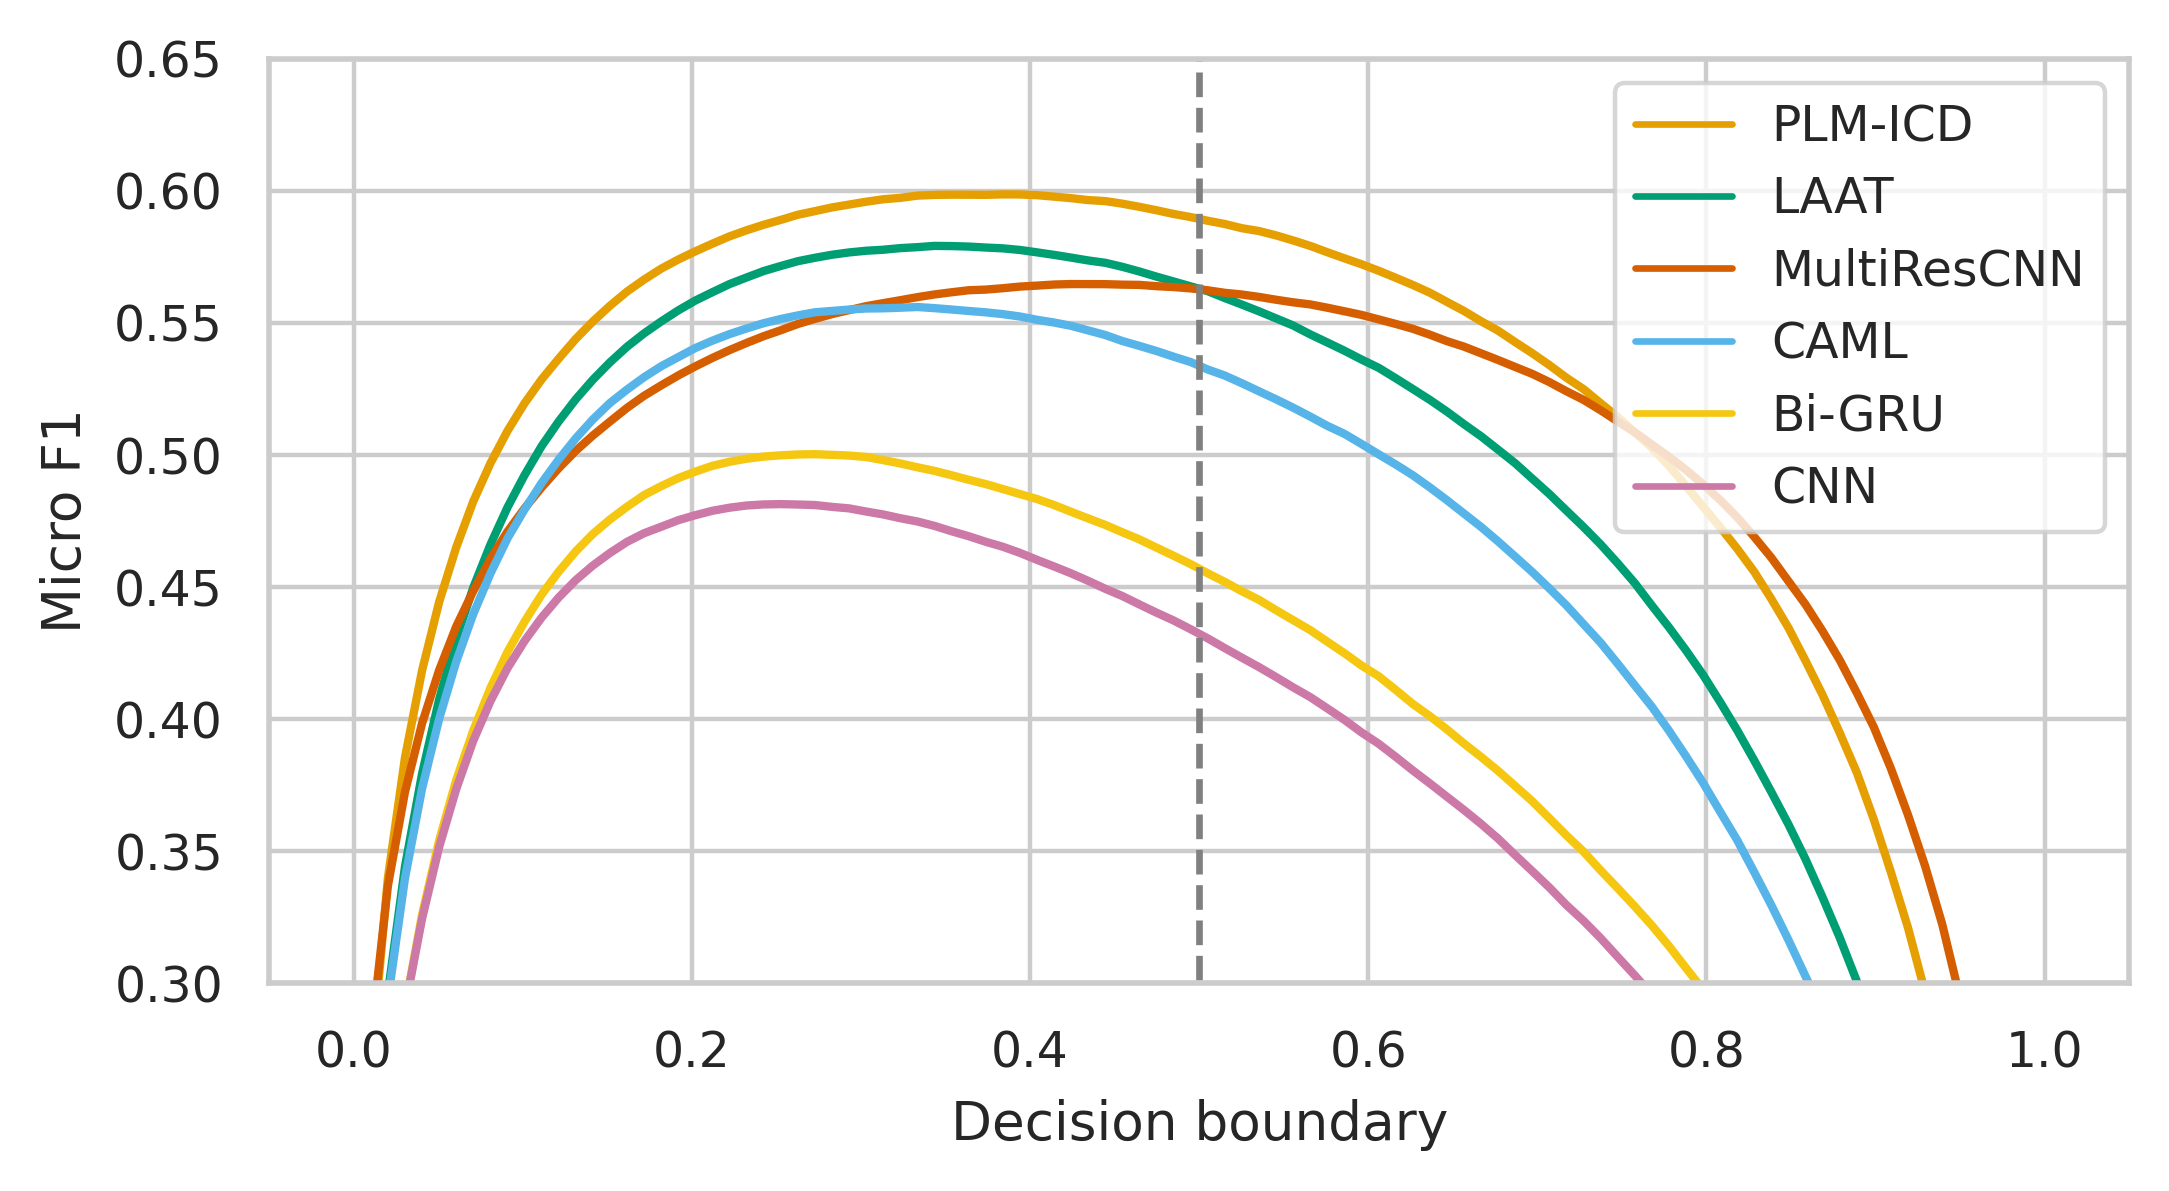
\includegraphics[width=\textwidth]{paper_automated/threshold_tuning_micro_full.png}
        % \caption{}
        % \label{fig:threshold_tuning_micro}
    \end{subfigure}
    \begin{subfigure}[b]{0.9\textwidth}
        \centering
        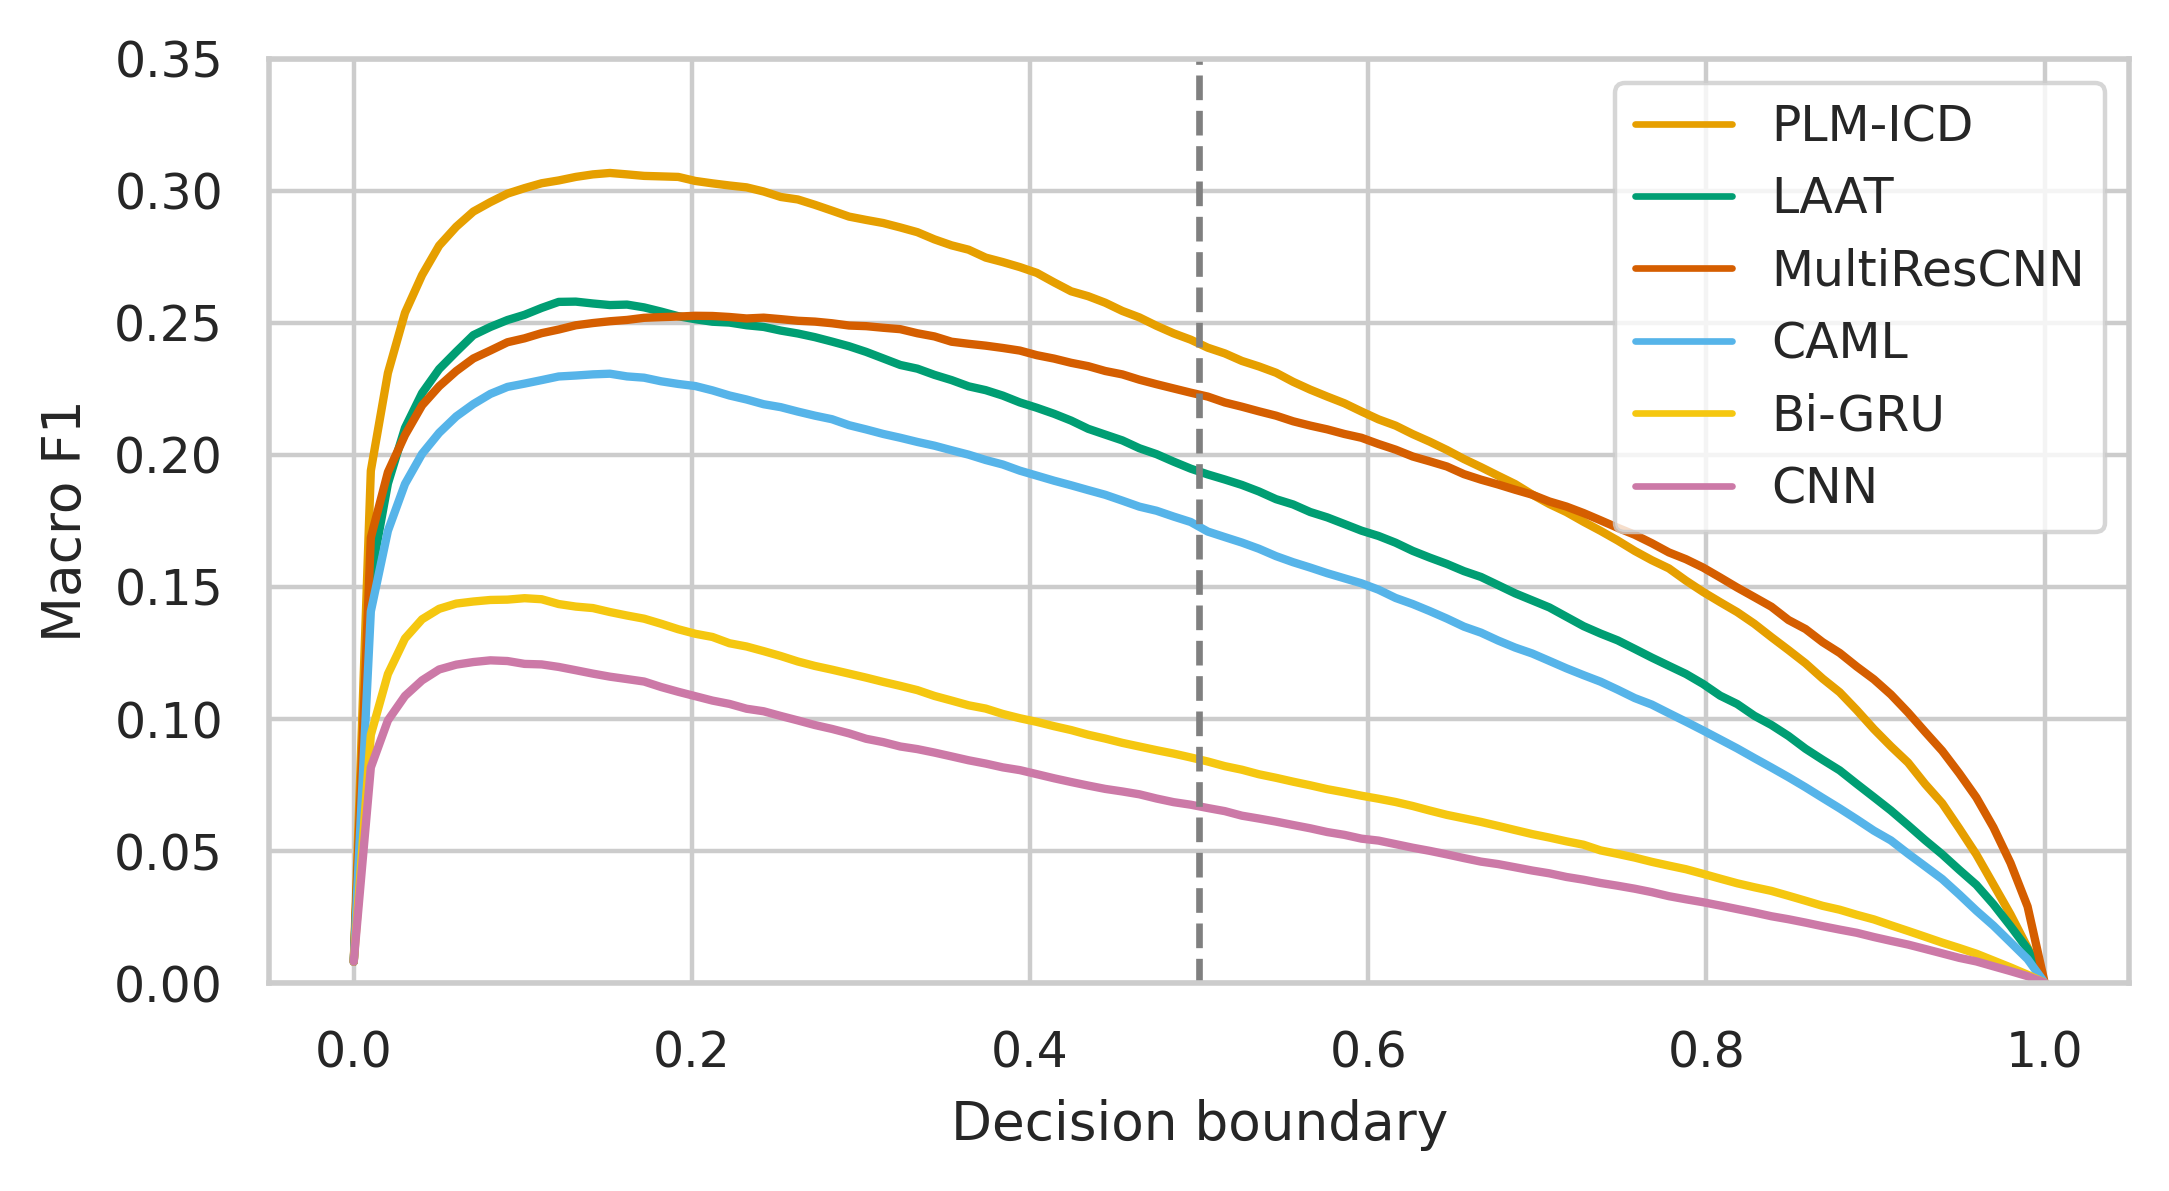
\includegraphics[width=\textwidth]{paper_automated/threshold_tuning_macro_full.png}
        % \caption{}
        % \label{fig:threshold_tuning_macro}
    \end{subfigure}%
    \caption[Relationship between chosen threshold and F1-score of every reproduced model.]{ The relationship between chosen threshold and F1-score of every reproduced model in \cref{tab:reproduced_results}. The left figure shows the micro F1-score, and the right shows the macro F1-score. The models were evaluated on MIMIC-III \textit{clean}.}
    \label{fig:threshold_tuning}
\end{figure}


\subsection{Error analysis}

\paragraph{Amount of training data:}

\cref{fig:train_size} shows the relationship between the number of training examples and the micro and macro F1-scores for all models.
In most cases, increasing the training data had a larger effect on the macro F1-score than the micro F1-score, indicating more extensive improvements in rare codes than common codes. The curve for macro F1 is less smooth because the decision boundary was tuned on the micro F1-scores.

\begin{figure}
    \centering
    \begin{subfigure}[b]{0.95\textwidth}
        \centering
        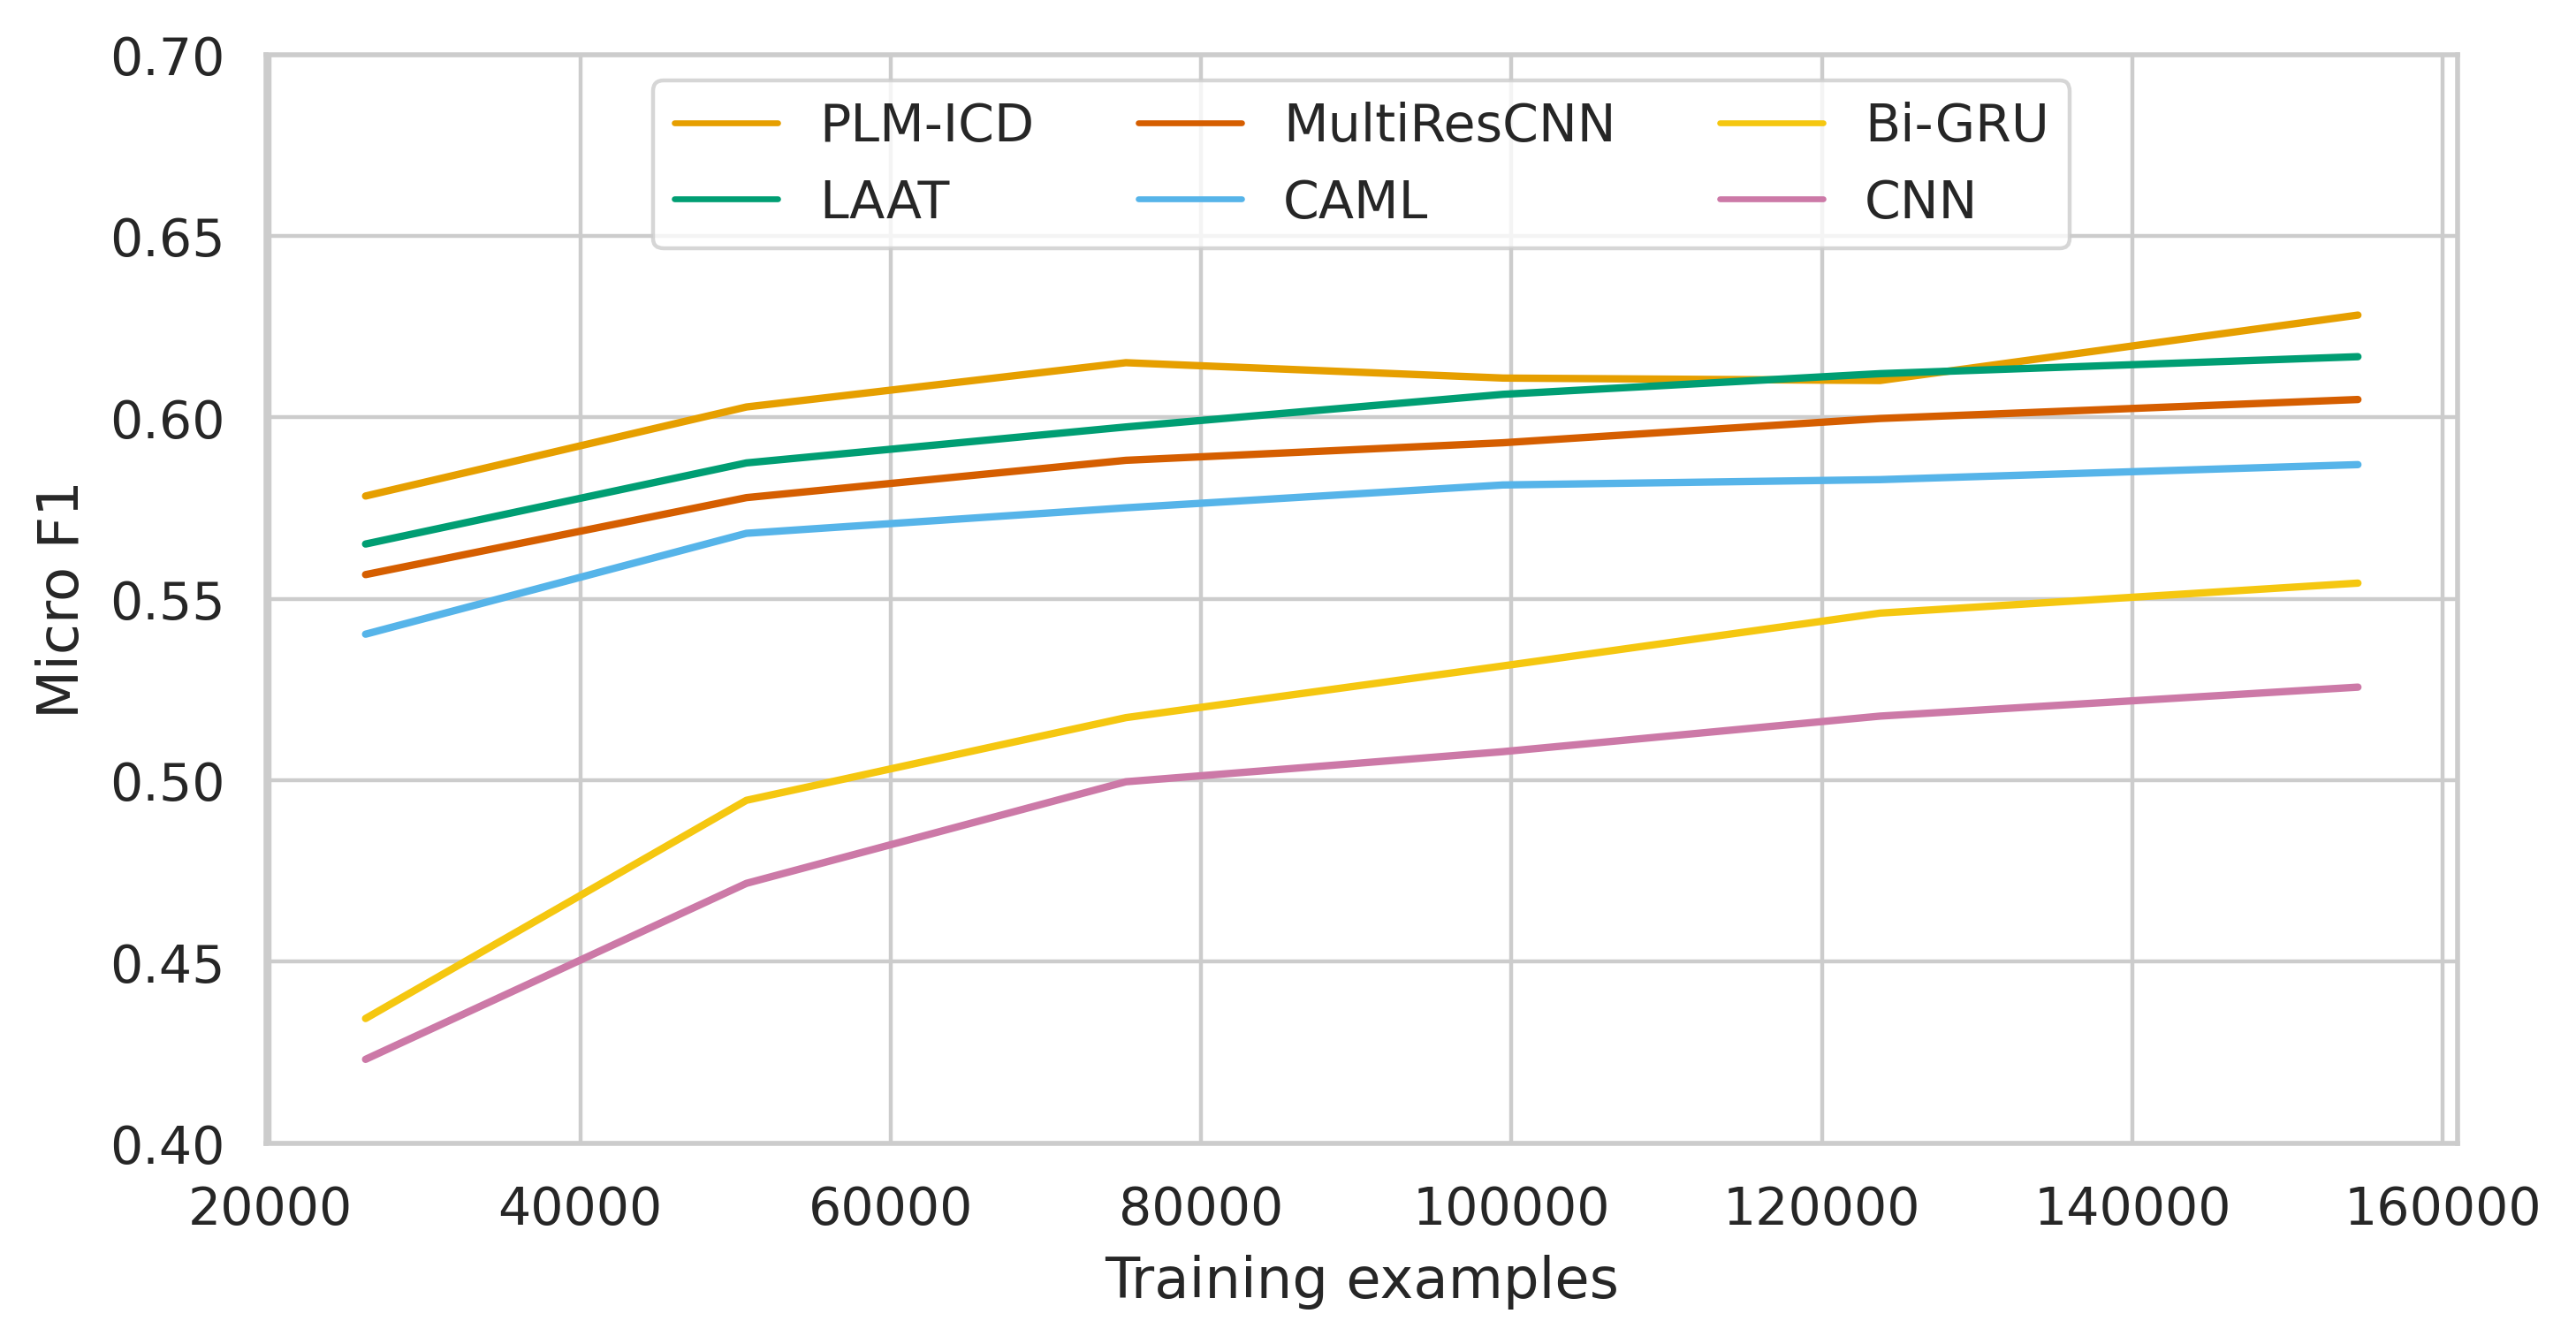
\includegraphics[width=\textwidth]{paper_automated/train_size_f1_micro.png}
        % \caption{}
        % \label{fig:train_size_micro}
    \end{subfigure}
    \begin{subfigure}[b]{0.95\textwidth}
        \centering
        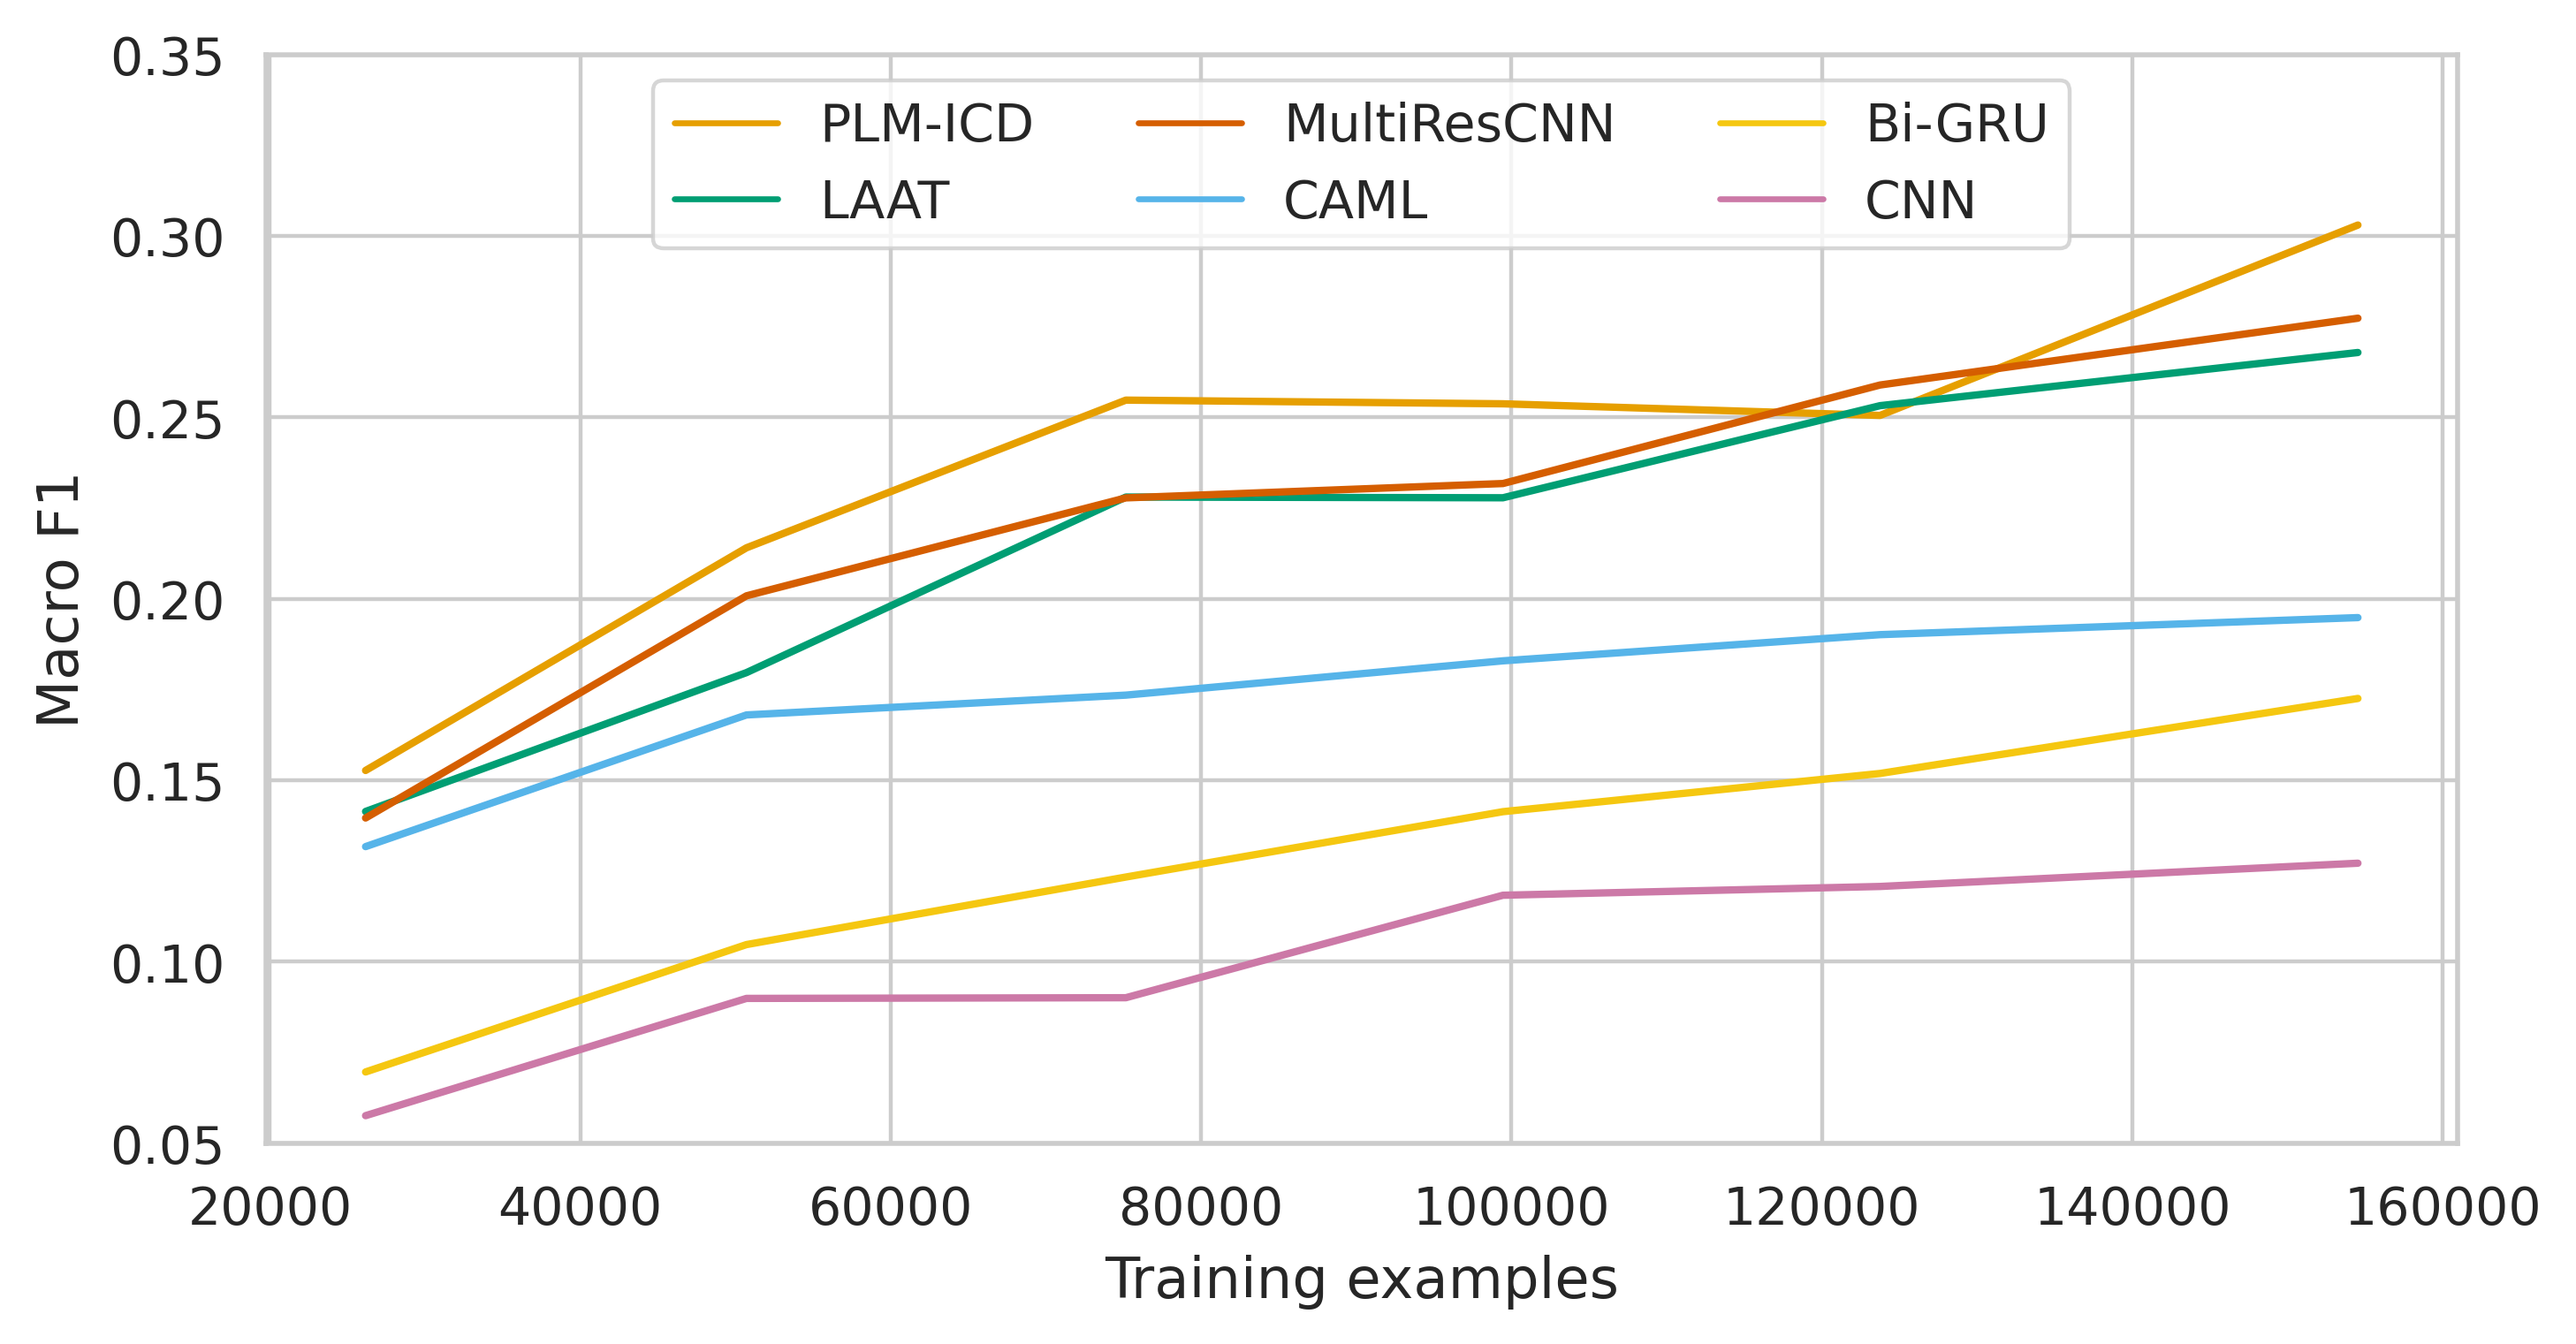
\includegraphics[width=\textwidth]{paper_automated/train_size_f1_macro.png}
        % \caption{}
        % \label{fig:train_size_macro}
    \end{subfigure}
    \caption[The relationship between the number of training examples and F1-score on MIMIC-IV \textit{ICD-9}.]{  The relationship between the number of training examples and F1-score on MIMIC-IV \textit{ICD-9}. The left figure shows the F1 Micro score on the y-axis, while the right figure shows the F1 Macro score.}
    \label{fig:train_size}
\end{figure}


\paragraph{Document length:}\label{subsubsec:document-length}

We plot the micro F1-score for all models as a function of the number of words per document in \cref{fig:text_length}. 
We note that all models underperformed on documents with fewer than 1000 words. 
By manual inspection, we found that most of these documents missed the information necessary to predict their labeled codes, leading to underperformance. 
In \cref{tab:correlations}, we list the Pearson and Spearman correlations. We excluded documents shorter than 1000 words to avoid confounding with missing information and longer than 4000 words due to the truncation limit. We observe a very small negative correlation between document length and micro F1 which matches the downward trend in micro F1, starting from approximately 1000 words in \cref{fig:text_length}. 
Although document length may itself be the cause of the slightly lower performance for long documents, there may be other factors correlated with document length impacting performance, such as the number of codes per document and code frequency.
As there are few long documents, the effect on average micro F1 for each dataset is negligible; hence, previous claims that long documents lead to poor performance in AMC could not be validated. Results on MIMIC-IV \textit{ICD-10} and MIMIC-III \textit{clean} were similar.

\begin{figure}
    \centering
    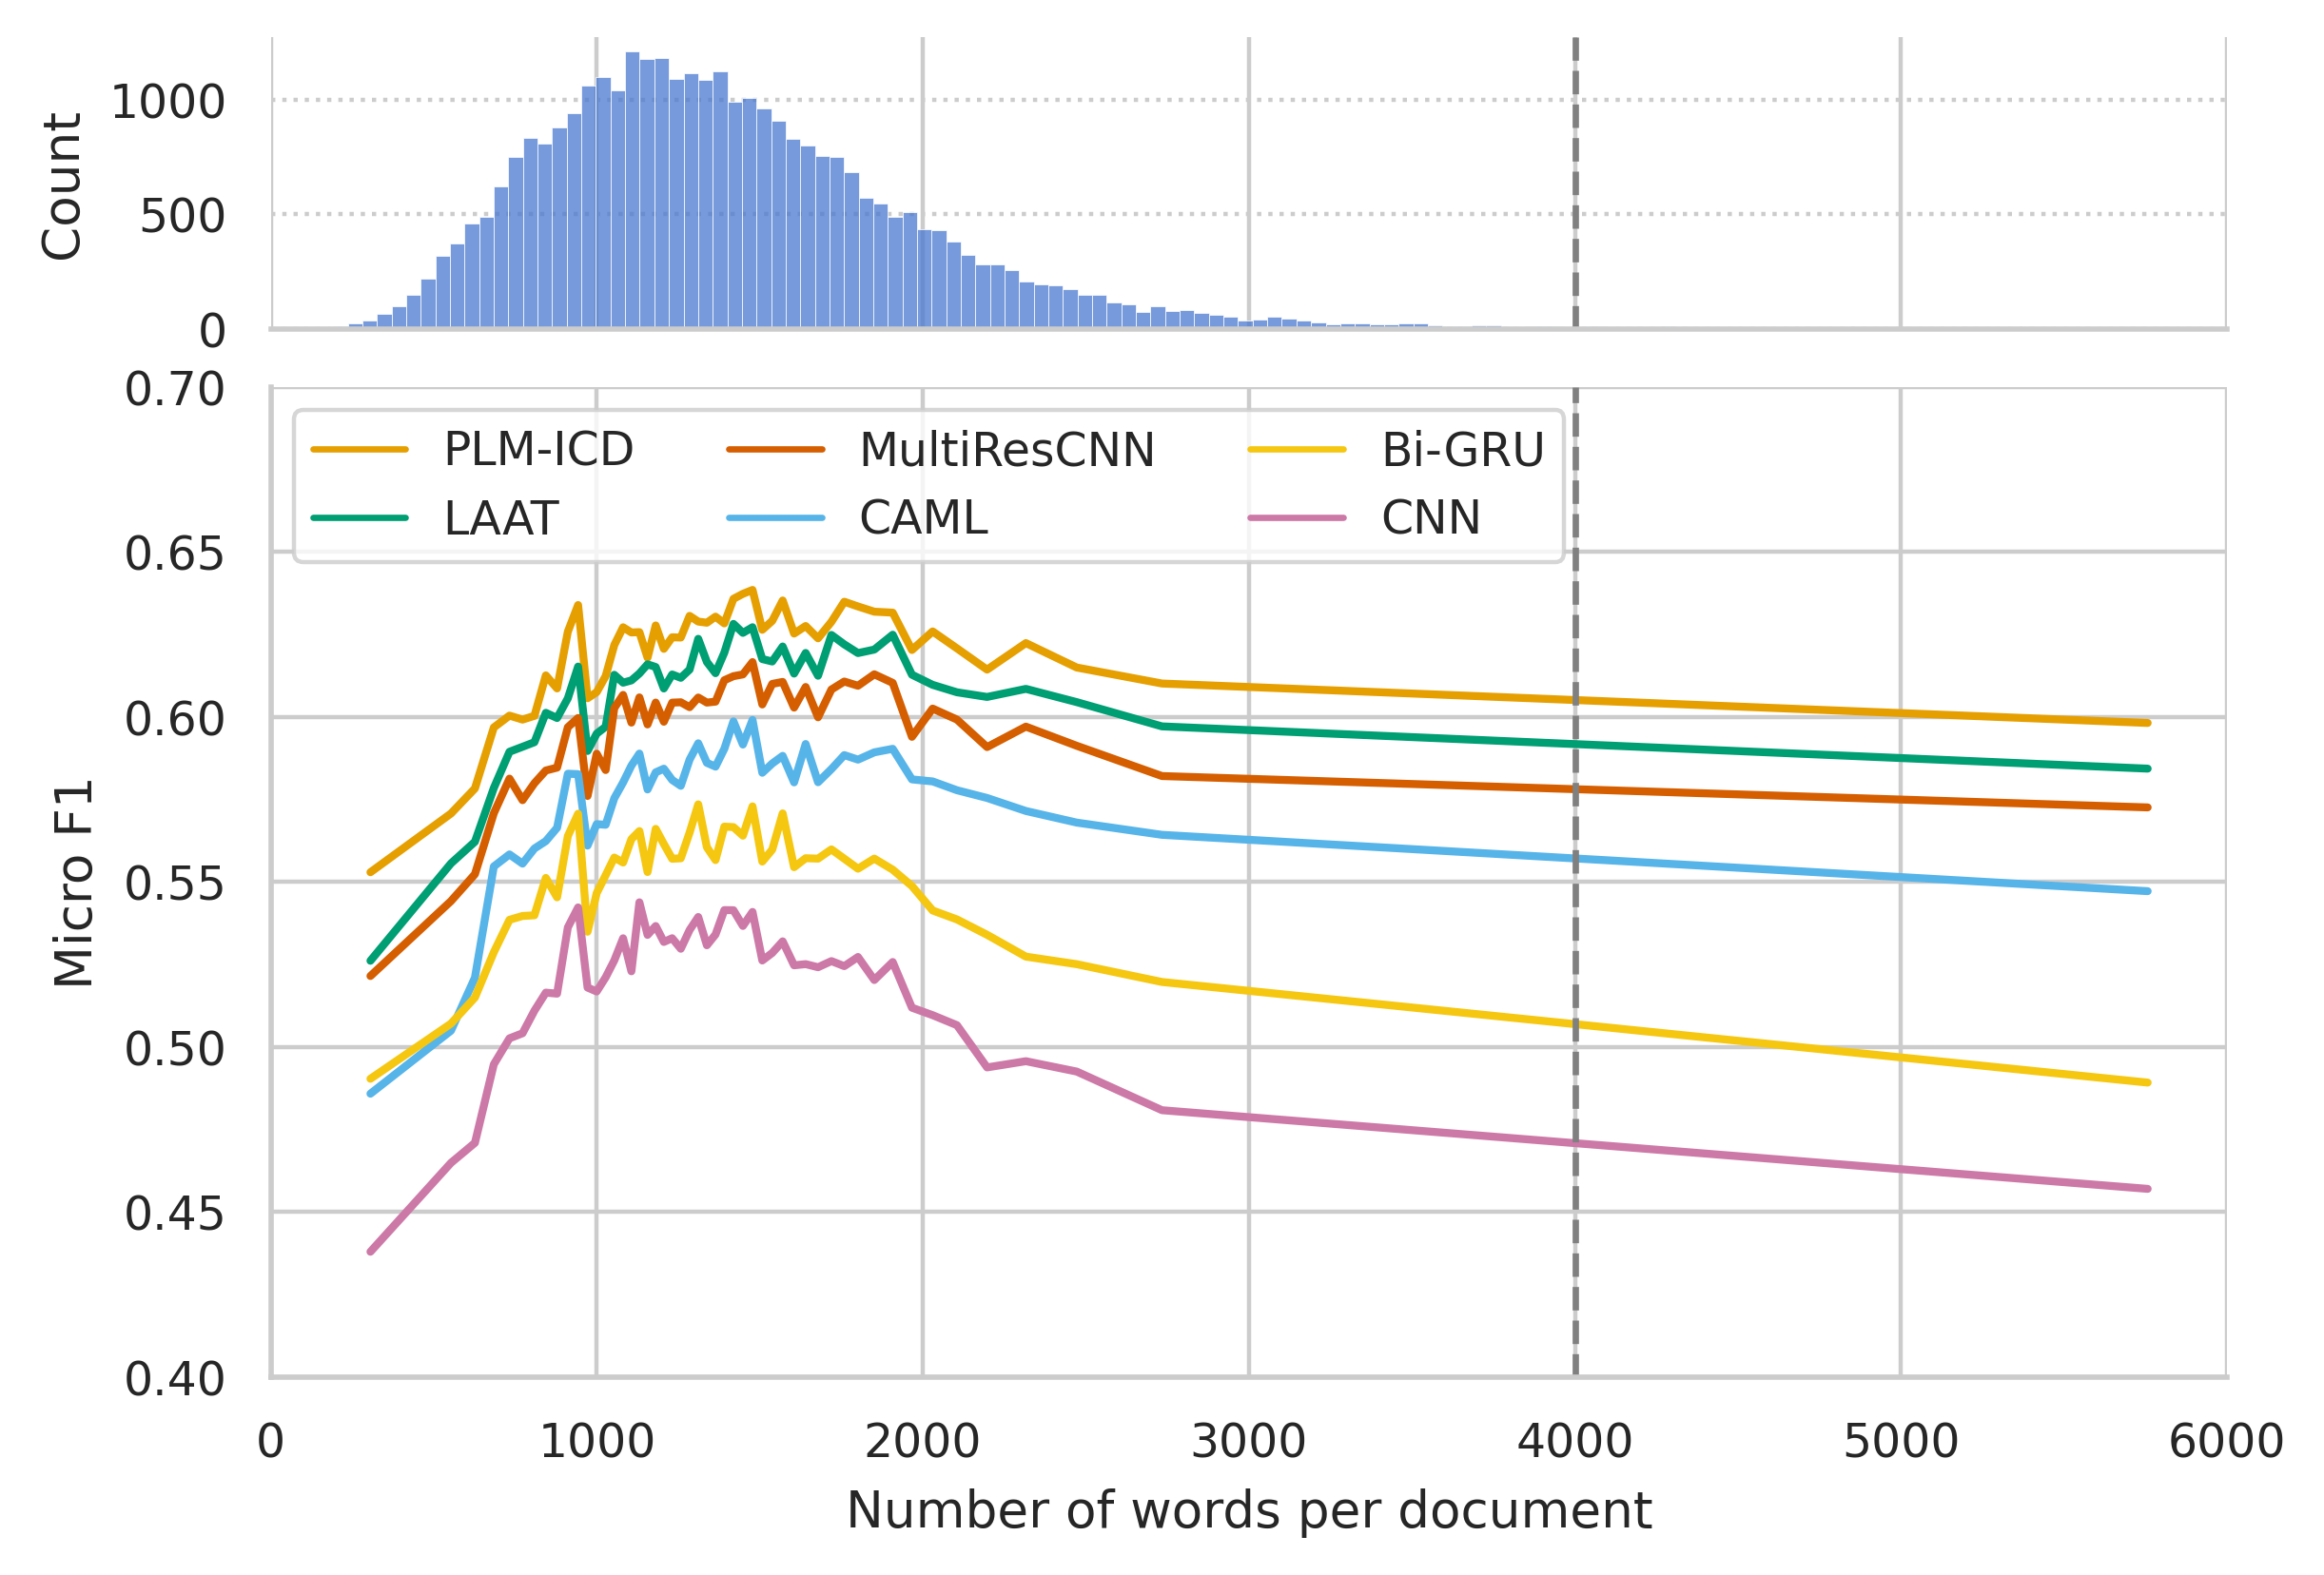
\includegraphics[width=0.9\textwidth]{paper_automated/f1_micro_vs_num_words.png}
    \caption[Relationship between the lengths of the clinical notes and the micro F1-score for each model on MIMIC-IV \textit{ICD-9}.]{Relationship between the lengths of the clinical notes and the micro F1-score for each model on MIMIC-IV \textit{ICD-9}. The vertical line indicates the maximum length of the notes after truncation. The histogram at the top visualizes the document length distribution.}
    \label{fig:text_length}
\end{figure}

\begin{table}
    \centering
    \caption[Correlation between the F1-score and the logarithm of code frequency and document length on MIMIC-IV \textit{ICD-9}.]{ Correlation between the F1-score and the logarithm of code frequency and document length on MIMIC-IV \textit{ICD-9}. As discussed in \cref{subsubsec:document-length}, we only considered document lengths between 1000 and 4000 words. All correlations are statistically significant ($p<0.001$).}
    \label{tab:correlations}
    \begin{tabular}{lcccc}
        \toprule
        & \multicolumn{2}{c}{Code frequency} & \multicolumn{2}{c}{Document lengths}\\
        \cmidrule(lr){2-3}\cmidrule(lr){4-5}
        & Pearson & Spearman & Pearson & Spearman \\
        \midrule
        CNN  & 0.61 & 0.68 & -0.09 & -0.08 \\
        Bi-GRU & 0.57 & 0.65 & -0.08 & -0.07 \\
        CAML & 0.56 & 0.60 & -0.03 & -0.03   \\
        MultiResCNN & 0.47 & 0.53 & -0.02 & -0.03  \\
        LAAT & 0.52 & 0.57 & -0.02 & -0.02 \\
        PLM-ICD & 0.48 & 0.52 & -0.02 & -0.02   \\
        \bottomrule
    \end{tabular}
\end{table}


\paragraph{Code analysis:}

\Cref{fig:icd9_vs_icd10} compares the best performing model, PLM-ICD, trained and evaluated on MIMIC-IV \textit{ICD-9} and \textit{ICD-10}. Similar results were obtained on MIMIC-III \textit{clean}.
The comparison shows the relationship between code frequencies in the training set and macro F1-scores. As shown in \cref{tab:fair_results}, all models perform worse on \textit{ICD-10} compared to \textit{ICD-9}. However, \cref{fig:icd9_vs_icd10} demonstrates that performance on codes with similar frequencies is comparable between the two splits. This suggests that the performance differences in \cref{tab:fair_results} are due to \textit{ICD-10} containing a higher fraction of rare codes as shown in \cref{fig:mimiciv_code_dist,fig:icd9_vs_icd10}.

The Pearson and Spearman correlations between the logarithm of code frequency and F1-score are shown in \cref{tab:correlations} for MIMIC-IV \textit{ICD-9}. Similar correlations were observed for the other datasets. All the models show moderately high correlation confirming that performance on rare codes is generally lower than on common codes. To further our understanding of the problem, we computed the percentage of unique codes in each dataset that the models never predicted. As seen in \cref{tab:missed_classes}, no model correctly predicted more than 50\% of the ICD-10 codes.

\Cref{fig:chapter_performance} shows the performance of PLM-ICD on each ICD-10 chapter---the top-most level in the tree-like hierarchy. 
For our analysis, we limited the scope to only focus on the diagnosis codes. We also excluded codes with fewer than one hundred training examples to control for some chapters having many rare codes. 

Overall, PLM-ICD never correctly predicted 2,928 of the 5,794 ICD-10 diagnosis codes in our split. Of these codes, only 110 had over a hundred training examples, and 58 belong to only two of the 20 chapters in MIMIC-IV \textit{ICD-10}. Specifically, 45 belong to the chapter relating to ``external causes of morbidity" (Z00-Z99), while 13 relate to ``factors influencing health status and contact with health services" (V00-Y99). To further investigate why most non-predicted codes with more than 100 training examples belong to only two chapters, we manually inspected a selection of codes in these chapters, as described in the following.

The Z68 category, part of the Z00-Z99 chapter, contains codes related to the patient's body mass index (BMI). Codes within this category occur more than 17,000 times in the MIMIC-IV training data, but PLM-ICD never predicts 20 out of the 26 codes of Z68. One possible hypothesis is that PLM-ICD struggles with extracting the BMI from the discharge summaries, as all digits have been removed in the pre-processing. We found several other codes containing digits in the code descriptions that the model failed to detect, e.g., ``Blood alcohol level of less than 20 mg/100 ml" (Y90.0), ``34 weeks gestation of pregnancy" (Z3A.34), and ``NIHSS score 15" (R29.715). These observations support our hypothesis that removing digits in the pre-processing makes certain codes challenging to predict.

The Y92 category, part of the V00-Y99 chapter, contains codes related to the physical location of occurrence of the external cause. It is a large category of 246 unique codes occurring 27,870 times in the training set. The category is challenging due to locations being very specific. For instance, there are unique codes for whether an incident occurred on a tennis court, squash court, art gallery, or museum. We hypothesize that the level of detail in the discharge summaries does not always match the fine-grained code differences.

\begin{figure}
    \centering
    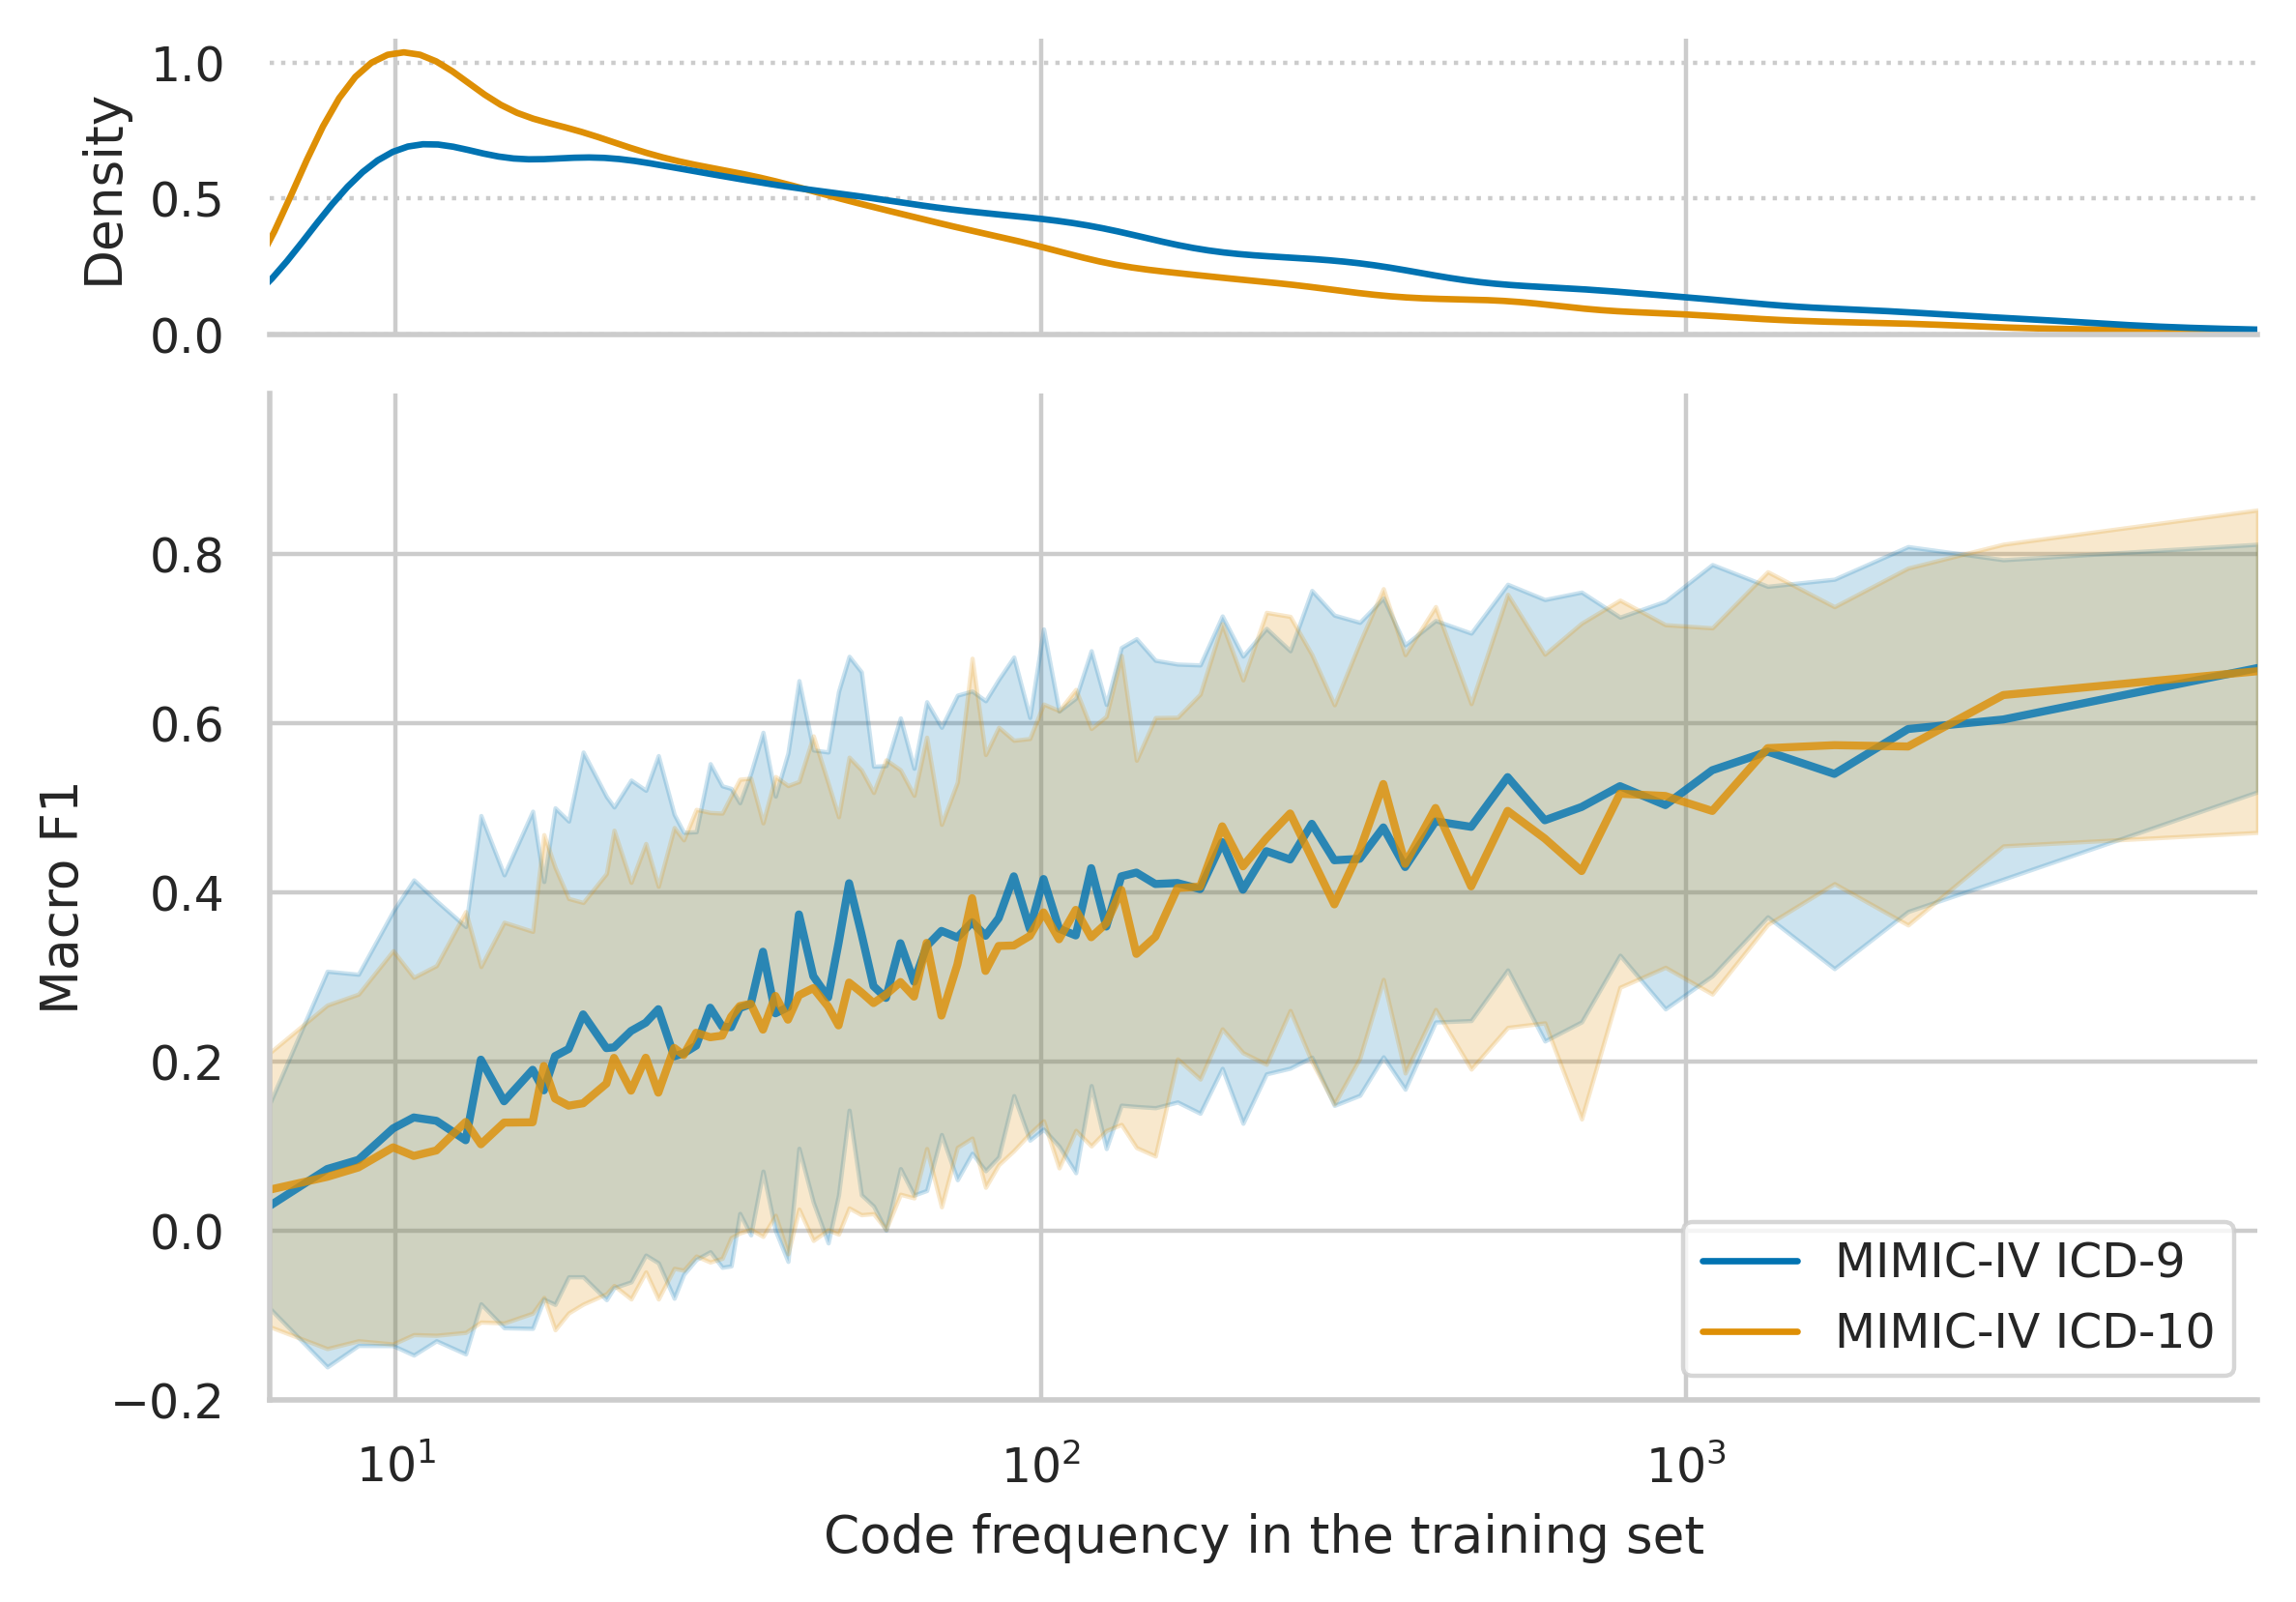
\includegraphics[width=0.9\textwidth]{paper_automated/code_count_vs_f1_all_datasets.png}
    \caption[Relationship between code frequencies and macro F1-score for PLM-ICD on MIMIC-IV \textit{ICD-9} and \textit{ICD-10}.]{Relationship between the code frequencies in the training set and the macro F1-score for PLM-ICD on MIMIC-IV \textit{ICD-9} and \textit{ICD-10}. The shaded area indicates the standard deviation of the score computed for codes within the bin.}
    \label{fig:icd9_vs_icd10}
\end{figure}

There are ten different codes in MIMIC-IV \textit{ICD-10} relating to nicotine dependence and tobacco use. The three most common are Z87.891 (``Personal history of nicotine dependence"), F17.210 (``Nicotine dependence, cigarettes, uncomplicated"), and Z72.0 (``Tobacco use"), with 26,427, 8,486, and 1,914 training examples, respectively. Among these, Z72.0 was the third most common single code in the training set that PLM-ICD never predicted correctly. PLM-ICD achieved an F1-score of 53\% for Z87.891, 51\% for F17.210, and 0\% for Z72.0 and all other nicotine-related codes. These findings suggest that when there is a class imbalance among highly similar codes, PLM-ICD is strongly biased toward the most frequent ones.

 \begin{table}
    \centering
    \caption{Percentage of ICD diagnosis codes in the test set that the models never predicted correctly.}
    \label{tab:missed_classes}
    \begin{tabular}{lccc}
        \toprule
        & MIMIC-III & \multicolumn{2}{c}{MIMIC-IV}\\
        \cmidrule(lr){2-2}\cmidrule(lr){3-4}
        & \textit{clean} &  \textit{ICD-9} & \textit{ICD-10} \\
        \midrule
        CNN  & 68.2 & 61.5 & 72.0\\
        Bi-GRU  & 65.0 & 54.3 & 67.1\\
        CAML & 52.8 & 57.0 & 62.0  \\
        MultiResCNN  & 48.8 & 40.3 & 53.5 \\
        LAAT  & 50.4 & 43.6 & 55.0\\
        PLM-ICD   & 44.3 & 39.3 & 51.8\\
        \bottomrule
    \end{tabular}
\end{table}


\begin{figure}
    \centering
    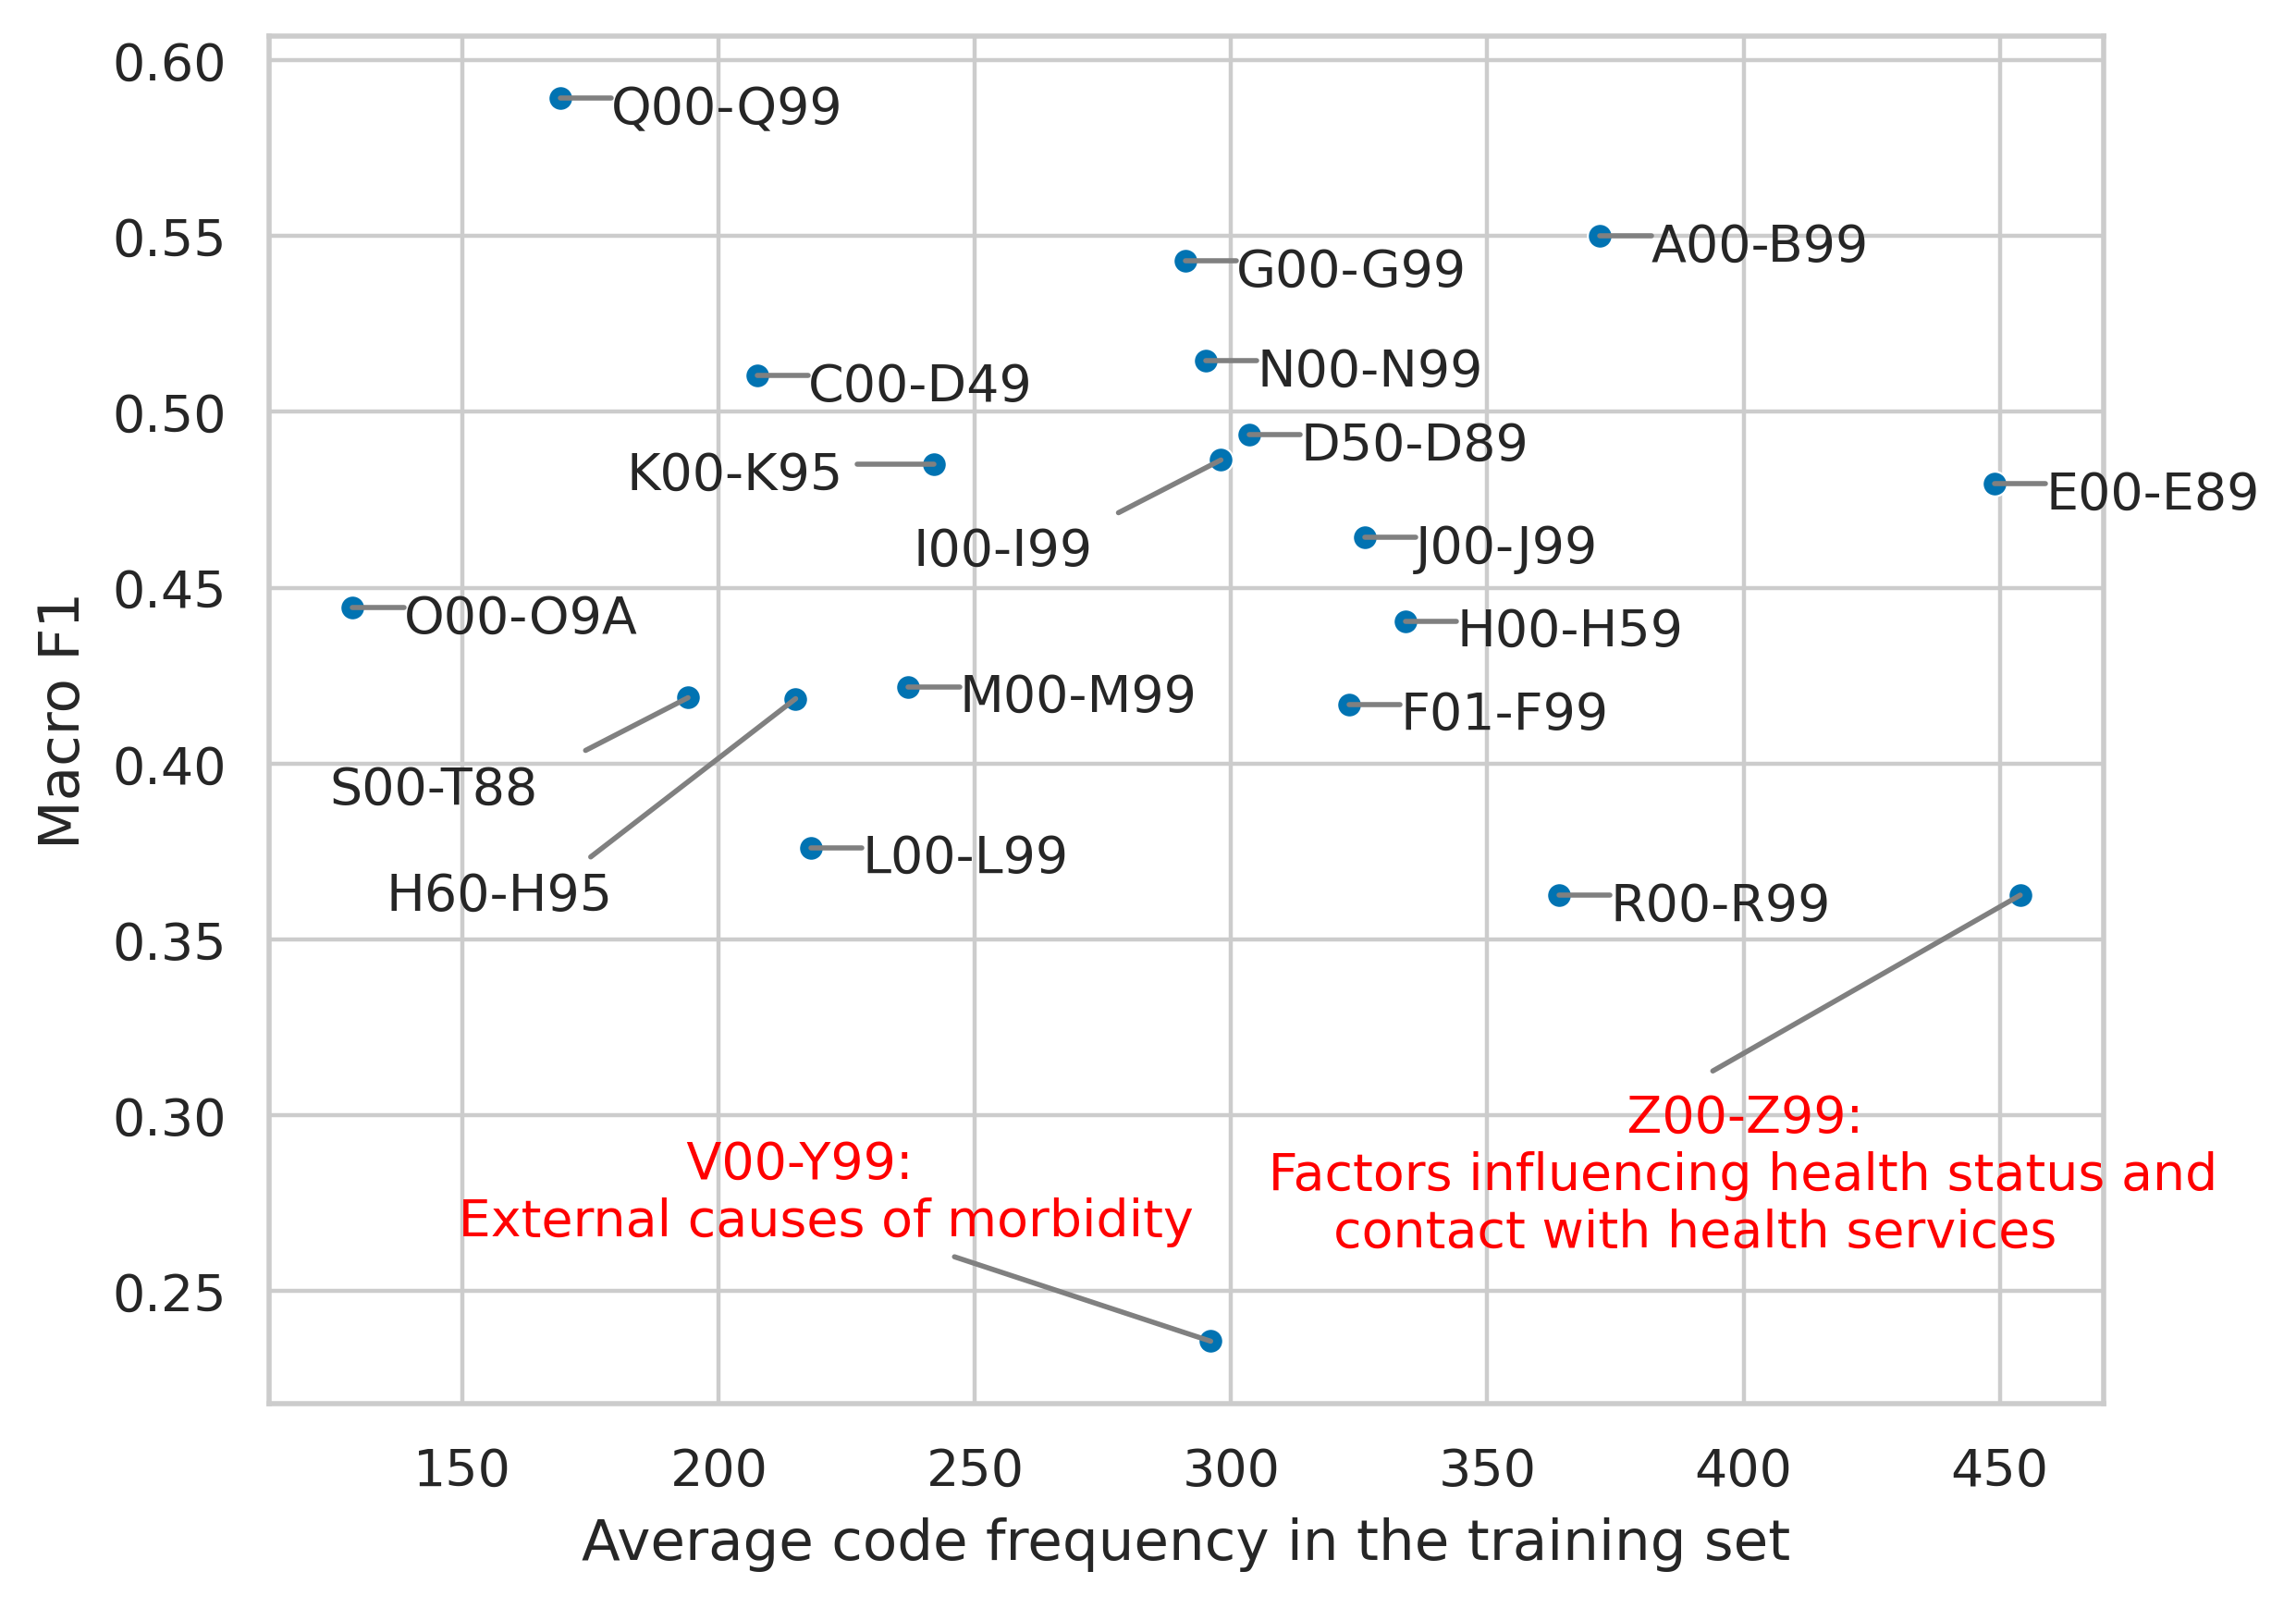
\includegraphics[width=0.9\textwidth]{paper_automated/chapters.png}
    \caption[Performance of PLM-ICD on ICD-10 chapters.]{Performance of PLM-ICD on ICD-10 chapters. Only codes with more than a hundred occurrences in the MIIMC-IV ICD-10 training set were considered, leaving 20 chapters. We found Z00-Z99 and V00-Y99 to be the most challenging.}
    \label{fig:chapter_performance}
\end{figure}




\section{Discussion}
\subsection{Lessons learned}
We found reproducing the results of CNN, Bi-GRU, CAML, and LAAT challenging. While we expected discrepancies due to random weight initializations and data shuffling, the differences from the original works exceeded our presuppositions. Our reproduced results were better than originally reported for Bi-GRU and CNN and worse for CAML and LAAT on most metrics. There have been multiple reports of issues in reproducing the results of \textcite{mullenbachExplainablePredictionMedical2018}.\footnote{\url{https://github.com/jamesmullenbach/caml-mimic}} Additionally, most previous works did not report which version of MIMIC-III they used, and the code and hyperparameter configurations were not documented in detail. Therefore, we hypothesize that our results differ because previous works report incorrect hyperparameters or use an earlier version of MIMIC-III.

We showed that models previously reported as low-performing underperformed partly due to a poor selection of hyperparameters and not tuning the decision boundary. In our revised comparison, we demonstrated that training the models using our setup decreased the difference between the best and worst micro F1-scores by $5.8$ percentage points. \textcite{mullenbachExplainablePredictionMedical2018} concluded that CNN outperformed Bi-GRU. However, in our revised comparison, Bi-GRU outperformed CNN on all metrics on MIMIC-III \textit{clean}, MIMIC-IV \textit{ICD-9}, and MIMIC-IV \textit{ICD-10}.

Even though MultiResCNN contains more parameters than CAML, \textcite{liICDCodingClinical2020} concluded that MultiResCNN was faster to train because it converged in fewer epochs. However, this was only true when using the original setup where CAML converged after 84 epochs. We found that when using a learning rate schedule and appropriate hyperparameters, it was possible to train all the models in 20 epochs without sacrificing performance. Therefore, with our setup, CAML was faster to train than MultiResCNN.

We demonstrated that the macro F1-score had been underestimated in prior works due to the poorly sampled MIMIC-III \textit{full} split and the practice of setting the F1-score of all codes absent in the test set to 0. Since 54\% of the codes in MIMIC-III \textit{full} are missing in the test set, the maximum possible macro F1-score is 46\%. The previously highest reported macro F1-score on MIMIC-III \textit{full} is 12.7\% for PLM-ICD~\parencite{kimReadAttendCode2021}. Using our corrected macro F1-score on the same split, PLM-ICD achieved a macro F1-score of 22.8\%. This large difference from previous state-of-the-art seems to indicate that all previous work on AMC used the suboptimally calculated macro F1-score, including works not reproduced in this paper. Many studies use the macro F1-score to evaluate the ability of their models to predict rare codes \parencite{kimReadAttendCode2021, yuanCodeSynonymsMatter2022}. If it has indeed been incorrectly calculated in these studies, some conclusions drawn in previous work regarding rare code prediction may have been misguided.

Multiple studies mention lack of training data, rare codes, and long documents as the main challenges of AMC \parencite{dongExplainableAutomatedCoding2021,feuchtDescriptionbasedLabelAttention2021,huangPLMICDAutomaticICD2022,jiDoesMagicBERT2021,liICDCodingClinical2020,liuEffectiveConvolutionalAttention2021,moonsComparisonDeepLearning2020,pascualBERTbasedAutomaticICD2021,tengReviewDeepNeural2022,tengExplainablePredictionMedical2020, vuLabelAttentionModel2020, venkateshAutomatingOverburdenedClinical2023}. In the error analysis, we aimed to validate or falsify these assumptions. We found that rare codes were challenging for all models and observed that more than half of all ICD-10 codes were never predicted correctly. Furthermore, in \cref{fig:train_size}, we showed that when adding more training data, most models see a greater performance improvement on rare codes than on common codes. 
These findings suggest that medical coding is fundamentally challenged by a lack of training data that, in turn, gives rise to many rare codes.
We found that document length and model performance only exhibited a weak correlation. Specifically, the low number of very long documents was insufficient to affect the average performance on the dataset. 

\subsection{Future work}
We recommend future work within AMC use our revised comparison method, including stratified sampled splits of MIMIC datasets, corrected evaluation metrics, hyperparameter search, and decision boundary tuning to avoid reporting suboptimal or biased results. 
Furthermore, for AMC to become a viable solution for ICD-10, future research should focus on improving performance on rare codes while, in the shorter term, developing methods to detect codes that are too challenging for automated coding and, therefore, should be coded manually. Finally, while PLM-ICD outperforms the other models in this paper, the improvements are limited compared to the effect of pre"=training in other domains \parencite{mohamed_selfsupervised_2022, linPretrainedTransformersText2021,baevski_wav2vec_2020,devlin_bert_2018,dosovitskiy_image_2021}.
Notably, there have been several unsuccessful attempts at using pre"=trained transformers for medical coding \parencite{jiDoesMagicBERT2021,gaoLimitationsTransformersClinical2021,michalopoulosICDBigBirdContextualEmbedding2022,pascualBERTbasedAutomaticICD2021,zhangBERTXMLLargeScale2020}. In future work, we want to investigate why pre"=trained transformers underperform in medical coding.


\subsection{Limitations}
We presented findings and analyses on MIMIC-III and MIMIC-IV. It is unclear how our findings generalize to medical coding in real-world settings.
For instance, since MIMIC-III and IV contain data from the emergency department and ICU of a single hospital, the findings in this paper may not generalize to other departments or hospitals. 
For instance, discharge summaries from outpatient care are often easier to code than summaries from inpatient care as they are shorter with fewer codes per document \parencite{zhangBERTXMLLargeScale2020, liuEffectiveConvolutionalAttention2021, tsengAdministrativeCostsAssociated2018}.

The medical code labeling of MIMIC is used as a gold standard in this paper. However, medical coding is error-prone, and, in many cases, deciding between certain codes can be a subjective matter \parencite{nouraeiAuditNatureImpact2013, lloydPhysicianCodingErrors1985}. \textcite{burnsSystematicReviewDischarge2012} systematically reviewed studies assessing the accuracy of human medical coders and found an overall median accuracy of 83.2\% (IQR: 67.3–92.1\%). \textcite{searleExperimentalEvaluationDevelopment2020} investigated the quality of the human annotations in MIMIC-III and concluded that 35\% of the common codes were under-coded. Such errors and subjectivity in manual medical coding make model training and evaluation challenging and suggests that additional evaluation methods using, e.g., a human-in-the-loop, could be useful to increase the reliability of results. 

\section{Conclusion}
In this paper, we first reproduced the results of selected state-of-the-art models focusing on unimodal models with publically available source code. 
We found that model evaluation in original works was biased by an inappropriate formulation of the macro F1-score and treatment of missing classes in the test set. By fixing the macro F1 computation, we approximately doubled the macro F1 of the reproduced models on MIMIC-III \textit{full}. 
We introduced a new \textit{clean} split for MIMIC-III that contains all classes in the test set and performed a revised comparison of all models under the same training, evaluation, and experimental setup, including hyperparameter and decision boundary tuning. We observed a significant performance improvement for all models, with those previously reported as low-performing improving the most. 
We reported the first results of current state-of-the-art models on the newly released MIMIC-IV dataset \parencite{johnsonMIMICIVFreelyAccessible2023, goldbergerPhysioBankPhysioToolkitPhysioNet2000} and provided splits for the \textit{ICD-9} and \textit{ICD-10} coded subsets using the same method as for MIMIC-III \textit{clean}.
Through error analysis, we provided empirical evidence for multiple model weaknesses. Specifically, models underperform severely on rare codes 
and, in contrast to previous claims, long documents only have a negligible negative performance impact. 
We release our source code, model parameters, and the new MIMIC-III \textit{clean} and MIMIC-IV \textit{ICD-9} and \textit{ICD-10} splits.$^(\ref{footnote:source_code})$

\section*{Acknowledgments}
This research was partially funded by the Innovation Fund Denmark via the Industrial Ph.D. Program (grant no. 2050-00040B, 0153-00167B, 2051-00015B) and Academy of Finland (grant no. 322653).
We thank Sotiris Lamprinidis for implementing our stratification algorithm and data preprocessing helper functions.
   
}


\part[discussion and conclusions]{discussion and conclusions}\label{part:discussion-and-conclusion}
%!TEX root = ../thesis.tex

\chapter[discussion]{Discussion}\label{chp:discussion}
% ~5 pages
%
% OUTLINE:
% - paper-hierarchical:
%   - Suitability of VAEs for representation learning (minimization of mutual information and sensitivity to implicit prior such as architecture)
% - paper-benchmarking
%   - Inferiority of probabilistic methods compared to self"=supervised learning. 
% - 

The rapid progress of machine learning that started about a decade ago with the 2012 ImageNet competition and the work of \textcite{krizhevsky_imagenet_2012} all but slowed down during the course of this project. 
Following the papers by \textcite{choi_waic_2019,nalisnick_detecting_2019,hendrycks_deep_2019}, the field of out-of-distribution detection saw a surge of interest that has since grown yearly, while self"=supervised learning for speech has continued to advance with works such as CPC \parencite{oord_representation_2018}, wav2vec 2.0 \parencite{baevski_wav2vec_2020} and data2vec \parencite{baevski_data2vec_2022}. 

Having focused on VAEs for out-of-distribution detection in \cref{part:unsupervised-uncertainty-estimation} and on self"=supervised methods for representation learning in \cref{part:self-supervised-speech-representation-learning}, this discussion will bridge a gap between the two approaches and consider how VAEs might be enabled to learn representations more competitive with self"=supervised methods. 
Furthermore, since the work in \cref{part:medical-applications} only had limited focus on uncertainty, we will also present and discuss the use of calibration techniques for the stroke recognition model drawing connections to how such systems are perceived and used in practice. 


\section{Representation learning with variational autoencoders}
%
In this thesis we studied two different approaches to speech representation learning: VAEs in \cref{chp:paper-hierarchical,chp:paper-modelagnostic,chp:paper-benchmarking} and self"=supervised methods in \cref{chp:paper-review}. 
As we saw, the probabilistic formulation of VAEs provides benefits for their application to uncertainty quantification, although competitive methods that use self"=supervised foundation models have also been proposed \textcite{xiao_we_2021,hendrycks_using_2019,bergman_classificationbased_2020}. Self"=supervised methods are generally superior when it comes to performance on downstream tasks. While this of course depends on the task and the amount and type of unlabeled and labeled data, self"=supervised methods for speech are commonly evaluated on downstream tasks that are harder and more complex than those used for VAEs. For instance, between \cref{tab: phoneme recognition (PER),tab:unsupervisedASR} self"=supervised methods can be seen to outperform VAEs for phoneme recognition while self"=supervised methods are also reported for word-level speech recognition. 
In the following, we will discuss potential directions of future research that might help shed light on why VAEs representations underperform on downstream tasks and how they might be improved.


\paragraph{Designing the latent space} 
Architectural improvements and hierarchies of latent variables are two related, and interesting, approaches to learning more semantic features in VAEs. 
Some success has been demonstrated in the image domain with models like BIVA \parencite{maaloe_biva_2019}, NVAE \parencite{vahdat_nvae_2020}, and VD-VAE \parencite{child_very_2021}, with up to 78 stochastic layers, achieving tight likelihoods and high-quality samples, although limited effort has put towards using such models for downstream tasks. 
For speech, a hierarchical model operating on multiple temporal scales, such as the Clockwork VAE \parencite{saxena_clockwork_2021} adapted for speech in \cref{chp:paper-benchmarking}, might help better capture dependencies at longer ranges and encode more semantic features. 
For instance, phonetic content for pronunciation might be learned at lower layers, speaker identity at the upper layers, and semantic features, such as word-meaning, in between. 
Although some work has successfully separated speaker identity from content by modifying the latent variables and their dependencies \parencite{hsu_unsupervised_2017}, models that can learn a deep hierarchy of features for speech remains an open challenge. The work presented in \cref{chp:paper-benchmarking} represents an effort to make progress towards such a model. 


\paragraph{Adding a few labels} 
Another way to improve the representations learned in VAEs is via semi-supervised learning. 
Here, a few labels are used to inform which patterns that are learned from a large, mostly unlabeled, data set. 
This is usually done by defining a new stochastic variable as the target and deriving a semi-supervised version of the ELBO that accommodates using the labels when they are available, or marginalizing the target variable when they are not. The VAE is then trained on the labeled and unlabeled data simultaneously. 

Although VAEs are strong models for semi-supervised learning \parencite{kingma_semi-supervised_2014,kingma_improved_2016,maaloe_biva_2019}, self"=supervised methods have established themselves as superior for most tasks in this setting \cite{baevski_wav2vec_2020,jiang_speech_2021, liu_learning_2023}. 
Despite being theoretically appealing, joint objectives for semi-supervised learning in VAEs have practical drawbacks. By training on labeled and unlabeled data simultaneously, semi-supervised VAEs are often less flexible than are self"=supervised methods that divide the training into two separate phases. By first fitting a general foundation model in an expensive pre"=training phase it can then later be fine"=tuned for many downstream tasks, at relatively low cost. 
VAEs, on the other hand, must often learn the labeled downstream tasks while simultaneously training on the unlabeled data. This is computationally expensive, but also requires retraining with the unlabeled data, when new supervised data becomes available or a new task is added. 


\paragraph*{Approximating less}
VAE are inherently approximate. Training is performed on a lower bound of the likelihood and inference is variational, amortized and for non-hierarchical models, mean field. As a consequence, the gradient itself is estimated inexactly, usually by only one posterior sample, leading to non-negligible variance. 
For that reason, it seems plausible that using tighter bounds and reducing gradient variance improve representation learning in VAEs. 
Importance weighting the ELBO \parencite{burda_importance_2016} provides a tight bound on the likelihood, reduces gradient variance, and induces a complex implicit posterior distribution. 
Its use has become standard when reporting likelihood benchmarks but as we described in \cref{sec:variational-autoencoders}, \textcite{rainforth_tighter_2019} demonstrated that using it during training introduces high gradient variance for the inference network hurting its ability to learn useful representations. Later works largely solved this issue \parencite{roeder_sticking_2017,tucker_doubly_2019,bauer_generalized_2021} and showed that the reduced variance leads to improved likelihoods. 

Despite much of this progress being prior to the latest, very large hierarchical VAEs, such as BIVA \parencite{maaloe_biva_2019}, NVAE \parencite{vahdat_nvae_2020}, and VD-VAE \parencite{child_very_2021}, these models are all trained with the single-sample ELBO using regularly reparameterized gradient estimator. Instead, these models rely on advanced inference networks \parencite{maaloe_biva_2019} and architectural improvements \parencite{vahdat_nvae_2020, child_very_2021} to overcome the challenges of training hierarchical VAEs. 
This seems to indicate that there might be untapped potential in consolidating the work on low-variance gradient estimators and advanced architectures and inference networks.


\paragraph{Masking} 
As discussed in \cref{chp:paper-review}, masking is one of the driving techniques behind the success of self"=supervised methods for speech \parencite{devlin_bert_2018,baevski_wav2vec_2020}. By removing tokens from the input or an early feature extraction layer and tasking a model with inferring their representations, models are forced to learn how neighboring tokens relate to those masked. Depending on the size of the mask, these dependencies can be more or less semantic in nature. For instance, the wav2vec 2.0 model is well-known to learn representations that have high similarity with word identity and meaning \parencite{pasad_layerwise_2021}. 

In comparison, reconstruction in VAEs is done from latent variables that are inferred from the full, unmasked input. Since all information is generally available, this might allow the encoder and decoder models to perform well for reconstruction, even with no, or limited, use of contextual dependencies. Furthermore, VAE reconstruction almost always targets the direct input in order to learn the distribution over the training data and to enable generating new samples. However, compared to many self"=supervised methods that target intermediate, learned representations, this forces VAEs to encode all aspects of the input that are important to its distribution. As we saw in \cref{chp:paper-hierarchical}, this will generally include low-level features that are necessary for accurate input reconstruction. Such features require large latent space representations and model capacity \parencite{vahdat_nvae_2020,child_very_2021}, but are usually of lesser interest for downstream tasks \parencite{baevski_wav2vec_2020}.

Since the ELBO does not immediately allow for masking as part of the training, it has been only sparsely examined for VAEs. Specifically, masking has seen the most attention for VAEs within missing data imputation. In this setting, the input is partially observed, and often represented as a segmentation into observed and missing parts via a mask that indicates where the data is missing. The model is then trained to infer the latent variable from the observed data and reconstruction also deals only with the observed data. 
By comparison to self"=supervised approaches that use masking for representation learning, the missing data setting of VAEs focuses on reconstructing the observed data rather than the missing, which might not lead to the same benefits in representation learning. 

The idea of using VAEs to impute missing data was already examined in the seminal paper by \textcite{rezende_stochastic_2014}. Here the model was trained with fully observed data and used to impute data in an iterative sampling approach post hoc, leaving the learned representations unchanged.
Previous work that trains on partially observed data has largely focused on the ability of these models to yield high-quality imputations within the tabular and image data domains and have not probed for the effects on the learned latent representation \parencite{mattei_miwae_2019, ipsen_not-miwae_2021}. 

Including masked objectives into the principled probabilistic framework of VAEs might require creative thinking, but it seems likely that relaxing the requirement of exact input reconstruction and enforcing the need of encoding (and decoding) contextual information could lead the way for future types of VAEs to learn representations that are competitive with self"=supervised methods.


\paragraph{Giving up?}



\parencite{tomczak_trouble_2022}
\parencite{huszar_is_2017}

\lesstodo[inline]{Discuss whether VAEs are even suitable for representation learning due to them minimizing a mutual information term in the ELBO (derive this form).}
\lesstodo[inline]{Discuss sensitivity to ``implicit" prior such as architecture (and probably optimization method and other). Include reference to \parencite{huszar_is_2017} discussing the usefulness of using a maximum likelihood objective for representation learning in generative models.}




\lesstodo[inline]{Out-of-distribution detection on speech?}






% \subsection{Uncertainty estimation with self-supervised methods}
% %

% \textcite{pasad_layerwise_2021} found that layers 6-7 hold the most information about phonetic content and word identity and meaning for \texttt{wav2vec2-base}. 
% For \texttt{wav2vec2-large} the phonetic content is highest in layers 11 and 18-19 with a drop in between, while word identity and meaning are highest between layers 12 and 18. 


% Uncertainty of representations versus uncertainty of downstream task outputs. 
% % \textcite{wickstrom_relax_2023} propose a method for quantifying uncertainty based on 




% \section{\Cref{chp:paper-review} revisited: \dots} \label{sec:discussion-paper-review}

% \lesstodo[inline]{Are self"=supervised speech representations useful for unsupervised uncertainty estimation? \parencite{nava_stateconsistency_2021, nava_uncertaintyaware_2021} Within robotics but not really related.}
% % Since the main focus within self"=supervised learning has been on improving downstream task performance, very limited work, if any, has investigated self"=supervised representations in terms of uncertainty estimation. 
% % However, in the context of medical applications where data can be abundant but labels are sparse, unsupervised uncertainty estimation is a very interesting direction for future work.
% \lesstodo[inline]{OOD data: Generalization or detection (https://arxiv.org/pdf/2110.11334.pdf)?}




\section{\Cref{chp:paper-retrospective} revisited: Calibration}

\begin{figure}
    \centering
    \begin{subfigure}[c]{0.49\columnwidth}
        \centering
        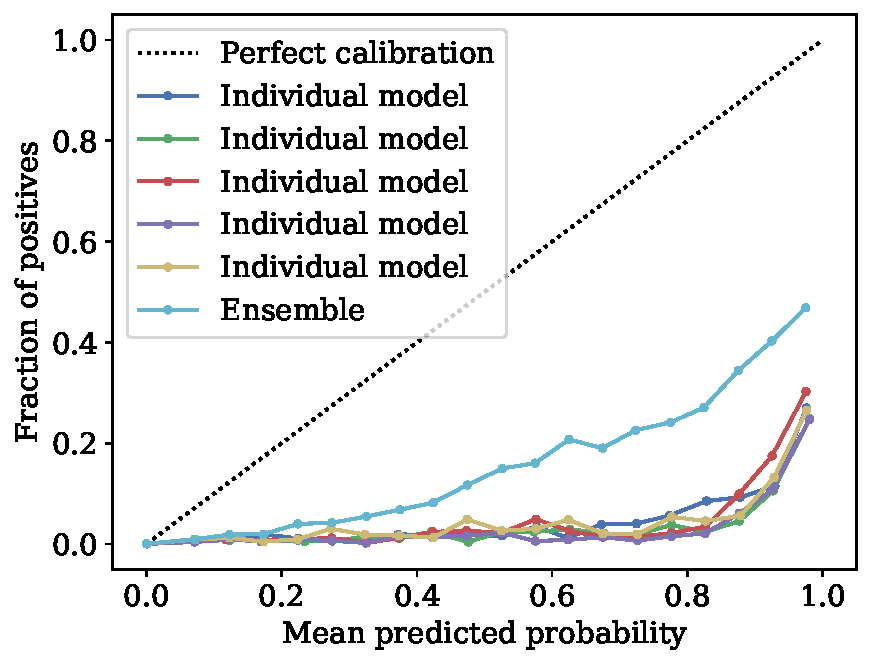
\includegraphics[width=1\columnwidth]{paper_retrospective_calibration_plots/calibration_curve_ensemble_and_all_models_uncalibrated.pdf}
        % \caption{}
        % \label{fig_discussion:calibration_curve_ensemble_and_all_models_uncalibrated}
    \end{subfigure}
    \hfill
    \begin{subfigure}[c]{0.49\columnwidth}
        \centering
        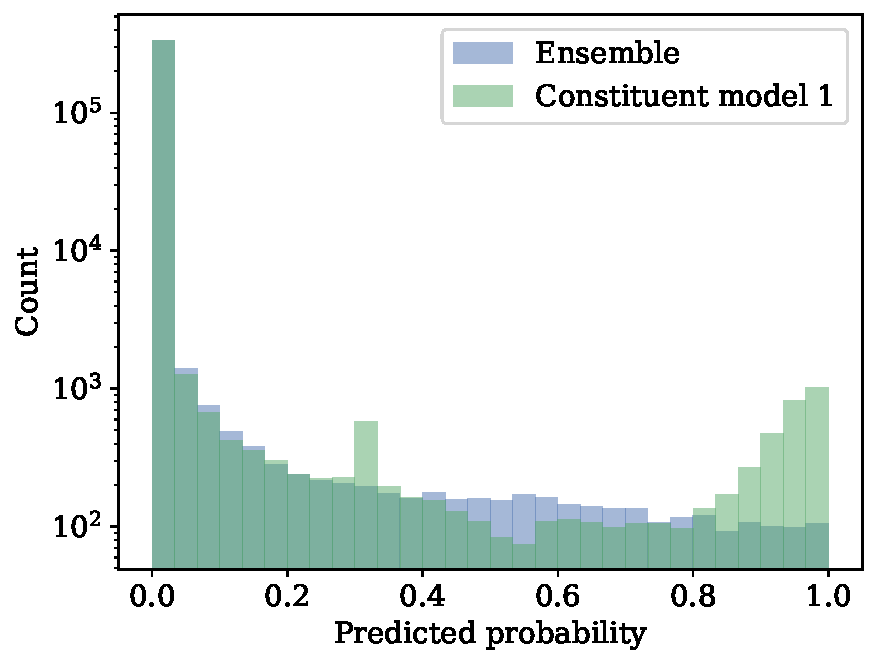
\includegraphics[width=1\columnwidth]{paper_retrospective_calibration_plots/histogram_ensemble_and_single_model.pdf}
        % \caption{}
        % \label{fig_discussion:histogram_ensemble_and_single_model}
    \end{subfigure}
    \caption[Calibration curve for the uncalibrated stroke recognition ensemble and empirical distribution of predicted probabilities.]{ Calibration curve for the uncalibrated stroke recognition ensemble (left) and the histogram of predicted probabilities (right) for the test set. We use the ensemble that achieved the median F1-score reported in \cref{fig_retrospective:figure1-roc-curve} and \cref{tab_retrospective:table3-occlusion-analysis}.}
    \label{fig_discussion:retrospective-paper-calibration-curve-of-uncalibrated-model}
\end{figure}

Our work on stroke recognition in \cref{chp:paper-retrospective} focuses on the predictive performance of the ensemble model and an analysis of feature importance, but does not explicitly consider uncertainty estimation. 
As we discussed in \cref{subsec:model-calibration}, such a model can be calibrated to predict probabilities that are aligned with the empirical probability of the model being correct on some validation set. Here we present and discuss model calibration for the ensemble model. 

We compute the calibration curve by sorting the probabilities predicted on the test set into a number of bins spanning the range from zero to one. For each bin $b$, we compute the mean predicted probability $\bar{p}$ and the fraction of examples for which the model predicted correctly $r_{b}$. The calibration curve is the drawn from the $\{(\bar{p}_{b}, r_{b})\}_b$ pairs. For any given bin, a perfectly calibrated model would have the same fraction of correct predictions as that bin's mean value, $\bar{p}_{b} = r_{b}\,\forall\,b$. 

The calibration curve for the uncalibrated stroke recognition ensemble and its constituent models is plotted in \cref{fig_discussion:retrospective-paper-calibration-curve-of-uncalibrated-model} along with a histogram of its predicted probabilities. The miscalibration issue that we previously discussed is clearly visible as a strong overconfidence for both ensemble and constituents, although the ensemble is much better calibrated than its constituents. Since the ensemble's output probability is computed as the harmonic mean of the five constituent model probabilities, it can never exceed the maximum probability predicted between the constituent models. This property tends to make ensemble probabilities less extreme and, since the constituent models are overconfident, this results in better calibration (see also the histogram in \cref{fig_discussion:retrospective-paper-calibration-curve-of-uncalibrated-model}). 

\begin{figure}
    \centering
    \begin{subfigure}[c]{0.49\columnwidth}
        \centering
        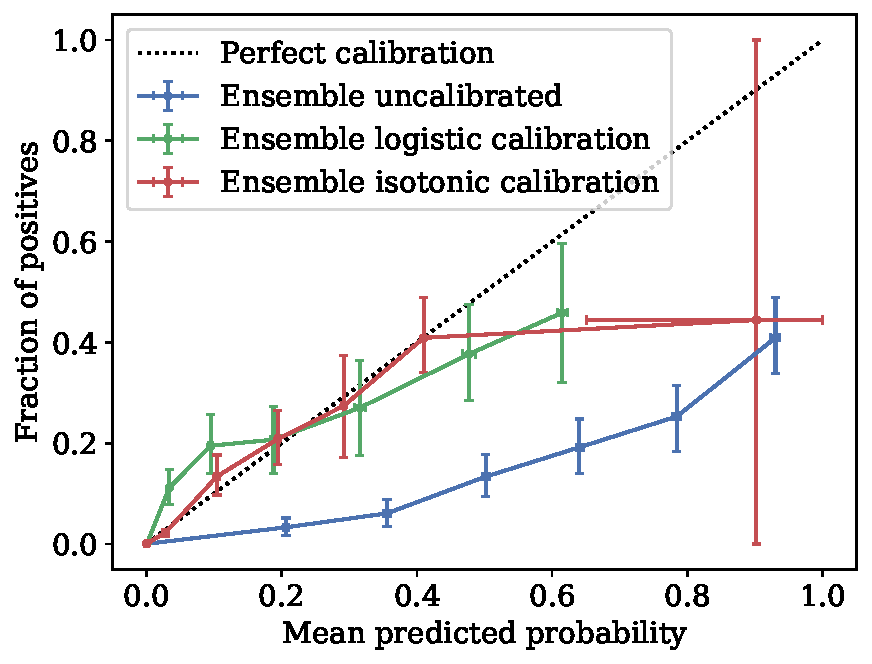
\includegraphics[width=1\columnwidth]{paper_retrospective_calibration_plots/calibration_curves_ensemble_with_cis.pdf}
    \end{subfigure}
    \hfill
    \begin{subfigure}[c]{0.49\columnwidth}
        \centering
        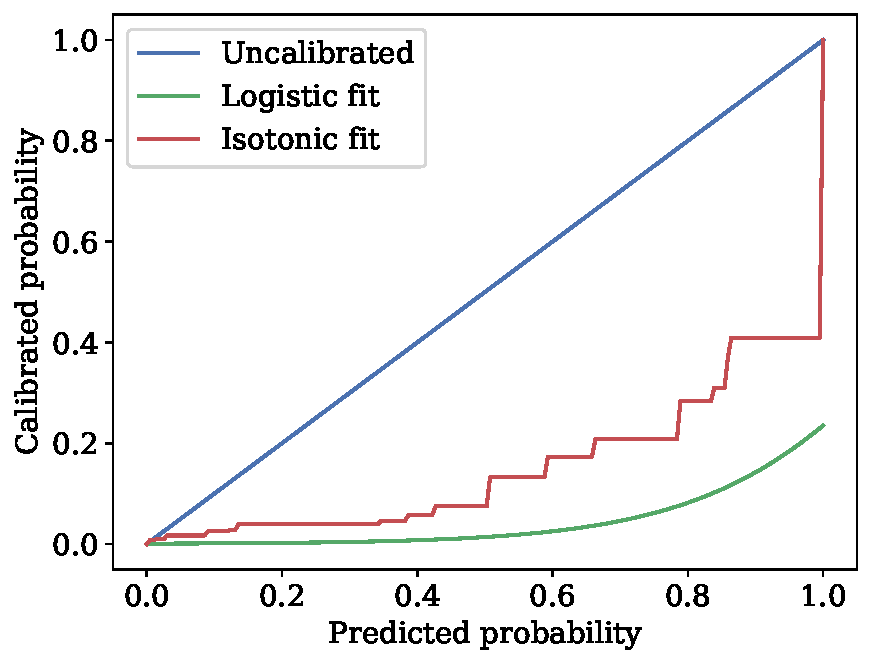
\includegraphics[width=1\columnwidth]{paper_retrospective_calibration_plots/calibration_fits_ensemble.pdf}
    \end{subfigure}    
    \caption[Calibration fits and curves for the stroke recognition ensemble using Platt-scaling and isotonic regression for calibration.]{ Calibration curves using sigmoid and isotonic calibration fits for the stroke recognition ensemble model (left) and the calibration fits (right) for the test set. We use the ensemble that achieved the median F1-score reported in \cref{fig_retrospective:figure1-roc-curve} and \cref{tab_retrospective:table3-occlusion-analysis}.}
    \label{fig_discussion:retrospective-paper-calibration-curve-sigmoid-isotonic}
\end{figure}

To calibrate the ensemble model, we can use methods such as Platt-scaling \parencite{platt_probabilistic_1999} or isotonic regression \parencite{zadrozny_transforming_2002}. 
In either case, we fit a simple regression model (logistic or isotonic) to the predicted probabilities and the target labels on the validation set and use it to adjust the probabilities predicted on the test set. We show the resulting calibration curves on the left in \cref{fig_discussion:retrospective-paper-calibration-curve-sigmoid-isotonic} and the logistic and isotonic fits on the right with 95\% bootstrap confidence intervals on the bin centers ($x$ error) and fraction of positives ($y$ error). 
% In \cref{fig_discussion:retrospective-paper-calibration-curve-sigmoid-isotonic} we have done so for the ensemble model and visualize the results on the test set. 
% On the left, we plot the resulting calibration curves and on the right we show the logistic and isotonic fits. 
We see that both methods result in quite good calibrations\footnote{Brier scores on test set: Uncalibrated = $0.003500$, logistic = $0.001807$, isotonic = $0.001774$. Relative improvement in Brier score compared to uncalibrated (Brier skill score): Logistic = $0.4830$, isotonic = $0.4924$.} and that the predicted probabilities are shifted towards smaller values. 
Since stroke cases have low prevalence, high probability is predicted only for a few examples (see histogram in \cref{fig_discussion:retrospective-paper-calibration-curve-of-uncalibrated-model}). This leads to a lack of data for the calibration fits at high predicted probabilities which can be seen to result in poor generalization to the test set, especially for the nonparametric isotonic regression.

% Brier scores:  {'uncalibrated': 0.0034955788687128925, 'logistic': 0.0018072483306197486, 'isotonic': 0.0017744177396100578, 'average': 0.0021955477869598783}
% BSS uncalibrated reference:  {'logistic': 0.48299025755205005, 'isotonic': 0.4923822902432705}
% BSS mean reference:  {'logistic': 0.17685766561145932, 'isotonic': 0.1918109229282361}

\begin{figure}
    \centering
    \begin{subfigure}[c]{0.49\columnwidth}
        \centering
        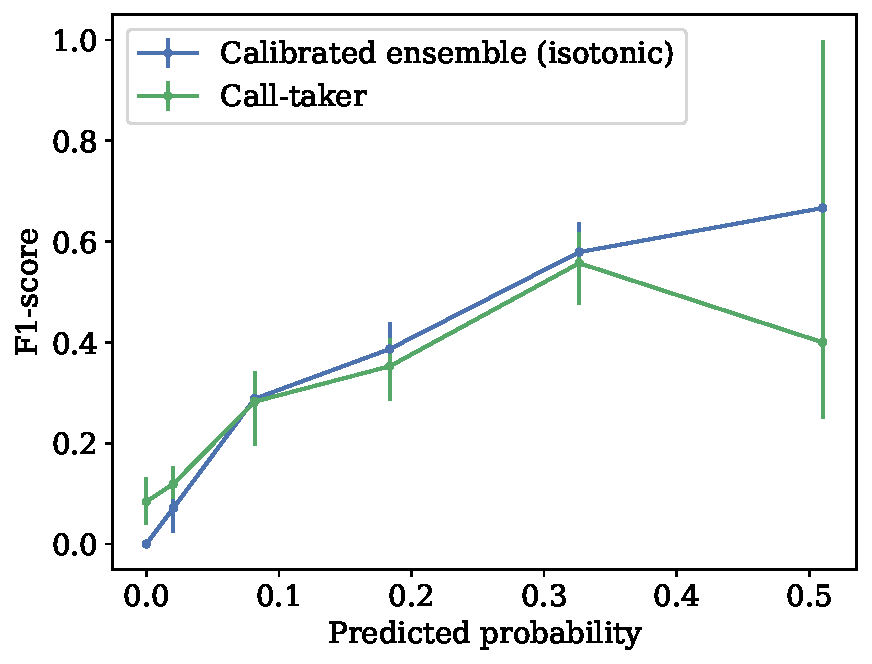
\includegraphics[width=1\columnwidth]{paper_retrospective_calibration_plots/f1_score_vs_predicted_probability_ensemble_calltaker_with_cis.pdf}
    \end{subfigure}
    \hfill
    \begin{subfigure}[c]{0.49\columnwidth}
        \centering
        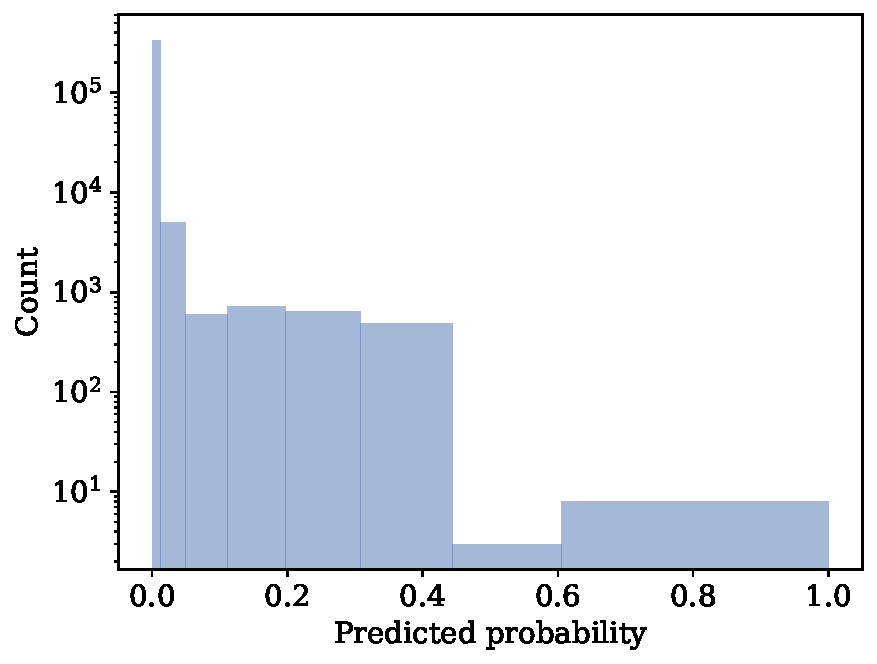
\includegraphics[width=1\columnwidth]{paper_retrospective_calibration_plots/predicted_probability_histogram.pdf}
    \end{subfigure}    
    \caption[Comparison of F1-score of stroke recognition ensemble and call-takers as function of predicted probability.]{ Comparison of the F1-score of the stroke recognition ensemble and call-takers. The F1-score is computed on subsets of the test dataset made by binning on the predicted probabilities of the calibrated ensemble. We see that the relative performance improvement of the ensemble over call-takers is higher towards more certain predictions. We use the ensemble that achieved the median F1-score reported in \cref{fig_retrospective:figure1-roc-curve} and \cref{tab_retrospective:table3-occlusion-analysis}.}
    \label{fig_discussion:retrospective-paper-f1-performance-vs-predicted-probability}
    % \begin{subfigure}[c]{0.49\columnwidth}
    %     \centering
    %     \includegraphics[width=1\columnwidth]{paper_retrospective_calibration_plots/precision_vs_predicted_probability_ensemble_calltaker_with_cis.pdf}
    %     % \caption{}
    %     % \label{fig_discussion:calibration_curve_ensemble_and_all_models_uncalibrated}
    % \end{subfigure}    
    % % \hfill
    % \begin{subfigure}[c]{0.49\columnwidth}
    %     \centering
    %     \includegraphics[width=1\columnwidth]{paper_retrospective_calibration_plots/recall_vs_predicted_probability_ensemble_calltaker_with_cis.pdf}
    %     % \caption{}
    %     % \label{fig_discussion:histogram_ensemble_and_single_model}
    % \end{subfigure}
\end{figure}

Clinicians in intensive care units and emergency departments have been found to strongly agree that a singular focus on overall accuracy cannot alone ensure sustained trust in a model \cite{tonekaboni_what_2019}. Clinicians expect an alert to present a prediction that aligns with patient status. Despite expert-agreed thresholds for when alerts should be triggered, however, many alerts may not be aligned since class imbalance and ambiguous information in many predictive problems in healthcare can lead to models with relatively low predictive precision \parencite{umscheid_development_2015, cite14, cite15, wenstrup_retrospective_2023}. In turn, this is likely to lead to alarm fatigue \parencite{embi_evaluating_2012} and can undermine the sustained use and endorsement by clinicians of such systems \parencite{guidi_clinician_2015}. 
The stroke recognition ensemble presented in \cref{chp:paper-retrospective} is not exempt from this risk. With a precision of $24.9\%$ (95\% confidence interval $24.3-25.5\%$) it will on average be wrong three out of four times it predicts a stroke. This unfortunately risks alarm fatigue among its potential users diminishing its effect in practice.

% If the stroke recognition ensemble were to be deployed in a randomized controlled trial, s
Calibrated probabilities in the alerts presented to users might be a way to alleviate alarm fatigue. Calibrated probabilities would allow users to discern between certain and uncertain predictions and also enable the system to present users only with predictions that have at least a certain probability of being correct. Similar approaches have been suggested by clinicians and interviews indicate that predictive uncertainty is perceived by experts as a sort of explanation that complements the prediction \cite{tonekaboni_what_2019}. In \cref{fig_discussion:retrospective-paper-f1-performance-vs-predicted-probability} we show the F1-score of the ensemble model and the call-takers computed on subsets of the data created by binning the calibrated probabilities. We note that, as might be expected, both call-taker and ensemble model performance increase with increased model certainty. This indicates that selecting, based on certainty, which predictions to present to users might indeed help build trust in the system and ensure a practical impact. 


% \lesstodo[inline]{Maybe mention MultiQT paper \parencite{havtorn_multiqt_2020}.}

%!TEX root = ../thesis.tex

\chapter[conclusions and outlook]{Conclusions and outlook}\label{chp:conclusion}
% ~3 pages

\textbf{\Cref{chp:introduction}} introduced the motivational cases of automated medical coding and stroke recognition and used them to exemplify the importance of out"=of"=distribution detection, and, by extension, representation learning. In the context of these cases, we discussed possible machine learning system designs for decision support and considered potential sources of uncertainty and ideal model behavior. 
The cases form a reference point for the thesis as a whole, connecting its contributions within out"=of"=distribution detection and representation learning back to practical applications. 
In this conclusion, we will review the studies presented in previous chapters in the context of the discussion of \cref{chp:discussion} and the recent progress in the field, and point to interesting directions of future research. 
As \textbf{\cref{chp:main-contributions}} already details the contributions made by this thesis, we will not reiterate them in detail in this conclusion. 

% \textbf{\cref{chp:introduction}} laid out how progress-driving technological development has always come with new challenges and risks of error - whether via misuse, misunderstanding or inherent limitations. We emphasized that machine learning comes with these same types of risk, in some cases amplifying their impacts, and argued that uncertainty estimation is a key component in ensuring that systems are safe and reliable in practice. 

% The chapter also provided some background for the research project by introducing the health tech company Corti, with which with project has been defined and carried out, and the motivational cases of recognition of stroke cases in emergency calls (\cref{subsec:motivation-stroke-recognition}) and automated medical coding (\cref{subsec:motivation-medical-coding}). Using these cases, we exemplified how uncertainty might arise in practice and how quantifying it might improve the usefulness of machine learning systems built for the tasks.
% Finally, we drew connections between machine learning reliability (\cref{sec:machine-learning-reliability}) and model calibration (\cref{subsec:model-calibration}) and defined the aleatoric, epistemic, and predictive types of uncertainty (\cref{subsec:understanding-uncertainty}). 

% Along with the technical background provided in
% This introduction formed the basis of 


\vspace{1em}
\textbf{\Cref{chp:technical-background}} provided in-depth technical background that could only be covered briefly by the individual studies. 
We first introduced uncertainty as a concept in the context of information and probability theory (\cref{sec:uncertainty-information-theory}). We then defined the task of out-of-distribution detection and reviewed existing work on the problem (\cref{sec:out-of-distribution-detection}). Finally, we provided technical background for variational autoencoders (\cref{sec:variational-autoencoders}).

\vspace{1em}
\textbf{\Cref{chp:paper-hierarchical}} showed how hierarchical variational autoencoders can fail at likelihood"-based OOD detection due to an overemphasis on low-level features that generalize between different data distributions. 
In other words, the latent representations of high-dimensional data from different distributions overlap, especially for latent variables low in the hierarchy.
By exploiting that VAEs tend to learn more abstract features at latent variables high in the hierarchy, we were able to define a likelihood-ratio score that focused more on features unlikely to be shared between datasets and performed much better for OOD detection. 
In line with our discussion in \cref{sec_discussion:representation-learning-with-vaes}, these findings show that VAEs can indeed learn useful latent representations, although good performance, at least for OOD detection, might require selecting an appropriate subset of latent representations to use. 
Similar variations among features learned at different layers have also been identified for self"=supervised models and speech representations \parencite{pasad_layerwise_2021}. 
To obtain good downstream task performance, this suggests that, besides seeking to improve representations overall, future research effort should also be directed towards finding good methods for selecting relevant subsets of latent variables in a given hierarchical VAE for a certain task.
% - VAEs can learn useful representations, but it can be hard to impose the appropriate constraints that enable this.
% - VAEs can learn representations that are useful for OOD detection, but good performance might require selecting an appropriate subset of feature dimensions to use for discriminating.
% Our work shows that a promising direction of future research is into how to select which dimensions are the most discriminatory.

% In this work we hypothesize that the likelihood estimate of variational autoencoders is a poor score for out-of-distribution due to an overemphasis on low-level features that generalize between distributions. 
% We further hypothesize that a well-formed hierarchy of latent variables provides a tool that can be used to select which features to emphasize for out-of-distribution detection and, hence, a way to improve the performance of variational autoencoders on this task. 
% We proceed to provide empirical and theoretical evidence that low-level features do indeed dominate the likelihood score and propose a new method for out-of-distribution detection using hierarchical variational autoencoders based on a likelihood-ratio score that requires data to be in-distribution across all feature-levels. 
% The proposed method is computationally efficient, fully unsupervised, and performs well on several out-of-distribution detection benchmarks. 

\vspace{1em}
\textbf{\Cref{chp:paper-modelagnostic}} took a different approach to OOD detection than \cref{chp:paper-hierarchical} and focused on developing a model-agnostic method. 
We showed that by phrasing OOD detection as a statistical testing problem and combining different tests, orthogonal properties of the individual tests could be leveraged to improve the OOD detection performance over any single test.
%
The formulation of OOD detection as a statistical test also allows for better guarantees for such systems in practice. For instance, as also discussed in \cref{chp:paper-modelagnostic}, the statistical framework enables false positive rate control which is a valuable property in many practical applications especially if they involve high-risk actions such as in medical decision support. 


% In this follow-up work to \cref{chp:paper-hierarchical}, we note that the set of methods proposed for out-of-distribution detection using generative models is quite large and that many are tailored for specific model types, which suggests that it is possible to develop a model-agnostic approach. We hypothesize that by phrasing the task as a statistical testing problem and combining different tests, the method's efficacy can be improved and weaknesses inherent to any particular test can be alleviated. 
% From this hypothesis, we combine a classical parametric test with the recently introduced typicality test to develop a method applicable to any differentiable  generative model with explicit likelihood, and show that this leads to a more accurate out-of-distribution test. 
% Finally, we discuss the benefits of casting out-of-distribution detection as a statistical testing problem, for instance enabling false positive rate control. This property is valuable in many practical applications, especially in high-risk settings such as medical decision-making.



\vspace{1em}
\textbf{\Cref{chp:paper-brief}} provided an overview of unsupervised neural speech representation learning. Such approaches have recently matched supervised methods on many tasks and represent a significant advance in low-resource settings, such as speech recognition for minority languages. 
We found that for the purpose of learning good representations in an unsupervised manner, self-supervised learning seems to have better inductive biases, or at least pose a more forgiving learning problem, than do VAEs. As discussed in \cref{chp:paper-brief,sec_discussion:representation-learning-with-vaes}, this likely relates more to inductive biases imposed by implicit constraints in the optimization problem and architecture than to the underlying formalism. 
For instance, in discussion about the weaknesses of VAE-based approaches (\cref{sec_discussion:representation-learning-with-vaes}) we concluded that their challenges could not be directly attributed to the maximum marginal likelihood objective. Indeed, the masked pre-training objective widely used for successful self"=supervised methods has also been identified to correspond to a maximum marginal likelihood objective \parencite{moreno-munoz_masked_2023}. 

This also leaves potential for future work to improve the ability of VAEs to learn useful representations. As discussed in \cref{chp:paper-brief,sec_discussion:representation-learning-with-vaes}, promising approaches include adopting masked objectives for VAE training, improving architectural designs to impose better inductive biases, and incorporating advances in gradient estimators more widely \parencite{rainforth_tighter_2019,roeder_sticking_2017,tucker_doubly_2019,bauer_generalized_2021}, especially works on large VAE models \parencite{maaloe_biva_2019,vahdat_nvae_2020,child_very_2021}. 

% As we discussed in \cref{chp:discussion}, there are many interesting avenues of future research for improving the ability of VAEs to learn useful representations, including better gradient estimates and masked objectives.

% In this chapter, we present a comprehensive overview of unsupervised neural representation learning for speech. Previous research is categorized into self"-supervised methods and probabilistic latent variable models and described in a common notation. This description assists in developing a model taxonomy that shapes a discussion of the models' representational power, the associated learning strategies, and the methods used to evaluate them. The discussion points to interesting avenues of future research. 

% Chapter 6 presented an overview of unsupervised neural speech representation learning. As emphasized in the overview, the wav2vec 2.0 framework [13], and masked pre-training in general, represent a breakthrough in low-resource speech recognition. The challenge associated with obtaining training data for conversational speech recognition, as discussed in section 1.2.1, has become much smaller. Even when no labeled in-domain data is available, this framework offers a viable solution [112].

% The general idea for masked pre-training may seem simple; reconstruct masked parts of the input or another representation, given context. However, this methodology aligns very well with the general definition of semantics presented in section 1.4: "semantic properties of a lexical item are fully reflected in appropriate aspects of the relations it contracts with actual and potential contexts" ([63], p. 1). Thus, from a philosophical point-of-view, it may be difficult to see how the field should move on from here. Of course, context is more than just the neighboring words in a speech segment. The next wave of representation learning for speech incorporates multiple modalities, such as video [244, 245] or text [18]. Furthermore, how to construct targets for pre-training these models and how that affects the learned features is an avenue that warrants more research. This is of particular interest in the speech domain, where the input codes for speaker identity and emotional state, as well as the semantic content of the utterance.

\vspace{1em}
\textbf{\Cref{chp:paper-benchmarking}} conducted a comprehensive evaluation of stochastic and deterministic generative models, focusing on their model likelihood. 
The chapter also introduced a novel hierarchical VAE type model for speech, by drawing inspiration from the Clockwork VAE \parencite{saxena_clockwork_2021}. 
Despite the limitations of VAEs for representation learning as compared to self"=supervised methods (\cref{chp:discussion}), for sequence data, hierarchical VAE models that operate on multiple temporal scales provide a natural framework for encoding distinct feature categories. 
For instance, pronunciation features might be learned at lower layers, speaker identity at upper layers, and semantic features in intermediate layers. Despite successful attempts at isolating speaker identity from content in some existing work \parencite{hsu_unsupervised_2017}, developing VAE models with the capacity to learn a deep hierarchy of features for speech persists. The model presented in \cref{chp:paper-benchmarking} is an attempt at this challenge.
% Despite the current limitations, VAEs possess a unique ability to learn a distribution over the training data, requiring them to encode diverse aspects of the dataset. This inclusivity, while potentially redundant for certain tasks, proves advantageous for others that benefit from a wide array of features. 

\vspace{1em}
\textbf{\Cref{chp:paper-automated}} examined existing works on automated medical coding and found that in many cases training was suboptimal and evaluation standards were biased. We performed a revised comparison of the selected models and provided updated conclusions on the relative performance of models, and the impact of rare codes and long discharge note documents. 

The practical impact of the work of \cref{chp:paper-automated}, and the work in the field of medical coding in general, depend on a number of factors. 
Much of the field has focused on the MIMIC datasets which originate from the emergency department and ICU of a single hospital. These datasets have enabled much of the progress in the field, but their singular data source also reduces the generality of the derived results and risks biasing the directions of research deemed most impactful \parencite{tengReviewDeepNeural2022, venkateshAutomatingOverburdenedClinical2023,johnsonMIMICIIIFreelyAccessible2016,johnsonMIMICIVFreelyAccessible2023}. 
Furthermore, the complexity and multi-label nature of medical coding has lead to a high prevalence of label errors in MIMIC-III \parencite{searleExperimentalEvaluationDevelopment2020}. While difficult to remove entirely, having multiple diverse datasets would also alleviate the risk that the biases of such errors lead to misguided conclusions. Besides gathering more data, improved evaluation methods, such as human-in-the-loop, could be useful to increase the reliability of results. 

A common weakness of medical coding models is that performance varies widely between classes. The long-tailed distribution of code-frequency is particularly challenging and leads to underperformance on rare codes. Practical applications could still benefit from such models though. By limiting model predictions to a subset of codes for which they perform well, practitioners could focus on harder to code cases. This selection of cases in practical applications of medical coding could also benefit from research into selective prediction \parencite{geifman_selective_2017}. 
Although pre"=training is an obvious approach to improve performance when little data is available, compared to the effect of pre"=training in other domains \parencite{mohamed_selfsupervised_2022, linPretrainedTransformersText2021,baevski_wav2vec_2020,devlin_bert_2018,dosovitskiy_image_2021}, the improvements observed by using pre"=trained models for medical coding have been limited \parencite{jiDoesMagicBERT2021,gaoLimitationsTransformersClinical2021,michalopoulosICDBigBirdContextualEmbedding2022,pascualBERTbasedAutomaticICD2021,zhangBERTXMLLargeScale2020}. This suggests an untapped potential for future research into more targeted pre"=training for medical coding. 

While our work in \cref{chp:paper-automated} focused on unimodal medical coding models, it is highly likely that future state-of-the-art models will augment discharge summaries with multi-modal inputs such as medical code descriptions, synonyms, and hierarchies \parencite{kimReadAttendCode2021, mullenbachExplainablePredictionMedical2018, vuLabelAttentionModel2020, caoHyperCoreHyperbolicCograph2020, baoMedicalCodePrediction2021, yuanCodeSynonymsMatter2022,caoHyperCoreHyperbolicCograph2020, xieEHRCodingMultiscale2019}. 
This is particularly useful since coding standards are updated regularly. 
The ICD standard for instance sees revisions and new codes added yearly, with local adoption following national guidelines \parencite{centerfordiseasecontrolandpreventioncdc_international_2023}. 
Leveraging such modalities will enable adapting models to updated coding standards without having to gather large amounts of new data. 


% The use of supportive systems for medical coding in practice relies on 

% - Errors in the gold-standard data: \textcite{searleExperimentalEvaluationDevelopment2020} investigated the quality of the human annotations in MIMIC-III and concluded that 35\% of the common codes were under-coded. Such errors and subjectivity in manual medical coding make model training and evaluation challenging and suggests that additional evaluation methods using, e.g., a human-in-the-loop, could be useful to increase the reliability of results. 

% Future directions
% - Avoiding predicting several mutually exclusive classes, which is a general problem for multi-label classification.

% - research should focus on improving performance on rare codes while, in the shorter term, developing methods to detect codes that are too challenging for automated coding and, therefore, should be coded manually

% - Fully leveraging pre"=training (while PLM-ICD outperforms the other models in this paper, the improvements are limited compared to the effect of pre"=training in other domains \parencite{mohamed_selfsupervised_2022, linPretrainedTransformersText2021,baevski_wav2vec_2020,devlin_bert_2018,dosovitskiy_image_2021}) 
% Notably, there have been several unsuccessful attempts at using pre"=trained transformers for medical coding \parencite{jiDoesMagicBERT2021,gaoLimitationsTransformersClinical2021,michalopoulosICDBigBirdContextualEmbedding2022,pascualBERTbasedAutomaticICD2021,zhangBERTXMLLargeScale2020}

% - Generalization to other hospitals. discharge summaries from outpatient care are often easier to code than summaries from inpatient care as they are shorter with fewer codes per document \parencite{zhangBERTXMLLargeScale2020, liuEffectiveConvolutionalAttention2021, tsengAdministrativeCostsAssociated2018}





\vspace{1em}
\textbf{\Cref{chp:paper-retrospective}} studied how machine learning might be used to improve decision-making at emergency services in relation to stroke detection. 
We saw that a model was able to improve significantly on the stroke recognition ability of call-takers alone and that the features it used were sensible and related to symptoms and descriptions of stroke. 

In \cref{sec: discussion-stroke-recognition-uncertainty}, we discussed how calibrating the predictive uncertainty of the stroke model is likely to be necessary to ensure sustained use of such a model in practice. In \cref{fig_discussion:retrospective-paper-f1-performance-vs-predicted-probability}, we noted that, as expected, model performance measured by F1-score increased with increasing model certainty which underlines the likely usefulness of uncertainty estimates in better matching practitioner expectations of the predictive performance. 
Nonetheless, basic metrics of model performance might still be obstacles for its practical usefulness. Specifically, the rarity of stroke cases lead to relatively high false positive rate and low precision, likely to induce alarm fatigue among its users. Similar effects are likely to have influenced the practical impact of a similar system for cardiac arrest detection which also showed significant improvements in a retrospective study \parencite{cite14}. Although the model later matched the retrospective results in a prospective study, it did not ultimately result in improved call-taker performance \parencite{cite15}. 

Nevertheless, the strong retrospective performance of the stroke recognition model indicates that there is significant potential for augmenting the medical interview to allow better recognizing stroke cases. 
Possible improvements to the system could include using the audio signal to detect speech-related symptoms such mumbling or slurring, or integrating with electronic health-records to cross-reference with patient history. 
Even so, directly predicting the diagnosis from the conversation is not the only path towards practical impact. By suggesting informative questions to the medical professional, a system could also help guide the course of conversation to avoid missing important details and keep an overview, and to in turn improve the performance of the model. 
Ultimately, machine learning has proven capable of contributing meaningfully to medical conversations aiming to improve patient outcomes. Future work seems poised to make a significant positive impact on the healthcare industry over the years to come. 


% Explore the utilization of audio data 
% in conjunction with EHR information to gain a comprehensive understanding of the patient's condition.


% Suggesting Questions:

% Integrate the ML system into the interview framework to dynamically suggest relevant questions based on the ongoing conversation. This approach leverages the model's retrospective success, guiding clinicians to inquire about specific symptoms or risk factors that may contribute to more accurate stroke identification.

% Fact/Sanity-Checking with Electronic Health Record (EHR):

% Establish a seamless connection between the ML model and the patient's EHR to perform real-time fact-checking during the interview. This ensures the accuracy of the information provided by the patient, enhancing the reliability of the diagnostic process.

% Improved Understanding of the Patient Using Audio and EHR:

% Explore the utilization of audio data in conjunction with EHR information to gain a comprehensive understanding of the patient's condition. By analyzing speech patterns, tone, and content, the ML model can contribute valuable insights to the diagnostic process. Additionally, cross-referencing this audio data with EHR details enhances the model's ability to discern subtle indicators of stroke risk or occurrence.


% - Suggesting questions
% - Fact/sanity-checking with electronic health-record
% - For improved understanding of the patient: Using audio directly, using electronic health-record, 



% easily see its retrospective performance transferred to practical impact, but its 

% Directly predicting the diagnosis from the conversation may not be the best path 

% There are many promising paths forward. 








\part[Appendices]{Appendices}
\appendix
% \include{appendices/paper_endtoend}  % 4p
% \include{appendices/paper_scaling}  % 4p
% %!TEX root = ../thesis.tex

\chapter[a brief overview of unsupervised neural speech representation learning]{A Brief Overview of Unsupervised Neural Speech Representation Learning}
\label{app:paper-brief}
% \ifthenelse{\equal{\skipappendices}{true}}{}{

% \newcolumntype{C}[1]{>{\centering\arraybackslash}p{#1}}

% \newcommand{\norm}[1]{\left\lVert#1\right\rVert}



\begin{abstract}
Unsupervised representation learning for speech processing has matured greatly in the last few years. Work in computer vision and natural language processing has paved the way, but speech data offers unique challenges. As a result, methods from other domains rarely translate directly. We review the development of unsupervised representation learning for speech over the last decade. We identify two primary model categories: self-supervised methods and probabilistic latent variable models. We describe the models and develop a comprehensive taxonomy. Finally, we discuss and compare models from the two categories.
\end{abstract}


\section{Introduction}
Representation learning has shaped modern computer vision \cite{simonyan2014very} and natural language processing \cite{devlin2019bert}, and more recently speech processing has been subject to the same development \cite{baevski2020wav2vec}. Representation learning has been defined as \emph{``learning representations of the data that make it easier to extract useful information when building classifiers or other predictors"} \cite{bengio_representation_2013}.  
Unsupervised representation learning is concerned with learning useful representations without the use of human annotations. Usually, a model is first pre-trained on a task where plenty of data is available. The model is then fine-tuned, or used to extract input representations for a smaller model, targeting a task with limited training data. In computer vision, both supervised \cite{simonyan2014very, szegedy2015going, he2016deep} and unsupervised \cite{pathak2016context, doersch2015unsupervised} representation learning have gained attention with supervised representation learning driven by the availability of large annotated datasets \cite{deng2009imagenet}. For text and speech, pre-training is usually unsupervised as labeled data is difficult to obtain. Although work on text has paved the way, and the two fields share many characteristics, learning representations from speech is a problem faced with a unique set of challenges.

In this paper, we survey work on unsupervised representation learning for speech processing from within the last decade.
From a methodological perspective, we identify two primary model categories, namely models based on self-supervised learning and probabilistic latent variable models. 
We provide a methodological review of the design choices related to each of the model categories and develop a model taxonomy that highlights the different directions of work. Finally, we compare and discuss models from the two categories and their respective evaluation procedures.
%We then provide a comparison of the methods based on their respective evaluation procedures.
%Finally, based on the model taxonomy, we discuss the differences between models from the two categories and identify future challenges and directions for research in speech representation learning. 

\begin{figure}[!t]
    \begin{flushleft}
        \textsc{\small \hspace{0.16\textwidth} self-supervised \hspace{0.22\textwidth} latent variable}
    \end{flushleft}
    \centering
    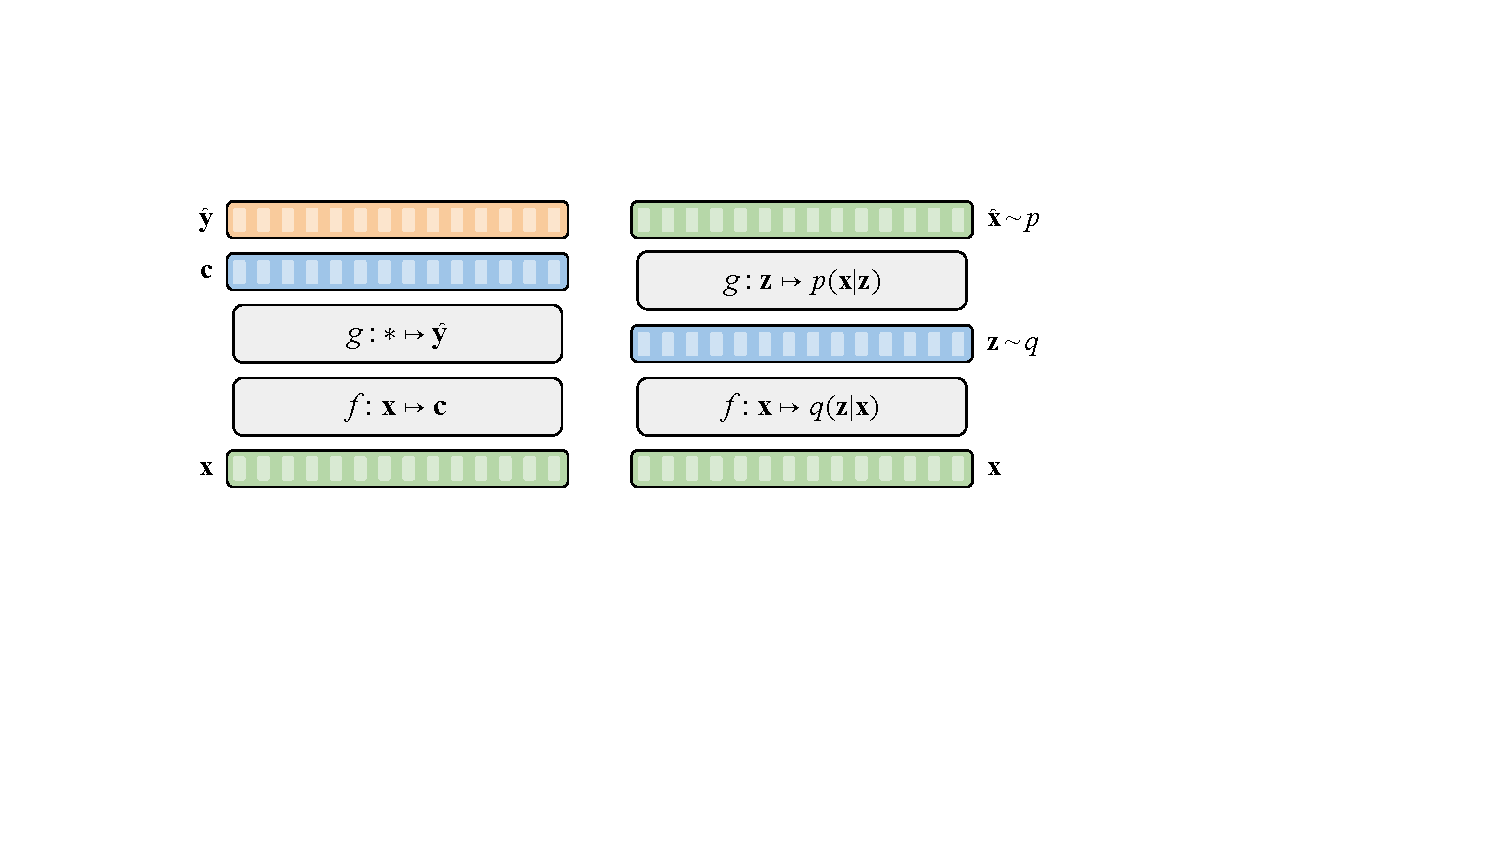
\includegraphics[width=0.90\textwidth]{paper_brief/SSL_LVM.pdf}
    \caption{A schematic overview of the two groups of models covered in this survey. \textit{Left}: A model trained with self-supervised learning. We take these models to consist of two functions $f(\cdot)$ and $g(\cdot)$ (sec.~\ref{ssec:notation}). After pre-training, $f(\cdot)$ is fine-tuned or used for extracting features $\mathbf{c}$. $g(\cdot)$ is an auxiliary function used to accommodate the self-supervised pre-training task. \textit{Right}: A probabilistic latent variable model. In contrast to the self-supervised model, the functions $f(\cdot)$ and $g(\cdot)$ learn the parameters of distributions $q$ and $p$. The latent variable $\mathbf{z}$ is commonly used for representation learning.}
    \label{fig:ssl_lvm}
\end{figure}

\section{Unsupervised representation learning}

In the following, we group previous work into \textit{self-supervised models} and \textit{probabilistic latent variable models}, and take a \emph{model} to comprise a neural architecture and a corresponding learning algorithm. A schematic overview is found in figure \ref{fig:ssl_lvm}. These categories are neither exhaustive nor mutually exclusive, but allow us to focus on the characteristics that have shaped different branches of research. 

With emphasis on recent successes in the field, we cover literature from the last 10 years. While a complete description of all relevant models is not within the scope of this work, we sketch important technicalities when they are particularly descriptive of certain models. We first define our high-level notation and conventions to ease discussion.


%Similarly, $\textbf{a}_{<t}$ denotes a vector-sequence containing all elements prior to step $t$ and $\textbf{a}_{t \in \mathbb{A}}$ is a vector sequence containing elements with index contained in the set $\mathbb{A}$.
%(or a scalar sequence $a_{i:j}$)

%Input to a model is either a spectrogram $\mathbf{x}_{1:T}$ or the raw speech signal $x_{1:L}$ where $L > T$. Commonly $L = T(\frac{S}{100})$ where $S$ is the sample rate of the raw speech signal.

% \IEEEpubidadjcol % related to the IEEEpubid command in the top

\paragraph{Notation} \label{ssec:notation} We use the subscript $i{:}j$ with $i{\leq}j$ to denote a vector sequence $\textbf{a}_{i:j}$ containing elements $\textbf{a}_{i}$ through $\textbf{a}_{j}$. We denote model input as $\mathbf{x}_{1:T}$ which, in practice, might be either a spectrogram or the raw speech signal, but we do not distinguish between the two in notation as it is not essential to understand the models. Also, models commonly downsample the temporal dimension, but again, this is not crucial to understand the models, so we maintain a notation based on a single temporal dimension $t\in\{1,\dots, T\}$.

When discussing self-supervised models, we use $\mathbf{c}_{1:T}$ to denote a contextualized representation. For stochastic latent variable models, we use $\mathbf{z}_{1:T}$ as is customary to the field. 
% The representation at a single time-step, $\mathbf{c}_t$ or $\mathbf{z}_t$, is typically a function of a larger part of the input space than just $\mathbf{x}_t$, in some cases the entire input sequence $\mathbf{x}_{1:T}$.
While some models are frozen and produce representations used as input for downstream tasks (\textbf{\textsc{frz}}, table \ref{tab:model-taxonomy}), others are designed to be fine-tuned (\textbf{\textsc{ftn}}, table \ref{tab:model-taxonomy}). In either case, we use $f(\cdot)$ to denote the model that is used for the downstream task. We use $g(\cdot)$ to denote any auxiliary model components (e.g., for a reconstruction task we might have $g: \mathbf{c}_t \mapsto \hat{\mathbf{x}}_t$). When a model can be naturally subdivided into multiple components, we simply use $f_*(\cdot)$ where $*$ may be any convenient descriptor. Finally, we often use a subscript when defining a loss, $\mathcal{L}_i$, to imply that the total loss is computed as a sum over $i$.


\subsection{Self-supervised models}
\label{sec:ssmodels}

Self-supervised learning is a subset of unsupervised learning \cite{tsai2020self}. Where other unsupervised methods can be seen as a means to an end in itself (e.g., clustering or data generation), self-supervised learning takes the form of a pretext task that only adds value when associated with a downstream task. This makes self-supervised learning tie naturally with semi-supervised learning, but it may also be part of a fully unsupervised setup \cite{baevski2021unsupervised}. Self-supervised learning is often characterized by automatically deriving the target from the input or other unlabeled examples \cite{ouali2020overview}.


\paragraph{Predictive models} Similar to classic autoregressive language models \cite{mikolov2010recurrent}, contextualized speech representations can be learned by predicting future values of a simple representation \cite{oord2018representation, chung2019unsupervised, schneider2019wav2vec, chung2020generative, jiang2021further} (\textbf{\textsc{prd}}, table \ref{tab:model-taxonomy}). Modeling spectrograms directly, autoregressive predictive coding (APC, \citealp{chung2019unsupervised}) is perhaps the simplest example in this category. The forward pass and loss are computed as
\begin{align}
    \mathbf{c}_{t} &= f(\mathbf{x}_{1:t})  \label{eq:apc_f} \\ 
    \hat{\mathbf{x}}_{t+k} &= g(\mathbf{c}_{t}) \\
    %\mathcal{L}_t(\mathbf{\hat{x}}_{t+k}, \mathbf{x}_{t+k}) &= |\mathbf{\hat{x}}_{t+k} - \mathbf{x}_{t+k}|
    \mathcal{L}_t &= \lVert \hat{\mathbf{x}}_{t+k} - \mathbf{x}_{t+k} \rVert_1\enspace.
\end{align}
%
\noindent Here, $f(\cdot)$ and $g(\cdot)$ are parameterized by neural networks such that each $\mathbf{c}_t$ is only conditioned on previous inputs $\mathbf{x}_{1:t}$ and $\hat{\mathbf{x}}_{t+k}$ is computed step-wise. \citet{chung2019unsupervised} use a stack of unidirectional LSTMs for $f(\cdot)$ and a linear regression layer for $g(\cdot)$. Tasks that seek to predict or reconstruct the input are very common. In the literature, these are often jointly referred to as reconstruction tasks (\textbf{\textsc{rec}}, table \ref{tab:model-taxonomy}) \cite{liu2021tera, wang2021unispeech}, although this is somewhat misleading in the case of prediction.

Contrary to generative models, such as WaveNet \cite{oord_wavenet:_2016}, the APC model is not restricted to next-step prediction. Instead, it predicts $k > 0$ steps ahead in order to ensure that the model does not learn a trivial solution by exploiting the smoothness of the signal. Depending on the downstream task, we are often interested in learning so-called slow features that will typically span multiple input frames \cite{wiskott2002slow}. Even the smallest linguistic units of speech, phonemes, tend to span $0.1$ seconds on average \cite{garofolo_timit_1993}, whereas spectrogram frames $\mathbf{x}_t$ are typically computed at $0.01$ second intervals. However, sometimes local smoothness is explicitly used to define the task \cite{badino2014auto, jati2017speaker2vec, jati2019neural}.


%In early work, \citet{badino2014auto} propose a step-wise bottleneck model that learns to predict $\mathbf{x}_{t+1}$ from $\mathbf{x}_{t}$. Since phonetic information changes slowly, $\mathbf{x}_{t+1}$ is argued to be a noisy version of $\mathbf{x}_{t}$ encoding almost the same phonetic content. Thus, the model is akin to a denoising autoencoder.
%A similar idea has been proposed by Jati and Georgiou \cite{jati2019neural} to learn speaker embeddings.

% Next-step prediction has also been frequently used for generative models (\textbf{\textsc{gen}}, table \ref{tab:model-taxonomy}). The popular speech synthesis model WaveNet is perhaps the most obvious example \cite{oord_wavenet:_2016}. While this work does not consider representation learning, the model might learn useful features similar to those learned with APC.


\paragraph{Contrastive models} Speech contains localized noise (e.g., phase shifts) that does not inform slow feature learning. Thus, directly modeling speech might not be the best way to learn contextualized representations. Contrastive predictive coding (CPC,  \citealp{oord2018representation}) targets a local variable $\mathbf{v}_{1:T}$, learned from the model input $\mathbf{x}_{1:T}$, instead of the input itself. The forward pass is
%
\begin{align}
    \mathbf{v}_{t} &= f_{v}(\mathbf{x}_{t-r:t+r}) \label{eq: cpc local representation} \\
    \mathbf{c}_{t} &= f_{c}(\mathbf{v}_{1:t}) \\
    \hat{\mathbf{v}}_{t,k} &= g_k(\mathbf{c}_{t}) \enspace,
    %g_k(\mathbf{c}_{t}, \mathbf{v}_{t+k}) &= \mathbf{v}_{t+k}^{\intercal} \mathbf{W}_k \mathbf{c}_{t}
    %\mathcal{L}_{t,k} &= - \log \left(\frac{g_k(\mathbf{c}_{t}, \mathbf{v}_{t+k})}{\sum_{n \sim \mathcal{D}} g_k(\mathbf{c}_{t}, \mathbf{v}_{n})} \right)
    % \mathcal{L}_{t,k} &= -\log g_k + \log \sum_{n \sim \mathcal{D}} g_k
\end{align}
%
\noindent where $f_v(\cdot)$ is a convolutional neural network, such that each $\mathbf{v}_{t}$ only encodes information from a limited receptive field $2r+1$. Again, $f_c(\cdot)$ should be limited to condition each $\mathbf{c}_t$ on previous time-steps $\mathbf{v}_{1:t}$ and $g_k(\cdot)$ is a step-wise transformation. The loss is based on noise constrastive estimation \cite{gutmann2010noise} and is given by
\begin{align}
    \mathcal{L}_{t,k} &= - \log \left(\frac{\exp(\hat{\mathbf{v}}_{t,k}^{\text{\tiny T}}\mathbf{v}_{t+k})}{\sum_{n \sim \mathcal{D}} \exp(\hat{\mathbf{v}}_{t,k}^{\text{\tiny T}}\mathbf{v}_{n})} \right)\enspace .
    % \mathcal{L}_{t,k} &= - \hat{\mathbf{v}}_{t,k}^{\text{\tiny T}}\mathbf{v}_{t+k} + \log \sum_{n \sim \mathcal{D}} \exp(\hat{\mathbf{v}}_{t,k}^{\text{\tiny T}}\mathbf{v}_{n})\enspace .
    % \mathcal{L}_{t,k} &= -\log g_k + \log \sum_{n \sim \mathcal{D}} g_k
    \label{eq: cpc loss}
\end{align}
%
\noindent Here, $\mathcal{D}$ is a set of indices including the target index $t+k$ and negative samples drawn from a proposal distribution, which is typically taken to be a uniform distribution over the set $\{1,\dots,T\}$. Note that the loss is also indexed by $k$ to show that CPC targets multiple offsets. The APC model is easily extended in a similar way \cite{chung2020improved}.

Crucially, we cannot simply predict $\mathbf{v}_{t+k}$ from $\mathbf{c}_t$ with an $\ell_1$ loss. This would cause $f_v(\cdot)$ to collapse to a trivial solution, such as setting all $\mathbf{v}_t$ equal. With a contrastive loss on the other hand, setting all $\mathbf{v}_t$ equal would cause $\mathcal{L}_{k,t}$ to be constant at a value no better than a random baseline. 

A model closely related to the original CPC model is wav2vec \cite{schneider2019wav2vec}. It uses a different parameterization of the functions $f_v(\cdot)$ and $f_c(\cdot)$, and modifies the loss to consider a binary prediction task, such that we have
%
\begin{align}
    %g_k(\mathbf{c}_{t}, \mathbf{v}_{t+k}) &= \log(\sigma(\mathbf{v}_{t+k}^{\intercal} (\mathbf{W}_k \mathbf{c}_{t} + \mathbf{b}_k)))\\
    \mathcal{L}_{t,k} &= - \log(\sigma(\hat{\mathbf{v}}_{t,k}^{\text{\tiny T}}\mathbf{v}_{t+k})) - \sum_{n \sim \mathcal{D}} \log(\sigma(-\hat{\mathbf{v}}_{t,k}^{\text{\tiny T}}\mathbf{v}_{n})) \,.
    \label{eq: wav2vec loss}
\end{align}

\noindent This model was among the first to show that learned representations can be used to improve end-to-end speech recognition. As we will see, the wav2vec framework has evolved to shape state-of-the-art representation learning for speech.


\paragraph{Masking-based models} One downside of predictive tasks is that models are primarily unidirectional. Some work has extended APC and CPC inspired models with separate encoders operating in opposite directions \cite{ling2020deep, kawakami2020learning, borgholt2021scaling}, but these models are still restricted to process left and right context separately. Inspired by the masked language model task used for text-based representation learning \cite{devlin2019bert}, several papers have used masking to overcome this challenge (\textbf{\textsc{msk}}, table \ref{tab:model-taxonomy}). Masking refers to replacing parts of the input with zeros or a learned masking vector. For zero-masking \cite{jiang2019improving, liu2020mockingjay, wang2020unsupervised, chi2021audio, ling2020decoar}, we have
\begin{align}
    \mathbf{c}_{1:T} &= f(\mathbf{x}_{1:T} \circ \mathbf{m}_{1:T})\\
    \mathbf{\hat{x}}_{t} &= g(\mathbf{c}_{t}) \\
    \mathcal{L}_t &= \lVert \mathbf{\hat{x}}_{t} - \mathbf{x}_{t} \rVert_1\enspace,
\end{align}
where the $\circ$ operator denotes the Hadamard product, $f(\cdot)$ is typically a transformer encoder or a bidirectional recurrent neural network, $g(\cdot)$ is a step-wise transformation, and $\mathbf{m}_{1:T}$ is a mask such that $m_{t,i} \in \{0,1\}$. Alternatively, $\mathbf{m}_{1:T}$ is used to select which $\mathbf{x}_t$ are replaced by a learned masking vector. The entries of $\mathbf{m}_{1:T}$ are determined by some stochastic policy. One frequent inspiration is SpecAugment \cite{park2019specaugment}, which was originally proposed for supervised speech recognition and applies frequency and time masking to spectrogram representations.
While temporal masking is most common, frequency masking has also been adopted for representation learning  \cite{wang2020unsupervised}. A simple, yet popular, masking strategy is to draw a proportion of input indices $t_i\sim\{1,\dots,T-M\}$ without replacement, and then mask $\{t_i, \dots, t_i+M\}$ \cite{baevski2020wav2vec, hsu2021hubert, ling2020decoar}.

Combining masking with a contrastive loss, wav2vec 2.0 was the first work to show that a competitive speech recognition model can be learned by fine-tuning a pre-trained model with as little as 10 minutes of labeled data. For this model
%
\begin{align}
    \mathbf{v}_{t} &= f_v(\mathbf{x}_{t-r:t+r}) \\
    \mathbf{c}_{1:T} &= f_c(\mathbf{v}_{1:T} \circ \mathbf{m}_{1:T}) \\
    \mathbf{q}_t &= g_q(\mathbf{v}_t) \enspace . \label{w2v2 qtz}
\end{align}

\noindent Here, $f_v(\cdot)$ is a convolutional neural network, $f_c(\cdot)$ is a transformer encoder \cite{vaswani2017attention} and $g_q(\cdot)$ is a quantization module used to learn targets from the localized variable $\mathbf{v}_{1:T}$. Computing quantized targets this way requires an extra loss term, which we will present when we discuss quantization in general below. The contrastive loss for wav2vec 2.0 is similar to that of the CPC model,
%
\begin{align}
    \mathcal{L}_t &= - \log \left(\frac{\exp(S_{\text{c}}(\mathbf{c}_{t}, \mathbf{q}_{t}))}{\sum_{n \sim \mathcal{D}} \exp(S_{\text{c}}(\mathbf{c}_{t}, \mathbf{q}_{n}))} \right) \enspace , \label{w2v2 loss}
\end{align}
%
\noindent where $S_{\text{c}}(\cdot)$ is the cosine similarity and the negative samples in $\mathcal{D}$ are sampled from other masked time-steps. 

In general, masking is less data efficient than prediction, as only the masked portion of the input is non-trivial to reconstruct. For this reason, the loss might be computed as
%
\begin{align}
    \mathcal{L}_t &= \lVert (\mathbf{\hat{x}}_{t} - \mathbf{x}_{t}) \circ (\mathbf{1} - \mathbf{m}_t) \rVert_1 \enspace .
\end{align}

\noindent Non-autoregressive predictive coding (NPC, \citealp{liu2020non}) tries to resolve this by using a convolutional neural network where the kernel is masked instead of the input.
%That is, the model is prevented from using $\mathbf{x}_{t}$ for its corresponding reconstruction $\mathbf{\hat{x}}_{t}$.
This allows for complete data utilization, but limits the amount of context encoded in the learned representation.
Figure \ref{fig:ssl_grid} summarizes the models discussed so far.

\begin{figure}[!t]
    \centering
    \setlength\tabcolsep{1.5pt}
    \begin{tabular}{>{\centering\arraybackslash} m{4mm}  >{\centering\arraybackslash} m{0.45\textwidth}|>{\centering\arraybackslash} m{0.45\textwidth}}
          & {\small \textsc{predictive}} & {\small \textsc{masking-based}} \\
        %\midrule
        \rotatebox{90}{{\small \textsc{reconstruct}}} & 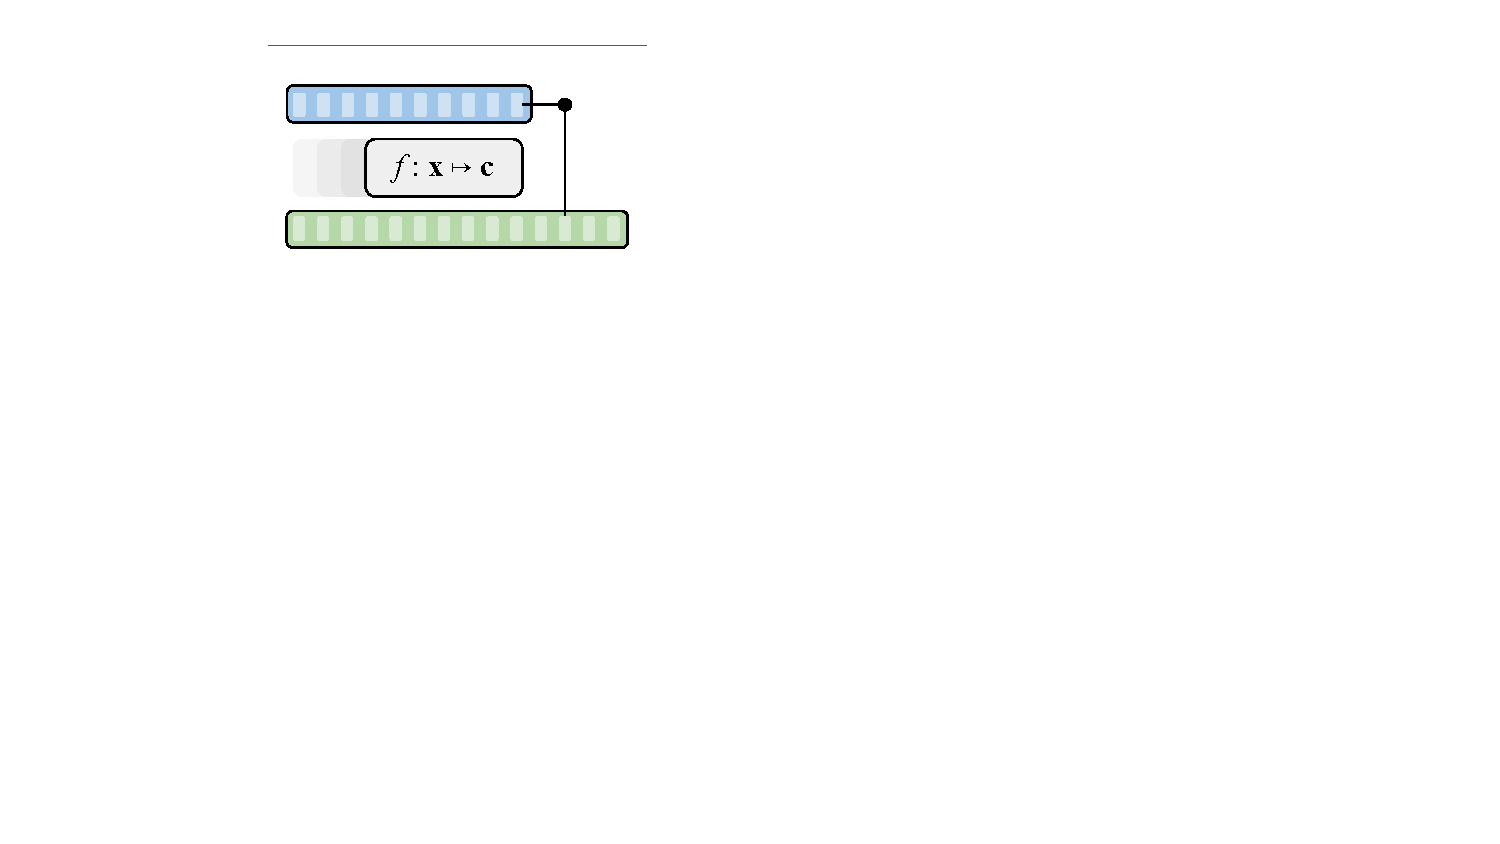
\includegraphics[width=0.45\textwidth]{paper_brief/REC_PRD.pdf} & 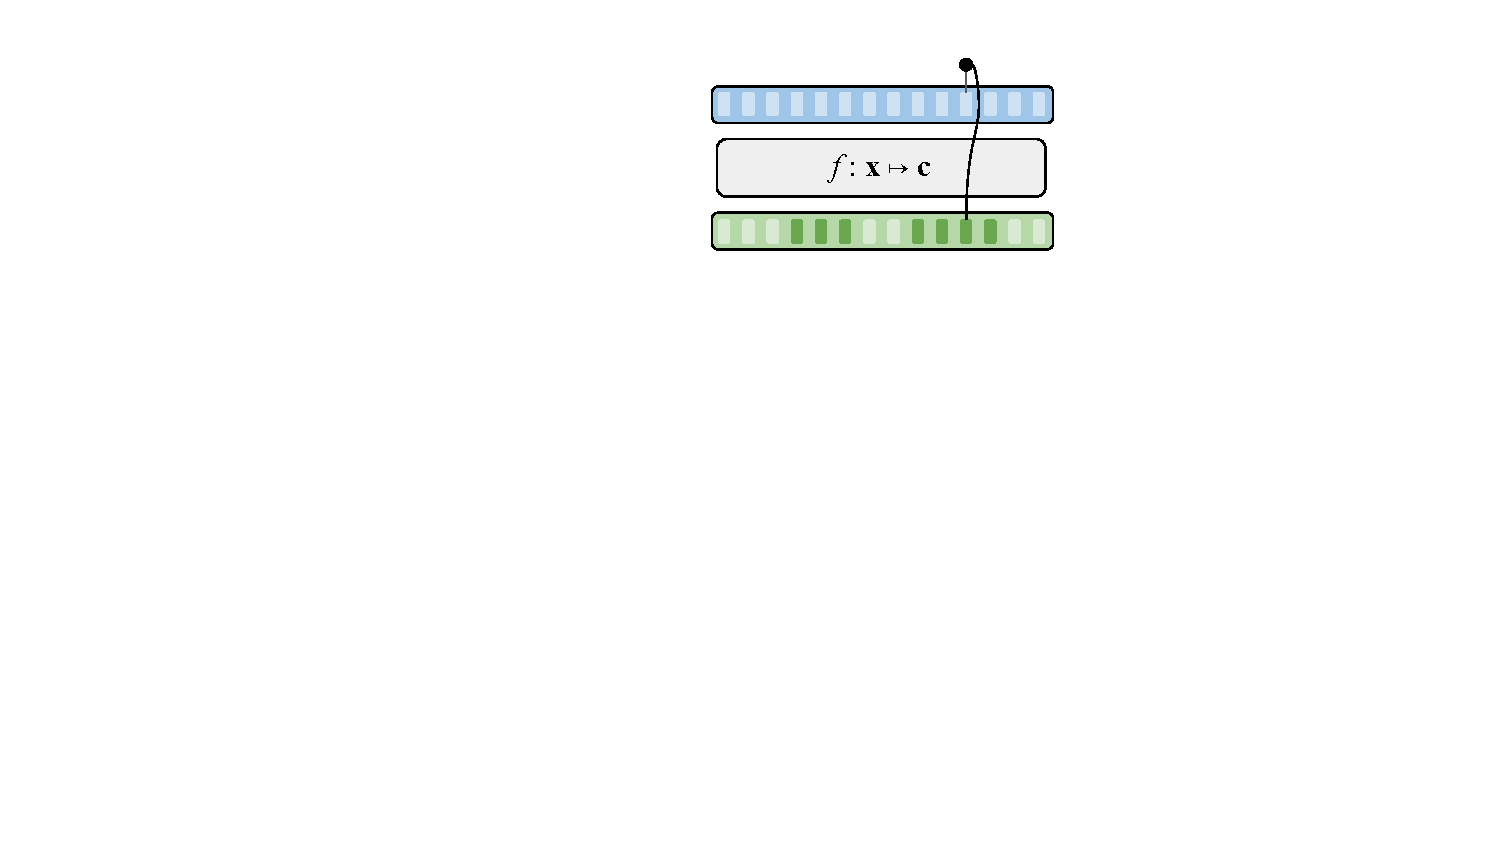
\includegraphics[width=0.45\textwidth]{paper_brief/REC_MSK.pdf}  \\
        \midrule
        \rotatebox{90}{{\small \textsc{contrastive}}} & 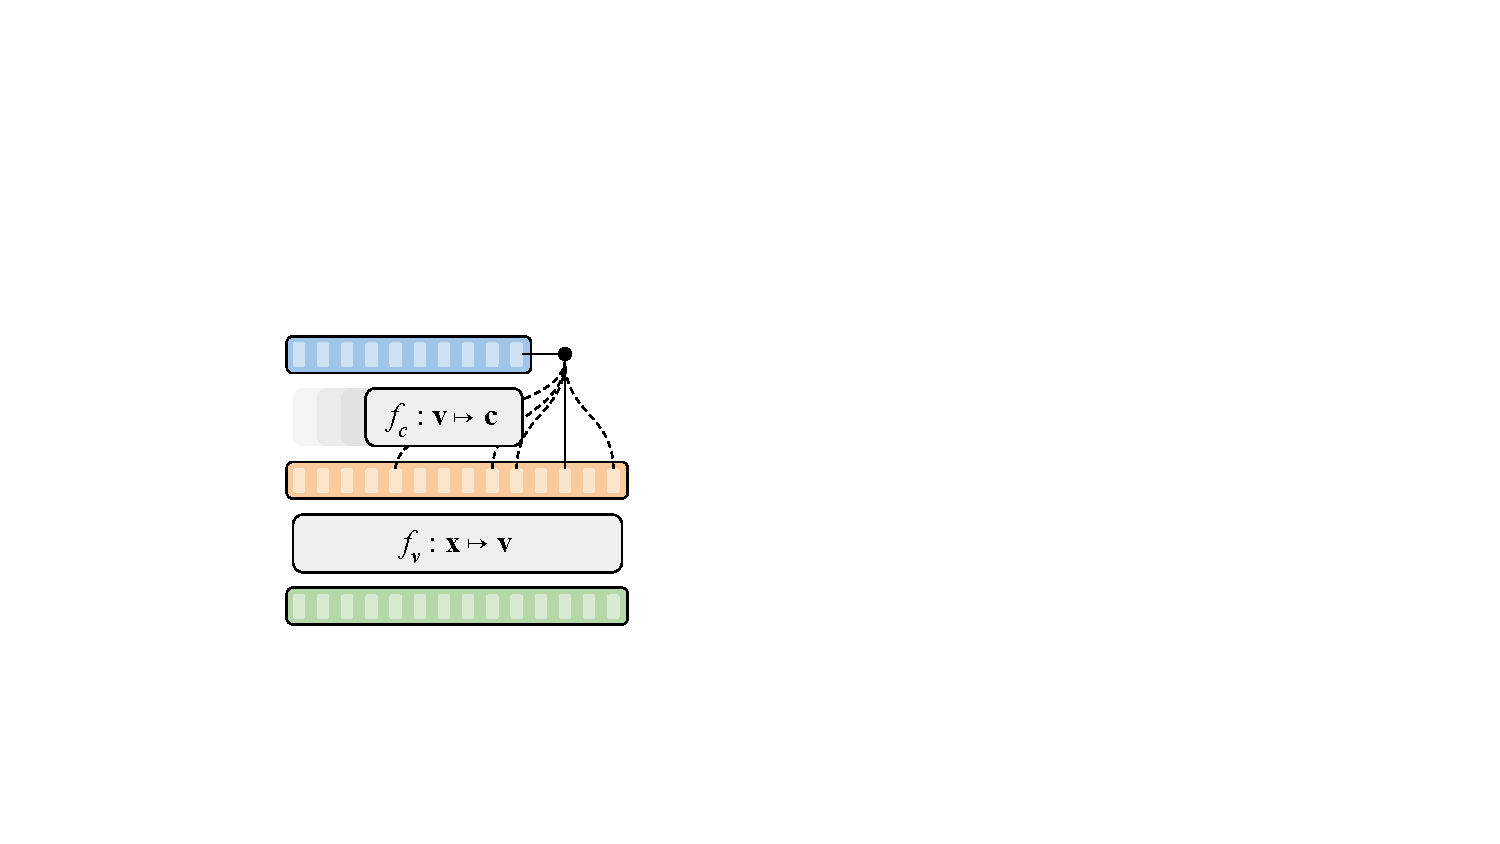
\includegraphics[width=0.45\textwidth]{paper_brief/CON_PRD.pdf} & 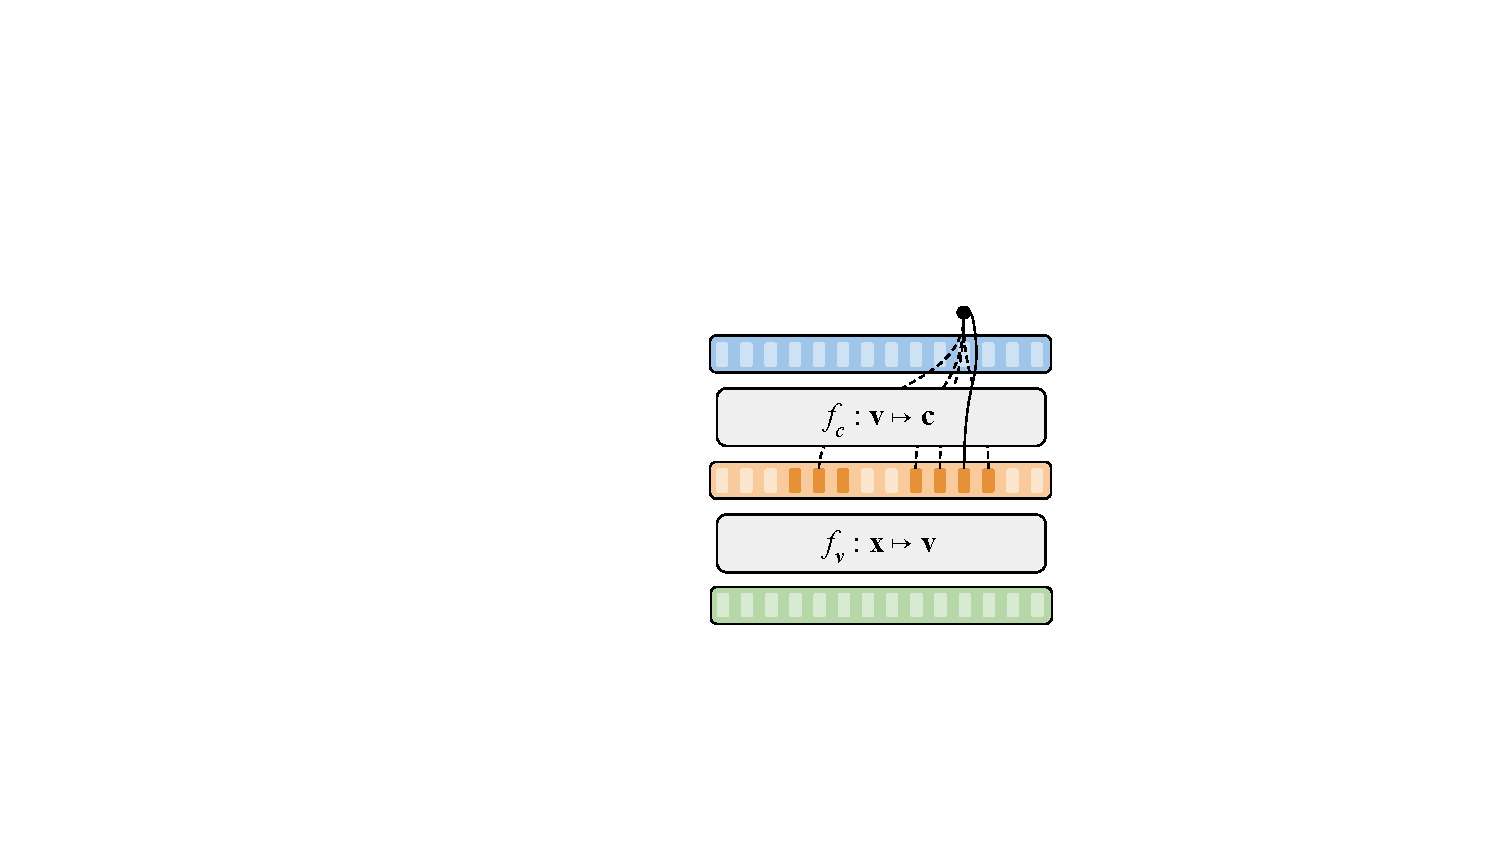
\includegraphics[width=0.45\textwidth]{paper_brief/CON_MSK.pdf}
    \end{tabular}
    \caption{
    Schematic of self-supervised methods. Each subfigure illustrates the loss computation for a single time-step.
    The temporal subscript has been left out for simplicity. 
    %Examples of models in each category include APC (\textbf{\textsc{prd}} + \textbf{\textsc{rec}}), Mockingjay (\textbf{\textsc{msk}} + \textbf{\textsc{rec}}), CPC (\textbf{\textsc{prd}} + \textbf{\textsc{con}}) and wav2vec 2.0 (\textbf{\textsc{msk}} + \textbf{\textsc{con}}).
    }
    \label{fig:ssl_grid}
\end{figure}



\begin{sidewaystable*}[t]
    \caption{Selected models classified according to the binary attributes identified throughout the text. The models are sorted according to first publication date on arXiv which might differ from the citation year. \textbf{\textsc{msk}}: masking, \textbf{\textsc{prd}}: prediction, \textbf{\textsc{con}}: contrastive, \textbf{\textsc{rec}}: reconstruction, \textbf{\textsc{qtz}}: quantization, \textbf{\textsc{gen}}: generative, \textbf{\textsc{frz}}: frozen, \textbf{\textsc{ftn}}: fine-tuned, \textbf{\textsc{loc}}: local, \textbf{\textsc{glo}}: global.}
    \label{tab:model-taxonomy}
    \begin{center}
        \renewcommand{\arraystretch}{1.1}
        \resizebox{0.925\textwidth}{!}{%
        \begin{tabular}{ l l | c c c c c c | c c c | c c } 
            \toprule
            
            \multicolumn{2}{c}{} & 
            \multicolumn{6}{c}{\footnotesize\textsc{Model and task design}} & 
            \multicolumn{3}{c}{\footnotesize\textsc{Resolution}} &
            \multicolumn{2}{c}{\footnotesize\makebox[0pt][c]{\textsc{Usage}}} \\
            \textbf{\textsc{model}} &
            \textbf{\textsc{pub. date}} &
            \textbf{\textsc{msk}} & 
            \textbf{\textsc{prd}} & 
            \textbf{\textsc{con}} &  
            \textbf{\textsc{rec}} &  
            \textbf{\textsc{qtz}} & 
            \textbf{\textsc{gen}} & 
            \textbf{\textsc{loc}} & 
            \textbf{\textsc{glb}} & 
            \textbf{\textsc{var}} & 
            \textbf{\textsc{frz}} & 
            \textbf{\textsc{ftn}} \\
            
            \midrule
            \multicolumn{12}{c}{\textsc{Self-supervised models}} \\
            \midrule
            
            %                                                           MSK      PRD      CON      REC      QTZ      GEN      LOC      GLB     VAR      FRZ      FTN
            \textbf{Audio Word2vec} \footnotesize\cite{chung2016audio}      & 2016 Mar. & \cmark & \xmark & \xmark & \cmark & \xmark & \xmark & \xmark & \cmark & \xmark & \cmark & \xmark \\
            \textbf{Speech2Vec} \footnotesize\cite{chung2018speech2vec}     & 2018 Mar. & \xmark & \cmark & \xmark & \cmark & \xmark & \xmark & \xmark & \cmark & \xmark & \cmark & \xmark \\
            \textbf{Unspeech} \footnotesize\cite{milde2018unspeech}         & 2018 Apr. & \xmark & \cmark & \cmark & \xmark & \xmark & \xmark & \xmark & \cmark & \xmark & \cmark & \xmark \\
            
            \textbf{CPC} (van den Oord et al. 2018)         & 2018 Jul. & \xmark & \cmark & \cmark & \xmark & \xmark & \xmark & \cmark & \xmark & \xmark & \cmark & \xmark \\
            
            %PASE \footnotesize\cite{Pascual2019}                   & 2019 Apr. & \xmark & \xmark & \cmark & \cmark & \xmark & \xmark & \cmark & \xmark & \xmark & \cmark & \cmark \\ % 6/4
            \textbf{APC} \footnotesize\cite{chung2019unsupervised}          & 2019 Oct. & \xmark & \cmark & \xmark & \cmark & \xmark & \xmark & \cmark & \xmark & \xmark & \cmark & \xmark \\ % 5/4
            \textbf{wav2vec} \footnotesize\cite{schneider2019wav2vec}       & 2019 Apr. & \xmark & \cmark & \cmark & \xmark & \xmark & \xmark & \cmark & \xmark & \xmark & \cmark & \xmark \\ % 11/4
            
            %VQ-APC \footnotesize\cite{chung2020vector}             & 2020 May  & \xmark & \cmark & \xmark & \cmark & \cmark & \xmark & \cmark & \xmark & \xmark & \cmark & \xmark \\ 
            
            \textbf{Mockingjay}  \footnotesize\cite{liu2020mockingjay}      & 2019 Oct. & \cmark & \xmark & \xmark & \cmark & \xmark & \xmark & \cmark & \xmark & \xmark & \cmark & \cmark \\ % 25/10-19
            %DeCoAR \footnotesize\cite{ling2020deep}                & 2019 Dec. & \xmark & \cmark & \xmark & \cmark & \xmark & \xmark & \cmark & \xmark & \xmark & \cmark & \xmark \\ % 3/12-19
            %PASE+ \footnotesize\cite{Ravanelli2020}                & 2020 Jan. & \cmark & \xmark & \cmark & \cmark & \xmark & \xmark & \cmark & \xmark & \xmark & \cmark & \cmark \\ % 25/1
            \textbf{wav2vec 2.0} \footnotesize\cite{baevski2020wav2vec}     & 2020 Jun. & \cmark & \xmark & \cmark & \xmark & \cmark & \xmark & \cmark & \xmark & \xmark & \xmark & \cmark \\ % 20/6
            %TERA \footnotesize\cite{liu2021tera}                   & 2021 Jul. & \cmark & \xmark & \xmark & \cmark & \xmark & \xmark & \cmark & \xmark & \xmark & \cmark & \cmark \\ % 12/7
            \textbf{NPC} \footnotesize\cite{liu2020non}                     & 2020 Nov. & \cmark & \xmark & \xmark & \cmark & \cmark & \xmark & \cmark & \xmark & \xmark & \cmark & \xmark \\ % 1/11
            \textbf{DeCoAR 2.0} \footnotesize\cite{ling2020decoar}          & 2020 Dec. & \cmark & \xmark & \xmark & \cmark & \cmark & \xmark & \cmark & \xmark & \xmark & \cmark & \xmark \\ % 11/12
            \textbf{SCPC} \footnotesize\cite{bhati2021segmental}            & 2021 Jun. & \xmark & \cmark & \cmark & \xmark & \xmark & \xmark & \cmark & \xmark & \cmark & \cmark & \xmark \\ % 3/6
            \textbf{HuBERT} \footnotesize\cite{hsu2021hubert}               & 2021 Jun. & \cmark & \xmark & \xmark & \xmark & \cmark & \xmark & \cmark & \xmark & \xmark & \xmark & \cmark \\ % 14/6
            
            
            
            \midrule
            \multicolumn{12}{c}{\textsc{Probabilistic latent variable models}} \\
            \midrule
            %                                                           MSK      PRD      CON      REC      QTZ      GEN      LOC      GLO     VAR      FRZ      FTN
            % Conv. DBN \footnotesize\cite{lee_unsupervised_2009}    & 2009 Jan. & \xmark & \xmark & \xmark & \cmark & \xmark & \cmark & \cmark & \xmark & \cmark & \xmark & \xmark \\
            \textbf{VRNN} \footnotesize\cite{chung_recurrent_2015}          & 2015 Jun. & \xmark & \xmark & \xmark & \cmark & \xmark & \cmark & \cmark & \xmark & \xmark & \cmark & \xmark \\
            \textbf{SRNN} \footnotesize\cite{fraccaro_sequential_2016}      & 2016 May  & \xmark & \xmark & \xmark & \cmark & \xmark & \cmark & \cmark & \xmark & \xmark & \cmark & \xmark \\
            \textbf{HMM-VAE} \footnotesize\cite{ebbers_hidden_2017}         & 2017 Mar. & \xmark & \xmark & \xmark & \cmark & \xmark & \cmark & \cmark & \xmark & \xmark & \cmark & \xmark \\
            \textbf{ConvVAE} \footnotesize\cite{hsu_learning_2017}          & 2017 Apr. & \xmark & \xmark & \xmark & \cmark & \xmark & \cmark & \xmark & \cmark & \xmark & \cmark & \xmark \\
            \textbf{FHVAE} \footnotesize\cite{hsu_unsupervised_2017}        & 2017 Sep. & \xmark & \xmark & \xmark & \cmark & \xmark & \cmark & \cmark & \cmark & \xmark & \cmark & \xmark \\
            \textbf{VQ-VAE} (van den Oord et al. 2018)                      & 2017 Nov. & \xmark & \xmark & \xmark & \cmark & \cmark & \cmark & \cmark & \xmark & \xmark & \cmark & \xmark \\
            \textbf{BHMM-VAE} \footnotesize\cite{glarner_full_2018}         & 2018 Mar. & \xmark & \xmark & \xmark & \cmark & \xmark & \cmark & \cmark & \xmark & \xmark & \cmark & \xmark \\
            \textbf{STCN} \footnotesize\cite{aksan_stcn_2019}               & 2019 Feb. & \xmark & \xmark & \xmark & \cmark & \xmark & \cmark & \cmark & \xmark & \xmark & \cmark & \xmark \\
            \textbf{FDMM} \footnotesize\cite{khurana_factorial_2019}        & 2019 Oct. & \xmark & \xmark & \xmark & \cmark & \xmark & \cmark & \cmark & \cmark & \xmark & \cmark & \xmark \\
            \textbf{ConvDMM} \footnotesize\cite{khurana_convolutional_2020} & 2020 Jun. & \xmark & \xmark & \xmark & \cmark & \xmark & \cmark & \cmark & \xmark & \xmark & \cmark & \xmark \\
            \bottomrule
        \end{tabular}
        }
    \end{center}
\end{sidewaystable*}
    

\paragraph{Quantization} 
Several models enforce a discrete latent space by quantizing the vector representation (\textbf{\textsc{qtz}}, table \ref{tab:model-taxonomy}). The two most popular approaches are the Gumbel-softmax \cite{jang2016categorical, maddison2016concrete} and the quantization used in the VQ-VAE \cite{oord_neural_2018}.

%Several models enforce a discrete latent space by quantizing the vector representation (\textbf{\textsc{qtz}}, table \ref{tab:model-taxonomy}). A popular approach for online vector quantization is to use the Gumbel softmax \cite{jang2016categorical, maddison2016concrete}. This approach corresponds to approximate differentiable sampling from a categorical distribution. Another common approach employs a codebook of learnable representations. This approach was popularized with the VQ-VAE \cite{oord_neural_2018}, and thus, we refer to it as the VQ-VAE approach. Both approaches are non-differentiable and obtain gradients using the straight-through estimator \cite{bengio2013estimating}.

\textit{Gumbel-softmax approach:} 
Say we want to quantize a vector $\mathbf{v}$ such that it takes one of $K$ possible values. We first map $\mathbf{v}$ to $\mathbf{l} \in \mathbb{R}^K$ and then map $\mathbf{l}$ to a probability vector $\mathbf{p} \in \mathbb{R}^K$ via the Gumbel softmax given by
\begin{align}
    p_i &= \frac{\exp(l_i + n_i) / \tau}{\sum_k^K \exp(l_k + n_k) / \tau} 
\end{align}
% for $i=1,\dots,K$. Here $\tau$ is a temperature parameter and $\mathbf{n}\in\mathbb R^K$ is a random vector with $n_i = -\log(-\log(u_i))$ for $u_i \sim \mathcal{U}(0, 1)$. 
% As  $\tau \rightarrow 0$, $\mathbf{p}$ approaches a one-hot vector. The Gumbel noise $\mathbf{n}$ is a practical way to sample from the untempered categorical distribution (i.e., $\tau = 1$). 
% A function $\varphi(\mathbf{p})$ is then used to map $\mathbf{p}$ to a discrete sample which can then be used to obtain the quantized vector (e.g., $\mathbf{q}_t$ in eq.~\ref{w2v2 qtz}) via a codebook lookup. As this function is non-differentiable, we have to rely on the straight-through estimator \cite{bengio2013estimating} which assumes that the Jacobian ${\partial \, \varphi}/{\partial \, \mathbf{p}}$ equals the identity matrix. 
for $i=1,\dots,K$. Here $\tau$ is a temperature parameter and $\mathbf{n}\in\mathbb R^K$ is a random vector with $n_i = -\log(-\log(u_i))$ for $u_i \sim \mathcal{U}(0, 1)$.
As  $\tau \rightarrow 0$, $\mathbf{p}$ approaches a one-hot vector. The Gumbel noise $\mathbf{n}$ is a practical way to sample from the untempered categorical distribution (i.e., $\tau = 1$).
$\mathbf{p}$ is mapped to a one-hot vector using a function $\varphi(\cdot)$, such that $\varphi(\mathbf{p})_i = 1$ if $i = \argmax_j p_j$ and $0$ otherwise. 
As this function is non-differentiable, we must rely on the straight-through gradient estimator \cite{bengio2013estimating} which assumes that the Jacobian ${\partial \, \varphi}/{\partial \, \mathbf{p}}$ equals the identity matrix. 
The one-hot vector can then be used for a codebook lookup to obtain the final quantized vector (e.g., $\mathbf{q}_t$ in eq.~\ref{w2v2 qtz}).

%We choose $\varphi(\cdot)$ to return a one-hot vector with $\varphi(\mathbf{p})_i = 1$ if $i = \argmax_j p_j$ and $0$ otherwise. The one-hot vector can then be used for a codebook lookup. For non-differentiable $\varphi(\cdot)$, the gradient is usually taken to be that of the input to $\varphi(\cdot)$. That is, we use the straight-through estimator and assume during training that the Jacobian ${\partial \, \varphi}/{\partial \, \mathbf{p}}$ equals the identity matrix. 
%\begin{align}
%    %\mathbf{v} &= \mathbf{p} + \textsc{sg}(\varphi(\mathbf{p}) - %\mathbf{p}) \, .
%    \frac{\partial \, \varphi}{\partial \, \mathbf{p}} = \mathbf{I}
%\end{align}
%where $\textsc{sg}(\cdot)$ is the \textit{stop gradient} function; an identity function that blocks the gradient from the input. .

The wav2vec 2.0 quantization module (eq.~\ref{w2v2 qtz}) uses the Gumbel softmax. To ensure utilization of codebook vectors, a diversity loss is added to the task specific loss (eq. \ref{w2v2 loss})
%
\begin{align}
    % \mathcal{L} =  - H(\widetilde{\mathbf{p}}) \frac{1}{K}\enspace,
    \mathcal{L} =  - H(\widetilde{\mathbf{p}}) / K \enspace,
\end{align}
\noindent where $H(\cdot)$ is the entropy and $\widetilde{\mathbf{p}}$ is the untempered version of $\mathbf{p}$ without Gumbel noise.

\textit{VQ-VAE approach:} Instead of directly parameterizing a probability distribution, as in the Gumbel softmax, a vector $\mathbf{v}$ can be quantized by replacing it with the closest codebook vector $\mathbf{e}_k$. Specifically, given a learned codebook $\mathbf{e}\in\mathbb{R}^{K\times D}$, where $K$ is the codebook size and $D$ is the dimensionality of each codebook vector $\mathbf{e}_k$, the quantized representation $\mathbf{q}$ of $\mathbf{v}$ is obtained as,
\begin{align}
    \mathbf{q} = \mathbf{e}_k \ , \enspace \text{where} \enspace k=\arg\min_j \norm{\mathbf{v} - \mathbf{e}_j}_2 \enspace .
\end{align}
As $\arg\min$ is non-differentiable, the straight-through estimator is used as for the Gumbel-softmax. 
% The straight-through estimator defines the gradient of this operation by setting the gradient of $\mathbf{v}$ wrt. to the loss equal to that of $\mathbf{q}$. 
%
% Codebook learning is facilitated by a two-term auxiliary loss similar to classical vector quantization dictionary learning \cite{burton_generalization_1983, soong_vector_1985}. Gradients for the codebook vectors are given solely by a vector quantization term, which moves codebook vectors $\mathbf{e}_k$ closer to the non-quantized vectors $\mathbf{v}$. A so-called commitment term is added to ensure that non-quantized vectors do not grow unboundedly by enforcing the encoder to keep them close to a codebook vector.
%
Codebook learning is facilitated by a two-term auxiliary loss similar to classical vector quantization dictionary learning \cite{burton_generalization_1983, soong_vector_1985}. Gradients for the codebook vectors are given solely by a vector quantization term. A so-called commitment term ensures that non-quantized vectors do not grow unboundedly.
\begin{align}
    \mathcal{L} = \underset{\text{vq}}{\underbrace{\norm{\text{sg}\left[\mathbf{v}\right] - \mathbf{e}}_2^2}} + \underset{\text{commitment}}{\underbrace{\beta\norm{\mathbf{v} - \text{sg}\left[\mathbf{e}\right]}_2^2}} \enspace , \label{eq: vector quantization losses}
\end{align}
where $\text{sg}[\mathbf{x}] = \mathbf{x}$ is the stop-gradient operator with the property $\frac{d}{dx_i}\text{sg}[\mathbf{x}] \equiv 0$ for all $i$ and $\beta$ is a hyperparameter. Although vector quantization was introduced by the VQ-VAE which is, in some ways, a latent variable model, it has been applied to self-supervised methods \cite{niekerk_vector_2020, baevski2019vq}.

%but with variations between individual approaches. The VQ-CPC model \cite{niekerk_vector_2020} quantizes $\mathbf{v}$ in the original CPC (eq.~\ref{eq: cpc local representation}) and augments its loss (eq.~\ref{eq: cpc loss}) by addition of the commitment term in eq.~\ref{eq: vector quantization losses}. Instead of learning the codebook via the VQ term, it is updated as a moving average of $\mathbf{v}$ as initially suggested by \citet{oord_neural_2018}. 
%The vq-wav2vec \cite{baevski2019vq} is defined similarly but adds the full auxiliary loss to the wav2vec loss (eq.~\ref{eq: wav2vec loss}) in place of moving averages.

\textit{Motivation:} Similar to how quantization approaches differ between works, so do the motivations provided for employing them. The vq-wav2vec \cite{baevski2019vq, baevski2019effectiveness} %quantizes $\mathbf{v}_{1:T}$ before feeding them to the context network $f_c(\cdot)$. Here, the motivation is 
learn quantized representations in order to apply natural language processing models, like BERT \cite{devlin2019bert}, afterwards. Other works use quantization for speech segmentation \cite{kamper2020towards, chorowski2019unsupervised} or as a bottleneck in order to ``\textit{limit model capacity}" \cite{chung2020vector, ling2020decoar}.
%Quantized representations have also been used for speech segmentation \cite{kamper2020towards, chorowski2019unsupervised}. 
Finally, \citet{chung2020vector} explore quantization between different layers in the APC model, but find that continuous representations consistently perform better than their quantized counterparts on a downstream phoneme classification task


%They find that applying quantization to the output $\mathbf{c}_{1:T}$ yields the best results on a downstream phoneme classification task. However, the continuous representations consistently perform better than their quantized counterparts.

Given our previous discussion of how it might not be beneficial to model localized noise, quantization in wav2vec 2.0 seems well motivated, as it enforces the target representation $\mathbf{q}_{1:T}$ to discard such noise. Taking this idea further, the HuBERT model \cite{hsu2021hubert} uses offline quantization to learn categorical targets. Initially, spectrogram features are used to learn frame-wise labels with $k$-means clustering. A model similar to wav2vec 2.0, but without online quantization, is then trained to infer labels for masked time-steps. Since quantization is offline, this model does not need to rely on a contrastive loss, but can infer the target class directly. The offline quantization also ensures more stable training, as targets do not change abruptly.


\paragraph{Global representations}
The models covered so far learn representations that maintain a temporal resolution proportional to the input resolution. We say that they learn local representations (\textbf{\textsc{loc}}, table \ref{tab:model-taxonomy}). Now, we cover models that learn global representations (\textbf{\textsc{glb}}, table \ref{tab:model-taxonomy}).
%Apart from this attribute, we find that models that learn global representations rely on many of the same techniques described in the previous sections. %We first give a broad overview, before discussing how they relate to the self-supervised models.


 
Early work on global speech representation learning takes inspiration from the autoencoder framework \cite{kramer1991nonlinear}. \citet{chung2016audio} propose a simple sequence-to-sequence autoencoder for learning acoustic word embeddings:
%
% i/x-vectors here?
\begin{align}
    \mathbf{c} &= f(\mathbf{x}_{1:T}) \\
    \hat{\mathbf{x}}_{1:T} &= g(\mathbf{c}) \enspace , \label{eq:dec-aw2v}
\end{align}

\noindent where $f(\cdot)$ and $g(\cdot)$ are a recurrent neural networks, such that $\mathbf{c}$ is taken to be the hidden state at the last time-step $T$ of $f(\cdot)$ and used as initial hidden state of $g(\cdot)$. 
%where $f(\cdot)$ is a recurrent neural network encoder, such that $\mathbf{c}$ is taken to be the hidden state at the last time-step $T$. The decoder, $g(\cdot)$, is also a recurrent neural network where $\mathbf{c}$ is used to initialize the hidden state.
The authors also propose a denoising autoencoder with masked inputs $f(\mathbf{x}_{1:T} \circ \mathbf{m}_{1:T})$. Similar RNN-based autoencoders have also been explored \cite{kamper2019truly, holzenberger2018learning}.
%
%\begin{align}
%    \mathbf{c} &= f(\mathbf{x}_{1:T} \circ \mathbf{m}_{1:T})
%\end{align}
%

Prior to this work, \citet{kamper2015unsupervised} and \citet{renshaw2015comparison} introduced the \textit{correspondence autoencoder}. This method uses dynamic time warping to align input-target segment pairs extracted with unsupervised term discovery. In more recent work, the need for alignment has been alleviated by adopting the sequence-to-sequence framework \cite{kamper2019truly, jacobs2021acoustic}.

%This method relies on unsupervised term discovery with randomized algorithms \cite{jansen2011efficient} to extract corresponding speech segment pairs for training. Thus, one segment is used as input and the other as reconstruction target. Because the paired segments do not necessarily have the same length, they need to be aligned with dynamic time warping.

% In more recent work, this need has been alleviated by adopting the sequence-to-sequence framework \cite{kamper2019truly, jacobs2021acoustic}.
%Unlike the reconstruction tasks reviewed in the previous sections, models presented here all rely on an $\ell_2$ loss, $\mathcal{L} = \lVert \hat{\mathbf{x}}_{1:T} - \mathbf{x}_{1:T} \rVert_2\enspace$.
%
% \begin{align}
%     \mathcal{L} &= \lVert \hat{\mathbf{x}}_{1:T} - \mathbf{x}_{1:T} \rVert_2\enspace.
% \end{align}

Inspired by the work on semantic word embeddings for text \cite{mikolov2013distributed}, the sequence-to-sequence framework has also been used to implement speech-based versions of the skipgram and continuous bag-of-words models \cite{chung2017learning, chung2018speech2vec}. Given a segment corresponding to a single word $\mathbf{x}_{(n)} = \mathbf{x}_{t_{n}:t_{n+1}}$, the skipgram model is trained to predict neighboring words $\mathbf{x}_{(n + k)}$ where $k\ne0$. That is, instead of a single decoder, as in eq. \ref{eq:dec-aw2v}, the skipgram model employs multiple decoders
%
\begin{align}
    \hat{\mathbf{x}}_{(n + k)} = g_k(\mathbf{c})\enspace.
\end{align}
%
Conversely, the continuous bag-of-words model is trained to predict the target word from the neighboring words, so here multiple encoders sum over several offsets $\mathcal{K}$ to obtain $\mathbf{c}$:
%
\begin{align}
    \mathbf{c} &= \sum_{k\in\mathcal{K}} f_k(\mathbf{x}_{(n + k)}) %\enspace .
    % \mathbf{c} &= \sum_{k\in\mathcal K_n} \mathbf{c}_k
\end{align}
%for different values of $k$.
The sequence-to-sequence models described above rely on speech segments corresponding to words. The segments are obtained by supervised forced alignment, %Thus, since forced alignment requires labeled data, the models might be seen as weakly supervised
but similar models have been explored without this requirement \cite{jati2017speaker2vec, tagliasacchi2020pre}.

Contrastive learning has also been explored for global speech representation learning \citep{milde2018unspeech, jati2019neural, jansen2018unsupervised}. And prior to the widespread adoption of neural networks, \citet{levin2013fixed} explore principal component analysis and Laplacian eigenmaps for learning fixed-sized acoustic embeddings.
%Comparable to the skipgram model described above, \citet{milde2018unspeech} and \citet{jati2019neural} define a binary contrastive task where a target segment is used to predict neighboring segments. 

%For general audio representation learning, \citet{jansen2018unsupervised} explore multiple pre-training tasks using a contrastive triplet loss. And prior to the widespread adoption of neural networks, \citet{levin2013fixed} explore principal component analysis and Laplacian eigenmaps for learning fixed-sized acoustic embeddings.


\paragraph{Other work} Some models learn local representations with a variable temporal resolution that is not proportional to the input resolution (\textbf{\textsc{var}}, table \ref{tab:model-taxonomy}). In practice, this is often achieved implicitly, by learning segment boundaries or by taking repeated quantized values to belong to the same segment \cite{kamper2020towards, chorowski2019unsupervised, michel2017blind, kreuk2020self, wang2017gate, dieleman_variable-rate_2021}. An exception is the recently proposed \emph{segmental contrastive predictive coding} (SCPC, \citealp{bhati2021segmental, bhati2021unsupervised}). With this approach, the model explicitly learns segment boundaries, which are used to downsample the representations during training. The same segmentation strategy has subsequently been applied in other models \cite{cuervo2021contrastive}.

Most of the work presented so far fits neatly into the taxonomy presented in table \ref{tab:model-taxonomy}. One exception is the problem-agnostic speech encoder (PASE, \citealp{Pascual2019, Ravanelli2020}) that combines multiple pre-training tasks. Furthermore, many of the presented models have been successfully applied to other use cases. For instance, wav2vec 2.0 and related models have been applied to learn cross-lingual and multi-lingual representations \cite{riviere2020unsupervised, conneau2020unsupervised, khurana2021magic} and proven well-suited for concurrently learning with labeled data \cite{talnikar2021joint, wang2021unispeech}. %We will discuss the downstream application of self-supervised representations further in section \ref{sec:eval}.


\subsection{Probabilistic latent variable models}
\label{sec:plvms}
Another prominent class of models are probabilistic latent variable models (LVMs). 
Before surveying their application to speech, we briefly review LVMs and their usual specification when applied for representation learning in general. We disregard any specific temporal notation without loss of generality. 
We then introduce the variational autoencoder framework (VAE, \citealp{kingma_auto-encoding_2014}). We focus on different dependency structures between data and learned representations, in contrast to the more practical view on self-supervised models taken above.

\paragraph{LVMs and inference}
Fundamental to LVMs is the assumption that the data is produced by a generative process that involves unobserved stochastic latent variables $\textbf{z}$. 
An LVM aims to model this generative process to enable generation of new data $\mathbf{x}$ (\textbf{\textsc{gen}}, table \ref{tab:model-taxonomy}) and inference of the latent variable associated with a given observed variable $\textbf{x}$. 
For representation learning, the inference of latent variables is of primary interest.
An LVM is defined by the observation model $p(\mathbf{x}|\mathbf{z})$, which defines the relationship between the observed and latent variables, and the prior $p(\mathbf{z})$, which defines the relationship among the latent variables \cite{bartholomew_latent_2011}. 
An LVM models the generative process via the joint observation and prior model $p(\mathbf{x}, \mathbf{z})$ often referred to as the generative model. 
The likelihood of an LVM given an example $\textbf{x}$ can be written as
\begin{equation}
    \log p(\mathbf{x}) = \log \int p(\mathbf{x}|\mathbf{z}) p(\mathbf{z}) \,\text{d}\mathbf{z} \enspace.
    \label{eq: lvm log-likelihood}
\end{equation}
The latent variable can be inferred with e.g. Markov Chain Monte Carlo (MCMC) methods \cite{mohamed_monte_2019} or variational inference \cite{jordan_introduction_1999}.

For representation learning, LVMs are commonly defined using the VAE framework \cite{kingma_auto-encoding_2014, rezende_stochastic_2014}) which is also the focus of our exposition. 
In the VAE framework, the observation model $p(\mathbf{x}|\mathbf{z})$ is parameterized using a deep neural network. This choice allows modeling complex and high-dimensional data but also makes the integral in eq.~\ref{eq: lvm log-likelihood} analytically intractable. MCMC methods can be used to estimate it and the true model posterior $p(\mathbf{z}|\mathbf{x})$, but these methods are usually computationally expensive in this setting \cite{mohamed_monte_2019}. 
To counter this and make gradient-based maximum likelihood training feasible, the VAE instead employs variational inference \cite{jordan_introduction_1999}. It approximates the intractable true model posterior by introducing a variational posterior distribution $q(\mathbf{z}|\mathbf{x})$, also parameterized by a deep neural network. From eq.~\ref{eq: lvm log-likelihood}, via Jensen's inequality, this gives rise to a variational lower bound on the likelihood, also known as the evidence lower bound (ELBO).
\begin{equation}
    \log p(\mathbf{x}) \geq \int q(\mathbf{z}|\mathbf{x}) \log \frac{p(\mathbf{x}| \mathbf{z})p(\mathbf{z})}{q(\mathbf{z}|\mathbf{x})} \,\text{d}\mathbf{z} \equiv \mathcal{L}_{\text{ELBO}} \enspace . \label{eq: lvm likelihood bound (elbo)}
\end{equation}
The bound can be efficiently evaluated and optimized with Monte Carlo (MC) estimation by sampling from $q(\mathbf{z}|\mathbf{x})$. Low-variance gradient estimates are usually obtained via reparameterization of $q(\mathbf{z}|\mathbf{x})$ \cite{kingma_auto-encoding_2014} although alternatives exist (e.g., inverse CDF sampling) \cite{mohamed_monte_2019}. 
The ELBO can also be written as
\begin{equation}
    \mathcal{L}_{\text{ELBO}} = \mathbb{E}_{q(\mathbf{z}|\mathbf{x})}\left[ \log p(\mathbf{x}|\mathbf{z}) \right] - D_\text{KL}\left( q(\mathbf{z}|\mathbf{x}) || p(\mathbf{z}) \right) \enspace  \label{eq: lvm likelihood bound recon/kl form (elbo)},
\end{equation}
where $\mathbb{E}\left[ \log p(\mathbf{x}|\mathbf{z}) \right]$ can be seen as a reconstruction loss and $D_\text{KL}\left( q(\mathbf{z}|\mathbf{x})||p(\mathbf{z}) \right)$ is the Kullback-Leibler (KL) divergence between the variational posterior distribution and the prior.

In brief, LVMs of the VAE-type consist of a approximate posterior, $q(\mathbf{z}|\mathbf{x})$, an observation model, $p(\mathbf{x}|\mathbf{z})$, and a prior, $p(\mathbf{z})$. 
% The joint observation model and prior form the generative model which can be efficiently sampled with ancestral sampling which entails first sampling a latent variable $\tilde{\mathbf{z}}\sim p(\mathbf{z})$ followed by sampling the observed variable conditioned on that latent variable, $\tilde{\mathbf{x}}\sim p(\mathbf{x}|\tilde{\mathbf{z}})$. 
With reference to probabilistic coding theory, the approximate posterior is often referred to as the encoder and the observation model as the decoder \cite{kingma_auto-encoding_2014, rezende_stochastic_2014}. From a theoretical perspective, the encoder exists solely as the result of choosing to use variational inference to train the decoder rather than e.g. MCMC. As such, it is also referred to as the inference model. However, from a representation learning perspective, the encoder is essential as it can be used to efficiently obtain the representation $\mathbf{z}$ commonly used for downstream tasks. 
It is still possible to evaluate and sample the true posterior distribution $p(\mathbf{z}|\mathbf{x})$ by applying MCMC methods such as Hamiltonian Monte Carlo on the decoder, but for computational reasons this is rarely done in practice. 

\begin{table}[t!]
\caption{
A comprehensive overview of observation, prior and inference models for VAE type latent variable models with a single latent variable. 
The observation, prior and inference models may all belong to one or more of the categories listed under them as detailed in section \ref{sec:plvms}. 
The types listed here serve as primitives from which more complex structures can be constructed including models with hierarchies of multiple latent variables. 
% We indicate autoregressiveness (\textbf{\textsc{arx}} and \textbf{\textsc{arz}}) using a ``catch-all" notation $*$, e.g. $\mathbf{x}_{*:t-1}$. 
% This serves to indicate that autoregressive dependencies can have different span including at the extremes the full sequence $\mathbf{x}_{1:t-1}$ and the last value $\mathbf{x}_{t-1}$.
% We have not explicitly listed any cases with multiple latent variables as these generally include a multitude of potential dependency structures.
% We outline notable examples of models with hierarchies of latent variables in section \ref{sec:plvms}.
}
\label{tab:lvm-model-primitives}
\begin{center}
    % \renewcommand{\arraystretch}{1.1}
    % \resizebox{0.8\columnwidth}{!}{%
    \begin{tabular}{ l l l } 
        \toprule
        \multicolumn{2}{l}{\textbf{\textsc{Type}}} & \textbf{\textsc{Form}} \\
        \midrule
        \multicolumn{3}{c}{\textsc{Observation model}} \\
        \midrule
        \textbf{\textsc{arx}} & Autoregressive on $\mathbf{x}_t$      & $p(\mathbf{x}_t|\mathbf{x}_{1:t-1})$ \\
        \textbf{\textsc{loc}} & Local latent variable                 & $p(\mathbf{x}_{t}|\mathbf{z}_{1:t})$ \\
        \textbf{\textsc{glb}} & Global latent variable                & $p(\mathbf{x}_{t}|\mathbf{z})$ \\
        \midrule
        \multicolumn{3}{c}{\textsc{Prior}} \\
        \midrule
        % \textbf{\textsc{aut}} & Autoregressive on $\mathbf{z}_t$      & $p(\mathbf{z}_t|\mathbf{z}_{1:t-1})$ \\
        % \textbf{\textsc{obs}} & Observation dependent                                & $p(\mathbf{z}_t|\mathbf{x}_{1:t-1})$ \\
        \textbf{\textsc{arx}} & Autoregressive on $\mathbf{x}_t$      & $p(\mathbf{z}_t|\mathbf{x}_{1:t-1})$ \\
        \textbf{\textsc{arz}} & Autoregressive on $\mathbf{z}_t$      & $p(\mathbf{z}_t|\mathbf{z}_{1:t-1})$ \\
        \textbf{\textsc{ind}} & Locally independent $\mathbf{z}_t$                 & $p(\mathbf{z}_t)$ \\
        \textbf{\textsc{glb}} & Global latent variable                & $p(\mathbf{z})$ \\
        \midrule
        \multicolumn{3}{c}{\textsc{Inference model}} \\
        \midrule
        \textbf{\textsc{arz}} & Autoregressive on $\mathbf{z}_t$      & $q(\mathbf{z}_t|\mathbf{z}_{1:t-1})$ \\
        \textbf{\textsc{flt}} & Filtering                             & $q(\mathbf{z}_t|\mathbf{x}_{1:t})$ \\
        \textbf{\textsc{lsm}} & Local smoothing                       & $q(\mathbf{z}_t|\mathbf{x}_{t-r:t+r})$ \\
        \textbf{\textsc{gsm}} & Global smoothing                      & $q(\mathbf{z}_t|\mathbf{x}_{1:T})$ \\
        \textbf{\textsc{glb}} & Global latent variable                & $q(\mathbf{z}|\mathbf{x}_{1:T})$ \\
        \bottomrule
    \end{tabular}
    % }
    \end{center}
\end{table}

\begin{sidewaystable*}[t]
    \caption{
    Selected latent variable models classified according the attributes defined throughout section \ref{sec:plvms}.
    %The models are sorted according to the publication date of the first version on arXiv which might differ from the year indicated by the citation. 
    %This table supplements the classification provided in table \ref{tab:model-taxonomy} which uses binary attributes largely defined for self-supervised methods. 
    See table~\ref{tab:lvm-model-primitives} for the probability distributions that correspond to each of the attribute short-hands. \textbf{\textsc{hie}} indicates a hierarchical representation.
    %The mathematical expressions of the observation, prior and inference models for the models considered here can be found in table~\ref{tab:lvm-mathematical-expressions}. 
    %Figure~\ref{fig:lvm-graphical-models} depicts corresponding graphical model for selected LVMs of this table.
    }
    \label{tab:lvm-taxonomy}
    \begin{center}
        \renewcommand{\arraystretch}{1.1}
        \resizebox{0.99\textwidth}{!}{% <------ Don't forget this %
        \begin{tabular}{ l l | c c c | c c c c | c c c c c | c } 
            \toprule
            \multicolumn{2}{c}{} & 
            \multicolumn{3}{c}{\footnotesize\textsc{Observation}} & 
            \multicolumn{4}{c}{\footnotesize\textsc{Prior}} & 
            \multicolumn{5}{c}{\footnotesize\textsc{Inference}} \\
            \textbf{\textsc{model}} & 
            \textbf{\textsc{pub. date}} &
            \textbf{\textsc{arx}} & 
            \textbf{\textsc{loc}} & 
            \textbf{\textsc{glb}} &  
            \textbf{\textsc{arx}} & 
            \textbf{\textsc{arz}} & 
            \textbf{\textsc{ind}} & 
            \textbf{\textsc{glb}} &  
            \textbf{\textsc{arz}} & 
            \textbf{\textsc{flt}} & 
            \textbf{\textsc{lsm}} & 
            \textbf{\textsc{gsm}} & 
            \textbf{\textsc{glb}} &
            \textbf{\textsc{hie}} \\
            \midrule
            %                                                              OBSERVATION       |              PRIOR                |                  INFERENCE       
            %                                                         ARX      LOC      GLB      ARX      ARZ     IND      GLB      ARZ      FLT      LSM      GSM      GLB

            % Conv. DBN \cite{lee_unsupervised_2009}    & 2009 Jan. & \xmark & \cmark & \xmark & \xmark & \xmark & \cmark & \xmark & \xmark & \xmark & \xmark & \xmark & \xmark & \xmark \\
            \textbf{VRNN} \footnotesize\cite{chung_recurrent_2015}          & 2015 Jun. & \cmark & \cmark & \xmark & \cmark & \cmark & \xmark & \xmark & \cmark & \cmark & \xmark & \xmark & \xmark & \xmark \\
            \textbf{SRNN} \footnotesize\cite{fraccaro_sequential_2016}      & 2016 May  & \cmark & \cmark & \xmark & \cmark & \cmark & \xmark & \xmark & \cmark & \xmark & \xmark & \cmark & \xmark & \xmark \\
            \textbf{HMM-VAE} \footnotesize\cite{ebbers_hidden_2017}         & 2017 Mar. & \xmark & \cmark & \xmark & \xmark & \cmark & \xmark & \xmark & \cmark & \cmark & \xmark & \xmark & \xmark & \cmark \\
            \textbf{ConvVAE} \footnotesize\cite{hsu_learning_2017}          & 2017 Apr. & \xmark & \xmark & \cmark & \xmark & \xmark & \xmark & \cmark & \xmark & \xmark & \xmark & \cmark & \cmark & \xmark \\
            \textbf{FHVAE} \footnotesize\cite{hsu_unsupervised_2017}        & 2017 Sep. & \xmark & \cmark & \cmark & \xmark & \xmark & \cmark & \cmark & \xmark & \xmark & \xmark & \cmark & \cmark & \cmark \\
            \textbf{VQ-VAE} (van den Oord et al. 2018)            & 2017 Nov. & \cmark & \cmark & \xmark & \xmark & \xmark & \cmark & \xmark & \xmark & \xmark & \cmark & \xmark & \xmark & \xmark \\
            \textbf{BHMM-VAE} \footnotesize\cite{glarner_full_2018}         & 2018 Mar. & \xmark & \cmark & \xmark & \xmark & \cmark & \xmark & \xmark & \cmark & \cmark & \xmark & \xmark & \xmark & \xmark \\
            \textbf{STCN} \footnotesize\cite{aksan_stcn_2019}               & 2019 Feb. & \xmark & \cmark & \xmark & \cmark & \xmark & \xmark & \xmark & \xmark & \cmark & \xmark & \xmark & \xmark & \cmark \\
            \textbf{FDMM} \footnotesize\cite{khurana_factorial_2019}        & 2019 Oct. & \xmark & \cmark & \cmark & \xmark & \cmark & \xmark & \cmark & \cmark & \cmark & \xmark & \xmark & \cmark & \cmark \\
            \textbf{ConvDMM} \footnotesize\cite{khurana_convolutional_2020} & 2020 Jun. & \xmark & \cmark & \xmark & \xmark & \cmark & \xmark & \xmark & \cmark & \xmark & \cmark & \xmark & \xmark & \xmark \\
            % WaveNet AE        &  \\
            % HMM-VAE           &  \\
            % Convolutional DBN &  \\
            \bottomrule
        \end{tabular}
        }
    \end{center}
\end{sidewaystable*}



We next review VAEs applied to speech. We consider the choices of observation, prior and inference models.
% and introduce attributes throughout the text. An overview of these is found in table~\ref{tab:lvm-model-primitives}.
We provide a model taxonomy for selected LVMs in table~\ref{tab:lvm-taxonomy}.
% Supplementing the binary attributes, table~\ref{tab:lvm-mathematical-expressions} explicitly details the observation, prior and inference models of the same selection of LVMs considered in table~\ref{tab:lvm-taxonomy}. 




\paragraph{Observation models} 
A common choice for the observation model $p(\mathbf{x}|\mathbf{z})$ is to include an autoregressive dependency on the observed variable (\textbf{\textsc{arx}}, table \ref{tab:lvm-model-primitives}) that is, $p(\mathbf{x}_t|\mathbf{x}_{1:t-1}, \cdot)$ where $\cdot$ represents some dependency on the latent variable \cite{chung_recurrent_2015, fraccaro_sequential_2016, oord_neural_2018, oord2018representation}. This allows the latent representation to focus on correlations that cannot easily be predicted from the observed variable at previous time-steps \cite{oord2018representation}. In practice, the dependency on $\mathbf{x}_{1:t-1}$ is often assumed to be Markovian and hence only on $\mathbf{x}_{t-1}$. Another common choice is to depend on a local window $\mathbf{x}_{t-r:t-1}$ where $r>1$ is an integer denoting some receptive field. We will take a dependency on $\mathbf{x}_{1:t-1}$ to mean any one of these choices unless otherwise specified.

While the autoregressive dependency might be important for learning a powerful generative model, it might not benefit the learned latent representations. Specifically encouraging the latent representation to discard correlations across the temporal dimension might degrade the quality of the latent representation.
Furthermore, since such a decoder can perform quite well by simply solving an autoregressive prediction problem, similar to WaveNet \cite{oord_wavenet:_2016}, it can make the model prone to suffer from posterior collapse. This problem arises when the approximate and true posterior distributions collapse into the prior which renders the representations non-informative \cite{bowman_generating_2016, sonderby_ladder_2016}. Notably, posterior collapse is a local minimum of the ELBO since the KL-divergence becomes zero. 
Some works alleviate this problem with tricks like KL-annealing and free bits \cite{bowman_generating_2016, sonderby_ladder_2016, kingma_improved_2016}. 
%KL-annealing down-weighs the KL-divergence in the ELBO (eq.~\ref{eq: lvm likelihood bound recon/kl form (elbo)}) gradually phasing it in during an initial training phase \cite{bowman_generating_2016, sonderby_ladder_2016}. Free bits simply returns a zero gradient for KL-divergences smaller than some number. \cite{kingma_improved_2016}. 
The VQ-VAE uses a quantized latent space that is not susceptible to posterior collapse \textit{per se} \cite{oord_neural_2018}. How to equip LVMs with powerful decoders while avoiding posterior collapse is an open problem.

Some LVMs do not use autoregressive observation models \cite{ebbers_hidden_2017, glarner_full_2018, hsu_unsupervised_2017, hsu_learning_2017, khurana_factorial_2019, khurana_convolutional_2020}. These more closely follow the assumption of \emph{local independence} which states that observed variables are conditionally independent given the local (\textbf{\textsc{loc}}, table \ref{tab:lvm-model-primitives}) and/or global (\textbf{\textsc{glb}}, table \ref{tab:lvm-model-primitives}) latent variables \cite{bartholomew_latent_2011}. 
However, this forces the latent variable to encode details about the observed variable to achieve a good reconstruction. This is opposite to contrastive self-supervised learning which allows models to discard details in $\mathbf{x}_{1:T}$ that do not inform the training objective \cite{baevski2020wav2vec}.



\paragraph{Priors}
Priors can be said to belong to one or more of four broad categories. See table~\ref{tab:lvm-model-primitives}. 
% Autoregressive dependency on the observed variable (\textbf{\textsc{arx}}, table \ref{tab:lvm-model-primitives}), autoregressive dependency on the latent variable (\textbf{\textsc{arz}}, table \ref{tab:lvm-model-primitives}), locally independent (\textbf{\textsc{ind}}, table \ref{tab:lvm-model-primitives}) and global (\textbf{\textsc{glb}}, table \ref{tab:lvm-model-primitives}).
Priors that are autoregressive on the observed variable (\textbf{\textsc{arx}}, table \ref{tab:lvm-model-primitives}) take the form $p(\mathbf{z}_t|\mathbf{x}_{1:t-1})$. This generally results in a slow-down of the generative process which may be of concern if the use-case is data generation. %It is also interesting to note that this encourages the latent variables to model less dynamic behaviour in their stochastic transitions and instead rely more on the observed variable. 
Priors that are autoregressive on the latent variable (\textbf{\textsc{arz}}, table \ref{tab:lvm-model-primitives}) take the form $p(\mathbf{z}_t|\mathbf{z}_{1:t-1})$ and enable stochastic temporal transitions similar to hidden Markov models but with potentially nonlinear transition functions \cite{chung_recurrent_2015, fraccaro_sequential_2016, khurana_factorial_2019, khurana_convolutional_2020}.
Locally independent priors (\textbf{\textsc{ind}}, table \ref{tab:lvm-model-primitives}) are rarely applied to sequential latent variables since they make the prior latent dynamics independent of the value of previous latent variables. Models that do impose such priors on sequential latents are quite limited in their generative power, unless they learn the prior dynamics post-hoc as done in the VQ-VAE \cite{oord_neural_2018}. 
Global latent variables (\textbf{\textsc{glb}}, table \ref{tab:lvm-model-primitives}) are fundamentally limited in the amount of information they can encode. Hence, models usually use them in combination with another local latent variable, or to encode fixed length input segments \cite{khurana_factorial_2019, hsu_learning_2017, hsu_unsupervised_2017}.

% Many LVMs have priors that do not have autoregressive dependence on the observed variable (table \ref{tab:lvm-model-primitives}). This allows generating the latent sequence in full before generating the observed sequence. It also permits conditioning past observed variables on future latent variables. Despite this, it is usual to let $\mathbf{x}_t$ depend causally on $\mathbf{z}_{1:t}$ in the generative model. To our knowledge, so far no work has examined full (non-causal) dependence of $\mathbf{x}_{1:T}$ on $\mathbf{z}_{1:T}$ during generation.% where, for example, $\mathbf{z}_T$ can influence $\mathbf{x}_1$. 


\paragraph{Inference models} 
LVMs based on the VAE perform so-called amortized variational inference. Here, a single inference network is used to infer the latent variables of any $\mathbf{x}$. 
For this reason, all inference models covered here are conditioned on the observed sequence in some way. Generally, the inference model can be seen as solving either a filtering or smoothing problem.
In filtering (\textbf{\textsc{flt}}, table \ref{tab:lvm-model-primitives}), the latent variables are assumed to depend only on past and current values of the observed variable, $q(\mathbf{z}_t|\mathbf{x}_{1:t})$ \cite{chung_recurrent_2015, khurana_convolutional_2020}. In global smoothing (\textbf{\textsc{gsm}}, table \ref{tab:lvm-model-primitives}), this causal dependency is replaced with a dependency on all observed values, $q(\mathbf{z}_t|\mathbf{x}_{1:T})$ \cite{fraccaro_sequential_2016, hsu_learning_2017}. 
Smoothing can also be done locally (\textbf{\textsc{lsm}}, table \ref{tab:lvm-model-primitives}), where the latent variables then depend on $\mathbf{x}_{t-r:t+r}$ for some integer $r>0$ \cite{oord_neural_2018}. Compared to self-supervised models that often use transformer encoders it can be hypothesized that global smoothing offers a stronger case than local smoothing and filtering for representation learning.

The inference model may also be used to infer a global latent variable (\textbf{\textsc{glb}}, table \ref{tab:lvm-model-primitives}) that might encode global information about $\mathbf{x}$. 
While it must be included in the prior model it might not be in the observation model, if the model also has a local latent variable. 
Finally, latent variables are often made to depend autoregressively on past inferred values, e.g. $q(\mathbf{z}_t|\mathbf{z}_{1:t-1},\mathbf{x}_{1:t})$ (\textbf{\textsc{arz}}, table \ref{tab:lvm-model-primitives}) \cite{chung_recurrent_2015, fraccaro_sequential_2016}.
% Finally, latent variables are often made to depend autoregressively on past values, $q(\mathbf{z}_t|\mathbf{z}_{1:t-1},\mathbf{x}_{1:t})$ for filtering and $q(\mathbf{z}_t|\mathbf{z}_{1:t-1},\mathbf{x}_{1:T})$ for smoothing (\textbf{\textsc{arz}}, table \ref{tab:lvm-model-primitives}) \cite{chung_recurrent_2015, fraccaro_sequential_2016}.
%Such autoregressive dependencies help the inference model better match the prior dynamics but notably are not employed in models that learn the prior dynamics post-hoc \cite{oord_neural_2018}.


\paragraph{Multiscale and hierarchical models} Some work has explored using a hierarchy of latent variables (\textbf{\textsc{hie}}, table \ref{tab:lvm-taxonomy}). This allows encoding the inductive bias that speech contains information at different temporal scales by letting the latent variables operate at different temporal scales \cite{hsu_unsupervised_2017}. \citet{khurana_factorial_2019} propose using a temporal latent variable along with a global latent variable. 
Recent work has focused on learning a deeper latent hierarchy with five latent variables \cite{aksan_stcn_2019}. 
%Here, the latents have no autoregressive temporal dependencies but instead depend on latent variables further up in the hierarchy with all latent variables operating at the same temporal scale. 
%Interestingly, this effort within LVMs towards separating learned features into representations at different time scales or learning hierarchical representations stands in contrast to work on self-supervised learning where focus is either on learning local or global representations.


\paragraph{Other work}
% Most recent works learn latent variable models via amortized variational inference as introduced by the VAE framework \cite{kingma_auto-encoding_2014, rezende_stochastic_2014}. 
Before the introduction of the VAE, models such as deep belief networks (DBN, \citealp{hinton_fast_2006}) built from stacks of restricted Boltzmann machines \cite{smolensky_parallel_1987,fischer:13} were popular. \citet{lee_unsupervised_2009} show the feasibility of using a two-layered DBN for discovering acoustic units of speech, while \citet{deng_binary_2010} show that a DBN can learn a binary coding of spectrograms that has higher signal-to-noise ratio than classical vector-quantization techniques for speech coding.
DBNs are however notoriously tricky to optimize requiring the use of expensive MCMC sampling techniques for inference or resort to biased gradient estimates \cite{hinton_practical_2012,fischer:10c}.
Non-neural LVMs for speech representation learning have also been explored
\cite{lee_nonparametric_2012, ondel_variational_2016, heck_feature_2017, jansen_weak_2013}.

% Non-neural approaches include Bayesian non-parametric models which can be used for unsupervised acoustic unit discovery. This is often done using a Dirichlet process prior which has the appealing property of automatically inferring the number of acoustic units \cite{lee_nonparametric_2012, ondel_variational_2016, heck_feature_2017}. 
% Finally, Gaussian mixture models have been used to form so-called universal background models from which acoustic representations can be extracted \cite{jansen_weak_2013}.



\section{Discussion}
\label{sec:mtax}
%Throughout the text we defined several binary attributes which are used to characterize a selection of models in table \ref{tab:model-taxonomy} and \ref{tab:lvm-taxonomy}. We discuss representation learning models based on this overarching model taxonomy below.


%In table \ref{tab:model-taxonomy}, we use those derived from the self-supervised models to characterize a selection of models within the two surveyed categories. To obtain a more detailed understanding of the LVMs, we also derived a set of variable dependencies  presented  in table \ref{tab:lvm-model-primitives}. In table \ref{tab:lvm-taxonomy} we provide a specification of how they apply to selected LVMs. 

% Throughout the text we defined a set of binary model attributes. In table \ref{tab:model-taxonomy}, we use these to characterize a selection of models within the two surveyed categories. These attributes have been derived with a focus on the self-supervised models. As a result, the characterization of the latent variable models is fairly uniform in comparison. Thus, to obtain a more detailed understanding, we also derived a set of dependencies between variables used to specify the graphical models for the LVMs. These are presented in table \ref{tab:lvm-model-primitives} and a specification of how they apply to selected models is given in table \ref{tab:lvm-taxonomy}. Below, we compare models included in this survey using table \ref{tab:model-taxonomy} and \ref{tab:lvm-taxonomy} as a basis for the discussion.

\paragraph{From global to local} 

In table \ref{tab:model-taxonomy}, we see that work on global representations within self-supervised learning precedes work on local representations. However, we find that the core ideas underlying the recent successes in learning local representation models have also been used for global representation learning; masking \cite{chung2016audio}, context prediction \cite{chung2018speech2vec}, and contrastive training \cite{milde2018unspeech} have been applied in both settings. Furthermore, where work on global representation learning has taken inspiration from Word2vec \cite{mikolov2013distributed}, the techniques used for learning local representations are inspired by contextualized word embeddings \cite{devlin2019bert}. Thus, the gap between these two model classes is largely a product of the developments in related fields and the general increase in computational resources.



\paragraph{Representations beyond inference} Predictive tasks are commonly used for self-supervised models, but they are not directly compatible with LVM training. 
However, an LVM prior with an autoregressive parameterization, $p(\mathbf{z}_t|\mathbf{z}_{1:t-1})$ or $p(\mathbf{z}_t|\mathbf{x}_{1:t-1})$, can be seen as predictive in the sense that it tries to match the approximate posterior.
%, which conditions on $\mathbf{x}_t$, using only latent dynamics and past observed variables. 
Hence, the prior might be considered for feature extraction.
%although it remains unclear whether a representation extracted from the prior is better suited for downstream tasks than one extracted from the posterior.
\citet{jones2020discrete} examine the importance of the prior in the VQ-VAE and show that the ability of this model to estimate densities $p(\mathbf{x}_{1:T})$ lies solely in its prior. Other work has also explored representations beyond the latent variable such as hidden units of the observation model \cite{khurana_convolutional_2020, chorowski_unsupervised_2019}.

% Hidden units from the observation model have also been used as downstream task features in previous work \cite{khurana_convolutional_2020}. Similarly, \citet{chorowski_unsupervised_2019} explore representations beyond the latent variable.

\paragraph{Masking and missing data}
Masking may also improve representations learned with VAEs. 
Masking in VAEs has already been explored in the literature in the context of missing data imputation. Here, $\mathbf{x}$ is only partially observed, and often represented as a segmentation into observed and missing parts and a mask $\mathbf{m}$ indicating where the data is missing. The model is then trained to infer the latent variable from the observed data. Reconstruction also deals only with the observed data. Previous work has largely focused on the ability of these models to yield high-quality imputations within the tabular and image data domains, without probing for the effects on the learned latent representation \cite{mattei_miwae_2019, ipsen_not-miwae_2021}. 
The idea of using VAEs to impute missing data was already examined in the seminal paper by \citet{rezende_stochastic_2014}. Here the model was trained with fully observed data and used to impute data in an iterative sampling approach post hoc leaving the learned representations unchanged.


\paragraph{Evaluating representations} 
Although this review has a primarily methodological focus, we should briefly touch upon evaluation procedures.
Training metrics for self-supervised tasks and the likelihood of LVMs offer little guidance as to the quality of the learned representations \cite{huszar_is_2017}. Thus, a common approach is to evaluate the representations in terms of their usefulness for downstream tasks. Such tasks may be chosen to target specific attributes of the representation (e.g. semantic or speaker information).

The SUPERB benchmark \cite{yang2021superb} gathers multiple tasks grouped into categories such as \emph{recognition}, \emph{detection}, \emph{semantics}, \emph{speaker}, \emph{paralinguistics} and \emph{generation}. 
The recently proposed SLUE benchmark focuses on spoken language understanding \cite{shon2021slue}.
The long-standing zero resource speech challenge (ZeroSpeech) offers a new set of tasks for each edition \cite{versteegh2015zero, dunbar2017zero, dunbar2019zero, dunbar2020zero, dunbar2021zero} usually featuring a minimal-pair ABX task \cite{schatz2013evaluating, schatz2014evaluating}. 
 
Tasks that evaluate representations in terms of speaker-related information include speaker verification \cite{hsu_unsupervised_2017, khurana_factorial_2019, milde2018unspeech}, speaker identification \cite{oord2018representation, jati2019neural, chung2019unsupervised, liu2020non}, dialect classification \cite{khurana_factorial_2019}, emotion recognition \cite{Pascual2019, yang2021superb} and gender classification \cite{lee_unsupervised_2009}. The semantic content of representations are evaluated using tasks such as intent classification \cite{morais2021end, yang2021superb}, slot filling \cite{lai2021semi, yang2021superb}, sentiment analysis \cite{liu2020mockingjay}, question answering \cite{chung2020splat}, named entity recognition \cite{shon2021slue, borgholt2021we, pasad2021use} and speech translation \cite{bansal2017towards, chung2020generative}. Cardiac arrest detection for emergency calls has also been used to evaluate speech representations \cite{borgholt2021we}.
For local representations, phoneme classification is very common \cite{lee_unsupervised_2009, hsu_learning_2017, chorowski_unsupervised_2019, chung2019unsupervised, liu2021tera}.
However, automatic speech recognition has become the \textit{de facto} standard benchmark task \cite{ling2020decoar, chung2020generative, hsu2021hubert}.


\paragraph{Moving forward} 

Most of the seminal work has focused on improving speech recognition \cite{schneider2019wav2vec, baevski2020wav2vec}. This focus has gained traction over the last couple of years, as computational resources have become more accessible and end-to-end models \cite{graves2006connectionist, chan2016listen} have been established as the dominant approach to speech recognition \cite{gulati2020conformer}. It is important to stress that self-supervised models, such as wav2vec 2.0 \cite{baevski2020wav2vec}, represent a breakthrough, and recent successful approaches build upon this method. That is, deep self-attention models combined with masking \cite{hsu2021hubert, wang2021unispeech, chen2021wavlm}. This development mirrors years of rapid progress in masked language modeling within natural language processing \cite{devlin2019bert,clark_2020_electra} and we expect this to continue for unsupervised neural speech representation learning.


\section{Conclusion}
\label{sec:conc}

We reviewed unsupervised representation learning for speech, focusing on two primary categories: self-supervised methods and probabilistic latent variable models. Inspired by the development of self-supervised learning and the dependency structures of latent variable models, we derived a comprehensive model taxonomy. Finally, we compare and discuss models from the two categories and their respective evaluation procedures.


% }
  % 8p
% %!TEX root = ../thesis.tex

\chapter[automated medical coding on mimic-iii and mimic-iv: a critical review and replicability study]{Automated Medical Coding on MIMIC-III and MIMIC-IV: A Critical Review and Replicability Study}
\label{chp:paper-automated}

\textit{This chapter is a piece of original research published as part of the project:} \newline
\begin{center}
    \begin{enumerate}[leftmargin=8mm,rightmargin=8mm,topsep=0mm,label={[\Alph*]}]
        \setcounter{enumi}{4}
        \item \fullcite{edin_automated_2023} \co
        \end{enumerate}
\end{center}

\ifthenelse{\equal{\skippapers}{true}}{}{


\newcommand{\lacaml}{LA$_{\textsc{caml}}$}
\newcommand{\lalaat}{LA$_{\textsc{laat}}$}


\section*{Abstract}
Medical coding is the task of assigning medical codes to clinical free-text documentation.
Healthcare professionals manually assign such codes to track patient diagnoses and treatments. Automated medical coding can considerably alleviate this administrative burden. In this paper, we reproduce, compare, and analyze state-of-the-art automated medical coding machine learning models. We show that several models underperform due to weak configurations, poorly sampled train-test splits, and insufficient evaluation. In previous work, the macro F1-score has been calculated suboptimally, and our correction doubles it. We contribute a revised model comparison using stratified sampling and identical experimental setups, including hyperparameters and decision boundary tuning. We analyze prediction errors to validate and falsify assumptions of previous works. The analysis confirms that all models struggle with rare codes, while long documents only have a negligible impact. Finally, we present the first comprehensive results on the newly released MIMIC-IV dataset using the reproduced models. We release our code, model parameters, and new MIMIC-III and MIMIC-IV training and evaluation pipelines to accommodate fair future comparisons.\footnote{\label{footnote:source_code}\url{https://github.com/JoakimEdin/medical-coding-reproducibility}}


\section{Introduction}

Medical coding is the task of assigning diagnosis and procedure codes to free-text medical documentation \parencite{dongAutomatedClinicalCoding2022,tengReviewDeepNeural2022}.
These codes ensure that patients receive the correct level of care and that healthcare providers are accurately compensated for their services. However, this is a costly manual process prone to error \parencite{tsengAdministrativeCostsAssociated2018, omalleyMeasuringDiagnosesICD2005, burnsSystematicReviewDischarge2012}.

The goal of automated medical coding (AMC) is to predict a set of codes or provide a list of codes ranked by relevance for a medical document. Numerous machine learning models have been developed for AMC \parencite{jiUnifiedReviewDeep2022, tengReviewDeepNeural2022, stanfillSystematicLiteratureReview2010}. These models are trained on datasets of medical documents, typically discharge summaries, each labeled with a set of medical codes.
While some models treat AMC as an ad-hoc information retrieval problem \parencite{rizzoICDCodeRetrieval2015,parkInformationRetrievalApproach2019}, it is more commonly posed as a multi-label classification problem \parencite{tengReviewDeepNeural2022, jiUnifiedReviewDeep2022}.

While most research in AMC has been conducted on the third version of the Medical Information Mart for Intensive Care dataset (MIMIC-III) \parencite{tengReviewDeepNeural2022, venkateshAutomatingOverburdenedClinical2023}, it remains challenging to compare the results of different models. Performance improvements are commonly attributed to model design, but differences in experimental setups make these claims hard to validate.
In addition, long documents, rare codes, and lack of training data are often cited as core research challenges \parencite{baoMedicalCodePrediction2021,dongAutomatedClinicalCoding2022,dongExplainableAutomatedCoding2021,feuchtDescriptionbasedLabelAttention2021,gaoLimitationsTransformersClinical2021,huangPLMICDAutomaticICD2022,jiDoesMagicBERT2021,jiUnifiedReviewDeep2022,kavuluruEmpiricalEvaluationSupervised2015,kimReadAttendCode2021,liICDCodingClinical2020,liuEffectiveConvolutionalAttention2021,michalopoulosICDBigBirdContextualEmbedding2022,moonsComparisonDeepLearning2020,pascualBERTbasedAutomaticICD2021,tengReviewDeepNeural2022,tengExplainablePredictionMedical2020,xieEHRCodingMultiscale2019,yangKnowledgeInjectedPrompt2022,zhangBERTXMLLargeScale2020,zhouAutomaticICDCoding2021, vuLabelAttentionModel2020, venkateshAutomatingOverburdenedClinical2023}. However, except for a few studies demonstrating performance drops on rare codes, the number of studies containing in-depth error analyses is limited \parencite{baoMedicalCodePrediction2021,dongExplainableAutomatedCoding2021,jiDoesMagicBERT2021}.

We address the above challenges. Our major contributions are:
\begin{enumerate}
    \item We reproduce the performance of state-of-the-art models on MIMIC-III. We find that evaluation methods are flawed and propose corrections that double the macro F1-scores.
    \item We find the original split of MIMIC-III to introduce strong biases in results due to missing classes in the test set. We create a new split with full class representation using stratified sampling.
    \item We perform a revised model comparison on MIMIC-III \textit{clean} using the same training, evaluation, and experimental setup for all models. We find that models previously reported as low-performing improve considerably, demonstrating the importance of hyperparameters and decision boundary tuning.
    \item We report the first results of current state-of-the-art models on the newly released MIMIC-IV dataset \parencite{johnsonMIMICIVFreelyAccessible2023, goldbergerPhysioBankPhysioToolkitPhysioNet2000}. We find that previous conclusions generalize to the new dataset.
    \item Through error analysis, we provide empirical evidence for multiple model weaknesses. Most importantly, we find that rare codes harm performance, while, in contrast to previous claims, long documents only have a negligible performance impact.
\end{enumerate}
We release our source code and new splits for MIMIC-III and IV$^\text{1}$
and hope these contributions will aid future research in AMC.


\section{Previous work}

In the following, we review datasets, model architectures, training, and evaluation of the models we compare in this study. Our criteria for selecting these models are presented in \cref{sec: inclusion and exclusion criteria}.

\subsection{Datasets}
\label{sec:dataset}
The International Classification of Diseases (ICD) is the most popular medical coding system worldwide \parencite{tengReviewDeepNeural2022}. It follows a tree-like hierarchical structure, also known as a medical ontology, to ensure the functional and structural integrity of the classification. Chapters are the highest level in the hierarchy, followed by categories, sub-categories, and codes. The World Health Organization (WHO) revises ICD periodically. Each revision introduces new codes. For instance, ICD-9 contains 18,000 codes, while ICD-10 contains 142,000.\footnote{\url{https://www.cdc.gov/nchs/icd/icd10cm_pcs_background.htm}} MIMIC-II and MIMIC-III are the most widely used open-access datasets for research on ICD coding and are provided by the Beth Israel Deaconess Medical Center \parencite{tengReviewDeepNeural2022, johnsonMIMICIIIFreelyAccessible2016, leeOpenaccessMIMICIIDatabase2011}. 
 
MIMIC-III contains medical documents annotated with ICD-9 codes collected between 2001 and 2012 \parencite{johnsonMIMICIIIFreelyAccessible2016}. Usually, discharge summaries---free-text notes on patient and hospitalization history---are the only documents used for AMC \parencite{tengReviewDeepNeural2022}. MIMIC-III \textit{full} and \textit{50} are commonly used splits. MIMIC-III \textit{full} contains all ICD-9 codes, while \textit{50} only contains the top 50 most frequent codes \parencite{mullenbachExplainablePredictionMedical2018, shiAutomatedICDCoding2018}. 

MIMIC-IV was released on January 6th, 2023, and has not previously been used for AMC. It contains data for patients admitted to the Beth Israel Deaconess Medical Center emergency department or ICU between 2008-2019  annotated with either ICD-9 or ICD-10 codes \parencite{johnsonMIMICIVFreelyAccessible2023}. The empirical frequencies of codes of each ICD version in MIMIC-IV are shown in \cref{fig:mimiciv_code_dist}.  
Statistics for the MIMIC-III \textit{50}, \textit{full}, and MIMIC-IV datasets are listed in \cref{tab:subsets}.


\begin{figure}
    \centering
    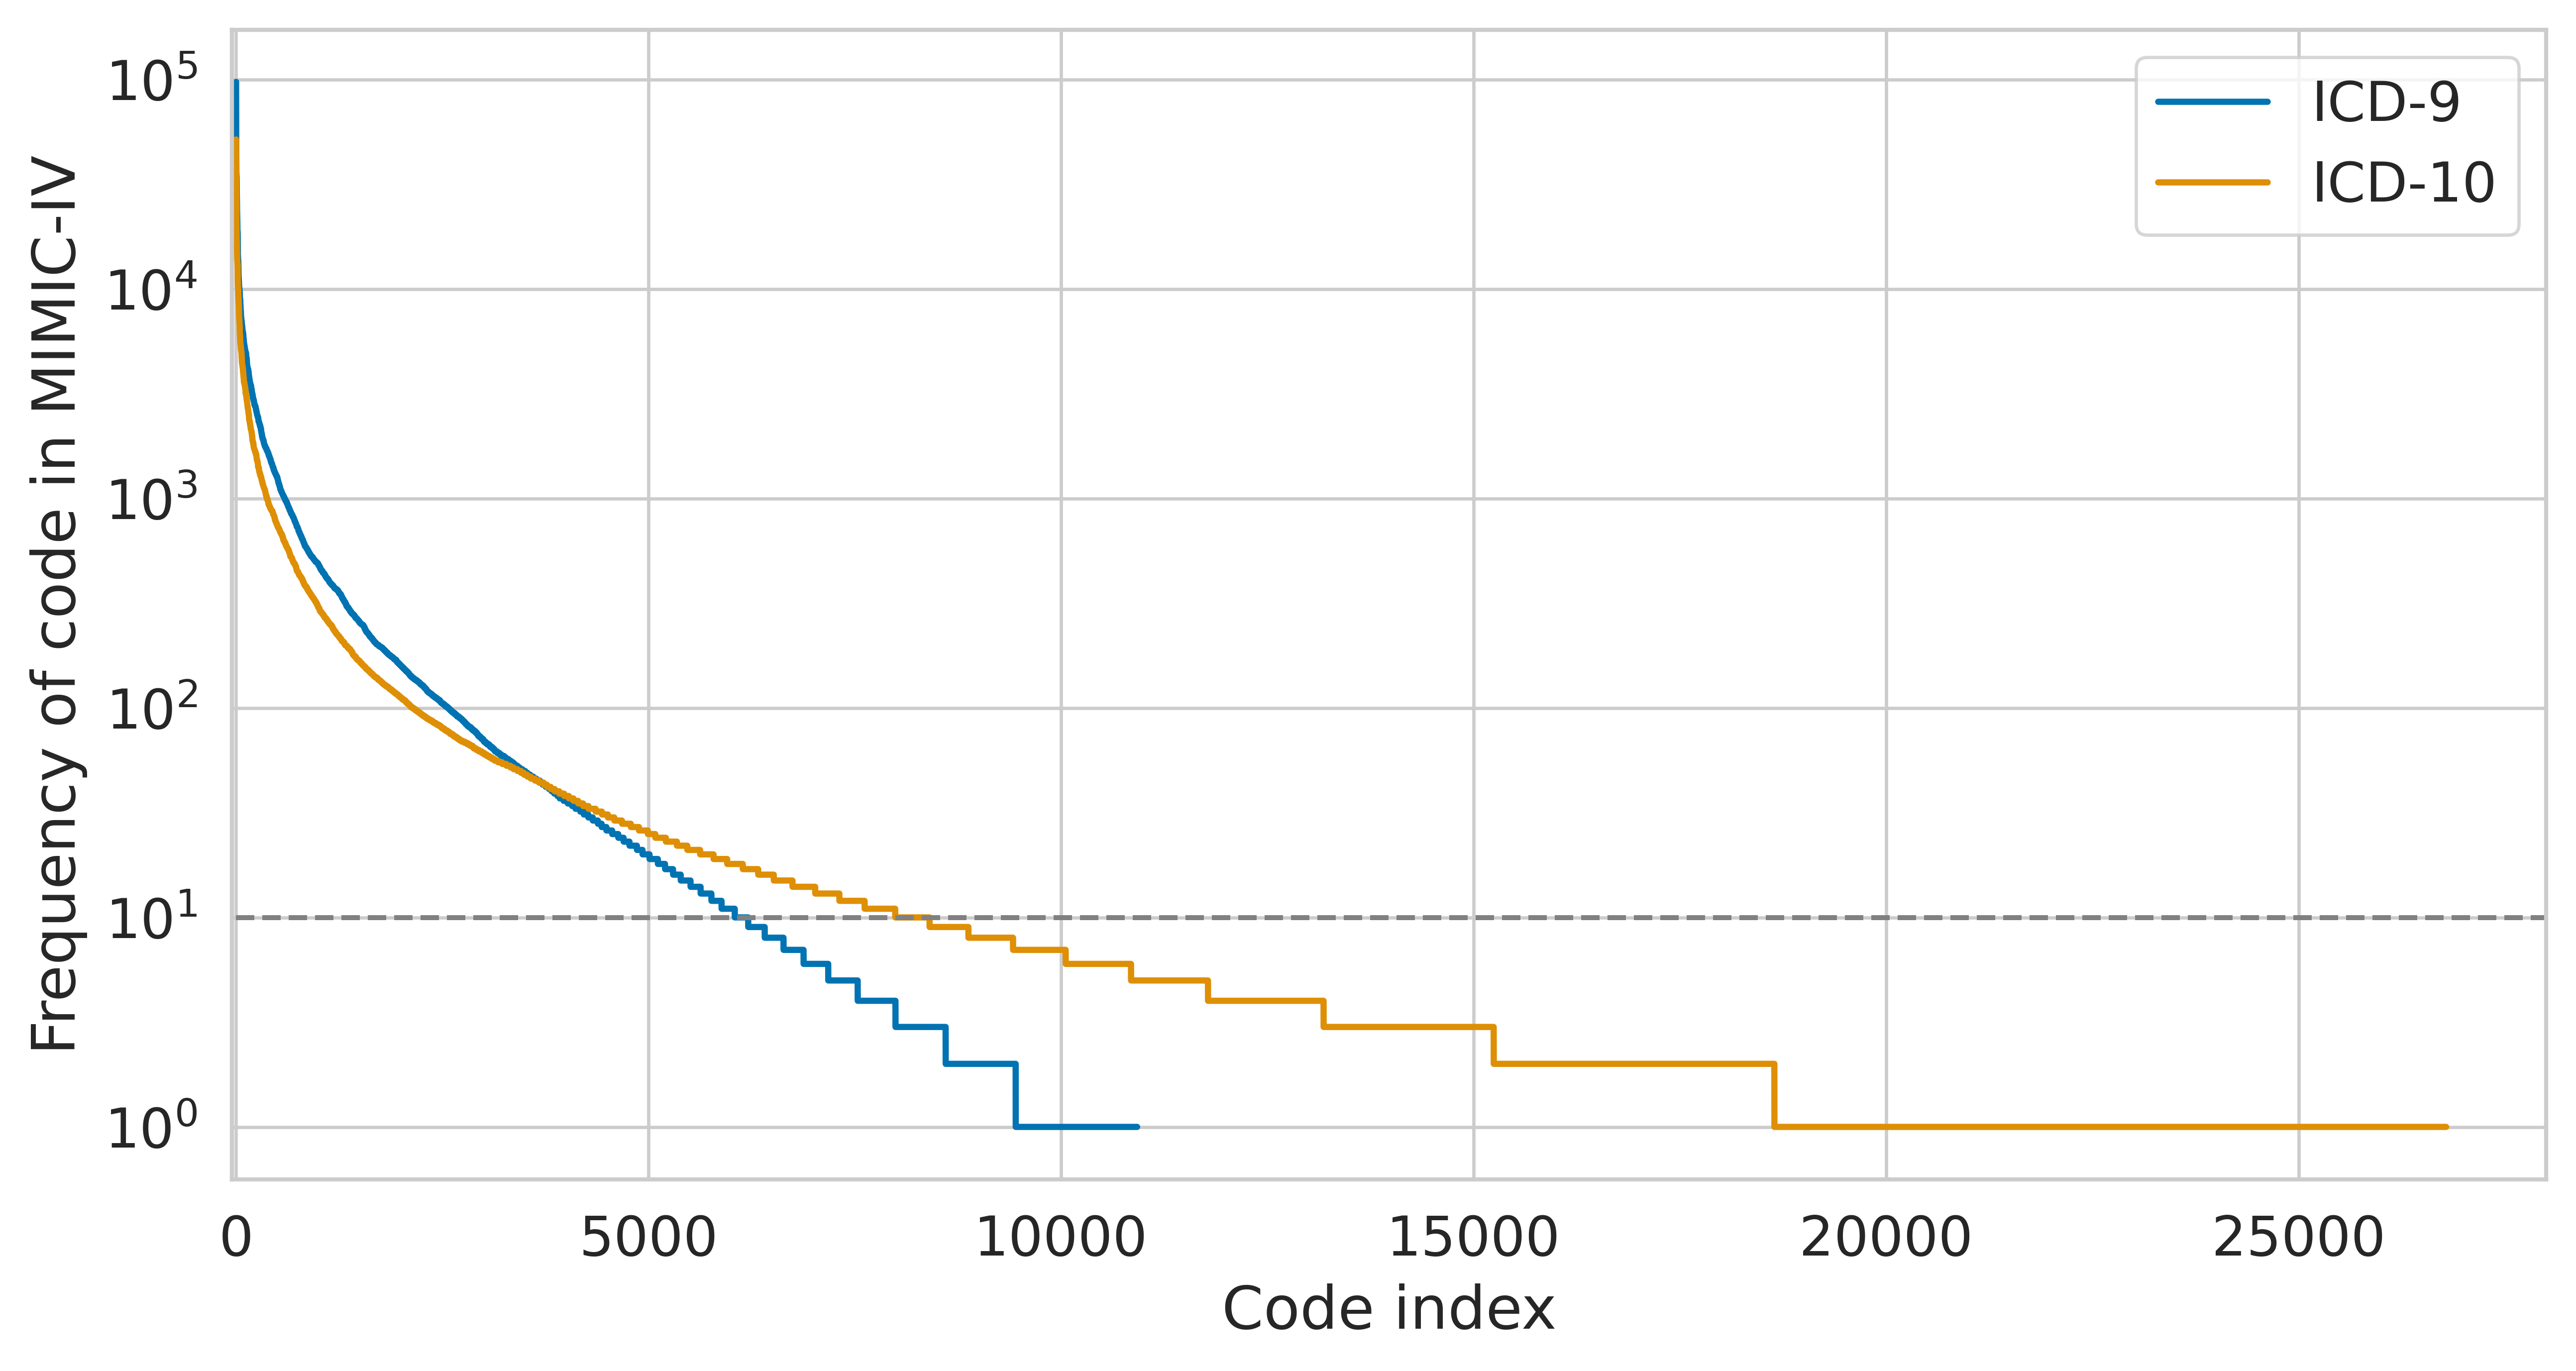
\includegraphics[width=0.9\textwidth]{paper_automated/mimiciv_code_freq.png}
    \caption[The frequency of ICD-9 and ICD-10 codes in MIMIC-IV before pre-processing.]{ The frequency of ICD-9 and ICD-10 codes in MIMIC-IV before pre-processing. As discussed in \cref{sec: splits}, we removed codes with fewer than ten instances (dashed line).}
    \label{fig:mimiciv_code_dist}
\end{figure}


\begin{sidewaystable}
    \centering
    \caption{Comparison of the previously defined MIMIC-III splits \textit{full} and \textit{50} \parencite{mullenbachExplainablePredictionMedical2018} and our proposed MIMIC-III \textit{clean} split along with similarly defined splits for MIMIC-IV \textit{ICD-9} and \textit{ICD-10} after pre-processing.}
    \label{tab:subsets}
    \resizebox*{\textwidth}{!}{%
    \begin{tabular}{lccccc}
        \toprule
        & \multicolumn{2}{c}{\textit{Previous work}} & \multicolumn{3}{c}{\textit{Our work}} \\
        \cmidrule(lr){2-3}\cmidrule(lr){4-6}
        & {MIMIC-III \textit{full}} & {MIMIC-III 50}  & {MIMIC-III \textit{clean}}  & {MIMIC-IV \textit{ICD-9}}  & {MIMIC-IV \textit{ICD-10}}\\
        \midrule
        Number of documents  & 52,723 & 11,368 &  52,712 & 209,326 & 122,279 \\
        Number of patients & 41,126 & 10,356 & 41,118 & 97,709 & 65,659 \\
        Number of unique codes  & 8,929 & 50  & 3,681 & 6,150 & 7,942\\
        Codes pr. instance: Median (IQR)    & 14 (10-20) & 5 (3-8) & 14 (10-20) & 12 (8-17) & 14 (9-20)\\
        Words pr. document: Median (IQR) & 1,375 (965-1,900) & 1,478 (1,065-1,992) & 1,311 (917-1,822) & 1,320 (997-1,715) & 1,492 (1,147-1,931)\\
        Documents: Train/val/test [\%] & 90.5/3.1/6.4 & 71.0/13.8/15.2 & 72.9/10.6/16.6  & 73.8/10.5/15.7& 72.9/10.9/16.2  \\
        Missing codes: Train/val/test [\%] & 2.7/66.4/54.3 & 0.0/0.0/0.0 & 0.0/0.1/0.0 & 0.0/0.5/0.2 & 0.0/0.5/0.1\\
        \bottomrule
    \end{tabular}%
    }
\end{sidewaystable}


\subsection{Model architectures}

Most recent state-of-the-art AMC models use an encoder-decoder architecture. The encoder takes a sequence of tokens $T \in \mathbb{Z}^{n}$ as input and outputs a sequence of hidden representations $H \in \mathbb{R}^{d_h \times n}$, where $n$ is the number of tokens in a sequence, and $d_h$ is the hidden dimension. The decoder takes $H$ as input and outputs the code probability distributions. For the task of ranking, codes are sorted by decreasing probability. For classification, code probabilities larger than a set decision boundary are predicted. 

\paragraph{Encoders:}
The encoder usually consists of pre"=trained non-contextualized word embeddings (e.g., Word2Vec) and a neural network for encoding context. More recently, pre"=trained masked language models (e.g., BERT) have gained popularity~\parencite{tengReviewDeepNeural2022}. The MIMIC-III training set or PubMed articles are commonly used for pre"=training.

\paragraph{Decoders:}
The most common decoder architectures can be grouped into three primary types. 
The simplest decoder is a pooling layer (e.g., max pooling) followed by a feed-forward neural network. More recently, label-wise attention (LA) \parencite{mullenbachExplainablePredictionMedical2018} has replaced pooling \parencite{vuLabelAttentionModel2020, liuEffectiveConvolutionalAttention2021, huangPLMICDAutomaticICD2022, liICDCodingClinical2020}. LA transforms a sequence of hidden representations $H$ into label-specific representations $V \in \mathbb{R}^{d_h \times L}$, where $L$ is the number of unique medical codes in the dataset.
It is computed as
\begin{equation}
    A = \text{softmax}(WH) \, , \quad
    V = HA^{\top} \enspace ,
\end{equation}
where the softmax normalizes each column of $WH$, $W \in \mathbb{R}^{L \times d_h}$ is an embedding matrix that learns label-specific queries, and $A \in \mathbb{R}^{L \times n}$ is the attention matrix. 
Then, $V$ is used to compute class-wise probabilities via a feedforward neural network. 
As LA was first used in the \textit{convolutional attention for multi-label classification} (CAML) model~\parencite{mullenbachExplainablePredictionMedical2018}, we refer to this method as \lacaml.

An updated label-wise attention module was introduced in the \textit{label attention model} (LAAT) \parencite{vuLabelAttentionModel2020}. We refer to this attention module as \lalaat. In \lalaat, the label-specific attention is computed similarly to  \lacaml~ as $A = \text{softmax}(UZ)$, where $U \in \mathbb{R}^{L \times d_p}$ is a learnable embedding matrix, but with 
$Z = \text{tanh}(PH)$ 
where $P \in \mathbb{R}^{d_p \times d_h}$ is a learnable matrix, $Z \in \mathbb{R}^{d_p \times n}$ and $d_p$ is a hyperparameter.


\subsection{Training and evaluation methods}\label{sec: training and evaluation methods}

\textcite{mullenbachExplainablePredictionMedical2018} released code for pre-processing the discharge summaries, generating the train-test split, and evaluating model performance on MIMIC-III which many subsequent papers have used \parencite{vuLabelAttentionModel2020, huangPLMICDAutomaticICD2022, liICDCodingClinical2020, baoMedicalCodePrediction2021, yuanCodeSynonymsMatter2022, kimReadAttendCode2021}.
Pre-processing consisted of lower-casing all text and removing words that only contain out-of-alphabet characters. Predicting procedures and diagnosis codes were treated as a single task.
The dataset was split into training, validation, and test sets using random sampling, ensuring that no patient occurred in both the training and test set. The (non-stratified) random sampling lead to 54\% of the ICD codes in MIMIC-III \textit{full} not being sampled in the test set. This complicates the interpretation of results since these codes only contribute true negatives or false positives. 
Models are evaluated using the micro and macro average of the area under the curve of the receiver operating characteristics (AUC-ROC), F1-score, and precision@k. 

While most papers use the pre-processing, train-test split, and evaluation metrics described above, they differ in several aspects of training. This may lead to performance differences unrelated to modeling choices which are undesirable when seeking to compare models. 
For instance, due to varying memory constraints of different models, documents are usually truncated to some maximum length. In the literature, this maximum varies from 2,500 to 4,000 words \parencite{mullenbachExplainablePredictionMedical2018, vuLabelAttentionModel2020, huangPLMICDAutomaticICD2022}.
Furthermore, not all papers tune the prediction decision boundary but simply set it to 0.5,
 hyperparameter search ranges and sampling methods  vary between works, and learning rate schedulers are only used in LAAT and PLM-ICD\parencite{mullenbachExplainablePredictionMedical2018, liICDCodingClinical2020}. In LAAT, the learning rate was decreased by 90\% when the F1-score had not increased for five epochs. PLM-ICD used a schedule with linear warm up followed by linear decay. 

All models except for PLM-ICD use Word2Vec embeddings pre"=trained on the MIMIC-III training set. PLM-ICD uses a BERT encoder pre"=trained on PubMed to encode the text in chunks of 128 tokens, and these contextualized embeddings are fed to a \lalaat~ layer. 

Finally, all models compute independent code probabilities using sigmoid activation functions and optimize the binary cross entropy loss function during training.
\cref{tab:model_facts} presents the selected models.


\section{Methods}

\begin{table}
    \centering
    \caption{An overview of the compared models.}
    \label{tab:model_facts}
    \begin{tabular}{llllr}
        \toprule
        Model   & Encoder & Decoder  & Param \\
        \midrule
        Bi-GRU \parencite{mullenbachExplainablePredictionMedical2018}   &  Word2Vec, Bi-GRU & Max-pool  &  9.9M\\
        CNN \parencite{mullenbachExplainablePredictionMedical2018}   & Word2Vec, CNN & Max-pool &  10.3M\\
        CAML \parencite{mullenbachExplainablePredictionMedical2018}   & Word2Vec, CNN  & \lacaml &  6.1M\\
        MultiResCNN \parencite{liICDCodingClinical2020} &  Word2Vec, ResNet & \lacaml &  11.9M\\
        LAAT \parencite{vuLabelAttentionModel2020} & Word2Vec, Bi-LSTM  & \lalaat  &  21.9M\\
        PLM-ICD \parencite{huangPLMICDAutomaticICD2022} &  BERT & \lalaat &  138.8M\\
        \bottomrule
    \end{tabular}
\end{table}

\subsection{Selection criteria}\label{sec: inclusion and exclusion criteria}

In this study, we included both models trained from scratch and models with components pre"=trained on external corpora. 
We excluded models that use multi-modal inputs, such as medical code descriptions \parencite{kimReadAttendCode2021, mullenbachExplainablePredictionMedical2018, vuLabelAttentionModel2020, caoHyperCoreHyperbolicCograph2020, baoMedicalCodePrediction2021}, code synonyms \parencite{yuanCodeSynonymsMatter2022}, code hierarchies \parencite{caoHyperCoreHyperbolicCograph2020, xieEHRCodingMultiscale2019}, or associated Wikipedia articles \parencite{baiImprovingMedicalCode2019}, because they introduced additional complexity without providing evidence for significant performance improvements \parencite{mullenbachExplainablePredictionMedical2018, vuLabelAttentionModel2020, tengReviewDeepNeural2022}. We excluded works without publically available source code as the experiment descriptions often lacked important implementation details.

\subsection{Evaluation metrics}
\label{sec:metrics}
Similar to previous work, we evaluated models using AUC-ROC, F1-score, and precision@$k$. Additionally, we introduced exact match ratio (EMR), R-precision, and mean average precision (MAP). The EMR is the percentage of instances where all codes were predicted correctly. This allowed us to measure how many documents were predicted perfectly, which is important for \textit{fully automated} medical coding.
Where precision@$k$ is computed based on the top-$k$ codes (i.e., $k$ is fixed), R-precision considers a number of codes equal to the true number of relevant codes. Thus, R-precision is useful when the number of relevant codes varies considerably between documents, which is the case for the MIMIC datasets. Finally, in contrast to all other metrics, MAP considers the exact rank of all relevant codes in a document.


\begin{sidewaystable}
    \centering
    \caption[Hyperparameters, maximum document lengths, and decision boundary tuning strategies used in the original works compared to improved settings.]{ Hyperparameters, maximum document lengths, and decision boundary tuning strategies used in the original works compared to the optimal settings found in this paper (marked with *). LR is the learning rate scheduler. ``Length" is the maximum number of words a document can contain before being truncated. $\dagger$ applies to models using word-piece tokenization. These models were filtered on the number of sub-words instead of full words. ``DB tune" is whether the optimal decision boundary was found using the validation set. If a paper did not tune the decision boundary, it was set to 0.5.}
    \label{tab:hyperparameters}
    \resizebox*{\textwidth}{!}{%
    \begin{tabular}{lccccccccc}
        \toprule
        & \multicolumn{7}{c}{Hyperparameters} & & \\
        \cmidrule(lr){2-8}
        Model & Batch Size & Weight Decay & Learning Rate & Dropout & LR Scheduler & Optimizer & Epochs & Length & DB tune \\
        \midrule
        Bi-GRU  & 16 &  0.0 & 0.003 &  0.2   & no  & Adam &  100 & 2500 & no\\
        Bi-GRU$^*$  & 8 &  0.0001 & 0.001 &  0   & yes  & AdamW &  20 & 4000 & yes\\
        \hline
        CNN  & 16 &  0.0 & 0.003  &  0.2 & no  & Adam &  100 & 2500 & no\\
        CNN$^*$    & 8 &  0.00001 & 0.001  &  0 & yes  & AdamW &  20 & 4000 & yes \\
        \hline
        CAML  & 16 &  0.0 & 0.0001  &  0.2  & no  & Adam  &  200 & 2500 & no\\
        CAML$^*$    & 8 &  0.001 & 0.005  &  0.2  & yes  & AdamW  &  20 & 4000 & yes\\
        \hline
        MultiResCNN & 16 &  0.0 & 0.0001  &  0.2  & no  & Adam &  200 & 2500 & no\\
        MultiResCNN$^*$  & 16 &  0.0001 & 0.0005  &  0.2  & yes  & AdamW &  20 & 4000 & yes\\
        \hline
        LAAT   & 8 &  0.0 & 0.0001  &  0.3  & yes  & AdamW &  50 & 4000 & no\\
        LAAT$^*$    & 8 &  0.001 & 0.001  &  0.2  & yes  & AdamW &  20 & 4000 & yes\\
        \hline
        PLM-ICD  & 8 &  0.0 & 0.00005  &  0.2  & yes  & AdamW &  20 & 3072$^\dagger$ & yes \\
        PLM-ICD$^*$   & 16 &  0.0 & 0.00005  &  0.2  & yes  & AdamW &  20 & 4000 & yes \\
        \bottomrule
    \end{tabular}%
    }
\end{sidewaystable}


Previous works calculated the macro F1-score as the harmonic mean of the macro precision and macro recall \parencite{mullenbachExplainablePredictionMedical2018, liICDCodingClinical2020, vuLabelAttentionModel2020, huangPLMICDAutomaticICD2022}. \textcite{opitzMacroF1Macro2021} analyze macro F1 formulas common in multi-class and multi-label classification. They demonstrate that the above formulation is suboptimal, as it rewards heavily biased classifiers in unbalanced datasets. Therefore, as recommended by the authors, we calculated the macro F1-score as the arithmetic mean of the F1-score for each class.
As seen in \cref{tab:subsets}, 54\% of codes in MIMIC-III \textit{full} are missing in the test set. Previous works set the F1-score of all the missing codes in the test set to 0, resulting in a misleadingly low macro F1-score. Because 54\% of the codes are missing, the maximum possible macro F1-score is 46\%. 
We ignored all codes not in the test set for our reproduction, essentially trading bias for variance. 
For our revised comparison, we resolved the issue by instead sampling new splits that reduce missing codes to a negligible fraction (see \cref{sec: splits}) and ignoring the few that were still missing.


\subsection{Definition of splits}
\label{sec: splits}

% \cref{tab:subsets}

We define three new splits: MIMIC-III \textit{clean}, MIMIC-IV \textit{ICD-9}, and \textit{ICD-10}.
As described in \cref{sec:metrics}, 54\% of the codes in MIMIC-III \textit{full} are absent from the test set, which introduces significant bias in the model evaluation metrics. Therefore, we created a new MIMIC-III split to ensure that most codes are present in both the training and test set. 
Specifically, we removed codes with fewer than ten occurrences, doubled the test set size, and sampled the documents using multi-label stratified sampling \parencite{sechidisStratificationMultilabelData2011}. 
We ensured that no patient occurred in both the training and test set, preprocessed the text, and considered procedures and diagnosis codes as a single task as done by \textcite{mullenbachExplainablePredictionMedical2018}.
We based our new split on the v1.4 version of the dataset and refer to it as MIMIC-III \textit{clean}.
Using the same method, we created two splits for MIMIC-IV v2.2: one containing all documents labeled with ICD-9 codes and one with ICD-10 codes.


\subsection{Reproducibility experiments}

We ran reproducibility experiments with all models to evaluate whether the results in the original works could be reproduced and to validate our reimplementations. We ran these experiments on MIMIC-III \textit{full}, and \textit{50} as in the original works \parencite{mullenbachExplainablePredictionMedical2018,liICDCodingClinical2020,vuLabelAttentionModel2020,huangPLMICDAutomaticICD2022}. We used the hyperparameters reported in each paper (see \cref{tab:hyperparameters}) and report both the original and the revised macro F1-scores discussed in \cref{sec:metrics}.

\subsection{Revised comparison}
To address the issues associated with comparing results reported by previous works described in \cref{sec: training and evaluation methods,sec:metrics}, we perform a revised model comparison. We run experiments on the new MIMIC-III \textit{clean}, MIMIC-IV \textit{ICD-9}, and \textit{ICD-10}.
All models were trained for 20 epochs using a learning rate schedule with linear warm up for the first 2K updates followed by linear decay \parencite{huangPLMICDAutomaticICD2022}. We found this schedule to speed up the training convergence of all the models.
Whereas original works use Adam or AdamW, we used AdamW for all experiments as it corrects the weight decay implementation of Adam \parencite{kingmaAdamMethodStochastic2017, loshchilovDecoupledWeightDecay2022}. For each model, we tuned the decision boundary to maximize the micro F1-score on the validation set. We used randomized sampling to find optimal settings for dropout, weight decay, learning rate, and batch size. The hyperparameter search was performed on MIMIC-III \textit{clean}, and the MIMIC-IV splits. We found that the best setting for each model generalized across datasets. Using this setting, we ran each model ten times with different seeds on each dataset. All documents were truncated to a maximum of 4000 words. The hyperparameters, maximum document lengths, and decision boundary tuning strategy are summarized in \cref{tab:hyperparameters}. 

We performed an ablation study to analyze which changes had the largest impact on performance. 
Specifically, we evaluated the effect of truncation, hyperparameter search, and decision boundary tuning. We modified one of these at a time: We ran one experiment where documents were truncated to a maximum length of 2,500 words, a second experiment where the models were trained with the hyperparameters, number of epochs, and learning rate schedule used in the original works, and a third experiment where the decision boundary was set to 0.5 instead of tuned.

\subsection{Error analysis}
To validate and falsify the commonly cited challenges of AMC, which include a lack of training data, long documents, and rare codes, we performed an error analysis. In addition to analyzing rare codes, we contribute an in-depth code analysis aiming to identify the attributes that make certain codes challenging to predict.


\paragraph{Amount of training data:}
Multiple studies attribute poor performance to data sparsity of MIMIC-III, which contains only fifty thousand examples \parencite{kavuluruEmpiricalEvaluationSupervised2015,tengExplainablePredictionMedical2020,yanMedicalCodingClassification2010,yangKnowledgeInjectedPrompt2022}. MIMIC-IV \textit{ICD-9} contains four times as many examples, which allows analyzing the effect of training set size. We train each model on 25k, 50k, 75k, 100k, and 125k examples and report micro and macro F1 on the fixed test set. The training subsets were sampled from the training set using multi-label stratified sampling to ensure the same code distributions \parencite{sechidisStratificationMultilabelData2011}.

\paragraph{Document length:}
We analyzed whether model performance correlates with document length on MIMIC-IV \textit{ICD-9}. Specifically, we calculated the Pearson and Spearman correlation between the number of words in the documents and the micro F1-score for all models. For each model, we used the best seed from the revised comparison.

\paragraph{Code analysis:}
To analyze the performance impact of rare codes, we first calculated the Pearson and Spearman correlation between model performance on each code and the corresponding code frequency in the training data. We calculated these correlations for all splits. To identify attributes of challenging codes, we analyzed model performance on the chapter level of the ICD-10 classification system. Using high-level chapters instead of codes allows us to group examples into categories, which we use as a starting point for further analysis. We limit the scope of the analysis to diagnosis codes. We focused on ICD-10 because it is the classification system currently in use at most hospitals. 


\begin{sidewaystable}
    \centering
    \caption[Reproduced test set results compared with those from the original works.]{ Reproduced test set results compared with those from the original works. Our reproduced results are indicated with *. The results were reproduced on MIMIC-III v1.4 with the preprocessing pipeline and splits of \textcite{mullenbachExplainablePredictionMedical2018}. Each model was reproduced using the hyperparameters presented in the respective paper. We use both macro F1 formulas: Macro$^\dagger$ refers to the method used in the original work, while Macro refers to the corrected version used in this paper.}
    \label{tab:reproduced_results}
    \resizebox*{\textwidth}{!}{%
    \begin{tabular}{l  cc  ccc  cc  cc  ccc  c}
        \toprule
        & \multicolumn{7}{c}{MIMIC-III \textit{full}} & \multicolumn{6}{c}{MIMIC-III \textit{50}} \\
        \cmidrule(lr){2-8}\cmidrule(lr){9-14}
        & \multicolumn{2}{c}{AUC-ROC} & \multicolumn{3}{c}{F1} & \multicolumn{2}{c}{Precision@$k$}  & \multicolumn{2}{c}{AUC-ROC} & \multicolumn{3}{c}{F1} & Precision@$k$  \\
        & Micro & Macro & Micro & Macro$^\dagger$ & Macro & 8 & 15 & Micro & Macro & Micro & Macro$^\dagger$ & Macro & 5 \\
        \midrule
        CNN &  96.9 & 80.6 &  41.9& 4.2 & -& 58.1 &  48.8  & 90.7 & 87.6 & 62.5 & 57.6 & - & 62.0  \\
        CNN$^*$ & 97.3 & 83.1 & 41.5 & 3.4 & 6.7 & 61.9 & 47.2 & 91.9 & 89.2 & 64.9 & 58.8 & 58.0 &  62.6 \\
        \hline
        Bi-GRU & 97.1 & 82.2 & 41.7 & 3.8 & - & 58.5 & 44.5  &  89.2 & 82.8 & 54.9 &  48.4 & - &  59.1  \\
        Bi-GRU$^*$  & 98.0 & 87.1 & 42.6 & 3.6 & 7.0 & 65.0 & 49.8 & 89.3 & 85.2 & 56.1 & 46.2 & 43.1 & 57.9  \\
        \hline
        CAML  &  98.6 &  89.5 &  53.9 & 8.8 & - &  70.9 &  56.1  & 90.9 & 87.5 &  61.4 &  53.2 & - &   60.9  \\
        CAML$^*$ & 98.4 & 88.4 & 49.5 & 5.6 & 11.3 & 69.9 & 54.9 & 91.1 & 87.5 & 60.6 & 52.4 & 51.0 & 61.1  \\
        \hline
        MultiResCNN  &  98.6 &  91.0 & 55.2 & 8.6 & - & 73.4 & 58.4  &  93.8 &  89.9 &  67.0 &  60.6 & - &  64.1 \\
        MultiResCNN$^*$  & 98.6 & 90.8 & 56.5 & 9.2 & 18.5 & 73.4 & 58.4 & 92.4 & 89.7 & 67.3 & 62.2 & 61.1 & 63.4  \\
        \hline
        LAAT  &  98.8 &  91.9 &  57.5 & 9.9 & - &  74.5 &  59.1  &  94.6 &  92.5 &  71.5 &  66.6 & - &  67.5 \\
        LAAT$^*$ & 98.6 & 89.5 & 56.1 & 8.2 & 16.2 & 73.9 & 58.7 & 92.8 & 90.5 & 66.8 & 60.8 & 59.2 & 64.0  \\
        \hline
        PLM-ICD  &  98.9 & 92.6 &  59.8 & 10.4 & - &  77.1 &  61.3  & - & - & - & - & - & -  \\
        PLM-ICD$^*$ & 98.8 & 92.3 & 58.9 & 11.1 & 22.8 & 75.7 & 60.5 & 93.8 & 91.7 & 70.5 & 66.3 & 65.4 & 65.7 \\
        \bottomrule
    \end{tabular}%
    }
\end{sidewaystable}

\section{Results}
\subsection{Reproduced results}


In \cref{tab:reproduced_results}, we report the reproduced results on MIMIC-III \textit{full} and \textit{50} using hyperparameters as reported in the original papers. We list the original and corrected macro F1-score described in \cref{sec:metrics}. In most cases, our corrections doubled the macro F1-scores on MIMIC-III \textit{full}. The differences were smaller on MIMIC-III \textit{50} because all included codes are in the test set.


\subsection{Revised comparison}

\begin{sidewaystable}
    \centering
    \caption[Results on the MIMIC-III \textit{clean}, MIMIC-IV \textit{ICD-9} and MIMIC-IV  \textit{ICD-10} test sets presented as percentages.]{ Results on the MIMIC-III \textit{clean}, MIMIC-IV \textit{ICD-9} and MIMIC-IV  \textit{ICD-10} test sets presented as percentages. Micro F1-scores rank the table in ascending order. Each model was trained ten times with different seeds. We performed a McNemar's test with Bonferroni correction and found that all the models are significantly different ($p < 0.001$).}
    \label{tab:fair_results}
    \resizebox*{\textwidth}{!}{%
    \begin{tabular}{llccccccccc}
        \toprule
        & & \multicolumn{5}{c}{Classification} & \multicolumn{4}{c}{Ranking} \\ 
        \cmidrule(lr){3-7}\cmidrule(lr){8-11}
         & & \multicolumn{2}{c}{AUC-ROC} & \multicolumn{2}{c}{F1} & EMR & \multicolumn{2}{c}{Precision@k} & R-precision & MAP \\
         & & Micro & Macro & Micro & Macro &  & 8 & 15 &  &  \\
        \midrule
        \multirow{6}{*}{\shortstack[c]{MIMIC-III \\ clean}} & CNN & 97.1$\pm$0.0 & 88.1$\pm$0.2 & 48.0$\pm$0.3 & 9.9$\pm$0.4 & 0.1$\pm$0.0 & 61.6$\pm$0.2 & 46.6$\pm$0.1 & 49.1$\pm$0.2 & 50.6$\pm$0.2 \\
        & Bi-GRU  & 97.8$\pm$0.1 & 91.1$\pm$0.2 & 49.7$\pm$0.4 & 12.2$\pm$0.2 & 0.1$\pm$0.0 & 62.8$\pm$0.4 & 47.6$\pm$0.4 & 50.1$\pm$0.4 & 52.1$\pm$0.4 \\
        & CAML & 98.2$\pm$0.0 & 91.4$\pm$0.2 & 55.4$\pm$0.1 & 20.4$\pm$0.3 & 0.1$\pm$0.0 & 67.7$\pm$0.2 & 52.8$\pm$0.1 & 55.8$\pm$0.1 & 58.9$\pm$0.2 \\
        & MultiResCNN & 98.5$\pm$0.0 & 93.1$\pm$0.3 & 56.4$\pm$0.2 & 22.9$\pm$0.6 & 0.1$\pm$0.0 & 68.5$\pm$0.2 & 53.5$\pm$0.1 & 56.7$\pm$0.2 & 59.9$\pm$0.3 \\
        & LAAT & 98.6$\pm$0.1 & 94.0$\pm$0.3 & 57.8$\pm$0.2 & 22.6$\pm$0.6 & 0.2$\pm$0.1 & 70.1$\pm$0.2 & 54.8$\pm$0.2 & 58.0$\pm$0.2 & 61.7$\pm$0.3 \\
        & PLM-ICD & \bfseries 98.9$\pm$0.0 & \bfseries 95.9$\pm$0.1 & \bfseries 59.6$\pm$0.2 & \bfseries 26.6$\pm$0.8 & \bfseries 0.4$\pm$0.0 & \bfseries 72.1$\pm$0.2 & \bfseries 56.5$\pm$0.1 & \bfseries 60.1$\pm$0.1 & \bfseries 64.6$\pm$0.2 \\
        \hline
        \multirow{6}{*}{\shortstack[c]{MIMIC-IV \\ ICD-9}} & CNN  & 98.1$\pm$0.1 & 89.4$\pm$0.5 & 52.4$\pm$0.1 & 12.6$\pm$0.4 & 0.6$\pm$0.0 & 61.3$\pm$0.1 & 45.6$\pm$0.0 & 52.9$\pm$0.1 & 55.2$\pm$0.1 \\
        & Bi-GRU  & 98.8$\pm$0.0 & 93.8$\pm$0.1 & 55.5$\pm$0.1 & 16.6$\pm$0.2 & 0.7$\pm$0.0 & 64.1$\pm$0.1 & 47.8$\pm$0.1 & 55.8$\pm$0.1 & 58.9$\pm$0.1 \\
        & CAML & 98.8$\pm$0.0 & 90.7$\pm$0.3 & 58.6$\pm$0.1 & 19.3$\pm$0.1 & 0.6$\pm$0.0 & 66.3$\pm$0.1 & 50.3$\pm$0.0 & 58.5$\pm$0.1 & 62.4$\pm$0.1 \\
        & MultiResCNN  & 99.2$\pm$0.0 & 95.1$\pm$0.1 & 60.4$\pm$0.0 & 27.7$\pm$0.3 & 0.8$\pm$0.0 & 67.6$\pm$0.0 & 51.8$\pm$0.0 & 60.4$\pm$0.0 & 64.7$\pm$0.1 \\
        & LAAT  & 99.3$\pm$0.0 & 96.0$\pm$0.3 & 61.7$\pm$0.1 & 26.4$\pm$0.9 & 0.9$\pm$0.0 & 68.9$\pm$0.1 & 52.7$\pm$0.1 & 61.7$\pm$0.2 & 66.3$\pm$0.2 \\
        & PLM-ICD  & \bfseries 99.4$\pm$0.0 & \bfseries 97.2$\pm$0.2 & \bfseries 62.6$\pm$0.3 & \bfseries 29.8$\pm$1.0 & \bfseries 1.0$\pm$0.1 & \bfseries 70.0$\pm$0.2 & \bfseries 53.5$\pm$0.2 & \bfseries 62.7$\pm$0.3 & \bfseries 68.0$\pm$0.3 \\
        \hline
        \multirow{6}{*}{\shortstack[c]{MIMIC-IV \\ ICD-10}} & CNN & 97.5$\pm$0.1 & 87.9$\pm$0.4 & 47.2$\pm$0.6 & 8.0$\pm$0.4 & 0.3$\pm$0.0 & 60.3$\pm$0.1 & 45.7$\pm$0.1 & 47.3$\pm$0.2 & 48.2$\pm$0.2 \\
        & Bi-GRU  & 98.3$\pm$0.0 & 92.4$\pm$0.2 & 50.1$\pm$0.2 & 10.6$\pm$0.4 & 0.3$\pm$0.0 & 62.6$\pm$0.2 & 47.7$\pm$0.2 & 49.6$\pm$0.1 & 51.1$\pm$0.2 \\
        & CAML  & 98.5$\pm$0.0 & 91.1$\pm$0.1 & 55.4$\pm$0.2 & 16.0$\pm$0.3 & 0.3$\pm$0.0 & 66.8$\pm$0.2 & 52.2$\pm$0.1 & 54.5$\pm$0.2 & 57.4$\pm$0.2 \\
        & MultiResCNN  & 99.0$\pm$0.0 & 94.5$\pm$0.2 & 56.9$\pm$0.1 & \bfseries 21.1$\pm$0.2 & \bfseries 0.4$\pm$0.0 & 67.8$\pm$0.1 & 53.5$\pm$0.1 & 56.1$\pm$0.1 & 59.3$\pm$0.2 \\
        & LAAT  & 99.0$\pm$0.1 & 95.4$\pm$0.3 & 57.9$\pm$0.1 & 20.3$\pm$0.4 & \bfseries 0.4$\pm$0.0 & 68.9$\pm$0.1 & 54.3$\pm$0.1 & 57.2$\pm$0.1 & 60.6$\pm$0.2 \\
        & PLM-ICD   & \bfseries 99.2$\pm$0.0 & \bfseries 96.6$\pm$0.2 & \bfseries 58.5$\pm$0.7 & \bfseries 21.1$\pm$2.3 & \bfseries 0.4$\pm$0.0 & \bfseries 69.9$\pm$0.6 & \bfseries 55.0$\pm$0.6 & \bfseries 57.9$\pm$0.8 & \bfseries 61.9$\pm$0.9 \\
        
        \bottomrule
    \end{tabular}%
    }
\end{sidewaystable}

The results of our revised comparison on MIMIC-III \textit{clean}, MIMIC-IV \textit{ICD-9}, and \textit{ICD-10} are shown in \cref{tab:fair_results}. Contrary to the originally reported results, Bi-GRU performs better than CNN in all metrics. Otherwise, the model performance ranking is unchanged from the original works. PLM-ICD outperformed the other models on all metrics and all datasets. The models previously reported as least performant improved the most. 

The ablation study results are shown in \cref{tab:ablation_study} for MIMIC-III \textit{clean}. Truncating the documents to 2,500 words instead of 4,000 had little impact on the performance. Using the hyperparameters from the original works degraded the performance substantially for CAML, Bi-GRU, and CNN but had a smaller effect on the other models. Not tuning the decision boundary had the largest negative effect on all models except MultiResCNN. In \cref{fig:threshold_tuning}, we plot the relationship between the decision boundary and F1-scores. LAAT and MultiResCNN perform similarly when using a decision boundary of 0.5. However, when tuning the decision boundary, LAAT outperforms MultiResCNN considerably.
Similar results were obtained on the other datasets. 

\begin{sidewaystable}
    \centering
    \caption[Ablation study on MIMIC-III \textit{clean}.]{ Ablation study on MIMIC-III \textit{clean}. The numbers are the micro/macro F1-scores on the test set.}
    \label{tab:ablation_study}
    \resizebox*{\textwidth}{!}{%
    \begin{tabular}{lcccccc}
        \toprule
         & PLM-ICD & LAAT & MultiResCNN & CAML & Bi-GRU & CNN \\
        \midrule
        Our result & 59.6/26.6 & 57.8/22.6 & 56.4/22.9 & 55.4/20.4 & 49.7/12.2 & 48.0/9.9 \\
        \hline
        Input length truncated at 2500 words & 59.4/26.2 & 57.6/22.3 & 56.0/23.2 & 54.8/19.7 & 49.4/12.0 & 47.9/9.8 \\
        No decision boundary tuning & 58.7/23.0 & 56.2/19.0 & 56.2/22.6 & 53.3/17.1 & 45.3/8.1 & 43.8/7.0 \\
        Original hyperparameters & 59.6/27.0 & 57.5/21.6 & 56.4/20.0 & 52.8/17.3 & 48.1/11.2 & 46.9/10.2 \\
        \bottomrule
        \end{tabular}%
    }
\end{sidewaystable}


\begin{figure}
    \centering
    \begin{subfigure}[b]{0.9\textwidth}
        \centering
        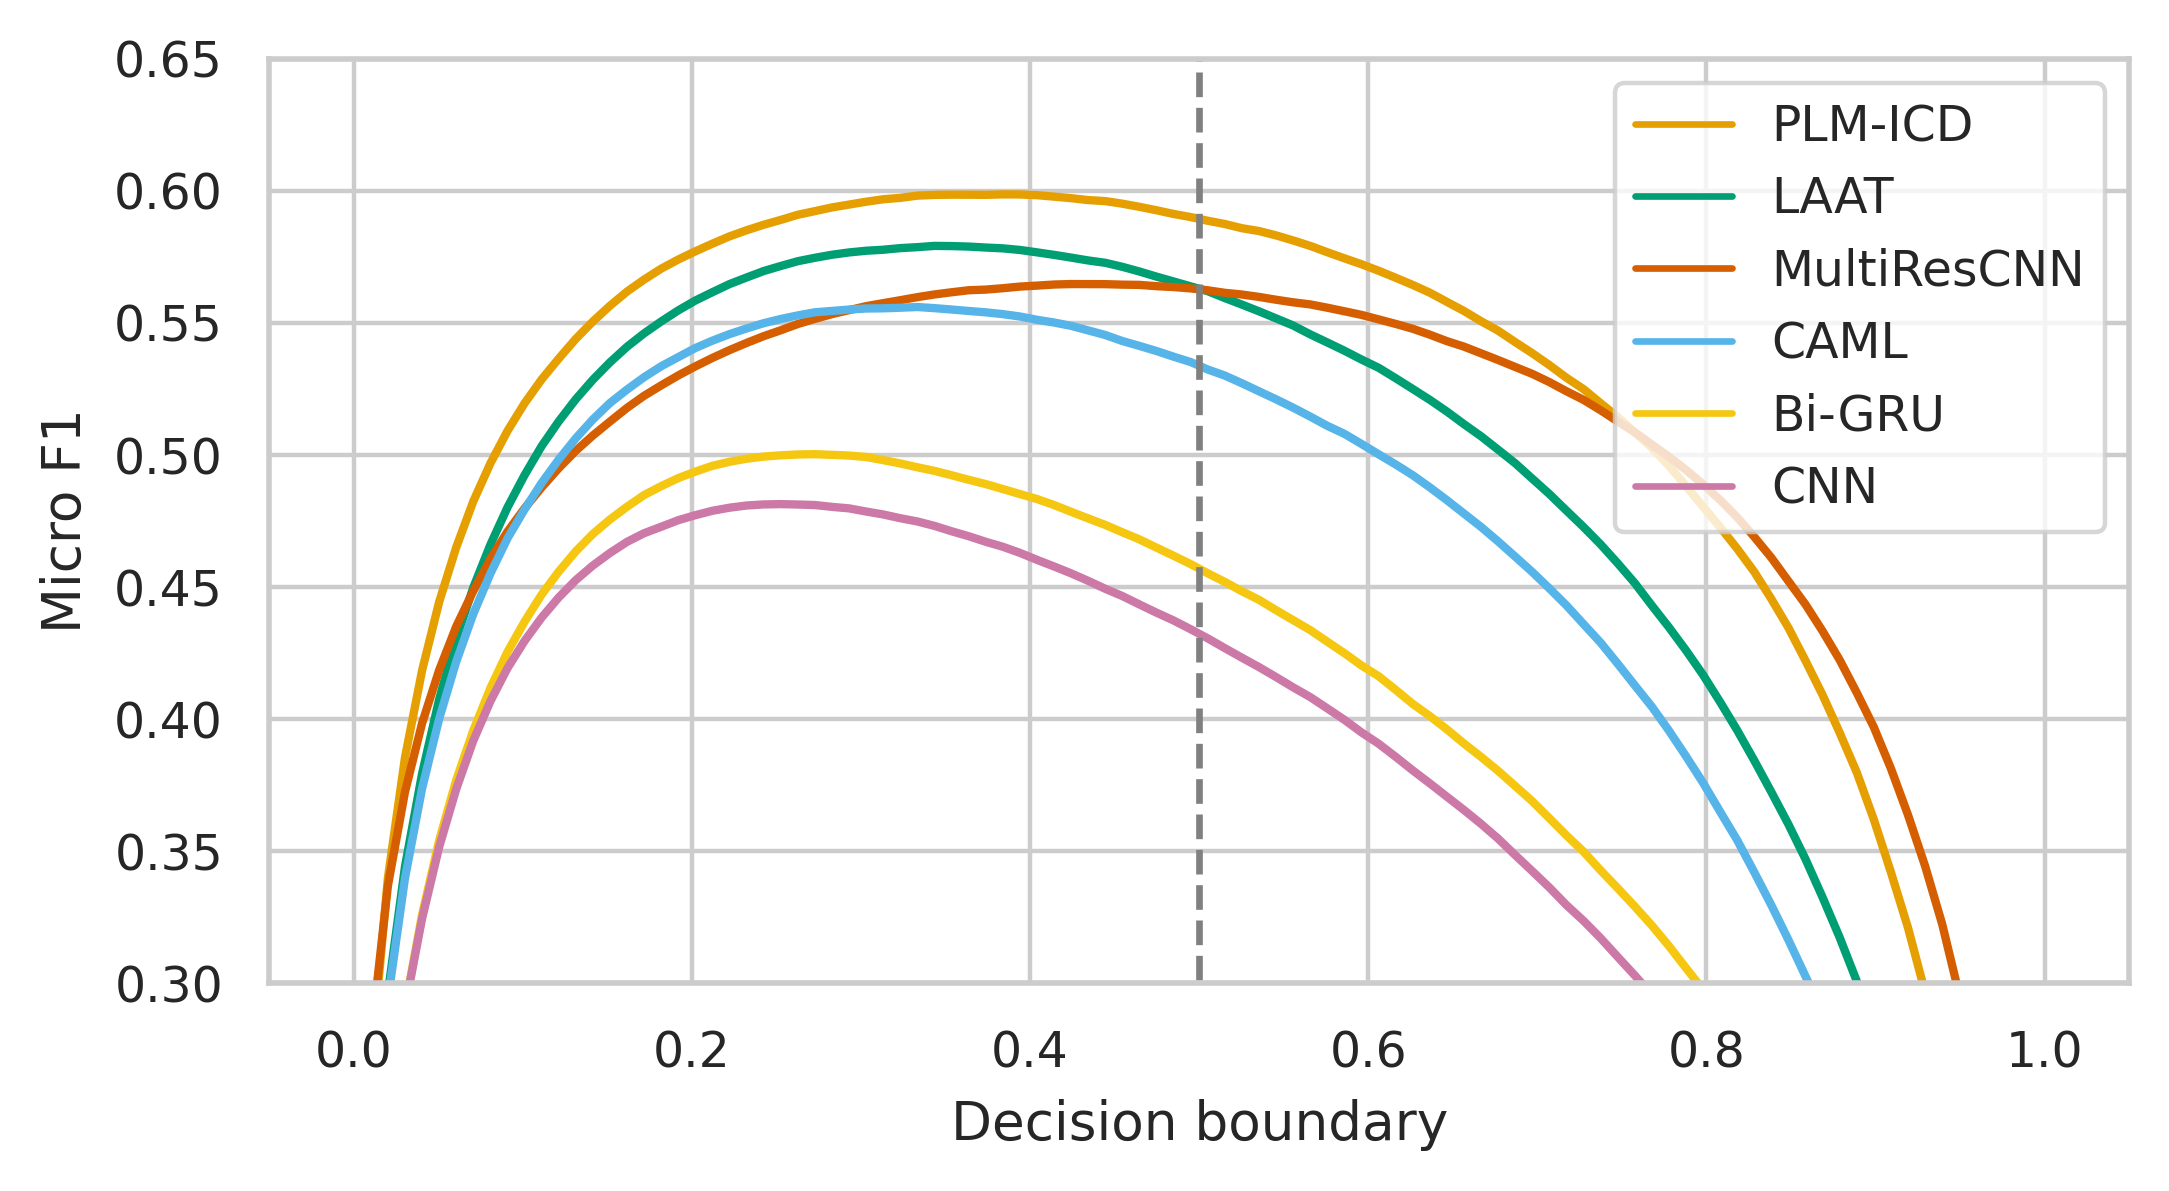
\includegraphics[width=\textwidth]{paper_automated/threshold_tuning_micro_full.png}
        % \caption{}
        % \label{fig:threshold_tuning_micro}
    \end{subfigure}
    \begin{subfigure}[b]{0.9\textwidth}
        \centering
        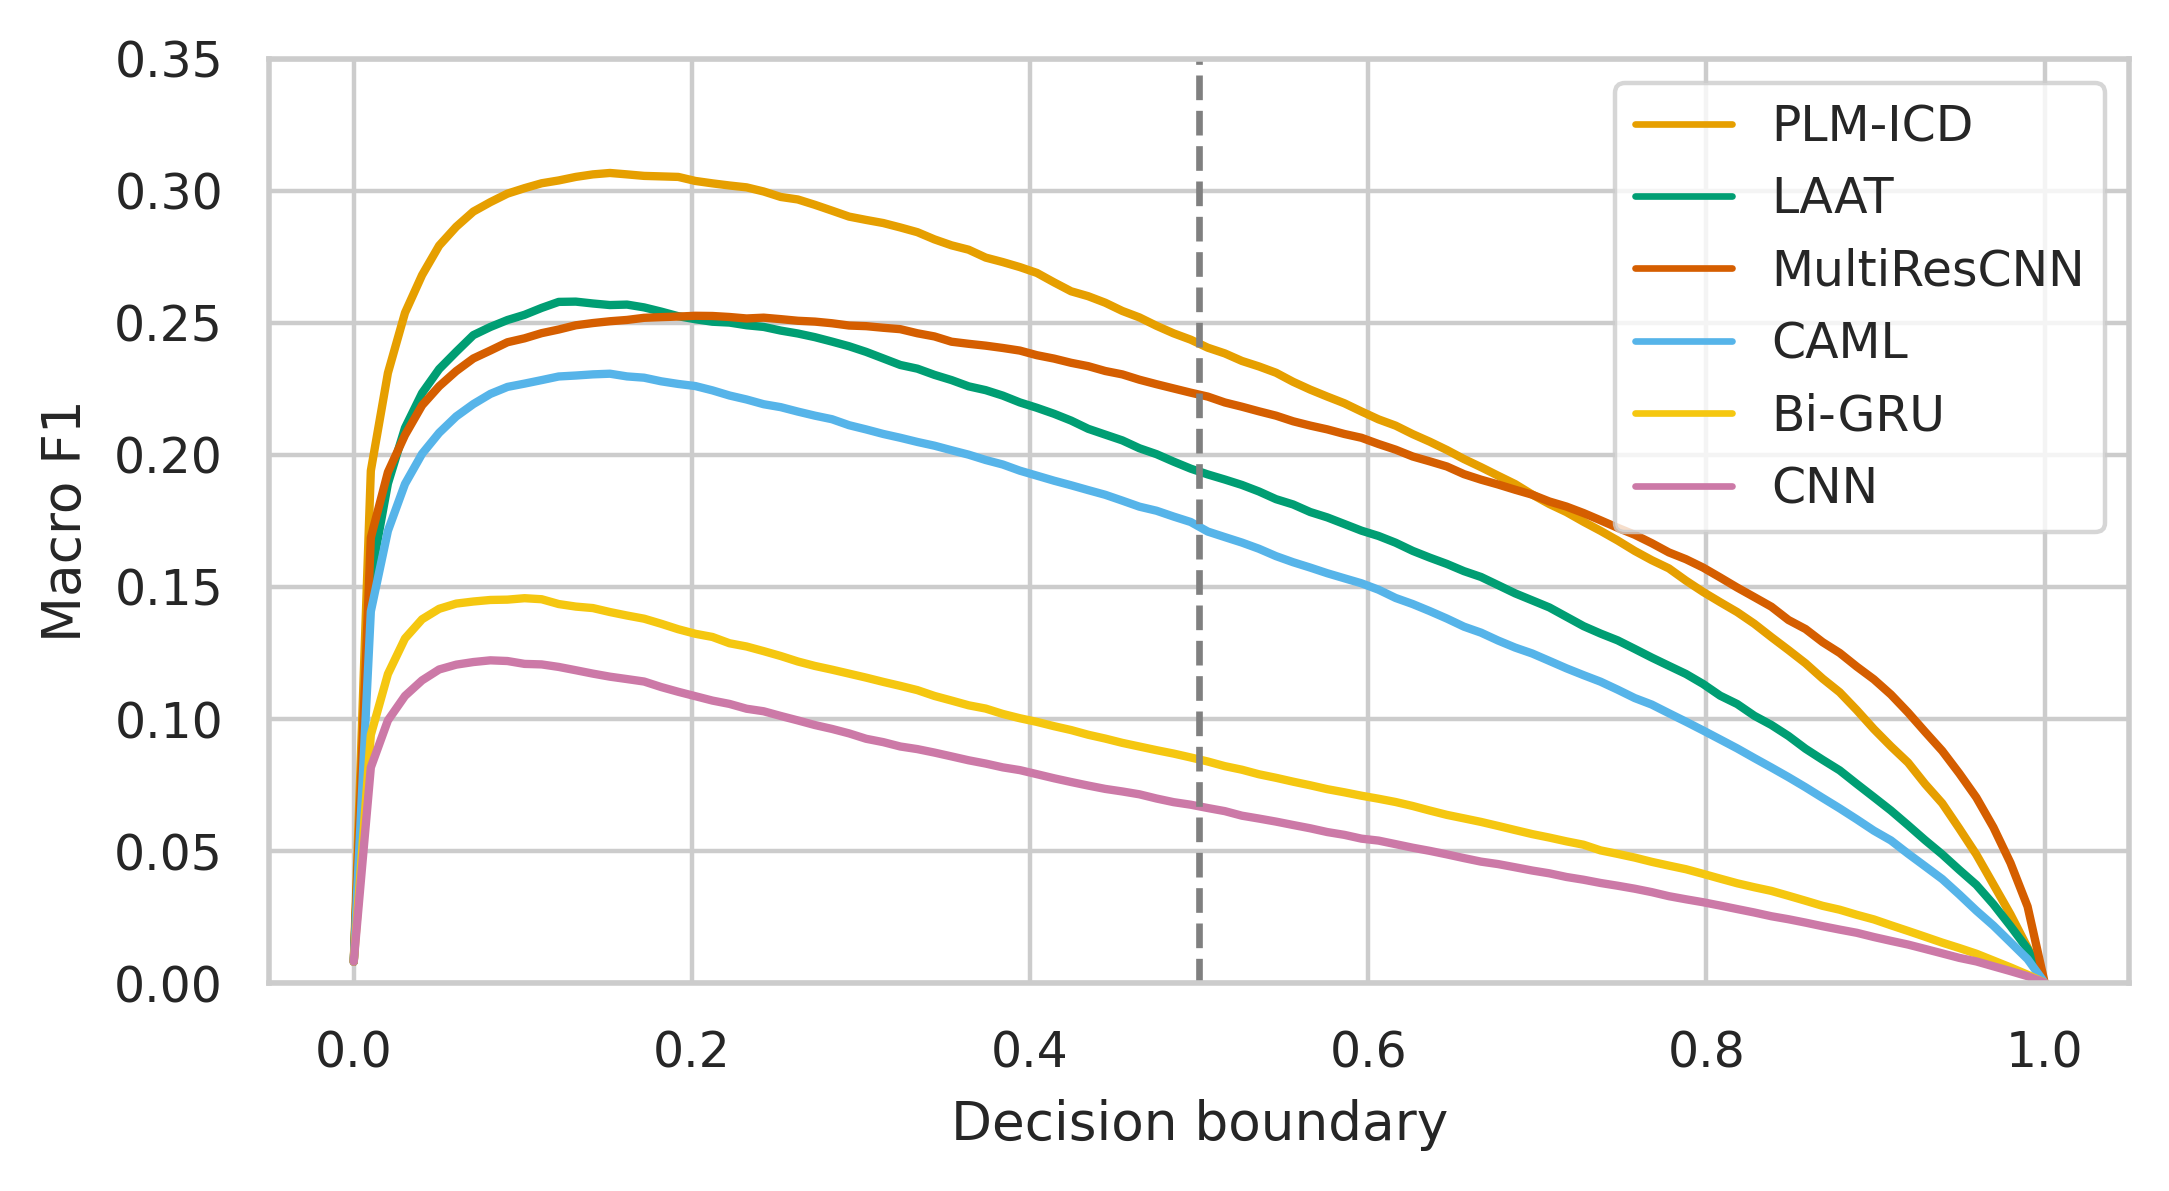
\includegraphics[width=\textwidth]{paper_automated/threshold_tuning_macro_full.png}
        % \caption{}
        % \label{fig:threshold_tuning_macro}
    \end{subfigure}%
    \caption[Relationship between chosen threshold and F1-score of every reproduced model.]{ The relationship between chosen threshold and F1-score of every reproduced model in \cref{tab:reproduced_results}. The left figure shows the micro F1-score, and the right shows the macro F1-score. The models were evaluated on MIMIC-III \textit{clean}.}
    \label{fig:threshold_tuning}
\end{figure}


\subsection{Error analysis}

\paragraph{Amount of training data:}

\cref{fig:train_size} shows the relationship between the number of training examples and the micro and macro F1-scores for all models.
In most cases, increasing the training data had a larger effect on the macro F1-score than the micro F1-score, indicating more extensive improvements in rare codes than common codes. The curve for macro F1 is less smooth because the decision boundary was tuned on the micro F1-scores.

\begin{figure}
    \centering
    \begin{subfigure}[b]{0.95\textwidth}
        \centering
        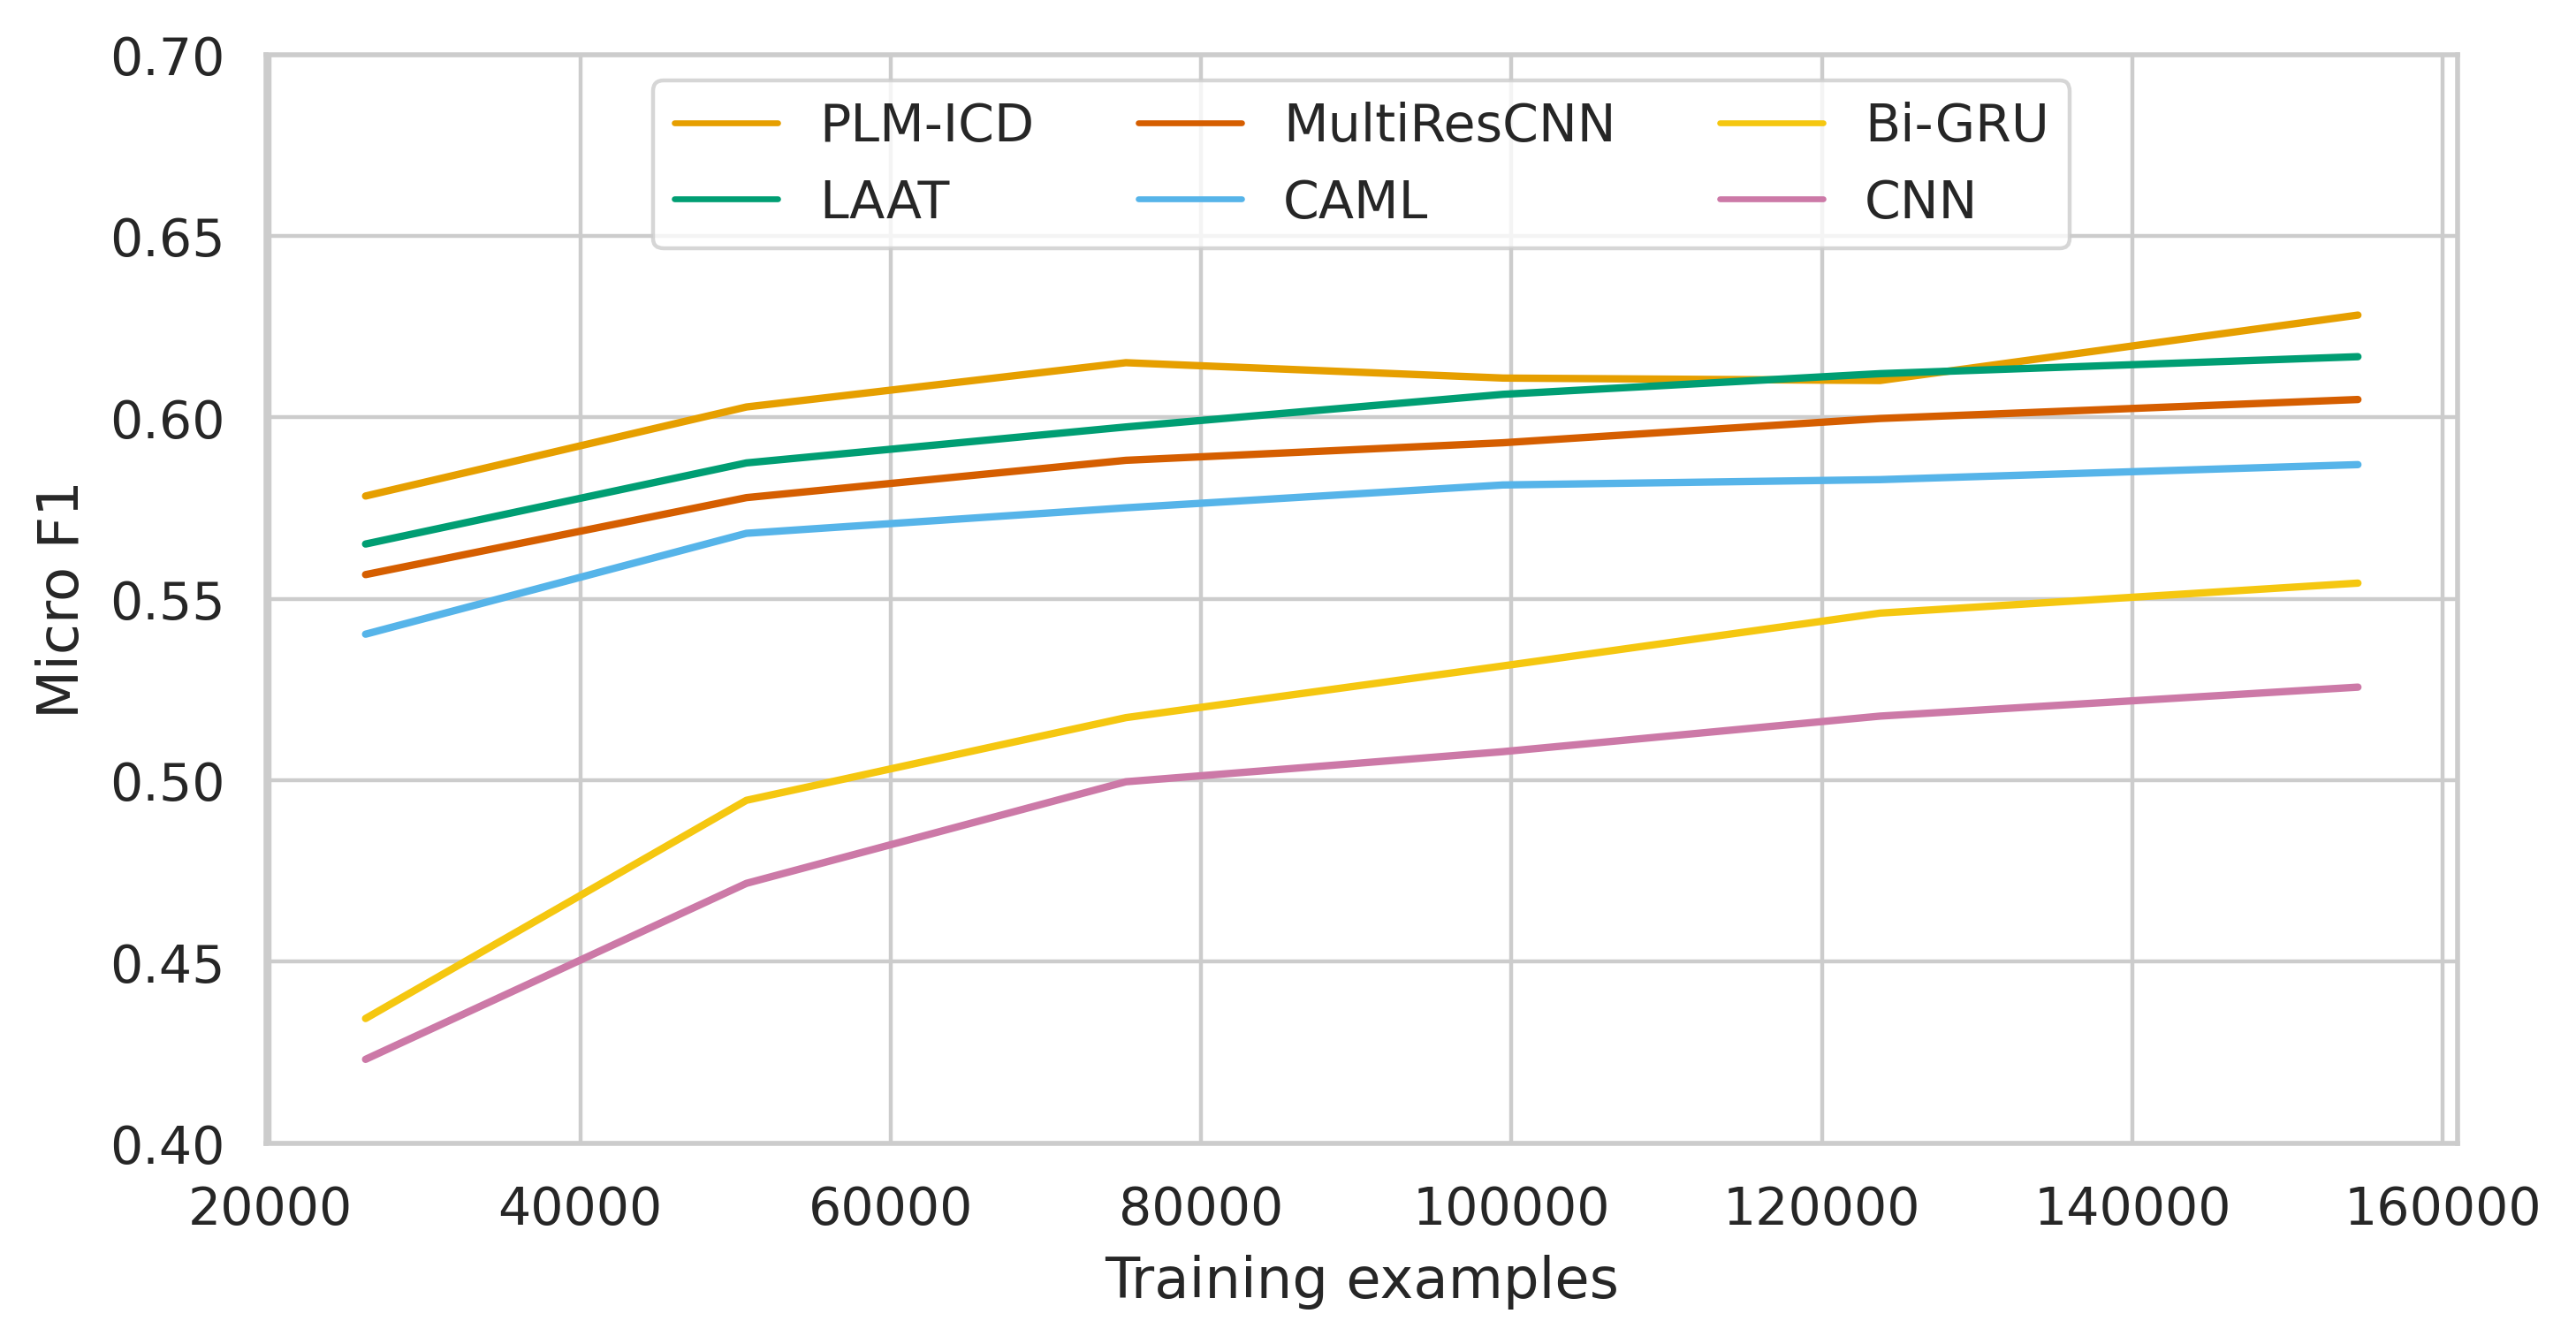
\includegraphics[width=\textwidth]{paper_automated/train_size_f1_micro.png}
        % \caption{}
        % \label{fig:train_size_micro}
    \end{subfigure}
    \begin{subfigure}[b]{0.95\textwidth}
        \centering
        \includegraphics[width=\textwidth]{paper_automated/train_size_f1_macro.png}
        % \caption{}
        % \label{fig:train_size_macro}
    \end{subfigure}
    \caption[The relationship between the number of training examples and F1-score on MIMIC-IV \textit{ICD-9}.]{  The relationship between the number of training examples and F1-score on MIMIC-IV \textit{ICD-9}. The left figure shows the F1 Micro score on the y-axis, while the right figure shows the F1 Macro score.}
    \label{fig:train_size}
\end{figure}


\paragraph{Document length:}\label{subsubsec:document-length}

We plot the micro F1-score for all models as a function of the number of words per document in \cref{fig:text_length}. 
We note that all models underperformed on documents with fewer than 1000 words. 
By manual inspection, we found that most of these documents missed the information necessary to predict their labeled codes, leading to underperformance. 
In \cref{tab:correlations}, we list the Pearson and Spearman correlations. We excluded documents shorter than 1000 words to avoid confounding with missing information and longer than 4000 words due to the truncation limit. We observe a very small negative correlation between document length and micro F1 which matches the downward trend in micro F1, starting from approximately 1000 words in \cref{fig:text_length}. 
Although document length may itself be the cause of the slightly lower performance for long documents, there may be other factors correlated with document length impacting performance, such as the number of codes per document and code frequency.
As there are few long documents, the effect on average micro F1 for each dataset is negligible; hence, previous claims that long documents lead to poor performance in AMC could not be validated. Results on MIMIC-IV \textit{ICD-10} and MIMIC-III \textit{clean} were similar.

\begin{figure}
    \centering
    \includegraphics[width=0.9\textwidth]{paper_automated/f1_micro_vs_num_words.png}
    \caption[Relationship between the lengths of the clinical notes and the micro F1-score for each model on MIMIC-IV \textit{ICD-9}.]{Relationship between the lengths of the clinical notes and the micro F1-score for each model on MIMIC-IV \textit{ICD-9}. The vertical line indicates the maximum length of the notes after truncation. The histogram at the top visualizes the document length distribution.}
    \label{fig:text_length}
\end{figure}

\begin{table}
    \centering
    \caption[Correlation between the F1-score and the logarithm of code frequency and document length on MIMIC-IV \textit{ICD-9}.]{ Correlation between the F1-score and the logarithm of code frequency and document length on MIMIC-IV \textit{ICD-9}. As discussed in \cref{subsubsec:document-length}, we only considered document lengths between 1000 and 4000 words. All correlations are statistically significant ($p<0.001$).}
    \label{tab:correlations}
    \begin{tabular}{lcccc}
        \toprule
        & \multicolumn{2}{c}{Code frequency} & \multicolumn{2}{c}{Document lengths}\\
        \cmidrule(lr){2-3}\cmidrule(lr){4-5}
        & Pearson & Spearman & Pearson & Spearman \\
        \midrule
        CNN  & 0.61 & 0.68 & -0.09 & -0.08 \\
        Bi-GRU & 0.57 & 0.65 & -0.08 & -0.07 \\
        CAML & 0.56 & 0.60 & -0.03 & -0.03   \\
        MultiResCNN & 0.47 & 0.53 & -0.02 & -0.03  \\
        LAAT & 0.52 & 0.57 & -0.02 & -0.02 \\
        PLM-ICD & 0.48 & 0.52 & -0.02 & -0.02   \\
        \bottomrule
    \end{tabular}
\end{table}


\paragraph{Code analysis:}

\Cref{fig:icd9_vs_icd10} compares the best performing model, PLM-ICD, trained and evaluated on MIMIC-IV \textit{ICD-9} and \textit{ICD-10}. Similar results were obtained on MIMIC-III \textit{clean}.
The comparison shows the relationship between code frequencies in the training set and macro F1-scores. As shown in \cref{tab:fair_results}, all models perform worse on \textit{ICD-10} compared to \textit{ICD-9}. However, \cref{fig:icd9_vs_icd10} demonstrates that performance on codes with similar frequencies is comparable between the two splits. This suggests that the performance differences in \cref{tab:fair_results} are due to \textit{ICD-10} containing a higher fraction of rare codes as shown in \cref{fig:mimiciv_code_dist,fig:icd9_vs_icd10}.

The Pearson and Spearman correlations between the logarithm of code frequency and F1-score are shown in \cref{tab:correlations} for MIMIC-IV \textit{ICD-9}. Similar correlations were observed for the other datasets. All the models show moderately high correlation confirming that performance on rare codes is generally lower than on common codes. To further our understanding of the problem, we computed the percentage of unique codes in each dataset that the models never predicted. As seen in \cref{tab:missed_classes}, no model correctly predicted more than 50\% of the ICD-10 codes.

\Cref{fig:chapter_performance} shows the performance of PLM-ICD on each ICD-10 chapter---the top-most level in the tree-like hierarchy. 
For our analysis, we limited the scope to only focus on the diagnosis codes. We also excluded codes with fewer than one hundred training examples to control for some chapters having many rare codes. 

Overall, PLM-ICD never correctly predicted 2,928 of the 5,794 ICD-10 diagnosis codes in our split. Of these codes, only 110 had over a hundred training examples, and 58 belong to only two of the 20 chapters in MIMIC-IV \textit{ICD-10}. Specifically, 45 belong to the chapter relating to ``external causes of morbidity" (Z00-Z99), while 13 relate to ``factors influencing health status and contact with health services" (V00-Y99). To further investigate why most non-predicted codes with more than 100 training examples belong to only two chapters, we manually inspected a selection of codes in these chapters, as described in the following.

The Z68 category, part of the Z00-Z99 chapter, contains codes related to the patient's body mass index (BMI). Codes within this category occur more than 17,000 times in the MIMIC-IV training data, but PLM-ICD never predicts 20 out of the 26 codes of Z68. One possible hypothesis is that PLM-ICD struggles with extracting the BMI from the discharge summaries, as all digits have been removed in the pre-processing. We found several other codes containing digits in the code descriptions that the model failed to detect, e.g., ``Blood alcohol level of less than 20 mg/100 ml" (Y90.0), ``34 weeks gestation of pregnancy" (Z3A.34), and ``NIHSS score 15" (R29.715). These observations support our hypothesis that removing digits in the pre-processing makes certain codes challenging to predict.

The Y92 category, part of the V00-Y99 chapter, contains codes related to the physical location of occurrence of the external cause. It is a large category of 246 unique codes occurring 27,870 times in the training set. The category is challenging due to locations being very specific. For instance, there are unique codes for whether an incident occurred on a tennis court, squash court, art gallery, or museum. We hypothesize that the level of detail in the discharge summaries does not always match the fine-grained code differences.

\begin{figure}
    \centering
    \includegraphics[width=0.9\textwidth]{paper_automated/code_count_vs_f1_all_datasets.png}
    \caption[Relationship between code frequencies and macro F1-score for PLM-ICD on MIMIC-IV \textit{ICD-9} and \textit{ICD-10}.]{Relationship between the code frequencies in the training set and the macro F1-score for PLM-ICD on MIMIC-IV \textit{ICD-9} and \textit{ICD-10}. The shaded area indicates the standard deviation of the score computed for codes within the bin.}
    \label{fig:icd9_vs_icd10}
\end{figure}

There are ten different codes in MIMIC-IV \textit{ICD-10} relating to nicotine dependence and tobacco use. The three most common are Z87.891 (``Personal history of nicotine dependence"), F17.210 (``Nicotine dependence, cigarettes, uncomplicated"), and Z72.0 (``Tobacco use"), with 26,427, 8,486, and 1,914 training examples, respectively. Among these, Z72.0 was the third most common single code in the training set that PLM-ICD never predicted correctly. PLM-ICD achieved an F1-score of 53\% for Z87.891, 51\% for F17.210, and 0\% for Z72.0 and all other nicotine-related codes. These findings suggest that when there is a class imbalance among highly similar codes, PLM-ICD is strongly biased toward the most frequent ones.

 \begin{table}
    \centering
    \caption{Percentage of ICD diagnosis codes in the test set that the models never predicted correctly.}
    \label{tab:missed_classes}
    \begin{tabular}{lccc}
        \toprule
        & MIMIC-III & \multicolumn{2}{c}{MIMIC-IV}\\
        \cmidrule(lr){2-2}\cmidrule(lr){3-4}
        & \textit{clean} &  \textit{ICD-9} & \textit{ICD-10} \\
        \midrule
        CNN  & 68.2 & 61.5 & 72.0\\
        Bi-GRU  & 65.0 & 54.3 & 67.1\\
        CAML & 52.8 & 57.0 & 62.0  \\
        MultiResCNN  & 48.8 & 40.3 & 53.5 \\
        LAAT  & 50.4 & 43.6 & 55.0\\
        PLM-ICD   & 44.3 & 39.3 & 51.8\\
        \bottomrule
    \end{tabular}
\end{table}


\begin{figure}
    \centering
    \includegraphics[width=0.9\textwidth]{paper_automated/chapters.png}
    \caption[Performance of PLM-ICD on ICD-10 chapters.]{Performance of PLM-ICD on ICD-10 chapters. Only codes with more than a hundred occurrences in the MIIMC-IV ICD-10 training set were considered, leaving 20 chapters. We found Z00-Z99 and V00-Y99 to be the most challenging.}
    \label{fig:chapter_performance}
\end{figure}




\section{Discussion}
\subsection{Lessons learned}
We found reproducing the results of CNN, Bi-GRU, CAML, and LAAT challenging. While we expected discrepancies due to random weight initializations and data shuffling, the differences from the original works exceeded our presuppositions. Our reproduced results were better than originally reported for Bi-GRU and CNN and worse for CAML and LAAT on most metrics. There have been multiple reports of issues in reproducing the results of \textcite{mullenbachExplainablePredictionMedical2018}.\footnote{\url{https://github.com/jamesmullenbach/caml-mimic}} Additionally, most previous works did not report which version of MIMIC-III they used, and the code and hyperparameter configurations were not documented in detail. Therefore, we hypothesize that our results differ because previous works report incorrect hyperparameters or use an earlier version of MIMIC-III.

We showed that models previously reported as low-performing underperformed partly due to a poor selection of hyperparameters and not tuning the decision boundary. In our revised comparison, we demonstrated that training the models using our setup decreased the difference between the best and worst micro F1-scores by $5.8$ percentage points. \textcite{mullenbachExplainablePredictionMedical2018} concluded that CNN outperformed Bi-GRU. However, in our revised comparison, Bi-GRU outperformed CNN on all metrics on MIMIC-III \textit{clean}, MIMIC-IV \textit{ICD-9}, and MIMIC-IV \textit{ICD-10}.

Even though MultiResCNN contains more parameters than CAML, \textcite{liICDCodingClinical2020} concluded that MultiResCNN was faster to train because it converged in fewer epochs. However, this was only true when using the original setup where CAML converged after 84 epochs. We found that when using a learning rate schedule and appropriate hyperparameters, it was possible to train all the models in 20 epochs without sacrificing performance. Therefore, with our setup, CAML was faster to train than MultiResCNN.

We demonstrated that the macro F1-score had been underestimated in prior works due to the poorly sampled MIMIC-III \textit{full} split and the practice of setting the F1-score of all codes absent in the test set to 0. Since 54\% of the codes in MIMIC-III \textit{full} are missing in the test set, the maximum possible macro F1-score is 46\%. The previously highest reported macro F1-score on MIMIC-III \textit{full} is 12.7\% for PLM-ICD~\parencite{kimReadAttendCode2021}. Using our corrected macro F1-score on the same split, PLM-ICD achieved a macro F1-score of 22.8\%. This large difference from previous state-of-the-art seems to indicate that all previous work on AMC used the suboptimally calculated macro F1-score, including works not reproduced in this paper. Many studies use the macro F1-score to evaluate the ability of their models to predict rare codes \parencite{kimReadAttendCode2021, yuanCodeSynonymsMatter2022}. If it has indeed been incorrectly calculated in these studies, some conclusions drawn in previous work regarding rare code prediction may have been misguided.

Multiple studies mention lack of training data, rare codes, and long documents as the main challenges of AMC \parencite{dongExplainableAutomatedCoding2021,feuchtDescriptionbasedLabelAttention2021,huangPLMICDAutomaticICD2022,jiDoesMagicBERT2021,liICDCodingClinical2020,liuEffectiveConvolutionalAttention2021,moonsComparisonDeepLearning2020,pascualBERTbasedAutomaticICD2021,tengReviewDeepNeural2022,tengExplainablePredictionMedical2020, vuLabelAttentionModel2020, venkateshAutomatingOverburdenedClinical2023}. In the error analysis, we aimed to validate or falsify these assumptions. We found that rare codes were challenging for all models and observed that more than half of all ICD-10 codes were never predicted correctly. Furthermore, in \cref{fig:train_size}, we showed that when adding more training data, most models see a greater performance improvement on rare codes than on common codes. 
These findings suggest that medical coding is fundamentally challenged by a lack of training data that, in turn, gives rise to many rare codes.
We found that document length and model performance only exhibited a weak correlation. Specifically, the low number of very long documents was insufficient to affect the average performance on the dataset. 

\subsection{Future work}
We recommend future work within AMC use our revised comparison method, including stratified sampled splits of MIMIC datasets, corrected evaluation metrics, hyperparameter search, and decision boundary tuning to avoid reporting suboptimal or biased results. 
Furthermore, for AMC to become a viable solution for ICD-10, future research should focus on improving performance on rare codes while, in the shorter term, developing methods to detect codes that are too challenging for automated coding and, therefore, should be coded manually. Finally, while PLM-ICD outperforms the other models in this paper, the improvements are limited compared to the effect of pre"=training in other domains \parencite{mohamed_selfsupervised_2022, linPretrainedTransformersText2021,baevski_wav2vec_2020,devlin_bert_2018,dosovitskiy_image_2021}.
Notably, there have been several unsuccessful attempts at using pre"=trained transformers for medical coding \parencite{jiDoesMagicBERT2021,gaoLimitationsTransformersClinical2021,michalopoulosICDBigBirdContextualEmbedding2022,pascualBERTbasedAutomaticICD2021,zhangBERTXMLLargeScale2020}. In future work, we want to investigate why pre"=trained transformers underperform in medical coding.


\subsection{Limitations}
We presented findings and analyses on MIMIC-III and MIMIC-IV. It is unclear how our findings generalize to medical coding in real-world settings.
For instance, since MIMIC-III and IV contain data from the emergency department and ICU of a single hospital, the findings in this paper may not generalize to other departments or hospitals. 
For instance, discharge summaries from outpatient care are often easier to code than summaries from inpatient care as they are shorter with fewer codes per document \parencite{zhangBERTXMLLargeScale2020, liuEffectiveConvolutionalAttention2021, tsengAdministrativeCostsAssociated2018}.

The medical code labeling of MIMIC is used as a gold standard in this paper. However, medical coding is error-prone, and, in many cases, deciding between certain codes can be a subjective matter \parencite{nouraeiAuditNatureImpact2013, lloydPhysicianCodingErrors1985}. \textcite{burnsSystematicReviewDischarge2012} systematically reviewed studies assessing the accuracy of human medical coders and found an overall median accuracy of 83.2\% (IQR: 67.3–92.1\%). \textcite{searleExperimentalEvaluationDevelopment2020} investigated the quality of the human annotations in MIMIC-III and concluded that 35\% of the common codes were under-coded. Such errors and subjectivity in manual medical coding make model training and evaluation challenging and suggests that additional evaluation methods using, e.g., a human-in-the-loop, could be useful to increase the reliability of results. 

\section{Conclusion}
In this paper, we first reproduced the results of selected state-of-the-art models focusing on unimodal models with publically available source code. 
We found that model evaluation in original works was biased by an inappropriate formulation of the macro F1-score and treatment of missing classes in the test set. By fixing the macro F1 computation, we approximately doubled the macro F1 of the reproduced models on MIMIC-III \textit{full}. 
We introduced a new \textit{clean} split for MIMIC-III that contains all classes in the test set and performed a revised comparison of all models under the same training, evaluation, and experimental setup, including hyperparameter and decision boundary tuning. We observed a significant performance improvement for all models, with those previously reported as low-performing improving the most. 
We reported the first results of current state-of-the-art models on the newly released MIMIC-IV dataset \parencite{johnsonMIMICIVFreelyAccessible2023, goldbergerPhysioBankPhysioToolkitPhysioNet2000} and provided splits for the \textit{ICD-9} and \textit{ICD-10} coded subsets using the same method as for MIMIC-III \textit{clean}.
Through error analysis, we provided empirical evidence for multiple model weaknesses. Specifically, models underperform severely on rare codes 
and, in contrast to previous claims, long documents only have a negligible negative performance impact. 
We release our source code, model parameters, and the new MIMIC-III \textit{clean} and MIMIC-IV \textit{ICD-9} and \textit{ICD-10} splits.$^(\ref{footnote:source_code})$

\section*{Acknowledgments}
This research was partially funded by the Innovation Fund Denmark via the Industrial Ph.D. Program (grant no. 2050-00040B, 0153-00167B, 2051-00015B) and Academy of Finland (grant no. 322653).
We thank Sotiris Lamprinidis for implementing our stratification algorithm and data preprocessing helper functions.
   
}
  % 8p
% \include{appendices/paper_we}  % 4p
% \include{appendices/paper_multiqt}  % 8p

%!TEX root = ../thesis.tex

\chapter[supplementary material for hierarchical vaes know what they don't know]{Supplementary material for Hierarchical VAEs know what they don't know}
\label{chp:appendix-hierarchical}
\ifthenelse{\equal{\skipappendices}{true}}{}{

\section{Datasets}
\cref{tab_hierarchical:datasets-overview} lists the datasets used in the paper. We use the predefined train/test splits for the datasets.

For SmallNORB and Omniglot we resize the original grey-scale images to $28\times28$ with ordinary bi-linear interpolation.
For each of these datasets, we also create a version where the grey-scale is inverted. We do this because, the overall white nature of the images tends to make detecting them as OOD from FashionMNIST artificially easy.
The inversion is done via the simple transformation $\xb_\text{inverted} = 255 - \xb_\text{original}$ since images are encoded as 8 bit unsigned integers.

% Similar to \citet{serra_input_2020} and \citet{xiao_likelihood_2020}, we also create a uniform noise dataset ``UniformNoise'' and benchmark our model against this. We dynamically sample each pixel value uniformly as an integer between 0 and 255.

\begin{table}[h!]
    \centering
    % \resizebox{0.7\columnwidth}{!}{%
    \begin{tabular}{llr}
        \toprule
        Dataset & Dimensionality & Examples \\
        \midrule
        FashionMNIST \cite{xiao_fashionmnist_2017} & $28\times28\times1$ & 70,000 \\
        MNIST \cite{lecun_gradientbased_1998} & $28\times28\times1$ & 70,000 \\
        notMNIST \cite{bulatov_notmnist_2011} & $28\times28\times1$ & 547,838 \\
        KMNIST \cite{clanuwat_deep_2018} & $28\times28\times1$ & 70,000 \\
        Omniglot \cite{lake_humanlevel_2015} & $28\times28\times1$ & 32,460 \\
        SmallNORB \cite{lecun_learning_2004} & $28\times28\times1$ & 97,200 \\
        % UniformNoise & $28\times28\times1$ & dynamic \\
        \midrule
        CIFAR10 \cite{krizhevsky_learning_2009} & $32\times32\times3$ & 60,000 \\
        SVHN \cite{netzer_reading_2011} & $32\times32\times3$ & 99,289 \\
        \bottomrule
    \end{tabular}
    % }
    \caption{Overview of the used datasets.}
    \label{tab_hierarchical:datasets-overview}
\end{table}


\section{Model details}\label{sec:model-details}
In \cref{tab_hierarchical:hyperparameters} we specify the hyperparameters used when training our models.
We make our source code available at \url{https://github.com/JakobHavtorn/hvae-oodd}.

\subsection{Hierarchical VAE}
Our Hierarchical VAE (HVAE) model uses bottom-up inference and top-down generative paths as specified in the paper.
For grey-scale images, the output is parameterized by a Bernoulli distribution while for natural images we use a Discretized Logistic Mixture \cite{salimans_pixelcnn_2017}.
The latent variables are parameterized by stochastic layers that output the mean and log-variance of a diagonal covariance Gaussian. The prior distribution on the top-most latent is a standard Gaussian.
For grey-scale images, the lowest latent space is parameterized by a convolutional neural network and has dimensions $14\times14\times8$ interpreted as (height $\times$ width $\times$ latent dimension). The highest two latent variables are parameterized by dense transformations with $16$ and $8$ units, respectively.
For natural images, the bottom-two latent variables are parameterized by convolutional neural networks and have dimensions $(16\times16)\times128$, $(8\times8)\times64$, respectively for $\zb_1, \zb_2$. The top-most latent, $\zb_3$, is densely connected with dimension $32$.

Each stochastic layer is preceeded by a determininistic transformation.
For both grey-scale and natural images, each deterministic transformation consists of three residual blocks of the same type used by \textcite{maaloe_biva_2019}. The structure of a residual block is:
\begin{equation}
    \yb = \textsc{conv}\left( \textsc{act} \left( \textsc{conv}_s \left( \textsc{act}(\xb) \right) \right) \right) + \xb \ ,
\end{equation}
where \textsc{conv} refers to a same-padded convolution and \textsc{act} to the activation function. Within a residual block, the first convolution always has stride 1 while the second convolution has stride $s$. In a deterministic transformation, any non-unit stride is performed in the third residual block. For grey-scale images, we stride by 2 in the first and second deterministic transformations but not the third. For natural images, we similarly stride by 2 in the first and second deterministic transformations. For grey-scale we use 64 channels while we use 256 for natural images.
In both cases, the first deterministic block uses a kernel size of 5 and the latter two a kernel of size 3. We use the ReLU activation function \cite{fukushima_neocognitron_1980, nair_rectified_2010}.

Since the benefits and drawbacks of using batch normalization \cite{ioffe_batch_2015} in hierarchical VAEs is still the matter of some debate \cite{sonderby_ladder_2016, vahdat_nvae_2020, child_very_2021} we choose to use weight normalization \cite{salimans_weight_2016} as in other work \cite{maaloe_biva_2019} and initialize the model using the originally proposed data-dependent initialization.
To have the stochastic layers initialize to standard Gaussian distributions (zero mean, unit variance), with this initialization, we select the activation function for the variance as a Softplus,
\begin{equation*}
    \textsc{softplus}(\xb) = \frac{1}{\beta}\log\left(1 + \exp(\beta\xb)\right) \ ,
\end{equation*}
with $\beta = \log(2) \approx 0.693$ to output 1 for $\xb = 0$.

Training of a HVAE model took approximately two days on a single NVIDIA GTX 1080 Ti graphics card.


\subsection{BIVA}
For the BIVA model \cite{maaloe_biva_2019}, we use a specification that is very similar to that of the HVAE above, and to that of the original paper.
The model has 10 latent variables the lowest 3 of which are spatial and the rest are densely connected in order to have an architecture similar to the HVAE.
The model uses an overall stride of 8, achieved by striding by 2 in the first, fourth and sixth deterministic transformations.
From $\zb_1$ to $\zb_{10}$, the latents have the following dimensions: The lowest three latents are spatial $(16\times16)\times8$, $(16\times16)\times16$ and $(16\times16)\times32$, given as $(\text{height}\times\text{width})\times\text{dim})$, while the rest are dense vectors with dimensions of $42, 40, 38, 36, 34, 32, 30$.

Training of a BIVA model took approximately a week on a single NVIDIA GTX 1080 Ti graphics card.


\begin{table}[h]
    \centering
    % \resizebox{\columnwidth}{!}{%
    \begin{tabular}{ll}
        \toprule
        Hyperparameter & Setting/Range \\
        \midrule
        \multicolumn{2}{l}{\textbf{All}} \\
        \midrule
        Optimization & Adam \cite{kingma_adam_2015} \\
        Learning rate & $3e-4$ \\
        Batch size & 128 \\
        Epochs & 2000 \\
        Free bits & $\SI{2}{nats}$ per $\zb_i$ shared across latent dim. \\
        Free bits constant & 200 epochs \\
        Free bits annealed & 200 epochs \\
        Activation & ReLU \\
        \multirow{2}{*}{Initialization} & Data-dependent \\
        & \cite{salimans_weight_2016} \\
        \midrule
        \multicolumn{2}{l}{\textbf{HVAE}} \\
        Latent dimensionality & 128-64-32 (natural) / 8-16-8 (grey) \\
        Convolution kernel & 5-3-3 \\
        Stride & 2-2-1 \\
        Warmup anneal period & 200 epochs \\
        \midrule
        \multicolumn{2}{l}{\textbf{BIVA}} \\
        \multirow{2}{*}{Latent dimensionality} & 10-8-6 (spatial) \\
        & 42-40-38-36-34-32-30 (dense) \\
        Convolution kernel & 5-3-3-3-3-3-3-3-3-3 \\
        Stride & {2-1-1-2-1-2-1-1-1-1} \\
        \bottomrule
    \end{tabular}
    % }
    \caption[Selection of most important hyperparameters]{Selection of most important hyperparameters and their setting. Convolutional kernels are square and latent dimensions are given without spatial dimensions which are given in the text. See \cref{sec:model-details} for more details.}
    \label{tab_hierarchical:hyperparameters}
\end{table}


\section{Analysis of the influence of latent variables on the marginal likelihood}
In the paper, we argue that the lowest level latent variables, which have the highest dimensionality, contribute the most to the approximate likelihood.
Here, we provide a stringent mathematical argument that generalizes this to the exact marginal likelihood in a model with a deterministic decoder.

\subsection{Model specification}
For an arbitrary hierarchical latent variable model, we have a prior $p(\zb_L)$ and a generative mapping $f: \mathbb{R}^d \rightarrow \mathbb{R}^D$, such that $\xb = f(\zb_L)$ and $D>d$.
Note that we will assume that $f$ is deterministic, such that we are effectively working with $p(\xb|\zb) = \delta_{f(\zb)}(\xb)$.
This is a limiting assumption, but it allows working through the following. For shorthand we will simply write $\zb=\zb_L$.

Let $f$ have a bottleneck architecture, i.e.\
\begin{align}
f(\zb) &= f_1(\ldots f_{L-1}(f_L(\zb))) \ ,
\end{align}
where
\begin{align}
    f_i: \mathbb{R}^{d_{i}} \rightarrow \mathbb{R}^{d_{i-1}}, \qquad i = L, \ldots, 1 \ .
\end{align}
Here we use the notation $d_0=D=\vert\xb\vert$ and $d_L=d=\vert\zb\vert$ and further assume $d_0\geq d_1\geq \ldots \geq d_{L-1} \geq d_L$ which gives the bottleneck.
%$d_1 = d$ and $d_{L+1} = D$ and further assume $d = d_1 \leq d_2 \leq \ldots \leq d_L \leq d_{L+1} = D$ which gives the bottleneck.

Assuming $\xb$ is such that a corresponding latent variable $\zb$ exists, i.e.\ that there exists $\zb$ such that $\xb = f(\zb)$, then we can write the likelihood of $\xb$ through a standard change of variables (similar to flow-based models),
\begin{align}
    p(\xb) &= p(\zb) \prod_{i = 1}^L \left(\sqrt{\det \Jb_i^T \Jb_i}\right)^{-1} \ ,
\end{align}
where $\Jb_i$ is the Jacobian of $f_i$, i.e.
\begin{align}
    \Jb_i &= \frac{\partial f_i}{\partial \zb_i} \in \mathbb{R}^{d_i\times d_{i-1}} \ .
\end{align}
Here we use the notation that $\zb_i$ is the representation at layer $i$.
Note that $\Jb_i^T \Jb_i$ is a $d_{i-1} \times d_{i-1}$ symmetric positive semidefinite matrix (determinant $\geq 0$).

The log-likelihood can be written as
\begin{equation}
    \log p(\xb) = \log p(\zb) - \frac{1}{2} \sum_{i=1}^L \log \det \Jb_i^T\Jb_i \ .
\end{equation}

By construction of determinants, we can generally expect these determinants to grow with the dimensionality of the matrix.
We should expect the determinant of a $d \times d$ matrix to be of the order $\mathcal{O}(\lambda^d)$ for some number $\lambda>0$.
With that in mind, we should generally expect that
\begin{align}
    \det \Jb_{i+1}^T \Jb_{i+1} < \det \Jb_i^T \Jb_i \ ,
\end{align}
due to the bottleneck assumption.
If so, we see that the marginal likelihood $p(\xb)$ will be dominated by $\left(\sqrt{\det \Jb_1^T \Jb_1}\right)^{-1}$, i.e.\ low-level features have a higher influence on the likelihood than more important semantic ones.

\subsection{The Gaussian case}
%
\begin{figure}[t]
    \centering
    \includegraphics[width=\columnwidth]{paper_hierarchical/logdet2.pdf}
    \caption{The expected inverse volume change for Gaussian Jacobians \eqref{eq_hierarchical:Edet} on a log-scale.}
    \label{fig_hierarchical:Edet}
\end{figure}
The previous remarks can be made more precise if we make distributional assumptions on the Jacobians.
Here we will assume that the Jacobians of each layer follow a Gaussian distribution.
Specifically, we will assume that each entry in $\Jb_i$ is distributed as $\mathcal{N}(0, \sigma^2)$.
The analysis below extends to nonzero means and more general covariance structure, but this comes with a cost of less transparent notation.
In this setting, $\Jb_i^T \Jb_i$ follows a Wishart distribution (in the general setting it would follow a non-central Wishart distribution).
\textcite{muirhead_aspects_2009} tells us that the expected multiplicative contribution to the likelihood of each layer is
\begin{align}
    \mathbb{E}\left[ \left(\sqrt{\det \Jb_i^T \Jb_i}\right)^{-1} \right]
    &= \sigma^{-d_{i-1}}  2^{-\frac{d_{i-1}}{2}} \frac{\Gamma_{d_{i-1}}\left( \frac{1}{2} d_{i} - \frac{1}{2} \right)}{\Gamma_{d_{i-1}}\left( \frac{1}{2} d_{i} \right)} \notag \\
    &= \sigma^{-d_{i-1}}  2^{-\frac{d_{i-1}}{2}} \frac{\Gamma\left( \frac{1}{2} (d_{i} - d_{i-1}) \right)}{\Gamma\left( \frac{1}{2} d_{i} \right)}
    \label{eq_hierarchical:Edet}
\end{align}
where $\Gamma_d$ is the multivariate Gamma function.
Assuming that the increase in layer dimension $d_{i} - d_{i-1}$ is constant, then we see that \eqref{eq_hierarchical:Edet} goes to zero as $d_{i}$ goes to infinity as the $\Gamma$ function grows super-exponentially to infinity.
This super-exponential growth further implies that the first layers dominate the marginal likelihood $p(\xb)$.
This is also visually evident in \cref{fig_hierarchical:Edet}.

\section{Derivation of the \texorpdfstring{$\mathcal{L}^{>k}$}{Lk} bound}
In this section we present the derivation of $\mathcal{L}^{>k}$ and show that it is a lower bound on the marginal likelihood.

First, we consider a two-layered VAE with bottom-up inference.
We proceed very similarly to the derivation of the regular ELBO and also use Jensen's inequality.
\begin{align}
\log p(\xb) &= \log \int\int p(\xb|\zb_1)p(\zb_1|\zb_2)p(\zb_2) \text{d}\zb_1\text{d}\zb_2 \\
&\qquad = \log \int\int \frac{q(\zb_2|\xb)}{q(\zb_2|\xb)} p(\xb|\zb_1)p(\zb_1|\zb_2)p(\zb_2) \text{d}\zb_1\text{d}\zb_2 \notag \\
&\qquad = \log \int\int q(\zb_2|\xb) p(\zb_1|\zb_2) \frac{p(\xb|\zb_1)p(\zb_2)}{q(\zb_2|\xb)} \text{d}\zb_1\text{d}\zb_2 \notag \\
%&\ge \mathbb{E}_{p(\zb_1|\zb_2)} \left [ \log q(\zb_2|\xb) \frac{p(\xb|\zb_1)p(\zb_2)}{q(\zb_2|\xb)} \right ] \notag \\
&\ge \mathbb{E}_{p(\zb_1|\zb_2)q(\zb_2|\xb)} \left [ \log \frac{p(\xb|\zb_1)p(\zb_2)}{q(\zb_2|\xb)} \right ] \equiv \mathcal{L}^{> 1} \notag \ .
\end{align}
Here, we have introduced the variational distribution $q(\zb_2|\xb)$ which, naively, is different from any of the available variational distributions $q(\zb_1|\xb)$ and $q(\zb_2|\zb_1)$.
However, it's easy to see that we can simply define $q(\zb_2|\xb)=q(\zb_2|d_1(\xb))$ where $d_1(\xb) = \mathbb{E}\left[q(\zb_1|\xb)\right]$. I.e.\@ we compute the distribution over $\zb_2$ via the mode of $q(\zb_1|\xb)$.
This is possible since we exclusively manipulate the variational proposal distribution without altering the generative model $p(\xb,\zb)$.

In general, the derivation of $\mathcal{L}^{>k}$ for an $L$-layered hierarchical VAE with $\zb=\zb_1,\dots,\zb_L$ is as follows:
\begin{align}
    \log p(\xb) &= \log \int p(\xb|\zb)p(\zb) \text{d}\zb \\
    &\qquad = \log \int \frac{q(\zb_{>k}|\xb)}{q(\zb_{>k}|\xb)} p(\xb|\zb)p(\zb) \text{d}\zb \notag \\
    &\qquad = \log \int q(\zb_{>k}|\xb) p(\zb) \frac{p(\xb|\zb)}{q(\zb_{>k}|\xb)} \text{d}\zb \notag \\
    &\qquad = \log \int q(\zb_{>k}|\xb) p(\zb_{\leq k}|\zb_{>k}) p(\zb_{>k}) \frac{p(\xb|\zb)}{q(\zb_{>k}|\xb)} \text{d}\zb \notag \\
    &\qquad = \log \int q(\zb_{>k}|\xb) p(\zb_{\leq k}|\zb_{>k}) \frac{p(\xb|\zb)p(\zb_{>k})}{q(\zb_{>k}|\xb)} \text{d}\zb \notag \\
    &\qquad \ge \mathbb{E}_{p(\zb_{\leq k}|\zb_{>k})} \left[ \log q(\zb_{>k}|\xb) \frac{p(\xb|\zb)p(\zb_{>k})}{q(\zb_{>k}|\xb)} \right] \notag \\
    &\qquad \ge \mathbb{E}_{p(\zb_{\leq k}|\zb_{>k})q(\zb_{>k}|\xb)} \left[ \log \frac{p(\xb|\zb)p(\zb_{>k})}{q(\zb_{>k}|\xb)} \right] \equiv \mathcal{L}^{>k} \notag \ .
\end{align}
Similar to the $L=2$ case above, we have defined
$$q(\zb_{>k}|\xb) = q(\zb_{>k}|d_k(\xb))$$
with $d_k$ defined recursively as
$$d_k(\xb) = \mathbb{E}\left[q(\zb_k|d_{k-1}(\xb))\right], \qquad d_0(\xb) = \xb\ .$$
That is, we simply consider the inference network below $\zb_{k+1}$ to be a deterministic encoder and forward pass the mode of each preceding variational distribution.

Additionally, we obtain $p(\zb_{\leq k}|\zb_{>k}) p(\zb_{>k})$ by splitting
$$p(\zb)=p(\zb_L)p(\zb_{L-1}|\zb_L)\cdots p(\zb_{1}|\zb_2)$$
at index $k$. Importantly, we then evaluate
$$p(\zb_{>k})=p(\zb_L)p(\zb_{L-1}|\zb_L)\cdots p(\zb_{k+1}|\zb_{k+2})$$
with samples from $q(\zb_{>k}|\xb)$ while
$$p(\zb_{\leq k}|\zb_{>k})=p(\zb_{k}|\zb_{k+1})p(\zb_{k-1}|\zb_{k})\cdots p(\zb_{1}|\zb_{2})$$
is evaluated for $\zb_k$ with $\zb_{k+1} \sim q(\zb_{>k}|\xb)$ and for $\zb_{<k}$ with $\zb_{>k}$ obtained conditionally from itself.

\section{The complementary \texorpdfstring{$\mathcal{L}^{<l}$}{Ll} bound}
We can generalize the $\mathcal{L}^{>k}$ bound by introducing the flipped version, $\mathcal{L}^{<l}$, which compared to $\mathcal{L}^{>k}$, instead samples the $L-l$ \textit{highest} latent variables in the hierarchy from the prior $\zb_{l},\dots,\zb_L \sim p_\theta(\zb_{\geq l})=p_\theta(\zb_l|\zb_{l+1})\cdots p_\theta(\zb_L)$ and the remaining lower latents from the approximate posterior $\hat{\zb}_{1},\dots,\hat{\zb}_{l-1} \sim q_\phi(\zb_{<l}|\xb)=q_\phi(\zb_{1}|\xb)q_\phi(\zb_{2}|\zb_1)\cdots q_\phi(\zb_{l-1}|\zb_{l-2})$,
\begin{equation}\label{eq_hierarchical:biva-<l}
    \mathcal{L}^{<l} = \mathbb{E}_{p_\theta(\zb_{\geq l}) q_\phi(\zb_{<l}|\xb)} \left[ \log \frac{p_\theta(\xb,\zb)p_\theta(\zb_{<l})}{q_\phi(\zb_{<l}|\xb)} \right].
\end{equation}
Similar to $\mathcal{L}^{>k}$, we recover the regular ELBO for $l=L$. Contrary to $\mathcal{L}^{>k}$, this bound puts as much emphasis on the lowest latent variables as the regular ELBO but keeps track of large deviation from the unconditional prior in the top $L-l$ KL-terms since it is not guided by the approximate posterior for $\zb_{>l}$. We hypothesize that this bound might be useful for OOD detection in cases where the discriminating factor is to be found in low-level statistics rather than high-level features.

Additionally, we can incorporate it in a generalized log likelihood-ratio between $\mathcal{L}^{<l}$ and $\mathcal{L}^{>k}$
\begin{equation}
    LLR^{>k}_{<l} = \mathcal{L}^{<l} - \mathcal{L}^{>k}.
\end{equation}
We hypothesize that this score, or the other possible permutations of it, might be useful for OOD detection but leave further examination to future work.

% While this bound is not expected to improve OOD detection by itself, mainly since the data likelihood $p(\xb|\zb)$ is the same as for the ELBO, we introduce a log likelihood-ratio between $\mathcal{L}^{<l}$ and the regular ELBO, as we did for $\mathcal{L}^{>k}$.
% \begin{equation}
    %     LLR^{<l} = \mathcal{L}^{<l} - \mathcal{L}
    % \end{equation}
    % We hypothesize that this log-likelihood ratio might also be useful for OOD detection based on a more low-level set of semantics learned by the bottom-most latents in the bottom-up hierarchy.
    
    % \section{Generalized log-likelihood ratio $LLR^{>k}_{<l}$}
    % We can further generalize the log-likelhood ratio $LLR^{>k}$ by replacing the ELBO $\mathcal{L}$ with the bound in \eqref{eq_hierarchical:biva-<l} to obtain
    % \begin{equation}
        %     LLR^{>k}_{<l} = \mathcal{L}^{<l} - \mathcal{L}^{>k}.
% \end{equation}


\section{Note on the KL-term of hierarchical VAEs}
In this research we choose model parameterizations relying on bottom-up inference \cite{burda_importance_2016},
\begin{equation}
    q_\phi(\zb|\xb) = q_\phi(\zb_1|\xb)\textstyle\prod_{i=2}^{L} q_\phi(\zb_i|\zb_{i-1}) \ .
\end{equation}
We do this because bottom-up inference enables the model to learn covariance between the latent variables in the hierarchy.
In the inference model, any latent variable is dependent on the latent variables below it in the hierarchy and, importantly, the top most latent variable is dependent on all other latent variables.

In contrast, a top-down inference model \cite{sonderby_ladder_2016} has a topmost latent variable $\zb_L$ that is independent of the other latent variables and is directly given by $\xb$.
\begin{equation}
    q_\phi(\zb|\xb) = q_\phi(\zb_L|\xb)\textstyle\prod_{i=L-1}^{1} q_\phi(\zb_{i}|\zb_{i+1}) \ .
\end{equation}
This, in essence, makes $\zb_L$ a mean-field approximation without any covariance structure tying it to the other latent variables, $\text{Cov}(z_{L,i}, z_{k,j})=0$ for $k<L$.
Furthermore, since the approximate posterior (and the prior) typically have diagonal covariance, $\zb_L$ is also mean-field within its own elements, $\text{Cov}(z_{L,i}, z_{L,j})=0$ for $i\ne j$.

We hypothesize that the covariance of latent variables towards the top of the hierarchy with other latent variables is important for learning semantic representations.
However, top-down inference models are easier to optimize as has recently been demonstrated \cite{sonderby_ladder_2016, vahdat_nvae_2020, child_very_2021}.

In the following, we inspect the differences between the ELBO used for bottom-up inference and the ELBO used for top-down inference and show that it is not generally possible to decompose the total KL-divergence into separate KL-divergences per latent variable.
Specifically, for top-down inference it is possible to obtain KL-divergence at the top-most latent variable and an expectation of a KL-divergence for the other latent variables.
For bottom-up inference, the resulting terms are no longer KL-divergences except at the top-most latent variable.

We ask the question whether models relying on top-down inference are impeded in their use for semantic OOD detection, or whether they still learn to assign a more semantic representation in the top-most variables simply due to the flexibility of the deterministic neural network layers.
This remains an open research question.


\subsection{Bottom-up inference}
% The ELBO for the bottom-up VAE is given by:
% \begin{align}
    %     \log p(\xb) &\ge \mathbb{E}_{q(\zb_1, \zb_2|\xb)} \left[ \log \left(p(\xb|\zb_1) p(\zb_1|\zb_2) p(\zb_2) \right) \notag \\
    %     &\qquad - \log \left( q(\zb_1|\xb) q(\zb_2|\zb_1)\right) \right]\ .
    % \end{align}
    By splitting up the expectation, we can write the ELBO of a two-layer bottom-up hierarchical VAE as
    \begin{align}
        \log p(\xb) &\ge \mathbb{E}_{q(\zb_1, \zb_2|\xb)} \left[ \log p(\xb|\zb_1) \right] \\
    &\qquad + \mathbb{E}_{q(\zb_1,\zb_2|\xb)} \left[ \log p(\zb_1|\zb_2) - \log q(\zb_1|\xb) \right] \notag \\
    &\qquad + \mathbb{E}_{q(\zb_1,\zb_2|\xb)} \left[ \log p(\zb_2) - \log q(\zb_2|\zb_1) \right] \notag \ .
\end{align}
We can write out the expectations in order to derive the KL-divergence terms of the bottom-up ELBO:
\begin{align}
    \log p(\xb) &\ge \int \int \log p(\xb|\zb_1) \text{d}\zb_2\zb_1 \label{eq_hierarchical:2 layer VAE bottom up ELBO integrals} \\
    &\qquad + \int q(\zb_1|\xb) \int q(\zb_2|\zb_1) \log \frac{p(\zb_1|\zb_2)}{q(\zb_1|\xb)} \text{d}\zb_2\zb_1 \notag \\ 
    &\qquad + \int q(\zb_1|\xb) \int q(\zb_2|\zb_1) \log \frac{p(\zb_2)}{q(\zb_2|\zb_1)} \text{d}\zb_2\zb_1 \notag  \ .
\end{align}
From the above, we can see that since the decomposition is in a reverse order, we cannot derive the KL-divergence for the second term. This will hold in general for $L$-layered models for any latent variables  $\zb_1,...,\zb_{L-1}$:
\begin{align}
    \log p(\xb) &\ge \mathbb{E}_{q(\zb_1, \zb_2|\xb)} \left[ \log p(\xb|\zb_1) \right] \\
    &\qquad + \mathbb{E}_{q(\zb_1|\xb)}\left[ \mathbb{E}_{q(\zb_2|\zb_1)}\left[\log \frac{p(\zb_1|\zb_2)}{q(\zb_1|\xb)}\right]\right] \notag \\
    &\qquad + \mathbb{E}_{q(\zb_1|\xb)}\left[-D_\text{KL}[q(\zb_2|\zb_1)||p(\zb_2)]\right] \notag \ .
\end{align}


\subsection{Top-down inference}
% The ELBO for the top-down VAE is given by:
% \begin{align}
    %     \log p(\xb) \ge \mathbb{E}_{q(\zb_1, \zb_2|\xb)} \left[ \log \left(p(\xb|\zb_1) p(\zb_1|\zb_2) p(\zb_2) \right)- \log \left( q(\zb_2|\xb) q(\zb_1|\zb_2)\right) \right]\ .
    % \end{align}
    % By splitting up the expectation we can easily rewrite this ELBO:
    By splitting up the expectation, we can write the ELBO of a two-layer top-down hierarchical VAE as
    \begin{align}
        \log p(\xb) &\ge \mathbb{E}_{q(\zb_1, \zb_2|\xb)} \left[ \log p(\xb|\zb_1) \right] \\ 
        &\qquad + \mathbb{E}_{q(\zb_1,\zb_2|\xb)} \left[ \log p(\zb_2|\xb) - \log q(\zb_2|\xb) \right] \notag \\
        &\qquad + \mathbb{E}_{q(\zb_1,\zb_2|\xb)} \left[ \log p(\zb_1|\zb_2) - \log q(\zb_1|\zb_2) \right] \notag \ .
    \end{align}
    We can write out the expectations in order to derive the KL-divergence terms:
    \begin{align}
        \log p(\xb) &\ge \int \int \log p(\xb|\zb_1) d\zb_1\zb_2 \\
        &\qquad + \int q(\zb_2|\xb) \log \frac{p(\zb_2|\xb)}{q(\zb_2|\xb)} d\zb_2 \notag \\ 
        &\qquad + \int q(\zb_2|\xb) \int q(\zb_1|\zb_2) \log \frac{p(\zb_1|\zb_2)}{q(\zb_1|\zb_2)} d\zb_1\zb_2 \notag \ .
    \end{align}
    The KL-divergence terms can now easily be computed by:
    \begin{align}
        \log p(\xb) &\ge \mathbb{E}_{q(\zb_1, \zb_2|\xb)} \left[ \log p(\xb|\zb_1) \right] \\
    &\qquad - D_\text{KL}[q(\zb_2|\xb)||p(\zb_2)] \notag \\ 
    &\qquad - \mathbb{E}_{q(\zb_2|\xb)}\left[D_\text{KL}[q(\zb_1|\zb_2)||p(\zb_1|\zb_2)\right] \notag \ .
\end{align}
Note that the KL-divergence in the second layer is not exact since it is dependent on the sample-noise from the layer below. An exact solution can only be derived if the latent variables $\mathbf{z}$ are all conditionally independent. However, this comes at the cost of not learning a covariance structure.


\section{Additional results}
We provide additional results for a model trained on FashionMNIST in \cref{tab_hierarchical:additional-results-fashionmnist}, a model trained on MNIST in \cref{tab_hierarchical:additional-results-mnist}, a model trained on CIFAR10 in \cref{tab_hierarchical:additional-results-cifar} and a model trained on SVHN in \cref{tab_hierarchical:additional-results-svhn}.

We note that while the likelihood is highly unreliable across the datasets, the proposed log likelihood-ratio score is consistent and always allows correct OOD detection with high AUROC$\uparrow$.

\begin{table}[t]
    \centering
    % \resizebox{\columnwidth}{!}{%
    \begin{tabular}{llrrr}
        \toprule
        OOD dataset & Metric & AUROC$\uparrow$ & AUPRC$\uparrow$ & FPR80$\downarrow$ \\
        \midrule
        \multicolumn{5}{c}{\textbf{Trained on SVHN}} \\
        \midrule
        CIFAR10            &  $\mathcal{L}^{>0}$         &  $0.992$  &  $0.993$  &  $0.004$  \\
        CIFAR10            &  $\mathcal{L}^{>1}$         &  $0.988$  &  $0.990$  &  $0.002$  \\
        CIFAR10            &  $\mathcal{L}^{>2}$         &  $0.746$  &  $0.756$  &  $0.468$  \\
        CIFAR10            &  $LLR^{>1}$       &  $0.939$  &  $0.950$  &  $0.052$  \\
        % \midrule
        % UniformNoise       &  $\mathcal{L}^{>0}$         &  $1.000$  &  $1.000$  &  $0.000$  \\
        % UniformNoise       &  $\mathcal{L}^{>1}$         &  $1.000$  &  $1.000$  &  $0.000$  \\
        % UniformNoise       &  $\mathcal{L}^{>2}$         &  $0.965$  &  $0.957$  &  $0.055$  \\
        % UniformNoise       &  $LLR^{>1}$       &  $0.984$  &  $0.992$  &  $0.000$  \\
        \midrule
        SVHN               &  $\mathcal{L}^{>0}$         &  $0.599$  &  $0.587$  &  $0.702$  \\
        SVHN               &  $\mathcal{L}^{>1}$         &  $0.555$  &  $0.543$  &  $0.755$  \\
        SVHN               &  $\mathcal{L}^{>2}$         &  $0.403$  &  $0.431$  &  $0.869$  \\
        SVHN               &  $LLR^{>1}$       &  $0.489$  &  $0.484$  &  $0.799$  \\
        \bottomrule
    \end{tabular}
    % }
    \caption[Additional results for the HVAE model trained on SVHN]{Additional results for the HVAE model trained on SVHN. All results computed with 1000 importance samples.}
    \label{tab_hierarchical:additional-results-svhn}
\end{table}
% Results of SVHN model. (d64aa83013304864b974a3fca31e44f1)

\begin{table}[t]
    \centering
    % \resizebox{\columnwidth}{!}{%
    \begin{tabular}{llrrr}
        \toprule
        OOD dataset & Metric & AUROC$\uparrow$ & AUPRC$\uparrow$ & FPR80$\downarrow$ \\
        \midrule
        \multicolumn{5}{c}{\textbf{Trained on CIFAR10}} \\
        \midrule
        SVHN          &  $\mathcal{L}^{>0}$    &  0.083  &  0.318  &  0.974  \\
        SVHN          &  $\mathcal{L}^{>1}$    &  0.097  &  0.320  &  0.972  \\
        SVHN          &  $\mathcal{L}^{>2}$    &  0.693  &  0.725  &  0.599  \\
        SVHN          &  $LLR^{>2}$  &  0.811  &  0.837  &  0.394  \\
        % \midrule
        % UniformNoise  &  $\mathcal{L}^{>0}$    &  1.000  &  1.000  &  0.000  \\
% UniformNoise  &  $\mathcal{L}^{>1}$    &  0.987  &  0.984  &  0.025  \\
% UniformNoise  &  $\mathcal{L}^{>2}$    &  0.031  &  0.313  &  0.971  \\
% UniformNoise  &  $LLR^{>1}$  &  0.206  &  0.436  &  0.999  \\
\midrule
CIFAR10       &  $\mathcal{L}^{>0}$    &  0.485  &  0.488  &  0.817  \\
CIFAR10       &  $\mathcal{L}^{>1}$    &  0.467  &  0.476  &  0.822  \\
CIFAR10       &  $\mathcal{L}^{>2}$    &  0.411  &  0.433  &  0.869  \\
CIFAR10       &  $LLR^{>1}$  &  0.469  &  0.479  &  0.835  \\
         \bottomrule
    \end{tabular}
    % }
    \caption[Additional results for the HVAE model trained on CIFAR10]{Additional results for the HVAE model trained on CIFAR10. All results computed with 1000 importance samples.}
    \label{tab_hierarchical:additional-results-cifar}
\end{table}
% CIFAR10 model: 94f41e80fde444478403496071289a75


\begin{table}[t]
    \centering
    % \resizebox{\columnwidth}{!}{%
    \begin{tabular}{llrrr}
        \toprule
         OOD dataset & Metric & AUROC$\uparrow$ & AUPRC$\uparrow$ & FPR80$\downarrow$ \\
         \midrule
         \multicolumn{5}{c}{\textbf{Trained on FashionMNIST}} \\
         \midrule
MNIST                    & $\mathcal{L}^{>0}$     &  0.268  &  0.363  &  0.882 \\
MNIST                    & $\mathcal{L}^{>1}$     &  0.593  &  0.591  &  0.658 \\
MNIST                    & $\mathcal{L}^{>2}$     &  0.712  &  0.750  &  0.548 \\
MNIST                    & $LLR^{>1}$             &  0.986  &  0.987  &  0.011 \\
\midrule
notMNIST                 &  $\mathcal{L}^{>0}$    &  0.916  &  0.932  &  0.116 \\
notMNIST                 &  $\mathcal{L}^{>1}$    &  0.983  &  0.986  &  0.000 \\
notMNIST                 &  $\mathcal{L}^{>2}$    &  0.997  &  0.997  &  0.000 \\
notMNIST                 &  $LLR^{>1}$            &  0.998  &  0.998  &  0.000 \\
\midrule
KMNIST                   &  $\mathcal{L}^{>0}$    &  0.690  &  0.694  &  0.554 \\
KMNIST                   &  $\mathcal{L}^{>1}$    &  0.835  &  0.863  &  0.359 \\
KMNIST                   &  $\mathcal{L}^{>2}$    &  0.844  &  0.875  &  0.339 \\
KMNIST                   &  $LLR^{>1}$            &  0.974  &  0.977  &  0.017 \\
\midrule
Omniglot28x28            &  $\mathcal{L}^{>0}$    &  0.898  &  0.837  &  0.166 \\
Omniglot28x28            &  $\mathcal{L}^{>1}$    &  0.991  &  0.989  &  0.011 \\
Omniglot28x28            &  $\mathcal{L}^{>2}$    &  1.000  &  1.000  &  0.000 \\
Omniglot28x28            &  $LLR^{>2}$            &  1.000  &  1.000  &  0.000 \\
\midrule
Omniglot28x28Inverted    &  $\mathcal{L}^{>0}$    &  0.261  &  0.361  &  0.879 \\
Omniglot28x28Inverted    &  $\mathcal{L}^{>1}$    &  0.450  &  0.431  &  0.709 \\
Omniglot28x28Inverted    &  $\mathcal{L}^{>2}$    &  0.557  &  0.574  &  0.678 \\
Omniglot28x28Inverted    &  $LLR^{>1}$            &  0.954  &  0.954  &  0.050 \\
\midrule
SmallNORB28x28           &  $\mathcal{L}^{>0}$    &  0.982  &  0.984  &  0.000 \\
SmallNORB28x28           &  $\mathcal{L}^{>1}$    &  0.998  &  0.998  &  0.000 \\
SmallNORB28x28           &  $\mathcal{L}^{>2}$    &  1.000  &  1.000  &  0.000 \\
SmallNORB28x28           &  $LLR^{>2}$            &  0.999  &  0.999  &  0.002 \\
\midrule
SmallNORB28x28Inverted   &  $\mathcal{L}^{>0}$    &  0.965  &  0.971  &  0.000 \\
SmallNORB28x28Inverted   &  $\mathcal{L}^{>1}$    &  0.997  &  0.992  &  0.000 \\
SmallNORB28x28Inverted   &  $\mathcal{L}^{>2}$    &  0.981  &  0.985  &  0.000 \\
SmallNORB28x28Inverted   &  $LLR^{>2}$            &  0.941  &  0.946  &  0.069 \\
% \midrule
% UniformNoise             &  $\mathcal{L}^{>0}$    &  1.000  &  1.000  &  0.000 \\
% UniformNoise             &  $\mathcal{L}^{>1}$    &  1.000  &  1.000  &  0.000 \\
% UniformNoise             &  $\mathcal{L}^{>2}$    &  1.000  &  1.000  &  0.000 \\
% UniformNoise             &  $LLR^{>2}$            &  0.997  &  0.996  &  0.004 \\
\midrule
FashionMNIST             &  $\mathcal{L}^{>0}$    &  0.476  &  0.484  &  0.816 \\
FashionMNIST             &  $\mathcal{L}^{>1}$    &  0.475  &  0.482  &  0.817 \\
FashionMNIST             &  $\mathcal{L}^{>2}$    &  0.475  &  0.484  &  0.823 \\
FashionMNIST             &  $LLR^{>1}$            &  0.488  &  0.496  &  0.811 \\
         \bottomrule
    \end{tabular}
    % }
    \caption[Additional results for the HVAE model trained on FashionMNIST]{Additional results for the HVAE model trained on FashionMNIST. All results computed with 1000 importance samples.}
    \label{tab_hierarchical:additional-results-fashionmnist}
\end{table}
% FMNIST model: d65f60927f174ab786a817024a0a4d75.  (alt 0e34596bfe6a4e60a5c0d2bf9440c70d)

\begin{table}[t]
    \centering
    % \resizebox{\columnwidth}{!}{%
    \begin{tabular}{llrrr}
        \toprule
         OOD dataset & Metric & AUROC$\uparrow$ & AUPRC$\uparrow$ & FPR80$\downarrow$ \\
         \midrule
         \multicolumn{5}{c}{\textbf{Trained on MNIST}} \\
         \midrule
FashionMNIST                     &  $\mathcal{L}^{>0}$  &  $1.000$  &  $1.000$  &  $0.000$ \\
FashionMNIST                     &  $\mathcal{L}^{>1}$  &  $1.000$  &  $1.000$  &  $0.000$ \\
FashionMNIST                     &  $\mathcal{L}^{>2}$  &  $0.981$  &  $0.983$  &  $0.003$ \\
FashionMNIST                   &  $LLR^{>1}$  &  $0.999$  &  $0.999$  &  $0.000$ \\
\midrule
notMNIST                         &  $\mathcal{L}^{>0}$  &  $1.000$  &  $1.000$  &  $0.000$ \\
notMNIST                         &  $\mathcal{L}^{>1}$  &  $1.000$  &  $1.000$  &  $0.000$ \\
notMNIST                         &  $\mathcal{L}^{>2}$  &  $1.000$  &  $1.000$  &  $0.000$ \\
notMNIST                       &  $LLR^{>1}$  &  $1.000$  &  $0.999$  &  $0.000$ \\
\midrule
KMNIST                           &  $\mathcal{L}^{>0}$  &  $1.000$  &  $1.000$  &  $0.000$ \\
KMNIST                           &  $\mathcal{L}^{>1}$  &  $1.000$  &  $1.000$  &  $0.000$ \\
KMNIST                           &  $\mathcal{L}^{>2}$  &  $0.987$  &  $0.987$  &  $0.011$ \\
KMNIST                         &  $LLR^{>1}$  &  $0.999$  &  $0.999$  &  $0.000$ \\
\midrule
Omniglot28x28                    &  $\mathcal{L}^{>0}$  &  $1.000$  &  $1.000$  &  $0.000$ \\
Omniglot28x28                    &  $\mathcal{L}^{>1}$  &  $1.000$  &  $1.000$  &  $0.000$ \\
Omniglot28x28                    &  $\mathcal{L}^{>2}$  &  $1.000$  &  $1.000$  &  $0.000$ \\
Omniglot28x28                  &  $LLR^{>1}$  &  $1.000$  &  $1.000$  &  $0.000$ \\
\midrule
Omniglot28x28Inverted            &  $\mathcal{L}^{>0}$  &  $0.862$  &  $0.902$  &  $0.205$ \\
Omniglot28x28Inverted            &  $\mathcal{L}^{>1}$  &  $0.923$  &  $0.943$  &  $0.056$ \\
Omniglot28x28Inverted            &  $\mathcal{L}^{>2}$  &  $0.749$  &  $0.691$  &  $0.411$ \\
Omniglot28x28Inverted          &  $LLR^{>1}$  &  $0.944$  &  $0.953$  &  $0.057$ \\
\midrule
SmallNORB28x28                   &  $\mathcal{L}^{>0}$  &  $1.000$  &  $1.000$  &  $0.000$ \\
SmallNORB28x28                   &  $\mathcal{L}^{>1}$  &  $1.000$  &  $1.000$  &  $0.000$ \\
SmallNORB28x28                   &  $\mathcal{L}^{>2}$  &  $1.000$  &  $1.000$  &  $0.000$ \\
SmallNORB28x28                 &  $LLR^{>1}$  &  $1.000$  &  $1.000$  &  $0.000$ \\
\midrule
SmallNORB28x28Inverted           &  $\mathcal{L}^{>0}$  &  $1.000$  &  $1.000$  &  $0.000$ \\
SmallNORB28x28Inverted           &  $\mathcal{L}^{>1}$  &  $1.000$  &  $1.000$  &  $0.000$ \\
SmallNORB28x28Inverted           &  $\mathcal{L}^{>2}$  &  $0.977$  &  $0.980$  &  $0.001$ \\
SmallNORB28x28Inverted         &  $LLR^{>1}$  &  $0.985$  &  $0.987$  &  $0.000$ \\
% \midrule
% UniformNoise                     &  $\mathcal{L}^{>0}$  &  $1.000$  &  $1.000$  &  $0.000$ \\
% UniformNoise                     &  $\mathcal{L}^{>1}$  &  $1.000$  &  $1.000$  &  $0.000$ \\
% UniformNoise                     &  $\mathcal{L}^{>2}$  &  $1.000$  &  $1.000$  &  $0.000$ \\
% UniformNoise                   &  $LLR^{>1}$  &  $1.000$  &  $1.000$  &  $0.000$ \\
\midrule
MNIST                            &  $\mathcal{L}^{>0}$  &  $0.488$  &  $0.486$  &  $0.807$ \\
MNIST                            &  $\mathcal{L}^{>1}$  &  $0.469$  &  $0.469$  &  $0.816$ \\
MNIST                            &  $\mathcal{L}^{>2}$  &  $0.514$  &  $0.505$  &  $0.791$ \\
MNIST                          &  $LLR^{>2}$  &  $0.515$  &  $0.507$  &  $0.792$ \\
         \bottomrule
    \end{tabular}
    % }
    \caption[Additional results for the HVAE model trained on MNIST]{Additional results for the HVAE model trained on MNIST. All results computed with 1000 importance samples.}
    \label{tab_hierarchical:additional-results-mnist}
\end{table}
% Results of MNIST model. (57bed090cf4a4e44b896b4c2cce55500)
}

%!TEX root = ../thesis.tex

\chapter[supplementary material: benchmarking generative latent variable models for speech]{Supplementary material: Benchmarking generative latent variable models for speech}
\label{app:benchmarking}
\ifthenelse{\equal{\skipappendices}{true}}{}{

\section{Reproducibility statement}\label{app: reproducibility statement}
The source code used for the work presented in this paper will be made available before the conference. 
This code provides all details, practical and otherwise, needed to reproduce the results in this paper including data preprocessing, model training, model likelihood and latent space evaluation.
The source code also includes scripts for downloading and preparing the LibriSpeech, LibriLight and TIMIT datasets. The LibriSpeech and LibriLight datasets are open source and can be downloaded with the preparation scripts. They are also available at \url{https://www.openslr.org/12} and \url{https://github.com/facebookresearch/libri-light}, respectively. The TIMIT dataset is commercial and must be purchased and downloaded from \url{https://catalog.ldc.upenn.edu/LDC93S1} before running the preparation script.

The stochastic latent variable models considered in this work do not provide an exact likelihood estimate nor an exact latent space representation. For the likelihood, they provide a stochastic lower bound and some variation in the reproduced likelihoods as well as latent representations must be expected between otherwise completely identical forward passes. This variance is fairly small in practice when averaging over large datasets such as those considered in this work. We seed our experiments to reduce the randomness to a minimum, but parts of the algorithms underlying the CUDA framework are stochastic for efficiency. To retain computational feasibility, we  do not run experiments with a deterministic CUDA backend.


\section{Ethics statement}\label{app: ethics statement}
The work presented here fundamentally deals with automated perception of speech and generation of speech. These applications of machine learning potentially raise a number of ethical concerns. For instance, the these models might see possibly adverse use in automated surveillance and generation of deep fakes. To counter some of these effects, this work has focused on openness by using publicly available datasets for model development and benchmarking. Additionally, the work will open source the source code used to create these results. 
Ensuring the net positive effect of the development of these technologies is and must continue to be an ongoing effort.

We do not associate any significant ethical concerns with the datasets used in this work. However, one might note that the TIMIT dataset has somewhat skewed distributions in terms of gender and race diversity. Specifically, the male to female ratio is about two to one while the vast majority of speakers are Caucasian. Such statistics might have an effect of some ethical concern on downstream applications derived from such a dataset as also highlighted in recent research \cite{koenecke_racial_2020}. In LibriSpeech, there is an approximately equal number of female and male speakers while the diversity in race is unknown to the authors.


\section{Datasets}\label{app: dataset details}
\paragraph{TIMIT} 
TIMIT \cite{garofolo_timit_1993} is a speech dataset which contains $\SI{16}{kHz}$ recordings of 630 speakers of eight major dialects of American English, each reading ten phonetically rich sentences. It amounts to 6300 total recordings splits approximately in 3.94 hours of audio for training and 1.43 hours of audio for testing. No speakers or sentences in the test set are in the training set. 
The full train and test subsets of TIMIT are as in previous work \cite{chung_recurrent_2015, fraccaro_sequential_2016, aksan_stcn_2019}. 
We randomly sample 5\% of the training set to use as a validation set. 
TIMIT includes temporally aligned annotations of phonemes and words as well as speaker metadata such as gender, height, age, race, education level and dialect region \cite{garofolo_timit_1993}.

\paragraph{LibriSpeech and LibriLight}
The LibriSpeech dataset \cite{panayotov_librispeech_2015} consists of readings of public domain audio books amounting to approximately $\SI{1000}{h}$ of audio. The data is derived from the LibriVox project.
LibriLight \cite{kahn_libri-light_2020} is a subset of LibriSpeech created as an automatic speech transcription (ASR) benchmark with limited or no supervision.
We specifically train on the $\SI{100}{h}$ \textrm{train-clean-100} subset of LibriSpeech and the $\SI{10}{h}$ subset of LibriLight. 
In all cases we evaluate on all the test splits \textrm{dev-clean}, \textrm{dev-other}, \textrm{test-clean}, \textrm{test-other}.

Both datasets represent the audio as $\SI{16}{bit}$ pulse code modulation (PCM) sampled at $\SI{16000}{Hz}$.


\section{Model architectures}\label{app: model architectures}
This section details model architectures. See appendix~\cref{app: additional graphical models} for graphical models and appendix~\cref{app: training details} for training details. 

\paragraph{WaveNet}
We implement WaveNet as described in the original work \cite{oord_wavenet_2016} but use a discretized mixture of logistics as the output distribution as also done in other work \cite{oord_parallel_2018}. Our WaveNet is not conditioned on any signal other than the raw waveform. The model applies the causal convolution directly to the raw waveform frames (i.e. one input channel). An alternative option that we did not examine is to replace the initial convolution with an embedding lookup with a learnable vector for each waveform frame value.

\paragraph{LSTM}
The LSTM baseline uses an MLP encoder to embed the waveform subsegment $\xb_{t:t+s-1}$ to a feature vector before feeding it to the LSTM cell. The encoder is similar to the parameterization of $\phi_\text{vrnn}^\text{enc}$ for the VRNN described above. The LSTM cell produces the hidden state $\db_t$ from $\xb_{t:t+s-1}$ and passes it to a decoder. Like the encoder, the decoder is parameterized like $\phi_\text{vrnn}^\text{dec}$ of the VRNN. It outputs the waveform predictions $\xb_{t+s:t+2s-1}$ from the hidden state $\db_t$. The LSTM model uses a single vanilla unidirectional LSTM cell. 

\paragraph{VRNN}
We implement the VRNN as described in the original work \cite{chung_recurrent_2015} and verify that we can reproduce the original Gaussian likelihood TIMIT results. We replace the Gaussian output distribution with the DMoL. 

\paragraph{SRNN}
We implement the VRNN as described in the original work \cite{fraccaro_sequential_2016} and verify that we can reproduce the original Gaussian likelihood TIMIT results. We replace the Gaussian output distribution with the DMoL. 

\paragraph{CW-VAE} We implement the CW-VAE based on the original work \cite{saxena_clockwork_2021} but with some modifications also briefly described in section~\cref{sec: cwvae on speech}. We replace the encoder/decoder model architectures of the original work with architectures designed for waveform modeling. Specifically, the encoder and decoder are based on the Conv-TasNet \cite{luo_conv-tasnet_2019} and uses similar residual block structure. However, contrary to the Conv-TasNet, we require downsampling factors larger than two. In order to achieve this we use strides of two in the separable convolution of each block. With e.g. six blocks we hence get an overall stride of $2^6=64$. We can then add additional blocks with unit stride.
We also need to modify the residual connections that skip strided convolutions. Specifically, we replace the residual with a single convolution with stride equal to the stride used in the separable convolution. This convolution uses no nonlinearity and hence simply learns a local linear downsampling.

\paragraph{STCN} We implement the STCN as described in the original work \cite{aksan_stcn_2019} and verify that we can reproduce the original Gaussian likelihood TIMIT results. We replace the Gaussian output distribution with the DMoL. We use the best-performing version of the STCN reported in the original paper, namedly the ``STCN-dense" variant which conditions the observed variable on all five latent variables in the hierarchy. For the ablation experiment, we remove the bottom four latent variables. That is, we completely remove the corresponding four small densely connected networks that parameterize the prior and posterior distributions based on deterministic representations of the WaveNet encoder. We keep the top most prior and posterior networks and use them to parameterize a latent variable of $256$. This maintains the widest bottleneck of the model as well as almost all of the model's capacity.

\paragraph{ASR model}
The ASR model used for the phoneme recognition experiments is a three-layered bidirectional LSTM. We apply temporal dropout between the LSTM layers and also after the final layer. Temporal dropout works similar to regular dropout but samples the entries of the hidden state to mask only once and apply it to all timesteps, i.e. masking $\hb_{t}$ at vector index $i$ for all $t$ (and $i$). 
We mask by zeroing vector elements. We never mask the first timestep. 
We apply temporal dropout with masking probability of 0.3 for the 3.7h subset, 0.35 for the 1h subset and 0.4 for the 10m subset. 
The only difference in model architecture between the evaluation of different representations is the first affine transformation; from the dimensionality of the representation to the hidden state size of the LSTM. This gives rise to a very small difference in model capacity and parameter count which we find is negligible. We set the hidden unit size to 256. 


\section{Training details}\label{app: training details}
\paragraph{Likelihood benchmark}
We implement all models and training scripts in PyTorch 1.9 \cite{paszke_automatic_2017}.
For both datasets we use the Adam optimizer \cite{kingma_adam_2015} with default parameters as given in PyTorch. We use learning rate $3\text{e}-4$ and no learning rate schedule.
We use PyTorch automatic mixed precision (AMP) to significantly reduce memory consumption. We did not observe any significant difference in final model performance compared to full ($\SI{32}{bit}$) precision.

We train stateful models (LSTM, VRNN, SRNN and CW-VAE) on the full sequence lengths padding batches with zeros when examples are not of equal length. We sample batches such that they consist of examples that are approximately the same length to minimize the amount of computation wasted on padding.

For $s=1$, we train stateless models (WaveNet, STCN) on random subsegments of the training examples and resample every epoch. This reduces memory requirements but does not bias the gradient. The subsequences are chosen to be of length 16000 which is larger than the receptive fields of the models and corresponds to one second of audio in TIMIT and LibriSpeech. 
For $s=64$ and $s=256$ we train the stateless models on the full example lengths similar to the stateful models since the receptive field is effectively $s$ times larger and the shorter sequence length reduces memory requirements.

In testing, we evaluate on the full sequences. Due to memory constrains, for LibriSpeech, we need to split the test examples into subsegments since the average sequence length in Librispeech is about 4 times longer than that of TIMIT. Hence, we do multiple forward passes per test example, one for each of several subsegments. We carry along the internal state for models that are autoregressive in training (LSTM, VRNN, SRNN, CW-VAE) and define segments to overlap according to model architecture.

\paragraph{Phoneme recognition}
The ASR experiment consists of two stages: 1) pre-training of the unsupervised model and 2) training of the ASR model. The pre-training is done as for the likelihood benchmark above. The ASR model is trained using the Adam optimizer \cite{kingma_adam_2015} with default parameters as given in PyTorch. We use learning rate $3\text{e}-4$ and no learning rate schedule. 

For the spectrogram, WaveNet and the LSTM, we extract the representation only once and train the ASR model on these. Since the models are deterministic and do not parameterize distributions, this is the only option. For the LVMs, we resample the latent representation of a training example at every epoch. This is the most principled approach as these models parameterize probability distributions. Furthermore, using a single sample would be subject to artificially high variance in the representations while it is not straightforward to establish a sound mean representation for sequential models.



\section{Converting the likelihood to units of bits per frame}\label{app: likelihood in bits per frame}
Here we briefly describe how to compute a likelihood in units of bits per frame (bpf). In the main text, we use $\log$ to mean $\log_e$, but here we will be explicit. In general, conversion from nats to bits (i.e., from $\log_e$ to $\log_2$) is achieved by $\log_2(x) = \log_e(x)  / \log_2(e) $. Remember that $\log_2 p(\xb_{1:T})$ generally factorizes as $\sum_t \log_2 p(x_t|\cdot)$. In sequence modeling, it is important to remember that each example $\xb^{i}$ must be weighted differently according the sequence length of that specific example. This is in contrast to computing bits per dimension in the image domain where images in a dataset are usually of the same dimensions. Thus, we compute the log-likelihood in bits per frame over the entire dataset as
\begin{equation}
    \mathcal{L}(\xb^{i}) = \frac{1}{\sum_i T_i} \sum_i \sum_t \log_2 p(\xb_t^{i}) \enspace ,
\end{equation}
where $i$ denotes the example index, $T_i$ is the length of example $\xb^i$ in waveform frames and $t$ is the time index. If a single timestep $\xb_t^i$ represents multiple waveform frames stacked with some stack size $s$, it is important to note that the sum over $t$ only has $T_i/s$ elements. 
For the LVMs, the term $\log_2 p(\xb_t^{i})$ is lower bounded by the ELBO in \eqref{eq: elbo}. 


\section{Additional likelihood results} \label{app: additional likelihood results appendix}

\paragraph{TIMIT, $\mu$-law, DMoL} We provide additional results on TIMIT with audio represented as $\mu$-law encoded PCM in \cref{tab: timit likelihoods dmol mu-law appendix}. Details are as presented in the main paper.

\paragraph{TIMIT, linear, DMoL}: We provide results on TIMIT with audio represented as linear PCM (raw PCM) in \cref{tab: timit likelihoods dmol linear appendix}. Except for the encoding, details are as for $\mu$-law encoded TIMIT

\paragraph{TIMIT, linear, Gaussian} We also provide some results on TIMIT with the audio instead represented as linear PCM (linearly encoded) and using Gaussian output distributions as has been done previously in the literature \cite{chung_recurrent_2015, fraccaro_sequential_2016, lai_stochastic_2018, aksan_stcn_2019}. We use $s=200$ for comparability to the previous work. We provide the results in \cref{tab: timit likelihoods gaussian appendix} and include likelihoods reported in the literature for reference. For our models, we use the same architectures as before but replace the discretized mixture of logistics with either a Gaussian distribution or a mixture of Gaussian distributions.

We constrain the variance of the Gaussians used with our models to be at least $\sigma^2_\text{min} = 0.01^2$ in order to avoid the variance going to zero, the likelihood going to infinity and optimization becoming unstable. The Gaussian standard deviation is clamped at minimum $0.001$ by \cite{aksan_stcn_2019}.

From \cref{tab: timit likelihoods gaussian appendix} we note that the performance of the CW-VAE with Gaussian output distribution when modeling linear PCM (i.e. not $\mu$-law encoded) does not compare as favorably to the other baselines as it did with the discretized mixture of logistics distribution. We hypothesize that this has to do with using a Gaussian output distribution in latent variable models which, as has been reported elsewhere \cite{mattei_leveraging_2018}, leads to a likelihood function that is unbounded above and can grow arbitrarily high. We discuss this phenomenon in further detail in section~\cref{app: gaussian likelihood unboundedness discussion}. 

We specifically hypothesize that models that are autoregressive in the observed variable (VRNN, SRNN, Stochastic WaveNet, STCN) are well-equipped to utilize local smoothness to put very high density on the correct next value and that this in turn leads to a high degree of exploitation of the unboundedness of the likelihood. Not being autoregressive in the observed variable, the CW-VAE cannot exploit this local smoothness in the same way. Instead, the reconstruction is conditioned on a stochastic latent variable, $p(\xb_t|\zb^1_t)$, which introduces uncertainty and likely larger reconstruction variances.


\begin{table}[t!]
    \centering
    \begin{tabular}{ll|lr}
        \toprule
        $s$    & \bfseries Model           & \bfseries Configuration           & \bfseries $\mathcal{L}$ [bpf] \\
        \midrule
        1         & Uniform             & Uninformed            & 16.00 \\
        1         & DMoL                & Optimal               & 10.70 \\   % $mean[0.00], scale=[0.005]$
        -         & FLAC                & Linear PCM            & 8.582 \\
        \midrule
        $1$       & Wavenet             & $D_C=96$              & \textbf{7.246} \\
        $1$       & LSTM                & $D_d=256, L=1$        & 7.295 \\
        $1$       & VRNN                & $D_z=256$             & $\leq$7.316 \\
        $1$       & SRNN                & $D_z=256$             & $\leq$7.501 \\
        $1$       & STCN                & $D_z=256,L=5$         & $\leq$9.970 \\
        \midrule
        $64$      & WaveNet             & $D_c=96$              & 8.402 \\
        $64$      & LSTM                & $D_d=256, L=1$        & 8.357 \\
        $64$      & VRNN                & $D_z=256$             & $\leq$8.103 \\
        $64$      & SRNN                & $D_z=256$             & $\leq$8.036 \\
        $64$      & CW-VAE              & $D_z=96, L=1$         & $\leq$7.989 \\
        % $64$      & CW-VAE              & $D_z=96, L=2$         & $\leq$XX \\
        % $64$      & CW-VAE              & $D_z=96, L=3$         & $\leq$XX \\
        $64$      & STCN                & $D_z=256,L=5$  & $\leq$\textbf{7.768} \\
        \midrule
        $256$      & WaveNet             & $D_c=96$              & 9.018 \\
        $256$      & LSTM                & $D_d=256, L=1$        & 8.959 \\  % overfits slightly
        $256$      & VRNN                & $D_z=256$             & $\leq$8.739 \\
        $256$      & SRNN                & $D_z=256$             & $\leq$8.674 \\
        $256$      & CW-VAE              & $D_z=96, L=1$         & $\leq$8.406 \\
        % $256$      & CW-VAE              & $D_z=96, L=2$         & $\leq$XX \\
        % $256$      & CW-VAE              & $D_z=96, L=3$         & $\leq$XX \\
        $256$      & STCN                & $D_z=256,L=5$  & $\leq$\textbf{8.196} \\
        \bottomrule
    \end{tabular}
    \vspace{2mm}
    \caption[Model likelihoods on TIMIT represented as a 16 bit linear PCM]{
    Model likelihoods on TIMIT represented as a 16 bit linear PCM. The STCN converges to a poor local minimum and sometimes diverges when modeling linear PCM with $s=1$.
    }
    \label{tab: timit likelihoods dmol linear appendix}
\end{table}


\begin{table}[p]
    \centering
    \resizebox*{!}{\textheight}{
    \begin{tabular}{ll|lr}
        \toprule
        $s$    & \bfseries Model           & \bfseries Configuration           & \bfseries $\mathcal{L}$ [bpf] \\
        \midrule
        $1$       & Wavenet             & $D_C=16$              & 11.27 \\
        $1$       & Wavenet             & $D_C=24$              & 11.14 \\
        $1$       & Wavenet             & $D_C=32$              & 11.03 \\
        $1$       & Wavenet             & $D_C=96$              & 10.88 \\
        $1$       & Wavenet             & $D_C=128$             & 10.98 \\
        $1$       & Wavenet             & $D_C=160$             & 10.91 \\
        $1$       & LSTM                & $D_d=128, L=1$        & 11.40 \\
        $1$       & LSTM                & $D_d=256, L=1$        & 11.11 \\
        $1$       & VRNN                & $D_z=256$             & $\leq$11.09 \\
        $1$       & SRNN                & $D_z=256$             & $\leq$11.19 \\
        1 & STCN                & $D_z=256,L=5$               & $\leq$11.77 \\  % 39u25hyi
        \midrule
        $4$       & LSTM                & $D_d=256, L=1$        & 11.65 \\
        \midrule
        $16$      & LSTM                & $D_d=256, L=1$        & 12.54 \\
        $16$      & LSTM                & $D_d=256, L=2$        & 12.54 \\
        $16$      & LSTM                & $D_d=256, L=3$        & 12.44 \\
        \midrule
        $64$      & WaveNet             & $D_c=96$              & 13.30 \\
        $64$      & LSTM                & $D_d=96, L=1$         & 13.49 \\
        $64$      & LSTM                & $D_d=96, L=2$         & 13.46 \\
        $64$      & LSTM                & $D_d=96, L=3$         & 13.40 \\
        $64$      & LSTM                & $D_d=256, L=1$        & 13.27 \\
        $64$      & LSTM                & $D_d=256, L=2$        & 13.29 \\
        $64$      & LSTM                & $D_d=256, L=3$        & 13.31 \\
        $64$      & LSTM                & $D_d=512, L=1$        & 13.37 \\
        $64$      & LSTM                & $D_d=512, L=2$        & 13.37 \\
        $64$      & LSTM                & $D_d=512, L=3$        & 13.41 \\
        $64$      & VRNN                & $D_z=96$              & $\leq$12.93 \\
        $64$      & VRNN                & $D_z=256$             & $\leq$12.54 \\
        $64$      & SRNN                & $D_z=96$              & $\leq$12.87 \\
        $64$      & SRNN                & $D_z=256$             & $\leq$12.42 \\
        $64$      & CW-VAE              & $D_z=96, L=1$         & $\leq$12.44 \\
        $64$      & CW-VAE              & $D_z=96, L=2$         & $\leq$12.17 \\
        $64$      & CW-VAE              & $D_z=96, L=3$         & $\leq$12.15 \\
        $64$      & CW-VAE              & $D_z=256, L=2$        & $\leq$12.10 \\
        $64$ & STCN               & $D_z=256,L=1$               & $\leq$12.32 \\  % 2ss9fvxd
        $64$ & STCN               & $D_z=256,L=5$               & $\leq$11.78 \\
        \midrule
        $256$     & WaveNet             & $D_c=96$              & 14.11 \\
        $256$     & LSTM                & $D_d=256, L=1$        & 14.20 \\
        $256$     & LSTM                & $D_d=256, L=2$        & 14.17 \\
        $256$     & LSTM                & $D_d=256, L=3$        & 14.26 \\
        $256$     & VRNN                & $D_z=96$              & $\leq$13.51 \\
        $256$     & VRNN                & $D_z=256$             & $\leq$13.27 \\
        $256$     & SRNN                & $D_z=96$              & $\leq$13.28 \\
        $256$     & SRNN                & $D_z=256$             & $\leq$13.14 \\
        $256$     & CW-VAE              & $D_z=96, L=1$         & $\leq$13.11 \\
        $256$     & CW-VAE              & $D_z=96, L=2$         & $\leq$12.97 \\
        $256$     & CW-VAE              & $D_z=96, L=3$         & $\leq$12.87 \\
        $256$     & STCN                & $D_z=256,L=1$         & $\leq$13.07 \\  % 2h5ns3zw
        $256$     & STCN                & $D_z=256,L=5$         & $\leq$12.52 \\
        \bottomrule
    \end{tabular}%
    }
    \caption[Model likelihoods on TIMIT represented as a 16 bit $\boldsymbol{\mu}$-law PCM]{
    Model likelihoods on TIMIT represented as a 16 bit $\boldsymbol{\mu}$-law encoded PCM.
    }
    \label{tab: timit likelihoods dmol mu-law appendix}
\end{table}


\begin{table}[t!]
    \centering
    \begin{tabular}{ll|lr}
        \toprule
        $s$ & \bfseries Model           & \bfseries Configuration           & \bfseries $\mathcal{L}$ [nats] \\
        \midrule
        1 & WaveNet                                                               & Normal & 119656 \\
        1 & WaveNet                                                               & GMM-2  & 120699 \\
        1 & WaveNet                                                               & GMM-20 & 121681 \\
        \midrule
        % 200 & WaveNet                                                              & GMM    & XX.XX
        200 & WaveNet {\scriptsize \cite{aksan_stcn_2019}}                        & GMM-20    & 30188 \\
        200 & WaveNet {\scriptsize \cite{aksan_stcn_2019}}                        & Normal & -7443 \\
        200 & Stochastic WaveNet$^*$ {\scriptsize \cite{lai_stochastic_2018}}     & Normal & $\geq$72463\\
        % 200 & VRNN {\scriptsize \cite{chung_recurrent_2015}}                          & & \\
        200 & VRNN {\scriptsize \cite{chung_recurrent_2015}}                      & Normal & $\approx$28982\\
        % 200 & SRNN {\scriptsize \cite{fraccaro_sequential_2016}}                      & & \\
        200 & SRNN {\scriptsize \cite{fraccaro_sequential_2016}}                  & Normal & $\geq$60550 \\
        200 & STCN {\scriptsize \cite{aksan_stcn_2019}}                           & GMM-20 & $\geq$69195\\
        200 & STCN {\scriptsize \cite{aksan_stcn_2019}}                           & Normal & $\geq$64913\\
        200 & STCN-dense {\scriptsize \cite{aksan_stcn_2019}}                     & GMM-20 & $\geq$71386\\
        200 & STCN-dense {\scriptsize \cite{aksan_stcn_2019}}                     & Normal & $\geq$70294\\
        200 & STCN-dense-large {\scriptsize \cite{aksan_stcn_2019}}               & GMM-20 & $\geq$77438\\
        200 & CW-VAE$^*$                                         & $L=1, D_z=96$, Normal & $\geq$41629 \\  % https://wandb.ai/vseq/cwvae/runs/n8nu778t?workspace=user-jaksen
        % 200 & CW-VAE$^*$                                         & $L=2, D_z=96$, Normal & $\geq$2090 \\  % https://wandb.ai/vseq/cwvae/runs/1so36fii?workspace=user-jaksen
        \bottomrule
    \end{tabular}
    \vspace{2mm}
    \caption[Model likelihoods on TIMIT represented as globally normalized 16 bit linear PCM]{
    Model likelihoods on TIMIT represented as globally normalized 16 bit linear PCM. Contrary to the other likelihoods reported in this paper, here they are given in units of nats and obtained by summing the likelihood over time and over all examples in the dataset and dividing by the total number of examples. In the table, Normal refers to using a Gaussian likelihood and GMM refers to using a  Gaussian Mixture Model likelihood with 20 components. Models with asterisks $^*$ are our implementations while remaining results are as reported in the referenced work.
    }
    \label{tab: timit likelihoods gaussian appendix}
\end{table}


\section{Additional discussion on Gaussian likelihoods in LVMs} \label{app: gaussian likelihood unboundedness discussion}
As noted in section~\cref{app: additional likelihood results appendix}, we constrain the variance of the output distribution of our models to be $\sigma^2_\text{min} = 0.01^2$ for the additional results on TIMIT with Gaussian outputs. This limits the maximum value attainable by the prediction/reconstruction density of a single waveform frame $x_t$. 

Specifically, we can see that since
\begin{equation}
    \log p(x_t|\cdot) = \log \mathcal{N}\pa{x_t; \mu_t, \max\cbra{\sigma_\text{min}^2, \sigma_t^2}}\enspace \label{eq: gaussian ll with minimum variance} ,
\end{equation}
the best prediction/reconstruction density is achieved when $\sigma^2 \leq \sigma_\text{min}^2$ and $\mu=x_t$. 
Here $\cdot$ indicates any variables we might condition on such as the previous input frame $x_{t-1}$ or some latent variables.
We can evaluate this best case scenario for $\sigma_\text{min}^2 = 0.01^2$,
\begin{align}
    \log \mathcal{N}\pa{x_t; x_t, \sigma_\text{min}^2} &= -\frac{1}{2}\log 2\pi - \frac{1}{2}\log \sigma_\text{min}^2 - \frac{1}{2\sigma_\text{min}^2} (x_t - x_t) \nonumber \\
    &= -\frac{1}{2}\log 2\pi - \frac{1}{2}\log 0.01^2 \nonumber \\
    &= 3.686 \enspace . 
\end{align}
Hence, with perfect prediction/reconstruction and the minimal variance ($0.01^2$), a waveform frame contributes to the likelihood with $\SI{3.686}{nats}$. With an average test set example length of $\SI{49367.3}{frames}$ frames this leads to a best-case likelihood of 181967. We provide a list of maximally attainable Gaussian likelihoods on TIMIT for different minimal variances in \cref{tab:timit best gaussian ll}. One can note that the maximal likelihood at $\sigma_\text{min}^2=0.1^2$ is lower than the likelihoods achieved by some models in \cref{tab: timit likelihoods gaussian appendix}. This indicates that the models learn to use very small variances in order to increase the likelihood. Empirically, standard deviations smaller than approximately $0.001$ can result in numerical instability.


\begin{table}[t!]
    \centering
    \begin{tabular}{rrr}
    \toprule
    $\sigma_\text{min}$ & $\sigma_\text{min}^2$ & $\max\mathcal{L}$ \\
    \midrule
    $1$      & $1$           &    $-45367$ \\
    $0.5$    & $0.25$        &    $-11146$ \\
    $0.1$    & $0.01$        &     $68307$ \\
    $0.05$   & $0.0025$      &    $102525$ \\
    $0.01$   & $0.0001$      &    $181979$ \\
    $0.005$  & $0.000025$    &    $216198$ \\
    $0.001$  & $0.000001$    &    $295651$ \\
    \bottomrule
    \end{tabular}
    \vspace{2mm}
    \caption[The highest possible Gaussian log-likelihoods attainable on the TIMIT test set]{The highest possible Gaussian log-likelihoods (max $\mathcal{L}$) attainable on the TIMIT test set as computed by \eqref{eq: gaussian ll with minimum variance} with different values of the minimum variance $\sigma^2_\text{min}$.}
    \label{tab:timit best gaussian ll}
\end{table}



\section{Additional discussion on the choice of output distribution}\label{app: additional discussion on output distribution}
The DMoL uses a discretization of the continuous logistic distribution to define a mixture model over a discrete random variable. This allows it to parameterize multimodal distributions which can express ambiguity about the value of $\xb_t$.
The model can learn to maximize likelihood by assigning a bit of probability mass to multiple potential values of $\xb_t$.

While this is well-suited for autoregressive modeling, for which the distribution was developed, the potential multimodality poses a challenge for non-autoregressive latent variable models which independently sample multiple neighboring observations at the output.
In fact, if multiple neighboring outputs defined by the subsequence $\xb_{t_1:t_2}$ have multimodal $p(\xb_t|\cdot)$, we risk sampling a subsequence where each neighboring value expresses different potential realities, independently. 

Interestingly, most work on latent variable models with non-autoregressive output distributions seem to ignore this fact and simply employ the mixture distribution with 10 mixture components \cite{maaloe_biva_2019, vahdat_nvae_2020, child_very_2021}.
However, given the empirically good results of latent variable models for image generation, this seems to have posed only a minor problem in practice. We speculate that this is due to the high degree of similarity between neighbouring pixels in images. I.e. if the neighboring pixels are nuances of red, then, in all likelihood, so is the central pixel.

In the audio domain, however, neighbouring waveform frames can take wildly different values, especially at low sample rates. Furthermore, waveforms exhibit a natural symmetry between positive and negative amplitudes.
Hence, it seems plausible that multimodality may pose a larger problem in non-autoregressive speech generation by causing locally incoherent samples than it seems to do in image modelling.


\section{Additional graphical models}\label{app: additional graphical models}
In \cref{fig: cwvae cell state graph} we show the graphical model of the recurrent cell of the CW-VAE for a single time step. As noted in \cite{saxena_clockwork_2021}, this cell is very similar to the one of the Recurrent State Space Model (RSSM) \cite{hafner_learning_2019}.
In \cref{fig: cwvae three-layered graphical models (inference and generative)} we show the unrolled graphical models of a three-layered CW-VAE with $k_1=1$ and $c=2$ yielding $k_2=2$ and $k_3=4$. 
We show both the generative and inference models and highlight in blue the parameter sharing between the two models due to top-down inference.
In \cref{fig: stcn graphical models (inference and generative)} we show the graphical models of the STCN \cite{aksan_stcn_2019} at a single timestep. The model has three layers and shares the parameters of the WaveNet encoder between the inference and generative models.
In \cref{fig: vrnn graphical models (inference and generative)} we illustrate the unrolled graphical models of the inference and generative models of the VRNN \cite{chung_recurrent_2015}. We include the deterministic variable $\db_t$ in order to illustrate the difference to other latent variable models.
Likewise, in \cref{fig: srnn graphical models (inference and generative)} we illustrate the unrolled graphical models the SRNN \cite{fraccaro_sequential_2016}.


\begin{figure}[t!]
    \centering
    \def\col{blue}
    \begin{tikzpicture}
        % LATENT STATE SEGMENTATION
        % internal latent state
        \node[det] (h_t_l) {$\db_t^l$};
        \node[latent, below right=1cm of h_t_l] (z_t_l) {$\zb_t^l$};
        \node[latent, right=1.5cm of h_t_l] (s_t_l) {$\vs_t^l$};

        % \plate [options] {name} {fitlist} {caption}
        \plate [inner sep=0.4cm] {cell} {(h_t_l)(z_t_l)(s_t_l)} {};
        
        % inputs
        \node[latent,left=0.75cm of h_t_l] (s_tm1_l) {$\vs_{t-1}^l$};
        \node[latent,above=0.75cm of h_t_l] (s_t_lp1) {$\vs_t^{l+1}$};%
        \node[latent,below=1cm of z_t_l] (e_t_l) {$\eb_t^l$};%
        % \node[left=0.5cm of e_t_l] (e_t_l_caption) {($\eb_t^l$ conditioned only in inference)};%
        
        % outputs
        \node[right=1.0cm of s_t_l] (s_t_l_copy1) {};%
        \node[below=2.5cm of s_t_l] (s_t_l_copy2) {};%
        
        % edges
        \edge[blue] {s_tm1_l} {h_t_l}
        \edge[blue] {s_t_lp1} {h_t_l}
        
        \edge[] {h_t_l} {z_t_l}
        \edge[dashed] {e_t_l} {z_t_l}
        
        \edge[blue] {h_t_l} {s_t_l}
        \edge[blue] {z_t_l} {s_t_l}
        
        \edge[blue] {s_t_l} {s_t_l_copy1}
        \edge[blue] {s_t_l} {s_t_l_copy2}
    \end{tikzpicture}
\caption[CW-VAE cell state $\vs_t^l$ update]{CW-VAE cell state $\vs_t^l$ update. The cell state is given as $\vs_t^l=(\zb_t^l, \db_t^l)$ where $\db_t^l$ is the deterministic hidden state of a Gated Recurrent Unit \cite{cho_properties_2014}. The vector $\eb_t^l$ is computed from $\xb_t$ by the encoder network which outputs $L$ encodings, one for each latent variable, similar to that of a Ladder VAE \cite{sonderby_ladder_2016}. All blue arrows are shared between generation and inference. The dashed arrow is used only during inference. The solid arrow has unique transformations during inference and generation.}
\label{fig: cwvae cell state graph}
\end{figure}


\begin{figure}[t!]
    \begin{subfigure}[b]{\textwidth}
    \flushright
    \def\col{blue}
    \resizebox{!}{5.3cm}{
    \begin{tikzpicture}
        % GENERATIVE
        % nodes
        \node[obs] (x_1) {$\xb_t$};%
        \node[obs,right=1.00cm of x_1] (x_2) {$\xb_{t+1}$};%
        \node[obs,right=1.00cm of x_2] (x_3) {$\xb_{t+2}$};%
        \node[obs,right=1.00cm of x_3] (x_4) {$\xb_{t+3}$};%
        \node[obs,right=1.00cm of x_4] (x_5) {$\xb_{t+4}$};%
        \node[obs,right=1.00cm of x_5] (x_6) {$\xb_{t+5}$};%
        \node[obs,right=1.00cm of x_6] (x_7) {$\xb_{t+6}$};%
        \node[obs,right=1.00cm of x_7] (x_8) {$\xb_{t+7}$};%
    
        \node[latent,above=1.00cm of x_1](s_1_1){$\zb^{(1)}_{t}$}; %
        \node[latent,above=1.00cm of x_2](s_1_2){$\zb^{(1)}_{t+1}$}; %
        \node[latent,above=1.00cm of x_3](s_1_3){$\zb^{(1)}_{t+2}$}; %
        \node[latent,above=1.00cm of x_4](s_1_4){$\zb^{(1)}_{t+3}$}; %
        \node[latent,above=1.00cm of x_5](s_1_5){$\zb^{(1)}_{t+4}$}; %
        \node[latent,above=1.00cm of x_6](s_1_6){$\zb^{(1)}_{t+5}$}; %
        \node[latent,above=1.00cm of x_7](s_1_7){$\zb^{(1)}_{t+6}$}; %
        \node[latent,above=1.00cm of x_8](s_1_8){$\zb^{(1)}_{t+7}$}; %
    
        \node[latent,above=1.00cm of s_1_1](s_2_1){$\zb^{(2)}_{t}$}; %
        \node[latent,above=1.00cm of s_1_3](s_2_3){$\zb^{(2)}_{t+2}$}; %
        \node[latent,above=1.00cm of s_1_5](s_2_5){$\zb^{(2)}_{t+4}$}; %
        \node[latent,above=1.00cm of s_1_7](s_2_7){$\zb^{(2)}_{t+6}$}; %
    
        \node[latent,above=1.00cm of s_2_1](s_3_1){$\zb^{(3)}_{t}$}; %
        \node[latent,above=1.00cm of s_2_5](s_3_5){$\zb^{(3)}_{t+4}$}; %
    
        % x to s first layer
        \edge[]{s_1_1}{x_1};
        \edge[]{s_1_2}{x_2};
        \edge[]{s_1_3}{x_3};
        \edge[]{s_1_4}{x_4};
        \edge[]{s_1_5}{x_5};
        \edge[]{s_1_6}{x_6};
        \edge[]{s_1_7}{x_7};
        \edge[]{s_1_8}{x_8};
    
        % s per layer forward in time
        \edge[blue]{s_1_1}{s_1_2};
        \edge[blue]{s_1_2}{s_1_3};
        \edge[blue]{s_1_3}{s_1_4};
        \edge[blue]{s_1_4}{s_1_5};
        \edge[blue]{s_1_5}{s_1_6};
        \edge[blue]{s_1_6}{s_1_7};
        \edge[blue]{s_1_7}{s_1_8};
        
        \edge[blue]{s_2_1}{s_2_3};
        \edge[blue]{s_2_3}{s_2_5};
        \edge[blue]{s_2_5}{s_2_7};
        
        \edge[blue]{s_3_1}{s_3_5};
        
        % s across layers on time
        \edge[blue]{s_2_1}{s_1_1};
        \edge[blue]{s_2_3}{s_1_3};
        \edge[blue]{s_2_5}{s_1_5};
        \edge[blue]{s_2_7}{s_1_7};
    
        \edge[blue]{s_3_1}{s_2_1};
        \edge[blue]{s_3_5}{s_2_5};
        
        % s across layers forward in time
        \edge[blue]{s_2_1}{s_1_2};
        \edge[blue]{s_2_3}{s_1_4};
        \edge[blue]{s_2_5}{s_1_6};
        \edge[blue]{s_2_7}{s_1_8};
        
        \edge[blue]{s_3_1}{s_2_3};
        \edge[blue]{s_3_5}{s_2_7};
    
        % \node[above=of s_3_5, yshift=-1.cm, xshift=-2cm] (phi) {$p_\theta(\xb,\zb)$};
    \end{tikzpicture}
    % \hspace{2cm}
    }
    \caption{}
    \label{fig: cwvae three-layered graphical model generative}
    \end{subfigure}
    \\
    \vspace{0.25cm}
    \\
    \begin{subfigure}[b]{\textwidth}
    \flushright
    \def\col{blue}
    \resizebox{!}{5.3cm}{
    \begin{tikzpicture}
        % INFERENCE
        % nodes
        \node[obs] (x_1) {$\xb_t$};%
        \node[obs,right=1.00cm of x_1] (x_2) {$\xb_{t+1}$};%
        \node[obs,right=1.00cm of x_2] (x_3) {$\xb_{t+2}$};%
        \node[obs,right=1.00cm of x_3] (x_4) {$\xb_{t+3}$};%
        \node[obs,right=1.00cm of x_4] (x_5) {$\xb_{t+4}$};%
        \node[obs,right=1.00cm of x_5] (x_6) {$\xb_{t+5}$};%
        \node[obs,right=1.00cm of x_6] (x_7) {$\xb_{t+6}$};%
        \node[obs,right=1.00cm of x_7] (x_8) {$\xb_{t+7}$};%
    
        \node[latent,above=1.00cm of x_1](s_1_1){$\zb^{(1)}_{t}$}; %
        \node[latent,above=1.00cm of x_2](s_1_2){$\zb^{(1)}_{t+1}$}; %
        \node[latent,above=1.00cm of x_3](s_1_3){$\zb^{(1)}_{t+2}$}; %
        \node[latent,above=1.00cm of x_4](s_1_4){$\zb^{(1)}_{t+3}$}; %
        \node[latent,above=1.00cm of x_5](s_1_5){$\zb^{(1)}_{t+4}$}; %
        \node[latent,above=1.00cm of x_6](s_1_6){$\zb^{(1)}_{t+5}$}; %
        \node[latent,above=1.00cm of x_7](s_1_7){$\zb^{(1)}_{t+6}$}; %
        \node[latent,above=1.00cm of x_8](s_1_8){$\zb^{(1)}_{t+7}$}; %
    
        \node[latent,above=1.00cm of s_1_1](s_2_1){$\zb^{(2)}_{t}$}; %
        \node[latent,above=1.00cm of s_1_3](s_2_3){$\zb^{(2)}_{t+2}$}; %
        \node[latent,above=1.00cm of s_1_5](s_2_5){$\zb^{(2)}_{t+4}$}; %
        \node[latent,above=1.00cm of s_1_7](s_2_7){$\zb^{(2)}_{t+6}$}; %
    
        \node[latent,above=1.00cm of s_2_1](s_3_1){$\zb^{(3)}_{t}$}; %
        \node[latent,above=1.00cm of s_2_5](s_3_5){$\zb^{(3)}_{t+4}$}; %
    
        % x to s first layer
        \edge[]{x_1}{s_1_1};
        \edge[]{x_2}{s_1_2};
        \edge[]{x_3}{s_1_3};
        \edge[]{x_4}{s_1_4};
        \edge[]{x_5}{s_1_5};
        \edge[]{x_6}{s_1_6};
        \edge[]{x_7}{s_1_7};
        \edge[]{x_8}{s_1_8};
    
        % x to s above layer
        \edge[bend left=40]{x_1}{s_2_1};
        \edge[bend left=40]{x_1}{s_3_1};
        \edge[]{x_2}{s_2_1};
        \edge[]{x_2}{s_3_1};
        \edge[bend left=40]{x_3}{s_2_3};
        \edge[]{x_3}{s_3_1};
        \edge[]{x_4}{s_2_3};
        \edge[]{x_4}{s_3_1};
        \edge[bend left=40]{x_5}{s_2_5};
        \edge[bend left=40]{x_5}{s_3_5};
        \edge[]{x_6}{s_2_5};
        \edge[]{x_6}{s_3_5};
        \edge[bend left=40]{x_7}{s_2_7};
        \edge[]{x_7}{s_3_5};
        \edge[]{x_8}{s_2_7};
        \edge[]{x_8}{s_3_5};
    
        % s per layer forward in time
        \edge[\col]{s_1_1}{s_1_2};
        \edge[\col]{s_1_2}{s_1_3};
        \edge[\col]{s_1_3}{s_1_4};
        \edge[\col]{s_1_4}{s_1_5};
        \edge[\col]{s_1_5}{s_1_6};
        \edge[\col]{s_1_6}{s_1_7};
        \edge[\col]{s_1_7}{s_1_8};
        
        \edge[\col]{s_2_1}{s_2_3};
        \edge[\col]{s_2_3}{s_2_5};
        \edge[\col]{s_2_5}{s_2_7};
        
        \edge[\col]{s_3_1}{s_3_5};
        
        % s across layers on time
        \edge[\col]{s_2_1}{s_1_1};
        \edge[\col]{s_2_3}{s_1_3};
        \edge[\col]{s_2_5}{s_1_5};
        \edge[\col]{s_2_7}{s_1_7};
    
        \edge[\col]{s_3_1}{s_2_1};
        \edge[\col]{s_3_5}{s_2_5};
        
        % s across layers forward in time
        \edge[\col]{s_2_1}{s_1_2};
        \edge[\col]{s_2_3}{s_1_4};
        \edge[\col]{s_2_5}{s_1_6};
        \edge[\col]{s_2_7}{s_1_8};
        
        \edge[\col]{s_3_1}{s_2_3};
        \edge[\col]{s_3_5}{s_2_7};
    
        % \node[above=of s_3_5, yshift=-1.cm, xshift=-2cm] (phi) {$q_\phi(\zb|\xb)$};
    \end{tikzpicture}
    \hspace{2cm}
    }
    \caption{}
    \label{fig: cwvae three-layered graphical model inference}
    \end{subfigure}
\caption[Generative and inference models for three-layered CW-VAE]{
    CW-VAE \cite{saxena_clockwork_2021} generative model $p(\xb,\zb)$ in (\subref{fig: cwvae three-layered graphical model generative}) and inference model $q(\zb|\xb)$ in (\subref{fig: cwvae three-layered graphical model inference}) for a three-layered model with $k_1=1$ and $c=2$ giving $k_2=2$ and $k_3=4$ unrolled over eight steps in the observed variable. Blue arrows are (mostly) shared between the inference and generative models. See \cref{fig: cwvae cell state graph} for a detailed graphical model expanding on the latent nodes $\zb^l_t$ and parameter sharing.
}
\label{fig: cwvae three-layered graphical models (inference and generative)}
\end{figure}



\begin{figure}[t!]
    \begin{subfigure}[b]{\textwidth}
    \centering
    \def\col{blue}
    \resizebox{!}{5.0cm}{
    \begin{tikzpicture}
        % GENERATIVE
        % nodes
        \node[obs] (x_1) {$\xb_t$};%
        \node[obs,left=.75cm of x_1] (x_2) {$\xb_{t-1}$};
        \node[obs,left=.75cm of x_2] (x_3) {$\xb_{t-2}$};
        \node[obs,left=.75cm of x_3] (x_4) {$\xb_{t-3}$};
        \node[obs,left=.75cm of x_4] (x_5) {$\xb_{t-4}$};
        \node[obs,left=.75cm of x_5] (x_6) {$\xb_{t-5}$};
        \node[obs,left=.75cm of x_6] (x_7) {$\xb_{t-6}$};
        \node[obs,left=.75cm of x_7] (x_8) {$\xb_{t-7}$};

        \node[det,above=.75cm of x_1](d_1_1){$\db_{t}^{(1)}$};
        \node[det,above=.75cm of x_3](d_1_3){$\db_{t-2}^{(1)}$};
        \node[det,above=.75cm of x_5](d_1_5){$\db_{t-4}^{(1)}$};
        \node[det,above=.75cm of x_7](d_1_7){$\db_{t-6}^{(1)}$};

        \node[det,above=.75cm of d_1_1](d_2_1){$\db_{t}^{(2)}$};
        \node[det,above=.75cm of d_1_5](d_2_5){$\db_{t-4}^{(2)}$};

        \node[det,above=.75cm of d_2_1](d_3_1){$\db_{t}^{(3)}$};

        \node[latent,right=.75cm of d_1_1](z_1){$\zb_{t+1}^{(1)}$};
        \node[latent,right=.75cm of d_2_1](z_2){$\zb_{t+1}^{(2)}$};
        \node[latent,right=.75cm of d_3_1](z_3){$\zb_{t+1}^{(3)}$};

        \node[latent,right=.75cm of z_2](z){$\zb_{t+1}$};

        \node[obs,below=2.8cm of z] (x_0) {$\xb_{t+1}$};

        \edge[\col]{x_1}{d_1_1};
        \edge[\col]{x_2}{d_1_1};
        \edge[\col]{x_3}{d_1_3};
        \edge[\col]{x_4}{d_1_3};
        \edge[\col]{x_5}{d_1_5};
        \edge[\col]{x_6}{d_1_5};
        \edge[\col]{x_7}{d_1_7};
        \edge[\col]{x_8}{d_1_7};

        \edge[\col]{d_1_1}{d_2_1};
        \edge[\col]{d_1_3}{d_2_1};
        \edge[\col]{d_1_5}{d_2_5};
        \edge[\col]{d_1_7}{d_2_5};

        \edge[\col]{d_2_1}{d_3_1};
        \edge[\col]{d_2_5}{d_3_1};

        \edge[]{d_1_1}{z_1};
        \edge[]{d_2_1}{z_2};
        \edge[]{d_3_1}{z_3};

        \edge[]{z_3}{z_2}
        \edge[]{z_2}{z_1}

        \edge[]{z_1}{z}
        \edge[]{z_2}{z}
        \edge[]{z_3}{z}
        
        \edge[]{z}{x_0}

        % \node[above=of d_1_3, yshift=3.cm] (theta) {$p_\theta(\zb,\xb)$};
    \end{tikzpicture}
    }
    \caption{}
    \label{fig: stcn graphical model generative}
    \end{subfigure}
    \\
    \vspace{0.25cm}
    \\
    \begin{subfigure}[b]{\textwidth}
    \centering
    \def\col{blue}
    \resizebox{!}{5.0cm}{
    \begin{tikzpicture}
        % INFERENCE
        % nodes
        \node[obs] (x_1) {$\xb_t$};%
        \node[obs,left=.75cm of x_1] (x_2) {$\xb_{t-1}$};
        \node[obs,left=.75cm of x_2] (x_3) {$\xb_{t-2}$};
        \node[obs,left=.75cm of x_3] (x_4) {$\xb_{t-3}$};
        \node[obs,left=.75cm of x_4] (x_5) {$\xb_{t-4}$};
        \node[obs,left=.75cm of x_5] (x_6) {$\xb_{t-5}$};
        \node[obs,left=.75cm of x_6] (x_7) {$\xb_{t-6}$};
        \node[obs,left=.75cm of x_7] (x_8) {$\xb_{t-7}$};

        \node[det,above=.75cm of x_1](d_1_1){$\db_{t}^{(1)}$};
        \node[det,above=.75cm of x_3](d_1_3){$\db_{t-2}^{(1)}$};
        \node[det,above=.75cm of x_5](d_1_5){$\db_{t-4}^{(1)}$};
        \node[det,above=.75cm of x_7](d_1_7){$\db_{t-6}^{(1)}$};
        
        \node[det,above=.75cm of d_1_1](d_2_1){$\db_{t}^{(2)}$};
        \node[det,above=.75cm of d_1_5](d_2_5){$\db_{t-4}^{(2)}$};
        
        \node[det,above=.75cm of d_2_1](d_3_1){$\db_{t}^{(3)}$};
        
        \node[latent,right=.75cm of d_1_1](z_1){$\zb_{t}^{(1)}$};
        \node[latent,right=.75cm of d_2_1](z_2){$\zb_{t}^{(2)}$};
        \node[latent,right=.75cm of d_3_1](z_3){$\zb_{t}^{(3)}$};
        
        \node[latent,right=.75cm of z_2](z){$\zb_{t}$};
        
        \edge[\col]{x_1}{d_1_1};
        \edge[\col]{x_2}{d_1_1};
        \edge[\col]{x_3}{d_1_3};
        \edge[\col]{x_4}{d_1_3};
        \edge[\col]{x_5}{d_1_5};
        \edge[\col]{x_6}{d_1_5};
        \edge[\col]{x_7}{d_1_7};
        \edge[\col]{x_8}{d_1_7};

        \edge[\col]{d_1_1}{d_2_1};
        \edge[\col]{d_1_3}{d_2_1};
        \edge[\col]{d_1_5}{d_2_5};
        \edge[\col]{d_1_7}{d_2_5};
        
        \edge[\col]{d_2_1}{d_3_1};
        \edge[\col]{d_2_5}{d_3_1};
        
        \edge[]{d_1_1}{z_1};
        \edge[]{d_2_1}{z_2};
        \edge[]{d_3_1}{z_3};
        
        \edge[]{z_3}{z_2}
        \edge[]{z_2}{z_1}
        
        \edge[]{z_1}{z}
        \edge[]{z_2}{z}
        \edge[]{z_3}{z}
        
        % \node[above=of d_1_3, yshift=3.cm] (phi){$q_\phi(\zb|\xb)$};
    \end{tikzpicture}
    }
    \caption{}
    \label{fig: stcn graphical model inference}
    \end{subfigure}
\caption[Generative and inference models for three-layered STCN]{
    STCN \cite{aksan_stcn_2019} generative model $p(\xb,\zb)$ in (\subref{fig: stcn graphical model generative}) and inference model $q(\zb|\xb)$ in (\subref{fig: stcn graphical model inference}) for a single time-step.
    The WaveNet autoregressive encoder is shared between generative and inference models. It is depicted here with only one stack of three layers in order to illustrate the dilated convolution with limited space. In practice, the model uses ten layers in each of five stacks/cycles resulting in a much larger receptive field. Importantly, the model parameterizes the five latent variables using the last deterministic representation $\db^{(l)}$ from each stack, i.e. only every fifth $l$ starting from $l=5$ and ending at $l=25$.
    Note that the generative model uses the prior to transform the WaveNet hidden states $\db_{t}^{(l)}$ into the latent variable $\zb_{t+1}^{(l)}$ one step ahead in time compared to the approximate posterior which infers $\zb_{t}^{(l)}$.
    Also note that $\zb_t$ is constructed by concatenating all $\zb_t^{(l)}$. The original paper explores setting $\zb_t$ equal to $\zb_t^{(1)}$. The best-performing STCN for speech, which also the one we implement, uses a WaveNet decoder to predict $\xb_{t+1}$ from a sequence of $\zb_t$ rather than a per-timestep transform.
    Blue arrows are shared between the inference and generative models.
}
\label{fig: stcn graphical models (inference and generative)}
\end{figure}




\begin{figure}[t!]
    \centering
    \hfill
    \def\col{blue}
    \begin{subfigure}[b]{0.48\textwidth}
    \centering
    \begin{tikzpicture}
        % GENERATIVE
        % nodes
        \node[obs] (x_1) {$\xb_t$};%
        \node[obs,right=1.00cm of x_1] (x_2) {$\xb_{t+1}$};
        \node[obs,right=1.00cm of x_2] (x_3) {$\xb_{t+2}$};

        \node[latent,above=1.00cm of x_1](z_1_1){$\zb_{t}$};
        \node[latent,above=1.00cm of x_2](z_1_2){$\zb_{t+1}$};
        \node[latent,above=1.00cm of x_3](z_1_3){$\zb_{t+2}$};
        
        \node[det,above=1.00cm of z_1_1](d_1_1){$\db_{t}$};
        \node[det,above=1.00cm of z_1_2](d_1_2){$\db_{t+1}$};
        \node[det,above=1.00cm of z_1_3](d_1_3){$\db_{t+2}$};

        % x to latent
        \edge[]{z_1_1}{x_1};
        \edge[]{z_1_2}{x_2};
        \edge[]{z_1_3}{x_3};
        
        % deterministic to latent
        \edge[\col]{d_1_1}{z_1_1};
        \edge[\col]{d_1_2}{z_1_2};
        \edge[\col]{d_1_3}{z_1_3};
        
        % deterministic to x (skip)
        \edge[bend left]{d_1_1}{x_1};
        \edge[bend left]{d_1_2}{x_2};
        \edge[bend left]{d_1_3}{x_3};
                
        % deterministic forward in time
        \edge[\col]{d_1_1}{d_1_2};
        \edge[\col]{d_1_2}{d_1_3};
        
        % x to deterministic forward in time
        \edge[\col]{x_1.35}{d_1_2};
        \edge[\col]{x_2.35}{d_1_3};
        
        % latent to deterministic forward in time
        \edge[\col]{z_1_1}{d_1_2};
        \edge[\col]{z_1_2}{d_1_3};

        \node[above=of d_1_2, yshift=-1.cm] (phi) {$p_\theta(\zb,\xb)$};
    \end{tikzpicture}
    \caption{}
    \label{fig: vrnn graphical model generative}
    \end{subfigure}
    \begin{subfigure}[b]{0.48\textwidth}
    \centering
    \begin{tikzpicture}
        % INFERENCE
        % nodes
        \node[obs] (x_1) {$\xb_t$};%
        \node[obs,right=1.00cm of x_1] (x_2) {$\xb_{t+1}$};
        \node[obs,right=1.00cm of x_2] (x_3) {$\xb_{t+2}$};

        \node[latent,above=1.00cm of x_1](z_1_1){$\zb_{t}$};
        \node[latent,above=1.00cm of x_2](z_1_2){$\zb_{t+1}$};
        \node[latent,above=1.00cm of x_3](z_1_3){$\zb_{t+2}$};
            
        \node[det,above=1.00cm of z_1_1](d_1_1){$\db_{t}$};
        \node[det,above=1.00cm of z_1_2](d_1_2){$\db_{t+1}$};
        \node[det,above=1.00cm of z_1_3](d_1_3){$\db_{t+2}$};

        % x to latent
        \edge[]{x_1}{z_1_1};
        \edge[]{x_2}{z_1_2};
        \edge[]{x_3}{z_1_3};
        
        % deterministic to latent
        \edge[\col]{d_1_1}{z_1_1};
        \edge[\col]{d_1_2}{z_1_2};
        \edge[\col]{d_1_3}{z_1_3};
                
        % deterministic forward in time
        \edge[\col]{d_1_1}{d_1_2};
        \edge[\col]{d_1_2}{d_1_3};
        
        % x to deterministic forward in time
        \edge[\col]{x_1}{d_1_2};
        \edge[\col]{x_2}{d_1_3};
        
        % latent to deterministic forward in time
        \edge[\col]{z_1_1}{d_1_2};
        \edge[\col]{z_1_2}{d_1_3};

        \node[above=of d_1_2, yshift=-1.cm] (phi) {$q_\phi(\zb|\xb)$};
    \end{tikzpicture}
    \caption{}
    \label{fig: vrnn graphical model inference}
    \end{subfigure}
\caption[Generative and inference models for VRNN]{
    VRNN \cite{chung_recurrent_2015} generative model $p(\xb,\zb)$ in (\subref{fig: vrnn graphical model generative}) and inference model $q(\zb|\xb)$ in (\subref{fig: vrnn graphical model inference}) unrolled over three steps in the observed variable. 
    Blue arrows are shared between the inference and generative models.
}
\label{fig: vrnn graphical models (inference and generative)}
\end{figure}



\begin{figure}[t!]
    \centering
    \hfill
    \def\col{blue}
    \begin{subfigure}[b]{0.48\textwidth}
    \centering
    \begin{tikzpicture}
        % GENERATIVE
        % nodes
        \node[obs] (x_1) {$\xb_t$};%
        \node[obs,right=1.00cm of x_1] (x_2) {$\xb_{t+1}$};
        \node[obs,right=1.00cm of x_2] (x_3) {$\xb_{t+2}$};

        \node[latent,above=1.00cm of x_1](z_1_1){$\zb_{t}$};
        \node[latent,above=1.00cm of x_2](z_1_2){$\zb_{t+1}$};
        \node[latent,above=1.00cm of x_3](z_1_3){$\zb_{t+2}$};
        
        \node[det,above=1.00cm of z_1_1](d_1_1){$\db_{t}$};
        \node[det,above=1.00cm of z_1_2](d_1_2){$\db_{t+1}$};
        \node[det,above=1.00cm of z_1_3](d_1_3){$\db_{t+2}$};

        % x to latent
        \edge[]{z_1_1}{x_1};
        \edge[]{z_1_2}{x_2};
        \edge[]{z_1_3}{x_3};
        
        % deterministic to latent
        \edge[]{d_1_1}{z_1_1};
        \edge[]{d_1_2}{z_1_2};
        \edge[]{d_1_3}{z_1_3};
        
        % deterministic to x (skip)
        \edge[bend left=35]{d_1_1}{x_1};
        \edge[bend left=35]{d_1_2}{x_2};
        \edge[bend left=35]{d_1_3}{x_3};
                
        % deterministic forward in time
        \edge[\col]{d_1_1}{d_1_2};
        \edge[\col]{d_1_2}{d_1_3};
        
        % x to deterministic forward in time
        \edge[\col]{x_1.35}{d_1_2};
        \edge[\col]{x_2.35}{d_1_3};
        
        % latent forward in time
        \edge[\col]{z_1_1}{z_1_2};
        \edge[\col]{z_1_2}{z_1_3};
        
        \node[above=of d_1_2, yshift=-1.cm] (phi) {$p_\theta(\zb,\xb)$};
    \end{tikzpicture}
    \caption{}
    \label{fig: srnn graphical model generative}
    \end{subfigure}
    \begin{subfigure}[b]{0.48\textwidth}
    \centering
    \begin{tikzpicture}
        % INFERENCE
        % nodes
        \node[obs] (x_1) {$\xb_t$};%
        \node[obs,right=1.00cm of x_1] (x_2) {$\xb_{t+1}$};
        \node[obs,right=1.00cm of x_2] (x_3) {$\xb_{t+2}$};

        \node[latent,above=1.00cm of x_1](z_1_1){$\zb_{t}$};
        \node[latent,above=1.00cm of x_2](z_1_2){$\zb_{t+1}$};
        \node[latent,above=1.00cm of x_3](z_1_3){$\zb_{t+2}$};

        \node[det,above=1.00cm of z_1_1](a_1_1){$\ab_{t}$};
        \node[det,above=1.00cm of z_1_2](a_1_2){$\ab_{t+1}$};
        \node[det,above=1.00cm of z_1_3](a_1_3){$\ab_{t+2}$};

        \node[det,above=1.00cm of a_1_1](d_1_1){$\db_{t}$};
        \node[det,above=1.00cm of a_1_2](d_1_2){$\db_{t+1}$};
        \node[det,above=1.00cm of a_1_3](d_1_3){$\db_{t+2}$};

        % x to deterministic a
        \edge[bend left=40]{x_1}{a_1_1};
        \edge[bend left=40]{x_2}{a_1_2};
        \edge[bend left=40]{x_3}{a_1_3};
        
        % x to deterministic d
        \edge[\col]{x_1}{d_1_2};
        \edge[\col]{x_2}{d_1_3};
        
        % deterministic d to deterministic a
        \edge[]{d_1_1}{a_1_1};
        \edge[]{d_1_2}{a_1_2};
        \edge[]{d_1_3}{a_1_3};

        % deterministic to latent
        \edge[]{a_1_1}{z_1_1};
        \edge[]{a_1_2}{z_1_2};
        \edge[]{a_1_3}{z_1_3};

        % deterministic d forward in time
        \edge[\col]{d_1_1}{d_1_2};
        \edge[\col]{d_1_2}{d_1_3};

        % deterministic a backward in time
        \edge[]{a_1_2}{a_1_1};
        \edge[]{a_1_3}{a_1_2};

        % latent forward in time
        \edge[\col]{z_1_1}{z_1_2};
        \edge[\col]{z_1_2}{z_1_3};

        \node[above=of d_1_2, yshift=-1.cm] (phi) {$q_\phi(\zb|\xb)$};
    \end{tikzpicture}
    \caption{}
    \label{fig: srnn graphical model inference}
    \end{subfigure}
\caption[Generative and inference models for SRNN]{
    SRNN \cite{fraccaro_sequential_2016} generative model $p(\xb,\zb)$ in (\subref{fig: srnn graphical model generative}) and inference model $q(\zb|\xb)$ in (\subref{fig: srnn graphical model inference}) unrolled over three steps in the observed variable. 
    Blue arrows are shared between the inference and generative models.
}
\label{fig: srnn graphical models (inference and generative)}
\end{figure}




\section{Additional latent evaluation}\label{app: additional latent space clustering}
We visualize the performance of a $k$-nearest-neighbour classifier for classification of speaker gender and height in \cref{fig: knn fraction latent space height and gender}.
The classifier is fitted to time-averaged latent representations and Mel-features. 
We divide the height into three classes: below $\SI{175}{cm}$, above $\SI{185}{cm}$ and in-between. Compared to phonemes, the gender and height of a speaker are global attributes that affect the entire signal. 
In both cases, we see improved performance from using the learned latent space over Mel-features. Notably, $\zb^2$ is outperformed by the Mel-features for gender identification which may indicate that $\zb^2$ learns to ignore this attribute compared to $\zb^1$.

We provide some additional latent space clustering of speaker gender in \cref{fig: latent space visualization gender} and of speaker height in \cref{fig: cwvae latent height}.

All results presented here are obtained with a 2-layered CW-VAE trained on $\mu$-law encoded PCM similar to the one in \cref{tab: likelihoods timit}.

\begin{figure*}[t!]
    \centering
    \includegraphics[width=0.477\textwidth]{paper_benchmarking/1xrnjn5y_speaker_gender_10_samples_knn_correct_fraction_model_vs_mel_100_neighbors_lda_subspace_1d.pdf}
    \hfill
    \includegraphics[width=0.483\textwidth]{paper_benchmarking/1xrnjn5y_speaker_height_m_10_samples_knn_correct_fraction_model_vs_mel_50_neighbors_lda_subspace_2d.pdf}
    \caption[Leave-one-out $k$-nearest-neighbour accuracy for speaker gender and height]{
    Leave-one-out $k$-nearest-neighbor accuracy with different $k$ for
    (a) the speaker's gender and
    (b) the height of male speakers (female speakers yield a similar result).
    }
    \label{fig: knn fraction latent space height and gender}
\end{figure*}
\begin{figure}[t!]
     \centering
     \hfill
     \begin{subfigure}[b]{0.48\textwidth}
         \centering
         \includegraphics[width=\textwidth]{paper_benchmarking/1xrnjn5y_speaker_gender_latent_0_1_samples_lda_linear_subspace.pdf}
         \caption{}
         \label{fig: latent space gender}
     \end{subfigure}
     \hfill
     \begin{subfigure}[b]{0.48\textwidth}
         \centering
         \includegraphics[width=\textwidth]{paper_benchmarking/1xrnjn5y_speaker_gender_mel_features_lda_linear_subspace.pdf}
         \caption{}
         \label{fig: mel features gender}
     \end{subfigure}
    \caption[Clustering of speaker gender in 1D linear subspace of a CW-VAE latent space and a time-averaged mel spectrogram.]{Clustering of speaker gender in an one-dimensional linear subspace defined by a linear discriminant analysis of the CW-VAE latent space and of a time-averaged mel spectrogram. The total overlap is slightly smaller in the subspace of the CW-VAE latent space and the separation between the distribution peaks is larger.}
    \label{fig: latent space visualization gender}
\end{figure}


\begin{figure}[t!]
     \centering
     \hfill
     \begin{subfigure}[b]{0.48\textwidth}
         \centering
         \includegraphics[width=\textwidth]{paper_benchmarking/1xrnjn5y_speaker_height_m_1_samples_latent_0_lda_linear_subspace.pdf}
         \caption{}
         \label{fig: cwvae latent z1 height}
     \end{subfigure}
     \hfill
     \begin{subfigure}[b]{0.48\textwidth}
         \centering
         \includegraphics[width=\textwidth]{paper_benchmarking/1xrnjn5y_speaker_age_f_1_samples_latent_1_lda_linear_subspace.pdf}
         \caption{}
         \label{fig: cwvae latent z0 age}
     \end{subfigure}
    \caption[Clustering of speaker gender in 2D linear subspace of a CW-VAE latent space]{(a) Clustering of speaker height for male speakers and (b) speaker age for female speakers in an two-dimensional linear subspace defined by a linear discriminant analysis of the CW-VAE latent space.}
    \label{fig: cwvae latent height}
\end{figure}




\section{Distribution of phoneme duration in TIMIT}\label{app: timit phoneme distributions}
In \cref{fig: timit validation set phoneme duration} we plot a boxplots of the duration of each phoneme in the TIMIT dataset. We do this globally as well as for a single speaker to show that phoneme duration can vary between individual speakers. 

A description of the phonemes used for the TIMIT dataset can be found at \url{https://catalog.ldc.upenn.edu/docs/LDC93S1/PHONCODE.TXT}.

\begin{figure}[t!]
    \centering
    \hfill
    \begin{subfigure}[b]{\textwidth}
        \centering
        \includegraphics[width=\textwidth]{paper_benchmarking/timit_validation_set_phoneme_duration_boxplot_speaker_id_drw0.pdf}
        \caption{}
        \label{fig: timit validation set phoneme duration DRW0}
    \end{subfigure}
    \begin{subfigure}[b]{\textwidth}
        \centering
        \includegraphics[width=\textwidth]{paper_benchmarking/timit_validation_set_phoneme_duration_boxplot_speaker_id_none.pdf}
        \caption{}
        \label{fig: timit validation set phoneme duration global}
    \end{subfigure}
    \caption[Boxplots of duration of phoneme pronunciation in TIMIT]{Boxplots of the duration of the pronunciation of phonemes in TIMIT for a specific speaker DRW0 in (\subref{fig: timit validation set phoneme duration DRW0}) and globally in (\subref{fig: timit validation set phoneme duration global}). Not all phonemes are pronounced by speaker DRW0 over the course of their 10 test set sentences and hence they are missing from the x-axis compared to the global durations.}
    \label{fig: timit validation set phoneme duration}
\end{figure}

\section{Model samples and reconstructions}\label{app: model samples and reconstructions}
We provide samples and reconstructions for some of the models considered here at the following URL: \url{https://doi.org/10.5281/zenodo.5911899}.
The samples are generated from the prior of Clockwork VAE, SRNN and VRNN and from a WaveNet by conditioning on pure zeros. All models are configured as those reported in \cref{tab: likelihoods timit}.
Importantly, the samples are unconditional. Hence they are \emph{not} reconstructions inferred from a given input nor are they conditioned on any auxiliary data like text.

Although sample quality is a somewhat subjective matter, we find the quality of the unconditional Clockwork VAE to be better than those of our VRNN and SRNN. WaveNet is known to produce samples with intelligible speech when conditioned on e.g. text, but unconditional samples from WaveNet lack semantic content such as words as do VRNN, SRNN and Clockwork VAE.

}  % %!TEX root = ../thesis.tex

\chapter[appendix for benchmarking generative latent variable models for speech]{Benchmarking Generative Latent Variable Models for Speech}

\iffalse

\section{Reproducibility statement}\label{app: reproducibility statement}
The source code used for the work presented in this paper will be made available before the conference. 
This code provides all details, practical and otherwise, needed to reproduce the results in this paper including data preprocessing, model training, model likelihood and latent space evaluation.
The source code also includes scripts for downloading and preparing the LibriSpeech, LibriLight and TIMIT datasets. The LibriSpeech and LibriLight datasets are open source and can be downloaded with the preparation scripts. They are also available at \url{https://www.openslr.org/12} and \url{https://github.com/facebookresearch/libri-light}, respectively. The TIMIT dataset is commercial and must be purchased and downloaded from \url{https://catalog.ldc.upenn.edu/LDC93S1} before running the preparation script.

The stochastic latent variable models considered in this work do not provide an exact likelihood estimate nor an exact latent space representation. For the likelihood, they provide a stochastic lower bound and some variation in the reproduced likelihoods as well as latent representations must be expected between otherwise completely identical forward passes. This variance is fairly small in practice when averaging over large datasets such as those considered in this work. We seed our experiments to reduce the randomness to a minimum, but parts of the algorithms underlying the CUDA framework are stochastic for efficiency. To retain computational feasibility, we  do not run experiments with a deterministic CUDA backend.


\section{Ethics statement}\label{app: ethics statement}
The work presented here fundamentally deals with automated perception of speech and generation of speech. These applications of machine learning potentially raise a number of ethical concerns. For instance, the these models might see possibly adverse use in automated surveillance and generation of deep fakes. To counter some of these effects, this work has focused on openness by using publicly available datasets for model development and benchmarking. Additionally, the work will open source the source code used to create these results. 
Ensuring the net positive effect of the development of these technologies is and must continue to be an ongoing effort.

We do not associate any significant ethical concerns with the datasets used in this work. However, one might note that the TIMIT dataset has somewhat skewed distributions in terms of gender and race diversity. Specifically, the male to female ratio is about two to one while the vast majority of speakers are Caucasian. Such statistics might have an effect of some ethical concern on downstream applications derived from such a dataset as also highlighted in recent research \cite{koenecke_racial_2020}. In LibriSpeech, there is an approximately equal number of female and male speakers while the diversity in race is unknown to the authors.


\section{Datasets}\label{app: dataset details}
\paragraph{TIMIT} 
TIMIT \cite{garofolo_timit_1993} is a speech dataset which contains $\SI{16}{kHz}$ recordings of 630 speakers of eight major dialects of American English, each reading ten phonetically rich sentences. It amounts to 6300 total recordings splits approximately in 3.94 hours of audio for training and 1.43 hours of audio for testing. No speakers or sentences in the test set are in the training set. 
The full train and test subsets of TIMIT are as in previous work \cite{chung_recurrent_2015, fraccaro_sequential_2016, aksan_stcn_2019}. 
We randomly sample 5\% of the training set to use as a validation set. 
TIMIT includes temporally aligned annotations of phonemes and words as well as speaker metadata such as gender, height, age, race, education level and dialect region \cite{garofolo_timit_1993}.

\paragraph{LibriSpeech and LibriLight}
The LibriSpeech dataset \cite{panayotov_librispeech_2015} consists of readings of public domain audio books amounting to approximately $\SI{1000}{h}$ of audio. The data is derived from the LibriVox project.
LibriLight \cite{kahn_libri-light_2020} is a subset of LibriSpeech created as an automatic speech transcription (ASR) benchmark with limited or no supervision.
We specifically train on the $\SI{100}{h}$ \textrm{train-clean-100} subset of LibriSpeech and the $\SI{10}{h}$ subset of LibriLight. 
In all cases we evaluate on all the test splits \textrm{dev-clean}, \textrm{dev-other}, \textrm{test-clean}, \textrm{test-other}.

Both datasets represent the audio as $\SI{16}{bit}$ pulse code modulation (PCM) sampled at $\SI{16000}{Hz}$.


\section{Model architectures}\label{app: model architectures}
This section details model architectures. See appendix~\cref{app: additional graphical models} for graphical models and appendix~\cref{app: training details} for training details. 

\paragraph{WaveNet}
We implement WaveNet as described in the original work \cite{oord_wavenet_2016} but use a discretized mixture of logistics as the output distribution as also done in other work \cite{oord_parallel_2018}. Our WaveNet is not conditioned on any signal other than the raw waveform. The model applies the causal convolution directly to the raw waveform frames (i.e. one input channel). An alternative option that we did not examine is to replace the initial convolution with an embedding lookup with a learnable vector for each waveform frame value.

\paragraph{LSTM}
The LSTM baseline uses an MLP encoder to embed the waveform subsegment $\vx_{t:t+s-1}$ to a feature vector before feeding it to the LSTM cell. The encoder is similar to the parameterization of $\phi_\text{vrnn}^\text{enc}$ for the VRNN described above. The LSTM cell produces the hidden state $\vd_t$ from $\vx_{t:t+s-1}$ and passes it to a decoder. Like the encoder, the decoder is parameterized like $\phi_\text{vrnn}^\text{dec}$ of the VRNN. It outputs the waveform predictions $\vx_{t+s:t+2s-1}$ from the hidden state $\vd_t$. The LSTM model uses a single vanilla unidirectional LSTM cell. 

\paragraph{VRNN}
We implement the VRNN as described in the original work \cite{chung_recurrent_2015} and verify that we can reproduce the original Gaussian likelihood TIMIT results. We replace the Gaussian output distribution with the DMoL. 

\paragraph{SRNN}
We implement the VRNN as described in the original work \cite{fraccaro_sequential_2016} and verify that we can reproduce the original Gaussian likelihood TIMIT results. We replace the Gaussian output distribution with the DMoL. 

\paragraph{CW-VAE} We implement the CW-VAE based on the original work \cite{saxena_clockwork_2021} but with some modifications also briefly described in the paper. We replace the encoder/decoder model architectures of the original work with architectures designed for waveform modeling. Specifically, the encoder and decoder are based on the Conv-TasNet \cite{luo_conv-tasnet_2019} and uses similar residual block structure. However, contrary to the Conv-TasNet, we require downsampling factors larger than two. In order to achieve this we use strides of two in the separable convolution of each block. With e.g. six blocks we hence get an overall stride of $2^6=64$. We can then add additional blocks with unit stride.
We also need to modify the residual connections that skip strided convolutions. Specifically, we replace the residual with a single convolution with stride equal to the stride used in the separable convolution. This convolution uses no nonlinearity and hence simply learns a local linear downsampling.

\paragraph{STCN} We implement the STCN as described in the original work \cite{aksan_stcn_2019} and verify that we can reproduce the original Gaussian likelihood TIMIT results. We replace the Gaussian output distribution with the DMoL. We use the best-performing version of the STCN reported in the original paper, namedly the ``STCN-dense" variant which conditions the observed variable on all five latent variables in the hierarchy. For the ablation experiment, we remove the bottom four latent variables. That is, we completely remove the corresponding four small densely connected networks that parameterize the prior and posterior distributions based on deterministic representations of the WaveNet encoder. We keep the top most prior and posterior networks and use them to parameterize a latent variable of $256$. This maintains the widest bottleneck of the model as well as almost all of the model's capacity.

\paragraph{ASR model}
The ASR model used for the phoneme recognition experiments is a three-layered bidirectional LSTM. We apply temporal dropout between the LSTM layers and also after the final layer. Temporal dropout works similar to regular dropout but samples the entries of the hidden state to mask only once and apply it to all timesteps, i.e. masking $\vh_{t}$ at vector index $i$ for all $t$ (and $i$). 
We mask by zeroing vector elements. We never mask the first timestep. 
We apply temporal dropout with masking probability of 0.3 for the 3.7h subset, 0.35 for the 1h subset and 0.4 for the 10m subset. 
The only difference in model architecture between the evaluation of different representations is the first affine transformation; from the dimensionality of the representation to the hidden state size of the LSTM. This gives rise to a very small difference in model capacity and parameter count which we find is negligible. We set the hidden unit size to 256. 


\section{Training details}\label{app: training details}
\paragraph{Likelihood benchmark}
We implement all models and training scripts in PyTorch 1.9 \cite{paszke_automatic_2017}.
For both datasets we use the Adam optimizer \cite{kingma_adam_2015} with default parameters as given in PyTorch. We use learning rate $3\text{e}-4$ and no learning rate schedule.
We use PyTorch automatic mixed precision (AMP) to significantly reduce memory consumption. We did not observe any significant difference in final model performance compared to full ($\SI{32}{bit}$) precision.

We train stateful models (LSTM, VRNN, SRNN and CW-VAE) on the full sequence lengths padding batches with zeros when examples are not of equal length. We sample batches such that they consist of examples that are approximately the same length to minimize the amount of computation wasted on padding.

For $s=1$, we train stateless models (WaveNet, STCN) on random subsegments of the training examples and resample every epoch. This reduces memory requirements but does not bias the gradient. The subsequences are chosen to be of length 16000 which is larger than the receptive fields of the models and corresponds to one second of audio in TIMIT and LibriSpeech. 
For $s=64$ and $s=256$ we train the stateless models on the full example lengths similar to the stateful models since the receptive field is effectively $s$ times larger and the shorter sequence length reduces memory requirements.

In testing, we evaluate on the full sequences. Due to memory constrains, for LibriSpeech, we need to split the test examples into subsegments since the average sequence length in Librispeech is about 4 times longer than that of TIMIT. Hence, we do multiple forward passes per test example, one for each of several subsegments. We carry along the internal state for models that are autoregressive in training (LSTM, VRNN, SRNN, CW-VAE) and define segments to overlap according to model architecture.

\paragraph{Phoneme recognition}
The ASR experiment consists of two stages: 1) pre-training of the unsupervised model and 2) training of the ASR model. The pre-training is done as for the likelihood benchmark above. The ASR model is trained using the Adam optimizer \cite{kingma_adam_2015} with default parameters as given in PyTorch. We use learning rate $3\text{e}-4$ and no learning rate schedule. 

For the spectrogram, WaveNet and the LSTM, we extract the representation only once and train the ASR model on these. Since the models are deterministic and do not parameterize distributions, this is the only option. For the LVMs, we resample the latent representation of a training example at every epoch. This is the most principled approach as these models parameterize probability distributions. Furthermore, using a single sample would be subject to artificially high variance in the representations while it is not straightforward to establish a sound mean representation for sequential models.




\section{Converting the likelihood to units of bits per frame}\label{app: likelihood in bits per frame}
Here we briefly describe how to compute a likelihood in units of bits per frame (bpf). In the main text, we use $\log$ to mean $\log_e$, but here we will be explicit. In general, conversion from nats to bits (i.e., from $\log_e$ to $\log_2$) is achieved by $\log_2(x) = \log_e(x)  / \log_2(e) $. Remember that $\log_2 p(\vx_{1:T})$ generally factorizes as $\sum_t \log_2 p(x_t|\cdot)$. In sequence modeling, it is important to remember that each example $\vx^{i}$ must be weighted differently according the sequence length of that specific example. This is in contrast to computing bits per dimension in the image domain where images in a dataset are usually of the same dimensions. Thus, we compute the log-likelihood in bits per frame over the entire dataset as
\begin{equation}
    \mathcal{L}(\vx^{i}) = \frac{1}{\sum_i T_i} \sum_i \sum_t \log_2 p(\vx_t^{i}) \enspace ,
\end{equation}
where $i$ denotes the example index, $T_i$ is the length of example $\vx^i$ in waveform frames and $t$ is the time index. If a single timestep $\vx_t^i$ represents multiple waveform frames stacked with some stack size $s$, it is important to note that the sum over $t$ only has $T_i/s$ elements. 
For the LVMs, the term $\log_2 p(\vx_t^{i})$ is lower bounded by the ELBO in \eqref{eq: elbo}. 


\section{Additional likelihood results} \label{app: additional likelihood results appendix}

\paragraph{LibriSpeech, $\mu$-law, DMoL} We provide additional results on LibriSpeech with audio represented as $\mu$-law encoded PCM in \cref{tab: likelihoods librispeech}. See appendix~\cref{app: dataset details}, \cref{app: model architectures} and \cref{app: training details} for additional details.

\paragraph{TIMIT, $\mu$-law, DMoL} We provide additional results on TIMIT with audio represented as $\mu$-law encoded PCM in \cref{tab: timit likelihoods dmol mu-law appendix}. Details are as presented in the main paper.

\paragraph{TIMIT, linear, DMoL}: We provide results on TIMIT with audio represented as linear PCM (raw PCM) in \cref{tab: timit likelihoods dmol linear appendix}. Except for the encoding, details are as for $\mu$-law encoded TIMIT

\paragraph{TIMIT, linear, Gaussian} We also provide some results on TIMIT with the audio instead represented as linear PCM (linearly encoded) and using Gaussian output distributions as has been done previously in the literature \cite{chung_recurrent_2015, fraccaro_sequential_2016, lai_stochastic_2018, aksan_stcn_2019}. We use $s=200$ for comparability to the previous work. We provide the results in \cref{tab: timit likelihoods gaussian appendix} and include likelihoods reported in the literature for reference. For our models, we use the same architectures as before but replace the discretized mixture of logistics with either a Gaussian distribution or a mixture of Gaussian distributions. 

We constrain the standard deviation of the Gaussians used with our models to be at least $\sigma_\text{min} = 0.01$ in order to avoid it going to zero, the likelihood going to infinity and optimization becoming unstable. The minimum Gaussian standard deviation of \citet{aksan_stcn_2019} is $\sigma_\text{min} = 0.001$.

From \cref{tab: timit likelihoods gaussian appendix} we note that the performance of the CW-VAE with Gaussian output distribution when modeling linear PCM (i.e. not $\mu$-law encoded) does not compare as favorably to the other baselines as it did with the discretized mixture of logistics distribution. We hypothesize that this has to do with using a Gaussian output distribution in latent variable models which, as has been reported elsewhere \cite{mattei_leveraging_2018}, leads to a likelihood function that is unbounded above and can grow arbitrarily high. We discuss this phenomenon in further detail in section~\cref{app: gaussian likelihood unboundedness discussion}. 

We specifically hypothesize that models that are autoregressive in the observed variable (VRNN, SRNN, Stochastic WaveNet, STCN) are well-equipped to utilize local smoothness to put very high density on the correct next value and that this in turn leads to a high degree of exploitation of the unboundedness of the likelihood. Not being autoregressive in the observed variable, the CW-VAE cannot exploit this local smoothness in the same way. Instead, the reconstruction is conditioned on a stochastic latent variable, $p(\vx_t|\vz^1_t)$, which introduces uncertainty and likely larger reconstruction variances.


\begin{table*}[t]
    \centering
    \resizebox{0.98\textwidth}{!}{
    \begin{tabular}{lll|rrrr}  % https://wandb.ai/vseq/icml_asr
        \toprule
        $s$ & \bf Model                   & \bf Configuration       & \multicolumn{4}{c}{\bf Likelihood $\mathcal{L}$ [bpf]} \\
         & & & dev-clean & dev-other & test-clean & test-other\\
         & & & 10h/100h & 10h/100h & 10h/100h & 10h/100h\\
        \midrule
        1 & Uniform             & Uninformed     & \multicolumn{1}{c}{16.00} & \multicolumn{1}{c}{16.00} & \multicolumn{1}{c}{16.00} & \multicolumn{1}{c}{16.00} \\
        1 & DMoL                & Optimal        & \multicolumn{1}{c}{15.66} & \multicolumn{1}{c}{15.70} & \multicolumn{1}{c}{15.62} & \multicolumn{1}{c}{15.71}\\   % $\vmu=[-0.551, 0.551], \vz=[0.11, 0.11]$
        - & FLAC                & Linear PCM     & \multicolumn{1}{c}{\bf 9.390} & \multicolumn{1}{c}{\bf 9.292} & \multicolumn{1}{c}{\bf 9.700} & \multicolumn{1}{c}{\bf 9.272} \\
        \midrule
        1 & Wavenet             & $D_c=96$       & \bf 10.96/10.89 & \bf 10.85/10.76 & \bf 11.12/11.01 & \bf 11.05/10.85 \\
        1 & LSTM                & $D_d=256$      & 11.21/11.17 & 11.10/11.06 & 11.35/11.29 & 11.28/11.23 \\  % 15ua3hau/(lmssrk5k,248n2ylu)
        \midrule
        64 & Wavenet            & $D_c=96$       & 13.61/13.24 & 13.58/13.21 & 13.61/13.22 & 13.60/13.21 \\  % 2ghkybtd/3iieasdt
        64 & LSTM               & $D_d=256$      & 13.56/13.25 & 13.52/13.24 & 13.55/13.23 & 13.56/13.25 \\  % 10fpovu3/2bu1izin
        64 & CW-VAE             & $D_z=96,L=1$   & $\leq$12.32/12.24 & 12.32/12.23 & 12.43/12.33 & 12.43/12.33 \\
        64 & CW-VAE             & $D_z=96,L=2$   & $\leq$12.30/12.22 & 12.30/12.21 & 12.40/12.31 & 12.39/12.32 \\
        64 & STCN               & $D_z=256,L=5$  & $\leq$\bf 11.83/11.47 & \bf 11.82/11.46 & \bf 11.94/11.58 & \bf 11.94/11.60 \\  % kutxm2hx/3t0xg7pb
        \bottomrule
    \end{tabular}
    }
    \caption{
    Model likelihoods $\mathcal{L}$ on \textbf{LibriSpeech} test sets represented as \textbf{16 bit $\boldsymbol{\mu}$-law encoded PCM}.
    For the CW-VAE, $s$ refers to $s_1$ and the two-layered models have $s_2=8s_1$.
    The models are trained on either the $\SI{10}{h}$ LibriLight subset or the $\SI{100}{h}$ LibriSpeech \textrm{train-clean-100} subset as indicated.
    Likelihoods are given in units of bits per frame (bpf).
    }
    \label{tab: likelihoods librispeech}
\end{table*}


\begin{table}[t!]
    \centering
    \begin{tabular}{lll|r}
        \toprule
        $s$    & \bf Model              & \bf Configuration     & \bf $\mathcal{L}$ [bpf] \\
        \midrule
        1         & Uniform             & Uninformed            & 16.00 \\
        1         & DMoL                & Optimal               & 10.70 \\   % $mean[0.00], scale=[0.005]$
        %-         & FLAC                & Linear PCM            & 8.582 \\
        \midrule
        $1$       & Wavenet             & $D_C=96$              & \textbf{7.246} \\
        $1$       & LSTM                & $D_d=256, L=1$        & 7.295 \\
        $1$       & VRNN                & $D_z=256$             & $\leq$7.316 \\
        $1$       & SRNN                & $D_z=256$             & $\leq$7.501 \\
        $1$       & STCN                & $D_z=256,L=5$         & $\leq$9.970 \\
        \midrule
        $64$      & WaveNet             & $D_c=96$              & 8.402 \\
        $64$      & LSTM                & $D_d=256, L=1$        & 8.357 \\
        $64$      & VRNN                & $D_z=256$             & $\leq$8.103 \\
        $64$      & SRNN                & $D_z=256$             & $\leq$8.036 \\
        $64$      & CW-VAE              & $D_z=96, L=1$         & $\leq$7.989 \\
        % $64$      & CW-VAE              & $D_z=96, L=2$         & $\leq$XX \\
        % $64$      & CW-VAE              & $D_z=96, L=3$         & $\leq$XX \\
        $64$      & STCN                & $D_z=256,L=5$  & $\leq$\textbf{7.768} \\
        \midrule
        $256$      & WaveNet             & $D_c=96$              & 9.018 \\
        $256$      & LSTM                & $D_d=256, L=1$        & 8.959 \\  % overfits slightly
        $256$      & VRNN                & $D_z=256$             & $\leq$8.739 \\
        $256$      & SRNN                & $D_z=256$             & $\leq$8.674 \\
        $256$      & CW-VAE              & $D_z=96, L=1$         & $\leq$8.406 \\
        % $256$      & CW-VAE              & $D_z=96, L=2$         & $\leq$XX \\
        % $256$      & CW-VAE              & $D_z=96, L=3$         & $\leq$XX \\
        $256$      & STCN                & $D_z=256,L=5$         & $\leq$\textbf{8.196} \\
        \bottomrule
    \end{tabular}
    \caption{
    Model likelihoods on \textbf{TIMIT} represented as a \textbf{16 bit linear PCM}, obtained by different latent variable models and compared to autoregressive baselines all using a discretized mixture of logistics with 10 components as output distribution. Likelihoods are given in units of bits per frame (bpf) and obtained by normalizing the total likelihood of each sequence with the individual sequence length and then averaging over the dataset. The STCN converges to a poor local minimum and sometimes diverges when modeling linear PCM with $s=1$.
    }
    \label{tab: timit likelihoods dmol linear appendix}
\end{table}


\begin{table}[p]
    \centering
    \begin{tabular}{lll|r}
        \toprule
        $s$    & \bf Model           & \bf Configuration           & \bf $\mathcal{L}$ [bpf] \\
        \midrule
        $1$       & Wavenet             & $D_C=16$              & 11.27 \\
        $1$       & Wavenet             & $D_C=24$              & 11.14 \\
        $1$       & Wavenet             & $D_C=32$              & 11.03 \\
        $1$       & Wavenet             & $D_C=96$              & 10.88 \\
        $1$       & Wavenet             & $D_C=128$             & 10.98 \\
        $1$       & Wavenet             & $D_C=160$             & 10.91 \\
        $1$       & LSTM                & $D_d=128, L=1$        & 11.40 \\
        $1$       & LSTM                & $D_d=256, L=1$        & 11.11 \\
        $1$       & VRNN                & $D_z=256$             & $\leq$11.09 \\
        $1$       & SRNN                & $D_z=256$             & $\leq$11.19 \\
        1 & STCN                & $D_z=256,L=5$               & $\leq$11.77 \\  % 39u25hyi
        \midrule
        $4$       & LSTM                & $D_d=256, L=1$        & 11.65 \\
        \midrule
        $16$      & LSTM                & $D_d=256, L=1$        & 12.54 \\
        $16$      & LSTM                & $D_d=256, L=2$        & 12.54 \\
        $16$      & LSTM                & $D_d=256, L=3$        & 12.44 \\
        \midrule
        $64$      & WaveNet             & $D_c=96$              & 13.30 \\
        $64$      & LSTM                & $D_d=96, L=1$         & 13.49 \\
        $64$      & LSTM                & $D_d=96, L=2$         & 13.46 \\
        $64$      & LSTM                & $D_d=96, L=3$         & 13.40 \\
        $64$      & LSTM                & $D_d=256, L=1$        & 13.27 \\
        $64$      & LSTM                & $D_d=256, L=2$        & 13.29 \\
        $64$      & LSTM                & $D_d=256, L=3$        & 13.31 \\
        $64$      & LSTM                & $D_d=512, L=1$        & 13.37 \\
        $64$      & LSTM                & $D_d=512, L=2$        & 13.37 \\
        $64$      & LSTM                & $D_d=512, L=3$        & 13.41 \\
        $64$      & VRNN                & $D_z=96$              & $\leq$12.93 \\
        $64$      & VRNN                & $D_z=256$             & $\leq$12.54 \\
        $64$      & SRNN                & $D_z=96$              & $\leq$12.87 \\
        $64$      & SRNN                & $D_z=256$             & $\leq$12.42 \\
        $64$      & CW-VAE              & $D_z=96, L=1$         & $\leq$12.44 \\
        $64$      & CW-VAE              & $D_z=96, L=2$         & $\leq$12.17 \\
        $64$      & CW-VAE              & $D_z=96, L=3$         & $\leq$12.15 \\
        $64$      & CW-VAE              & $D_z=256, L=2$        & $\leq$12.10 \\
        $64$ & STCN               & $D_z=256,L=1$               & $\leq$12.32 \\  % 2ss9fvxd
        $64$ & STCN               & $D_z=256,L=5$               & $\leq$11.78 \\
        \midrule
        $256$     & WaveNet             & $D_c=96$              & 14.11 \\
        $256$     & LSTM                & $D_d=256, L=1$        & 14.20 \\
        $256$     & LSTM                & $D_d=256, L=2$        & 14.17 \\
        $256$     & LSTM                & $D_d=256, L=3$        & 14.26 \\
        $256$     & VRNN                & $D_z=96$              & $\leq$13.51 \\
        $256$     & VRNN                & $D_z=256$             & $\leq$13.27 \\
        $256$     & SRNN                & $D_z=96$              & $\leq$13.28 \\
        $256$     & SRNN                & $D_z=256$             & $\leq$13.14 \\
        $256$     & CW-VAE              & $D_z=96, L=1$         & $\leq$13.11 \\
        $256$     & CW-VAE              & $D_z=96, L=2$         & $\leq$12.97 \\
        $256$     & CW-VAE              & $D_z=96, L=3$         & $\leq$12.87 \\
        $256$ & STCN              & $D_z=256,L=1$               & $\leq$13.07 \\  % 2h5ns3zw
        $256$ & STCN              & $D_z=256,L=5$               & $\leq$12.52 \\
        \bottomrule
    \end{tabular}
    \caption{
    Model likelihoods on \textbf{TIMIT} represented as a \textbf{16 bit $\boldsymbol{\mu}$-law encoded PCM}, obtained by different latent variable models and compared to autoregressive baselines all using a discretized mixture of logistics with 10 components as output distribution. Likelihoods are given in units of bits per frame (bpf) and obtained by normalizing the total likelihood of each sequence with the individual sequence length and then averaging over the dataset.
    }
    \label{tab: timit likelihoods dmol mu-law appendix}
\end{table}


\begin{table}[t!]
    \centering
    \begin{tabular}{lll|r}
        \toprule
        $s$ & \bf Model           & \bf Configuration           & \bf $\mathcal{L}$ [nats] \\
        \midrule
        1 & WaveNet                                                               & Normal & 119656 \\
        1 & WaveNet                                                               & GMM-2  & 120699 \\
        1 & WaveNet                                                               & GMM-20 & 121681 \\
        \midrule
        % 200 & WaveNet                                                              & GMM    & XX.XX
        200 & WaveNet {\scriptsize \cite{aksan_stcn_2019}}                        & GMM-20    & 30188 \\
        200 & WaveNet {\scriptsize \cite{aksan_stcn_2019}}                        & Normal & -7443 \\
        200 & Stochastic WaveNet$^*$ {\scriptsize \cite{lai_stochastic_2018}}     & Normal & $\geq$72463\\
        % 200 & VRNN {\scriptsize \cite{chung_recurrent_2015}}                          & & \\
        200 & VRNN {\scriptsize \cite{chung_recurrent_2015}}                      & Normal & $\approx$28982\\
        % 200 & SRNN {\scriptsize \cite{fraccaro_sequential_2016}}                      & & \\
        200 & SRNN {\scriptsize \cite{fraccaro_sequential_2016}}                  & Normal & $\geq$60550 \\
        200 & STCN {\scriptsize \cite{aksan_stcn_2019}}                           & GMM-20 & $\geq$69195\\
        200 & STCN {\scriptsize \cite{aksan_stcn_2019}}                           & Normal & $\geq$64913\\
        200 & STCN-dense {\scriptsize \cite{aksan_stcn_2019}}                     & GMM-20 & $\geq$71386\\
        200 & STCN-dense {\scriptsize \cite{aksan_stcn_2019}}                     & Normal & $\geq$70294\\
        200 & STCN-dense-large {\scriptsize \cite{aksan_stcn_2019}}               & GMM-20 & $\geq$77438\\
        200 & CW-VAE$^*$                                         & $L=1, D_z=96$, Normal & $\geq$41629 \\  % https://wandb.ai/vseq/cwvae/runs/n8nu778t?workspace=user-jaksen
        % 200 & CW-VAE$^*$                                         & $L=2, D_z=96$, Normal & $\geq$2090 \\  % https://wandb.ai/vseq/cwvae/runs/1so36fii?workspace=user-jaksen
        \bottomrule
    \end{tabular}
    \caption{
    Model likelihoods on \textbf{TIMIT} represented as \textbf{globally normalized 16 bit linear PCM}. Likelihoods are given in units of nats and obtained by summing the likelihood over time and over all examples in the dataset and dividing by the total number of examples. In the table, Normal refers to using a Gaussian likelihood and GMM refers to using a  Gaussian Mixture Model likelihood with 20 components. Models with asterisks $^*$ are our implementations while remaining results are as reported in the referenced work.
    }
    \label{tab: timit likelihoods gaussian appendix}
\end{table}


\section{Additional discussion on Gaussian likelihoods in LVMs} \label{app: gaussian likelihood unboundedness discussion}
As noted in section~\cref{app: additional likelihood results appendix}, we constrain the variance of the output distribution of our models to be $\sigma^2_\text{min} = 0.01^2$ for the additional results on TIMIT with Gaussian outputs. This limits the maximum value attainable by the prediction/reconstruction density of a single waveform frame $x_t$. 

Specifically, we can see that since
\begin{equation}
    \log p(x_t|\cdot) = \log \mathcal{N}\pa{x_t; \mu_t, \max\cbra{\sigma_\text{min}^2, \sigma_t^2}}\enspace \label{eq: gaussian ll with minimum variance} ,
\end{equation}
the best prediction/reconstruction density is achieved when $\sigma^2 \leq \sigma_\text{min}^2$ and $\mu=x_t$. 
Here $\cdot$ indicates any variables we might condition on such as the previous input frame $x_{t-1}$ or some latent variables.
We can evaluate this best case scenario for $\sigma_\text{min}^2 = 0.01^2$,
\begin{align}
    \log \mathcal{N}\pa{x_t; x_t, \sigma_\text{min}^2} &= -\frac{1}{2}\log 2\pi - \frac{1}{2}\log \sigma_\text{min}^2 - \frac{1}{2\sigma_\text{min}^2} (x_t - x_t) \nonumber \\
    &= -\frac{1}{2}\log 2\pi - \frac{1}{2}\log 0.01^2 \nonumber \\
    &= 3.686 \enspace . 
\end{align}
Hence, with perfect prediction/reconstruction and the minimal variance ($0.01^2$), a waveform frame contributes to the likelihood with $\SI{3.686}{nats}$. With an average test set example length of $\SI{49367.3}{frames}$ frames this leads to a best-case likelihood of 181967. We provide a list of maximally attainable Gaussian likelihoods on TIMIT for different minimal variances in \cref{tab:timit best gaussian ll}. One can note that the maximal likelihood at $\sigma_\text{min}^2=0.1^2$ is lower than the likelihoods achieved by some models in \cref{tab: timit likelihoods gaussian appendix}. This indicates that the models learn to use very small variances in order to increase the likelihood. Empirically, standard deviations smaller than approximately $0.001$ can result in numerical instability.


\begin{table}[t!]
    \centering
    \begin{tabular}{rrr}
    \toprule
    $\sigma_\text{min}$ & $\sigma_\text{min}^2$ & $\max\mathcal{L}$ \\
    \midrule
    $1$      & $1$           &    $-45367$ \\
    $0.5$    & $0.25$        &    $-11146$ \\
    $0.1$    & $0.01$        &     $68307$ \\
    $0.05$   & $0.0025$      &    $102525$ \\
    $0.01$   & $0.0001$      &    $181979$ \\
    $0.005$  & $0.000025$    &    $216198$ \\
    $0.001$  & $0.000001$    &    $295651$ \\
    \bottomrule
    \end{tabular}
    \caption{The highest possible Gaussian log-likelihoods (max $\mathcal{L}$) attainable on the TIMIT test set as computed by \eqref{eq: gaussian ll with minimum variance} with different values of the minimum variance $\sigma^2_\text{min}$.}
    \label{tab:timit best gaussian ll}
\end{table}




\section{Additional discussion on the choice of output distribution}\label{app: additional discussion on output distribution}
The DMoL uses a discretization of the continuous logistic distribution to define a mixture model over a discrete random variable. This allows it to parameterize multimodal distributions which can express ambiguity about the value of $\vx_t$.
The model can learn to maximize likelihood by assigning a bit of probability mass to multiple potential values of $\vx_t$.

While this is well-suited for autoregressive modeling, for which the distribution was developed, the potential multimodality poses a challenge for non-autoregressive latent variable models which independently sample multiple neighboring observations at the output.
In fact, if multiple neighboring outputs defined by the subsequence $\vx_{t_1:t_2}$ have multimodal $p(\vx_t|\cdot)$, we risk sampling a subsequence where each neighboring value expresses different potential realities, independently. 

Interestingly, most work on latent variable models with non-autoregressive output distributions seem to ignore this fact and simply employ the mixture distribution with 10 mixture components \cite{maaloe_biva_2019, vahdat_nvae_2020, child_very_2021}.
However, given the empirically good results of latent variable models for image generation, this seems to have posed only a minor problem in practice. We speculate that this is due to the high degree of similarity between neighbouring pixels in images. I.e. if the neighboring pixels are nuances of red, then, in all likelihood, so is the central pixel.

In the audio domain, however, neighbouring waveform frames can take wildly different values, especially at low sample rates. Furthermore, waveforms exhibit a natural symmetry between positive and negative amplitudes.
Hence, it seems plausible that multimodality may pose a larger problem in non-autoregressive speech generation by causing locally incoherent samples than it seems to do in image modelling.


\section{Additional graphical models}\label{app: additional graphical models}
In \cref{fig: cwvae cell state graph} we show the graphical model of the recurrent cell of the CW-VAE for a single time step. As noted in \cite{saxena_clockwork_2021}, this cell is very similar to the one of the Recurrent State Space Model (RSSM) \cite{hafner_learning_2019}.

In \cref{fig: cwvae three-layered graphical models (inference and generative)} we show the unrolled graphical models of a three-layered CW-VAE with $k_1=1$ and $c=2$ yielding $k_2=2$ and $k_3=4$. 
We show both the generative and inference models and highlight in blue the parameter sharing between the two models due to top-down inference.

In \cref{fig: stcn graphical models (inference and generative)} we show the graphical models of the STCN \cite{aksan_stcn_2019} at a single timestep. The model has three layers and shares the parameters of the WaveNet encoder between the inference and generative models.

In \cref{fig: vrnn graphical models (inference and generative)} we illustrate the unrolled graphical models of the inference and generative models of the VRNN \cite{chung_recurrent_2015}. We include the deterministic variable $\vd_t$ in order to illustrate the difference to other latent variable models.

Likewise, in \cref{fig: srnn graphical models (inference and generative)} we illustrate the unrolled graphical models the SRNN \cite{fraccaro_sequential_2016}.


\begin{figure}[t!]
    \centering
    \def\col{blue}
    \begin{tikzpicture}
        % LATENT STATE SEGMENTATION
        % internal latent state
        \node[det] (h_t_l) {$\vd_t^l$};
        \node[latent, below right=1cm of h_t_l] (z_t_l) {$\vz_t^l$};
        \node[latent, right=1.5cm of h_t_l] (s_t_l) {$\vs_t^l$};

        % \plate [options] {name} {fitlist} {caption}
        \plate [inner sep=0.4cm] {cell} {(h_t_l)(z_t_l)(s_t_l)} {};
        
        % inputs
        \node[latent,left=0.75cm of h_t_l] (s_tm1_l) {$\vs_{t-1}^l$};
        \node[latent,above=0.75cm of h_t_l] (s_t_lp1) {$\vs_t^{l+1}$};%
        \node[latent,below=1cm of z_t_l] (e_t_l) {$\ve_t^l$};%
        % \node[left=0.5cm of e_t_l] (e_t_l_caption) {($\ve_t^l$ conditioned only in inference)};%
        
        % outputs
        \node[right=1.0cm of s_t_l] (s_t_l_copy1) {};%
        \node[below=2.5cm of s_t_l] (s_t_l_copy2) {};%
        
        % edges
        \edge[blue] {s_tm1_l} {h_t_l}
        \edge[blue] {s_t_lp1} {h_t_l}
        
        \edge[] {h_t_l} {z_t_l}
        \edge[dashed] {e_t_l} {z_t_l}
        
        \edge[blue] {h_t_l} {s_t_l}
        \edge[blue] {z_t_l} {s_t_l}
        
        \edge[blue] {s_t_l} {s_t_l_copy1}
        \edge[blue] {s_t_l} {s_t_l_copy2}
    \end{tikzpicture}
\caption{CW-VAE cell state $\vs_t^l$ update. The cell state is given as $\vs_t^l=(\vz_t^l, \vd_t^l)$ where $\vd_t^l$ is the deterministic hidden state of a Gated Recurrent Unit \cite{cho_properties_2014}. The vector $\ve_t^l$ is computed from $\vx_t$ by the encoder network which outputs $L$ encodings, one for each latent variable, similar to that of a Ladder VAE \cite{sonderby_ladder_2016}. All blue arrows are shared between generation and inference. The dashed arrow is used only during inference. The solid arrow has unique transformations during inference and generation.}
\label{fig: cwvae cell state graph}
\end{figure}


\begin{figure}[t!]
    \begin{subfigure}[b]{\textwidth}
    \flushright
    \def\col{blue}
    \resizebox{!}{5.25cm}{
    \begin{tikzpicture}
        % GENERATIVE
        % nodes
        \node[obs] (x_1) {$\vx_t$};%
        \node[obs,right=1.00cm of x_1] (x_2) {$\vx_{t+1}$};%
        \node[obs,right=1.00cm of x_2] (x_3) {$\vx_{t+2}$};%
        \node[obs,right=1.00cm of x_3] (x_4) {$\vx_{t+3}$};%
        \node[obs,right=1.00cm of x_4] (x_5) {$\vx_{t+4}$};%
        \node[obs,right=1.00cm of x_5] (x_6) {$\vx_{t+5}$};%
        \node[obs,right=1.00cm of x_6] (x_7) {$\vx_{t+6}$};%
        \node[obs,right=1.00cm of x_7] (x_8) {$\vx_{t+7}$};%
    
        \node[latent,above=1.00cm of x_1](s_1_1){$\vz^{(1)}_{t}$}; %
        \node[latent,above=1.00cm of x_2](s_1_2){$\vz^{(1)}_{t+1}$}; %
        \node[latent,above=1.00cm of x_3](s_1_3){$\vz^{(1)}_{t+2}$}; %
        \node[latent,above=1.00cm of x_4](s_1_4){$\vz^{(1)}_{t+3}$}; %
        \node[latent,above=1.00cm of x_5](s_1_5){$\vz^{(1)}_{t+4}$}; %
        \node[latent,above=1.00cm of x_6](s_1_6){$\vz^{(1)}_{t+5}$}; %
        \node[latent,above=1.00cm of x_7](s_1_7){$\vz^{(1)}_{t+6}$}; %
        \node[latent,above=1.00cm of x_8](s_1_8){$\vz^{(1)}_{t+7}$}; %
    
        \node[latent,above=1.00cm of s_1_1](s_2_1){$\vz^{(2)}_{t}$}; %
        \node[latent,above=1.00cm of s_1_3](s_2_3){$\vz^{(2)}_{t+2}$}; %
        \node[latent,above=1.00cm of s_1_5](s_2_5){$\vz^{(2)}_{t+4}$}; %
        \node[latent,above=1.00cm of s_1_7](s_2_7){$\vz^{(2)}_{t+6}$}; %
    
        \node[latent,above=1.00cm of s_2_1](s_3_1){$\vz^{(3)}_{t}$}; %
        \node[latent,above=1.00cm of s_2_5](s_3_5){$\vz^{(3)}_{t+4}$}; %
    
        % % x to s first layer
        \edge[]{s_1_1}{x_1};
        \edge[]{s_1_2}{x_2};
        \edge[]{s_1_3}{x_3};
        \edge[]{s_1_4}{x_4};
        \edge[]{s_1_5}{x_5};
        \edge[]{s_1_6}{x_6};
        \edge[]{s_1_7}{x_7};
        \edge[]{s_1_8}{x_8};
    
        % % s per layer forward in time
        \edge[blue]{s_1_1}{s_1_2};
        \edge[blue]{s_1_2}{s_1_3};
        \edge[blue]{s_1_3}{s_1_4};
        \edge[blue]{s_1_4}{s_1_5};
        \edge[blue]{s_1_5}{s_1_6};
        \edge[blue]{s_1_6}{s_1_7};
        \edge[blue]{s_1_7}{s_1_8};
        
        \edge[blue]{s_2_1}{s_2_3};
        \edge[blue]{s_2_3}{s_2_5};
        \edge[blue]{s_2_5}{s_2_7};
        
        \edge[blue]{s_3_1}{s_3_5};
        
        % % s across layers on time
        \edge[blue]{s_2_1}{s_1_1};
        \edge[blue]{s_2_3}{s_1_3};
        \edge[blue]{s_2_5}{s_1_5};
        \edge[blue]{s_2_7}{s_1_7};
    
        \edge[blue]{s_3_1}{s_2_1};
        \edge[blue]{s_3_5}{s_2_5};
        
        % % s across layers forward in time
        \edge[blue]{s_2_1}{s_1_2};
        \edge[blue]{s_2_3}{s_1_4};
        \edge[blue]{s_2_5}{s_1_6};
        \edge[blue]{s_2_7}{s_1_8};
        
        \edge[blue]{s_3_1}{s_2_3};
        \edge[blue]{s_3_5}{s_2_7};
    
        % \node[above=of s_3_5, yshift=-1.cm, xshift=-2cm] (phi) {$p_\theta(\vx,\vz)$};
    \end{tikzpicture}
    \hspace{2cm}
    }
    \caption{}
    \label{fig: cwvae three-layered graphical model generative}
    \end{subfigure}
    \\
    \vspace{0.25cm}
    \\
    \begin{subfigure}[b]{\textwidth}
    \flushright
    \def\col{blue}
    \resizebox{!}{5.25cm}{
    \begin{tikzpicture}
        % INFERENCE
        % nodes
        \node[obs] (x_1) {$\vx_t$};%
        \node[obs,right=1.00cm of x_1] (x_2) {$\vx_{t+1}$};%
        \node[obs,right=1.00cm of x_2] (x_3) {$\vx_{t+2}$};%
        \node[obs,right=1.00cm of x_3] (x_4) {$\vx_{t+3}$};%
        \node[obs,right=1.00cm of x_4] (x_5) {$\vx_{t+4}$};%
        \node[obs,right=1.00cm of x_5] (x_6) {$\vx_{t+5}$};%
        \node[obs,right=1.00cm of x_6] (x_7) {$\vx_{t+6}$};%
        \node[obs,right=1.00cm of x_7] (x_8) {$\vx_{t+7}$};%
    
        \node[latent,above=1.00cm of x_1](s_1_1){$\vz^{(1)}_{t}$}; %
        \node[latent,above=1.00cm of x_2](s_1_2){$\vz^{(1)}_{t+1}$}; %
        \node[latent,above=1.00cm of x_3](s_1_3){$\vz^{(1)}_{t+2}$}; %
        \node[latent,above=1.00cm of x_4](s_1_4){$\vz^{(1)}_{t+3}$}; %
        \node[latent,above=1.00cm of x_5](s_1_5){$\vz^{(1)}_{t+4}$}; %
        \node[latent,above=1.00cm of x_6](s_1_6){$\vz^{(1)}_{t+5}$}; %
        \node[latent,above=1.00cm of x_7](s_1_7){$\vz^{(1)}_{t+6}$}; %
        \node[latent,above=1.00cm of x_8](s_1_8){$\vz^{(1)}_{t+7}$}; %
    
        \node[latent,above=1.00cm of s_1_1](s_2_1){$\vz^{(2)}_{t}$}; %
        \node[latent,above=1.00cm of s_1_3](s_2_3){$\vz^{(2)}_{t+2}$}; %
        \node[latent,above=1.00cm of s_1_5](s_2_5){$\vz^{(2)}_{t+4}$}; %
        \node[latent,above=1.00cm of s_1_7](s_2_7){$\vz^{(2)}_{t+6}$}; %
    
        \node[latent,above=1.00cm of s_2_1](s_3_1){$\vz^{(3)}_{t}$}; %
        \node[latent,above=1.00cm of s_2_5](s_3_5){$\vz^{(3)}_{t+4}$}; %
    
        % x to s first layer
        \edge[]{x_1}{s_1_1};
        \edge[]{x_2}{s_1_2};
        \edge[]{x_3}{s_1_3};
        \edge[]{x_4}{s_1_4};
        \edge[]{x_5}{s_1_5};
        \edge[]{x_6}{s_1_6};
        \edge[]{x_7}{s_1_7};
        \edge[]{x_8}{s_1_8};
    
        % x to s above layer
        \edge[bend left=40]{x_1}{s_2_1};
        \edge[bend left=40]{x_1}{s_3_1};
        \edge[]{x_2}{s_2_1};
        \edge[]{x_2}{s_3_1};
        \edge[bend left=40]{x_3}{s_2_3};
        \edge[]{x_3}{s_3_1};
        \edge[]{x_4}{s_2_3};
        \edge[]{x_4}{s_3_1};
        \edge[bend left=40]{x_5}{s_2_5};
        \edge[bend left=40]{x_5}{s_3_5};
        \edge[]{x_6}{s_2_5};
        \edge[]{x_6}{s_3_5};
        \edge[bend left=40]{x_7}{s_2_7};
        \edge[]{x_7}{s_3_5};
        \edge[]{x_8}{s_2_7};
        \edge[]{x_8}{s_3_5};
    
        % s per layer forward in time
        \edge[\col]{s_1_1}{s_1_2};
        \edge[\col]{s_1_2}{s_1_3};
        \edge[\col]{s_1_3}{s_1_4};
        \edge[\col]{s_1_4}{s_1_5};
        \edge[\col]{s_1_5}{s_1_6};
        \edge[\col]{s_1_6}{s_1_7};
        \edge[\col]{s_1_7}{s_1_8};
        
        \edge[\col]{s_2_1}{s_2_3};
        \edge[\col]{s_2_3}{s_2_5};
        \edge[\col]{s_2_5}{s_2_7};
        
        \edge[\col]{s_3_1}{s_3_5};
        
        % s across layers on time
        \edge[\col]{s_2_1}{s_1_1};
        \edge[\col]{s_2_3}{s_1_3};
        \edge[\col]{s_2_5}{s_1_5};
        \edge[\col]{s_2_7}{s_1_7};
    
        \edge[\col]{s_3_1}{s_2_1};
        \edge[\col]{s_3_5}{s_2_5};
        
        % s across layers forward in time
        \edge[\col]{s_2_1}{s_1_2};
        \edge[\col]{s_2_3}{s_1_4};
        \edge[\col]{s_2_5}{s_1_6};
        \edge[\col]{s_2_7}{s_1_8};
        
        \edge[\col]{s_3_1}{s_2_3};
        \edge[\col]{s_3_5}{s_2_7};
    
        % \node[above=of s_3_5, yshift=-1.cm, xshift=-2cm] (phi) {$q_\phi(\vz|\vx)$};
    \end{tikzpicture}
    \hspace{2cm}
    }
    \caption{}
    \label{fig: cwvae three-layered graphical model inference}
    \end{subfigure}
\caption{
    CW-VAE \cite{saxena_clockwork_2021} generative model $p(\vx,\vz)$ in (\subref{fig: cwvae three-layered graphical model generative}) and inference model $q(\vz|\vx)$ in (\subref{fig: cwvae three-layered graphical model inference}) for a three-layered model with $k_1=1$ and $c=2$ giving $k_2=2$ and $k_3=4$ unrolled over eight steps in the observed variable. Blue arrows are (mostly) shared between the inference and generative models. See \cref{fig: cwvae cell state graph} for a detailed graphical model expanding on the latent nodes $\vz^l_t$ and parameter sharing.
}
\label{fig: cwvae three-layered graphical models (inference and generative)}
\end{figure}



\begin{figure}[t!]
    \begin{subfigure}[b]{\textwidth}
    \centering
    \def\col{blue}
    \resizebox{!}{5.5cm}{
    \begin{tikzpicture}
        % GENERATIVE
        % nodes
        \node[obs] (x_1) {$\vx_t$};%
        \node[obs,left=.75cm of x_1] (x_2) {$\vx_{t-1}$};
        \node[obs,left=.75cm of x_2] (x_3) {$\vx_{t-2}$};
        \node[obs,left=.75cm of x_3] (x_4) {$\vx_{t-3}$};
        \node[obs,left=.75cm of x_4] (x_5) {$\vx_{t-4}$};
        \node[obs,left=.75cm of x_5] (x_6) {$\vx_{t-5}$};
        \node[obs,left=.75cm of x_6] (x_7) {$\vx_{t-6}$};
        \node[obs,left=.75cm of x_7] (x_8) {$\vx_{t-7}$};

        \node[det,above=.75cm of x_1](d_1_1){$\vd_{t}^{(1)}$};
        \node[det,above=.75cm of x_3](d_1_3){$\vd_{t-2}^{(1)}$};
        \node[det,above=.75cm of x_5](d_1_5){$\vd_{t-4}^{(1)}$};
        \node[det,above=.75cm of x_7](d_1_7){$\vd_{t-6}^{(1)}$};

        \node[det,above=.75cm of d_1_1](d_2_1){$\vd_{t}^{(2)}$};
        \node[det,above=.75cm of d_1_5](d_2_5){$\vd_{t-4}^{(2)}$};

        \node[det,above=.75cm of d_2_1](d_3_1){$\vd_{t}^{(3)}$};

        \node[latent,right=.75cm of d_1_1](z_1){$\vz_{t+1}^{(1)}$};
        \node[latent,right=.75cm of d_2_1](z_2){$\vz_{t+1}^{(2)}$};
        \node[latent,right=.75cm of d_3_1](z_3){$\vz_{t+1}^{(3)}$};

        \node[latent,right=.75cm of z_2](z){$\vz_{t+1}$};

        \node[obs,below=2.8cm of z] (x_0) {$\vx_{t+1}$};

        \edge[\col]{x_1}{d_1_1};
        \edge[\col]{x_2}{d_1_1};
        \edge[\col]{x_3}{d_1_3};
        \edge[\col]{x_4}{d_1_3};
        \edge[\col]{x_5}{d_1_5};
        \edge[\col]{x_6}{d_1_5};
        \edge[\col]{x_7}{d_1_7};
        \edge[\col]{x_8}{d_1_7};

        \edge[\col]{d_1_1}{d_2_1};
        \edge[\col]{d_1_3}{d_2_1};
        \edge[\col]{d_1_5}{d_2_5};
        \edge[\col]{d_1_7}{d_2_5};

        \edge[\col]{d_2_1}{d_3_1};
        \edge[\col]{d_2_5}{d_3_1};

        \edge[]{d_1_1}{z_1};
        \edge[]{d_2_1}{z_2};
        \edge[]{d_3_1}{z_3};

        \edge[]{z_3}{z_2}
        \edge[]{z_2}{z_1}

        \edge[]{z_1}{z}
        \edge[]{z_2}{z}
        \edge[]{z_3}{z}
        
        \edge[]{z}{x_0}

        % \node[above=of d_1_3, yshift=3.cm] (theta) {$p_\theta(\vz,\vx)$};
    \end{tikzpicture}
    }
    \caption{}
    \label{fig: stcn graphical model generative}
    \end{subfigure}
    \\
    \vspace{0.25cm}
    \\
    \begin{subfigure}[b]{\textwidth}
    \centering
    \def\col{blue}
    \resizebox{!}{5.5cm}{
    \begin{tikzpicture}
        % INFERENCE
        % nodes
        \node[obs] (x_1) {$\vx_t$};%
        \node[obs,left=.75cm of x_1] (x_2) {$\vx_{t-1}$};
        \node[obs,left=.75cm of x_2] (x_3) {$\vx_{t-2}$};
        \node[obs,left=.75cm of x_3] (x_4) {$\vx_{t-3}$};
        \node[obs,left=.75cm of x_4] (x_5) {$\vx_{t-4}$};
        \node[obs,left=.75cm of x_5] (x_6) {$\vx_{t-5}$};
        \node[obs,left=.75cm of x_6] (x_7) {$\vx_{t-6}$};
        \node[obs,left=.75cm of x_7] (x_8) {$\vx_{t-7}$};

        \node[det,above=.75cm of x_1](d_1_1){$\vd_{t}^{(1)}$};
        \node[det,above=.75cm of x_3](d_1_3){$\vd_{t-2}^{(1)}$};
        \node[det,above=.75cm of x_5](d_1_5){$\vd_{t-4}^{(1)}$};
        \node[det,above=.75cm of x_7](d_1_7){$\vd_{t-6}^{(1)}$};
        
        \node[det,above=.75cm of d_1_1](d_2_1){$\vd_{t}^{(2)}$};
        \node[det,above=.75cm of d_1_5](d_2_5){$\vd_{t-4}^{(2)}$};
        
        \node[det,above=.75cm of d_2_1](d_3_1){$\vd_{t}^{(3)}$};
        
        \node[latent,right=.75cm of d_1_1](z_1){$\vz_{t}^{(1)}$};
        \node[latent,right=.75cm of d_2_1](z_2){$\vz_{t}^{(2)}$};
        \node[latent,right=.75cm of d_3_1](z_3){$\vz_{t}^{(3)}$};
        
        \node[latent,right=.75cm of z_2](z){$\vz_{t}$};
        
        \edge[\col]{x_1}{d_1_1};
        \edge[\col]{x_2}{d_1_1};
        \edge[\col]{x_3}{d_1_3};
        \edge[\col]{x_4}{d_1_3};
        \edge[\col]{x_5}{d_1_5};
        \edge[\col]{x_6}{d_1_5};
        \edge[\col]{x_7}{d_1_7};
        \edge[\col]{x_8}{d_1_7};

        \edge[\col]{d_1_1}{d_2_1};
        \edge[\col]{d_1_3}{d_2_1};
        \edge[\col]{d_1_5}{d_2_5};
        \edge[\col]{d_1_7}{d_2_5};
        
        \edge[\col]{d_2_1}{d_3_1};
        \edge[\col]{d_2_5}{d_3_1};
        
        \edge[]{d_1_1}{z_1};
        \edge[]{d_2_1}{z_2};
        \edge[]{d_3_1}{z_3};
        
        \edge[]{z_3}{z_2}
        \edge[]{z_2}{z_1}
        
        \edge[]{z_1}{z}
        \edge[]{z_2}{z}
        \edge[]{z_3}{z}
        
        % \node[above=of d_1_3, yshift=3.cm] (phi){$q_\phi(\vz|\vx)$};
    \end{tikzpicture}
    }
    \caption{}
    \label{fig: stcn graphical model inference}
    \end{subfigure}
\caption{
    STCN \cite{aksan_stcn_2019} generative model $p(\vx,\vz)$ in (\subref{fig: stcn graphical model generative}) and inference model $q(\vz|\vx)$ in (\subref{fig: stcn graphical model inference}) for a single time-step.
    The WaveNet autoregressive encoder is shared between generative and inference models. It is depicted here with only one stack of three layers in order to illustrate the dilated convolution with limited space. In practice, the model uses ten layers in each of five stacks/cycles resulting in a much larger receptive field. Importantly, the model parameterizes the five latent variables using the last deterministic representation $\vd^{(l)}$ from each stack, i.e. only every fifth $l$ starting from $l=5$ and ending at $l=25$.
    Note that the generative model uses the prior to transform the WaveNet hidden states $\vd_{t}^{(l)}$ into the latent variable $\vz_{t+1}^{(l)}$ one step ahead in time compared to the approximate posterior which infers $\vz_{t}^{(l)}$.
    Also note that $\vz_t$ is constructed by concatenating all $\vz_t^{(l)}$. The original paper explores setting $\vz_t$ equal to $\vz_t^{(1)}$. The best-performing STCN for speech, which also the one we implement, uses a WaveNet decoder to predict $\vx_{t+1}$ from a sequence of $\vz_t$ rather than a per-timestep transform.
    Blue arrows are shared between the inference and generative models.
}
\label{fig: stcn graphical models (inference and generative)}
\end{figure}




\begin{figure}[t!]
    \centering
    \hfill
    \def\col{blue}
    \begin{subfigure}[b]{0.48\textwidth}
    \centering
    \begin{tikzpicture}
        % GENERATIVE
        % nodes
        \node[obs] (x_1) {$\vx_t$};%
        \node[obs,right=1.00cm of x_1] (x_2) {$\vx_{t+1}$};
        \node[obs,right=1.00cm of x_2] (x_3) {$\vx_{t+2}$};

        \node[latent,above=1.00cm of x_1](z_1_1){$\vz_{t}$};
        \node[latent,above=1.00cm of x_2](z_1_2){$\vz_{t+1}$};
        \node[latent,above=1.00cm of x_3](z_1_3){$\vz_{t+2}$};
        
        \node[det,above=1.00cm of z_1_1](d_1_1){$\vd_{t}$};
        \node[det,above=1.00cm of z_1_2](d_1_2){$\vd_{t+1}$};
        \node[det,above=1.00cm of z_1_3](d_1_3){$\vd_{t+2}$};

        % x to latent
        \edge[]{z_1_1}{x_1};
        \edge[]{z_1_2}{x_2};
        \edge[]{z_1_3}{x_3};
        
        % deterministic to latent
        \edge[\col]{d_1_1}{z_1_1};
        \edge[\col]{d_1_2}{z_1_2};
        \edge[\col]{d_1_3}{z_1_3};
        
        % deterministic to x (skip)
        \edge[bend left]{d_1_1}{x_1};
        \edge[bend left]{d_1_2}{x_2};
        \edge[bend left]{d_1_3}{x_3};
                
        % deterministic forward in time
        \edge[\col]{d_1_1}{d_1_2};
        \edge[\col]{d_1_2}{d_1_3};
        
        % x to deterministic forward in time
        \edge[\col]{x_1.35}{d_1_2};
        \edge[\col]{x_2.35}{d_1_3};
        
        % latent to deterministic forward in time
        \edge[\col]{z_1_1}{d_1_2};
        \edge[\col]{z_1_2}{d_1_3};

        \node[above=of d_1_2, yshift=-1.cm] (phi) {$p_\theta(\vz,\vx)$};
    \end{tikzpicture}
    \caption{}
    \label{fig: vrnn graphical model generative}
    \end{subfigure}
    \begin{subfigure}[b]{0.48\textwidth}
    \centering
    \begin{tikzpicture}
        % INFERENCE
        % nodes
        \node[obs] (x_1) {$\vx_t$};%
        \node[obs,right=1.00cm of x_1] (x_2) {$\vx_{t+1}$};
        \node[obs,right=1.00cm of x_2] (x_3) {$\vx_{t+2}$};

        \node[latent,above=1.00cm of x_1](z_1_1){$\vz_{t}$};
        \node[latent,above=1.00cm of x_2](z_1_2){$\vz_{t+1}$};
        \node[latent,above=1.00cm of x_3](z_1_3){$\vz_{t+2}$};
            
        \node[det,above=1.00cm of z_1_1](d_1_1){$\vd_{t}$};
        \node[det,above=1.00cm of z_1_2](d_1_2){$\vd_{t+1}$};
        \node[det,above=1.00cm of z_1_3](d_1_3){$\vd_{t+2}$};

        % x to latent
        \edge[]{x_1}{z_1_1};
        \edge[]{x_2}{z_1_2};
        \edge[]{x_3}{z_1_3};
        
        % deterministic to latent
        \edge[\col]{d_1_1}{z_1_1};
        \edge[\col]{d_1_2}{z_1_2};
        \edge[\col]{d_1_3}{z_1_3};
                
        % deterministic forward in time
        \edge[\col]{d_1_1}{d_1_2};
        \edge[\col]{d_1_2}{d_1_3};
        
        % x to deterministic forward in time
        \edge[\col]{x_1}{d_1_2};
        \edge[\col]{x_2}{d_1_3};
        
        % latent to deterministic forward in time
        \edge[\col]{z_1_1}{d_1_2};
        \edge[\col]{z_1_2}{d_1_3};

        \node[above=of d_1_2, yshift=-1.cm] (phi) {$q_\phi(\vz|\vx)$};
    \end{tikzpicture}
    \caption{}
    \label{fig: vrnn graphical model inference}
    \end{subfigure}
\caption{
    VRNN \cite{chung_recurrent_2015} generative model $p(\vx,\vz)$ in (\subref{fig: vrnn graphical model generative}) and inference model $q(\vz|\vx)$ in (\subref{fig: vrnn graphical model inference}) unrolled over three steps in the observed variable. 
    Blue arrows are shared between the inference and generative models.
}
\label{fig: vrnn graphical models (inference and generative)}
\end{figure}



\begin{figure}[t!]
    \centering
    \hfill
    \def\col{blue}
    \begin{subfigure}[b]{0.48\textwidth}
    \centering
    \begin{tikzpicture}
        % GENERATIVE
        % nodes
        \node[obs] (x_1) {$\vx_t$};%
        \node[obs,right=1.00cm of x_1] (x_2) {$\vx_{t+1}$};
        \node[obs,right=1.00cm of x_2] (x_3) {$\vx_{t+2}$};

        \node[latent,above=1.00cm of x_1](z_1_1){$\vz_{t}$};
        \node[latent,above=1.00cm of x_2](z_1_2){$\vz_{t+1}$};
        \node[latent,above=1.00cm of x_3](z_1_3){$\vz_{t+2}$};
        
        \node[det,above=1.00cm of z_1_1](d_1_1){$\vd_{t}$};
        \node[det,above=1.00cm of z_1_2](d_1_2){$\vd_{t+1}$};
        \node[det,above=1.00cm of z_1_3](d_1_3){$\vd_{t+2}$};

        % x to latent
        \edge[]{z_1_1}{x_1};
        \edge[]{z_1_2}{x_2};
        \edge[]{z_1_3}{x_3};
        
        % deterministic to latent
        \edge[]{d_1_1}{z_1_1};
        \edge[]{d_1_2}{z_1_2};
        \edge[]{d_1_3}{z_1_3};
        
        % deterministic to x (skip)
        \edge[bend left=35]{d_1_1}{x_1};
        \edge[bend left=35]{d_1_2}{x_2};
        \edge[bend left=35]{d_1_3}{x_3};
                
        % deterministic forward in time
        \edge[\col]{d_1_1}{d_1_2};
        \edge[\col]{d_1_2}{d_1_3};
        
        % x to deterministic forward in time
        \edge[\col]{x_1.35}{d_1_2};
        \edge[\col]{x_2.35}{d_1_3};
        
        % latent forward in time
        \edge[\col]{z_1_1}{z_1_2};
        \edge[\col]{z_1_2}{z_1_3};
        
        \node[above=of d_1_2, yshift=-1.cm] (phi) {$p_\theta(\vz,\vx)$};
    \end{tikzpicture}
    \caption{}
    \label{fig: srnn graphical model generative}
    \end{subfigure}
    \begin{subfigure}[b]{0.48\textwidth}
    \centering
    \begin{tikzpicture}
        % INFERENCE
        % nodes
        \node[obs] (x_1) {$\vx_t$};%
        \node[obs,right=1.00cm of x_1] (x_2) {$\vx_{t+1}$};
        \node[obs,right=1.00cm of x_2] (x_3) {$\vx_{t+2}$};

        \node[latent,above=1.00cm of x_1](z_1_1){$\vz_{t}$};
        \node[latent,above=1.00cm of x_2](z_1_2){$\vz_{t+1}$};
        \node[latent,above=1.00cm of x_3](z_1_3){$\vz_{t+2}$};

        \node[det,above=1.00cm of z_1_1](a_1_1){$\va_{t}$};
        \node[det,above=1.00cm of z_1_2](a_1_2){$\va_{t+1}$};
        \node[det,above=1.00cm of z_1_3](a_1_3){$\va_{t+2}$};

        \node[det,above=1.00cm of a_1_1](d_1_1){$\vd_{t}$};
        \node[det,above=1.00cm of a_1_2](d_1_2){$\vd_{t+1}$};
        \node[det,above=1.00cm of a_1_3](d_1_3){$\vd_{t+2}$};

        % x to deterministic a
        \edge[bend left=40]{x_1}{a_1_1};
        \edge[bend left=40]{x_2}{a_1_2};
        \edge[bend left=40]{x_3}{a_1_3};
        
        % x to deterministic d
        \edge[\col]{x_1}{d_1_2};
        \edge[\col]{x_2}{d_1_3};
        
        % deterministic d to deterministic a
        \edge[]{d_1_1}{a_1_1};
        \edge[]{d_1_2}{a_1_2};
        \edge[]{d_1_3}{a_1_3};

        % deterministic to latent
        \edge[]{a_1_1}{z_1_1};
        \edge[]{a_1_2}{z_1_2};
        \edge[]{a_1_3}{z_1_3};

        % deterministic d forward in time
        \edge[\col]{d_1_1}{d_1_2};
        \edge[\col]{d_1_2}{d_1_3};

        % deterministic a backward in time
        \edge[]{a_1_2}{a_1_1};
        \edge[]{a_1_3}{a_1_2};

        % latent forward in time
        \edge[\col]{z_1_1}{z_1_2};
        \edge[\col]{z_1_2}{z_1_3};

        \node[above=of d_1_2, yshift=-1.cm] (phi) {$q_\phi(\vz|\vx)$};
    \end{tikzpicture}
    \caption{}
    \label{fig: srnn graphical model inference}
    \end{subfigure}
\caption{
    SRNN \cite{fraccaro_sequential_2016} generative model $p(\vx,\vz)$ in (\subref{fig: srnn graphical model generative}) and inference model $q(\vz|\vx)$ in (\subref{fig: srnn graphical model inference}) unrolled over three steps in the observed variable. 
    Blue arrows are shared between the inference and generative models.
}
\label{fig: srnn graphical models (inference and generative)}
\end{figure}




\section{Additional latent evaluation}\label{app: additional latent space clustering}
Here we present additional qualitative assesessment of the learned latent representations selectively for the CW-VAE. 

In \cref{fig: latent space phoneme and knn} we present evaluation in terms of phoneme clustering. 
Specifically, we infer the latent variables of all utterances by a single speaker from the TIMIT test set. We sample the latent sequence $100$ times to estimate the mean representation per time step. We then compute the average latent representation over the duration of each phoneme using aligned phoneme labels. This approximately marginalizes out variation during the phoneme. We use linear discriminant analysis (LDA) \cite{fisher_use_1936} to obtain a low-dimensional linear subspace of the latent space. 
We visualize the resulting representations colored according to test set phoneme classes in \cref{fig: latent space phoneme and knn}. 
In the left plot, many phonemes are separable in the linear subspace and that related phonemes such as ``s" and ``sh" are close. 
In the right plot, we show the average accuracy of a leave-one-out $k$-nearest-neighbor (KNN) classifier on the single left-out latent representation reduced with a 5-dimensional LDA as a function of the number of neighbors. 
We compare accuracy to a Mel-spectrogram averaged over each phoneme duration and LDA reduced. The spectrogram is computed with hop length set to 64, equal to $s_1$ for the CW-VAE, window size 256 and 80 Mel bins.
We see that both latent spaces yield significantly better KNN accuracies than the Mel features.

We visualize the performance of a $k$-nearest-neighbour classifier for classification of speaker gender and height in \cref{fig: knn fraction latent space height and gender}.
The classifier is fitted to time-averaged latent representations and Mel-features. 
We divide the height into three classes: below $\SI{175}{cm}$, above $\SI{185}{cm}$ and in-between. Compared to phonemes, the gender and height of a speaker are global attributes that affect the entire signal. 
In both cases, we see improved performance from using the learned latent space over Mel-features. Notably, $\vz^2$ is outperformed by the Mel-features for gender identification which may indicate that $\vz^2$ learns to ignore this attribute compared to $\vz^1$.

We provide some additional latent space clustering of speaker gender in \cref{fig: latent space visualization gender} and of speaker height in \cref{fig: cwvae latent height}.

All results presented here are obtained with a 2-layered CW-VAE trained on $\mu$-law encoded PCM similar to the one in \cref{tab: likelihoods timit}.


\begin{figure*}[t!]
    \centering
    \includegraphics[width=0.555\textwidth]{
        graphics/1xrnjn5y_speaker_phonemes_drw0_latent_0_samples_100_lda_linear_subspace.pdf
    }
    \hfill
    \includegraphics[width=0.425\textwidth]{
        graphics/1xrnjn5y_speaker_phonemes_drw0_samples_100_knn_correct_fraction_model_vs_mel_30_neighbors_lda_subspace_5d.pdf
    }
    \caption{
    (left) Clustering of phonemes in a 2D Linear Discriminant Analysis (LDA) subspace of a CW-VAE latent space ($\vz^{(1)}$).
    (right) Leave-one-out phoneme classification accuracy for a KNN classifier at different $K$ in a 5D LDA subspace of a CW-VAE latent space.
    }
    \label{fig: latent space phoneme and knn}
\end{figure*}


\begin{figure*}[t!]
     \centering
     \includegraphics[width=0.477\textwidth]{graphics/1xrnjn5y_speaker_gender_10_samples_knn_correct_fraction_model_vs_mel_100_neighbors_lda_subspace_1d.pdf}
     \hfill
     \includegraphics[width=0.483\textwidth]{graphics/1xrnjn5y_speaker_height_m_10_samples_knn_correct_fraction_model_vs_mel_50_neighbors_lda_subspace_2d.pdf}
    \caption{
    Leave-one-out $k$-nearest-neighbor accuracy with different $k$ for
    (a) the speaker's gender and
    (b) the height of male speakers (female speakers yield a similar result).
    }
    \label{fig: knn fraction latent space height and gender}
\end{figure*}


\begin{figure}[t!]
     \centering
     \hfill
     \begin{subfigure}[b]{0.48\textwidth}
         \centering
         \includegraphics[width=\textwidth]{graphics/1xrnjn5y_speaker_gender_latent_0_1_samples_lda_linear_subspace.pdf}
         \caption{}
         \label{fig: latent space gender}
     \end{subfigure}
     \hfill
     \begin{subfigure}[b]{0.48\textwidth}
         \centering
         \includegraphics[width=\textwidth]{graphics/1xrnjn5y_speaker_gender_mel_features_lda_linear_subspace.pdf}
         \caption{}
         \label{fig: mel features gender}
     \end{subfigure}
    \caption{Clustering of speaker gender in an one-dimensional linear subspace defined by a linear discriminant analysis of the CW-VAE latent space and of a time-averaged mel spectrogram. The total overlap is slightly smaller in the subspace of the CW-VAE latent space and the separation between the distribution peaks is larger.}
    \label{fig: latent space visualization gender}
\end{figure}


\begin{figure}[t!]
     \centering
     \hfill
     \begin{subfigure}[b]{0.48\textwidth}
         \centering
         \includegraphics[width=\textwidth]{graphics/1xrnjn5y_speaker_height_m_1_samples_latent_0_lda_linear_subspace.pdf}
         \caption{}
         \label{fig: cwvae latent z1 height}
     \end{subfigure}
     \hfill
     \begin{subfigure}[b]{0.48\textwidth}
         \centering
         \includegraphics[width=\textwidth]{graphics/1xrnjn5y_speaker_age_f_1_samples_latent_1_lda_linear_subspace.pdf}
         \caption{}
         \label{fig: cwvae latent z0 age}
     \end{subfigure}
    \caption{(a) Clustering of speaker height for male speakers and (b) speaker age for female speakers in an two-dimensional linear subspace defined by a linear discriminant analysis of the CW-VAE latent space.}
    \label{fig: cwvae latent height}
\end{figure}




\section{Distribution of phoneme duration in TIMIT}\label{app: timit phoneme distributions}
In \cref{fig: timit validation set phoneme duration} we plot a boxplots of the duration of each phoneme in the TIMIT dataset. We do this globally as well as for a single speaker to show that phoneme duration can vary between individual speakers. 

A description of the phonemes used for the TIMIT dataset can be found at \url{https://catalog.ldc.upenn.edu/docs/LDC93S1/PHONCODE.TXT}.

\begin{figure}[t!]
    \centering
    \hfill
    \begin{subfigure}[b]{\textwidth}
        \centering
        \includegraphics[width=\textwidth]{graphics/timit_validation_set_phoneme_duration_boxplot_speaker_id_drw0.pdf}
        \caption{}
        \label{fig: timit validation set phoneme duration DRW0}
    \end{subfigure}
    \begin{subfigure}[b]{\textwidth}
        \centering
        \includegraphics[width=\textwidth]{graphics/timit_validation_set_phoneme_duration_boxplot_speaker_id_none.pdf}
        \caption{}
        \label{fig: timit validation set phoneme duration global}
    \end{subfigure}
    \caption{Boxplots of the duration of the pronunciation of phonemes in TIMIT for a specific speaker DRW0 in (\subref{fig: timit validation set phoneme duration DRW0}) and globally in (\subref{fig: timit validation set phoneme duration global}). Not all phonemes are pronounced by speaker DRW0 over the course of their 10 test set sentences and hence they are missing from the x-axis compared to the global durations.}
    \label{fig: timit validation set phoneme duration}
\end{figure}

\section{Model samples and reconstructions}\label{app: model samples and reconstructions}
We provide samples and reconstructions for some of the models considered here at the following URL: \url{https://doi.org/10.5281/zenodo.5704512}.
The samples are generated from the prior of Clockwork VAE, SRNN and VRNN and from a WaveNet by conditioning on pure zeros. All models are configured as those reported in \cref{tab: likelihoods timit}.
Importantly, the samples are unconditional. Hence they are \emph{not} reconstructions inferred from a given input nor are they conditioned on any auxiliary data like text.

Although sample quality is a somewhat subjective matter, we find the quality of the unconditional Clockwork VAE to be better than those of our VRNN and SRNN. WaveNet is known to produce samples with intelligible speech when conditioned on e.g. text, but unconditional samples from WaveNet lack semantic content such as words as do VRNN, SRNN and Clockwork VAE.

\fi
\chapter[supplementary material for model-agnostic out-of-distribution detection using combined statistical tests]{Supplementary material for Model-Agnostic Out-of-Distribution Detection Using Combined Statistical Tests}
\label{app:modelagnostic}
\ifthenelse{\equal{\skipappendices}{true}}{}{

\section{Crude approximation of the Fisher information}
\label{appendix_modelagnostic:cheap}

The Fisher information is defined as:
\begin{equation}
    I({\theta}) =  \mathbb{E}_{x \sim p_\theta}[\nabla \log {p_\theta}(x) \nabla  \log {p_\theta}(x) ^T].
\end{equation}

A crude diagonal approximation can be computed by simply estimating the diagonal of $I({\theta})$ and setting all off-diagonal elements to zero. Such diagonal approximations have been used in machine learning for decades: for instance, \textcite[Section 3.12.2]{lecun1987} used a similar approximation of the Hessian matrix, and called it ``outrageously simplifying". Much more complex approximations have been derived, although diagonal approximations have been consistently used (e.g. by \citealp{kirkpatrick_overcoming_2017}, who used essentially the same approximation in a supervised context), and are linked to several adaptive optimisation techniques like Adam \citep{kingma_adam_2015} or RMSProp \citep{tieleman_lecture_2012}. A good discussion on these issues is provided in Martens's \citeyearpar{martens_new_2020} recent review.

The approximation we used in the paper works as follows:
\begin{itemize}
    %\item We first sample $x_1,...,x_T\sim p_\theta $ according to the learned generative model (which will be relatively cheap in most cases).
    \item By using the training examples $x_1,...,x_T$, we form the estimate
    $$ {D}_T({\theta}) = \frac{1}{T} \sum_{t=1}^T \textup{diag}(\nabla \log {p_\theta}(x_t)^2),  $$
    where the square in $\nabla \log p_\theta(x_t)^2$ is computed elementwise.
    \item While we could directly use ${D}_T({\theta})$ as an estimate. A slightly more refined approach is to slightly regularise $D_T({\theta})$. Following \textcite{martens_new_2020}, our final estimate of the Fisher information matrix is
    \begin{equation}
    	\hat{I}_T({\theta}) = (D_T({\theta}) + \varepsilon)^\xi,
    \end{equation}
    with all operations performed elementwise. The diagonal matrix $\hat{I}_T({\theta})$ is then easy to invert and can be used to compute our statistics.
\end{itemize}


\paragraph{How to choose $\varepsilon$ and $\xi$?} The Adam optimizer uses a similar estimate, with default hyperparameters $\varepsilon = 10^{-8}$ and $\xi = 1$. As argued by \textcite{martens_new_2020}, it can be interesting to use $\xi <1$  in order to diminish the influence of extreme values of $D_T({\theta})$. In particular, \textcite{martens_new_2020} suggests taking $\xi = 0.75$. When $\xi \longrightarrow 0$, then $\hat{I}_T({\theta})$ will approach the identity matrix. We tested the two settings by using a PixelCNN++ trained on CIFAR. Results are shown in \cref{tab_modelagnostic:martens}. In terms of OOD detection, it seems that using $\varepsilon = 10^{-8}$ and $\xi = 1$ is slightly better. All results presented in the paper and in the supplementary material are computed by using $\varepsilon = 10^{-8}$ and $\xi = 1$.



\paragraph{A few notes on the computation of $D_T({\theta})$} While it seems more sensible to use samples $x_1,...,x_m\sim p_\theta $ from the model, we decided to simply reuse the training data $x_1,...,x_T $ instead. There are two computational advantages to this. The first one is that sampling many data points can be expensive (in particular for deep autoregressive models à la PixelCNN). The second advantage is that, if we wish to compute a MMD statistic, such as the MMD with the Fisher kernel or the MMD typicality (that require the average of gradient or the average log-likelihood over the training), computing the average of the square of the gradient costs very little. One can just do a single loop over the data, and use the usual formulas for online estimation of a mean, see \cref{alg_modelagnostic:algo_description}.


\paragraph{Do we really need to approximate the diagonal of $I({\theta})$?} 
Another possibility is to just use the identity matrix as FIM instead of of approximating the diagonal through the procedure explained above. In our experiments (see \cref{tab_modelagnostic:mmd} and \cref{tab_modelagnostic:mmd_pair2}), we can see that sometimes using the identity matrix seems to work equally well or a bit better for some models trained on FashionMNIST and CIFAR10. However, when we train on SVHN or MNIST, there are a cases where the statistic that is using the identity matrix as approximation fails, sometimes being worse than random chance. In those setting, using the diagonal approximation leads to way better results. Therefore, considering a test statistic that uses the diagonal approximation of the FIM is more robust for OOD detection.


\begin{table*}[tb]
    \centering
    \caption[AUROC$\uparrow$ for single-sample OOD detection comparing two different estimates of the Fisher information matrix]{AUROC$\uparrow$ for single-sample OOD detection. Comparison between two different estimates of the Fisher information matrix. For ($\ddagger$) we used the Adam parameter choice, i.e.\@ $\varepsilon = 10^{-8}$ and $\xi = 1$. For ($\mathsection$), instead, we used  $\varepsilon = 10^{-8}$ and $\xi = 0.75$, as suggested by \textcite{martens_new_2020}. As a result, we have that using Adam parameters choice is slightly better for our task.}
    \resizebox*{\textwidth}{!}{
    \small
    \begin{tabular}{ccccc}
        \toprule
        &\multicolumn{4}{c}{\textsc{CIFAR10 (in) / SVHN (out)}}\\
        \cmidrule{2-5}
        \textsc{models}  & \textcolor{blue}{\textsc{MMD diagonal}} &  \textcolor{blue}{\textsc{Typicality}} & \textcolor{blue}{\textsc{Score stat}} & \textcolor{red}{\textsc{Fisher's method}} \\
        \midrule
        \textsc{PixelCNN++} (model2) ($\ddagger$) & 0.7070 & 0.6498  &  0.7067 & 0.7300\\
        \textsc{PixelCNN++} (model2) ($\mathsection$) & 0.6881 &  0.6498  & 0.6878 & 0.7176\\
        \bottomrule
        \vspace{-0.2cm}\\
        ($\ddagger$) With $\varepsilon = 10^{-8}$ and $\xi = 1$ \\
        \hspace{0.4cm}($\mathsection$) With $\varepsilon = 10^{-8}$ and $\xi = 0.75$
    \end{tabular}
    \label{tab_modelagnostic:martens}
    }
\end{table*}



\section{The Mahalanobis score as MMD}
\label{appendix_modelagnostic:mahalanobis}

\textcite{lee_simple_2018} introduced a simple metric to perform OOD detection with a trained deep classifier. The key idea is to train a simple generative model (linear discriminant analysis) in the feature space of the classifier. Let $y$ denote the labels, and $z = f(x)$ the data in feature space. In the simplest case, $f$ is just the trained deep net devoid of the last softmax layer. The linear discriminant analysis model is
\begin{equation}
    y \sim \textup{Cat}(\pi), \; \; z | y \sim \mathcal{N}(\mu_y, \Sigma),
\end{equation}
where $\mu_1,...,\mu_K$ are class-dependent means, $\Sigma$ a common covariance matrix, and $\pi_1,...,\pi_K$ are the class proportions, estimated by maximum-likelihood. The \emph{Mahalanobis score} is then
\begin{equation}
    M(x) = \max_{k \in \{1,...,K \}} - (z - \mu_k)^T \Sigma^{-1} (z - \mu_k),
\end{equation}
which may be rewritten
\begin{equation}
    M(x) = \max_{k \in \{1,...,K \}} p(z|k),
\end{equation}
under the assumption of equal class proportions (i.e.\@ $\pi_1 = ... = \pi_K = 1/K$).

We show here that it is possible to re-interpret this score as a MMD score with a certain Fisher kernel. 
The generative model induced on $z$ by linear disciminant analysis is a Gaussian mixture:
\begin{equation}
    p_{\pi, \mu , \Sigma }(z) = \sum_{k=1}^K \pi_k \mathcal{N}(z | \mu_k, \Sigma).
\end{equation}
If we want a powerful deep kernel, it seems somewhat natural to consider the Fisher kernel associated with this generative model. The most important part of this mixture model are arguably the class-specific means (indeed, the model has been trained to discriminate the classes as well as possible). Therefore, we will only include these means in the Fisher kernel, and look at
\begin{equation}
	\Phi_\textup{Fisher} (x) = I(\mu)^{-1/2} \nabla_\mu  \log p_{\pi, \mu , \Sigma }(z),
\end{equation}
assuming that $\pi$ and $\Sigma$ are fixed at their maximum likelihood estimates. Similar mixture-based Fisher kernels have been very popular in the past, and were actually a key element of state-of-the art classification models on Imagenet before deep nets won the competition \citep{perronnin2010improving}. Our idea is to re-use ideas introduced by this computer vision litterature. Under the assumption that the Gaussian clusters are well-separated, \textcite{tanaka2013fisher}, extending an earlier analysis of \textcite[Appendix A]{sanchez2013image}, showed that
\begin{equation}
	[\Phi_\textup{Fisher} (x)]_{\mu_k} \approx \sqrt{\frac{p(z|k)}{\pi_k }}  \Sigma^{-1/2} (z - \mu_k).
\end{equation}
Now, using the fact that the expected value of the score is approximatively zero, we can write that
\begin{equation}
    \textup{MMD}_{\Phi_\textup{Fisher}}^2 \approx \sum_{k=1}^K  || [\Phi_\textup{Fisher} (x)]_{\mu_k} ||_2^2 \approx \sum_{k=1}^K \frac{p(z|k)}{\pi_k} (z - \mu_k)^T \Sigma^{-1} (z - \mu_k).
\end{equation}



Using again the fact that the clusters are well-separated, we may say that $z|k$ is approximatively a point mass at the most probable label,  i.e.\@ that $p(z|k) \approx \delta_k^{\text{argmax}_c p(z|c)}$. This leads to the approximation 
\begin{equation}
    \textup{MMD}_{\Phi_\textup{Fisher}}^2 \approx \max_{k \in \{1,...,K\}} \frac{1}{\pi_k} (z - \mu_k)^T \Sigma^{-1} (z - \mu_k).
\end{equation}
Finally, assuming that the class proportions are equal leads to the equivalence of $\textup{MMD}_{\Phi_\textup{Fisher}}$ and the Mahalanobis score.




\section{More Information on the experimental setup}

\subsection{A bit more background}
The three considered DGMs are both parametrized by neural networks but they differ in the way they model the data distribution of interest. Assume we are interested in approximating a target distribution $p^*(\mathbf{x})$, for example a distribution of natural images, as it is done when using CIFAR10. PixelCNN++ is an autoregressive model and it models $p^*(\mathbf{x})$ as a product of conditional distribution over the variables, i.e.\@ $p(\mathbf{x}) = p(x_1) \prod_{d=2}^D p(x_d \mid \mathbf{x}_{<d})$, where $\mathbf{x}_{<d} = [x_1, \dots, x_{d-1}]^T$. Glow is a normalizing flow model and it approximate $p^*(\mathbf{x})$ by using a sequence of bijiective transformations starting from a simple distribution, also called base distribution. If we use only a single invertible transformation $f$, the normalizing  flow is defined as $\mathbf{x} = f(\mathbf{z})$, where $\mathbf{z} \sim p_{Z}(\mathbf{z})$, and $p_{X}(\mathbf{x}) = p_{Z}(\mathbf{z})|\det J_f(\mathbf{z}) |^{-1}$, where we used the change of variable formula. For these two types of model we have a tractable likelihood that can be used to optimize the model parameters. The Variational Autoencoder (VAE), instead, is a framework to model the data with a latent variable model, i.e.\@ $p(\mathbf{x}, \mathbf{z}) = p(\mathbf{x} \mid \mathbf{z}) p(\mathbf{z})$, where $\mathbf{x}$ is the observed input data and $\mathbf{z}$ is a stochastic latent variable and the prior distribution $p(\mathbf{z})$ is usually a standard Normal. Since the posterior $p(\mathbf{z}\mid\mathbf{x})$ is not tractable, a variational distribution $q_{\phi}(\mathbf{z}\mid\mathbf{x})$ is used as an approximation. Due to the intractability of the posterior, we cannot directly optimize the likelihood of the model, but instead the model parameters are optimized by maximizing the evidence lower bound (ELBO): $\log p_{\theta}(\mathbf{x}) \geq \mathbb{E}_{q_{\phi}(\mathbf{z}\mid \mathbf{x})} \left[ \log \frac{p(\mathbf{x}, \mathbf{z})}{q_{\phi}(\mathbf{z}\mid \mathbf{x})} \right] \equiv \mathcal{L} $. In this work we are considering an Hierarchical VAE (HVAE) with bottom-up inference as done in \cite{havtorn_hierarchical_2021}. This is an extension of the VAE framework that consider an hierarchy of $L$ latent variables $\mathbf{z} = \mathbf{z}_1,\dots, \mathbf{z}_L$. The bottom-up inference is defined as $q_{\phi}(\mathbf{z}\mid \mathbf{x}) = q_{\phi}(\mathbf{z}_1\mid \mathbf{x})\prod_{i=2}^L q_{\theta}(\mathbf{z}_i \mid \mathbf{z}_{i-1})$, while the generative path is top-down, meaning $p_{\theta}(\mathbf{x}\mid \mathbf{z}) = p(\mathbf{x}\mid \mathbf{z}_1)p_{\theta}(\mathbf{z}_1\mid \mathbf{z}_2)\cdots p_{\theta}(\mathbf{z}_{L-1}\mid \mathbf{z}_L)$. This is still trained by maximizing the ELBO. For a more in-depth explanation of these models we refer to their papers.

\subsection{Generative model details}
We will briefly describe the different model architectures and training procedures used in this paper. Since most of the models are taken from public code repositories and related papers, we will mostly invite the reader to have a look at the cited paper for a more in-depth description of the training details.
For MNIST, CIFAR10, and FashionMNIST we used 3000 examples from the test set as validation set. For SVHN, instead, we used 6032 datapoints from the test set as validation, leaving the remaining 20000 examples as test set. In \cref{tab_modelagnostic:log_like}, we reported test log-likelihood of the models used in this paper. 

\paragraph{PixelCNN++} For PixelCNN++ we used the code available in this repository\footnote{\href{https://github.com/pclucas14/pixel-cnn-pp}{\texttt{https://github.com/pclucas14/pixel-cnn-pp}}}. For the greyscale images, we used one residual block per stage with 32 filters and 5 logistic components in the discretized mixture of logistics. For natural images, instead, we used 5 residual blocks per stage with 160 filters and 10 components in the mixture. We trained all the models using Adam optimizer.

\paragraph{Glow} For training Glow models we follow \textcite{kirichenko_why_2020} and their repository\footnote{\href{https://github.com/PolinaKirichenko/flows_ood}{\texttt{https://github.com/PolinaKirichenko/flows\_ood}}}. They closely follow \textcite{nalisnick_deep_2019} and \cite{kingma_glow_2018} implementation for multi-scale Glow, where a scale is defined as the sequence of actorm, invertible $1\times1$ convolution and coupling layers. While \textcite{kirichenko_why_2020} only considers the RMSProp optimizer, we trained two different models, one using RMSProp and one using Adam with batch-size 32. For the greyscale dataset our Glow is made up of 2 scales with 16 coupling layers, and a 3-layers highway network with 200 hidden units is used to predict the scale and shift parameters. For CIFAR10 and SVHN, instead, we used 3 scales with 8 coupling layers, and 400 hidden units for the 3-layers highway network. %Since training flow-based models is a bit unstable, in some cases we had to restart the training when the training failed. 
For a more in-depth description, we refer to the codebase and the Appendix C of \textcite{kirichenko_why_2020}.

\paragraph{Hierarchical VAE} We follow \cite{havtorn_hierarchical_2021} for both model architecture design and training choices for our hierarchical VAEs. We used their open-sourced repository\footnote{\href{https://github.com/JakobHavtorn/hvae-oodd}{\texttt{https://github.com/JakobHavtorn/hvae-oodd}}}. As mentioned in the paper, the HVAE model we used has a bottom-up inference path and a top-down generative path. We trained each model for 1000 epochs using Adam optimizer with learning rate $3e-4$ and a batch-size of $128$. All models were initialized using the data-dependent initialization and they used weight-normalization \citep{salimans_weight_2016}. In addition to that, we always consider a hierarchy of three latent variables. For greyscale images (MNIST and FashionMNIST) we used a latent dimension of $8-16-8$ for $\mathbf{z}_1, \mathbf{z}_2, \mathbf{z}_3$ respectively, while for natural images (CIFAR10 and SVHN) we used $8-16-32$. For a more in depth description of the model, we refer to Appendix B of \textcite{havtorn_hierarchical_2021}.


% table with log-likelihood (bits/dim) of the models
\begin{table*}[tb]
    %\renewcommand{\thetable}{4}
    \caption{Test log-likelihood (bits/dim) achieved by the models used in the paper.}
    \begin{subtable}{.45\textwidth}
        \centering
        \scriptsize
        \begin{tabular}{cc}
            \toprule
            \multicolumn{2}{c}{\textsc{Models trained on FashionMNIST}}\\
            \midrule
            \textsc{models}  & \textcolor{black}{\textsc{Log-Likelihood (bits/dim)}}\\
            \midrule
            \textsc{PixelCNN++} (dropout) & 2.75 \\
            \textsc{PixelCNN++} (no dropout) & 2.72 \\
            \textsc{Glow} (RMSProp) &  3.04\\
            \textsc{Glow} (Adam)  & 3.02 \\
            \textsc{HVAE} ($**$) & 0.43 \\
            \bottomrule
            &   \\
            \toprule
            \multicolumn{2}{c}{\textsc{Models trained on CIFAR10}}\\
            \midrule
            \textsc{models}  & \textcolor{black}{\textsc{Log-Likelihood (bits/dim)}}\\
            \midrule
            
            \textsc{PixelCNN++} (model1)  & 2.94  \\
            \textsc{PixelCNN++} (model2)  & 2.94 \\
            \textsc{Glow} (RMSProp)   & 3.62 \\
            \textsc{Glow} (Adam)  & 3.62  \\
            \textsc{HVAE}  & 3.87 \\
            \bottomrule
            ($**$) Binarized FashionMNIST
        \end{tabular}
    \end{subtable}
    \begin{subtable}{.45\textwidth}
        \centering
        \scriptsize
        \begin{tabular}{cc}
            \toprule
            \multicolumn{2}{c}{\textsc{Models trained on MNIST}}\\
            \midrule
            \textsc{models}  & \textcolor{black}{\textsc{Log-Likelihood (bits/dim)}}\\
            \midrule
            \textsc{PixelCNN++} (dropout) & 0.90 \\
            \textsc{Glow} (RMSProp)  &  1.32 \\
            \textsc{Glow} (Adam)   & 1.30 \\
            \textsc{HVAE} ($**$)   &  0.16\\
            \bottomrule
            &   \\
            \toprule
            \multicolumn{2}{c}{\textsc{Models trained on SVHN}}\\
            \midrule
            \textsc{models}  & \textcolor{black}{\textsc{Log-Likelihood (bits/dim)}}\\
            \midrule
            \textsc{PixelCNN++} (dropout)  & 1.58 \\
            \textsc{Glow} (RMSProp)   & 2.23 \\
            \textsc{Glow} (Adam)  & 2.21  \\
            \textsc{HVAE}  & 2.38 \\
            \bottomrule
            ($**$) Binarized MNIST
        \end{tabular}
        
    \end{subtable} 
    \label{tab_modelagnostic:log_like}
    %\vspace*{-\baselineskip}
\end{table*}


\section{Additional results}

\subsection{Typicality test and score statistic are uncorrelated}
\label{appendix_modelagnostic:correlation}
To test if the typicality test and the score statistic are uncorrelated, we plot the two scores computed on the validation set. As can be seen from \cref{fig_modelagnostic:corralation}, we have that the two measures are not correlated as it is also highlight by the correlation coefficient.

\begin{figure}[tb]
    \centering
    \includegraphics[scale=0.5]{graphics/paper_modelagnostic/correlation_correct_font.pdf}
    \caption[Correlation of typicality test and score statistic computed on the validation set using a PixelCNN++ trained on FashionMNIST]{Correlation of typicality test and score statistic computed on the validation set using a PixelCNN++ trained on FashionMNIST. The correlation coefficient is $-0.014$. This can also be seen by looking at the regression line, which is almost straight. }
    \label{fig_modelagnostic:corralation}
\end{figure}


\subsection{Harmonic Mean}
\label{appendix_modelagnostic:harmonic}
In the paper we mentioned that another way to combine $p$-values from different test statistics is the Harmonic mean \citep{wilson_harmonic_2019}. This is defined as:
\begin{equation}
    \mathring{p} = \frac{\sum_{i=1}^{k} w_i}{\sum_{i=1}^{k} w_i / p_i},
\end{equation}
where $w_1,\dots,w_k$ are weights that sum up to 1. In our setting, we considered equal weights, i.e.\@ $w_i = 1 / k$. Therefore, if we simply consider two test statistics $T_1$ and $T_2$ and corresponding $p$-values $p_1$ and $p_2$, the harmonic mean $p$-values becomes:
\begin{equation}
    \mathring{p} = \frac{2 p_1 p_2}{p_1 + p_2}.
\end{equation}

As expected, this combination should work better when the statistics that we are combining are somewhat correlated. Indeed, since in our setting we have that the typicality and the score statistic are independent, we would expect this to work worse than the Fisher's combination. This is confirmed by \cref{tab_modelagnostic:all_combinations}, where we are reporting the results when combining the two statistics using the three different ways we analyzed.

\subsection{Results considering maximum-mean-discrepancy}
In \cref{sec_modelagnostic:section4}, we discussed the relationship between the maximum-mean-discrepancy with a Fisher kernel and the score statistic and the gradient norm, which depends on the choice of approximation of the Fisher information matrix we use. In \cref{tab_modelagnostic:mmd} we reported also the AUROC scores for the MMD with Fisher kernel considering both the diagonal approximation of the FIM (called \emph{MMD diagonal} in the table) and the FIM being the identity matrix (called \emph{MMD identity}). As expected, we have that the AUROC of the MMD with the diagonal approximated FIM is pretty close to the AUROC we obtained by using the score statistic. Likewise, we have that the AUROC of MMD with the identity matrix as FIM is close to the gradient norm when we trained on FashionMNIST and CIFAR10. 

So, why did we decide to use the score statistic instead of the MMD with Fisher kernel and diagonal approximation of the FIM? The main reason is Occam's razor. If we have two things that work equally well, we should keep the simplest one. In our case, we have that for computing the MMD with the Fisher kernel, we need to compute both the average gradient and the FIM using the training set. For the score statistic, instead, we just need the FIM. In addition to that, from all our experiments (see \cref{tab_modelagnostic:mmd} and \cref{tab_modelagnostic:mmd_pair2}) we do not have any evidence for one statistic working better than the other, because they are always pretty close to each other.

% \begin{table*}[]
%     \centering
%     \begin{tabular}{ |p{3.5cm}||p{1cm}|p{1cm}|p{1cm}|p{1cm}|p{1cm}|p{1cm}||p{1cm}|p{1cm}|p{1cm}|}
%     \hline
%  \multicolumn{10}{|c|}{\textbf{FashionMNIST (in) / MNIST (out)}} \\
%  \hline
%  \multicolumn{1}{|c||}{} &
%  \multicolumn{6}{|c||}{\hspace{1cm} \textbf{Single statistics}} &
% \multicolumn{3}{|c|}{\textbf{Combinations}} \\
% \hline
%         Model & $\log p(x)$ & $\left\|\nabla\right\|$ & MMD F & MMD F id &  TT & Score & FC & HM & $\text{DoSE}_{\text{KDE}}$ \\
%         \hline 
%         PixelCNN++ (dropout) &  0.0762 & 0.8709 & 0.8903 & 0.8690 & 0.8314 & 0.8822 & \textbf{0.9369} & 0.9148 & 0.8822 \\
%         \hline
%         PixelCNN++ (no drop) & 0.1048 &  0.9532 & 0.9393 & 0.9539 & 0.7575 &  0.9381 & \textbf{0.9536} & 0.9392 & 0.9382 \\
%         \hline
%         Glow (RMSProp) &  0.1970 & 0.8904 & \textbf{0.9115} &  0.8986 & 0.4807 &  0.9114 & 0.8598 & 0.8853 &  0.8901\\
%         \hline
%         Glow (Adam) & 0.1223 & 0.7705 & 0.8540 & 0.7217 & 0.6987 &  0.8745 & \textbf{0.8839} & 0.8632 & 0.8752 \\
%         \hline
%         HVAE & 0.0653 & 0.8714 & 0.9574 & 0.8726 & 0.8336 & 0.9578 & \textbf{0.9708} &  0.9569 & 0.9630  \\
%         \hline
%     \end{tabular}
%     \caption{AUROC for single-sample OOD detection}
%     \label{tab_modelagnostic:my_label}
% \end{table*}


% \begin{table*}[]
%     \centering
%     \begin{tabular}{ |p{3.5cm}||p{1cm}|p{1cm}|p{1cm}|p{1cm}|p{1cm}|p{1cm}||p{1cm}|p{1cm}|p{1cm}|}
%     \hline
%  \multicolumn{10}{|c|}{\textbf{CIFAR10 (in) / SVHN (out)}} \\
%   \hline
%  \multicolumn{1}{|c||}{} &
%  \multicolumn{6}{|c||}{\hspace{1cm} \textbf{Single statistics}} &
% \multicolumn{3}{|c|}{\textbf{Combinations}} \\
% \hline
%         Model & $\log p(x)$ & $\left\|\nabla\right\|$ & MMD F & MMD F id &  TT & Score & FC & HM & $\text{DoSE}_{\text{KDE}}$ \\
%         \hline 
%         PixelCNN++ (model1) & 0.1553 & 0.8006 & 0.6406 & 0.8126 & 0.6457 & 0.6407 & \textbf{0.6826} & 0.6667 & 0.6571 \\
%         \hline
%         PixelCNN++ (model2) & 0.1567 & 0.7923 & 0.7070 & 0.7955 & 0.6498 &  0.7067 & \textbf{0.7300} & 0.7105 & 0.7243 \\
%         \hline
%         Glow (RMSProp) &  0.0630 & 0.8585 & 0.7929 & 0.8621 & 0.8651 &  0.7940 &  \textbf{0.8683} & 0.8551 & 0.8510 \\
%         \hline
%         Glow (Adam) &  0.0627 & 0.7844 & 0.7620 &  0.7838 &  \textbf{0.8624} &  0.7655 &  \textbf{0.8613} & 0.8493 & 0.8588 \\
%         \hline
%         HVAE & 0.0455 & 0.8041 &  0.7268 & 0.7634 & \textbf{0.8845} & 0.7334 & 0.8699 &  0.8525 & 0.8245  \\
%         \hline
%     \end{tabular}
%     \caption{AUROC for single-sample OOD detection}
%     \label{tab_modelagnostic:my_label}
% \end{table*}

\begin{table*}[tb]
    %\renewcommand{\thetable}{4}
    \caption[AUROC$\uparrow$ for single-sample OOD detection comparing individual statistics.]{AUROC$\uparrow$ for single-sample OOD detection. In this table we consider all the different single statistics we mentioned in the paper. One can notice that MMD diagonal is pretty close to the score statistic and the MMD identity is close to the gradient norm, as expected (see Section 4.1 in the paper).}
    \resizebox{\textwidth}{!}{
        \scriptsize
        \begin{tabular}{ccccccc}
            \toprule
            &\multicolumn{6}{c}{\textsc{FashionMNIST (in) / MNIST (out)}}\\
            \cmidrule{2-7}
            & \multicolumn{6}{c}{\textcolor{blue}{\textsc{single statistics}}}\\
            \cmidrule{2-7}
            \textsc{models}  & \textcolor{blue}{\textsc{$\log p(x)$}} & \textcolor{blue}{\textsc{$\|\nabla \log p(x)\|_2$}} & \textcolor{blue}{\textsc{MMD diagonal}}  & \textcolor{blue}{\textsc{MMD identity}} &\textcolor{blue}{\textsc{Typicality}} & \textcolor{blue}{\textsc{Score stat}}  \\
            \midrule
            \textsc{PixelCNN++} (dropout) & 0.0762 & 0.8709 & 0.8903 & 0.8690 & 0.8314 & 0.8822 \\
            \textsc{PixelCNN++} (no dropout)  & 0.1048 &  0.9532 & 0.9393 & 0.9539 & 0.7575 &  0.9381\\
            \textsc{Glow} (RMSProp) &  0.1970 & 0.8904 & 0.9115 &  0.8986 & 0.4807 &  0.9114\\
            \textsc{Glow} (Adam)  &0.1223 & 0.7705 & 0.8540 & 0.7217 & 0.6987 &  0.8745\\
            \textsc{HVAE}  &0.0653 & 0.8714 & 0.9574 & 0.8726 & 0.8336 & 0.9578 \\
            \bottomrule
            & & & & & & \\
            \toprule
            &\multicolumn{6}{c}{\textsc{CIFAR10 (in) / SVHN (out)}}\\
            \cmidrule{2-7}
            & \multicolumn{6}{c}{\textcolor{blue}{\textsc{single statistics}}}\\
            \cmidrule{2-7}
            \textsc{models}  & \textcolor{blue}{\textsc{$\log p(x)$}} & \textcolor{blue}{\textsc{$\|\nabla \log p(x)\|_2$}} & \textcolor{blue}{\textsc{MMD diagonal}}  & \textcolor{blue}{\textsc{MMD identity}} &\textcolor{blue}{\textsc{Typicality}} & \textcolor{blue}{\textsc{Score stat}}  \\
            \midrule
        
            \textsc{PixelCNN++} (model1)  & 0.1553 & 0.8006 & 0.6406 & 0.8126 & 0.6457 & 0.6407 \\
            \textsc{PixelCNN++} (model2) & 0.1567 & 0.7923 & 0.7070 & 0.7955 & 0.6498 &  0.7067\\
            \textsc{Glow} (RMSProp)  & 0.0630 & 0.8585 & 0.7929 & 0.8621 & 0.8651 &  0.7940\\
            \textsc{Glow} (Adam)   & 0.0627 & 0.7844 & 0.7620 &  0.7838 &  0.8624 &  0.7655 \\
            \textsc{HVAE}  & 0.0455 & 0.8041 &  0.7268 & 0.7634 & 0.8845 & 0.7334\\
            \bottomrule
        \end{tabular}
        \label{tab_modelagnostic:mmd}
    }
    \vspace*{-0.85\baselineskip}
\end{table*}


\begin{table*}[tb]
    \centering
    %\renewcommand{\thetable}{4}
    \caption[AUROC$\uparrow$ for single-sample OOD detection comparing three methods of combining different statistics.]{AUROC$\uparrow$ for single-sample OOD detection. Comparison between the three methods we mentioned to combine different statistics. Since the typicality and the score statistic are not correlated, we have that the Fisher's method is mostly working better than the other two methods.}
        \scriptsize
        \begin{tabular}{cccc}
            \toprule
            &\multicolumn{3}{c}{\textsc{FashionMNIST (in) / MNIST (out)}}\\
            \cmidrule{2-4}
            & \multicolumn{3}{c}{\textcolor{red}{\textsc{combinations}}}\\
            \cmidrule{2-4}
            \textsc{models}  & \textcolor{red}{\textsc{Fisher's method}} & \textcolor{red}{\textsc{Harmonic mean}} &  \textcolor{red}{\textsc{DoSE$_{\textup{KDE}}$}}  \\
            \midrule
            \textsc{PixelCNN++} (dropout) & 0.9369 & 0.9148 & 0.8822 \\
            \textsc{PixelCNN++} (no dropout)  & 0.9536 & 0.9392 & 0.9382\\
            \textsc{Glow} (RMSProp) &  0.8598 & 0.8853 &  0.8901\\
            \textsc{Glow} (Adam)  & 0.8839 & 0.8632 & 0.8752\\
            \textsc{HVAE}  & 0.9708 &  0.9569 & 0.9630\\
            \bottomrule
            & & &  \\
            \toprule
            & \multicolumn{3}{c}{\textsc{CIFAR10 (in) / SVHN (out)}}\\
            \cmidrule{2-4}
            & \multicolumn{3}{c}{\textcolor{red}{\textsc{combinations}}}\\
            \cmidrule{2-4}
            \textsc{models}  & \textcolor{red}{\textsc{Fisher's method}} & \textcolor{red}{\textsc{Harmonic mean}} &  \textcolor{red}{\textsc{DoSE$_{\textup{KDE}}$}}  \\
            \midrule
        
            \textsc{PixelCNN++} (model1)  & 0.6826 & 0.6667 & 0.6571  \\
            \textsc{PixelCNN++} (model2) & 0.7300 & 0.7105 & 0.7243 \\
            \textsc{Glow} (RMSProp)  &  0.8683 & 0.8551 & 0.8510\\
            \textsc{Glow} (Adam) & 0.8613 & 0.8493 & 0.8588  \\
            \textsc{HVAE}  & 0.8699 &  0.8525 & 0.8245 \\
            \bottomrule
        \end{tabular}
        \label{tab_modelagnostic:all_combinations}
    \vspace*{-\baselineskip}
\end{table*}

\subsection{Variability within the same model in different checkpoints}
\label{appendix_modelagnostic:checkpoints}
As mentioned in the paper, we noticed that all statistics depend on choices we made about our model and the training procedure, such as deciding between Adam or RMSProp, or between using dropout or not. In addition to that, we find out that they can differ also within the same model at different checkpoints that obtain almost the same log-likelihood. Here we consider two Glow models, one trained with Adam and one using RMSProp on CIFAR10. For both, we consider two checkpoints that achieve the same test log-likelihood. Those trained with Adam get a log-likelihood of $3.63$ bits/dim, while the ones trained with RMSProp get $3.62$ bits/dim. Results are shown in \cref{tab_modelagnostic:variability}. It can be noticed, that although the models are similar in terms of test bits/dim the statistics vary a lot, mostly when training with RMSProp.

\begin{table*}[tb]
    \centering
    %\renewcommand{\thetable}{4}
    \caption[AUROC$\uparrow$ for single-sample OOD detection comparing two different Glow models.]{AUROC$\uparrow$ for single-sample OOD detection. In this table we are comparing two different Glow models trained on CIFAR10 by considering two different checkpoints with almost the same test log-likelihood. We can see that both statistics vary a bit.}
        \scriptsize
        \begin{tabular}{ccccc}
            \toprule
            &\multicolumn{4}{c}{\textsc{CIFAR10 (in) / SVHN (out)}}\\
            \cmidrule{2-5}
            & \multicolumn{2}{c}{\textcolor{blue}{\textsc{single statistics}}} & \multicolumn{2}{c}{\textcolor{red}{\textsc{combination}}}\\
            \cmidrule(r){2-3}\cmidrule(l){4-5}
            \textsc{models}  &  \textcolor{blue}{\textsc{Typicality}} & \textcolor{blue}{\textsc{Score stat}} & \textcolor{red}{\textsc{Fisher's method}} & \textcolor{red}{\textsc{DoSE$_{\textup{KDE}}$}} \\
            \midrule
            \textsc{Glow} (RMSProp) \{\emph{check1}\} & 0.8651 &  0.7940  &  0.8683 &  0.8510\\
            \textsc{Glow} (RMSProp) \{\emph{check2}\} & 0.8532 &  0.6894  & 0.8275 & 0.7815\\
            \midrule
            \textsc{Glow} (Adam)  \{\emph{check1}\} & 0.8624 &  0.7655 & 0.8613 & 0.8588\\
            \textsc{Glow} (Adam) \{\emph{check2}\} & 0.8558 & 0.7327 & 0.8402 & 0.8303\\
            \bottomrule
        \end{tabular}
        \label{tab_modelagnostic:variability}
    \vspace*{-\baselineskip}
\end{table*}



\subsection{Benjamini-Hochberg procedure when training on CIFAR10}
\label{appendix_modelagnostic:BH_cifar}
In the main paper we focused on the Benjamini-Hochberg procedure applied to a model trained on FashionMNIST. Although one should use a False Discovery Rate control procedure when the statistics we are using are strong, for completeness, we will present what happens when we apply the BH procedure on a model trained on CIFAR10. In \cref{fig_modelagnostic:type1_cifar}, we report the Type I error ratio and the Type II error ratio for different significance levels $\alpha$. We can see that we can actually control the FDR for $\alpha > 0.2$, and for these significance levels we are actually controlling the FDR. What is happening for $\alpha < 0.2$? We have that the procedure is only rejecting 5 hypotheses and all these hypotheses corresponds to in-distribution examples. Therefore, we have that the ratio of Type I error is still low, but we are making a lot of Type II errors because we are accepting all the examples whose hypotheses should be rejected.

%%%%%%%%%%%%%%%%%%%%%%% FIGURE
\begin{figure}[tb]
    \centering
    \includegraphics[scale=0.5]{graphics/paper_modelagnostic/cifar_hvae_type1_correct_font.pdf}
    \caption[Type I and Type II errors versus the significance level $\alpha$ on the combination values.]{Type I and Type II errors versus the significance level $\alpha$ on the combination values. We can control the FDR only for $\alpha > 0.2$ in this case. For $\alpha >0.2$, since we are using Benjamini-Hochberg procedure, we get that the Type I error stays below identity line.}
    \label{fig_modelagnostic:type1_cifar}
     \vspace*{-\baselineskip}
\end{figure}

% \subsection{False positive and False negative examples}

\subsection{Results when training on MNIST and SVHN}
\label{appendix_modelagnostic:mnist_svhn}
We also evaluated our methods in the two dataset pairs, MNIST against FashionMNIST and SVHN against CIFAR10, that are usually considered easier than the tasks presented in the main paper. For both tasks, we trained two Glow models, one trained with Adam and one trained with RMSProp, one PixelCNN++ trained with dropout and a hierarchical VAE. Results are reported in \cref{tab_modelagnostic:results_second}. We can see that almost all the statistics we considered are able to almost perfectly distinguish between the in-distribution test-set and the OOD test-set. However, we can notice that the gradient norm is failing sometimes both when we trained on CIFAR10 and when we trained on FashionMNIST. From \cref{tab_modelagnostic:mmd_pair2}, instead, it is clear that we need to approximate the diagonal of the Fisher Information Matrix because if we simply consider the identity matrix, this will also fail as the gradient norm is doing.

\begin{table*}[tb]
    %\renewcommand{\thetable}{4}
    \caption[AUROC$\uparrow$ for single-sample OOD detection when training on MNIST and testing against FashionMNIST and when training on SVHN and testing against CIFAR10.]{AUROC$\uparrow$ for single-sample OOD detection when training on MNIST and testing against FashionMNIST and when training on SVHN and testing against CIFAR10. As before, Fisher's method is the combination of the typicality test and the test statistic. These are also combined using DoSE.}
    \resizebox{\textwidth}{!}{
        \scriptsize
        \begin{tabular}{ccccccc}
            \toprule
            &\multicolumn{6}{c}{\textsc{MNIST (in) / FashionMNIST (out)}}\\
            \cmidrule{2-7}
            & \multicolumn{4}{c}{\textcolor{blue}{\textsc{single statistics}}} & \multicolumn{2}{c}{\textcolor{red}{\textsc{combination}}}\\
            \cmidrule(r){2-5}\cmidrule(l){6-7}
            \textsc{models}  & \textcolor{blue}{\textsc{$\log p(x)$}} & \textcolor{blue}{\textsc{$\|\nabla \log p(x)\|_2$}} & \textcolor{blue}{\textsc{Typicality}} & \textcolor{blue}{\textsc{Score stat}} & \textcolor{red}{\textsc{Fisher's method}} & \textcolor{red}{\textsc{DoSE$_{\textup{KDE}}$}} \\
            \midrule
            \textsc{PixelCNN++} (dropout) ($\dagger$)  & 0.9999  & 0.8534 & 0.9996 & 0.9993 & 0.9999  & 0.9999 \\
            \textsc{Glow} (RMSProp) & 0.9997  & 0.9936  & 0.9991 & 0.9936 &  0.9992 & 0.9994\\
            \textsc{Glow} (Adam)  &0.9999 & 0.6506 & 0.9995 &  0.9992 &  0.9998 &  0.9999\\
            \textsc{HVAE}  & 0.9999 & 0.9998 &  0.9997 &  0.9999 &  0.9999  & 0.9999\\
            \bottomrule
            & & & & & & \\
            \toprule
            &\multicolumn{6}{c}{\textsc{SVHN (in) / CIFAR10 (out)}}\\
            \cmidrule{2-7}
            & \multicolumn{4}{c}{\textcolor{blue}{\textsc{single statistics}}} & \multicolumn{2}{c}{\textcolor{red}{\textsc{combination}}}\\
            \cmidrule(r){2-5}\cmidrule(l){6-7}
            \textsc{models}  & \textcolor{blue}{\textsc{$\log p(x)$}} & \textcolor{blue}{\textsc{$\|\nabla \log p(x)\|_2$}} & \textcolor{blue}{\textsc{Typicality}} & \textcolor{blue}{\textsc{Score stat}} & \textcolor{red}{\textsc{Fisher's method}} & \textcolor{red}{\textsc{DoSE$_{\textup{KDE}}$}} \\
            \midrule
            \textsc{PixelCNN++} (dropout)  & 0.9820 & 0.2670 &  0.9590 &  0.9543 & 0.9914 & 0.9824 \\
            \textsc{Glow} (RMSProp)  &  0.9917  & 0.9180 & 0.9830 & 0.9823 & 0.9913  & 0.9913 \\
            \textsc{Glow} (Adam)   &0.9913 &  0.5658 & 0.9779 & 0.9641 & 0.9883 & 0.9863 \\
            \textsc{HVAE}  & 0.9943 &  0.1011  &  0.9857 &  0.9862 & 0.9934 &  0.9862 \\
            \bottomrule
            ($\dagger$) Trained using 50000 datapoints
        \end{tabular}
        \label{tab_modelagnostic:results_second}
    }
\end{table*}


\begin{table*}[tb]
    %\renewcommand{\thetable}{4}
    \caption[AUROC$\uparrow$ for single-sample OOD detection. In this table we consider all the different single statistics we mentioned in the paper but for the models trained on MNIST and SVHN this time]{AUROC$\uparrow$ for single-sample OOD detection. In this table we consider all the different single statistics we mentioned in the paper but for the models trained on MNIST and SVHN this time. In this case, it is important to notice that the gradient norm and the MMD identity sometimes fail to a different extent.}
    \resizebox{\textwidth}{!}{
        \scriptsize
        \begin{tabular}{ccccccc}
            \toprule
            &\multicolumn{6}{c}{\textsc{MNIST (in) / FashionMNIST (out)}}\\
            \cmidrule{2-7}
            & \multicolumn{6}{c}{\textcolor{blue}{\textsc{single statistics}}}\\
            \cmidrule{2-7}
            \textsc{models}  & \textcolor{blue}{\textsc{$\log p(x)$}} & \textcolor{blue}{\textsc{$\|\nabla \log p(x)\|_2$}} & \textcolor{blue}{\textsc{MMD diagonal}}  & \textcolor{blue}{\textsc{MMD identity}} &\textcolor{blue}{\textsc{Typicality}} & \textcolor{blue}{\textsc{Score stat}}  \\
            \midrule
            \textsc{PixelCNN++} (dropout) ($\dagger$)  & 0.9999  & 0.8534 & 0.9993 & 0.8608 & 0.9996  & 0.9993 \\
            \textsc{Glow} (RMSProp) & 0.9997  & 0.9936  & 0.9942 & 0.6609 &  0.9991 & 0.9936\\
            \textsc{Glow} (Adam)  &0.9999 & 0.6506 & 0.9993 &  0.9124 &  0.9997 &  0.9992\\
            \textsc{HVAE}  & 0.9999 & 0.9998 &  0.9999 &  0.9999 &  0.9999  & 0.9999\\
            \bottomrule
            & & & & & & \\
            \toprule
            &\multicolumn{6}{c}{\textsc{SVHN (in) / CIFAR10 (out)}}\\
            \cmidrule{2-7}
            & \multicolumn{6}{c}{\textcolor{blue}{\textsc{single statistics}}}\\
            \cmidrule{2-7}
            \textsc{models}  & \textcolor{blue}{\textsc{$\log p(x)$}} & \textcolor{blue}{\textsc{$\|\nabla \log p(x)\|_2$}} & \textcolor{blue}{\textsc{MMD diagonal}}  & \textcolor{blue}{\textsc{MMD identity}} &\textcolor{blue}{\textsc{Typicality}} & \textcolor{blue}{\textsc{Score stat}}  \\
            \midrule
            \textsc{PixelCNN++} (dropout)  & 0.9820 & 0.2670 &   0.9543 & 0.3185 & 0.9590 & 0.9543 \\
            \textsc{Glow} (RMSProp)  &  0.9917  & 0.9180 & 0.9824 & 0.9317 & 0.9830  &  0.9823 \\
            \textsc{Glow} (Adam)   &0.9913 &  0.5658 & 0.9653 & 0.7096 & 0.9779 &  0.9641 \\
            \textsc{HVAE}  & 0.9943 &  0.1011  &  0.9865 &  0.4508 & 0.9857 &  0.9862\\
            \bottomrule
            ($\dagger$) Trained using 50000 datapoints
        \end{tabular}
        \label{tab_modelagnostic:mmd_pair2}
    }
\end{table*}



\subsection{Application of our method to Gaussian Mixture Model and Probabilistic PCA}
\label{appendix_modelagnostic:gmm_ppca}
Since the method we propose is model-agnostic, we show that it can be used for out-of-distribution detection also using two simple generative models, Gaussian Mixture Model (GMM) and Probabilistic PCA (PPCA). We consider the two pairs of datasets as before, i.e.\@ FashionMNIST vs MNIST and CIFAR10 vs SVHN. Results can be seen in \cref{tab_modelagnostic:gmm_results} and \cref{tab_modelagnostic:ppca_results}. For both GMM and PPCA trained on FashionMNIST the likelihood can be used to perform OOD detection. Indeed, in this setting, they are not assigning higher likelihood to OOD data as it is the case for DGMs. This happens instead when we fit these models on CIFAR10. However, this behaviour can be due to the fact that they are really poor generative models for this dataset. It is also surprising that when training on CIFAR10 the score statistic is failing in both models. We think that this is also due to the fact that both the GMM and the PPCA are far from being good generative models for this dataset.


\begin{table*}[tb]
    %\renewcommand{\thetable}{4}
    \caption[AUROC$\uparrow$ for single-sample OOD detection using a Gaussian mixture model (GMM).]{AUROC$\uparrow$ for single-sample OOD detection using a Gaussian mixture model (GMM). For Fisher's method we mean the combination of the typicality test and the test statistic. These are also combined using DoSE.}
    \resizebox{\textwidth}{!}{
        \scriptsize
        \begin{tabular}{ccccccc}
            \toprule
            &\multicolumn{6}{c}{\textsc{FashionMNIST (in) / MNIST (out)}}\\
            \cmidrule{2-7}
            & \multicolumn{4}{c}{\textcolor{blue}{\textsc{single statistics}}} & \multicolumn{2}{c}{\textcolor{red}{\textsc{combination}}}\\
            \cmidrule(r){2-5}\cmidrule(l){6-7}
            \textsc{components}  & \textcolor{blue}{\textsc{$\log p(x)$}} & \textcolor{blue}{\textsc{$\|\nabla \log p(x)\|_2$}} & \textcolor{blue}{\textsc{Typicality}} & \textcolor{blue}{\textsc{Score stat}} & \textcolor{red}{\textsc{Fisher's method}} & \textcolor{red}{\textsc{DoSE$_{\textup{KDE}}$}} \\
            \midrule
            \textsc{50}  & 0.6627 & 0.5514  & 0.5196 & 0.8777  & 0.7689 & 0.8152 \\
            \textsc{100}   &  0.6872 & 0.5509 & 0.5575 & 0.8742 & 0.7965 & 0.7989 \\
            \bottomrule
            &  &  &   &   &  & \\
            \toprule
            &\multicolumn{6}{c}{\textsc{CIFAR10 (in) / SVHN (out)}}\\
            \cmidrule{2-7}
            & \multicolumn{4}{c}{\textcolor{blue}{\textsc{single statistics}}} & \multicolumn{2}{c}{\textcolor{red}{\textsc{combination}}}\\
            \cmidrule(r){2-5}\cmidrule(l){6-7}
            \textsc{components}  & \textcolor{blue}{\textsc{$\log p(x)$}} & \textcolor{blue}{\textsc{$\|\nabla \log p(x)\|_2$}} & \textcolor{blue}{\textsc{Typicality}} & \textcolor{blue}{\textsc{Score stat}} & \textcolor{red}{\textsc{Fisher's method}} & \textcolor{red}{\textsc{DoSE$_{\textup{KDE}}$}} \\
            \midrule
            \textsc{50}   & 0.2335  &   0.6087 & 0.6759 & 0.3512 &  0.6098 & 0.6569 \\
            \textsc{100} & 0.2372 &  0.6136 & 0.6714 & 0.3294  &  0.5898  & 0.6573 \\
            \bottomrule
        \end{tabular}
        \label{tab_modelagnostic:gmm_results}
    }
    \vspace*{-\baselineskip}
\end{table*}


\begin{table*}[tb]
    %\renewcommand{\thetable}{4}
    \caption[AUROC$\uparrow$ for single-sample OOD detection using a Probabilistic PCA.]{AUROC$\uparrow$ for single-sample OOD detection using a Probabilistic PCA. For Fisher's method we mean the combination of the typicality test and the test statistic. These are also combined using DoSE.}
    \resizebox{\textwidth}{!}{
        \scriptsize
        \begin{tabular}{ccccccc}
            \toprule
            &\multicolumn{6}{c}{\textsc{FashionMNIST (in) / MNIST (out)}}\\
            \cmidrule{2-7}
            & \multicolumn{4}{c}{\textcolor{blue}{\textsc{single statistics}}} & \multicolumn{2}{c}{\textcolor{red}{\textsc{combination}}}\\
            \cmidrule(r){2-5}\cmidrule(l){6-7}
            \textsc{components}  & \textcolor{blue}{\textsc{$\log p(x)$}} & \textcolor{blue}{\textsc{$\|\nabla \log p(x)\|_2$}} & \textcolor{blue}{\textsc{Typicality}} & \textcolor{blue}{\textsc{Score stat}} & \textcolor{red}{\textsc{Fisher's method}} & \textcolor{red}{\textsc{DoSE$_{\textup{KDE}}$}} \\
            \midrule
            \textsc{50}  & 0.9727 & 0.9637 & 0.9587 & 0.9505  & 0.9635 & 0.9610 \\
            \textsc{100}   & 0.9557 &  0.9715 & 0.9309 & 0.9626 & 0.9566 & 0.9585\\
            \bottomrule
            &  &  &   &   &  & \\
            \toprule
            &\multicolumn{6}{c}{\textsc{CIFAR10 (in) / SVHN (out)}}\\
            \cmidrule{2-7}
            & \multicolumn{4}{c}{\textcolor{blue}{\textsc{single statistics}}} & \multicolumn{2}{c}{\textcolor{red}{\textsc{combination}}}\\
            \cmidrule(r){2-5}\cmidrule(l){6-7}
            \textsc{components}  & \textcolor{blue}{\textsc{$\log p(x)$}} & \textcolor{blue}{\textsc{$\|\nabla \log p(x)\|_2$}} & \textcolor{blue}{\textsc{Typicality}} & \textcolor{blue}{\textsc{Score stat}} & \textcolor{red}{\textsc{Fisher's method}} & \textcolor{red}{\textsc{DoSE$_{\textup{KDE}}$}} \\
            \midrule
            \textsc{50}  & 0.0770 & 0.1494  &  0.8468 & 0.1308 & 0.7568 & 0.8210 \\
            \textsc{100}   &  0.0357 &  0.0778 & 0.8944 & 0.0755  &  0.7966 &  0.8830 \\
            \bottomrule
        \end{tabular}
        \label{tab_modelagnostic:ppca_results}
    }
\end{table*}



\subsection{More in depth analysis of the variability of the results for different HVAE}
As we have pointed out before, test statistics and consequentially out-of-distribution performances can vary between the same model trained several times on the same dataset. To test the variability of the results shown in the main paper, we trained five different hierarchical VAEs and compute mean and standard deviations of the final AUROC scores. All models have the same architecture and were trained with the same procedure. Results can be found in \cref{table:consistency_results}. For the models trained on CIFAR10, most of the variability in terms of performance is due to the score statistic, which has the highest standard deviation. When training on FashionMNIST, instead, it seems that the typicality performance is the one varying the most between the five models.

\begin{table*}[tb]
    % \vspace{-1.3em}
    \caption[Mean and standard deviation of the performance in terms of AUROC of combined statistics for a HVAE.]{Mean and standard deviation of the performance in terms of AUROC of our method. Quantities are computed by taking the performance of 5 different trained HVAEs both trained on CIFAR10 and FashionMNIST.}
        \centering
        \scriptsize
        \begin{tabular}{cccccc}
            \toprule
            \textsc{$D_{\text{out}}$}  & \textcolor{blue}{\textsc{$\log p(x)$}} & \textcolor{blue}{\textsc{Typicality}} & \textcolor{blue}{\textsc{Score stat}} & \textcolor{red}{\textsc{Fisher's method}} & \textcolor{red}{\textsc{DoSE$_{\textup{KDE}}$}}  \\
            \midrule
            &\multicolumn{5}{c}{\textsc{HVAE trained on CIFAR10}} \\
            \cmidrule{2-6}
            \textsc{SVHN} & 0.0631 (0.0008) & 0.8711 (0.0028)  & 0.7808 (0.0255) & 0.8844 (0.0140)  & 0.8519 (0.0194)\\
            \textsc{CIFAR100} & 0.5349 (0.0007) & 0.5496 (0.0003)  & 0.5857 (0.0042) & 0.5924 (0.0029)  & 0.5985 (0.0028)\\
            \textsc{CelebA} & 0.9004 (0.0035) & 0.8203 (0.0046) & 0.7565 (0.0369) & 0.8505 (0.0138) & 0.8247 (0.0228)\\
            %\bottomrule
            %\toprule
            \cmidrule{2-6}
            &\multicolumn{5}{c}{\textsc{HVAE trained on FashionMNIST}} \\
            % \cmidrule{2-3}
            % \textsc{$D_{\text{out}}$}  & \textcolor{red}{\textsc{Our method}} & \textcolor{red}{\textsc{DoSE$_{\textup{orig}}$}} \\
            \cmidrule{2-6}%\midrule
            \textsc{MNIST} & 0.2487 (0.0152) & 0.5064 (0.0245) & 0.9532 (0.0084) & 0.9220 (0.01491) & 0.9377 (0.0126)\\
            %\bottomrule
            \bottomrule%\toprule
    \end{tabular}
    \label{table:consistency_results}
    % \vspace*{-\baselineskip}
\end{table*}


\section{Yes, we should talk about CelebA}
\label{appendix_modelagnostic:celeba}
Out-of-distribution detection performance is not only influenced by the model architecture or the training process. Indeed, transformations applied to the input data play an important role by transforming a difficult task into an easier problem where the likelihood can detect OOD data. By looking at the different results for Glow trained on CIFAR10 and tested on CelebA shown in \cite{hendrycks_deep_2019}, \cite{kirichenko_why_2020}, \cite{morningstar_density_2021}, and \cite{ahmadian_likelihoodfree_2021} we can see that the AUROC scores obtain by the plain log-likelihood are pretty different. In \cite{hendrycks_deep_2019} and  \cite{kirichenko_why_2020} the log-likelihood gets a poor performance, confirming that CIFAR10-CelebA is a challenging pair for DGMs, while in \cite{morningstar_density_2021} the likelihood is able to distinguish OOD data. While the main reason for these different results can be due to model implementation and training procedure, we decided to investigate how different transformations can influence OOD detection. Indeed, CelebA examples originally have a shape of $(218, 178, 3)$ and to transform them into $(32, 32, 3)$-shaped images, as CIFAR10, we have to resize them and then crop their center. The resize function is performing an interpolation, therefore we analyze how different interpolation strategies influence the OOD task. 

We considered three different interpolations: bilinear (default in PyTorch), Lanczos, and nearest. As can be seen from \cref{fig_modelagnostic:celeba}, these transformations mostly affect the sharpness of the images. In \cref{table:celeba} we show how the OOD performance changes for our considered models when testing on CelebA where we applied different interpolations. We can notice that when using the bilinear interpolation we get results that are pretty similar to \cite{hendrycks_deep_2019}, \cite{kirichenko_why_2020}, and \cite{ahmadian_likelihoodfree_2021} in terms of likelihood OOD performance. When using the nearest interpolation, instead, we get results that are closer to \cite{morningstar_density_2021}. 

In conclusion, with these experiments, we wanted to highlight the importance of reporting the preprocessing steps used in loading CelebA in order to be able to make a fair comparison with the other proposed methods in the literature.


%%%%%%%%%%%%%%%%%%%%%%% FIGURE
\begin{figure}[t]
    \centering
    \includegraphics[scale=0.5]{graphics/paper_modelagnostic/celeba_difference_correct_font.pdf}
    \caption{Comparison of different interpolation methods for CelebA dataset.}
    \label{fig_modelagnostic:celeba}
     \vspace*{-\baselineskip}
\end{figure}

\begin{table*}[tb]
    %\renewcommand{\thetable}{4}
    \caption{AUROC$\uparrow$ for single-sample OOD detection for CIFAR10 vs CelebA considering all the three interpolations when using CelebA.}
    \resizebox{\textwidth}{!}{
        \scriptsize
        \begin{tabular}{ccccccc}
            \toprule
            &\multicolumn{6}{c}{\textsc{CIFAR10 (in) / CelebA (out) ($\dagger$)}}\\
            \cmidrule{2-7}
            & \multicolumn{4}{c}{\textcolor{blue}{\textsc{single statistics}}} & \multicolumn{2}{c}{\textcolor{red}{\textsc{combination}}}\\
            \cmidrule(r){2-5}\cmidrule(l){6-7}
            \textsc{models}  & \textcolor{blue}{\textsc{$\log p(x)$}} & \textcolor{blue}{\textsc{$\|\nabla \log p(x)\|_2$}} & \textcolor{blue}{\textsc{Typicality}} & \textcolor{blue}{\textsc{Score stat}} & \textcolor{red}{\textsc{Fisher's method}} & \textcolor{red}{\textsc{DoSE$_{\textup{KDE}}$}} \\
            \midrule
            \textsc{PixelCNN++} (model1)  &  0.7027 & 0.5856 & 0.5581  & 0.7001 & 0.6450 & 0.6931 \\
            \textsc{PixelCNN++} (model2) & 0.7034  & 0.4298 & 0.5554 & 0.7505 & 0.6879 & 0.7430\\
            \textsc{Glow} (RMSProp)  & 0.5337  & 0.5616 &  0.3926 & 0.6561  & 0.5400 & 0.5866 \\
            \textsc{Glow} (Adam)   & 0.5308  & 0.5820 & 0.3914 & 0.5850  & 0.4818 & 0.5212 \\
            \textsc{HVAE}  &  0.5643 & 0.5214  & 0.4011 & 0.6712 & 0.5483 & 0.5987 \\
            \bottomrule
            & & & & & & \\
            \toprule
            &\multicolumn{6}{c}{\textsc{CIFAR10 (in) / CelebA (out) ($\nparallel$)}}\\
            \cmidrule{2-7}
            & \multicolumn{4}{c}{\textcolor{blue}{\textsc{single statistics}}} & \multicolumn{2}{c}{\textcolor{red}{\textsc{combination}}}\\
            \cmidrule(r){2-5}\cmidrule(l){6-7}
            \textsc{models}  & \textcolor{blue}{\textsc{$\log p(x)$}} & \textcolor{blue}{\textsc{$\|\nabla \log p(x)\|_2$}} & \textcolor{blue}{\textsc{Typicality}} & \textcolor{blue}{\textsc{Score stat}} & \textcolor{red}{\textsc{Fisher's method}} & \textcolor{red}{\textsc{DoSE$_{\textup{KDE}}$}} \\
            \midrule
            \textsc{PixelCNN++} (model1)  &  0.8284  & 0.5035 & 0.7399 & 0.6714  & 0.7477 & 0.7123 \\
            \textsc{PixelCNN++} (model2) & 0.8284 & 0.3530 &   0.7370 & 0.70088 & 0.7631 & 0.7446\\
            \textsc{Glow} (RMSProp)  & 0.7556 & 0.4427 &  0.6222 & 0.7865  & 0.7423 & 0.7632 \\
            \textsc{Glow} (Adam)   & 0.7499 & 0.4800 &  0.6177 &  0.6442  &  0.6460 &  0.6467 \\
            \textsc{HVAE}  & 0.7561 &   0.4097 & 0.6051 &  0.6779 &  0.6775 &  0.6772  \\
            \bottomrule
             & & & & & & \\
            \toprule
            &\multicolumn{6}{c}{\textsc{CIFAR10 (in) / CelebA (out) ($\ddagger$)}}\\
            \cmidrule{2-7}
            & \multicolumn{4}{c}{\textcolor{blue}{\textsc{single statistics}}} & \multicolumn{2}{c}{\textcolor{red}{\textsc{combination}}}\\
            \cmidrule(r){2-5}\cmidrule(l){6-7}
            \textsc{models}  & \textcolor{blue}{\textsc{$\log p(x)$}} & \textcolor{blue}{\textsc{$\|\nabla \log p(x)\|_2$}} & \textcolor{blue}{\textsc{Typicality}} & \textcolor{blue}{\textsc{Score stat}} & \textcolor{red}{\textsc{Fisher's method}} & \textcolor{red}{\textsc{DoSE$_{\textup{KDE}}$}} \\
            \midrule
            \textsc{PixelCNN++} (model1)  & 0.9270  & 0.4196 & 0.8902 &  0.8320 & 0.9287 &  0.8908 \\
            \textsc{PixelCNN++} (model2) & 0.9270 & 0.3065 & 0.8886 & 0.8448 & 0.9339 & 0.9236 \\
            \textsc{Glow} (RMSProp)  & 0.9364 & 0.5345 &  0.8880 & 0.9286  & 0.9390 & 0.9423 \\
            \textsc{Glow} (Adam)   &  0.9322 & 0.5957 & 0.8829  &  0.8350  & 0.9017 &  0.8933 \\
            \textsc{HVAE}  & 0.8964 & 0.3515  & 0.8158 & 0.7952 &  0.8620 &   0.8455 \\
            \bottomrule
            ($\dagger$) Bilinear interpolation \\
            ($\nparallel$) Lanczos interpolation \\
            ($\ddagger$) Nearest interpolation\\
        \end{tabular}
        \label{table:celeba}
    }
    \vspace*{-\baselineskip}
\end{table*}


\section{Comparison with the original DoSE statistics}
As the last experiment, we study how our proposed method with our model agnostic statistic performs against DoSE using the original statistics proposed in \cite{morningstar_density_2021}. For the VAEs model, they suggested to use the following 5 statistics: the posterior/prior cross-entropy $\text{H}[q_{\phi}( \textbf{z}\mid \textbf{x}), p(\textbf{z})]$, the posterior entropy $\text{H}[q_{\phi}(\textbf{z}\mid \textbf{x})]$, the posterior/prior KL divergence $\text{D}_{\text{KL}}[q_{\phi}(\textbf{z}\mid \textbf{x}) \mid \mid p(\textbf{z})]$, the posterior expected log-likelihood $\mathbb{E}_{q_{\phi}(\textbf{z}\mid \textbf{x})}[\log q_{\phi}(\textbf{z}\mid \mathbf{x})]$, and the log-likelihood $\log \mathbb{E}_{q_{\phi}(\textbf{z}\mid \textbf{x})} \left[ \frac{p_{\theta}(\textbf{x}, \textbf{z})}{q_{\phi}(\textbf{z}\mid \textbf{x})}\right]$. For DoSE on Glow, instead, they considered three metrics: the log-likelihood $p_{X}(\textbf{x}\mid \theta_n)$ and its two components, i.e.\@ the log-probability of the latent variable $p_{Z}(\textbf{z}\mid \textbf{x}, \theta_n)$ and the log-determinant of the Jacobian $\log | \text{J}_{f}(\textbf{x})|$. 

In this setting, since DoSE is using statistics that are HVAE and Glow specific, it is not model agnostic anymore. Indeed, we cannot use those statistics also for a PixelCNN++ for example or any other DGM. We want also to highlight that the models used in \cite{morningstar_density_2021} are a bit different from the ones used in this work. For example, they are considering a beta-VAE with only one stochastic layer, while in our case we used a HVAE with 3-stochastic layers. 




\begin{table}%[15]
    \vspace{-1.3em}
    \caption[Comparison between our method and DoSE using the original statistics]{Comparison between our method and DoSE using the original statistics. In these experiments we considered only Glow trained with Adam.}
        \centering
        \scriptsize
        \begin{tabular}{ccc}
            \toprule
            \textsc{$D_{\text{out}}$}  & \textcolor{red}{\textsc{Our method}} & \textcolor{red}{\textsc{DoSE$_{\textup{orig}}$}} \\
            \midrule
            &\multicolumn{2}{c}{\textsc{GLOW trained on CIFAR10}} \\
            \cmidrule{2-3}
            \textsc{SVHN} & \textbf{0.8613}  &  0.7819  \\
            \textsc{CIFAR100} & \textbf{0.5775} & 0.5700 \\
            \textsc{CelebA} & 0.9017 & \textbf{0.9663}  \\
            %\bottomrule
            %\toprule
            \cmidrule{2-3}
            &\multicolumn{2}{c}{\textsc{GLOW trained on FashionMNIST}} \\
            % \cmidrule{2-3}
            % \textsc{$D_{\text{out}}$}  & \textcolor{red}{\textsc{Our method}} & \textcolor{red}{\textsc{DoSE$_{\textup{orig}}$}} \\
            \cmidrule{2-3}%\midrule
            \textsc{MNIST} & 0.8839 & \textbf{0.9568}   \\
            %\bottomrule
            \midrule%\toprule
            &\multicolumn{2}{c}{\textsc{HVAE trained on FashionMNIST}} \\
            % \cmidrule{2-3}
            % \textsc{$D_{\text{out}}$}  & \textcolor{red}{\textsc{Our method}} & \textcolor{red}{\textsc{DoSE$_{\textup{orig}}$}}  \\
            \cmidrule{2-3}%\midrule
            \textsc{MNIST} & 0.9383 & \textbf{0.9762} \\
            %\bottomrule
            %\toprule
            &\multicolumn{2}{c}{\textsc{HVAE trained on CIFAR10}} \\
            % \cmidrule{2-3}
            % \textsc{$D_{\text{out}}$}  & \textcolor{red}{\textsc{Our method}} & \textcolor{red}{\textsc{DoSE$_{\textup{orig}}$}} \\
            \cmidrule{2-3}%\midrule
            \textsc{SVHN} & 0.8605 & \textbf{0.8823}  \\
            \textsc{CIFAR100} & \textbf{0.5888} & 0.5608  \\
            \textsc{CelebA} & \textbf{0.8620} & 0.8203  \\
            \bottomrule
    \end{tabular}
    \label{table:original_dose}
    \vspace*{-\baselineskip}
\end{table}


\section{Algorithmic implementation}
A pseudocode describing step-by-step how to implement our method is given in \cref{alg_modelagnostic:algo_description}.

\begin{algorithm}[ht]
%\begin{small}
\begin{algorithmic}
\State \textbf{Input}: Training data $\textbf{X} = (x_1,\ldots,x_m)^T$, validation data $\textbf{X}'$, trained model $p_{\theta}(x)$.\\
\textbf{} \\
\textit{Approximation of the diagonal of the Fisher Information Matrix $I(\theta)$ and average log-likelihood $(1/m)\log p_{\theta}(x_1,\ldots,x_m)$, indicated by $L(\theta)$. We do it in an online fashion.} \\
\textbf{Initialize}  ${I(\theta)} = {0}$ and $L(\theta)=0$ \\
\textbf{For all} $i \in \{1,\ldots ,m\}$: \\
\hspace{1.5em} \textbf{Compute} $\log p_{\theta} ({x}_i)$ \\
\hspace{1.5em} \textbf{Compute} $\nabla_{{\theta}}\log p({x}_i \mid \theta)$ \\
\hspace{1.5em} \textbf{Set}  ${I(\theta)} = \frac{1}{i+1} \cdot (i \cdot {I(\theta)} + (\nabla_{{\theta}}\log p_{\theta}({x}_i))^2$) \\
\hspace{1.5em} \textbf{Set}  $L(\theta) = \frac{1}{i+1} \cdot (i \cdot L(\theta) + \log p_{\theta}({x}_i)$) \\
\textbf{} \\
\textit{Estimation of distributions over the test statistics} \\
\textbf{Sample} $S$ $M'$-sized datasets from $\textbf{X}'$ using bootstrap resampling. \\
\textit{(For single-sample OOD we just cycle through each example, see \cref{sec_modelagnostic:combination_p_values})}\\
\textbf{Initialize}   $T^{\text{typicality}} = [\hspace{0.5mm}]$ and $T^{\text{score}} = [\hspace{0.5mm}]$ \\
\textbf{For every} bootstrapped dataset $\textbf{X}_s' = (x_1, \dots, x_{M'})^T$: \\
\hspace{1.5em} \textbf{Compute} $\frac{1}{m'} \sum_{m'=1}^{M'}\log p_{\theta}({x}_{m'})$ \\
\hspace{1.5em} \textbf{Compute} $\frac{1}{m'} \sum_{m'=1}^{M'}\nabla_{{\theta}}\log p_{\theta}({x}_{m'})$ \\
\hspace{1.5em} \textbf{Compute} MMD Typicality for ${x}_{m'}$ by $\left\| \frac{1}{m'} \sum_{m'=1}^{M'}\log p_\theta ({x}_{m'}) - L(\theta) \right\|_2$ and add it to $T^{\text{typicality}}$\\
\hspace{1.5em} \textbf{Compute} Score statistic for ${x}_{m'}$ by $\left\|{I(\theta)}^{-1/2} \frac{1}{m'} \sum_{m'=1}^{M'}\nabla \log p_\theta ({x}_{m'})\right\|_2$ and add it to $T^{\text{score}}$\\
\textbf{Return} Two vectors of size $S$ containing the two statistics for $T^{\text{typicality}}$ and $T^{\text{score}}$  \\
\textbf{} \\
\textbf{Compute} $\hat{F}^{\text{typicality}}$ and $\hat{F}^{\text{score}}$, the two empirical CDFs, from $T^{\text{typicality}}$ and $T^{\text{score}}$. For example, we used \texttt{statsmodels} library \citep{seabold_statsmodels_2010}. \\
\textbf{} \\  
%\textit{For any test sample} \\
\textbf{Given} a test set $\tilde{x}_1, \dots, \tilde{x}_n$:\\
\textit{($n=1$ corresponds to perform single-sample OOD detection)} \\ 
\hspace{1.5em} \textbf{Compute} $\frac{1}{n} \sum_{i=1}^{n}\log p_{\theta}(\tilde{{x}}_i)$ and $\frac{1}{n} \sum_{i=1}^{n}\nabla_{{\theta}}\log p_{\theta}(\tilde{{x}}_i)$ \\
\hspace{1.5em} \textbf{Compute} MMD Typicality $\tilde{t}$ and Score statistic $\tilde{s}$ \\
\hspace{1.5em} \textbf{Compute} $p$-values $p_{T} = 1 - \hat{F}^{\text{typicality}}(\hat{t})$ and $p_{S} = 1 - \hat{F}^{\text{score}}(\tilde{s})$ \\
\hspace{1.5em} \textbf{Combine} the two $p$-values using Fisher's method \cref{eq_modelagnostic:Fisher_method}
\end{algorithmic}
\caption{Computing $p$-values for OOD detection using a trained generative model.}
\label{alg_modelagnostic:algo_description}
%\end{small}
\end{algorithm}

}


\backmatter
\printbibliography

\end{document}
